\documentclass[12pt]{report}


\newcommand{\thesistitle}{A Library Operating System for Compatibility and Security Isolation}
\newcommand{\thesisauthor}{Chia-Che Tsai}
\newcommand{\thesisyear}{2017}
\newcommand{\thesismonth}{August}


% comment out the following line when submitting
\def \debug{}


\usepackage[numbers,sort]{natbib}
\usepackage[margin=1in]{geometry}
\usepackage{times}
\usepackage{titlesec}
\usepackage{titletoc}
\usepackage{titlecaps}
\usepackage{tocloft}
\usepackage{setspace}
\usepackage{paralist}
\usepackage{rotating}
\usepackage{listings}
\lstset{language=C}
\usepackage{comment}
\usepackage{alltt}
\usepackage{color}
\usepackage[titletoc,title]{appendix}
\usepackage{multirow}
\usepackage[hyphens]{url}
\usepackage{array}
\usepackage{graphicx}
\usepackage{upgreek}
\usepackage{mathtools}
\usepackage{amsmath}
\usepackage{fancybox}
\usepackage{float}
\usepackage[font={small}]{caption}
\usepackage{booktabs}
\usepackage[hidelinks]{hyperref}
\usepackage{silence}
\usepackage[bottom]{footmisc}
\renewcommand*{\ttdefault}{cmtt}
\lstset{basicstyle=\ttfamily\footnotesize}
\pdfminorversion=7

\renewcommand\footnoterule{
  \kern -3pt
  \hrule width \textwidth height 1pt
  \kern 2pt
}

\newcommand{\thechapterorsection}{%
  \ifnum\value{chapter}=0
    Abstract
  \else
    \ifnum\value{section}=0 %
      Chapter \thechapter
    \else
      \ifnum\value{subsection}=0 %
        Section \thesection
      \else
        Section \thesubsection
      \fi
    \fi
  \fi
}


\ifx \debug \undefined
\newcommand{\placeholder}[1][]{{}}
\newcommand{\fixme}[1]{{}}
\newcommand{\fixmedp}[1]{{}}
\else
\usepackage[letterspace=-50]{microtype}
\usepackage[textsize=scriptsize,textwidth=.95in,shadow,colorinlistoftodos]{todonotes}
\setlength{\marginparsep}{.05in}
\WarningFilter{latex}{Marginpar on page}
\newcommand{\placeholder}[1][To be written.]{%
  \vspace*{1.0\baselineskip}%
  \todo[caption={\thechapterorsection: #1}, inline, size=\normalsize, color=yellow!40, list]{\bf #1}%
  \vspace*{0.5\baselineskip}%  
}
\newcommand{\fixme}[2][]{{\todo[#1, fancyline, nolist]{
  \begin{spacing}{1.0}
    \vspace*{-0.5\baselineskip}
    \lsstyle
    \tt #2\\
    \vspace*{-1.0\baselineskip}
  \end{spacing}
}}\hspace{-.25em}} 
\newcommand{\fixmedp}[1]{\fixme[color=blue!40]{[dP]: #1}}
\fi



\ifx \debug \undefined
\lstnewenvironment{outline}{\begin{comment}}{\end{comment}}
\else
\lstnewenvironment{outline}{%
  \vspace{0.5\baselineskip}
  \lstset{basicstyle=\fontsize{9}{12}\sffamily, columns=fullflexible, breaklines,breakindent=0pt,literate={-}{$\mbox{-}$}1 {--}{\textemdash}2,keepspaces}
  \bf\color{blue}%
}{
  \vspace{0.5\baselineskip}
}
\fi


\hypersetup{pageanchor=false}


\ifx \debug \undefined

\newcommand{\issue}[2]{{}}
\newcommand{\issuedone}[2]{{}}
\else

\newcommand{\issue}[3][red!40]{{\todo[caption=\parbox{9em}{Issue #2}\parbox{6em}{\thechapterorsection:}\parbox{18em}{#3}, fancyline, color=#1, list]{
  \begin{spacing}{1.0}
    \tt Issue #2:\\ #3\\
    \vspace*{-0.5\baselineskip}
  \end{spacing}
}}\hspace{-.25em}} 

\newcommand{\issuedone}[2]{\issue[green!40]{#1 (done)}{#2}}

\noindent
{\Huge\bf Writing Plan}
\vspace*{2\baselineskip}

\noindent
{\large Access the following Google Doc:}\\
{\normalsize\url{https://docs.google.com/a/cs.stonybrook.edu/document/d/1Wk4dk2mgFPXlB_3hRwfPiyQdBI16B9eT4xA5qpJ24iA/edit?usp=sharing}}

\vspace*{-4\baselineskip}

\begingroup
\footnotesize
\let\cleardoublepage\relax
\let\clearpage\relax
\listoftodos[]
\endgroup

\newpage

\fi


\makeatletter
\newcommand*{\declarecommand}{%
  \@star@or@long\declare@command
}
\newcommand*{\declare@command}[1]{%
  \provide@command{#1}{}%
  % \let#1\@empty % would be more efficient, but without error checking
  \renew@command{#1}%
}

\usepackage{xstring}

\declarecommand{\projname}[1]{{#1}}

\declarecommand{\syscall}[1]{{\tt #1()}}
\declarecommand{\palcall}[1]{{\tt #1()}}
\declarecommand{\code}[1]{{\tt #1}}
\declarecommand{\funcname}[1]{{\tt #1()}}

% different kinds of seconds
\newcommand{\asec}{S}
\newcommand{\usec}{$\mu$S}
\newcommand{\msec}{mS}
\newcommand{\nsec}{nS}

% tunable symbols
\newcommand{\roughly}[1][]{$\sim$#1}

\newcommand{\palign}[2][]{%
    \IfEqCase{#2}{%
        {l}{\def\@@align{\raggedright}}%
        {r}{\def\@@align{\raggedleft}}%
        {c}{\def\@@align{\centering}}%
    }[\PackageError{palign}{Undefined option to palign: #2}{}%
          \def\@@align{}]%
    \@@align \arraybackslash #1%
}



% slangs
\declarecommand{\loc}{LoC}
\declarecommand{\us}{$\mu$S}
\declarecommand{\x}{$\times$}


% project names
\declarecommand{\graphene}{\projname{Graphene}}
\declarecommand{\graphenesgx}{\projname{Graphene-SGX}}
\declarecommand{\graphenearch}{{x86-64}}
\declarecommand{\civet}{\projname{Civet}}
\declarecommand{\microkernel}{microkernel}
\declarecommand{\haven}{\projname{Haven}}
\declarecommand{\drawbridge}{\projname{Drawbridge}}
\declarecommand{\scone}{\projname{SCONE}}
\declarecommand{\panoply}{\projname{PANOPLY}}
\declarecommand{\sgx}{{SGX}}
\declarecommand{\docker}{{Docker}}


% terminology
\declarecommand{\Libos}{Library OS}
\declarecommand{\Liboses}{Library OSes}
\declarecommand{\libos}{library OS}
\declarecommand{\liboses}{library OSes}
\declarecommand{\Picoproc}{Picoprocess}
\declarecommand{\Picoprocs}{Picoprocesses}
\declarecommand{\picoproc}{picoprocess}
\declarecommand{\picoprocs}{picoprocesses}
\declarecommand{\pal}{PAL}
\declarecommand{\posixapi}{POSIX function}
\declarecommand{\posixapis}{POSIX functions}
\declarecommand{\linuxapi}{system call}
\declarecommand{\Linuxapi}{System call}
\declarecommand{\linuxapis}{system calls}
\declarecommand{\Linuxapis}{System calls}
\declarecommand{\hostapi}{PAL call}
\declarecommand{\hostapis}{PAL calls}
\declarecommand{\thehostabi}{{the PAL ABI}}
\declarecommand{\Thehostabi}{{The PAL ABI}}
\declarecommand{\thelibos}{{\tt libLinux}}
\declarecommand{\Thelibos}{{\tt libLinux}}
\declarecommand{\glibc}{{glibc}}
\declarecommand{\libc}{{libc}}
\declarecommand{\libpthread}{{\tt libpthread.so}}
\declarecommand{\libdl}{{\tt libdl.so}}


% stats
\declarecommand{\linuxversion}{4.9}
\declarecommand{\graphenesyscallnum}{145}
\declarecommand{\linuxsyscallnum}{318}
\declarecommand{\palcallnum}{42}
\declarecommand{\hostsyscallnum}{50}
\declarecommand{\enclavecallnum}{28}

\declarecommand{\gipclines}{1,131}
\declarecommand{\sandboxmodlines}{888}
\declarecommand{\reflines}{3,568}
\declarecommand{\libclines}{606}


% miscs
\declarecommand{\sysvipc}{System V IPC}
\declarecommand{\lighttpd}{Lighttpd}
\declarecommand{\gcc}{GCC}
\declarecommand{\lmbench}{LMbench}
\declarecommand{\ab}{ApacheBench}
\declarecommand{\busy}{Bash}
\declarecommand{\sgxsdk}{Intel SGX SDK}




\makeatother


\setlength{\parskip}{0.0\baselineskip plus 0.5\baselineskip}
\setlength{\parindent}{.5in}



\begin{document}


\pagenumbering{gobble}


\title{\bf{\thesistitle{}}}


\issuepage{}


\vspace*{6\baselineskip}
{\centering{\bf{\thesistitle{}}}\\}
\vspace*{3\baselineskip}
\centerline{A Dissertation presented}
\vspace*{1\baselineskip}
\centerline{by} 
\vspace*{1\baselineskip}
\centerline{\bf{\thesisauthor{}}}
\vspace*{1\baselineskip}
\centerline{to} 
\vspace*{1\baselineskip}
\centerline{The Graduate School}
\vspace*{1\baselineskip}
\centerline{in Partial Fulfillment of the}
\vspace*{1\baselineskip}
\centerline{Requirements}
\vspace*{1\baselineskip}
\centerline{for the Degree of}
\vspace*{1\baselineskip}
\centerline{\bf{Doctor of Philosophy}}
\vspace*{1\baselineskip}
\centerline{in}
\vspace*{1\baselineskip}
\centerline{\bf{Computer Science}}
\vspace*{1\baselineskip}
\centerline{}
%\centerline{\bf{(Concentration - optional)}}
\vspace*{2\baselineskip}
\centerline{Stony Brook University}
\vspace*{2\baselineskip}
\centerline{\bf{\thesismonth{} \thesisyear{}}}     


%\newpage
%\pagenumbering{gobble}

%\vspace*{32\baselineskip}
%\centerline{\it{(include this copyright page only if you are selecting copyright through ProQuest, which is optional)}}
%\vspace*{1\baselineskip}
%\centerline{Copyright by}
%\centerline{\thesisauthor{}}
%\centerline{\thesisyear{}}

\hypersetup{pageanchor=true}

\newpage
\pagenumbering{roman}
\setcounter{page}{2}

\centerline{\bf{Stony Brook University}}
\vspace*{1\baselineskip}
\centerline{The Graduate School}
\vspace*{1\baselineskip}
\centerline{\bf{\thesisauthor{}}}
\vspace*{1\baselineskip}
\centerline{We, the dissertation committee for the above candidate for the}
\vspace*{1\baselineskip}
\centerline{Doctor of Philosophy degree, hereby recommend}
\vspace*{1\baselineskip}
\centerline{acceptance of this dissertation}
\vspace*{3\baselineskip}
\hrule
\vspace*{.3\baselineskip}
\centerline{\bf{R. Sekar - Chairperson of Defense}}
\centerline{Professor, Computer Science Department}
\vspace*{3\baselineskip}
\hrule
\vspace*{.3\baselineskip}
\centerline{\bf{Donald E. Porter - Dissertation Advisor}}
\centerline{Research Assistant Professor, Computer Science Department}
\vspace*{3\baselineskip}
\hrule
\vspace*{.3\baselineskip}
\centerline{\bf{Michael Ferdman}}
\centerline{Assistant Professor, Computer Science Department}
\vspace*{3\baselineskip}
\hrule
\vspace*{.3\baselineskip}
\centerline{\bf{Timothy Roscoe}}
\centerline{Professor, Computer Science, ETH Z\"{u}rich}
\vspace*{2\baselineskip}
\centerline{This dissertation is accepted by the Graduate School}
\vspace*{2\baselineskip}
\centerline{Charles Taber}
\centerline{Dean of the Graduate School}


\newpage{}
\phantomsection
\centerline{Abstract of the Dissertation}
\vspace*{3\baselineskip}
{\centering{\bf{\thesistitle{}}}\\}
\vspace*{1\baselineskip}
\centerline{by}
\vspace*{1\baselineskip}
\centerline{\bf{\thesisauthor{}}}
\vspace*{2\baselineskip}
\centerline{For the Degree of}
\vspace*{1\baselineskip}
\centerline{\bf{Doctor of Philosophy}}
\vspace*{1\baselineskip}
\centerline{in}
\vspace*{1\baselineskip}
\centerline{\bf{Computer Science}}
\vspace*{1\baselineskip}
\centerline{}
%\centerline{\bf{(Concentration - optional)}}
\vspace*{1\baselineskip}
\centerline{Stony Brook University}
\vspace*{1\baselineskip}
\centerline{\bf{\thesisyear{}}}
\vspace*{2\baselineskip}
\renewcommand{\baselinestretch}{1.5}
\selectfont
\begin{abstract}

\intel{} \sgx{} hardware enables
applications to protect themselves from potentially-malicious
OSes or hypervisors.  
In cloud computing and other systems, many users and applications
could benefit from SGX. % protections.
Unfortunately, current applications will not work out-of-the-box on SGX.
Although previous work has shown that %, in principle,
a library OS can execute unmodified 
applications on SGX, a belief has developed that 
a library OS will be ruinous for performance and TCB size,
making 
application code modification
an implicit prerequisite to adopting SGX.

%A protected context is called an {\em enclave} include encrypting 


%isolates a program in an encrypted context, 
%called an {\em enclave},
%protecting it against malicious system components (e.g., rootkits),
%or hardware-level attacks (e.g., cold-boot attacks).
%\fixmedp{can we say something more precise?}
%\fixme{is this okay?}
% attacks from a compromised operating system (OS),
% hypervisor, or other sytem software.
%%to resist attacks from 
%%provide a tamper-resistant, isolated execution
%%environment for application code---a promising building block for secure systems.
%%has rapidly gained the attention of developer and research communities.
%Despite the fast-growing interest in \sgx{},
%%Despite a surge of research and development interest in \sgx{},
%adopting the hardware in existing applications has been far from efficient,
%due to the porting effort for overcoming the limitations of legacy frameworks.
%%% Current approaches to legacy application suuport on \sgx{}
%%% requires either modifying the binaries (SCONE, Panoply),
%%% or packaging all binaries into an encrypted archive to be provisioned from a remote server (Haven).
%%% \fixmedp{is this right?  What about Haven?}\fixme{Try to be clear}
%%% These requirements make adopting \sgx{} unstraightforward to unprofessional users.
%%% Moreover, COTS (commercial off-the-shelf) applications cannot be directly
%%% isolated by \sgx{} using the current approaches,
%%% due to difficulty of attesting off-the-shelf binaries
%%% and supporting the system ABI.
%%% For close-source applications or applications that requires modification
%%% to be ported to \sgx{},
%%% users need a framework to accelerate the porting process without the intervention of application developers.
%%% \fixme{is this better?}

%which make \sgx{} harder to adopt, if not impossible
%for closed-source applications without developer support.
%\fixmedp{I would rephrase these as problems, rather than benefits, but I don't understand these points yet:
%(2) reducing (re)deployment cost at upgrades.
%(3) isolating an application at emergency, with the measurement preserved for auditing.
%}

%As existing OS support for \sgx{} requires custom-making applications,
%Not only does Graphene simplify the effort to port an application
%to \sgx{}, but it also introduces benefits including:
%The COTS support not only minimizes the porting effort of an application to merely configuration,
%but introduces benefits such as:
%Using either the \sdk{} or a shielding system
%(e.g., \haven{}~\cite{baumann14haven}),
%the procedure of porting an application to \sgx{} mostly requires centralized effort---one trusted user or entity
%has to be responsible of customizing, packaging and signing the application code to run with \sgx{}, as well as maintaining the correspondent validation and provisioning services.
%%porting of existing applications has been far from efficient,
%%due to the bottleneck on developers to
%%customize, package and authenticate the application code
%%to comply with the legacy frameworks. % (either \sdk{} or \sgx{} \libos{}es).
%%Besides relying on applications tailored to \sgx{},
%Many users %who own an \sgx{}-enabled infrastructure will
%can benefit from a framework that
%seamlessly transits COTS (commercial off-the-shelf) applications to \sgx{} without bottlenecking on porting procedure. 
%%and keeps developers from the critical path of the porting process.
%Some immediate reasons for targeting COTS applications on \sgx{} include
%(1) securing close-source applications only available in stores.
%to facilitate porting executables that heavily rely on dynamic linking (e.g., Apache, OpenJDK),
%and (3) to create throwaway containers for applications abruptly escalated to processing sensitive data, and preserve the attestation information for auditing.
%For reusing legacy applications,
%\sysname{} has the least restriction and human intervention
%compared to its alternatives.


%programming this hardware is cumbersome because of many missing OS abstractions.
%This is fundamental: in order to secure applications from an untrusted OS,
%some risky OS interaction models must be constrained, breaking backward-compatibility.
%%developers often find programming for \sgx{} cumbersome,
%%due to the lack of legacy OS abstractions and APIs in the current infrastructure.
%%To address the problem,
%Developers need a platform with sufficient OS compatibility to get existing code running
%in an enclave quickly (but without defeating the purpose of using \sgx{}), so they can focus on
%their effort on further hardening their applications with other \sgx{} features, such as remote attestation or finer-grained partitioning.
%%so most of an application and its supporting libraries can be reused inside an SGX enclave.
%%The cutting-edge Software Guard Extension (\sgx{}) is at the point of being universally launched
%%in upcoming \intel{} processors.
%%However, the software development for applying this technology, at wherever opportunities lie,
%%falls behind the introduction of the hardware.
%%The main obstacle is
%%the concentration and expertise required
%%for developing software specialized for \sgx{}.
%%As an answer to the issue,


%This paper focuses on Linux COTS applications, to benefit the majority of public clouds
%that use Linux as the backbone OS.
%For securing Linux COTS applications with \sgx{}, two critical challenges present in the legacy frameworks.
%First, Linux executables are commonly linked with shared, local libraries,
%while \sgx{} requires the enclave code to be static and authenticated ahead-of-time.
%%First, for an executable composed of dynamically-linked, regular binaries,
%%the framework must launch the execution with \sgx{} and allow authentication by trusted provisioners.
%Second, the legacy frameworks are not sufficiently compatible with the features
%that many Linux applications depend on.
%A key feature that has been missing is the support of multi-process applications---i.e., ones that \fork{} the isolated execution into another enclave---while retaining the integrity guarantee.

This paper demonstrates that 
these concerns are exaggerated, and 
that a fully-featured
library OS can rapidly deploy unmodified applications on SGX
with overheads
comparable to applications modified to use ``shim'' layers.
%This paper presents \sysname{}, a framework for running unmodified, Linux COTS applications in enclaves.
%This paper describes \sysname{}, a framework for transiting Linux COTS applications to SGX,
%and decentralizing the effort of packaging application code, authenticating benign applications, and building the trust in provisioning services.
We present a port of Graphene to SGX,
as well as a number of improvements to make the security benefits
of SGX more usable, such as integrity support for dynamically-loaded libraries,
and secure multi-process support.
\sysname{} supports a wide range of unmodified applications, including
Apache, GCC, and the R interpreter.
%, and has been used by several other research groups to 
%build concurrent submissions exploring SGX.
%of SGX more usable, such as integrity support for dynamically loaded binaries,
%and secure multi-process support.
%remote attestation, secure inter-process communication, and enclave-level fork.
%Users need only configure and sign the enclave parameters %and sign the configuration.
%to supports a wide range of unmodified applications, including
%both server and desktop workloads.
%Apache, MySQL, the OpenJDK Java Virtual Machine, the Python and R interpreters,
%and Memcached, and has been used by several other research groups to 
%build concurrent submissions exploring SGX.
%\sysname{} is secure, has acceptable performance costs,
%and is can run a range of substantial, unmodified Linux applications in \sgx.
%without any development effort for code modification or recompilation.
%reducing the development effort
%of running Linux applications in an \sgx{} enclave.
%we present \sysname{}, an open-source \libos{}
%for accelerating the software advancement of putting \sgx{} to effective use.
%a fully-ported 
%which is capable of running Linux executables
%inside an \sgx{} enclave.
%\sysname{} includes a 
%\libos{} that encapsulates 
%most OS APIs, and maps these onto a narrower enclave interface.
%\sysname{} designs a narrow enclave interfaces
%with defenses 
%we implement the defense 
%against malicious inputs potentially returned by the untrusted OS
%(i.e., {\em Iago attacks}).
The performance overheads of \sysname{} range from matching a Linux
process to less than $2\times$ in most single-process cases;
these overheads are largely attributable to current SGX hardware 
or missed opportunities to optimize Graphene internals, 
and are not necessarily fundamental to leaving the application unmodified.
%Using the \libos{} reduces the complexity of protecting a broad, state-leaking system interface
%like Linux system calls.
%\sysname{} includes support for multi-process applications,
%where different processes run in separate enclaves;
%\sysname{} also protects multi-process abstractions from the untrusted OS.
% shields the security-sensitive OS states, including ones shared by multi-process applications which span across enclaves.
%For compatibility, \sysname{} implements a major portion of the core Linux system calls,
%supporting xx.x\% \fixme{update this number} of official applications installed on each Ubuntu machine.
\sysname{} is open-source and has been used concurrently by other groups  
for SGX research.


%extends the \graphene{} \libos{}---\graphene{} sustains a narrow interface
%to the untrusted OS, retaining the isolation benefits of an \sgx{} \libos{}.
%Despite this narrow interface, \graphene{} supports and secures many challenging
%Linux features across \sgx{} enclaves, including fork(), signals, namespaces, and other IPC.
%%Below the \libos{}, a narrow interface is exported
%%for integration with rest of the application,
%%and fully configurable for self-validating the inputted resources.
%%The goal of \sysname{} is a framework
%%for loading natively-developed Linux executables into isolated environment,
%%regardless of the deployment and integration models of applications.
%%First, we remove the prerequisite of a trusted server from the dynamic loading process,
%%and use truly application-dependent measurements to establish trustworthy execution.
%%This approach facilitates many options, %deployment and integration options, 
%%Using the multi-process support of \graphene{},
%%our platform contributes several integration options over prior \sgx{} \libos{}es,
%%including process-to-enclave integration, and multi-enclave applications.
%For each application, we make the signatures of \sgx{} enclaves reflect the loaded binaries,
%based on analyzing application dependencies across processes---allowing third-party provisioning servers to attest the execution.
%%The platform has a framework for validating input from the untrusted OS,
%%making several contributions over prior \sgx{} \libos{}es,
%%including asynchronous deployment, enclave-process integration,
%%and multi-enclave environment.
%%\fixmedp{Can you crispen the contributions?}
%%This paper also contributes thorough measurements of applications running with the platform,
%%as well as detailed analysis of the performance overheads of \sgx{} and 
%%tuning strategies to mitigate the pitfalls.
%The \sysname{} framework is contributed back to the open-source \graphene{} project to help 
%accelerate \sgx{} implementation and research.
%%have been 


%Second, \sysname{} exports several SGX features,
%such as attestation and sealing keys,
%as library OS abstractions ready for employment.
%In addition, by using off-the-shelf \intel{} processors for development and evaluation,
%to minimize the gap from the real-world adoption.
%During the development,
%we identify several pivotal factors to the SGX performance,
%which can be fine-tuned in either the \libos{} or applications.
%and provide insights for developers to tune their applications.
%For instance, memory usage impacts the start-up time and paging overhead,
%so we adjust the design toward small memory space and working set.
%In summary, we expect \sysname{} to become the foundation of software development
%for pervasive application protection derived from the rising \sgx{} technology.
%This work is anonymously released as part of the \graphene{} project for early adoption.




%\intel{} \sgx{} enclaves isolate applications
%from untrusted system stacks, as well as attacks to hardware or firmware.
%Previous works have shown how to
%use \sgx{} to isolate a complete, single-process,
%legacy application,
%or a small piece of it---in a single enclave.
%The open problem this work addresses is how to span an application,
%as multi-process and with multiple security principles,
%across several enclaves.
%Due to the lack of tools for developers to partition
%a large application,
%the default approach to using enclaves leads to a large trusted computing base (TCB),
%thereby increasing the risk of exploitable vulnerabilities.
%A multi-enclave model splits the TCB, but introduces
%challenges such as
%extending integrity guarantees to cloned enclaves;
%%minimizing per-enclave provisioning costs;
%and enforcing security policies on shared in-enclave abstractions.

%% \sgx{} hardware can isolate security-critical components of
%% applications in a protected memory space called an {\em enclave}.
%% In an enclave, the CPU guarantees confidentiality and integrity,
%% and offers remote attestation.


%Hardware-isolated execution brought by \sgx{}
%allows applications to guard their most critical security components
%in a sanctuarized memory space ({\it enclave}),
%with confidentiality and integrity guaranteed and attested by processors.
%% Recent works like \haven{}~\cite{baumann14haven} use \libos{}es to
%% facilitate migration of native Windows applications to \sgx{},
%% providing ease of use and
%% a sensible security model to build up the trust for applications
%% running in the cloud.
%% However, users of \haven{} must tolerate the limitations that
%% only single-process Windows applications are supported,
%% and unpacking of application binaries must alway be provisioned
%% from remote servers.
%% Moreover, lack of methods to partition the applications
%% causes large trusted computing base in enclaves,
%% leading to risks of exposing security vulnerabilities to attackers.

%This paper presents {\bf \sysname{}}, %, a shielding system derived from a
%a library OS that creates and coordinates the multi-enclave environment,
%to isolate legacy Linux multi-process applications.
%%supports multi-enclave execution.
%%to migrate Linux applications to \sgx{} enclaves.
%%For multi-process applications, % that are natively partitioned into processes,
%%\sysname{} can place each process in a separate enclave.
%\sysname{} contributes a
%decentralized trust model, where remote hosts
%can attest and provision each binary of an application individually,
%preventing compromised enclaves from
%jeopardizing the security of the whole application.
%\sysname{} also extends hardware integrity measurements to
%dynamically-loaded binaries---a prerequisite for 
%inter-process attestation.
%%We use an off-line model to guarantee the integrity of 
%%by involving software-verified measurements in hardware-generated attestations.
%%We present a
%We evaluate \sysname{} on
%\intel{} \skylake{} processors,
%and contribute baseline measurements of SGX hardware costs.
%Our results show reasonable application performance overheads,
%such as xxx\% throughput cost for the Apache web server and
%xxx\% latency cost on OpenJDK Java virtual machine.

\end{abstract}



\newpage
\centerline{\bf{Dedication Page}}
\vspace*{4\baselineskip}
This page is optional.

%\newpage
%\centerline{\bf{Frontispiece}}
%\vspace*{4\baselineskip}
%The frontispiece is generally an illustration, and is an optional page.

\newlength{\charwidth}
\setlength{\charwidth}{\widthof{\S}}

\newpage
%\centerline{\bf{Table of Contents}}
\renewcommand{\contentsname}{\centerline{\Large\bf{Table of Contents}}}
\renewcommand{\cftchapfont}{\large\bfseries\def\\{}\def\em{}}
\renewcommand{\cftsecfont}{\normalsize\def\\{}\def\em{}}
\renewcommand{\cftsubsecfont}{\normalsize\def\\{}\def\em{}}
\pdfbookmark[0]{Table of Contents}{Contents}
\tableofcontents

\titlespacing*{\section}{0pt}{1.5\baselineskip plus 0.5\baselineskip}{0.5\baselineskip}
\titlespacing*{\subsection}{0pt}{1.0\baselineskip plus 0.5\baselineskip}{0.5\baselineskip}
\titlespacing*{\subsubsection}{0pt}{0.5\baselineskip plus 0.5\baselineskip}{0.5\baselineskip}
\titlespacing*{\paragraph}{0pt}{0.5\baselineskip}{1pc}


\setcounter{secnumdepth}{3}
\titleformat{\section}{\normalfont\Large\bfseries}{\thesection}{1em}{}
\titleformat{\subsection}{\normalfont\large\bfseries}{\thesubsection}{\charwidth}{}
\titleformat{\subsubsection}{\normalfont\normalsize\bfseries}{\thesubsubsection}{\charwidth}{}



\newpage
\cleardoublepage\phantomsection
\addcontentsline{toc}{chapter}{List of Tables and Figures}

\renewcommand{\listtablename}{\centerline{\Large\bf{List of Tables}}}
{
  \bgroup
  \renewcommand{\bfseries}{\relax}
  \sloppy
  \listoftables
  \egroup
}


\newpage
%\addcontentsline{toc}{chapter}{List of Figures}
\renewcommand{\listfigurename}{\centerline{\Large\bf{List of Figures}}}
{
  \bgroup
  \renewcommand{\bfseries}{\relax}
  \sloppy
  \listoffigures
  \egroup
}


\setdefaultleftmargin{0.5in}{}{}{}{}{}


%\newpage
%\centerline{\bf{List of Abbreviations}}
%\vspace*{4\baselineskip}
%Include this list if applicable.

%\newpage
%\centerline{\bf{Preface}}
%\vspace*{4\baselineskip}
%This page is optional.

%\newpage
%\phantomsection
%\addcontentsline{toc}{chapter}{Acknowledgements}
%\centerline{\bf{Acknowledgments}}
%\vspace*{4\baselineskip}
%\fixme{Add acknowledgement.}

%\newpage
%\centerline{\bf{Vita, Publications and/or Fields of Study}}
%\vspace*{4\baselineskip}
%This page is optional for doctoral students only.


\titleformat{\chapter}[display]
{\Large\centering\bf}{\chaptertitlename{} \thechapter{}}{1pc}{\LARGE\bf}

\def \longconferencenames{}
% Conference macros
% include this in enclosing document for long conference names
%\def\longconferencenames{}

%  Use this one for the cv notes
%\def\includecvnotes{}
%\def\includebionotes{}

\newcommand{\conferencename}[3]{
\ifx\longconferencenames\undefined
\newcommand{#1}[0]{{#2}}
\else
\newcommand{#1}[0]{{#3}}
\fi
}

\newcommand{\cvnote}[1]{
\ifx\includecvnotes\undefined
%
\else
{#1}%
\fi
}


\newcommand{\bionote}[1]{
\ifx\includebionotes\undefined
%
\else
{#1}%
\fi
}


\conferencename{\podc}{PODC}{Proceedings of the ACM symposium on Principles of
distributed computing (PODC)}

\conferencename{\asplos}{ASPLOS}{{Proceedings of the ACM International Conference on Architectural Support for Programming Languages and Operating Systems (ASPLOS)}}

\conferencename{\spaa}{SPAA}{{Proceedings of the ACM symposium on Parallelism in algorithms and architectures (SPAA)}}

\conferencename{\osdi}{OSDI}{{Proceedings of the USENIX Symposium on Operating Systems Design and Implementation (OSDI)}}

\conferencename{\disc}{DISC}{{Proceedings of the International Conference on Distributed Computing (DISC)}}

\conferencename{\usenixatc}{USENIX ATC}{{Proceedings of the USENIX Annual Technical Conference}}
\conferencename{\usenixsec}{USENIX Security}{{Proceedings of the USENIX Security Symposium}}

\conferencename{\pldi}{PLDI}{{Proceedings of the ACM SIGPLAN conference on Programming language design and implementation (PLDI)}}

\conferencename{\computer}{Computer}{{IEEE Computer}}

\conferencename{\sosp}{SOSP}{{Proceedings of the ACM SIGOPS Symposium on Operating Systems Principles (SOSP)}}

\conferencename{\isca}{ISCA}{{Proceedings of the ACM IEEE International Symposium on Computer Architecture (ISCA)}}

\conferencename{\csaw}{CSAW}{{Proceedings of the ACM Workshop on Computer Security Architecture (CSAW)}}

\conferencename{\wddd}{WDDD}{{Proceedings of the Workshop on Duplicating, Deconstructing, and Debunking (WDDD)}}

\conferencename{\vldb}{VLDB}{{Proceedings of the International Conference on Very Large Databases (VLDB)}}

\conferencename{\toplas}{TOPLAS}{{ACM Transactions on Programming Languages and Systems (TOPLAS)}}

\conferencename{\tocs}{TOCS}{{ACM Transactions on Computer Systems (TOCS)}}

\conferencename{\ppopp}{{PPoPP}}{{Proceedings of the ACM SIGPLAN Symposium on Principles and Practice of Parallel Programming (PPoPP)}}

\conferencename{\jpdc}{J. Parallel Distrib. Comput.}{{Journal of Parallel and Distributed Computing}}

\conferencename{\ismm}{ISMM}{{Proceedings of the ACM International Symposium on Memory Management (ISMM)}}

\conferencename{\cacm}{CACM}{{Communications of the ACM (CACM)}}

\conferencename{\hpca}{HPCA}{{Proceedings of the IEEE International Symposium on High-Performance Computer Architecture (HPCA)}}

\conferencename{\transact}{TRANSACT}{{Proceedings of the ACM SIGPLAN Workshop on Transactional Computing (TRANSACT)}}

\conferencename{\iiswc}{IISWC}{{Proceedings of the IEEE International Symposium on Workload Characterization (IISWC)}}

\conferencename{\tpds}{IEEE Trans, Parallel Distrib. Syst.}{{IEEE Transactions on Parallel and Distributed Systems}}

\conferencename{\osr}{OSR}{{ACM Operating Systems Review}}

\conferencename{\nsdi}{NSDI}{{Proceedings of the USENIX Symposium on Networked Systems Design and Implementation (NSDI)}}

\conferencename{\cc}{CC}{{Proceedings of the International Conference on Compiler Construction (CC)}}

\conferencename{\surveys}{ACM Comput. Surv.}{{ACM Computing Surveys}}
\conferencename{\icde}{ICDE}{{Proceedings of the IEEE International Conference on Data Engineering (ICDE)}}
\conferencename{\fast}{FAST}{{Proceedings of the USENIX Conference on File and Storage Technologies (FAST)}}
\conferencename{\eurosys}{{E}uro{S}ys}{{Proceedings of the ACM European Conference on Computer Systems ({E}uro{S}ys)}}
\conferencename{\hotos}{HotOS}{{Proceedings of the USENIX Workshop on Hot Topics in Operating Systems (HotOS)}}
\conferencename{\hotcloud}{HotCloud}{{Proceedings of the USENIX Workshop on Hot Topics in Cloud Computing (HotCloud)}}
\conferencename{\oopsla}{OOPSLA}{{Proceedings of the ACM SIGPLAN Conference on Object-Oriented Programming, Systems, Languages, and Applications (OOPSLA)}}
\conferencename{\ndss}{NDSS}{{Proceedings of the Network and Distributed System Security Symposium (NDSS)}}
\conferencename{\oakland}{IEEE S\&P}{{Proceedings of the IEEE Symposium on Security and Privacy (Oakland)}}
\conferencename{\ispass}{ISPASS}{Proceedings of the IEEE International Symposium on Performance Analysis of Systems and Software (ISPASS)}

\conferencename{\europar}{{E}uro{P}ar}{{Proceedings of the European Conference on Parallel Programming ({E}uro{P}ar)}}

\conferencename{\sigcse}{{SIGCSE}}{{Proceedings of the ACM SIGCSE technical symposium on Computer science education (SIGCSE)}}

\conferencename{\ccs}{{CCS}}{{Proceedings of the ACM Conference on Computer and Communications Security (CCS)}}

\conferencename{\veeconf}{{VEE}}{{Proceedings of the International Conference on Virtual Execution Environments (VEE)}}

\conferencename{\lisa}{{LISA}}{{Proceedings of the Large Installation System Administration Conference (LISA)}}
\conferencename{\scool}{SCOOL}{{Proceedings of the Workshop on Synchronization and Concurrency in Object-Oriented Languages (SCOOL)}}
\conferencename{\cgo}{CGO}{{Proceedings of the International Symposium on Code Generation and Optimization (CGO)}}
\conferencename{\dsn}{{DSN}}{Proceedings of the International Conference on Dependable Systems and Networks (DSN)}
\conferencename{\sac}{{SAC}}{{Proceedings of the ACM Symposium on Applied Computing (SAC)}}

\conferencename{\cluster}{{IEEE Cluster}}{{IEEE International Conference on Cluster Computing}}



\newpage
\pagenumbering{arabic}
\setcounter{page}{1}

\chapter{Introduction}
\label{chap:intro}

\keepthis{Operating systems simplify the programming of an application, to utilize a wide range of hardware.}
\keepthis{A UNIX-style OS~\cite{ritchie74unix}
encapsulates hardware resources and abstractions in a system interface.}
The interface of a hardware
is idiosyncratic to the design made by manufacturer.
An application may be programmed against bare hardware, but will have to be modified for running upon a different hardware interface.
Inside an OS, application developers program against the system interface, given a consistent view of the system features.
A system interface must be independent from the idiosyncrasy of hardware,
so that application developers can avoid making assumptions about users' choice of hardware.













%, and allows applications to be widely deployed on different platforms.
%an OS can be a more powerful ``extended machine'',
%which is more feature-rich and homogeneous than the bare hardware~\cite{dhamdhere2007os-textbook}.
%The purpose of an extended machine
%is to provide a consistent view for all the system features,
%which are independent from the choice of hardware.
%available for programming.
%presented by the system interface
%is independent from the physical machines running the OS.
%for applications to be programmed with.
%compared with the physical machines for running the OS.
%The value of a portable application is to be deployed and reused
%upon different hardware options, such as CPU models, memories, and I/O devices, as long as the system interface encapsulates the hardware.
%encapsulated by the OS.
%different encapsulated hardware options, including CPU models, memories, and I/O devices. 
%upon a series of continuously-developed hardware,
%including CPUs, memories, and I/O devices.
%Application portability requires an OS to export a system interface
%independent from hardware configurations,
%such as different CPU models, memory of different capacity, and various I/O devices.
%The only exception is the portability across CPU architectures,
%Otherwise, application developers would expect an application, built without dependency to %specific hardware, to be reusable in an OS regardless of what hardware users choose.
%The same assumption on application portability has been shared among
%Linux~\cite{linux-standard-base}, Windows~\cite{win-api}, or POSIX~\cite{ieee-posix}.






%to facilitate application programming.
%to make applications adaptable and widely distributable.
%facilitate the development of an portable application.
%share the merit of application portability.




\keepthis{Applications developed in an OS depend on the system interface
to remain compatible with previous OS versions.}
%Application programming models are often influenced by the definition of system interface.
%A system interface contains
%a set of OS functions that applications
%call to describe the order and condition of requesting OS services.
\polish{The creation of a fully-compiled application
normally requires hard-coding the usage of a system interface,
including the description of intention and condition
of requesting OS services
through the system interface.}
%A fully-compiled application is mostly hard-coded with the usage of a system interface
%The programming of a system interface requires
%hard-coding the intention and condition of requesting OS services
%in the application code.
If a milestone of OS development involves modifying a part of the system interface,
an application may become obsolete
for containing mismatched system interface usage.
%due to mismatching with the latest definition.
Although compilers and libraries can reconstruct or recast some of the modifications,
a principle-level or assumption-level change to the system interface
would be difficult to be compatible
using either compile-time translation or a thin library.
The common practice in OS development is to maintain
the same system interface,
as the application developers previously observed when building an application.
This thesis defines compatibility as
\polish{the quality of reproducing a system interface that matches with the requests hard-coded in applications.}
%is generally known as compatibility.



\keepthis{OS developers often struggle to maintain compatibility while improving
the relationship between the OS and applications.}
A system interface may contain outdated specifications of system features and application programming interface (API);
\polish{OS developers avoid modifying the system interface,
despite of the missed opportunities for
potentially making more significant improvements by changing both OS and application sides.}
For example, Linux and similar OSes
introduce \linuxapis{} such as \syscall{openat} as an unracy version
of \syscall{open}, but cannot deprecate the latter due to modifications needed in applications.
Deprecating a \linuxapi{} is often a length process, wherein application developers are repeatedly warned for years.
%until the process finally expires.
Moreover, a large-scale change in the system interface
will impact compatibility even further.
A well-known example is the cancellation of an early version of Windows Vista, 
codenamed ``Longhorn'',
which introduced a brand-new user interface API
and database-like file system, but sacrificed compatibility~\cite{spolsky04microsoft-api-war}.
%Maintaining system interface compatibility is generally a responsibility of OS developers;
%while extending an OS for expanding the portability of applications
%on new hardware.
%Despite the OS extensions for future hardware,
%the system interface has to stay compatible with existing applications.
%Especially, OS developers may face compatibility issues
%when the adopted hardware leaks out of the abstractions encapsulated by the current system interface.
%Many examples show that
%These are examples that compatibility restrictions
%hinder OS development.
\polish{OS developers often find the pursuit of compatibility
an obstacle or a distraction to innovations.}



%Compatibility is broken when an OS developer decides to extend the system interface,
%in order to adopt new hardware.
%If a system interface is extended for a new hardware,
%existing applications need to be reprogrammed accordingly, using the latest system interface.
%Extensions to a system interface are usually in the form of \syscall{ioctl} operations in a POSIX-style OS,
%or new system call options such as the \code{MAP\_HUGETLB} flags for \syscall{mmap}.
%Unless an OS can be transparently extended for a new hardware,
%%be completely transparent to applications,
%users will have to tolerate the limitation that utilization of the hardware in applications
%will lag behind deployment,
%because of the additional porting efforts.




Adopting an innovative hardware in a OS, with a requirement of compatibility, poses an unavoidable challenge for the developers.
An OS needs continuous development for utilizing new hardware.
\polish{Most new hardware follow similar designs as their predecessors.
OS developers can encapsulate the development of 
a hardware driver under a standardized driver interface.
However, when hardware developers introduce a cutting-edge hardware or a research prototype which cannot be encapsulated by the existing driver interfaces,
the adoption demands extra attention from OS developers, to make changes across many OS layers.}
\issuedone{1.2.b}{Specify SGX as a motivating example}
Recently, such a problem escalates as more ground-breaking hardware technologies
being introduced into production,
including CPU technologies such as 
Intel SGX (software guard extensions)~\cite{intelsgx}.
SGX provides a system building block for developing
an application which protects itself from malicious OSes, hypervisors, and administrators.
Despite the security benefits,
SGX raises several compatibility issues, including reverting the trusted nature of OS components~\cite{baumann14haven,osdi16scone,tsai17graphene-sgx}, and restricting the sharing of isolated application memory~\cite{shinde17panoply}.
%Other examples can be found among asymmetric multi-processing architectures,
%especially the architectures without inter-connected, coherent memory~\cite{gschwind2007,cascaval2002evaluation}. 
%Despite the benefits of SGX on application protection,
%SGX requires changing the applications to defend against malicious OS services,
%and to work around several compatibility issues of the restricted ISA of SGX (more details discussed in Section~\ref{sec:intro:sgx}).
%Especially, the size and subtlety of the Linux or Windows system interface
%makes it unsuitable for adopting applications to SGX~\cite{checkoway13iago}, because SGX has fundamentally changed the nature of OS services.
%Several recent publications mitigate part of the compatibility issue for deploying applications on SGX~\cite{baumann14haven,osdi16scone,shinde17panoply}.
%This thesis
%uses SGX as a strong motivating example (see Section~\ref{sec:intro:sgx}),
%because SGX fundamentally reverses a critical OS assumption, and causes a combination of compatibility and security problems.
%SGX shows that compatibility issues can be distraction to innovations.
\polish{A hardware like SGX impacts OS developers
at either assumption level or principle level,
and requires re-addressing the system interface design, causing fundamental compatibility issues.}





\issuedone{1.1.b}{Specify the problem as reducing the gap of interface idiosyncrasy}
\keepthis{For OS developer, the key problem in compatibility
is how to bridge the presumed gap between
the OS and applications,
to synchronize the definition and assumption of system interface.}
%The key challenge, though, is to reproduce
%the idiosyncratic behavior and semantic
%of a system interface.
%The goal of OS development is to bridge the "semantic gap" between the system interface and the low-level hardware abstractions~\cite{tanenbaum19os-textbook}.
To advance OS innovation,
it would be better if OS developers can be free from restrictions
on modifying system interfaces,
to introduce new OS designs or hardware.
On the other hand, applications are constantly hard-coded with
the usage of previous system interfaces.
Therefore, the primary challenge that
OS developers are facing
is the translation between the former and future system interfaces.
The translation involves
reproducing the subtle definition of the former system interface
over another;
after evolving an OS for generations,
the system interface is likely to contain
plenty of complex, idiosyncratic
features and semantics, used by applications for years.
For example, the latest Linux system interface has grown to \roughly{300} \linuxapis{},
along with tons of Linux-specific
options, constraints, and corner cases~\cite{linux-man-syscall}.
%invented along the way.
\polish{The potential inconsistency, between
the system interface that applications need, and the system interface that OS developers wish to evolve, is the critical factor
that jeopardizes compatibility.}







%%A system interface can contain up to hundreds or thousands of \linuxapi or OS functions, with numerous corner cases and programming options~\cite{ieee-posix, linux-man-syscall}.
%
%%is influenced by the design of plenty of pre-existing hardware,
%%and thus is difficult to change for another disruptive hardware.
%%For example, a monolithic OS, such as Linux or Windows, assumes a unified kernel, which mediates all operations from applications to request hardware resources and abstractions.
%Also, an OS prototype built from scratch
%can redefine a system interface which accommodates a new hardware, or optimizes for it~\cite{baumann09barrelfish,peter14arrakis,belay14ix}.
%%and may require compatibility against deployed applications.
%%often chooses to adopt the system interface of a popular OS standard, such as POSIX or Linux, to reuse applications already under deployment.
%%It is a practical move to implement system interfaces from a popular open OS such a Linux,
%%to demonstrate the benefits of using an OS prototype
%%on running certain native applications.
%%An OS can define a system interface with up to hundreds or thousands of functions~\cite{ieee-posix, linux-man-syscall}. %nearly impossible to fully implement from scratch.
%However, to be compatible with existing applications,
%building a translation or emulation layer for reproducing the former OS behavior and semantic, upon either an adapted system interface or an OS prototype, is still necessary.



The translation of system interfaces
can benefit from virtualizing the upper layers of OS components,
or the whole OS. 
A key insight is to reduce the ad-hoc development effort for translating on a specific hardware or host interface, by reusing a virtualized OS implementation.
Virtualization separates the translation of an idiosyncratic system interface,
using an intermediate interface which drops the assumptions
from both the system interface and the underlying hardware or OS.
\issuedone{1.2.c}{discuss library OS vs VM}
A common solution is to run a VM (virtual machine) with an unmodified OS kernel, upon a virtual hardware interface.
The virtual hardware interface 
assumes generic, standard virtual hardware, %including CPU architecture, memory and I/O devices, 
which are compatible with an unmodified OS (e.g., Linux kernel) in the virtual machine.
The caveat for a VM
%A virtual machine conveniently reuses existing OS implementation
%for reproducing the system interface,
is that it still relies on an assumption
that the CPU architecture has virtualization support,
such as Intel VT (virtualization technology).
As an alternative to a VM, OS developers can partition an OS instead of reusing the whole OS,
using a "pinch point" found inside the OS implementation,
with even simpler specification and assumption than a virtual hardware interface.




This thesis focuses on \polish{experimenting an OS design for resolving emerging compatibility challenges in OSes,
when adopting an innovative hardware or
an alternative system interface.}
%implementation of compatibility in an OS, in case the OS developers intend to extend the OS for new hardware.
%reducing the difficulty of retaining compatibility
%is to reduce the complexity of system interface which has to be reproduced, to achieve compatibility against existing applications.
%when extending the OS implementation.
The purpose of the OS design
is to reduce the OS development effort for pursuing compatibility
against existing applications,
and to encourage OS or hardware innovation.
The key is to demonstrate that OS developers need not to repeat the effort of reproducing the whole system interface,
by reusing a rich of virtualized OS components, such as the \linuxapis{}.
We proposes using a  \libos{}~\cite{porter11drawbridge,engler95exokernel,libra,unikernels},
to link the virtualized OS components
with an application.
What OS developers need to develop is merely a simplified host ABI (application binary interface),
which includes
the basic OS functionality needed from a host.
% when the goal is to retain the compatibility for a certain amount of applications, on an unconventional physical machine.
%For the OS design, this thesis presents a narrow system interface to each hosts,
%or {\em host ABI}.
%to be implemented for each host platforms.
%the key to facilitating the compatibility in an OS.
%The host ABI must
%contain typical OS functions needed by every applications,
%but be simple enough for porting.
%defined to be completely independent from the physical machines,
%and contain abstractions that are easy to implement in most commodity OSes.
%that the existing applications imperatively depend on.
%A \libos{} is different from a translation layer which maps one set of system interfaces to another, nor is it the same as wrapper functions for formerly defined interfaces.
%A \libos{} implements an operating system instance separated from the host, upon a standalone host interfaces similar to a set of virtualized hardware interfaces, or para-virtualized hypercalls.
%To make the library OS practical enough to benefit OS research,
\issuedone{1.2.d}{Specify target applications}
This OS design targets on commercial Linux applications used in cloud environment, including server applications, command-line programs, and language runtimes.
%This thesis shows that the defined host ABI is sufficient to implement a rich of OS functionality for reusing the said applications.


%This thesis shows that a library OS can implement a substantial amount of OS features needed by the reused applications,
%and the host ABI can be easily ported to a new physical machine or an alternative OS.
%using a host interface defined with simplicity and minimal assumptions. This \libos{} design, alone with the host interface, is potentially stackable on various operating systems, to benefit both backward and forward compatibility.


This thesis presents {\bf \graphene{}}, a library OS for running unmodified Linux applications on various OSes and hardware.
%This thesis shows the embodiment of an OS design as the \graphene{} library OS.
%The  library OS can run a wide range of unmodified Linux applications,
%including server-type applications, command-line programs, and language runtimes, on a set of host OSes and hardware platforms.
\graphene{} implements %\graphenesyscallnum{} out of \linuxsyscallnum{} 
Linux system calls,
with a narrowed host ABI containing \palcallnum{} \hostapis{}.
Part of the host ABI is inherited from \drawbridge{}~\cite{porter11drawbridge}, a prior library OS which has demonstrated compatibility benefit over
Windows applications.
The \drawbridge{} design is later adopted by Bascule~\cite{baumann13bascule} and Haven~\cite{baumann14haven}, to show the feasibility of implementing single-process, Linux functionality, and porting to Intel SGX.


%\issue{1.3.a}{Compare Graphene vs Docker}
Established upon the previous work, \graphene{} holds the following key contributions:
\begin{compactenum}
\item \graphene{} explores and justifies the feasibility of building a library OS for resolving compatibility issues on various OSes and hardware.
%(1) Reasoning about the portability and completeness of functionality.
% of the host ABI and library OS design for both
\item \graphene{} faithfully implements a rich of native Linux system calls, including several challenging features which are specific to Linux or UNIX,
such as multi-process abstractions.
\item \graphene{} shows it possible to engineer a library OS
with practical performance overhead,
and memory footprint close to a Linux process.
\item Comparable to a VM, \graphene{} can enforce strong security isolation
between mutually-untrusted applications,
with a narrowed attack surface to the host kernel (more in Section~\ref{sec:intro:security}).
\end{compactenum}


\paragraph{Compatibility evaluation and study.}
This thesis studies the compatibility requirement in Linux and POSIX
from the perspectives of applications and users.
The study begins with building a metric for compatibility,
weighted by the API usage in applications,
and application importance (or popularity).
%for measuring and implementing compatibility. The design principle applies to either a commodity OS, a newly-built OS prototype, or the \graphene{} library OS.
%This thesis shows that the compatibility against the existing applications, in an OS, can be measured and incrementally improved by scientific approach.
%Using a metric that is weighted by the usage of system interfaces in a large sample of commonly used applications, as well as the popularity of the sampled applications,
Using the metric,
OS developers can quantitatively determine the priority in implementing a system interface,
and evaluate the developed results.
The study shows that most applications do not require
half of the Linux system calls,
which are either for administrative use (e.g., halting the machine), or unpopular among applications.



\section{Motivating Examples}

\issuedone{1.1.b}{motivating examples}
This section shows two examples in which developing a compatible OS for existing applications can be challenging, to motivate the library OS design.


\subsection{Unmodified applications on SGX}
\label{sec:intro:sgx}


%One of the motivating examples, for using \libos{} to improve application compatibility,
%is the support of unmodified Linux application
%on the platform of Intel (SGX)~\cite{intelsgx}.
SGX~\cite{intelsgx} are new extensions to the six-generation Intel CPUs,
%provide the hardware support for trustworthy, isolated execution, as part of the sixth-generation Intel CPU extensions.
%Using SGX, application developers 
which can
protect signed application code from attacks in compromised OSes, hypervisors, and other system software.
In the isolated environment of SGX, or {\bf enclaves}, applications can securely utilize the
resources of an untrusted host,
such as a public cloud machine for rent, or a client machine,
with both confidentiality and integrity.
%By running the application code on SGX, the code has 
%emory state inside of the protected code
%to be signed and encrypted, when the code and data leave the CPU package and are stored in the DRAM or swap device.
SGX also offers attestation for the integrity of remote enclaves, as well as proving the integrity of the Intel CPUs.


%A Linux application running on Intel SGX can receive end-to-end protection from the untrusted OSes, but also no longer have a trustworthy OS to faithfully return correct, benign OS features, such as reading a file or creating a thread.
%The untrusted OS can potentially launch attacks through manipulating  
%valid return values to applications, which are known as the Iago attacks.
%The problem of defending against Iago attacks is that these attacks are hard to predict among all the scenarios and corner cases in the full OS functionality of a modern OS like Linux or Windows, given the complexity of OS semantics and the lack of study on untrusted OSes.
%As a result,
%building an ad hoc compatibility layer to implement and defend OS features for general Linux applications in Intel SGX
%not only is cumbersome but also cannot be properly checked for security.

To utilize SGX, common expectation is that developers have to partition a piece of the application code to run inside an enclave.
The restriction is for both security and simplicity reasons.
The enclave code is mostly statically compiled, for making code verification straightforward.
%and thus is easier to sign and verify.
Development of enclave code also involves removing OS function calls and instructions which are not supported in an enclave.
%If users intend to run an unmodified application, SGX imposes several restrictions on running unmodified applications inside an enclave.
%The restrictions are either imposed by the SGX hardware in the run time, or statically by the official Intel SGX SDK (software development kit).
The restriction on the instructions is also for the clarity of application protection.
For example,
%including \code{cpuid} and \code{rdtsc}, for the clarity of shielding these hardware features.
SGX forbids \code{cpuid} in case of combining with the hardware virtualization (VT),
to avoid trapping to hypervisors.
%, which is untrusted in the threat model of SGX.
SGX also forbids \code{rdtsc}, in order to rule out potential physical attacks on the Time Stamp Counter (TSC). 
%The application developers would have to remove these instructions from the applications in order to run inside an enclave.


\issuedone{1.2.c}{discuss challenges of SGX shielding}
SGX excludes OS services from the trust model, except functions which can be fully ported to user space (e.g. \syscall{malloc}).
The absence of trusted OS services is an issue for porting any application.
Existing solutions combines a modified C library with applications, to redirect system interfaces
to the untrusted OS~\cite{osdi16scone,shinde17panoply}.
The problem, however, is in checking the results of system interfaces, because the OS is not trusted. % to faithfully implement OS services.
%Checks against simple attacks are possible,
%such as checking if returned pointers are valid to the enclave regions.
%to \syscall{mmap} which points to existing memory regions that can be corrupted or can leak sensitive information
Previous work~\cite{checkoway13iago} shows that
checking untrusted system interface results can be subtle, because the existing system interfaces are not designed for an untrusted or compromised OS.


In summary, the existing porting models of Intel SGX always requires modifying application binaries, and reasoning about the completeness of checking system interfaces.
This thesis argues that, by introducing a library OS into enclaves,
the interaction with the untrusted OS can be restricted to OS services which have clear semantics for checking.
%an narrowed, fixed enclave interface can be defined, to restrict interaction with the untrusted OS to services that can be explicitly checked.
By implementing the host ABI inside an enclave,
users can easily run an unmodified Linux application, such as an Apache server or an OpenJDK runtime,
with a trusted \graphene{} library OS instance.



\subsection{Multi-process applications}
\label{sec:intro:multiproc}


\issuedone{1.3.b}{Using multi-process as a motivating example}
One characteristic of a UNIX program is the opportunity of utilizing multiple processes, created by either \syscall{fork} or \syscall{exec},
to program self-contained sessions or commands in applications.
Especially, \syscall{fork} is an unique feature in UNIX-style OSes, such as Linux and BSD,
to clone a process into another child process, with isolation from the parent.
%mostly with copy-on-write paging.
%The process state can be easily tore down at exit.
The multi-process abstractions are convenient for creating a temporary session for processing incoming requests or commands, and destroying the session without corrupting the parent process.

Between multiple processes, there are several mechanisms of inter-process communication (IPC)  available for programming.
The Linux IPC combines the UNIX System V features, including message queues and semaphores,
and POSIX abstractions, such as signaling and namespaces.
%The implementation of these mechanisms is idiosyncratic to Linux applications, and has to coordinate several global states across all processes.
Figure~\ref{fig:overview:proc-example} shows a code example of
two Linux programs (``\code{sh}'' and ``\code{kill}'')
running in parallel as part of a multi-process application and communicating with signals.
%Signaling between the parent and child processes
%can happen in several occasions, including processes being terminated accidentally or deliberately, and one process calling the \syscall{kill} system call.
The destination of signaling is determined by a unique process identifier (PID)
known by all processes.
These kinds of identifiers or names are globally shared, as part of the POSIX namespaces,
among applications or processes visible to each other.

 

\begin{figure*}
\begin{minipage}[t]{.65\textwidth}
(Parent process: \code{"sh"})
\lstset{basicstyle=\ttfamily\footnotesize,fontadjust=true,breaklines=true}
\begin{lstlisting}
char pid[10], *argv[]={"kill",pid,0};
itoa(getpid(), pid, 10);
if (!fork()) //clone a process
  execv("/bin/kill", argv);
wait(NULL);  //wait for signal
\end{lstlisting}
\end{minipage}
\begin{minipage}[t]{.33\textwidth}
(Child process: \code{"kill"})
\lstset{basicstyle=\ttfamily\footnotesize,fontadjust=true,breaklines=true}
\begin{lstlisting}

pid=atoi(argv[1]);
//send a signal
kill(pid, SIGKILL);

\end{lstlisting}
\end{minipage}
\caption{Sample code for Linux applications using process cloning and inter-process communication (IPC).}
\label{fig:overview:proc-example}
\end{figure*}



Implementing IPC mechanisms in an OS used to rely on a coherent kernel space, but can be challenging when an OS makes the opposite assumption.
%Since coordination is necessary for multi-process applications, 
The easiest design is to store the states and namespace in the kernel memory accessible to all processes.
Sharing kernel states, however, is prone to attacks in an OS with process sandboxing,
or in an application
isolated by hardware like Intel SGX.
An isolated OS design tends to avoid sharing a fully-trusted, coherent kernel space shared with other applications.
For example, on SGX, an enclave cannot share trusted memory with other enclaves.
%The only possible solution without introducing more OS functionality into enclaves is to export the encrypted states to the untrusted kernel, which will suffer significant overheads.


Moreover, not all architectures assume inter-connected, coherent memory.
Several recent multi-CPUs architectures choose not to implement memory coherence for simplicity~\cite{gschwind2007,cascaval2002evaluation}.
Barrelfish~\cite{baumann09barrelfish} demonstrates an efficient OS design, called multikernels, which runs distributed OS nodes on CPUs with inter-node coordination by message passing.
The distributed OS design resonates with the \graphene{} library OS, which uses RPC (remote procedure call) streams to implement multi-process abstractions.
%\graphene{} can be a flexible option for building up compatibility against multi-process applications.
Since \graphene{} does not assume a coherent kernel space, it can be a flexible option
for porting multi-process applications to a variety of OSes and architectures.



\section{Security isolation}
\label{sec:intro:security}

\issue{1.1.d}{separate the motivation for security isolation}




\section{Summary}

This thesis contributes an open, practical, library OS design, called \graphene{},
which demonstrates benefit on reusing unmodified Linux applications, upon new hardware or OS prototypes.
Compared with ad-hoc translation layers,
a library OS with a rich of Linux functionality (\graphenesyscallnum{} system calls implemented) can be reused on various host platforms, as an adaptable layer with compatibility.
\graphene{} can adapt to the restrictions and
limited hardware abstractions on a host, with acceptable performance and memory footprint.
This thesis further reasons about the sufficiency of a library OS
for running frequently-reused applications. The reasoning is based on a metric which can evaluate the partial compatibility of a system interface.
\graphene{} prioritizes indispensable system calls over administrative or unpopular features,
to reuse a wide range of applications, from server applications to language runtimes.


\paragraph{Previous publications.}
The initial design of the \graphene{} library OS is presented in \cite{tsai14graphene}, which emphasizes on security isolation, between mutually-untrusted applications.
A later publication~\cite{tsai17graphene-sgx} focuses on porting the host ABI
to Intel SGX, and demonstrates the security benefit 
over a thin redirection layer, and the usability feature to run unmodified applications.
\cite{tsai16apistudy} presents the compatibility metrics for compatibility,
with a study of the Linux API usage among Ubuntu users and applications.

\section{Organization}

The rest of this thesis is organized as follows:
Chapter~\ref{chap:overview} describes the overview of Graphene (including the host ABI and the library OS) and the design principles behind the implementation.
Chapter~\ref{chap:abi} formally defines the host ABI.
Chapter~\ref{chap:libos} discusses the library OS in details.
Chapter~\ref{chap:linux} describes the PAL (platform-adaption layer) on Linux, as an example of implementing the host ABI and security isolation between library OS instances.
Chapter~\ref{chap:sgx} discusses SGX-specific challenges to application porting, and the PAL implementation inside a SGX enclave.
Chapter~\ref{chap:eval} evaluates the performance and memory footprint of \graphene{} and \graphenesgx{},
and presents a security study of \graphene{}.
Chapter~\ref{chap:metric} presents a quantitative metric for compatibility,
to evaluate the completeness of Linux functionality in \graphene{}.
Chapter~\ref{chap:study} presets a study of the Linux API importance, to give an insight about prioritizing API implementation.
%uses the metrics of API importance, to study the usage of Linux interfaces in applications.
Chapter~\ref{chap:related} discusses the related work.
Chapter~\ref{chap:conclusion} concludes the thesis.

\chapter{System Overview}
\label{chap:overview}

\makeatletter
\def\input@path{{overview/}}
\makeatother
\graphicspath{{overview/figures/}}

%\section{Introduction}
%\label{sec:dcache:introduction}

Operating System kernels commonly cache file system data and metadata in 
a virtual file system (VFS) layer, which abstracts low-level file systems into a common API, 
such as POSIX.  
This caching layer has become a ubiquitous optimization
to hide access latency for 
persistent storage technologies, such as a local disk.
%whether a local disk or a network appliance, 
%have substantially higher access latencies than RAM,
%this caching layer 
%% SOSP Space - kind of quacking on
%% Caching
%% the file system directory hierarchy is particularly important because 
%% low-level file systems often spread this information across 
%% multiple disk sectors.
%% If an application wanted to open a single file on a system without a directory cache, 
%% most low-level file systems would issue numerous disk reads to locate the file and check the permissions
%% on the file and its parent directories;
%% a directory cache can commonly avoid these reads.
The directory cache is not exclusively a performance optimization; it also simplifies 
the implementation of {\tt mount}-ing multiple file systems, 
consistent file handle behavior,
and advanced security 
models, such as SELinux~\citep{selinux}.



%\fixmedp{Be charitable to developers, make our strong claims positively (we are really smarties) rather than calling them dummies}


%% Many observation shows that, in most systems, operations to storage are often
%% dominated by hierarchical structure traversal,
%% and fetching metadata of objects.\fixmetsai{references here}~\citep{duchamp94nfs}
%% In many file systems, traversal and metadata fetching
%% create random access patterns,
%% which are slower than sequential access patterns
%% on many storage media, e.g. magnetic disks.

% dp: I think this is getting down in the weeds.  We need to make the case for the work 
%     more strongly and generally first
%% Directory entry cache, a.k.a \dcache{},
%% is an important optimization in Linux kernels
%% to reduce storage operations for traversal and metadata fetching.
%% The design of \dcache{} is comparable to \vnode{} in BSD and \dnlc{} in Solaris.
%% \dcache{}, as well as \vnode{} and \dnlc{},
%% can be explained as a file system layer that
%% responds to requests on a cache hit,
%% but passes requests down to lower-leveled file systems on a cache miss~\citep{zadok06, skinner93}.

%\fixmedp{F1: Maybe thread together an argument about why no one would have tried a one-hop lookup before?}


%\marginpar{\scriptsize \textcolor{blue}{ Michael, I think the high-order bits are mostly right on Fig~\ref{fig:dcache:lookup-frac},
%but these number may change a bit as we refine the measurement}}

\begin{figure}[t]
\scriptsize
\centering
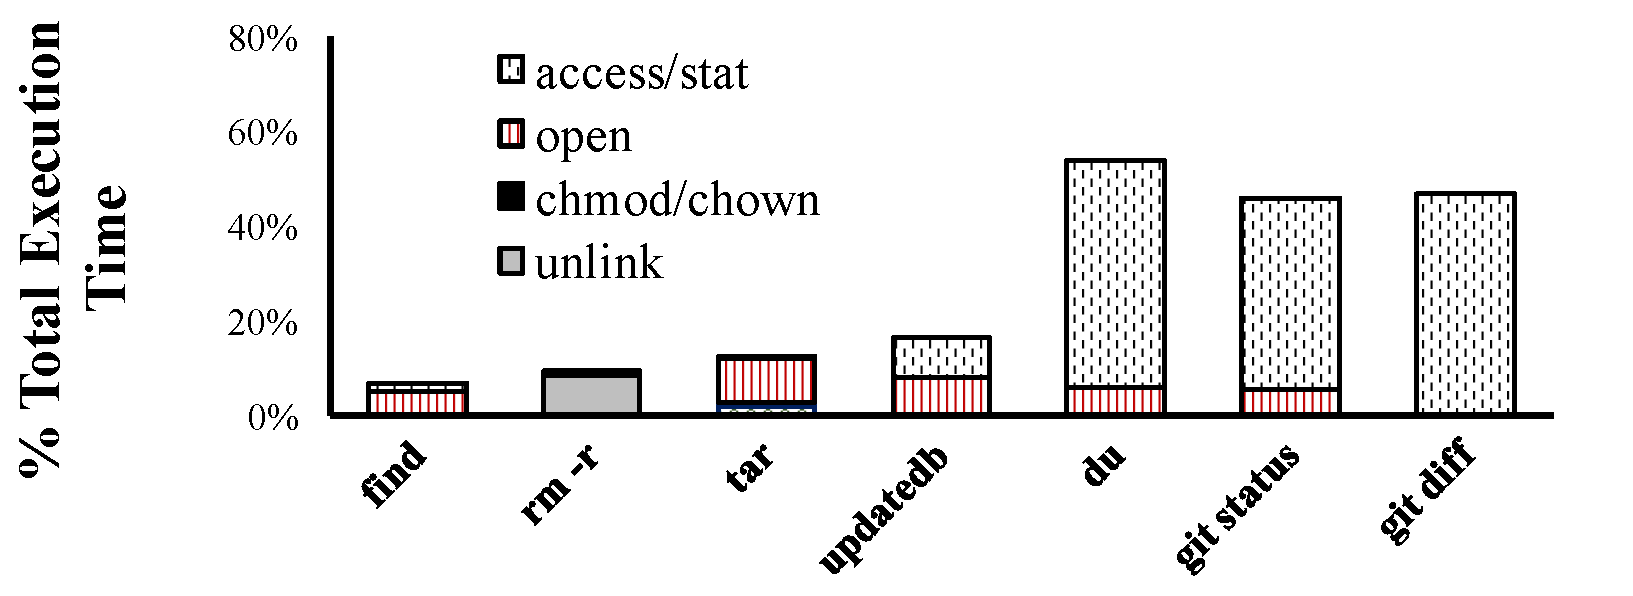
\includegraphics[width=5in]{dcache/plots/syscall-percentage.pdf} \\
\caption[Fraction of execution time on path-based system calls.]
{Fraction of execution time in several common utilities spent
executing path-based system calls with a warm cache, as measured with ftrace.}
\label{fig:dcache:lookup-frac}
%\vspace{-10pt}
\end{figure}

%\fixmedp{Please check these \% against time.  I think git diff is too high.  git status seems ok.}

Directory caches are essential for good application performance.
%Unix was designed such that ``(almost) everything is a file'',
%thus even accesses to in-memory file systems, device files, FIFOs and domain sockets
%first pass through the directory cache.
%In other words, 
Many common system calls must operate on file paths,
which require a directory cache lookup.
For instance, between 10--20\% of all system calls in the iBench system call traces do a path lookup~\citep{filenotafile}. 
Figure~\ref{fig:dcache:lookup-frac} lists the fraction of total execution time
%, as well as system time, 
several common command-line applications spend executing path-based system calls
(more details on these applications and the test machine in \S\ref{sec:dcache:eval}).
We note that these system calls include work other than path lookup,
and that these numbers include some instrumentation overhead;
% are coarse measurements that include  and work than path lookup;
%, and includes some time 
%for synchronous I/O (e.g., during {\tt rename}) as well as non-path tasks (e.g., creating 
%a file handle as part of {\tt open});
nonetheless, in all cases except {\tt rm},
the system call times and counts are dominated by
{\tt stat} and {\tt open}, for which 
%can be serviced from cache and for which 
path lookup is a significant component of execution time.
For these applications, path-based system calls account for 6--54\% of total execution time.
%and 25--77\% of system time.  
This implies that
lowering path lookup latency is
 one of the  biggest 
opportunities for a kernel to improve these applications' execution time.




\begin{figure}[t!]
\centering
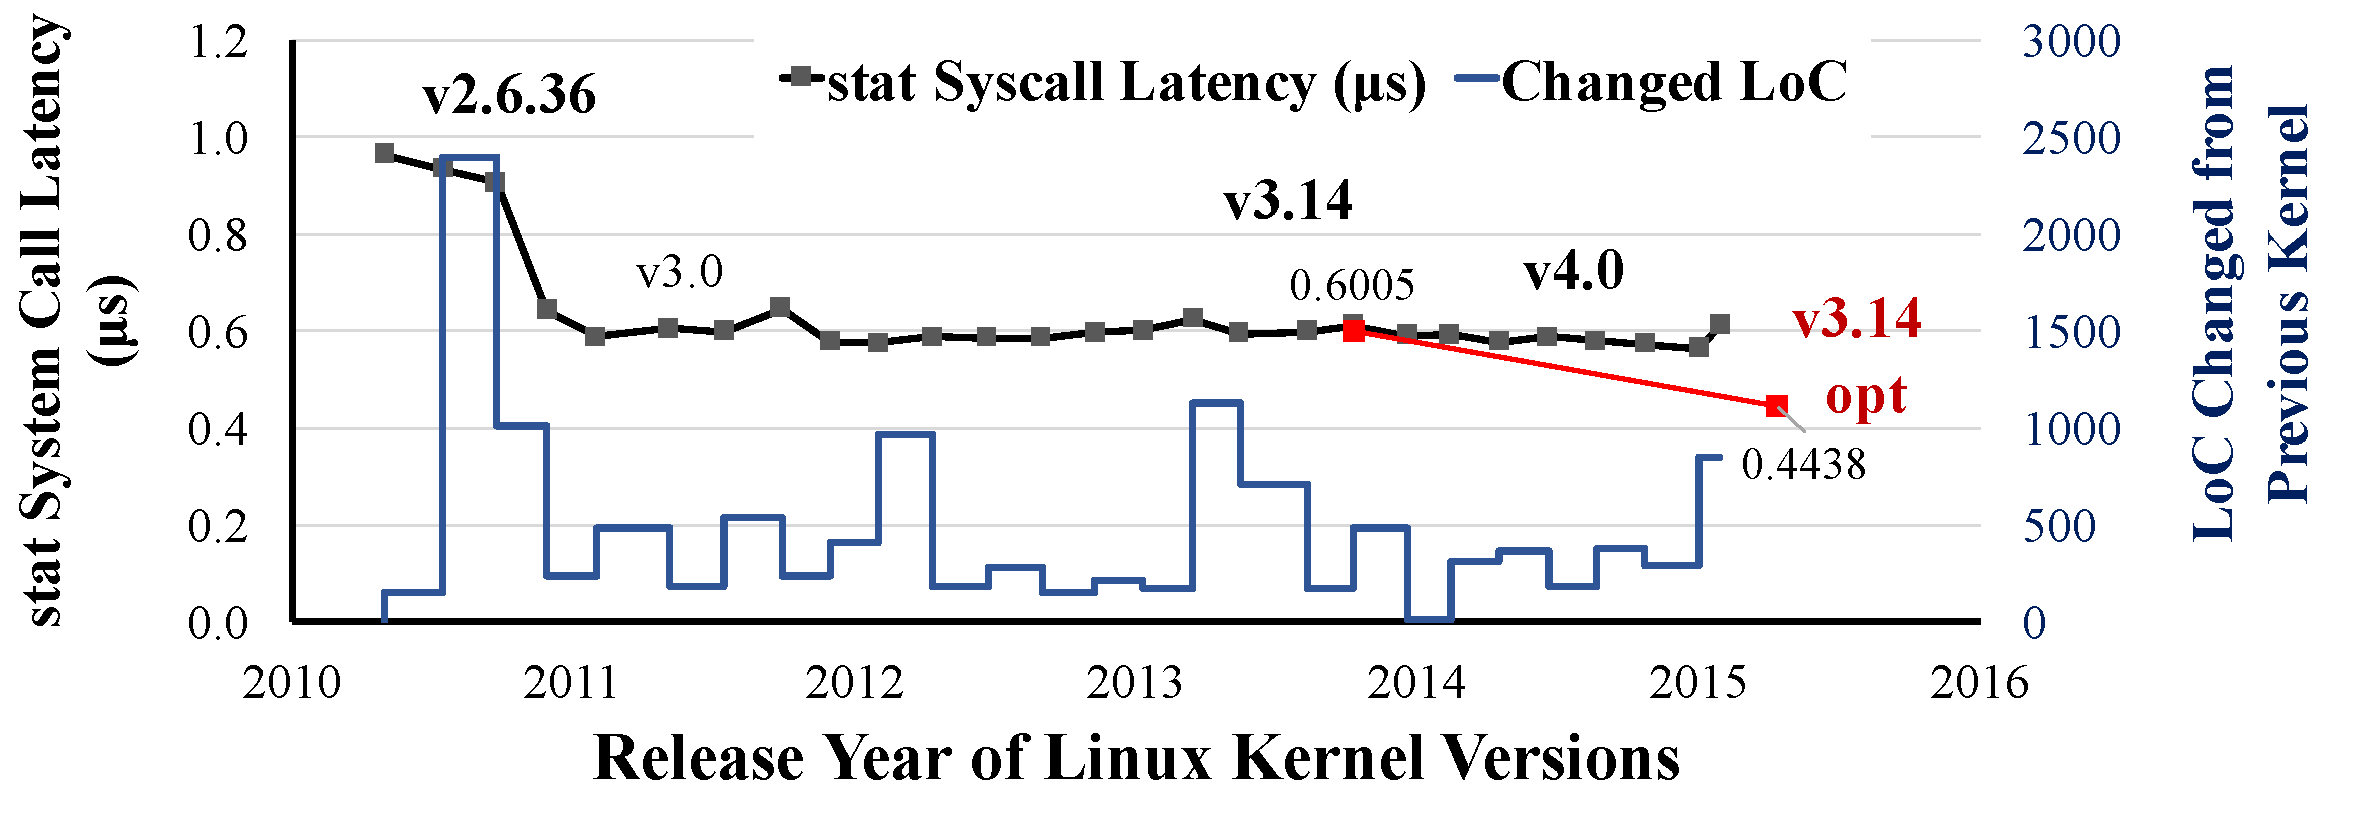
\includegraphics[width=6in]{dcache/plots/latency-by-version.pdf}
\footnotesize
\caption[Lantecy of {\tt stat} system call over years.]
{Latency of {\tt stat} system call with a long path {\tt XXX/YYY/ZZZ/AAA/BBB/CCC/DDD/FFF} on Linux over four years (lower is better), as well as the churn within the directory cache code (all insertions in {\tt dcache.c}, {\tt dcache.h}, {\tt namei.c}, {\tt namei.h} and {\tt namespace.c}). 
%Our optimizations significantly improve performance that has otherwise plateaued, despite significant ongoing developer effort.  
Our optimized \linuxver{} kernel 
further reduces {\tt stat} system call latency by \statspeedup{}\%.}
%\vspace{-15pt}
\label{fig:dcache:by-version}
\end{figure}


%\fixmedp{Add more evidence of lookup importance here: For instance, fraction of lookup time in file-related syscalls, or total lookup time in applications bound on file lookup latency.  }
Unfortunately, even directory cache hits are costly---0.3--1.1 \us{} for a {\tt stat} on our test Linux system, compared to only .04 $\mu$s for a {\tt getppid} and 0.3 \us{} for a 4 KB {\tt pread}. 
%\fixmetsai{Don, check this, I think read will be a better example, getppid is too trivial.}
This issue is taken particularly seriously in the Linux kernel community, which has 
made substantial revisions and increasingly elaborate optimizations to reduce the hit cost
of its directory cache, such as removing locks from the read path or replacing lock ordering with deadlock avoidance in a retry loop~\citep{corbet09jls,dcache-rcu}.
Figure~\ref{fig:dcache:by-version} plots directory cache hit latency against  lines of directory cache code changed 
over several versions of Linux, using a path-to-inode lookup \microbench{} on the test system described
in \S~\ref{sec:dcache:eval}.
These efforts have improved hit latency by 47\% from 2011 to 2013, but have plateaued
for the last three years.
%\fixmedp{if time, filter irrelevant changes from code deltas}
%at the cost of substantial developer effort.
%This latency appears to have plateaued 

The root of the problem is that the POSIX path permission semantics
seemingly require work that is linear in the number of path components,
and severely limit the kernel developer's implementation options.
%The root of this problem is that current directory cache
%designs reflect a straightforward implementation of the POSIX specification,
%which would seemingly require work that is linear in the number of path components.
For instance, in order to open file {\tt /\fnone{}/\fntwo{}/\fnthree{}} 
%for reading, 
one must have search permission
to parent directories {\tt /}, {\tt /\fnone{}}, and {\tt /\fnone{}/\fntwo{}},
as well as permission to access file {\tt \fnthree{}}.
The Linux implementation %of this specification is straightforward, 
simply walks the directory
tree top-down to check permissions.  
Unfortunately, when the critical path is dominated by 
walking a pointer-based data structure, 
including memory barriers on some architectures for multi-core consistency, 
modern CPUs end up stalling on hard-to-prefetch loads.
Moreover, because so many Linux features are built around this behavior, such as Linux Security Modules (LSMs)~\citep{wright+lsm},
namespaces, and mount aliases, it is not clear that any data-structural enhancements
are possible without breaking backward-compatibility with other Linux kernel features.
A priori, it is not obvious that a faster lookup algorithm, such as a single hash table lookup, 
can meet these API specifications and kernel-internal requirements; to our knowledge,
no one has tried previously.

%This paper proposes a decomposition of the directory cache, which allows
%most lookup operations to execute with a single hash table lookup (\S\ref{sec:dcache:dcache}),
%as well as optimizations to reduce the miss rate based on information that is {\em already in the cache}, but not used effectively (\S\ref{sec:dcache:readdir}).
%Our design maintains compatibility (\S\ref{sec:dcache:generalize}) through 
%several essential insights, including 
%how to separate the indexing of paths from checking parent permissions,
%and how to effectively and safely memoize the results of access control checks.


%% This paper proposes several new ways to organize a directory cache, which can yield 
%% substantial performance improvements over the current state of the art.
%% %This paper demonstrates that, despite this developer effort, there is still a substantial 
%% %missed opportunity hiding behind historical, intuitive, but not fundamental design choices.
%% Most of the Linux directory cache design reflects a straightforward implementation of the POSIX 
%% specification. %, with a division of labor that is suitable for mainstream file systems.

%This paper presents an alternative directory cache organization, which 
%improves performance by separating logical tasks, such as separating path indexing from permission checking; yet the design is sufficient to retain compatibility with POSIX.
%In the case of path lookup, 
%this paper demonstrates how 
%a per-component tree walk can be replaced with a single hash table lookup (\S\ref{sec:dcache:dcache}).
% without violating POSIX compliance.

%Our optimizations improve the performance of frequent lookup operations, but 
%introduce several costs, described in \S\ref{sec:dcache:dcache} and measured in \S\ref{sec:dcache:eval},
%which  we believe are acceptable and a net improvement for applications.
%First, these optimizations slow down infrequent modifications to the directory hierarchy, such as {\tt rename}, {\tt chmod},
% and {\tt chown} of a directory. 
%However, these slower operations
%account for less than .01\% of the system calls in the iBench traces~\citep{filenotafile}.
%Second,  the memory overheads of the dcache are increased.
%%(45\% per \dentry{}, as well as some  in our prototype).
%%(\fixmedp{XX MB} in our tests).  
%Third, lookup has a 
%probability of error from signature collisions that can be adjusted to be negligible
%%($2^{-141}$ in our configuration), 
%and within acceptable thresholds widely used by data deduplication systems~\citep{Debnath:2010:CSU:1855840.1855856, Srinivasan:2012:ILI:2208461.2208485, Quinlan:2002:VNA:645371.651321, Zhu:2008:ADB:1364813.1364831}.
%%, as well as how to remove
%%all memory barriers from the lookup path (\S\ref{sec:dcache:update}).
%In the micro-benchmark of Figure~\ref{fig:dcache:by-version}, our directory cache 
%optimizations improve lookup latency by 
%%revisions improve latency of accessing a long path
%%by 
%\statspeedup{}\% over unmodified Linux.
%%Our design addresses other missed
%%opportunities, such as identifying new opportunities to reduce the miss rate
%%through caching directory completeness.
%%\fixmedp{Do we want to highlight LoC?  3K is more than anything in the graph} \fixmetsai{Probably just mention in the evaluation. It's a metric that we should provide, but it's not awfully interesting.}
%%The total lines of code changed are fewer than 3,000 out of \fixmedp{XX}.
%%\fixmedp{Can we get 
%%, yet changes fewer than 3,000 lines of code.

%% SOSP cut - kind of long-winded
\begin{comment}
This paper rethinks current Linux directory cache design choices in light of the following goals:
\begin{compactitem}
\item {\bf Minimize the cost of a cache hit.} (\S\ref{sec:dcache:dcache}).
This means maximizing the benefit of temporal locality for frequent operations,
while pushing extra work of consistency maintenance onto less frequent, already-expensive operations.
%such as handling cache miss or updating massive metadata,
%in order to improve very frequent operations.
\item {\bf Maintain legacy compatibility.} (\S\ref{sec:dcache:generalize}).  Unix path semantics are complex, required by applications, file systems, and security modules, frustrating otherwise straightforward optimizations.  However tempting it may be to redesign path behavior to facilitate caching, path operations must exhibit the same behavior, with lower latency.
\item {\bf Never miss the same request twice in quick succession.} (\S\ref{sec:dcache:readdir}).  A number of less-frequent operations, such as reading a directory or secure temporary file creation, always miss in the cache {\em even if enough information is in cache to satisfy the operation.}  
%Of course, infrequent accesses should still be subject to a cache replacement policy, such as LRU.
\end{compactitem}
%Although directory caches must implement more complex semantics than a hardware memory cache,
%these principles should seem familiar to the reader with a basic architecture background.
%sadly, the Linux directory cache design violates all three.
\end{comment}

%This paper introduces several techniques to improve the performance of a directory cache,
%This paper explains several practical directory cache optimizations,
This paper demonstrates that these techniques improve performance for applications that use the directory cache heavily,
and the harm is minimal to applications that do not benefit.
%and that the worst case \microbench{} is only 12\% slower within \fixmedp{XX}\% of unmodified Linux.
%Each optimization we describe improves performance in isolation, and all can be combined.
%These optimizations change very few lines of code, and are backward-compatible with 
%legacy applications.  
%These changes are encapsulated in the VFS---individual file systems do not have to change their code.
%This paper describes a  prototype of these improvements implemented in Linux \linuxver{}.
%\S~\ref{sec:dcache:background} explains that the directory cache structure of Mac OS X, FreeBSD, and Solaris 
%are sufficiently similar that these principles should generalize.
%we compare and contrast Linux's directory cache
%with Mac OS X, FreeBSD, and Solaris in \S\ref{sec:dcache:background}, and explain inline how each
%optimization could be generalized to these other OS kernels.





%% \item {\bf Modularization and stackability}:
%% Any changes or optimizations must be implemented as modules inside Linux's VFS,
%% and can be stacked on top of the original design or any future optimizations. 
%% \item {\bf Backward compatibility}:
%% Any changes or optimizations must maintain least requirement of modifying any
%% file systems.
%% \item {\bf Generalization to other OSes}: Any changes or optimizations must be portable to other OSes with reasonable effort and change of design.




%% \dcache{} is proven to be effective on improving storage performance.
%% Experiments shows that,
%% in a Linux 3.x kernel, a \dcache{} with a xxx\% hit rate can speed up
%% metadata lookup and fetching time by xxx times.
%% \fixmetsai{experiment result, Linux version, and fs specs here}
%% However, we observed that Linux maintainers have made
%% constant and non-trivial efforts to improve \dcache{} in the Linux kernel.
%% We studied all \dcache{}-related source files in the Linux kernel Git repository,
%% and discovered that maintainers have committed
%% on average xxx revisions per source files.

%% We tested metadata lookup time on primary \dcache{}-related revisions.
%% Most changes on \dcache{} system only create xxx\%-xxx\% speed-up
%% than their predecessor.
%% \fixmetsai{result and graph here}.
%% Moreover, improvement to \dcache{} is still work-in-progress
%% for Linux maintainers.
%% \fixmetsai{reference to threads for latest dcache discussions}. 
%% All the evidences show that,
%% despite of significant reduction of storage operations,
%% efficiency of \dcache{} system internally still remains as a concern.

%% We argue that the design of \dcache{} needs to be carefully re-examined,
%% to fundamentally identify any missed opportunities that
%% improve value of \dcache{}.
%% At a high level, most optimization works for \dcache{} are focused on
%% improving ``how to cache'',
%% but we want to also lay eyes on ``what to cache'',
%% to ensure any valuable information returned from file systems
%% be captured by \dcache{} system.

%The contributions of this paper are as follows:
%\begin{compactitem}
%\item A performance analysis of the costs of path lookup and the opportunities
%to improve cache hit latency.
%\item A directory cache design that improves path lookup latency with a combination of techniques, including:
%  \begin{compactitem}
%  \item Indexing the directory cache by full path, reducing average-case lookup from linear to constant in the number of path components.
%  \item A Prefix Check Cache (PCC) that separates permission checking from path caching.  The PCC memoizes permission checks, and is compatible with LSMs~\citep{wright+lsm}.
%  \item Reducing the cost of checking for hash bucket collisions with path signatures.
%  \end{compactitem}
%\item Identifying opportunities to leverage metadata the kernel already has to reduce miss rates, such as tracking whether a directory is completely in cache.
%\item Carefully addressing numerous, subtle edge cases that would frustrate rote application of these techniques, such as integration with symbolic links and Linux namespaces.
%\item A thorough evaluation of these optimizations.  For instance, our optimizations improve throughput
%of the Dovecot IMAP server by up to \dovecotspeedup\% and latency of 
%updatedb by up to \updatedbspeedup{}\%.
%%git version control system by up to 25\%.
%
%\end{compactitem}

\papersection{\Thehostabi{}}
\label{sec:overview:host}

\issuedone{1.1.b}{Describe \thehostabi{} specification}
The development of \graphene{} starts with defining a simple host ABI (application binary interface) called \thehostabi{},
containing only OS abstractions essential to target applications.
%and is easily ported to different platforms.
%and minimal specifications for the host OSes and hardware.
%The host ABI is a new boundary between OSes (or hypervisors) and applications.
\Thehostabi{} separates
the implementation of an existing system API (application programming interfaces), which determines the compatibility against applications,
from hardware abstraction features, such as file systems, network stacks, and device drivers. 
\graphene{} moves the system API components
to a \libos{} in the userspace and reimplements the functionality using \thehostabi{}.
To port \graphene{} to a new host OS or hardware,
OS developers only have to implement \thehostabi{} on the target host system API,
%to new host OSes and hardware,
instead of paying a tremendous cost to translate the whole system API specification. Figure~\ref{fig:overview:porting} illustrates the porting process of \graphene{}.



%The host ABI separates the low-level, hardware management features, from the idiosyncrasy of system interface. 
%\graphene{} moves the upper layer of OS components,
%including the system calls and namespaces, into an library OS,
%leaving \thehostabi{} 
%as a narrowed interface to the host OSes and hardware.
%The host ABI intends to minimize the development effort on each host OS or hardware
%to mitigate the interface distinctions,
%to simply porting the OS abstractions defined in \thehostabi{}.


\begin{figure}[t!]
\centering
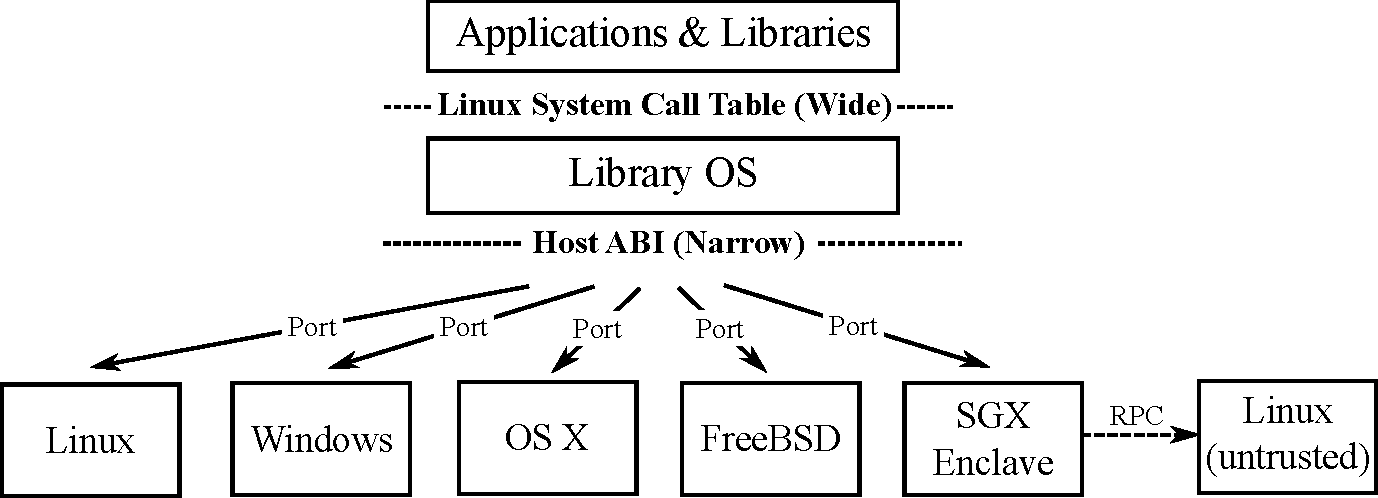
\includegraphics[width=30em]{porting.pdf}
\caption{Porting model of \graphene{}.}
%\vspace{-.1in}
\label{fig:overview:porting}
\end{figure}



\papersubsection{Platform Adaption Layers (PALs)}
\label{sec:overview:host:pal}


For each host OS or hardware, \graphene{} uses
a thin library called a {\bf platform translation layer (PAL)}
to translate among host interfaces.
%is loaded below the library OS, to translate each functions in \thehostabi{} to native system interfaces.
The main purpose of a PAL is to mitigate the semantic gap
between \thehostabi{} and
native host system APIs.
%The effort of PAL development is per host OS, whereas the library OS implementation is reusable on every hosts. %The simplicity of \thehostabi{} can be also estimated by the effort of implementing a PAL for each host.
By implementing a PAL on a new host OS or hardware,
users can reuse
the same \libos{} to run the same collection of unmodified Linux applications.
%To keep the porting effort low,
%the development of a PAL must be straightforward
%for average OS developers.
%to achieve with limited efforts.
%Based on the principle of porting simplicity, PAL development must be straightforward
%for average developers.







%The host ABI is defined for the simplicity of porting, as well as the sufficiency for implementing a library OS compatible to Linux.
%First of all, the number of host functions included in \thehostabi{}
%is much smaller than the number of system calls in a commodity OS such as Linux. 
\graphene{} currently contains PAL implementations for several popular OSes,
including Linux, \win{}, \osx{}, and FreeBSD.
%and \sgx{} with an untrusted Linux kernel.
Most of these OSes provide a POSIX-like system API similar to \thehostabi{}.
Due to the similarity, translating most of \thehostabi{} to one of the system APIs
are straightforward for average OS developers.
\Thehostabi{} is also much smaller than the actual POSIX API, making it extremely portable.



A part of \thehostabi{} may be challenging to port
on an OS,
due to unexpected system assumptions made by the OS.
For instance, \win{} does not support
fine-grained memory deallocation for de-privileged applications.
To implement system calls like \syscall{munmap} and \syscall{mprotect},
\graphene{} needs host ABIs to
deallocate or protect virtual memory pages at page granularity.
%A workaround is to change memory mappings at the physical page level,
%but will require running the \win{} PAL with root permissions.
%This type of porting challenges
%tends to be results of design decisions or assumptions made by OS developers.
%A \libos{} can potentially design
%different emulation strategies
%to compensate missing host abstractions.
A few host abstractions such as a bulk IPC feature are
optional to the host ABI;
if a host OS does not support these abstractions,
the \libos{} must fall back to alternatives. 

%In our experience, the development of a PAL is around ten thousand lines of code.

%For each port, the amount of code written for implementing \thehostabi{} is at the order of magnitude of thousands of lines of code, which is much more manageable than implementing a flat translation layer for system interfaces.


\begin{comment}
Based on the experience in \graphene{},
it is hard to ensure the portability of \thehostabi{} on every potential hosts.
%even a host ABI specialized for simplicity cannot guarantee to be portable on every hosts.
A host may simply lacks the functionality
for implementing a \hostapi{}.
The assumption is, maintaining the compatibility of \thehostabi{} poses a much less challenge than maintaining the whole system API.
Besides, the library OS may flexibly switch among emulation strategies
to compensate the absence of certain host abstraction.
As an example,
bulk IPC is optional in \thehostabi{} since its first definition,
due to the expectation
that implementing the feature may not be feasible on some hosts.
If bulk IPC is not available,
the library OS can fall back to RPC-based IPC, with a reasonable amount of performance penalty.
In the worst case, if there is no emulation strategies
to compensate for the absence of a \hostapi{},
user can predict the affected applications and avoid running these applications
on specific hosts. 
%at least users can predict whether an application will be affected and thus cannot run on certain hosts.
\end{comment}


%For a host OS that does not support ELF binaries, the PAL must follow the binary format which the host OS accepts, such as the Portable Executable (PE) format on \win{}.
%The PAL is the only layer in the user space which cannot be reused
%across different hosts. Besides the PAL, all of the other binaries in the user space are fully reusable, including the library OS, the supporting libraries, and the application executable.



%The host abstractions map to several common system calls in a commodity OS.
%For example, \funcname{StreamRead} and \funcname{StreamWrite} can directly map to the POSIX functions \funcname{pread} and \funcname{pwrite}, which are available in most OSes including Linux, BSD, \osx{}, and \win{}.
%More than half of the functions in \thehostabi{} can be counted toward this category.
%The rest of the host abstractions are either specific to Linux
%(e.g., TLS support),
%or belong to the POSIX functions that are not shared with commodity OSes
%(e.g., \funcname{mmap} on \win{}).
%The PAL emulates these host abstractions, using existing system interfaces available on the host OS, unless the software emulation is fundamentally impossible (e.g., restricted by the system interfaces), or too expensive (e.g., high overhead from copying data).



\papersubsection{Definitions and design principles}
 

\graphene{} defines \palcallnum{} calls in \thehostabi{} (also called \hostapis{}),
with a set of host abstractions
sufficient for \libos{} development.
%The host ABI defines the interaction between the library OS and a specific host.
%The \graphene{} library OS can be deployed on any ``host'' where \thehostabi{} has been ported.
This thesis defines
a {\bf host} of \thehostabi{}
to be an OS or hypervisor
which contains enough OS functionality for running a standalone application or virtual machine.
Most of the host targets in \graphene{}
are monolithic OSes,
including Linux, \win{}, \osx{}, and FreeBSD.
%which has defined a massive system API for programmability.
A monolithic OS 
usually contains a massive amount of system APIs,
which is sufficient for
implementing \thehostabi{}.


A special example of a host
is an \sgx{} (Software Guard Extensions) enclaves~\cite{intelsgx},
which
restricts OS functionality for security reasons.
The restrictions on \sgx{}
are results of a strong threat model
which distrusts any OS features except ones that are virtualized by the CPUs or migrated into enclaves.
The only way to obtain any missing OS features such as storage or networking
is to request through RPC (remote procedure call).
Requesting untrusted OS services through RPC also introduces new security threats that application developers tend not to anticipate~\cite{checkoway13iago,osdi16scone}.
Due to all the compatibility and security challenges discussed above,
this thesis uses \sgx{} as a representative example of a host
with unusual assumptions (e.g., threat models) and restrictions
compared to a monolithic OS.

%An innovative hardware abstraction like \sgx{} (software guard extensions)
%imposes unique assumptions and restrictions
%on a commodity OS,
%%creates a special host on top of Linux or \win{},
%%with unique interfaces and specifications regarding the host OSes.
%and thus creates a special host above the OS.

%If an OS has mutated or tweaked the interface for a hardware platform,
%such as an \sgx{} enclave 
%running on an untrusted Linux kernel,
%the combination of the OS (Linux) and the hardware platform (\sgx{}) is considered a specialized host.
%Especially, the \sgx{} port of \thehostabi{} faces several unique challenges,
%which will be discussed in Chapter~\ref{chap:sgx}.


\begin{comment}
%\fixme{each sentense should be a paragraph; starting the 2nd sentence}
\fixmedp{start with a strong opening stating the rationale}
The host ABI of \graphene{}
define functions needed from a host, in order to implement the library OS for reusing applications.
%to reuse an application and all its supporting libraries, including the \graphene{} library OS.
Each host of \graphene{} contains an OS and a hardware platform, either of which causes compatibility issues for running unmodified applications.
OS developers can port the library OS to a new host,
by simply reimplementing the narrowed host ABIs using abstractions available on the host.
%a new host platform.
%For each host which requires the compatibility for unmodified Linux applications, one only has to implement the narrowed host ABIs,
%instead of reimplementing the bloated, ``legacy'' system interfaces
%needed by the applications.
By implementing \thehostabi{}, OS developers skip the painful process of rebuilding the whole system interfaces of a commercial OS such as Linux.
The host ABIs strictly decouples the porting effort on the hosts from the compatibility feature for applications.
%The host ABIs decouple the OS development in the host and the implementation of compatibility for the existing Linux application.
What \thehostabi{} exposes is a simplified extended machine,
similar to a para-virtualization interface, capable of running the library OS as a lightweight virtual machine. % with compatibility against Linux applications.
%on which another layer of virtualization (i.e., the library OS) can be built to reproduce the compatibility for Linux.
\end{comment}


\begin{comment}
Two design principles drive the definition of \thehostabi{}s:
{\em simplicity} (i.e., easy to port on any hosts)
and {\em sufficiency} (i.e., containing enough OS functions for implementing a library OS).
The process of deciding \thehostabi{}s is comparable to
finding a ``pinch point'' within a OS implementation,
which can conveniently mediate a significant portion of OS execution paths for managing hardware abstractions.
%The two principles drive the development of \thehostabi{}s,
%The whole development of the \graphene{} library
%must be disciplined
%on extending \thehostabi{}s only when it is strongly required.
%of restraining extensions to \thehostabi{}s unless absolutely necessary.
The two principles
determine the soundness of the \graphene{} approach to improving compatibility
for any hosts.
\end{comment}


%%The host ABI is defined with partitioning in mind.
%\Thehostabi{} 
%determines a boundary which partitions several upper-level OS components, %, such as system calls and namespaces,
%into a library OS,
%%, as a dynamically-linked library which can be deployed
%%to various hosts.
%%The rationale behind the partitioning is based on the fact that not every OS component is equally important to compatibility, for applications which need to be ported across hosts.
%%When an OS is extended for a new hardware,
%%these OS components usually remain unchanged, or are predominantly reused.
%%Partitioning
%%into a library OS further guards these 
%in order to isolate the host idiosyncrasy. % on specific hardware. %any potential changes for adopting new hardware.
%%Similar isolation
%%exists in traditional OSes, but without partitioning:
%The strategy
%is also used in OSes:
%An example is the Linux virtual file system (VFS), an internal interface
%which encapsulates operations of file system drivers.
%%On the other hand,
%%drivers (e.g., drivers for file systems, block devices, or network cards)
%%and architecture-specific instructions
%%stay encapsulated in the host OS.
%%in the Linux kernels are usually encapsulated under a virtualized, in-kernel interface (e.g., the Linux virtual file system),
%%to simplify the development of the rest of the kernel.
%Similar to VFS,
%\thehostabi{} is intended
%to be a more ubiquitous interface,
%which encapsulates
%any host-specific behavior and semantic
%inside the host OS.
%%for encapsulating both OS and hardware idiosyncrasy on a wide range on hosts.
%%declares a ubiquitous system interface, to encapsulate both OS and hardware abstractions
%%for the library OS.




\Thehostabi{} shares several characteristics with a virtual hardware interface
exported by a hypervisor.
A generic, backward-compatible
virtual hardware interface
%a set of generic, virtual hardware,
%which the VM can control with the same drivers.
allows an unmodified OS kernel to run inside a virtual machine as on the bare metal.
%by exporting interfaces close to commodity hardware.
%To avoid additional porting effort, the virtual hardware are close to the typical commodity hardware.
%For instance, a virtual hardware interface
%usually includes a virtual NIC (network interface controller),
%such as the virtualized E1000 interfaces
%available in VMware workstation or QEMU.
%As a result, \thehostabi{} contains the
%typical OS features and interfaces, similar to the API of early UNIX systems.
The key difference between
a virtual hardware interface
and \thehostabi{}
is that \thehostabi{} does not target reusing a whole, unmodified OS kernel as a guest.
Instead, 
\thehostabi{} contains higher-level abstractions such as files and network sockets
to ensure portability on most host OSes.
The concept
of defining \thehostabi{}
with a customized guest OS (i.e., a \libos{}) running atop \thehostabi{} is similar to para-virtualization.
%\thehostabi{} expects the \libos{}
%to be rewritten and
%customized for \thehostabi{},
%similar to a 
%para-virtualizated VM.
%Compared to an actual para-virtualized VM,
A para-virtualized VM defines hypercalls as interfaces between a guest OS and a hypervisor.
Furthermore, \thehostabi{} avoids duplication of OS components
such as scheduler, page fault handler, file systems, and network stacks
between the host and \libos{}.
%Another difference is that \thehostabi{} is called by normal function calls, whereas para-virtualization relies on hypercalls.
To compare a VM and a \libos{} on a spectrum,
a VM reuses a whole OS on a wide, backward-compatible virtual hardware interface
whereas a \libos{} implements only system API components on a simplified host ABI.

The following paragraphs discuss the key design principles of \thehostabi{},
including porting simplicity, sufficiency for \libos{} development, and ease of migration.

\paragraph{Porting simplicity.}
%To reduce porting effort
%\thehostabi{}
%must be simple to port on a host OS or hardware.
To reduce porting efforts,
\graphene{} defines \thehostabi{}
using two strategies:
first, \graphene{} significantly reduces both the size and complexity of host OS features
that OS developers have to implement.
Effectively, \graphene{} avoids duplicated OS features and handling rare corner cases
on \thehostabi{}.
%The development of \graphene{} disciplinarily avoiding adding any functions to \thehostabi{},
%unless the library OS cannot internally implement an OS feature.
Second, the definition of \thehostabi{}
imitates common system APIs in a POSIX-like monolithic OS,
to directly translate most calls to
a few similar host abstractions.
%existing system calls or system library functions
%on each host.
%include functions which can be directly mapped to OS functions exported by the host.
%%the likelihood of finding similar features on the host, to be translated to functions in \thehostabi{}.
%The assumption that such a strategy is possible
%is based on
%the observation that
%%similarity of system interfaces is common among most OSes.
%similar OS functions, especially UNIX-style APIs,
%tend to commonly exist in most OSes.
%, to reduce the learning curve for programming applications.
For instance,
the stream APIs in \thehostabi{}, such as \palcall{StreamRead} and \palcall{StreamWrite}
are similar to
system calls like \syscall{read} and \syscall{write} exist on Linux, BSD, and POSIX API,
or \syscall{ReadFile} and \syscall{WriteFile}
on \win{}.
%with similar functionality and semantics.
%and 
%looks similar to \syscall{ReadFile} in \win{}, except the data types.
%The definition of \thehostabi{}
%is based on observations of the system interfaces in some of the important hosts,
%including Linux system calls and \win{} API.
%exported by the targeted hosts,
%and defines the functions in \thehostabi{}, to be easily translated to the native system interfaces.
%The host ABI is essentially a subset of the common features from every potential hosts.
%We expect %\thehostabi{} defined with simplicity in mind
%to be straightforward to port on most hosts,
%Most functions in \thehostabi{} can be easily translated to host system interfaces
%in various styles.
As the rest of this thesis proves, porting \thehostabi{} is straightforward
on most monolithic OSes.

%For example, \thehostabi{} defines \syscall{StreamRead} and \syscall{StreamWrite} for accessing I/O streams, similar to .
%xcept some nuanced details like order of parameters.


% by including OS functions , such as \syscall{FileRead} and \syscall{FileWrite}, similar to the Linux system calls, \syscall{pread} and \syscall{pwrite}.




\begin{comment}
The simplicity of \thehostabi{}s requires retaining a minimalist design of host functions. %, based on typical OS services for managing hardware.
%\graphene{} reduces the host functions
%to the bare minimum.
The host ABIs should only contain operations that
are absolutely necessary for requesting external hardware abstractions.
%A way to simplify \thehostabi{}s is to move host functions into the library OS
%and to replace them with wrappers consisting of other host functions.
Any functions that can be partially or wholly implemented inside the library OS
should be further simplified, or even removed from \thehostabi{}s.
%---in other words, whether \thehostabi{}s can be further reduced.
Moreover, \thehostabi{}s have to be simple enough to implement on
most hosts;
%In the simplest host ABIs, none of the host functions shall be able to internally implement the behavior of another host function,
%or the definition of \thehostabi{}s is further reducible.
that is, \thehostabi{}s should contain only OS functions that are commonly offered on
most hosts.
The host ABIs are close to simplified UNIX interfaces,
such as reading or writing a file or an I/O device as a byte stream,
or creating a virtual memory mapping.
%the most common OS functions
%offered on most of the potential hosts,
For most hosts,
implementing \thehostabi{} should be as straightforward as redirecting the functions to the closest host system calls.
%such as the Linux system calls or the \win{} APIs.
For example, the functionality of \syscall{StreamRead} and \syscall{StreamWrite} in \thehostabi{}s can loosely match with
\syscall{read} and \syscall{write} in Linux,
or \syscall{ReadFile} and \syscall{WriteFile} in \win{}.
%This thesis also evaluates the simplicity of \thehostabi{}s by counting the lines of code used to implement \thehostabi{}s on each host platforms.
Since most OSes have inherited a similar design from UNIX,
it is fair to assume finding
comparable OS functions %host platforms
to \thehostabi{} would be reasonably easy.
%fair to assume that \thehostabi{}s 
\end{comment}



\paragraph{Sufficiency for \libos{} development.}
%\Thehostabi{} defines
%the host abstraction available for a \libos{} to access host hardware abstractions.
To develop a \libos{} with compatibility against a wide range of applications,
\thehostabi{}
%are demonstrated by the fact that
%the exported host functions 
contain any OS abstractions that the \libos{} cannot easily emulate.
%and a full-function library OS is implemented on top of them.
For most hosts,
the host OS abstractions
%can be categorized into five types:
include
process creation, memory management, and I/O (typically, files and network connection)~\cite{dhamdhere2007os-textbook}.
%Besides security and protection,
%the definition of \thehostabi{} is closely related with hardware management,
%and offers the most basic abstractions for each category of OS functions.
%managing specific types of hardware,
%and each contain a few basic abstractions
%which can be expanded into other system interfaces.
%For example, the basic OS functions for memory management include
%allocating (\syscall{VirtMemAlloc}),
%protecting (\syscall{VirtMemProt}),
%and deallocating (\syscall{VirtMemFree}) memory regions. % at certain granularity
%(usually in pages).
%These basic functions can be used to implement other forms of memory allocation,
%such as growing heaps with \syscall{brk}
%or allocating thread-private stacks.
%The definition of the \drawbridge{} host ABI is a hint, for creating a list of host abstractions necessary for the library OS, including streams, memory, threads, and processes. 
%If \thehostabi{}s are insufficient for implementing certain system interfaces, one may extend \thehostabi{}s with the missing functions,
%with the discipline to retain the simplicity of \thehostabi{}s.
%The extension to \thehostabi{}s must be d, to keep the extension minimal, and to avoid adding redundant functions.
%The implementation of the \graphene{} library OS demonstrates that
%\thehostabi{} is sufficient for implementing significant portion of Linux system calls.
For each type of abstractions,
a monolithic OS may define several variants of system APIs with similar functionality.
For instance, Linux provides two system calls, \syscall{mmap} and \syscall{brk}, both for memory allocation in a process.
\syscall{mmap} allocates larger memory regions with page granularity,
whereas \syscall{brk} simply grows a single, continuous heap space for more fine-grained allocation.
Many applications such as GCC~\cite{gcc}
switch among system API variants in case one of them is unavailable on certain OS distributions.
This thesis shows that,
by adopting only the semantics of one of these similar APIs or abstractions, the host OS can stay simple with
the \libos{} emulating the rest of APIs.
For instance, \thehostabi{} includes \syscall{VirtMemAlloc}
as a similar feature as \syscall{mmap},
which is sufficient to emulating both \syscall{mmap} and \syscall{brk}.



\graphene{} defines \thehostabi{} partially based on
\drawbridge{},
a library OS for single-process \win{} applications.
The host ABI of \drawbridge{} 
contains 36 functions,
%demonstrates that its host ABI is sufficient
%for running a library OS in which 99.7\% of code comes from the \win{} 7 source.
%The host ABIs of \drawbridge{} are later extended
%for running a Linux-based library OS called Bascule~\cite{baumann13bascule}.
and several works have ported the host ABI to different hosts,
including \win{}, Linux, Barrelfish, and \sgx{}~\cite{porter11drawbridge,baumann14haven,mssql-on-linux,baumann13bascule}.
%and is capable of running a library OS for single-process, Linux applications, with a few host ABI changes~\cite{baumann13bascule}.
%ill loads and links the rest of application binaries, just like the native Linux loader (i.e., \code{ld.so}).
%\graphene{} takes the high-level definitions of the \drawbridge{} and Bascule host ABIs, and customizes for general-purpose Linux applications and a wider range of hosts. 
Although running \win{} and Linux applications may face
a different set of challenges,
the nature of their APIs is mostly similar, with a few exceptions.
During the development of \graphene{}, developers found the occasions in which
the host ABI of \drawbridge{}
is not sufficient to address Linux-specific challenges
and decide to extend \thehostabi{}.
Section~\ref{sec:overview:host:abi} and Chapter~\ref{chap:abi}
will further discuss the Linux-specific extensions of \thehostabi{}.


\paragraph{Migration.}
The \graphene{} library OS shares several features of VMs, including checkpointing and migrating a running application.
Migrating a process is also the key to emulating copy-on-write forking,
on a host without physical memory sharing (e.g., \sgx{}).
A hypervisor checkpoints and migrates a VM by snapshotting the VM states above a stateless virtual hardware interface. % as a clean boundary for snapshotting the application and OS state.
\Thehostabi{} is also defined to be statelessness,
by ensuring any states in the hosts to be temporary and reproducible to the applications and \libos{}.





\papersubsection{The \hostapis{}}
\label{sec:overview:host:abi}


%\fixmedp{the beginning doesn't capture the whole paragraph.}
%The host ABI shares several common abstractions with production OSes.
%The functions in \thehostabi{}
%define the basic features needed from the hosts, to run the library OS.
%The definition of the host functions
%should be unsurprising to average OS developers,
%making the implementation on a new host to be fairly straightforward.
%The host ABI reflects the common functionality of most OSes, including Linux and \win{}.
%Although the same OS abstractions may be defined
%as different idiosyncratic system interfaces on each host OSes,
%\graphene{} takes into consideration of porting the host functions to either OSes, in the most effortless way possible.





%fixmedp{give more of the background}
Table~\ref{tab:overview:abi} lists the \palcallnum{} calls defined in \thehostabi{}:
%Among these \hostapis{}, 
25 calls are inherited from the \drawbridge{} host ABI,
including functions to managing I/O (e.g., \palcall{StreamOpen}), memory allocation (e.g., \palcall{VirtMemAlloc}), scheduling (e.g., \palcall{ThreadCreate}), and several miscellaneous functions (e.g., \palcall{SystemTimeQuery}).
%Most of the host functions only affect the OS or hardware states
%related to the process itself.
%For example, \syscall{VirtMemAlloc} can only allocate memory in the calling process,
%and cannot affect other processes running in parallel.
%Only I/O streaming functions export states to the host OS, and share states with other processes or library OSes.
14 calls are added by \graphene{}, to implement Linux-specific features.
For example, unlike \win{} or \osx{}, Linux %The host ABI is also complemented with several Linux-specific abstractions, such as
delivers hardware exceptions to a process as signals.
Linux also requires 
the x86-specific segment registers (i.e., FS/GS registers)
to determine the location of thread-local storage (TLS), which can be hard-coded in application binaries by a compilation mode of GCC.
On \win{} or \osx{}, the x86-specific segment registers are mostly ignored, and even frequently reset to eliminate attack vectors.
%The host ABI contains host functions (), which can be directly called from the library OS. \graphene{} shows that \thehostabi{} is sufficient to implementing a large portion of the Linux system calls.
%These functions are not defined in \drawbridge{}, the \win{}-based library OS,
%because these abstractions do not exist in \win{}.
%The \drawbridge{} host ABI does not contain exception delivery because the feature is
%not commonly used in \win{} applications.
%Moreover, the x86 segment registers cannot be modified in \win{}
%because the OS assigns fixed values to these registers
%for the whole execution.
%Although \drawbridge{} excludes these abstractions, Bascule extends \thehostabi{} to include similar functions,
%demonstrating that the extension is indeed necessary.
\graphene{} discovers these abstractions as a necessity for implementing a rich Linux \libos{}.



\begin{table}[htp!]
\centering
\small
\begin{tabular}{|p{.15\textwidth}|p{.33\textwidth}|p{.45\textwidth}|}
\hline
{\bf Abstraction} & {\bf Function Names} & {\bf Description} \\
\hline
\raggedright
Streams & 
\raggedright
{\tt StreamOpen} \newline
{\tt StreamMap} \newline
{\tt StreamFlush} \newline
{\tt StreamSetLen} \newline
{\tt StreamRead} \newline
{\tt StreamWrite} \newline
{\tt StreamWaitforClient} \newline
{\tt StreamAttrQuery} \newline
{\tt StreamAttrQuerybyHandle} \newline
{\tt StreamAttrSetbyHandle} \newline
{\tt StreamDelete}
& 
Opening streams using URIs, with prefixes representing stream types (e.g., \code{file:},\code{tcp:},\code{pipe:}),
as well as common stream operations, including transmission of data, and query to the stream attributes.
\\
\hline
\raggedright
Memory & 
\raggedright
{\tt VirtMemAlloc} \newline
{\tt VirtMemFree} \newline
{\tt VirtMemProtect}
& 
Allocation, deallocation, and protection of a chunk of virtual memory.
\\
\hline
\raggedright
Threads \& scheduling & 
\raggedright
{\tt ThreadCreate} \newline
{\tt ThreadExit} \newline
{\tt ThreadDelayExecution} \newline
{\tt ThreadYieldExecution} \newline
{\tt SemaphoreCreate} \newline
{\tt SemaphoreRelease} \newline
{\tt EventCreate} \newline
{\tt EventSet} \newline
{\tt HandlesWaitAny}
&
Creation and termination of threads; 
Using scheduling primitives, including suspension, semaphores, events, and pollable IO events.
\\
\hline
\raggedright
Process & 
\raggedright
{\tt ProcessCreate} \newline
{\tt ProcessExit}
& 
Creating or terminate a process with a library OS instance.
\\
\hline
\raggedright
Mis\-cel\-la\-ne\-ous & 
\raggedright
{\tt SystemTimeQuery} \newline
{\tt RandomBitsRead}
& 
Querying system time, and random number generation.
\\
\hline
\raggedright
Exceptions $\dagger$ & 
\raggedright
{\tt SetExceptionHandle} \newline
{\tt ExceptionReturn}
& 
Setting an exception handler, and returning from the handler.
\\
\hline
\raggedright
TLS $\dagger$ & 
\raggedright
{\tt SetSegmentReg}
& 
Setting the \code{FS}/\code{GS} registers.
\\
\hline
\raggedright
Remote Procedure Call $\dagger$ (optional)& 
\raggedright
{\tt StreamSendHandle} \newline
{\tt StreamRecvHandle} \newline
{\tt CreateIpcChannel} \newline
{\tt PhysicalMemoryCommit} \newline
{\tt PhysicalMemoryMap}
& 
Sending opened stream handles or physical memory across processes.
\\
\hline
\end{tabular}
\caption{An overview of \thehostabi{} of \graphene{}. The ones marked with the symbol $\dagger$ are introduced in the initial publication of \graphene{}~\cite{tsai14graphene} or later extended for this thesis. The rest are inherited from \drawbridge{}~\cite{porter11drawbridge}.}
\label{tab:overview:abi}
\end{table}

%The interfaces, as part of \thehostabi{}, which access these host abstractions, are ultimately simplified to reduce the porting effort on each host.
%Unlike the system interfaces in the OS, \thehostabi{} does not prioritize backward compatibility. Therefore, \thehostabi{} includes only the minimum interfaces that the library OS needs to interact with the host. The host ABI does not have to include any of  the legacy system interfaces from a production OS, let alone preserving different flavors of system interfaces for backward compatibility.



\graphene{} introduces five calls for 
remote procedure call (RPC) between \libos{} instances
in a multi-process application.
\graphene{} simplifies porting multi-process abstractions
on each host OS
to implementing RPCs.
The basic RPC abstraction is 
a pipe-like RPC stream for message passing between processes.
To improve performance,
%RPC is critical for implementing the coordination of OS states
%across library OS instances.
%The basic form of RPC in \graphene{} is a pipe-like RPC byte stream, which a library OS can simply use to send messages.
%It is a common design choice
%to implement inter-process coordination through message-passing
%instead of shared memory, especially for hardware platforms that do not guarantee memory coherence~\cite{baumann09barrelfish}.
%A problem to the message-passing approach is the significant overheads
%on frequently exchanging distributed OS states.
\thehostabi{} defines an optional, bulk IPC abstraction
to send large chunks of virtual memory
across processes.
%The bulk IPC feature works similarly as sending the memory through RPC streams,
%but is much faster because it avoids copying memory in the host.


%for host platforms that urgently require lowering the RPC overheads.
%Another extension is for
%%\funcname{StreamSendHandle} and \funcname{StreamRecvHandle}
%delegating opened stream handles to another process, through a connecting pipe.
%The feature is similar to sending file descriptors
%through UNIX sockets in Linux, and is used to share opened network sockets with the \syscall{fork}'ed processes.
%%Another RPC abstraction is a bulk IPC channel; a process can use \funcname{PhsyicalMemoryCommit} to commit a large chunk of memory to a bulk IPC channel, which \funcname{PhsyicalMemoryMap} can map into another process, as copy-on-write. The library OS uses bulk IPC as an optimization to \syscall{fork}.
%Despite that either of the RPC primitives
%is not necessary easy to implement on every hosts, the inclusion of these host functions is completely optional, and the library OS can always fall back to the message-passing approach.



%All the host functions are designed to appear as ``stateless''
%as possible to the library OS.
%Being stateless to the library OS means that
%a host function does not preserve any permanent state of certain host abstraction.
%A stateless function can recover
%from disconnection of the library OS, and be reconnected at any timing.
%The host functions can maintain temporary bookkeeping for the convenience of porting,
%but should not assume the bookkeeping states to be permanent.
%The principle of defining all the host functions to be stateless
%is primarily for two purposes:
%{\em migration} and {\em security isolation}.
%For migration, the fact that the library OS can disconnect freely from the host functions simplifies the implementation of the migration feature.
%Migration is also an important foundation to implementing \syscall{fork}, because the cloned process need to receive a snapshot of the parent process.
%For security isolation, 
%a stateless host function is easier to check,
%because the security monitor only has to verify each instance of host function calls,
%instead of tracing multiple host functions over a longer period of time.

%the functions to access each host abstraction must appear \fixmedp{clarify `stateless'} stateless to the host, except for the handles to identify the resources. Each call to the host functions is independent. The arguments given for each call must be always be absolute values, instead of relative values.
%For example, the offset given to \funcname{StreamMap}, \funcname{StreamRead}, and \funcname{StreamWrite} (if the opened handle is a file) are offsets from the beginning of the file, and thus are irrelevant to how many bytes that are previously written or read.
%When enforcing isolation rules, the host OS can check the arguments of each calls to the host functions, independently and atomically.


%A host ABI (application binary interface) has to define the convention of application binaries, including the binary format and the linking procedure, as well as a set of  system interfaces.
%The host ABIs contain a minimal loader which recognizes a basic version of the ELF (Executable and Linkable Format), just enough to compose a binary of the library OS.
%The very initial loading procedure as part of \thehostabi{}s only loads a clean library OS instance.
%Each host of \graphene{} is supposed implement a minimal dynamic loader,
%which can load the \graphene{} library OS binary in ELF.
%The library OS then completes the dynamic loading procedure,
%by directly loading the Linux native dynamic loader (i.e., \code{ld.so}), and indirectly loading the rest of the application binaries.







\papersubsection{Host-enforced security isolation}
\label{sec:overview:host:security}


To target multi-tenant environments, 
\graphene{} enforces strong security isolation between mutually-untrusting applications running on the same host.
The security isolation of \graphene{} is comparable to running each application
in a VM or a container.
Just as a virtual hardware interface isolating each VM,
\thehostabi{} also enforces security isolation between library OS instances.
%according to the trust model of the applications.


On a trusted host OS,
\graphene{} delegates security isolation as a host-level feature.
The library OS and the application must mutually trust each other, due to lack of internal privilege separation in a process.
%The host ABI also separates API implementation
%from security isolation.
%To ensure isolation, each host must restrict access from the applications or the library OS, to any unauthorized host abstractions.
On each host, a reference monitor enforces security isolation policies, by access control on OS abstractions sharable among processes, including files, network sockets, and RPC streams.
%The host-level security isolation is orthogonal to API complexity.
Separating security isolation from API implementation simplifies security checks
for applications that only require
complete protection from other tenants.
%based on monitoring the references to host resources and rejecting authorized resource access.
%to the host abstractions.





%\graphene{} reduces the attack surface exposed to applications
%by restricting access to the host kernel ABI 
%and prevents access to unauthorized system calls, files, byte streams,
%and network addresses with a \emph{reference monitor}.
%The host kernel ABI exported by the \pal{} heavily 
%limits the ability of a \graphene{} application to interact with the rest of the system;
%any external interactions are further mediated by a reference monitor.
%Unlike a typical Linux system, \graphene{} applications cannot interact with shared 
%system daemons or other shared system resources.
%As a result, \graphene{} enforces security isolation similar to running applications in separate VMs---even
%applications that span multiple processes.


In \graphene{},
one or multiple processes of the same application run in a {\bf sandbox}.
Multiple library OS instances coordinate
in a sandbox
to present a unified OS view
to the application.
%As the library OS instances can coordinate shared OS states using simple RPC streams,
The design simplifies the enforcement of security isolation for multi-process abstractions.
\graphene{}
uses the reference monitor to block RPC streams across the sandbox boundary,
stopping applications in different sandboxes from accessing multi-process OS states.
%\graphene{} contributes a multi-process security model 
%based on the abstraction of a \emph{sandbox},
%or a set of mutually trusting processes.
%If a reference monitor exists, the reference monitor permits the processes within the same sandbox to communicate and exchange RPC messages, but disallows cross-sandbox communication.
The current design focuses on security isolation, although we do expect to extend the design for more sophisticated policies
in the future.

\begin{comment}
The only host abstractions that are shared across processes and must be mediated by the host for isolation are files, network sockets, and RPC streams
--- all other allowed host ABI modify only local process state, such as VMAs and threads.
%Thus, the reference monitor need only mediate file access, socket and RPC stream creation.
%an unprivileged daemon
%as well as extensions to the App\-Armor LSM~\cite{apparmor},
%which checks file and socket policies in the kernel.
%, reducing context switching overhead
%and the risk of race conditions~\cite{garfinkel03traps}.
In order for the reference monitor to restrict file access, socket and RPC stream creation,
each application includes a {\em manifest file}~\cite{hunt07rethink},
which describes a {\tt chroot}-like, restricted view of the local 
file system (similar to Plan 9's unioned file system views~\cite{pike90plan9}),
%including read-only shared files,
as well as {\em iptables}-style~\cite{iptablesman} network firewall rules.
To facilitate sharing read-only libraries, a manifest may specify a file system view which combines several different sub-directories of the local file system, and can prevent writing to files or directories.


For example, the \graphene{} reference monitor on the Linux host is implemented using \syscall{ioctl} to a special device (\code{/dev/graphene})~\fixme{a prospective design}.
A process is restricted by the Linux BPF-style system call filter, or the SECCOMP filter~\cite{seccomp}, to use \syscall{open} to access any files, or to \syscall{connect} or \syscall{bind} to any sockets.
It must use the \graphene{} special device to open or create streams, so the file paths or network addresses can be checked against the sandbox rules. The kernel module as the driver of the \graphene{} special device can coexist with any Linux Security Module (LSM), such as AppArmor~\cite{apparmor} or SELinux~\cite{selinux}.


When a new process is launched by the host, it begins execution in a new sandbox.  
Child processes may either inherit their parent's sandbox, or can be started in a separate sandbox---specified by a flag to the host abstractions of process creation.
A parent may specify a subset of its own file system view 
when creating a child, but may not request access to new regions of the host file system. 
%The restrictive policy enforced on the child will be written in a new manifest file generated by the parent, and the policy will be checked by the reference monitor.
The child may also issue an {\tt ioctl} call to 
dynamically detach from the parent's sandbox. The reference monitor prevents byte stream creation across sandboxes.
%among picoprocesses
%that are not in the same sandbox.
%and restricts external connections to remote URIs according to firewall rules in the manifest.
When a process detaches from a sandbox, effectively splitting the sandbox, the host must closes all RPC streams that could bridge the two sandboxes.
\end{comment}



\paragraph{Threat model.}
For most hosts, application trusts the host OSes as well a \libos{} instances in the same processes.
For multiple processes inside a sandbox,
the \liboses{} in these processes
also trust each other.
Applications or \liboses{} are not trusted by the host OSes or processes outside of the sandboxes.
Applications and \liboses{}
can become the adversary to the host OS,
by exploiting vulnerabilities on \thehostabi{}.
%the \graphene{} design reduces the attack surface between the hosts and the library OS instances, to defend against a malicious application.

%On a host with a reference monitor, the host OS and the reference monitor are both trusted, to mediate all system interfaces used to implement \thehostabi{}. The host must check all access to any abstractions with effects outside of a process's internal state, such as an opened file, or a connected network socket.
%Processes inside the same sandbox mutually trust each other. The adversary can run arbitrary code inside of one or more processes within one or more sandboxes.
%The adversary can control all code in its processes, including the library OS and the host-specific PAL.
%{\tt libLinux} and the \pal{}. 
%We also assume a trusted reference monitor process running on the host kernel that 
%launches \graphene{} applications and mediates all system calls with external effects,\fixmedp{define precisely}

%\graphene{} ensures that %The key security property the \graphene{} design upholds is that 
%the adversary cannot interfere with any victim picoprocesses
%in a separate sandbox.  
%The \graphene{} sandbox design ensures strict isolation: 
%if the only shared kernel abstractions are byte streams and files, 
%and the reference monitor ensures
%there is no writable intersection between sandboxes,
%the adversary cannot interfere with any victim picoprocess.


The threat model of \graphene{} on \sgx{}
contains the adversary from other hosts but excludes
the host OS, hypervisor, and any hardware except the CPU from its trusted computing base (TCB).
An untrusted OS or hypervisor
potentially has lots of opportunities to invade applications or VMs,
using Iago attacks~\cite{checkoway13iago}.
The challenges of porting \graphene{} to \sgx{} is not limited to resolving the compatibility issues of enclaves but also defending applications and \liboses{} against untrusted host OSes.







%%% The only processes allowed to run as standard kernel processes (non-\graphene{}) 
%%% are the reference monitor and
%%% system administration utilities that need more kernel interfaces than the \pal{} ABI provides.
%%% Ensuring that a collaborating picoprocess correctly implements
%%% some function (such as receiving a signal),
%%% as well as preventing exploitation of vulnerabilities in picoprocesses
%%% are beyond the scope of this work.

%\graphene{} reduces the system attack surface of the host, but does not change the size of its
%trusted computing base; however, reducing the effective system call table
%size of a picoprocess does facilitate adoption of a smaller host kernel,
%which we leave for future work.


\papersection{The \libos{}}
\label{sec:overview:libos}

This section gives the overview of \graphene{}, a library OS for reusing unmodified Linux applications
on \thehostabi{}.
%Existing library OSes have established reuse of single-process applications~\cite{porter11drawbridge}.
%The library OSes map a target system API, such as the Linux system calls, to abstractions in \thehostabi{}. %The reduction of host interfaces provides portability to various platforms that can translate the interfaces to host APIs or abstractions,
%and a narrower attack surface that developers can more likely reason about.
% and supporting data structures as library functions---mapping
%high-level APIs onto
%a few paravirtual interfaces to the host kernel.
%Recent library OSes improve efficiency over full guest OSes by eliminating duplicated features
%between the guest and host kernel,
%such as the CPU scheduler, or
%eliminating guest-level multiplexing code, as the library OS supports only one application;
%even compiling out unnecessary guest kernel APIs~\cite{unikernels}.
A \libos{} is comparable to a partial, guest OS running in a virtual machine.
However, compared with an actual virtual machine, the \libos{} design of \graphene{} and previous work~\cite{porter11drawbridge,unikernels} eliminates duplicated features between the guest to the host kernel, such as the CPU scheduler or file system drivers, and thus reduces the memory footprint.
%Library OSes have also been proven useful for reusing applications on new hardware platforms, such as \sgx{} enclaves~\cite{baumann14haven}.
%% dp: This sentence seems a little premature
%In recent works, library OSes provide rich OS features for isolated contexts while the host OSes are untrusted

%% Library OSes reduce the memory requirements of running a self-contained,
%% isolated application process
%% %guest \daniela{I would replaced guest by "isolated process or group of processes (a \libos{} instance)''}
%% by orders of magnitude
%% In a cloud computing environment,
%% increasing the number of applications per server has enormous
%% economic benefits.
%% Even on a desktop or portable system, \libos{}es can reduce the overheads
%% of sandboxing untrusted code and running applications
%% designed for another OS.

%Because library OSes execute within a VM \daniela{this phrase does not read good to me because (i) it might imply the picoprocesses need hypervisor support, as misunderstood by reviewer 1 and (ii) you already emphasized the drawbacks of leveraging a VM} or lightweight process ({\em picoprocess}~\cite{xax}),
%library OSes execute with

%% dp: Daniela, great suggestion!  We need to make this situation seem more
%%     like the sky will fall without our help
A principal drawback for prior library OSes is the inability to support multi-process applications. Many existing applications, such as network servers (e.g., Apache) and shell scripts (e.g., GNU makefiles), create multiple processes for performance scalability, fault isolation, and programmer convenience.
%These applications would benefit from the efficiency and security benefits
%of a library OS.
For the efficiency benefits of library OSes to be widely applicable,
especially for unmodified Unix applications,
library OSes must provide commonly-used multi-process abstractions, such as \syscall{fork}, signals, System V IPC message queues and semaphores, sharing file descriptors, and exit notification.
Without sharing memory across processes, the library OS instances must coordinate shared OS states to support multi-process abstractions.
%To support multi-process abstractions, library OSes often have to rely on sharing OS states,
%backed by the hosts' memory sharing features.
For example, \drawbridge{}~\cite{porter11drawbridge} cannot simulate process forking because copy-on-write memory sharing is not a universal OS feature.


\begin{figure}[t!]
\centering
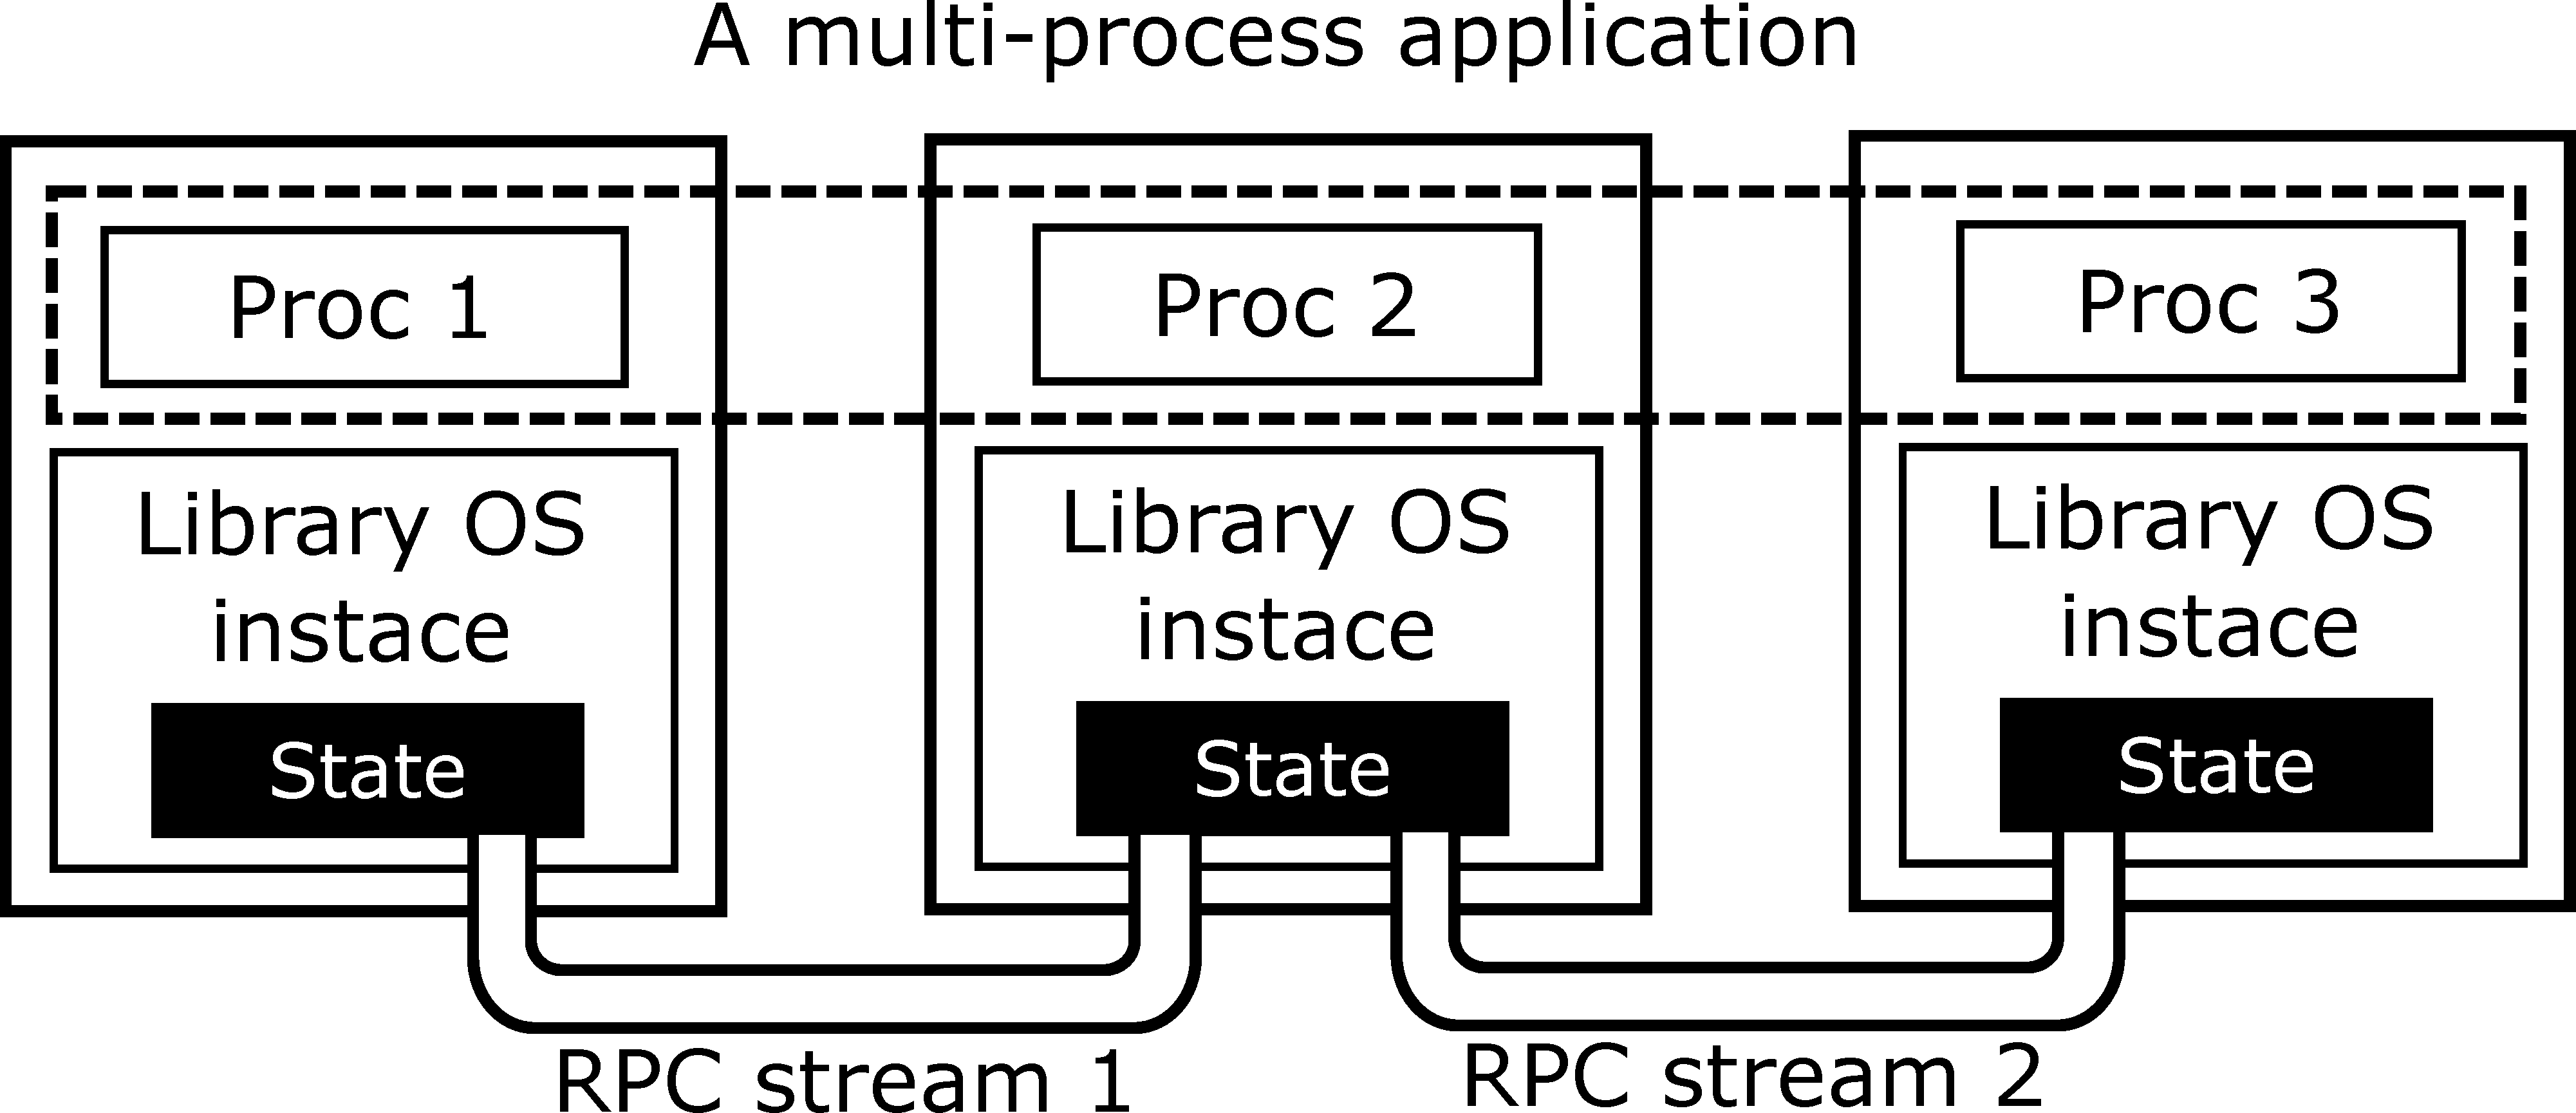
\includegraphics[width=24em]{concept.pdf}
\caption{Multi-process support model of \graphene{} \libos{}. For each process of an application, a \libos{} instance will serve system calls and keep local OS states. States of multi-process abstractions are shared by coordinating over host-provided RPC streams, creating an illusion of running in single OS for the application.}
%\vspace{-.1in}
\label{fig:graphene:concept}
\end{figure}

%{\bf \graphene{}} is a Linux-compatible library OS to run legacy, unmodified Linux applications. 
In \graphene{}, multiple library OS instances collaboratively implement
Linux abstractions, but present single, shared OS view to the application.
\graphene{} instances coordinate states
using message passing over RPC streams.
With a distributed POSIX implementation,
%placement of shared state and messaging complexity are first-order performance concerns.
%%We chose to shift implementation complexity into the library OS
%%in order to uphold simple enforcement of security isolation in the host.
%By coordinating shared states across library OS instances, 
\graphene{} can create an illusion of running in a single OS for multiple processes in an application.

%Previous library OS designs ensured security isolation of independent applications,
%comparable to a VM, by keeping a relatively narrow host ABI.
%We selected the \graphene{}
%design because it strikes a unique balance between
%and robust, flexible security enforcement.
%The \graphene{} design ensures security isolation of
%mutually distrusting, multi-process
%applications on the same host system.
%Essential to this goal is
%minimally expanding the host ABI to support multi-processing,
%as well as leveraging RPCs as a natural point to mediate inter-\picoproc{} communication.
%RPC coordination among \graphene{} instances can be dynamically disconnected, facilitating novel sandboxing
%techniques.  For instance, we develop an Apache web server extension that, upon logging in a given user,
%places the worker process's \libos{} in a sandbox with access to only that user's data.
%We expect more nuanced degrees of trust are possible in future work.

%\graphene{}'s design gives the user and system administrator a high degree of flexibility
%in isolating arbitrary groups of unmodified application processes,
%while upholding the efficiency and host compatibility benefits of recent library OSes.

%\fixmedp{After a complete draft is written, coalesce all goals and make sure they are addressed early on.  We are doing some scatter-shot motivation}


\papersubsection{\Libos{} architecture}
\label{sec:overview:libos:arch}

%Recent library OSes~\cite{porter11drawbridge,unikernels,baumann13bascule,osv}
%are designed for security and efficiency, but are limited to single-process applications.
%The security isolation of \liboses{} derives from 
%limited, explicit data sharing and 
%a narrow host interface.  
A \libos{} typically executes in either a para-virtualized VM~\cite{unikernels,osv}
% \daniela{I would have the use of a VM as a discussion topic in the end of the paper.}, 
or an OS process called a \emph{\picoproc{}}~\cite{porter11drawbridge,baumann13bascule}, with a restricted host ABI.
%The host ABI heavily restrict effects outside of the application's address space
%as a result, applications in a \picoproc{} have very little opportunity to interfere with each other,
%yielding security isolation comparable to a VM.
%The library OS deduplicates features for hardware management in both the guest and host kernels.
\graphene{} executes within a \picoproc{} (Figure~\ref{fig:overview:arch}),
which includes an unmodified application and its supporting libraries, which run alongside a library OS instance.
The \graphene{} \libos{} is implemented over \thehostabi{} designed to expose very generic abstractions that are easy to port on any host OS.
%Although the \graphene{} prototype  host kernel is Linux, 
%we adapt a host ABI from Drawbridge/Bascule,
%which has been previously implemented on \win{}, Hyper-V, and Barrelfish~\cite{porter11drawbridge,baumann13bascule,baumann09barrelfish}.
%The \graphene{} host ABI is
% summarized in Table~\ref{tab:abi} and discussed in more detail in \S\ref{sec:linux:pal}\fixmedp{if not cut...}.  
%which exposes only tens of simple host calls. \daniela{briefly define \picoproc{}: A \picoproc{} is unmodified application code running with a \libos{}.}


\begin{figure}[t]
\centering
\begin{minipage}[b]{1.25in}
\footnotesize
\raggedleft
Linux system calls \\
\graphenesyscallnum{} out of \linuxsyscallnum{}\\
\vspace{0.1in}
Host ABI \\
\palcallnum{} \hostapis{}\\
\vspace{0.2in}
\hostsyscallnum{} Linux system calls
\vspace{0.35in}
\end{minipage}
\hspace{-1.25in}
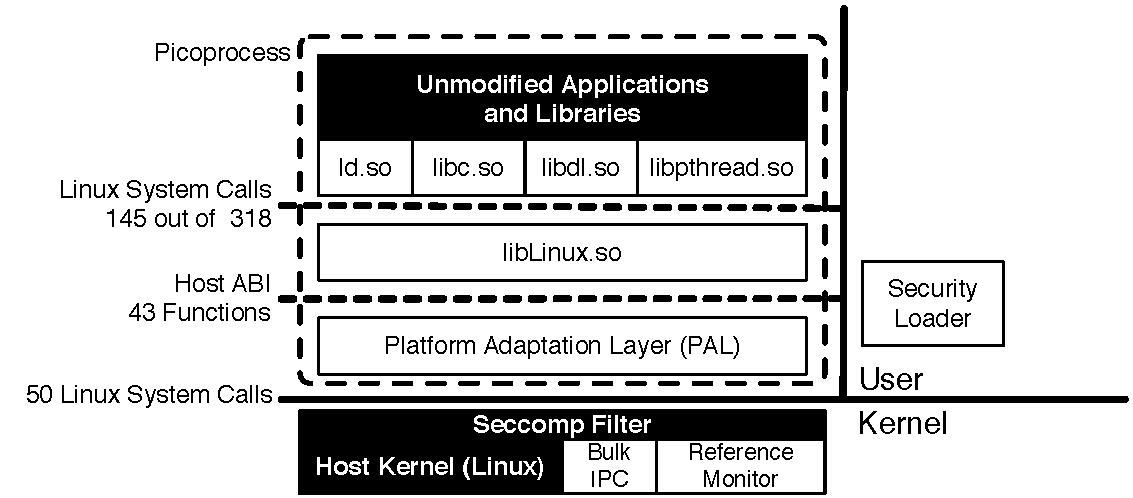
\includegraphics[width=32em]{arch.pdf}
\caption{Building blocks of \graphene{}.  Black components are unmodified.
We modify the four lowest application libraries on Linux:
{\tt ld.so} (the ELF linker and loader),
{\tt libdl.so} (the dynamic library linker),
{\tt libc.so} (standard library C),
and {\tt libpthread.so} (standard threading library), that issue Linux system calls as function calls directly to {\tt libLinux.so}.
Graphene implements the Linux system calls using a variant of the Drawbridge ABI, which is provided by the platform adaption layer (PAL).
A trusted reference monitor that ensures \libos{} isolation is implemented as a kernel module. Another small module is added for fast bulk IPC, but it is optional for hosts other than Linux.}
\label{fig:overview:arch}
\end{figure}


%\graphene{} shows the sufficiency of \thehostabi{} to support a rich Linux \libos{}.
As an example of this layering, consider the heap memory management abstraction. Linux provides applications with a data segment---a legacy abstraction dating back to original UNIX and the era of segmented memory. The primary thread's stack is at one end of the data segment, and the heap is at another.  The heap grows up (extended by \syscall{brk}) while the stack grows down until they meet in the middle.
In contrast, the host ABI provides only minimal abstractions for allocating, deallocating, and protecting regions of virtual memory.
This clean division of labor encapsulates idiosyncratic abstractions
in the library OS.


%These interfaces are host-independent \daniela{OS or kernel-independent}, as they tend to be very generic and easily
%implemented on any host OS kernel or VMM \daniela{postpone VMM for later}.

At a high level, a \libos{}
scoops the layer just below the system call table out of the OS kernel
and refactors the code as an application library.  
The driving insight is that there is a natural, functionally-narrow division point 
one layer below the system call table
in most OS kernels.
Unlike many OS interfaces, \thehostabi{} minimizes the amount of application state in the kernel, facilitating
migration. A \libos{} instance can programmatically read and modify its OS state, copy the state to another instance, and the remote instance can 
load a copy of this state into the OS---analogous to hardware registers.
A \picoproc{} may not modify another \picoprocs{}' OS states.



\papersubsection{Multi-process abstractions}
\label{sec:overview:libos:multiproc}


\issuedone{1.3.b}{An overview of multi-process support}
A key design feature of UNIX is that users compose simple utilities to create more significant applications.  Thus, it is unsurprising that many popular applications are multi-process---an essential feature missing from previous \liboses{}.
%This gap is filled by the \graphene{} \libos{}, which
%extends recent \liboses{} to support multi-process applications.
The underlying design challenge is minimally expanding a tightly-drawn isolation boundary without also exposing idiosyncratic kernel abstractions or re-duplicating mechanisms in both the host kernel and the library OS.

%requires a careful balance among the competing goals of 
%efficiency, host independence, and security isolation.
%The challenge, then, is minimal expansion of

%\vspace{5pt}
%\noindent {\bf Motivating Example.~}
For example, consider the process identifier (PID) namespace. In current, single-process library OSes, \syscall{getpid} could just return a fixed value to each application.
This single-process design is isolated, but the library OS cannot run a shell script, which requires forking and executing multiple binaries, signaling, waiting, and other PID-based abstractions.

%\paragraph{Design options.}
%Multi-process support requires extensions to the host ABI of recent, single-process library OS designs. Because multi-process abstractions, such as signals or System V IPC, tend to be idiosyncratic, an essential problem is identifying a minimal, host-independent substrate upon which  to implement OS-specific abstractions.
There are two primary design options for multi-process abstractions in \liboses{}: (1) implement processes and scheduling in 
the library OS; (2) treat each library OS instance as a process and distribute the shared POSIX implementation across a collection of library OSes.
\graphene{} follows the second option, which imposes fewer host assumptions.
%, maximize flexibility in mapping processes to physical resources, and facilitate inter-process security policy enforcement. % as enforcing security policies on related processes.

Multi-process abstractions
inside the library OS also possibly benefit from
hardware MMU virtualization, similar to
the model explored by Dune~\cite{belay12dune}.
However, this design reintroduces a duplicate scheduler and memory management.
Moreover, Intel and AMD have similar, but mutually incompatible MMU virtualization support,
which would complicate live migration across platforms.
None of these problems are insurmountable, and it would be interesting in future
work to compare both options.


In \graphene{}, multiple \liboses{} in multiple picoprocesses collaborate to implement shared abstractions. \graphene{} supports a rich of Linux multi-process abstractions including copy-on-write forking, \syscall{execve}, signals, exit notification, and System V IPC semaphores and message queues.
For instance, when process A signals process B on \graphene{}, A's library OS instance issues a query to B's instance over a pipe-like
RPC stream, and B's instance then calls the appropriate signal handler.
The host OS is unaware of the implementation
of multi-process abstractions,
as well as security isolation of the corresponding states.

%%% All collaborating \libos{} instances exchange messages as needed 
%%% to provide the application with a consistent view of 
%%% shared abstractions,
%%% such as


%\graphene{} approaches multi-processing by selectively replicating state and issuing remote procedure calls (RPCs) 
%%across multiple, collaborating
%library OS instances.
%Guests may work together to provide the unmodified multi-process application with
%coordination abstractions 

%%Shared abstractions on \graphene{}'s are implemented outside of the host, ensuring  host OS independence.
%% by implementing these
%%shared abstractions entirely
%%outside of the host kernel.
%%Shared abstractions are implemented outside of the host.
%%From the host kernel's perspective, 
%\graphene{} implements all shared abstractions by cooperatively managing the abstraction states over RPC streams.
%Single-process applications still service system calls from local state, and \graphene{}, includes optimizations to place state where it is most likely to be used, minimizing RPC overheads.
%The host reference monitor can easily isolate picoprocesses by 
%% \graphene{} design isolates \liboses{} by 
%%requiring all coordination to use 
%%explicit bytes streams \daniela{, pipe-like abstractions provided by the kernel. (suggestion: Reviewer  3)}.
%%Security isolation is enforced
%%by a kernel-level {\em reference monitor}, which can 
%%disconnect or prevent creation of a
%blocking all RPC messages, % between \liboses{} that should be isolated,
%without the need to understand the library OS details or semantics of these abstractions.
%In the PID example, only mutually-trusting picoprocesses can signal each other.
%%if the reference monitor prevents creation of RPC streams
%%across mutually untrusting \picoprocs{},
%%the \liboses{} cannot exchange signals.

%%% \graphene{} is designed to 
%%% The \graphene{} design leverages a number of optimizations to service application system calls 
%%% from local state whenever possible, and to minimize message passing overheads otherwise
%%%  (\S\ref{sec:namespaces:insights}).
%%% Our experience is that starting with a local system call design and then extending it to share state is relatively straightforward,
%%% and introduces little-to-no overhead when the request can be serviced locally.


The \graphene{} library OS is also capable of gracefully handling disconnection from other library OSes, facilitating dynamic application sandboxing.
RPC streams may disconnect at any time by either the reference monitor or at the request of a library OS.
%Message streams may be severed externally, by the reference monitor, or 
%one guest may simply disconnect from others to isolate itself.
%An application may disconnect itself from the 
%Any \graphene{} application may dynamically detach from the confederation, 
%or a host-level sandbox may dynamically separate two guests by severing their communication channels.
When a picoprocess is disconnected, the library OS will handle the subsequent
divergence, %and the library OS will will fork these abstractions
{\em transparently} to the application.
For instance, if a child process disconnect RPC streams from the parent by the reference monitor, the library OS will interpret the event as if the other process terminated, close any open pipes, and deliver exit notifications.
% \daniela{(applications run unmodified) - Reviewer 1 asked clarification on transparently}.

%% A key insight behind our design is that the common use case for these \daniela{cooperating} abstractions
%% is between a pair of processes.  Thus \graphene{} leverages a number of optimizations 
%% to reduce broadcast messages, avoid replication of needless state,
%% and service requests locally


\paragraph{Comparison with microkernels.}
The building blocks of \graphene{} are very similar to the system abstractions of a 
microkernel~\cite{liedtke95sosp,klein09sel4,elphinstone13microkernels,liedtke93sosp,chen93memory,baron1985mach-1,accetta86mach}, except a microkernel often has an even narrower, more restricted interface than the host ABI.
%such as the port and
%message abstractions of Mach~\cite{
A multi-server microkernel system, such as GNU Hurd~\cite{hurd} or Mach-US~\cite{stevenson95mach-us}, implements Unix abstractions across a set of daemons that are shared by all processes in the system. \graphene{}, on the other hand, implements system abstractions as a library in the application's address space and coordinates library state among \picoprocs{} to implement shared abstractions. \graphene{} guarantees isolation equivalent to running 
an application on a dedicated VM; it is similar to implementing the security isolation model on a multi-server microkernel by running a dedicated set of service daemons for each application.

%%% \graphene{}'s differences are motivated by two considerations: efficient support of both stand-alone, 
%%% single-process applications and multi-process applications; as well as flexible security isolation. 
%%% \graphene{} contributes techniques to seamlessly and efficiently transition 
%%% between single-process and multi-process support, as well as adapting 
%%% some known techniques to a new environment.

%The \graphene{} host ABI could be described as a hybrid microkernel, which also exposes the file system and network of the host kernel.
%Similarly, picoprocesses are assumed to be provided by a production OS, like Linux or \win{}, or by a Type 2 hypervisor.  A bare metal hypervisor could potentially export a PAL, but would require services from a trusted VM, such as Xen's dom0~\cite{barham03xen}.
%%or the \pal{} would implement more thread scheduling, networking, and file system code;
%%or the \pal{} ABI would change to push this code into the \libos{}.
%Arguably, recent library OS designs might be improved by rethinking the division of labor, but this is beyond the scope of this thesis.

%\paragraph{Alternatives.}
%Another approach to support multi-process applications in a library OS would be to use hardware MMU virtualization such as nested paging used by a system like Dune~\cite{belay12dune}
%in order to implement a second process abstraction, memory manager, and scheduler in the library OS.
%This approach threatens the efficiency benefits of deduplicating these features.
%A final option is exposing additional system interfaces, such as signals, by adding more system calls to a picoprocess. This approach undermines compatibility, as many of these coordination abstractions tend to be very OS-specific.
%%Unix signals vs.\ \win{} events, {\tt waitpid()} vs.\ blocking on a process handle, etc.
%%Although legacy OSes do enforce some access control rules on coordination abstractions,
%%kernel developers must audit and add hooks to millions of lines of code.
%%As a result,
%%users have lost confidence that a traditional OS can comprehensively enforce 
%%security isolation on these abstractions---a key motivation for using VMs
%%for security isolation.


%Systems must strike a careful balance between the competing goals of
%security isolation and multi-process coordination.
%Multi-process applications require OS-managed coordination abstractions such as signals, process exit notification, and System V IPC.
%These coordination abstractions operate within shared namespaces, such as the process ID namespace and the System V key space.
%These coordination APIs and namespaces must be consistent among coordinating processes, but can undermine security isolation among unrelated processes on the same host.
%System designs generally only meet one goal: traditional OSes have a rich but porous coordination interface, while sandboxing systems and VMs are strictly isolated.
%This thesis demonstrates that this unfortunate trade-off is not fundamental.
%coordination or isolation.  


%Traditional OS kernels typically provide  rich multi-process coordination APIs, but this richness also makes for a very porous attack surface area.  For instance, on \win{}, a program may inject libraries and create threads in another program~\cite{windows-dll-inject}; 
%similarly, unchecked file descriptor inheritance in Linux can lead to security problems~\cite{close-on-exec}.  
%Although legacy OSes do enforce some access control rules on these abstractions, kernel developers must audit and add hooks to so much code that users have lost confidence that an OS can comprehensively enforce security isolation on these abstractions.

%For achieving strong security isolation on applications, users have turned to VMs.
%For instance, if two customers host their websites in the same cloud service, the customers will insist on running their web servers in separate VMs for security.
%VMs take a heavy-handed approach to security isolation---ensuring that every application has a dedicated OS kernel in a hardware-isolated address space.
%Although virtual machines isolate applications and provide legacy OS abstractions within a VM, coordinating applications must be statically placed in the same VM,
%and cannot dynamically move to a separate VM.
%For instance, consider a web service running inside of a VM that wishes to isolate requests for different users in different VMs after authentication.  The web server administrator must statically create a VM for each user, introducing substantial
%overhead; and the developer loses convenient IPC abstractions and must rewrite large swaths of code.

\section{Summary}
\label{sec:graphene:summary}

The \graphene{} design is centered around
building a para-virtualized layer, which can reuse the OS components for reproducing Linux system interfaces.
%instead of building arbitrary compatibility layers for reproducing the system interface.
%constantly porting the significant  of the existing system interface.
%In \graphene{}, 
\graphene{} defines a host ABI, as a new boundary between the OS and user space.
The host ABI is simple enough to port (containing \palcalls{} functions),
and exports sufficient functionality for virtualizing a primary part of the system API components.
A library OS is built upon the host ABI,
and implements \graphenesyscalls{} Linux system calls to reuse unmodified Linux applications.
\graphene{} decouples the development for a compatibility layer,
from host-specific challenges to building OS features, and isolating applications from other malicious tenants.



%\sysname{} extends library OS designs 
%to include multi-process APIs required by common applications, such as a shell or 
%web server.
%\sysname{} demonstrates efficient, selective
%coordination of shared state across multiple library OS 
%instances---maintaining host independence.
%%simplifying security sandboxing of otherwise unwieldy OS features.
%Applications on \sysname{} enjoy both 
%strong security isolation with acceptable performance and low memory overheads.
%% from unrelated programs 
%%and seamless shared namespaces 
%%among a group of coordinating guests.
%%% Although this paper focuses on distributed coordination
%%% to facilitate the efficiency benefits,
%%% expect our experiences with distributed coordination 
%%% may also be particularly relevant to highly scalable OS designs, 
%%% which avoid the bottlenecks of shared OS data structures~\cite{baumann09barrelfish, song11eurosys}.
%%Graphene's overheads are acceptable and the memory 
%%footprint is substantially lower than a VM.



%% , which could benefit from the reduced memory footprint
%% in a cloud 

%% by introducing a novel design for  coordination APIs. 
%% to a new OS (Linux),
%% new classes of applications,
%% and introduces a
%% %an alternative design point for storage virtualization.
%% Our results further demonstrate the feasibility of the library OS model.
%% % generally,
%% Applications on Graphene enjoy both 
%% strong security isolation from unrelated programs 
%% and seamless shared namespaces 
%% among a group of coordinating guests.
%% Although we explore this concept in a library OS,
%% we expect the namespace coordination framework 
%% could also be adapted to limit the attack surface area between
%% processes in a traditional OS.
%% We expect these experiences with distributed coordination 
%% may also be particularly relevant to highly scalable OS designs, 
%% which avoid the bottlenecks of shared OS data structures~\cite{baumann09barrelfish}.
%and specifically of content-addressable storage as the primary virtual storage abstraction.
%%% This work opens up a number of interesting questions for future work, 
%%% including studying opportunities for low-level storage optimization within the CAS server,
%%% making CAS the root file system,
%%% eliminating storage management in the host kernel, and 
%%% investigating the impact of frequent migration among devices.

\begin{comment}
Enabling legacy applications in a restricted environment,
such as \picoprocs{} or enclaves,
requires extra effort for mitigating the limitations of platforms,
in order to support typical OS personalities.
\graphene{}, as described in this chapter, extends the existing \libos{} designs
from isolating single-process or unshared abstractions
to include multi-process APIs required by many UNIX applications,
such as servers or shell scripts.
The challenge that \graphene{} primarily overcomes
is the requirement for coordinating shared states across multiple \picoprocs{},
to provides a collaborative, unified OS view.
Essentially, \graphene{} implements all shared, multi-process abstractions
and OS states
based on coordination over host-provided, pipe-like RPC streams.
The RPC-based, distributed OS implementation enables multi-process support in \graphene{}, with minimal extension to the host interface,
and a sweet-spot for enforcing inter-application security isolation,
by simply sandboxing the RPC streams.
Such a model largely reduces the complexity of
enforcing security isolation
on idiosyncratic multi-process abstractions
and shared states.
Because the corporative nature of \picoprocs{} in \graphene{},
an application can even dynamically impose sandboxing on one of its processes,
to reflect per-process, variable security policies.
\end{comment}

\begin{comment}
In principle, we attempt to use \graphene{} to justify the platform independence
of the \libos{} design,
without sacrificing its qualitative benefits,
such as isolating mutually-untrusting applications
and a narrow attack surface to kernels.
\graphene{} implements a considerable number of common Linux system calls,
to support popular, modern applications
such as Apache web server, GNU Make, OpenJDK \java{} VM and the Python runtime.
\graphene{} translates the high-level system APIs used by applications
to a host ABI
inherited and extended from a previous Windows-compatible \libos{}~\cite{porter11drawbridge}.
In addition, we port the \pal{} (Platform Adaption Layer) of \graphene{}
to various platforms,
including FreeBSD, OSX, Windows, and even a more restricted environment, the \intel{} \sgx{} enclaves.
In particular, \graphene{} being ported to \intel{} \sgx{}
(\graphenesgx{})
can isolate applications --- either single-process or multi-process
--- on a host where neither the operating system nor the hardware (except the CPU package)
is trusted by the applications. 
Overall, \graphene{} shows that,
by simply porting the reasonably sized host ABI
to a new platform,
a whole large spectrum of legacy applications tested on the previous platforms
can be activated all together.
\end{comment}

\makeatletter
\def\input@path{{}}
\makeatother
\graphicspath{{}}
\chapter{The Host ABI}
\label{chap:abi}

\makeatletter
\def\input@path{{abi/}}
\makeatother
\graphicspath{{abi/figures/}}

\lstnewenvironment{paldef}{
  \lstset{
    basicstyle=\ttfamily\small, %
    frame=none, %
    backgroundcolor=\color{gray!20}, %
    showspaces=false, %
    showstringspaces=false, %
    lineskip=2pt, % 
    breaklines, % 
    breakatwhitespace, %
    breakindent=0pt %
  }
}{ %
}

\newcommand{\palkeyword}[1]{\colorbox{gray!20}{\lstinline[basicstyle=\ttfamily]{#1}}} 

%\section{Introduction}
%\label{sec:dcache:introduction}

Operating System kernels commonly cache file system data and metadata in 
a virtual file system (VFS) layer, which abstracts low-level file systems into a common API, 
such as POSIX.  
This caching layer has become a ubiquitous optimization
to hide access latency for 
persistent storage technologies, such as a local disk.
%whether a local disk or a network appliance, 
%have substantially higher access latencies than RAM,
%this caching layer 
%% SOSP Space - kind of quacking on
%% Caching
%% the file system directory hierarchy is particularly important because 
%% low-level file systems often spread this information across 
%% multiple disk sectors.
%% If an application wanted to open a single file on a system without a directory cache, 
%% most low-level file systems would issue numerous disk reads to locate the file and check the permissions
%% on the file and its parent directories;
%% a directory cache can commonly avoid these reads.
The directory cache is not exclusively a performance optimization; it also simplifies 
the implementation of {\tt mount}-ing multiple file systems, 
consistent file handle behavior,
and advanced security 
models, such as SELinux~\citep{selinux}.



%\fixmedp{Be charitable to developers, make our strong claims positively (we are really smarties) rather than calling them dummies}


%% Many observation shows that, in most systems, operations to storage are often
%% dominated by hierarchical structure traversal,
%% and fetching metadata of objects.\fixmetsai{references here}~\citep{duchamp94nfs}
%% In many file systems, traversal and metadata fetching
%% create random access patterns,
%% which are slower than sequential access patterns
%% on many storage media, e.g. magnetic disks.

% dp: I think this is getting down in the weeds.  We need to make the case for the work 
%     more strongly and generally first
%% Directory entry cache, a.k.a \dcache{},
%% is an important optimization in Linux kernels
%% to reduce storage operations for traversal and metadata fetching.
%% The design of \dcache{} is comparable to \vnode{} in BSD and \dnlc{} in Solaris.
%% \dcache{}, as well as \vnode{} and \dnlc{},
%% can be explained as a file system layer that
%% responds to requests on a cache hit,
%% but passes requests down to lower-leveled file systems on a cache miss~\citep{zadok06, skinner93}.

%\fixmedp{F1: Maybe thread together an argument about why no one would have tried a one-hop lookup before?}


%\marginpar{\scriptsize \textcolor{blue}{ Michael, I think the high-order bits are mostly right on Fig~\ref{fig:dcache:lookup-frac},
%but these number may change a bit as we refine the measurement}}

\begin{figure}[t]
\scriptsize
\centering
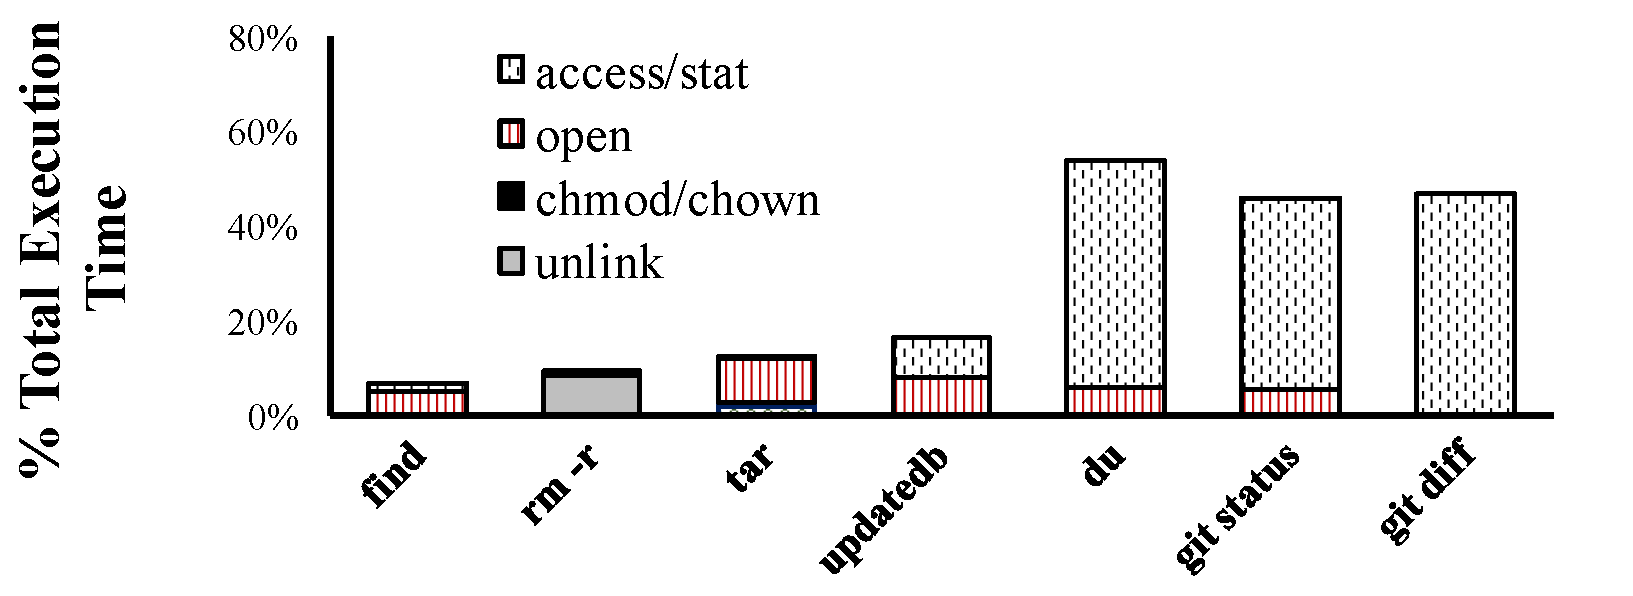
\includegraphics[width=5in]{dcache/plots/syscall-percentage.pdf} \\
\caption[Fraction of execution time on path-based system calls.]
{Fraction of execution time in several common utilities spent
executing path-based system calls with a warm cache, as measured with ftrace.}
\label{fig:dcache:lookup-frac}
%\vspace{-10pt}
\end{figure}

%\fixmedp{Please check these \% against time.  I think git diff is too high.  git status seems ok.}

Directory caches are essential for good application performance.
%Unix was designed such that ``(almost) everything is a file'',
%thus even accesses to in-memory file systems, device files, FIFOs and domain sockets
%first pass through the directory cache.
%In other words, 
Many common system calls must operate on file paths,
which require a directory cache lookup.
For instance, between 10--20\% of all system calls in the iBench system call traces do a path lookup~\citep{filenotafile}. 
Figure~\ref{fig:dcache:lookup-frac} lists the fraction of total execution time
%, as well as system time, 
several common command-line applications spend executing path-based system calls
(more details on these applications and the test machine in \S\ref{sec:dcache:eval}).
We note that these system calls include work other than path lookup,
and that these numbers include some instrumentation overhead;
% are coarse measurements that include  and work than path lookup;
%, and includes some time 
%for synchronous I/O (e.g., during {\tt rename}) as well as non-path tasks (e.g., creating 
%a file handle as part of {\tt open});
nonetheless, in all cases except {\tt rm},
the system call times and counts are dominated by
{\tt stat} and {\tt open}, for which 
%can be serviced from cache and for which 
path lookup is a significant component of execution time.
For these applications, path-based system calls account for 6--54\% of total execution time.
%and 25--77\% of system time.  
This implies that
lowering path lookup latency is
 one of the  biggest 
opportunities for a kernel to improve these applications' execution time.




\begin{figure}[t!]
\centering
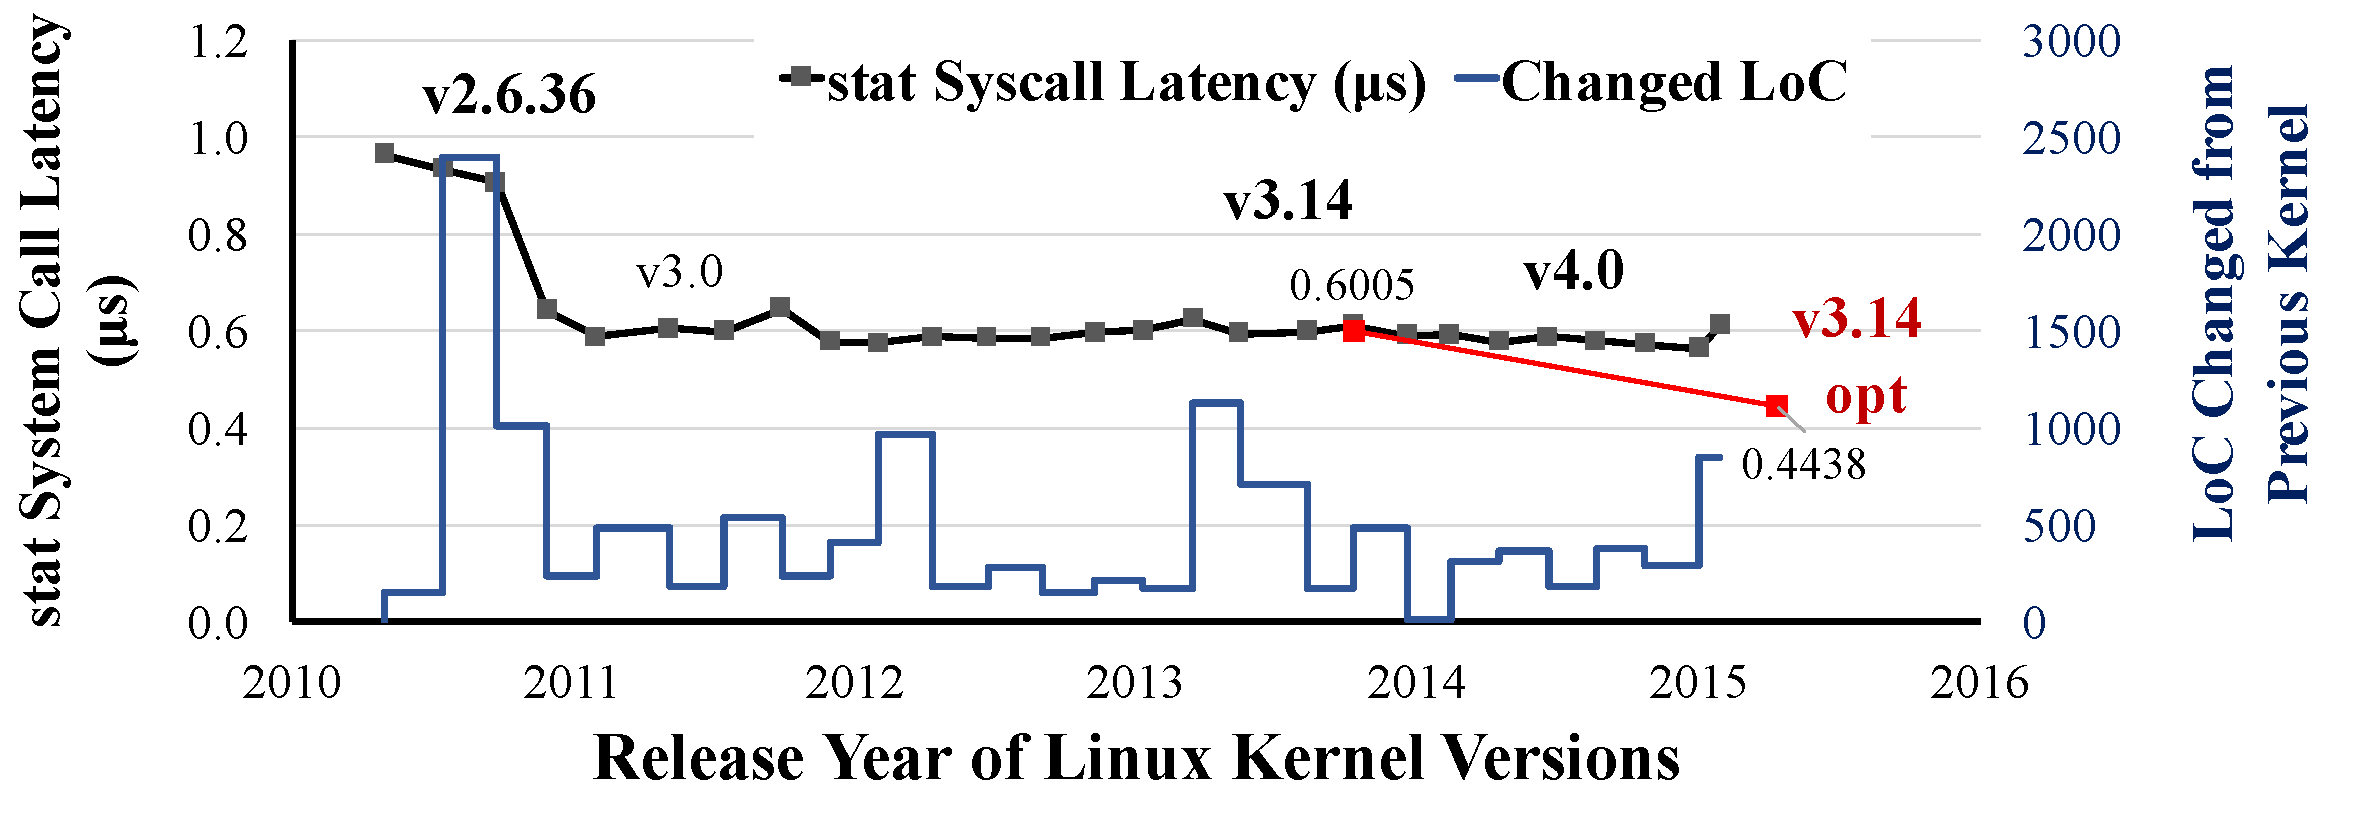
\includegraphics[width=6in]{dcache/plots/latency-by-version.pdf}
\footnotesize
\caption[Lantecy of {\tt stat} system call over years.]
{Latency of {\tt stat} system call with a long path {\tt XXX/YYY/ZZZ/AAA/BBB/CCC/DDD/FFF} on Linux over four years (lower is better), as well as the churn within the directory cache code (all insertions in {\tt dcache.c}, {\tt dcache.h}, {\tt namei.c}, {\tt namei.h} and {\tt namespace.c}). 
%Our optimizations significantly improve performance that has otherwise plateaued, despite significant ongoing developer effort.  
Our optimized \linuxver{} kernel 
further reduces {\tt stat} system call latency by \statspeedup{}\%.}
%\vspace{-15pt}
\label{fig:dcache:by-version}
\end{figure}


%\fixmedp{Add more evidence of lookup importance here: For instance, fraction of lookup time in file-related syscalls, or total lookup time in applications bound on file lookup latency.  }
Unfortunately, even directory cache hits are costly---0.3--1.1 \us{} for a {\tt stat} on our test Linux system, compared to only .04 $\mu$s for a {\tt getppid} and 0.3 \us{} for a 4 KB {\tt pread}. 
%\fixmetsai{Don, check this, I think read will be a better example, getppid is too trivial.}
This issue is taken particularly seriously in the Linux kernel community, which has 
made substantial revisions and increasingly elaborate optimizations to reduce the hit cost
of its directory cache, such as removing locks from the read path or replacing lock ordering with deadlock avoidance in a retry loop~\citep{corbet09jls,dcache-rcu}.
Figure~\ref{fig:dcache:by-version} plots directory cache hit latency against  lines of directory cache code changed 
over several versions of Linux, using a path-to-inode lookup \microbench{} on the test system described
in \S~\ref{sec:dcache:eval}.
These efforts have improved hit latency by 47\% from 2011 to 2013, but have plateaued
for the last three years.
%\fixmedp{if time, filter irrelevant changes from code deltas}
%at the cost of substantial developer effort.
%This latency appears to have plateaued 

The root of the problem is that the POSIX path permission semantics
seemingly require work that is linear in the number of path components,
and severely limit the kernel developer's implementation options.
%The root of this problem is that current directory cache
%designs reflect a straightforward implementation of the POSIX specification,
%which would seemingly require work that is linear in the number of path components.
For instance, in order to open file {\tt /\fnone{}/\fntwo{}/\fnthree{}} 
%for reading, 
one must have search permission
to parent directories {\tt /}, {\tt /\fnone{}}, and {\tt /\fnone{}/\fntwo{}},
as well as permission to access file {\tt \fnthree{}}.
The Linux implementation %of this specification is straightforward, 
simply walks the directory
tree top-down to check permissions.  
Unfortunately, when the critical path is dominated by 
walking a pointer-based data structure, 
including memory barriers on some architectures for multi-core consistency, 
modern CPUs end up stalling on hard-to-prefetch loads.
Moreover, because so many Linux features are built around this behavior, such as Linux Security Modules (LSMs)~\citep{wright+lsm},
namespaces, and mount aliases, it is not clear that any data-structural enhancements
are possible without breaking backward-compatibility with other Linux kernel features.
A priori, it is not obvious that a faster lookup algorithm, such as a single hash table lookup, 
can meet these API specifications and kernel-internal requirements; to our knowledge,
no one has tried previously.

%This paper proposes a decomposition of the directory cache, which allows
%most lookup operations to execute with a single hash table lookup (\S\ref{sec:dcache:dcache}),
%as well as optimizations to reduce the miss rate based on information that is {\em already in the cache}, but not used effectively (\S\ref{sec:dcache:readdir}).
%Our design maintains compatibility (\S\ref{sec:dcache:generalize}) through 
%several essential insights, including 
%how to separate the indexing of paths from checking parent permissions,
%and how to effectively and safely memoize the results of access control checks.


%% This paper proposes several new ways to organize a directory cache, which can yield 
%% substantial performance improvements over the current state of the art.
%% %This paper demonstrates that, despite this developer effort, there is still a substantial 
%% %missed opportunity hiding behind historical, intuitive, but not fundamental design choices.
%% Most of the Linux directory cache design reflects a straightforward implementation of the POSIX 
%% specification. %, with a division of labor that is suitable for mainstream file systems.

%This paper presents an alternative directory cache organization, which 
%improves performance by separating logical tasks, such as separating path indexing from permission checking; yet the design is sufficient to retain compatibility with POSIX.
%In the case of path lookup, 
%this paper demonstrates how 
%a per-component tree walk can be replaced with a single hash table lookup (\S\ref{sec:dcache:dcache}).
% without violating POSIX compliance.

%Our optimizations improve the performance of frequent lookup operations, but 
%introduce several costs, described in \S\ref{sec:dcache:dcache} and measured in \S\ref{sec:dcache:eval},
%which  we believe are acceptable and a net improvement for applications.
%First, these optimizations slow down infrequent modifications to the directory hierarchy, such as {\tt rename}, {\tt chmod},
% and {\tt chown} of a directory. 
%However, these slower operations
%account for less than .01\% of the system calls in the iBench traces~\citep{filenotafile}.
%Second,  the memory overheads of the dcache are increased.
%%(45\% per \dentry{}, as well as some  in our prototype).
%%(\fixmedp{XX MB} in our tests).  
%Third, lookup has a 
%probability of error from signature collisions that can be adjusted to be negligible
%%($2^{-141}$ in our configuration), 
%and within acceptable thresholds widely used by data deduplication systems~\citep{Debnath:2010:CSU:1855840.1855856, Srinivasan:2012:ILI:2208461.2208485, Quinlan:2002:VNA:645371.651321, Zhu:2008:ADB:1364813.1364831}.
%%, as well as how to remove
%%all memory barriers from the lookup path (\S\ref{sec:dcache:update}).
%In the micro-benchmark of Figure~\ref{fig:dcache:by-version}, our directory cache 
%optimizations improve lookup latency by 
%%revisions improve latency of accessing a long path
%%by 
%\statspeedup{}\% over unmodified Linux.
%%Our design addresses other missed
%%opportunities, such as identifying new opportunities to reduce the miss rate
%%through caching directory completeness.
%%\fixmedp{Do we want to highlight LoC?  3K is more than anything in the graph} \fixmetsai{Probably just mention in the evaluation. It's a metric that we should provide, but it's not awfully interesting.}
%%The total lines of code changed are fewer than 3,000 out of \fixmedp{XX}.
%%\fixmedp{Can we get 
%%, yet changes fewer than 3,000 lines of code.

%% SOSP cut - kind of long-winded
\begin{comment}
This paper rethinks current Linux directory cache design choices in light of the following goals:
\begin{compactitem}
\item {\bf Minimize the cost of a cache hit.} (\S\ref{sec:dcache:dcache}).
This means maximizing the benefit of temporal locality for frequent operations,
while pushing extra work of consistency maintenance onto less frequent, already-expensive operations.
%such as handling cache miss or updating massive metadata,
%in order to improve very frequent operations.
\item {\bf Maintain legacy compatibility.} (\S\ref{sec:dcache:generalize}).  Unix path semantics are complex, required by applications, file systems, and security modules, frustrating otherwise straightforward optimizations.  However tempting it may be to redesign path behavior to facilitate caching, path operations must exhibit the same behavior, with lower latency.
\item {\bf Never miss the same request twice in quick succession.} (\S\ref{sec:dcache:readdir}).  A number of less-frequent operations, such as reading a directory or secure temporary file creation, always miss in the cache {\em even if enough information is in cache to satisfy the operation.}  
%Of course, infrequent accesses should still be subject to a cache replacement policy, such as LRU.
\end{compactitem}
%Although directory caches must implement more complex semantics than a hardware memory cache,
%these principles should seem familiar to the reader with a basic architecture background.
%sadly, the Linux directory cache design violates all three.
\end{comment}

%This paper introduces several techniques to improve the performance of a directory cache,
%This paper explains several practical directory cache optimizations,
This paper demonstrates that these techniques improve performance for applications that use the directory cache heavily,
and the harm is minimal to applications that do not benefit.
%and that the worst case \microbench{} is only 12\% slower within \fixmedp{XX}\% of unmodified Linux.
%Each optimization we describe improves performance in isolation, and all can be combined.
%These optimizations change very few lines of code, and are backward-compatible with 
%legacy applications.  
%These changes are encapsulated in the VFS---individual file systems do not have to change their code.
%This paper describes a  prototype of these improvements implemented in Linux \linuxver{}.
%\S~\ref{sec:dcache:background} explains that the directory cache structure of Mac OS X, FreeBSD, and Solaris 
%are sufficiently similar that these principles should generalize.
%we compare and contrast Linux's directory cache
%with Mac OS X, FreeBSD, and Solaris in \S\ref{sec:dcache:background}, and explain inline how each
%optimization could be generalized to these other OS kernels.





%% \item {\bf Modularization and stackability}:
%% Any changes or optimizations must be implemented as modules inside Linux's VFS,
%% and can be stacked on top of the original design or any future optimizations. 
%% \item {\bf Backward compatibility}:
%% Any changes or optimizations must maintain least requirement of modifying any
%% file systems.
%% \item {\bf Generalization to other OSes}: Any changes or optimizations must be portable to other OSes with reasonable effort and change of design.




%% \dcache{} is proven to be effective on improving storage performance.
%% Experiments shows that,
%% in a Linux 3.x kernel, a \dcache{} with a xxx\% hit rate can speed up
%% metadata lookup and fetching time by xxx times.
%% \fixmetsai{experiment result, Linux version, and fs specs here}
%% However, we observed that Linux maintainers have made
%% constant and non-trivial efforts to improve \dcache{} in the Linux kernel.
%% We studied all \dcache{}-related source files in the Linux kernel Git repository,
%% and discovered that maintainers have committed
%% on average xxx revisions per source files.

%% We tested metadata lookup time on primary \dcache{}-related revisions.
%% Most changes on \dcache{} system only create xxx\%-xxx\% speed-up
%% than their predecessor.
%% \fixmetsai{result and graph here}.
%% Moreover, improvement to \dcache{} is still work-in-progress
%% for Linux maintainers.
%% \fixmetsai{reference to threads for latest dcache discussions}. 
%% All the evidences show that,
%% despite of significant reduction of storage operations,
%% efficiency of \dcache{} system internally still remains as a concern.

%% We argue that the design of \dcache{} needs to be carefully re-examined,
%% to fundamentally identify any missed opportunities that
%% improve value of \dcache{}.
%% At a high level, most optimization works for \dcache{} are focused on
%% improving ``how to cache'',
%% but we want to also lay eyes on ``what to cache'',
%% to ensure any valuable information returned from file systems
%% be captured by \dcache{} system.

%The contributions of this paper are as follows:
%\begin{compactitem}
%\item A performance analysis of the costs of path lookup and the opportunities
%to improve cache hit latency.
%\item A directory cache design that improves path lookup latency with a combination of techniques, including:
%  \begin{compactitem}
%  \item Indexing the directory cache by full path, reducing average-case lookup from linear to constant in the number of path components.
%  \item A Prefix Check Cache (PCC) that separates permission checking from path caching.  The PCC memoizes permission checks, and is compatible with LSMs~\citep{wright+lsm}.
%  \item Reducing the cost of checking for hash bucket collisions with path signatures.
%  \end{compactitem}
%\item Identifying opportunities to leverage metadata the kernel already has to reduce miss rates, such as tracking whether a directory is completely in cache.
%\item Carefully addressing numerous, subtle edge cases that would frustrate rote application of these techniques, such as integration with symbolic links and Linux namespaces.
%\item A thorough evaluation of these optimizations.  For instance, our optimizations improve throughput
%of the Dovecot IMAP server by up to \dovecotspeedup\% and latency of 
%updatedb by up to \updatedbspeedup{}\%.
%%git version control system by up to 25\%.
%
%\end{compactitem}

\subsection{Stream I/O}
\label{sec:abi:streams}



\issuedone{1.2.a}{discuss resource management at host level (I/O)}
I/O is part of the foundation
of an OS, to allow an application to interact with
other machines, users, applications, or system software.
An OS typically supports three types of I/O:
%An application requires interaction with the world during its execution, using I/O devices.
%I/O is a common feature of almost every OSes.
%The typical I/O needed in an application
%can be catagorized into three types:
{\bf storage}, for externalizing data to a permanent store;
{\bf network}, for exchanging data with another machine over internet;
and {\bf RPC} (remote procedure call),
for connecting concurrent applications or processes.
An OS must contain features for all three types of I/O abstractions,
and manages the resources on I/O devices, such as hard drives and NICs (network interface controllers).
Therefore, unless an I/O device is virtualized and dedicated to
an application or a guest,
a host OS must take a major role in I/O management;
for the least, a host OS has to share the resources among multiple applications or guests,
and contain the drivers to interface with the I/O devices.




%externalizing data to outside of the machines (i.e., networking);
% (i.e., storage);
%and  (i.e., remote-procedure call).
%A modern OS may define several abstractions
%for each types of I/O; for example, a file in Linux can be read using several system calls,
%including \syscall{read}, \syscall{pread}, and \syscall{readv};
%RPC in Linux is based on multiple inter-process abstractions,
%including pipes, UNIX sockets, and signals.




\fixmedp{Perhaps you want to start with defining a single byte stream abstraction? And then talk about how different URIs leads to different subclasses?}
The basic I/O abstraction in the host ABI
is a simple byte stream.
A byte stream allows sending or receiving information over an I/O device
as a continuous byte sequence.
According the type of I/O, a byte stream is restructured as the I/O device demands;
for example, on a storage device,
a byte stream is logically stored as a sequential file,
but physically divided into blocks;
on a NIC, a byte stream is transfered as packets, and identified by IP address and port number bound to a network socket;
a RPC stream can be simply a FIFO (first-in-first-out),
which applications or processes use to pass messages.
The host ABI for I/O is similar to the API of a UNIX-style OS,
which treats ``everything as a file descriptor''
and allows utilizing different types of I/O devices through the same file system APIs, including \syscall{read} and \syscall{write}.
Managing I/O as byte streams simplifies the development of both the library OS and PALs.
%The host ABI includes \hostapis{} for single-flavored, stream-type I/O, similar to the API of a UNIX-style OS.
%In general, a UNIX-style OS
%follows the design where ,
%meaning that each I/O abstraction is encapsulated by the file system APIs, such as \syscall{read} and \syscall{write}, to send and receive data on a file, a network socket, or a FIFO (first-in-first-out).
%but categorizes into three types:
%{\bf network connections}, {\bf regular files}, and {\bf RPC streams}.


The host ABI identifies I/O streams by URIs (unified resource identifier).
%These I/O streams
%are created or connected using a URI (unified resource identifier),
A URI is a unique name which describes 
both the subclass of an I/O stream, and the information for locating or identifying an I/O stream on an I/O device or inside the host OS.
The subclass of an I/O stream is identified by the URI prefix,
a keyword that represents different types of I/O: ``\palkeyword{file:}'' for regular files; ``\palkeyword{tcp:}'' and ``\palkeyword{udp:}'' for network connections; and ``\code{pipe:}'' for RPC streams.
The rest of the URI represents an identifier of the I/O stream:
for example, a file can be identified by a path located in a hierachical file system;
a network connection can be identified by the socket address.
The URIs standardize the way of identifying I/O resources inside various host OSes.


%According to the prefix of URI,
%the PAL can create either a synchronous I/O stream (e.g., a file or a connected socket)
%or named I/O server (e.g., a listening TCP socket).
%Modern OSes contain several out-of-band or asynchronous I/O abstractions, to improve the latency or CPU idle time
%when polling I/O streams.
%Although using out-of-band or asynchronous I/O is beneficial for application performance,
%providing these I/O features can be challenging for a host.
%Therefore, in \graphene{}, the host ABI restricts I/O abstractions to only synchronous stream I/O.


\fixmedp{Define these semantics without a reference to POSIX, so that the document is self-contained.}
The \hostapis{} defined in the host ABI for I/O are as follows:
%The host ABI for stream I/O presents a simplified, {\b POSIX file system}.
%A POSIX file system
%encapsulates I/O abstractions,
%including files, sockets, pipes, and even character devices,
%in the file system API.
%The host ABI contains several functions
%which resemble the POSIX API:
\palcall{StreamOpen} creates or opens an I/O stream;
\palcall{StreamRead} and \palcall{StreamWrite}
send and receive data over an opened I/O stream;
%are similar to \syscall{open}, \syscall{read}, and \syscall{write} in behavior, with a simplified, explicit semantic;
\palcall{StreamMap} maps %a is equivalent to \syscall{mmap} with a \code{MAP\_FILE} flag, mapping
a regular file to the application's memory; %, for reading or writing data.
\palcall{StreamAttrQuery} and \palcall{StreamAttrQuerybyHandle}
retrieves the file metadata and I/O attributes;
%as \syscall{stat} and \syscall{fstat} do;
%The POSIX-style functions simplify the porting of the host ABI
%on hosts with a similar specification.
\palcall{StreamWaitForClient} blocks and creates an I/O stream for incoming network or RPC connection;
\palcall{StreamSetLength} truncates a regular file;
\palcall{StreamFlush} clears the I/O buffer inside the host OS.
The following sections will discuss these \hostapis{} in details.





\subsubsection*{Opening or creating an I/O stream}




\begin{paldef}
HANDLE StreamOpen (const char *stream_uri,
                   u16 access_flags, u16 share_flags,
                   u16 create_flags, u16 options);
\end{paldef}



\palcall{StreamOpen} opens an I/O stream, % for future operations,
according to a URI given by \palkeyword{stream_uri} as a string argument. % to identifies resources associated with the I/O stream. 
The specification of 
\palcall{StreamOpen} includes interpreting the URI prefixes and syntaxes of \palkeyword{stream_uri},
and allocating the associated resources in the host OS and on the I/O devices.
\fixmedp{The term ``Opaque pointer'' is useful here}
If \palcall{StreamOpen} succeeds, it returns a {\bf stream handle}.
A stream handle is stored by the guest as an identifier to the opened I/O stream.
A stream handle is an opauqe pointer, which means the guest should only reference it as an identifier, and never try to interpret the content.
On the other hand, if \palcall{StreamOpen} fails (e.g., invalid arguments or permission denied), it returns a null pointer with the failure reason delivered with an exception.
% A stream handle is similar to a file descriptor in the POSIX API,
%but defined as a pointer to a data structure containing the stream information.
%The internal structure of a stream handle is up to the I/O stream type and the implementation of each PAL;
%a library OS is supposed to reference a stream handle
%only as an identifier.


\fixmedp{Need a listing of all the values of flags}
Other arguments of \palcall{StreamOpen} specify the options for opening an I/O stream:

\begin{compactitem}

\item
\palkeyword{access_flags} specifies the access mode of the I/O stream, which can be either \palkeyword{RDONLY} (read-only), \palkeyword{WRONLY} (write-only), \palkeyword{APPEND} (append-only), and \palkeyword{RDWR} (readable-writable).
The first three access modes are only available
for regular files; if the opened stream is a network or RPC stream, the access mode is always \palkeyword{RDWR}.
The access modes specify the basic access permissions that an application can request when opening a file.
The access permissions are validated by the host OS, based on user configurations.
For example, a file configured as append-only for the running application can only be opened in the \palkeyword{APPEND} mode.

\item
\palkeyword{share_flags} specifies the permissions for sharing a regular file (ignored for other types of  I/O streams)
with other applications, either in \graphene{} or in the host OS.
\palkeyword{share_flags} can be a combination of six different values:
\palkeyword{OWNER_R}, \palkeyword{OWNER_W}, and \palkeyword{OWNER_X}
represent the permissions to be read, writed, and executed by the creater of the file;
\palkeyword{OTHER_R}, \palkeyword{OTHER_W}, and \palkeyword{OTHER_X}
represent the permissions to be read, writed, and executed by everyone else.
The permissions are externalized to the host file system; access modes given in future execution are validated against the permissions.

\item
\palkeyword{create_flags} specifies whether to create a regular file,
when it does not exist in the host file system.
If \palkeyword{create_flags} is given as \palkeyword{TRY_CREATE},
it creates the file no matter if the file exists.
If \palkeyword{create_flags} is given as \palkeyword{ALWAYS_CREATE},
it fails if the file already exists.

\item
\palkeyword{options} specifies a set of miscellaneous options to configure the opened I/O stream.
Currently \palcall{StreamOpen} only accepts one option: \palkeyword{NONBLOCK} specifies that the I/O stream will never block whenever the guest attempts to read or write data.
The nonblocking I/O option is necessary for performing asynchronous I/O in the guest, to overlap the blocking time of multiple streams by polling (using \palcall{ObjectsWaitAny}).

\end{compactitem}


%includes different syntaxes for interpreting the URI and the rest of arguments,
%and different behaviors for creating or opening an I/O stream,
%according to the URI prefixes.
%uses a URI (uniform resource identifier), for specifying the I/O stream.
%An URI identifies both the type of I/O and the distination or location of the I/O stream.
%The type of a I/O stream is determined by URI prefix.
According to the consecutive operations, \palcall{StreamOpen}
returns two types of handles: One type represents a simple byte stream;
the other type is a server handle, which can wait on remote clients to initiate handshakes
for creating a byte-stream connection.
A server handle can be bound as a network server or a RPC server.
Because a server handle is not a byte stream, it cannot be directly read or written,
but can be given to \palcall{ServerWaitForClient} to block and receive a client connection.
The host ABI includes the abstraction of creating server handles
because receiving client connections requires control at the TCP/IP layer
and allocating host resources,
which cannot be implemented in the guest unless
the network stack is virtualized.




\palcall{StreamOpen} accepts the following URI prefixes and syntaxes for creating a byte stream or a server handle:


\begin{compactitem}

\item \palkeyword{file:[path]} creates or opens a regular file on the host file system.
The opened file is located by a path---either an absolute path from the root of the host file system, 
or a relative path.
\fixmedp{Mention CWD is relative to where the app is launched from. It may also be worth noting that this is included for convenience, but there are some security risks to using relative paths.}
A relative path is located from the initial directory where the application is launched,
and will never change afterward.
\palcall{StreamOpen} accepts relative paths for the convenience of locating application files packaged and shipped together.
Note that there could be security concerns
that a relative path may collide with another absolute path, or be ambiguous if the path starts with a ``dot-dot'' (i.e., walking back a directory).
Fortunately, both cases can be checked by the guest, as long as
the initial directory is specified by the host.
%based on user configurations.

\item \palkeyword{tcp:[address]:[port]} or \palkeyword{udp:[address]:[port]} creates a TCP or UDP connection to a remote server,
based on the IPv4 or IPv6 address and port number of the remote end.
One a connection is created,
it will exists until it is torn down by both sides.

\item \palkeyword{tcp.srv:[address]:[port]} or \palkeyword{udp.srv:[address]:[port]} create a TCP or UDP server handle which can receive remote client connections.
A TCP or UDP server is bound on a IPv4 or IPv6 address and an idle port number.
If the specified port number is smaller than 1024,
it may require additional privilege from the host OS.

\item \palkeyword{pipe.srv:[name]} or \palkeyword{pipe:[name]} create a named RPC server or a connection to a RPC server.
The name of a RPC server is an arbitrary, unique string.
An RPC stream is an efficient way for passing messages between applications or processes
running on the same host,
compare with using a network stream locally.
An RPC stream is supposed to be low-latency, and can scale up to significantly
more concurrent connections
than the limitation on network streams.

%The stream can be either a server which awaits incoming connection from other processes,
%or a client to an existing server.

\end{compactitem}



%Besides the abstraction,
%\palcall{StreamOpen}
%also inherits similar definitions of function arguments,
%including \palkeyword{access_flags}, \palkeyword{share_flags}, \palkeyword{create_flags}, and \palkeyword{options},
%from the POSIX-style \syscall{open}.
%%also inherit similar meanings from the options of \syscall{open}.
%These arguments specify the access type, file permission, creation mode, and other miscellaneous options of the I/O streams:
%for example, the access type can be specified as readable or writable,
%and the creation mode can be either explicit or implicit.
%An important concern is the choice of file permission (specified by \palkeyword{share_flags}), since the host ABI does not expose user credentials
%from the host.
%Setting the file permission in the host
%is mostly a usability feature: 
%an application can run more smoothly if some file permissions are externalized.
%For example, a compilor can create an executable with the execution permission, so that the consecutive building script can run the executable.
%The host ABI also externalizes the file permission
%which specifies specify whether a file can be shared with other applications.


\palcall{StreamOpen} defines the scope of enforcing and configuring security isolation in the hosts.
%URIs for \palcall{StreamOpen} represent three types of 
The host ABI restricts the sharing of host resources
to type types of simple I/O streams (i.e., file, network, and RPC). 
Other host resources, such as threads and memory,
are local to each process, and thus can be isolated by dedicating the host resources.
%Restricting the shareable host resource to I/O streams simplifies
%the enforcement of security policies in the hosts.
Therefore, in the host ABI, \palcall{StreamOpen} is the only \hostapi{}
which requires permission checks in the hosts.
Moreover, a user can configure the policies of sharing I/O streams by
whitelisting the URIs that are permitted for an application.





\subsubsection*{Reading or writing an I/O stream}



\begin{paldef}
u64 StreamRead  (HANDLE stream_handle, u64 offset,
                 u64 size, void *buffer);
u64 StreamWrite (HANDLE stream_handle, u64 offset,
                 u64 size, const void *buffer);
\end{paldef}                   
              
\palcall{StreamRead} and \palcall{StreamWrite} synchronously
read and write data over an opened I/O stream.
Both \hostapis{} receive four arguments: a \palkeyword{stream_handle} for referencing the target I/O stream;
\palkeyword{offset} from the beginning of a regular file
(ignored if the stream is a network or RPC stream);
\palkeyword{size} for specifying how many bytes are expected to be read or written;
and finally, a \palkeyword{buffer} for storing the read or written data.
At success, the \hostapis{} return the number of bytes
actually being read or written.


     




%The host ABI features include synchronously reading and writing data over an I/O stream.
%The behavior of \palcall{StreamRead} and \palcall{StreamWrite} is slightly different between a file stream and other type of stream:
%when reading or writing a file stream, \palcall{StreamRead} and \palcall{StreamWrite} accesses the file at a specific offset from the beginning of the file;
%otherwise, when accessing a network or RPC stream,
%the argument \palkeyword{offset} is ignored, and thus the ABI works similar to \syscall{read} and \syscall{write}.



\palcall{StreamRead} and \palcall{StreamWrite} avoid the semantics of sequential file access
to skip the migration of stream handles.
A regular file opened by \palcall{StreamOpen} (not in the append-only mode)
can only be read or written at an absolute offset
from the beginning of the file.
The random file access prevents the host OSes to track the offset
as an internal state,
and allows a migrated guest to reopen the I/O stream on another host
without migrating the host OS states.
Because all the host OS states associated with an I/O stream is only meaningful to the host,
and can be receated anytime,
the I/O stream appears to be {\em stateless} to the guest.



%The design is to keep the stream handle stateless inside the PAL,
%for cleanly migrating a library OS.
%Since the library OS is responsible of maintaining the offset of a file descriptor,
%a library OS instance can be easily detach from a PAL,
%by simply ``invalidating'' a stream handle;
%the library OS should be able to always reopen the stream after migration,
%or after a failure of accessing a stream handle,
%to recover the state of an I/O stream.



The host ABI does not includes asynchronous I/O semantics, or peeking into network or RPC buffers inside the host OS.
%Another challenge in the library OS, regarding I/O streams,
%is to support asynchronously I/O, or peeping data received over a network or RPC stream.
%This design decision is made to keep the host ABI simple.
Asynchronous I/O and peeking the buffers are both
common OS features that an application may depend on.
Although the features are not included in the host ABI,
the guest (i.e., the \libos{}) is supposed to emulate these features using the synchronous \palcall{StreamRead} and \palcall{StreamWrite},
combined with other \hostapis{} (e.g., \palcall{ObjectsWaitAny})
to prevent blocking on an I/O stream.
The guest can also allocate its own buffer to store data prematurely received from an I/O stream,
to serve the buffer peeking feature.
More details of these features are discussed in Chapter~\ref{chap:libos}.

%To implement the full Linux I/O features,
%the library OS must emulate asynchronous I/O,
%using the synchronous
%\palcall{StreamRead} and \palcall{StreamWrite}.
%The emulation requires opening the I/O stream in a non-blocking mode,
%and polling the stream handle before reading or writing data.
%The library OS can also buffer the data being read or written over a stream,
%as long as the buffered state is coordinated over every processes
%which share the same stream.


\paragraph{Alternative.}
An alternative strategy is to define a host ABI with asynchronous I/O semantics.
An asynchronous read or write
does not return a result immediately; instead, it creates an event handle
which can be polled arbitrarily.
An ABI that asynchronously reads and writes an I/O stream
potentially has more predictable semantics,
because the guest can explicitly tell which \hostapis{} will be blocking.
This strategy
is taken by Bascule~\cite{baumann13bascule}.
\graphene{} chooses synchronous I/O over asynchronous I/O in the current host ABI,
because synchronous I/O is a more common feature in host OSes.


 


%Defining  \hostapis{} for asynchronous read and write
%may potentially sacrifice portability, \fixme{cites some host that doesn't have async IO}
%since asynchronous I/O is less common seen in OSes.
%However, 
%can potentially be a more flexible option for emulating other I/O features in the guest.
%For example, the guest can emulate a synchronous read by polling a stream followed by asynchronously reading it.



%An asynchronous I/O ABI can be potentially
%more flexible for implementing the library OS features,
%as it can emulate both synchronous and asynchronous behaviors
%without buffering.
%The only reason that we choose synchronous over asynchronous I/O
%in the host ABI is to reduce the porting effort,
%especially for a host which lacks
%asynchronous I/O features.



\subsubsection*{Mapping a file to memory}
                   
\begin{paldef}            
u64 StreamMap (HANDLE stream_handle, u64 expect_addr,
               u16 protect_flags, u64 offset, u64 size);
\end{paldef}


\palcall{StreamMap} maps a file stream to an address in memory, for reading and writing data, or executing code stored in a binary file.
\palcall{StreamMap} creates a memory region
as either a copy of the file,
or a pass-through mapping which shares file updates with other processes.
When calling \palcall{StreamMap},
the guest specifies an expected address in memory for mapping the file, or a null address (i.e., zero) for mapping at a random address decided by the host.
\palkeyword{expect_addr}, \palkeyword{offset}, and \palkeyword{size} have to be aligned
with the allocation granularity of the hosts (more discussion in Section~\ref{sec:abi:memory}).
\palkeyword{protect_flags} specifies the protection mode
of the memory mapping, as a combination of \palkeyword{READ} (readable), \palkeyword{WRITE} (writable), \palkeyword{EXEC} (executable), and \palkeyword{WRITE_COPY} (writable local copy).
At success, \palcall{StreamMap} returns the starting address of the mapped area; otherwise, a null address is returned.




The host ABI includes \palcall{StreamMap} for two reasons. First, memory-mapped I/O is suitable for certain file access patterns of applications, and cannot be fully emulated by the guest using \palcall{StreamRead} and \palcall{StreamWrite}.
An application often chooses memory-mapped I/O for
avoiding the overhead of memory copy and context switch, %, especially when the application contains
for frequent, small, random file reads and writes.
Second, memory-mapped I/O is asynchronous by nature.
The data written to a file-backed memory mapping can be lazily flushed out to the storage;
the same feature is difficult to emulate in the guest
%due to lack of ability to efficiently determine which pages are recently updated,
% and thus should be synchronized with the storage.
without an efficient way of marking recently-updated pages (page table dirty bits can only be accessed in host OSes).
%without access to dirty bits in the page table.




%However, the challenge to implementing this behavior
%is to externalize the latest file state
%written by the application,
%on a host which disallows file-backed memory.
%For example, in a SGX enclave, all memory will have to be private memory,
%to be individually encrypted by the CPU.
%For a host which doesn't support pass-through file mappings,
%\palcall{StreamMap}
%can only guarantee writing out
%the latest file state to the disk when the memory is unmapped, using \palcall{VirtMemFree}.


\fixmedp{there should be an explicit semantics about when the mapping is visible back to the host, like on a sync, with the option to flush earlier}
Although \palcall{StreamMap} allows multiple processes to map the same file into memory, it does not guarantee the data to be coherently shared across processes.
Because memory-mapped I/O is asynchronous,
the data written in the memory is only guaranteed to be flushed to the storage
when the memory mapping is unmapped.
Also, the host ABI drops the assumption of memory sharing, especially for an isolated environment like SGX.
It is optional for the host to flush earlier,
or to coherently share the memory across multiple processes.













\subsubsection*{Listening on a server}


\begin{paldef}
HANDLE ServerWaitforClient (HANDLE server_handle);
\end{paldef} 


\palcall{ServerWaitforClient} waits on a network or RPC server handle, %created with a URI that starts with \palkeyword{tcp.srv:}, \palkeyword{udp.srv:}, or \palkeyword{pipe.srv:},
to receive an incoming client connection.
%Besides the I/O streams which can be directly read or written,
%the host ABI also supports creation
%of I/O stream server, which can be
%connected from another process (to a RPC stream server), or another host (to a network server), as a client of the server.
A network or RPC server handle cannot be accessed by \palcall{StreamWrite} or \palcall{StreamRead};
instead, the host OS listens on the server handle,
and negotiates the handshakes for incoming connections.
Once a connection is fully established,
the host OS returns a client stream handle, which can be read or written as a simple byte stream.
Before any connection arrives, \palcall{ServerWaitforClient} blocks eternally.
if a connection arrives before the guest calls \palcall{ServerWaitforClient},
the host can optionally buffer the connection in a limited backlog; the maximal size of server backlogs is up to the user configurations. The host will drop incoming connections when the backlog is full.




%I/O stream server has to block until a client
%connects the server, using \palcall{StreamWaitForClient}.
%\palcall{StreamWaitForClient} will return a stream handle, which represents a connection with the client.
%Other implementation
%is up to the host: for example,
%the host may decide a maximal number of incoming connections to buffer.









\subsubsection*{File and stream attributes}

%The host ABI features also include retrieving the metadata of an I/O stream.
%The retrieval of metadata is not limited to files,
%but also network sockets and RPC streams. %, to query the information regarding the streams.
%An example of metadata is the address of a network stream;
%when an unbound network stream is created,
%the host will randomly bind the stream to a local, temporary port, for identifying the connection at the IP (internet protocol) level;
%the POSIX API
%reveals the local port number
%to the applications,
%using \syscall{getsockname}.
%Other stream metadata required by Linux or POSIX functionality
%includes the total bytes written over an I/O stream, and the permission to sharing an I/O stream with other applications.
%The host ABI includes two functions for querying stream metadata:

\begin{paldef}
bool StreamAttrQuerybyHandle (HANDLE stream_handle,
                              STREAM_ATTRS *attrs);
bool StreamAttrQuery (const char *stream_uri,
                      STREAM_ATTRS *attrs);

\end{paldef}

Both \palcall{StreamAttrQuerybyHandle} and \palcall{StreamAttrQuery} query the attributes of an I/O stream, and return the attributes in a \palkeyword{STREAM_ATTRS} data structure.
The only difference is that \palcall{StreamAttrQuerybyHandle} queries an opened stream handle,
whereas \palcall{StreamAttrQuery} queries a URI without opening the I/O stream.
\palcall{StreamAttrQuery} is convenient for querying stream attributes when the guest is not planning to access the data of an I/O stream.
%Because \palcall{StreamOpen} involves more operations in the host OS,
%\palcall{StreamAttrQuery} can quickly retrieve the attributes without actually opening the stream.
Both \hostapis{} return true or false for whether the stream attributes are retrieved successfully.



%Both functions fill out a data structure given by the library OS,
%with metadata regarding an I/O stream
%identified by either a stream handle or a URI.
%Keeping both functions can be convenient for the library OS to query a file without creating a stream handle;
%however, we can always consolidate the host ABI
%with only \palcall{StreamAttrQuerybyHandle},
%because \palcall{StreamAttrQuery} can be replaced by \palcall{StreamAttrQuerybyHandle}
%after \palcall{StreamOpen}.




\begin{paldef}
typedef struct {
    u16 stream_type, access_flags, share_flags, options;
    u64 stream_size;
    u64 recvbuf, recvtimeout;
    u64 sendbuf, sendtimeout;
    u64 lingertimeout;
    u16 network_options;
} STREAM_ATTRS;
\end{paldef}


The \palcall{STREAM_ATTRS} data structure consists of multiple fields specifying the attributes assigned to an I/O stream since creation.
\palkeyword{stream_type} specifies the type of I/O stream that the handle references to.
\palkeyword{access_flags}, \palkeyword{share_flags}, and \palkeyword{options} are the same attributes assigned to an I/O stream when the stream is created by \palcall{StreamOpen}.
\palkeyword{stream_size} has different meanings for files and network/RPC streams:
if the handle is a file, \palkeyword{stream_size} specifies the total size of the file;
if the handle is a network or RPC stream, \palkeyword{stream_size} specifies the size of pending data currently received and buffered in the host.


The remaining attributes are specific to network or RPC streams.
\palkeyword{recvbuf} and \palkeyword{sendbuf} specify the limitation of buffering the pending bytes, either inbound or outbound.
\palkeyword{recvtimeout} and \palkeyword{sendtimeout} specify the receiving or sending timeout (in microsends)
before a stream is considered being disconnected abruptly.
\palkeyword{lingertimeout} specify the timeout for closing or shutting down a connection
to wait for the pending outbound data.
\palkeyword{network_options} is a combination of flags that specify the options of configuring a network stream.
Currently \palkeyword{network_options} accepts the following generic options:
\palkeyword{KEEPALIVE} (enabling keep-alive messages), %\palkeyword{CORK} (don't send out partial data),
\palkeyword{TCP_NODELAY} (no delay on sending small data),
and \palkeyword{TCP_QUICKACK} (no delay on sending ACK responses).


\begin{paldef}
bool StreamAttrSetbyHandle (HANDLE stream_handle,
                            const STREAM_ATTRS *attrs);
\end{paldef}


\palcall{StreamAttrSetByHandle} is a \hostapi{} newly introduced by \graphene{}.
\palcall{StreamAttrSetByHandle} changes the attributes initially assigned to an I/O stream, and externalizes the change to the host OS.
\palcall{StreamAttrSetByHandle} is given an updated \palkeyword{STREAM_ATTRS} data structure,
which contains the new attributes to be assigned to the I/O stream.
\palkeyword{stream_type} cannot be changed, as well as any attributes that violate the limitation imposed by the host.


A dilemma for defining the \palkeyword{STREAM_ATTRS} data structure is
to decide which stream attributes,
especially for a network stream, should be exposed by the host,
A network stream attribute can be derived from an optional feature inside the host network stack,
or a configuration at the NIC level.
Exposing these stream attributes allows the guest to export APIs for applications
to fine-tune the I/O performance.
However, exposing too many attributes makes the host ABI
less portable on different host OSes, since these attributes may not have their equivalences in certain host OSes.
Eventually, a guest should not expect every attributes defined in \palkeyword{STREAM_ATTRS} to be always configurable,
and \palcall{StreamAttrSetByHandle} will raise a failure
if the guest tries to set an unavailable attribute.





%To complete the library OS implementation, \graphene{} introduces a new function,
%,
%for changing the metadata of an I/O stream.
%The main reason for changing metadata
%is to configure a network or RPC stream with several device-specific options,
%such as the number of lingering connections,
%or enabling the TCP keepalive feature.


%\subsubsection*{Truncating a file or flushing a stream}




%To externalize the change to an I/O stream, the library OS must ensure a file is truncated to the right length (\palcall{StreamSetLength}), or a network or RPC Stream has flushed the host buffer (\palcall{StreamFlush}).
%Both functions are private to a process; if multiple processes try
%to set the file length or flush a stream at the same time, one of the function calls may be ignored by the host.


\begin{paldef}
bool StreamSetLength (HANDLE stream_handle, u64 length);
\end{paldef}


Finally, \palcall{StreamSetLength} expands or truncates a file stream to a specific length.
In general, the data blocks on storage media are allocated dynamically
to a file when the file length grows.
If \palcall{StreamWrite} writes data beyond the end of a file, it automatically expands the file, by allocating new data blocks on the storage media.
However, a file-backed memory mapping created by \palcall{StreamMap}
lacks an explicit timing to expand the file
when writing to the memory mapped beyond the end of file.
\palcall{StreamSetLength} can explicitly request the host to expand a file to an appropriate length,
so that consecutive memory write will never raise memory faults.
\palcall{StreamSetLength} can also shrink a file to the actual data size
if the file has overallocated resources earlier.







%\subsection*{\graphene{}-specific stream I/O features}

%\begin{paldef}
%void StreamDelete (HANDLE stream_handle, uint direction);
%\end{paldef}


\paragraph{Listing a directory.}
\graphene{} extends the stream I/O feature in the host ABI to retrieve directory information.
A file system usually organizes files in directories,
and allows applications to retrieve a list of files in a given directory.
Instead of adding new \hostapis{} for directory operations,
the host ABI uses existing \hostapis{}, namely \palcall{StreamOpen} and \palcall{StreamRead},
for listing a directory.
When \palcall{StreamOpen} is given a file URI that points to a directory,
such as ``\code{file:/usr/bin}'',
\palcall{StreamOpen} returns a stream handle
which allows consecutive \palcall{StreamRead} calls to read the file list
as a simple stream.
The stream handle that references to a directory can only be read as FIFO (first-in-first-out),
and the returned data should contain a series of file names as null-terminated strings.
The stream handle cannot be written or mapped into memory.



%A POSIX file system contain a hierarchy of directories
%containing files and subdirectories.
%The file I/O in POSIX requires listing the entries in a directory;
%a POSIX function, \syscall{readdir}, returns a list of file and subdirectory names
%in a directory.
%In \graphene{}, we face a decision of whether to include directory I/O
%in the host ABI.
%An option is to maintain a local file in each directory
%to store a list of file and subdirectory names;
%however, this solution will requires maintaining the list whenever a new file or subdirectory is created.
%Therfore, we extend the host ABI,
%to allow opening a directory as a stream handle.
%The library OS can read a list of file and subdirectory names from a directory stream handle,
%generated by the hosts.




\paragraph{Character devices.}
The host ABI also supports reading or writing data over a character device, including a terminal.
A terminal can be connected as a stream handle,
using a special URI called \palkeyword{dev:tty}.
Other character devices include the debug stream of a process (the URI is \palkeyword{dev:debug}),
equivalent to writing to \code{stderr} in POSIX.





\subsection{Page management}
\label{sec:abi:memory}



%Linux applications 
%are generally developed and compiled under the assumption that the memory is managed
%by the OS with page-level granularity.
%%generally requires system API
%%for allocating, protecting, and deallocating memory at the same granularity.
%%A x86 application may require memory allocation to be strictly at the granularity of four-kilobyte pages,
%The primary Linux memory API,
%including \syscall{mmap}, \syscall{mprotect}, and \syscall{munmap},
%allows an application
%to arbitrarily create, modify, and destroy VMAs (virtual memory areas),
%wholly or partially,
%as long as the requested areas align to
%4KB.
%%Developers can avoid hard-coding the granularity in an application,
%%by retrieving the system setting using \syscall{getpagesize}.
%Specifically, the Linux dynamic loader (i.e., \code{ld.so}) %, an ubiqutous user-space component in Linux,
%uses \syscall{mmap} to map a binary file to a large memory area,
%and then divides the mapping into 4KB-aligned code and data segments.
%To implement the Linux memory API,
%the memory management scheme of the host ABI
%must be at least as fine-grained as 4KB pages.

\issuedone{1.2.a}{Discuss resource management at host level (pages)}
In the hos ABI, the abstraction for page management
is a {\bf virtaul memory area (VMA)}, a page-aligned, nonoverlaping region
in the guest's virtual address space.
A virtual memory area
specifies the memory region that requires the host OS to allocate the page resources,
either statically or dynamically.
There are two types of VMAs: one is a file-backed VMA, which is created by \palcall{StreamMap} and backs the memory pages with file data blocks.
The other type is an anoumous VMA, which is purely in DRAM and not backed by any files.
Either types of VMAs is part of the virtual address space,
and a VMA should never overlap with others created in the same virtual address space.
The host OS can choose to populate all the pages for a VMA immediately at creation of the VMA,
or delay the allocation until the first memory access (i.e., demand paging).






%The host ABI for memory management is as follows:
%\palcall{VirtMemAlloc} creates an anonymous, non-file memory mapping in a process, similar as \syscall{mmap};
%\palcall{VirtMemProtect} changes the read (R), write (W), or execution (X) permission in an address range;
%\palcall{VirtMemFree} frees the an address range.




\begin{paldef}
u64  VirtMemAlloc   (u64 expect_addr, u64 size, u16 protect_flags);
\end{paldef}


\palcall{VirtMemAlloc} creates an anonymous VMA in the guest memory. When \palcall{VirtMemAlloc} is given an expected address, the host OS must try to create the VMA at the exact address.
Otherwise, if no address is given, \palcall{VirtMemAlloc} can create the VMA at wherever the host OS sees fit, and does not overlap with existing VMAs.
Both \palkeyword{expect_addr} and \palkeyword{size}
must be page-aligned, and never exceed the permitted range in the guest's virtual address space.
\palkeyword{protect_flags} specifies the page protection in the created VMA, and can be given a combination of the following values: \palkeyword{READ}, \palkeyword{WRITE}, and \palkeyword{EXEC} (similar as \palcall{StreamMap} but without \palkeyword{WRITE_COPY}).
If \palcall{VirtMemAlloc} succeeds, it returns the starting address
of the created VMA, which the guest is permitted to access up to the given size.





\begin{paldef}
bool VirtMemFree    (u64 addr, u64 size);
bool VirtMemProtect (u64 addr, u64 size, u16 protect_flags);
\end{paldef}


\palcall{VirtMemFree} and \palcall{VirtMemProtect} modify one or more VMAs, 
by either freeing the pages
or adjusting the page protection in an address range.
Both \hostapis{} specify the starting address and size of the address range to modify;
the given address range must be page-aligned,
but can be any part of the guest virtual address apace,
and overlap with any VMAs, either file-backed or anonymous.
If the given address range overlaps with a VMA, the overlapped part is divided into a new VMA, and be destroyed or protected accordingly.


 



%The host ABI delegates physical memory management to the host. The division of labor between the library OS and the host is as follows:
%the library OS manages only the virtual memory layout of a process;
%the host is the one who decides the allocation of physical memory resources, among VMAs of all processes.
%The delegation avoids the competition between the host and guest
%on managing the physical memory, which is a common issue for virtualization.
%For example, a VM may suffer a problem called ``double-paging'' when both the host and guest is trying to swap unused pages out of memory; a VM needs to use techniques like ballooning~\cite{wldspurger02vmware-esx} to subtly coordinate with the host to make paging decisions,
%or use paravirtualization~\cite{vmware_vmi}.



\fixme{Moved from the beginning of this section}
The challenge to defining the host ABI for page management
is to accommodate different allocation models and granularities of the hosts.
A POSIX-style OS often assumes dynamic allocation with page granularity (normally with four-kilobyte pages);
the assumption is deeply ingrained in the design of page fault handler sand page table management
inside an OS like Linux or BSD;
the page management component in an OS
is usually low-level and closely interacting with the hardware interface,
to serve the needs of both the OS and applications.
Such an OS design makes it difficult to move page management
into the guest, unless using hardware virtualization such as
\fixmedp{Needs a cite, and probaly a more specific mention of what feature of VT you have in mind}
VT~\cite{VT}, which virtualizes page fault handlers and page table management to the guest.




\papersubsection{CPU scheduling}
\label{sec:abi:thread}

\issuedone{1.2.a}{Discuss resource management at host level (threading)}
The host ABI for CPU scheduling includes two abstractions:
creation of user threads, and scheduling primitives
for inter-thread synchronization and coordination.
%Both Linux and POSIX have defined a rich threading API, with various thread creation options
%and complex scheduling primitives.
%\graphene{} simplifies the host ABI
%by include only a small set of basic threading features.
%for each host to implement.
Threading in the host OS requires a CPU scheduler
to dynamically assign a non-blocking thread to an idle CPU core, until next epoch for scheduling.
The host OS usually implements one or several scheduling algorithms and also defines APIs for applications
to configure scheduler parameters.
The design of scheduling algorithms and
APIs is mostly idiosyncratic to each host OS,
and is difficult to find any common ground to define unified host ABIs that are portable on every host OSes.

%however, a host scheduler does have to ensure every thread to follow its expected behaviors,
%regardless of the scheduling algorithm.
%For the least, a host scheduler should avoid completely starving one of the living threads,
%so that the guest can make progress as expected.
%Other CPU scheduling criteria such as fairness, throughput, and CPU utilization
%are still critical to the application performance, but the host scheduler is responsible of improving these criteria.


As a compromise, \graphene{} focuses on defining host ABIs for CPU scheduling features
essential to application usability.
For instance, applications may depend on multiple threads to execute concurrently, either on different CPU cores or on the same CPU core with a time-sharing model.
Scheduling algorithms in the host OSes are generally expected to satisfy certain criteria, such as fairness, throughput, and reasonable CPU utilization.
As long as the host OSes have chosen
a general-purpose, maturely-implemented scheduling algorithm,
\thehostabi{} can omit features
for configuring scheduler parameters. 






\papersubsubsection{Creating or terminating a thread}



%Unlike a user thread in Linux or POSIX (i.e., a ``pthread''),
%a guest thread created by the host ABI,
%using \palcall{ThreadCreate},
%is simply a new context which starts at a function.
%The host ABI
%moves all the thread creation options,
%such as thread-local storage,
%to an initialization function called after the thread creation,
%inside the library OS.
%The purpose of \palcall{ThreadCreate}
%is simple: it creates a ``kernel thread'' in the host,
%which can be scheduled by the host scheduler,
%to run application code on another CPU core.
%The \graphene{} library OS does not implement its own scheduler.


\begin{paldef}
HANDLE ThreadCreate (void (*start) (void *), void *param);
\end{paldef}


\palcall{ThreadCreate} creates a host-level thread to be schedule by the host OS.
The parameters specify the initial state of a new thread, including the function to start thread execution and the parameter being passed to the function.
As soon as \palcall{ThreadCreate} successfully returns,
the caller thread and the new thread can be both scheduled by the host OS. %should both be live in the host OS.
%and scheduled to run in arbitrary order.
\palcall{ThreadCreate} returns a thread handle to reference the new thread in the caller.




To improve portability, \graphene{} simplifies
the definition of \palcall{ThreadCreate} in several ways.
First, \palcall{ThreadCreate} does not accept additional parameter for specifying
an initial stack of the new thread.
The simplification helps porting \palcall{ThreadCreate}
on a host where a new thread cannot start
on an arbitrarily-assigned stack.
For instance, an \sgx{} enclave statically defines the stack address of each thread
to prevent the host OS from manipulating
enclave thread execution.
On most host OSes, a new thread created by \palcall{ThreadCreate} starts on a fixed-size stack, but the \libos{} can easily swap the stack with a much larger one.
Second, \palcall{ThreadCreate} takes no creation options
except a starting function and a parameter.
Every threads created by \palcall{ThreadCreate} should look identical to the host OS,
in order to keep the abstraction maximally portable
on various host options.



\begin{paldef}
void ThreadExit (void);
\end{paldef}

\palcall{ThreadExit} terminates the current thread. The \hostapi{} takes no argument, and should never return if it succeeds.
The purpose of \palcall{ThreadExit} is to free the resources allocated in the host OS
for the current thread, including the initial stack.




%The host ABI does not implement thread exiting notifications.
%When a guest thread is terminated using \palcall{ThreadExit}, the PAL destroys the correspondent kernel thread
%without notifying other threads.
%The design counts on the library OS to implement the Linux-style notifications,
%including
%sending a \code{SIGCHLD} signal,
%or triggering a parent-wakening futex.
% assigned by a child thread ID field given to  


\papersubsubsection{Scheduling a thread}

\Thehostabi{} defines several calls to interrupt a thread, either blocking or running,
or to allow a running thread to voluntarily give up CPU resources.
The purpose of these scheduling APIs is to prevent a thread from busily waiting for a specific condition,
such as a variable being set to specific value or a certain time in the future.
Busy-waiting wastes CPU cycles,
and can potentially block application execution
if the host OS
has no enough CPU cores to schedule each thread or does not
implement a time-slicing scheduling algorithm (e.g., round-robin).
%Although the guest delegates scheduling to the host scheduler, the guest can proactively request for scheduling to improve CPU throughput.



%Besides thread creation,
%the host ABI needs scheduling features to interrupt a thread execution,
%or yield the CPU.
%The concerns for including scheduling features
%in the host ABI
%is two-fold.
%The first concern is regarding compatibility;
%an application may be stuck in a busy-waiting loop, if the library OS lacks the ability to interrupt the execution when certain events occur.
%Specifically, \palcall{ThreadInterrupt} interrupts a thread using a thread handle
%returned by \palcall{ThreadCreat}.
%The second concern is regarding the CPU occupancy;
%if a thread does not forfeit the CPU when it stops making progress,
%the CPU can be wasted being idle.
%\palcall{ThreadDelay} and \palcall{ThreadYield}
%delays the current thread, until a period of time has passed, or the host scheduler re-schedules the thread to a CPU core.



\begin{paldef}
u64  ThreadDelay (u64 delay_microsec);
void ThreadYield (void);
\end{paldef}


\fixmedp{Define the semantics a bit more. When you do a delay, presumably wait at least that long; are theere any cases you can return early (e.g., EINTR)?}
\palcall{ThreadDelay} and \palcall{ThreadYield} suspend the current thread for rescheduling in the host OS.
\palcall{ThreadDelay} suspends the current thread
for the given timespan (\palkeyword{delay_microsec}, in microseconds).
If the thread is suspended successfully and rescheduled after expiration of the specified period,
\palcall{ThreadDelay} returns zero after resuming thread execution.
If the thread is rescheduled prematurely, due to interruption of other threads (using \palcall{ThreadInterrupt}),
\palcall{ThreadDelay} returns the remaining suspension time in microseconds.


\fixmedp{When you do a yield, under what conditions are you rescheduled?}
\palcall{ThreadYield} simply yields the execution of current thread, and the thread can be rescheduled immediately by the host OS.
By calling \palcall{ThreadYield}, a thread can requests for rescheduling when it expects
to wait for certain conditions.
When a thread calls \palcall{ThreadYield}, the host scheduler will suspend the current time slice of the thread,
and rerun the scheduling algorithm
to select a runnable thread (can be the same thread if there is no other competitor).



\begin{paldef}
void ThreadInterrupt (HANDLE thread_handle);
\end{paldef}



Introduced by \graphene{},
\palcall{ThreadInterrupt} interrupts a thread and forces the thread to enter an exception handler immediately.
The definition of \palcall{ThreadInterrupt} has two primary purposes.
First, \palcall{ThreadInterrupt} can interrupt a suspended thread, and force the thread to resume execution immediately.
Second, \palcall{ThreadInterrupt} can interrupt a running thread from an infinite waiting loop.
%so that the thread can instantaneously respond to a sudden event.
Without \palcall{ThreadInterrupt},
a running thread can only detect events at a certain ``checkpoint'' in the \libos{}.


The three abstractions defined for suspension and rescheduling
commonly exist on most host OSes, including Linux, \win{}, and \osx{}.
System APIs similar to
\palcall{ThreadDelay} and \palcall{ThreadYield}
can be found on all host OSes,
with slight but mitigable definition differences.
\palcall{ThreadInterrupt} can be implemented with signaling on a POSIX-style host OS,
or similar inter-thread communication
mechanisms on other OSes.







\paragraph{Scheduler parameters.}
\Thehostabi{} currently contains no APIs for the \libos{} to configure scheduler parameters in the host OS.
%the host scheduler.
Generally, Linux and other OSes allow applications to configure scheduling parameters,
such as scheduling priorities and policies,
to improve CPU utilization.
For simplicity,
\thehostabi{} delegates scheduling to the host scheduler,
and only allows host-level configuration for scheduler parameters.
As a result, the \libos{} cannot emulate any Linux system APIs for configuring scheduler parameters,
such as \syscall{sched\_setparam}.
%Similar to memory management, the host ABI delegates scheduling to the hosts.
%As the design and implementation of the scheduling policies
%differ from host to host,
%the library OS cannot implement all the Linux scheduling API and policies in the user space,
%unless the host ABI exposes a wide interface
%for configuring the host scheduler.



Luckily, scheduler parameters does not impact most applications targeted by \graphene{}.
In general, applications can progress without setting scheduling priorities or policies, but may suffer poor performance.
A rare exception is when
an application set the CPU affinity of two collaborating threads to ensure concurrent execution.
%The only exception is CPU affinity, as binding a thread to one or multiple CPU cores.
Between a producer thread and a consumer thread,
failing to schedule the threads on individual CPU cores may cause the threads to deadlock.
Consider the following scenario:
the consumer thread A may busily wait for the producer thread B to deliver a new job, but never yield the CPU to allow thread B to proceed its execution.
%wherein the consumer busily waits for the producer.
%Such a producer-consumer model requires the producer and consumer threads to be scheduled on different CPU cores, to prevent being deadlocked by the scheduler.
% when an application requires
%producer and consumer threads
%to be scheduled on different cores,
%or the application may be deadlocked and stop progressing.
%which continues to poll a work queue;
%in this producer-consumer scenario,
%the threads must run on different CPU cores, to prevent deadlocks.
We propose adding a \hostapi{} called \palcall{ThreadSetCPUAffinity}
to support binding a thread to CPU cores:

\begin{paldef}
bool ThreadSetCPUAffinity (u8 cpu_indexes[], u8 num);
\end{paldef}

\fixmedp{Explain how the arguments work}
\palcall{ThreadSetCPUAffinity} binds the current thread to a list of CPU cores, as specified in \palkeyword{cpu_indexes}.
\palkeyword{cpu_indexes} is an array of non-negative integers, which must be smaller than the total number of CPU cores (specified in the PAL control block).



\papersubsubsection{Scheduling primitives}


\Thehostabi{} defines two scheduling primitives for synchronization between threads: mutually-exclusive (mutex) locking and event waiting.
These scheduling primitives improve user-space synchronization
implemented by atomic instructions or compare-and-swap (CAS).
The primitives prevent a thread from spinning on a CPU core
until the state of a lock or an event
is atomically changed,
%The host-level scheduling primitives
%%can prevent a thread from spinning on a CPU core,
%%by requesting the host scheduler
%can avoid the spinning
by suspending the thread in the host OS.





%, for synchronizing the execution
%of several threads running in parallel.
%The host ABI must provide scheduling primitives,
%because locking cannot be reliably implemented in the user space;
%user-space locking
%cannot prevent a thread from being interrupted inside a critical section,
%and thus 
%causing the application to deadlock.
%Also, user-space locking must be implemented using the compare-and-exchange (\code{CMPXCHG}) instructions, which may not be available on every architectures.
%Therefore, by including the scheduling primitives in the host ABI,
%\graphene{} can encapsulate different kinds of scheduling options available on the hosts.



\begin{paldef}
HANDLE MutexCreate (void);
void   MutexUnlock (HANDLE mutex_handle);
\end{paldef}


\palcall{MutexCreate} creates a handle for a mutex lock.
A mutex lock enforces atomic execution in a critical section:
if multiple threads are competing over a mutex lock
before entering the critical section,
only one thread can proceed while other threads will block until the lock is released again.
\palcall{MutexUnlock} releases a mutex lock held
by the current thread.
To acquire a mutex lock,
a generic \hostapi{},
\palcall{ObjectsWaitAny} (defined later),
can be used to compete with other threads,
or wait for the lock release if the lock is held.



\begin{paldef}
HANDLE SynchronizationEventCreate (void);
HANDLE NotificationEventCreate    (void);
void   EventSet   (HANDLE event_handle);
void   EventClear (HANDLE event_handle);
\end{paldef}



%\graphene{} inherit most of the scheduling primitives
%from \drawbridge{}~\cite{porter11drawbridge}:
%{\bf semaphores} ensures the atomicity of a critical section;
%{\bf events} enforces the order of execution among multiple threads.
%The events created by the host ABI
%can be separated into synchronization events and notification events;
%the former is used by a producer thread, to wake a consumer thread
%blocking on a queue;
%the latter notifies the occurrence of a condition
%and prevent further blocking of threads.
%Both semaphores and events resemblance the abstractions provided by the \win{} API;
%we show that these scheduling primitives are also portable on other hosts, including Linux, BSD, and \sgx{}, using futexes or similar locking mechanisms.



\palcall{SynchronizationEventCreate} and \palcall{NotificationEventCreate} create two different types of events.
Any thread can use \palcall{EventSet} to signal an event.
Signaling a synchronization event wakes up exactly one waiting thread to continue its execution.
A synchronization event coordinates threads that cooperate as producers and consumers;
a producer thread can signal exactly one blocking consumer at a time.
On the other hand, a notification event stays signaled until another thread
manually resets the event using \palcall{EventClear}.
A notification event object can be used for notifying the occurrence of a one-time event,
such as the start or termination of an execution.
%Both types of events can be waited by a thread. %, using \palcall{ObjectsWaitAny}.
%The difference is that
%singaling a synchronization event
%wakes up at most one thread that are currently waiting for the event,
%whereas signaling a notification event stops any thread from
%further blocking on the event.
\palcall{ObjectsWaitAny}
is also used
to wait for event signaling.


%Synchronization events and notification events are designed for different purposes.
%A synchronization event can be used in a producer-consumer model, wherein a consumer thread can block until a producer thread signals the event.
%On the other hand, a notification event can be used for notifying the occurrence of a one-time event;
%for example, a thread calling \palcall{ThreadCreate} can use a notification event to block until a new thread is created and starts execution.

The definition of the two scheduling primitives
covers two typical types of synchronization behaviors.
A mutex enforces atomicity of a critical
execution section.
An event enforces dependency relationship between
threads.
Both primitives are easy to port on most host OSes;
the host ABI directly adopts the definition from the \win{} API, and can be easily implemented
on Linux or similar OSes using futexes or POSIX thread (pthread) APIs. 


\papersubsubsection{Waiting for scheduling events}


%The host ABI allows the library OS to poll one or several handles
%at the same time.
%The possible handles to poll include semaphores, synchronization or notification events,
%or I/O streams.
%Therefore, the host ABI
%introduces a function, \palcall{ObjectsWait}, similar to \syscall{poll} in POSIX,
%with a timeout option.



\begin{paldef}
HANDLE ObjectsWaitAny (HANDLE *handle_array,
                       u8 handle_num, u64 timeout);
\end{paldef}


\palcall{ObjectsWaitAny} blocks the current thread for specific events listed in
a handle array (specified by \palkeyword{handle_array} and \palkeyword{handle_num}).
A common usage of \palcall{ObjectsWaitAny}
is to block on a scheduling primitive,
such as a mutex lock or a notification event.
If a certain event happens on one of the listed handles
\palcall{ObjectsWaitAny} resumes thread execution
and returns the handle to the caller. 
\palcall{ObjectsWaitAny} can only block on exactly one mutex lock or event, but can wait on
multiple I/O events.
When waiting on I/O events,
\palcall{ObjectsWaitAny} blocks until one of the listed stream handles receives incoming data or connections,
or encounters failures such as I/O stream shutdown.

%For the least,
%\palcall{ObjectsWaitAny} allows a thread to
%wait until a mutex lock is released, or an event is signaled.
%Moreover, \palcall{ObjectsWaitAny} can be used to poll %for certain events
%an I/O stream handle,
%to wait for events such as arrival or delivery of data,
%a stream being shut down.
%\palcall{ObjectsWaitAny}

\palcall{ObjectsWaitAny} takes a \palkeyword{timeout} argument to prevent waiting for an event indefinitely.
If the timeout expires before any event occurs,
%the occurrence of any events related with the given handles,
\palcall{ObjectsWaitAny} stops blocking
and returns no handle (NULL).


\palcall{ObjectsWaitAny} can also be used for polling multiple stream handles, to wait for I/O events
such as receiving inbound data or sudden failure.
Unlike a mutex lock or an event object, a stream handle can be associated
with multiple I/O events.
Therefore, the host ABI introduces a \hostapi{}, \palcall{StreamGetEvent}, to create a stream event handle
that represents a specific I/O event of the given stream handle.
The definition of \palcall{StreamGetEvent} is inspired by Bascule~\cite{baumann13bascule}.


\begin{paldef}
HANDLE StreamGetEvent (HANDLE stream_handle, u16 event);
\end{paldef}


\fixmedp{Could you accomplish the smae thing by creating more than one handle for a network socket?}
\palcall{StreamGetEvent} receives a stream handle and a specific I/O event.
The \palkeyword{event} argument can be given
one of the following values:
\palkeyword{READ_READY}, for notifying that there are inbound data ready to be read;
\palkeyword{WRITE_READY}, for notifying
that a network connection is fully established
and ready to be written;
and \palkeyword{ERROR}, for notifying that certain failures occur on the stream.

%A challenge to implementing polling
%to differentiate the I/O events which can occur on a stream.
%When blocking on a network or RPC stream, an application needs to be notified
%about three types of events:
%establishment of the connection (i.e., becoming writable), arrival of messages (i.e., becoming readable), and shut-down of the connection;
%thus, the \graphene{} host ABI introduces a new function,
%\palcall{StreamGetEvent},
%to generate a handle identifying these I/O events of a stream,
%and can be polled by \palcall{ObjectsWait}.
%The design also keeps the definition of \palcall{ObjectsWait} simple:
%\palcall{ObjectsWait} should do nothing more than blocking on an array of handles,
%until one of the handles
%is wakened, or the call timeouts.


\papersubsubsection{Thread-local storage}


On some OSes, such as Linux and \win{}, applications require a thread-local storage (TLS)
to store thread-private variables or maintain a thread control block (TCB).
On \graphenearch{},
TLS is often referenced by one of the FS and GS segment registers,
to improve the performance of accessing any variable in the TLS.
%from all other threads.
%Retrieving or assigning the value of the FS/GS register
%is a privilege operation
%and must be performed in the host kernel.
As a convention of Linux, many Linux application executables
contain hard-coded access to TLS
using the FS register.
Since setting the value of the FS/GS registers is a privileged operations,
\thehostabi{} requires a call to enter the host kernel
and set the registers for referencing TLS.


%Because thread-local storage can be frequently accessed
%in an application,
%it would be inefficient to constantly
%enter the kernel for retrieving the TLS data.
%A common design is to occupy one of the thread-private registers
%to store a pointer to the thread-local storage;
%on \graphenearch{}, the FS register is commonly used to reference the thread-local storage.




\begin{paldef}
u64 SegmentRegisterAccess (u8 register, u64 value);
\end{paldef}




\Thehostabi{} introduces a \hostapi{}, \palcall{SegmentRegisterAccess}, for reading or writing the FS/GS register value.
The \palkeyword{register} argument can be either \palkeyword{WRITE_FS} or \palkeyword{WRITE_GS},
with the \palkeyword{value} argument
being a pointer that references to the TLS area.
Otherwise, the \palkeyword{register} argument
can be \palkeyword{READ_FS} or \palkeyword{READ_GS},
to retrieve the FS/GS register value.
On success, the \hostapi{} returns the current value of FS/GS register.



\issuedone{1.3.e}{Discuss the FS/GS limitation}
Unfortunately, the feasibility of implementing \palcall{SegmentRegisterAccess}
depends on the host OS.
%The implementation of \palcall{SegmentRegSet}
%depends the host system interfaces. 
%By default, reading or writing the value of the FS/GS registers is a privileged operation
%which can only be performed in ring 0.
Linux and similar OSes allow the usage of FS/GS register,
primarily because the FS register is heavily used in the standard C library.
%or BSD, the FS register is commonly used for bookkeeping in the standard C library;
%thus, the Linux or BSD system calls naturally include the feature of reading or writing the FS/GS registers in the kernel space (although only the FS register is used in the user space).
However, in other OSes, especially \win{} and \osx{},
changing the FS/GS register %is considered an unnecessary or even dangerous behavior,
is forbidden by the OS kernels.
The \win{} 7, 8, and 10 kernels confiscate the FS register for storing a thread control block (TCB),
and thus forbid users to change the FS register value.
\osx{}'s xnu kernel considers FS/GS registers to be of no concrete use.
These OS kernels
periodically reset the FS/GS registers
to mitigate any user attempt
of changing them.
If a host OS fails to implement \palcall{SegmentRegisterAccess},
the \libos{} may have to develop workarounds such as binary translation
to virtualize TLS access.


%we observe the case where changing the FS/GS registers is considered unnecessary and dangerous to the kernel.
%These hosts periodically reset the value of the FS/GS registers,
%preventing the host ABI to assign the TLS permanently.



%The primary challenge
%to implementing TLS for Linux applications
%is that an executable can hard-code the references to the FS register in its binary.
%Because a Linux executable is usually {\em unrelocatable},
%it can access a thread-private pointer by simply reading or writing to a specific offset
%to the FS register.
%To support these applications,
%a host must populate a valid TCB at the address pointed by the FS register;
%if the host forbids setting the FS register,
%the library OS cannot support TLS for an executable using thread-private pointers.

%On these hosts, the compatibility for TLS usage in applications is partially sacrificed.



\papersubsection{Processes}
\label{sec:abi:proc}


\fixmedp{don't mix perspective; focus in this chapter on the PAL model only. I would do minimal discussion of what the libOS does here.}
\Thehostabi{} creates clean, brand-new processes
for multi-process applications.
A process, or a {\bf picoprocess} in the perspective of the \libos{}, contains a new PAL instance,
a new \libos{},
and the application specified to \thehostabi{}.
\Thehostabi{} is designed to simplify porting a multi-process applications,
by dropping the assumption of
coherent memory sharing across processes.
Therefore, \thehostabi{} chooses a completely different process creation model
from the typical copy-on-write forking model
of UNIX-style OSes.

%The host ABI defines a process
%as a simple abstraction, which owns a new address space, and starts with a clean state of no guest VMAs, no held I/O resources, and no allocated handles.
%Moreover, a new process will not share any memory with former processes.
%The definition of the process abstraction
%is meant to simplify the host design for expanding a single-process execution to multiple processes.




%\graphene{} implements a distributed OS model for multi-process applications.
%Each process in \graphene{} has a library OS instance;
%Multiple library OS instances in a multi-process application must work together
%to present a single OS view,
%same as running in a native Linux.
%Therefore, the host ABI does not require copy-on-writing forking,
%but simply creation of a clean process instantiating the library OS.




\begin{paldef}
HANDLE ProcessCreate (const char *application_uri,
                      const char *manifest_uri,
                      const char **args, uint flags);
\end{paldef}


\palcall{ProcessCreate} creates a clean process to load an application executable specified by
\palkeyword{application_uri}. %, a URI that identifies the application executable.
\palcall{ProcessCreate} also allows specifying a manifest file (\palkeyword{manifest_uri}) for user policy configuration, as well as command-line arguments (\palkeyword{args}) passed to the new process.
\palcall{ProcessCreate} is equivalent to
relaunching the specified application in \graphene{},
except two distinctions: (1) \palcall{ProcessCreate} returns a process handle to its caller;
(2) a process created by \palcall{ProcessCreate} naturally belongs to the same {\em sandbox} as its parent.
%---an isolated container of related processes---with its parent process.
The detail of the sandbox abstraction is discussed in Section~\ref{sec:abi:proc:sandbox}.




%When creating a process, the host ABI, as \palcall{ProcessCreate}, takes a URI of the executable to run in the new process,
%together with a manifest file, which specifies the user policy.
%Once a new process is created, the library OS can be initialized
%and migrate the library OS and application state from the parent process;
%after migration, the new process can resume execution from the point of checkpointing,
%as a forked process.
%To the hosts, the processes in an application share nothing
%but the I/O streams opened by multiple processes.


%\palcall{ProcessCreate} returns a process handle.
%To bootstrap the inter-process communication, a process handle also works as an unnamed RPC stream connecting the parent and child processes.
%The guests in the parent and child processes can use this RPC stream to share internal states,
%as well as to inherit I/O stream handles from each other.

%The initialization of a library OS instance uses the RPC stream
%to retrieve namespace coordination information, such as how to locate the namespace leaders.
%The PRC stream is also used to send process migration data
%from the parent process, to implement forking.






\papersubsubsection{Sharing a handle}




Due to the statelessness of handles,
a guest can cleanly migrate its state to a new process, and recreate all handles afterward.
Unfortunately, not all I/O streams can be recreated
in a new process, due to the host limitations;
for instance, most host OSes bound network connections with the processes that first accept the connections,
and only allow sharing connections through inheriting
file descriptors from the parent process.
%is inherited through cloning.
%only identified by one handle or file descriptor,
%and can only be shared when the handle or file descriptor
%is inherited by a child process.
%The same inheritance feature also has to be implemented
%inside the library OS, to support Linux applications.
Since every process created by \palcall{ProcessCreate} is a clean picoprocess without inheriting any stream handles,
a guest needs a host feature
to share a network stream handle with other processes.


\begin{paldef}
void   RpcSendHandle (HANDLE rpc_handle, HANDLE cargo);
HANDLE RpcRecvHandle (HANDLE rpc_handle);
\end{paldef}



\Thehostabi{} introduces \palcall{RpcSendHandle} and \palcall{RpcRecvHandle} for sharing I/O stream handles over a RPC stream (a process handle is also used as a RPC stream).
\palcall{RpcSendHandle} 
migrates the host state of a stream handle, specified by \palkeyword{cargo},
over a RPC stream handle.
\palcall{RpcSendHandle},
which is called inside another process,
then receives the migrated host states from the RPC stream.
\palcall{RpcSendHandle}
will grant the receiving process permissions to access the I/O stream handle. % with the sending process.
If \palcall{RpcSendHandle} succeeds, it returns a handle
that references to the shared I/O stream.
The abstraction is similar to a feature in Linux and similar OSes that
shares file descriptors over a UNIX domain socket.

\papersubsubsection{Bulk IPC (physical memory store)}


%Migrating the guest state over a RPC stream can suffer significant overhead,
%when copying large chunks of memory.
%Especially, the RPC-based migration will slow down the
%latency of copy-on-write forking.
%the key overhead
%is caused by copying large chunk of memory
%across processes, without the help of a host to share the physical memory.



\Thehostabi{} introduces an optional bulk IPC feature, as a alternative to RPC streams.
The optimization brought
by the feature
is to reduce the latency of sending large chunks of data across processes.
The main abstraction of bulk IPC is a physical memory store.
Multiple processes can open the same memory store;
a processes sends the data in a piece of page-aligned memory to the store,
while another process maps the data to its memory.
Since the host can enable the copy-on-write sharing on the data mapped to both processes,
the latency can be much shorter than copying the data over a RPC stream.


%can send application memory to the physical memory store (using \palcall{PhysicalMemoryCommit}), which will keep a snapshot of the memory, set as copy-on-write.
%The child process can then attach to the physical memory store,
%and map the memory snapshot into its memory (using \palcall{PhysicalMemoryMap}).
%The Bulk IPC feature can large reduce the amount of physical memory copied during process migration,
%and thus optimize the latency of forking.


\begin{paldef}
HANDLE PhysicalMemoryStore  (u32 index);
\end{paldef}


\palcall{PhysicalMemoryStore} creates or attaches to a physical memory store,
based on a given index number.
The indexing of physical memory stores is independent for each sandbox (the container abstraction discussed in Section~\ref{sec:abi:proc:sandbox}),
so unrelated guests cannot share a physical memory store by specifying the same index number.
If \palcall{PhysicalMemoryStore} succeeds,
it returns a handle that references to the physical memory store.
The store is alive until every related processes close the corresponding store handles,
and no data is left in the store.




\begin{paldef}
u64 PhysicalMemoryCommit (HANDLE store_handle, u64 addr, u64 size);
u64 PhysicalMemoryMap    (HANDLE store_handle, u64 addr, u64 size,
                          u16 protect_flags);
\end{paldef}


\palcall{PhysicalMemoryCommit} commits the data in a memory range to a physical memory store.
Both \palkeyword{addr} and \palkeyword{size} must be aligned to pages,
so that the host can enable copy-on-write sharing if possible.
\palcall{PhysicalMemoryMap} maps the data from a physical memory store
to a memory range in the current process.
\palkeyword{protect_flags} specifies the page protection assigned to the mapped memory ranges.




\papersubsection{Sandboxing}
\label{sec:abi:proc:sandbox}


The security isolation of \graphene{} is based on a {\bf sandbox}, a container isolating a number of coordinating library OS instances.
When \graphene{} launches an application, the application begins running inside a standalone sandbox.
By default, a new process cloned by the application share the sandbox
with its parent process.
To configure the isolation policies,
developers provide a {\bf manifest} file for each application.
The policies are enforced by a reference monitor in the host.
A manifest file contains run-time rules for sandboxing resources which can be shared in the host,
including files, network sockets, and RPC streams.



Sandboxes delegate
enforcement of security isolation to the host OSes.
An application doesn't have to trust the library OS
to enforce security policies,
on every applications running on the same host.
If a library OS instance is compromised by the application,
the threat will be contained inside the sandbox,
and cannot cross the sandbox boundary, unless the host is also compromised.
For each sandbox,
the isolation policies are statically assigned,
in the manifest file given at the launch.
The isolation policies
cannot be subverted during execution.



\Thehostabi{} also introduces a \hostapi{}, \palcall{SandboxSetPolicy},
to dynamically move a process to a new sandbox.
Sometimes, an application needs to reassign the rules of security isolation,
for enforcing stricter rules inside the application.
A multi-sandbox environment can protect an application with multiple privilege levels, or an application that creates session for separating the processing for each client.
%belong to different sessions which should be isolated from each other.
With \palcall{SandboxSetPolicy}, a process that requires less security privilege
or serves a separate session can voluntarily moves itself to a new sandbox,
with stricter rules.
\palcall{SandboxSetPolicy} can dynamically
assign a new manifest file that specifies the new rules,
to be applied to the
new sandbox created for the current process.
%to restrict a process from accessing the resources shared by other processes.
%\palcall{SandboxSetPolicy}
%moves a process to a new sandbox.
%An option, \palkeyword{sandbox_rpc}, can block all RPC streams from other processes running in the original sandbox.







\begin{paldef}
bool SandboxSetPolicy (const char *manifest_uri,
                       u16 sandbox_flags);
\end{paldef}


\palcall{SandboxSetPolicy} receives a URI of the manifest file that specifies the sandboxing rules,
and an optional \palkeyword{sandbox_flags} argument.
The \palkeyword{sandbox_flags} argument currently can only contain one value:
\palkeyword{SANDBOX_RPC}, for isolating the RPC streams between the original sandbox and the new sandbox.

\subsection{Miscelleneous}
\label{sec:abi:misc}
%\papersection{Dynamic linking}
\label{sec:abi:linking}


\section{Manifests}
\label{sec:abi:manifests}
\section{Summary}
\label{sec:graphene:summary}

The \graphene{} design is centered around
building a para-virtualized layer, which can reuse the OS components for reproducing Linux system interfaces.
%instead of building arbitrary compatibility layers for reproducing the system interface.
%constantly porting the significant  of the existing system interface.
%In \graphene{}, 
\graphene{} defines a host ABI, as a new boundary between the OS and user space.
The host ABI is simple enough to port (containing \palcalls{} functions),
and exports sufficient functionality for virtualizing a primary part of the system API components.
A library OS is built upon the host ABI,
and implements \graphenesyscalls{} Linux system calls to reuse unmodified Linux applications.
\graphene{} decouples the development for a compatibility layer,
from host-specific challenges to building OS features, and isolating applications from other malicious tenants.



%\sysname{} extends library OS designs 
%to include multi-process APIs required by common applications, such as a shell or 
%web server.
%\sysname{} demonstrates efficient, selective
%coordination of shared state across multiple library OS 
%instances---maintaining host independence.
%%simplifying security sandboxing of otherwise unwieldy OS features.
%Applications on \sysname{} enjoy both 
%strong security isolation with acceptable performance and low memory overheads.
%% from unrelated programs 
%%and seamless shared namespaces 
%%among a group of coordinating guests.
%%% Although this paper focuses on distributed coordination
%%% to facilitate the efficiency benefits,
%%% expect our experiences with distributed coordination 
%%% may also be particularly relevant to highly scalable OS designs, 
%%% which avoid the bottlenecks of shared OS data structures~\cite{baumann09barrelfish, song11eurosys}.
%%Graphene's overheads are acceptable and the memory 
%%footprint is substantially lower than a VM.



%% , which could benefit from the reduced memory footprint
%% in a cloud 

%% by introducing a novel design for  coordination APIs. 
%% to a new OS (Linux),
%% new classes of applications,
%% and introduces a
%% %an alternative design point for storage virtualization.
%% Our results further demonstrate the feasibility of the library OS model.
%% % generally,
%% Applications on Graphene enjoy both 
%% strong security isolation from unrelated programs 
%% and seamless shared namespaces 
%% among a group of coordinating guests.
%% Although we explore this concept in a library OS,
%% we expect the namespace coordination framework 
%% could also be adapted to limit the attack surface area between
%% processes in a traditional OS.
%% We expect these experiences with distributed coordination 
%% may also be particularly relevant to highly scalable OS designs, 
%% which avoid the bottlenecks of shared OS data structures~\cite{baumann09barrelfish}.
%and specifically of content-addressable storage as the primary virtual storage abstraction.
%%% This work opens up a number of interesting questions for future work, 
%%% including studying opportunities for low-level storage optimization within the CAS server,
%%% making CAS the root file system,
%%% eliminating storage management in the host kernel, and 
%%% investigating the impact of frequent migration among devices.

\begin{comment}
Enabling legacy applications in a restricted environment,
such as \picoprocs{} or enclaves,
requires extra effort for mitigating the limitations of platforms,
in order to support typical OS personalities.
\graphene{}, as described in this chapter, extends the existing \libos{} designs
from isolating single-process or unshared abstractions
to include multi-process APIs required by many UNIX applications,
such as servers or shell scripts.
The challenge that \graphene{} primarily overcomes
is the requirement for coordinating shared states across multiple \picoprocs{},
to provides a collaborative, unified OS view.
Essentially, \graphene{} implements all shared, multi-process abstractions
and OS states
based on coordination over host-provided, pipe-like RPC streams.
The RPC-based, distributed OS implementation enables multi-process support in \graphene{}, with minimal extension to the host interface,
and a sweet-spot for enforcing inter-application security isolation,
by simply sandboxing the RPC streams.
Such a model largely reduces the complexity of
enforcing security isolation
on idiosyncratic multi-process abstractions
and shared states.
Because the corporative nature of \picoprocs{} in \graphene{},
an application can even dynamically impose sandboxing on one of its processes,
to reflect per-process, variable security policies.
\end{comment}

\begin{comment}
In principle, we attempt to use \graphene{} to justify the platform independence
of the \libos{} design,
without sacrificing its qualitative benefits,
such as isolating mutually-untrusting applications
and a narrow attack surface to kernels.
\graphene{} implements a considerable number of common Linux system calls,
to support popular, modern applications
such as Apache web server, GNU Make, OpenJDK \java{} VM and the Python runtime.
\graphene{} translates the high-level system APIs used by applications
to a host ABI
inherited and extended from a previous Windows-compatible \libos{}~\cite{porter11drawbridge}.
In addition, we port the \pal{} (Platform Adaption Layer) of \graphene{}
to various platforms,
including FreeBSD, OSX, Windows, and even a more restricted environment, the \intel{} \sgx{} enclaves.
In particular, \graphene{} being ported to \intel{} \sgx{}
(\graphenesgx{})
can isolate applications --- either single-process or multi-process
--- on a host where neither the operating system nor the hardware (except the CPU package)
is trusted by the applications. 
Overall, \graphene{} shows that,
by simply porting the reasonably sized host ABI
to a new platform,
a whole large spectrum of legacy applications tested on the previous platforms
can be activated all together.
\end{comment}

\makeatletter
\def\input@path{{}}
\makeatother
\graphicspath{{}}

\chapter{The Library OS}
\label{chap:libos}


\makeatletter
\def\input@path{{libos/}}
\makeatother
\graphicspath{{libos/figures/}}


%\section{Introduction}
%\label{sec:dcache:introduction}

Operating System kernels commonly cache file system data and metadata in 
a virtual file system (VFS) layer, which abstracts low-level file systems into a common API, 
such as POSIX.  
This caching layer has become a ubiquitous optimization
to hide access latency for 
persistent storage technologies, such as a local disk.
%whether a local disk or a network appliance, 
%have substantially higher access latencies than RAM,
%this caching layer 
%% SOSP Space - kind of quacking on
%% Caching
%% the file system directory hierarchy is particularly important because 
%% low-level file systems often spread this information across 
%% multiple disk sectors.
%% If an application wanted to open a single file on a system without a directory cache, 
%% most low-level file systems would issue numerous disk reads to locate the file and check the permissions
%% on the file and its parent directories;
%% a directory cache can commonly avoid these reads.
The directory cache is not exclusively a performance optimization; it also simplifies 
the implementation of {\tt mount}-ing multiple file systems, 
consistent file handle behavior,
and advanced security 
models, such as SELinux~\citep{selinux}.



%\fixmedp{Be charitable to developers, make our strong claims positively (we are really smarties) rather than calling them dummies}


%% Many observation shows that, in most systems, operations to storage are often
%% dominated by hierarchical structure traversal,
%% and fetching metadata of objects.\fixmetsai{references here}~\citep{duchamp94nfs}
%% In many file systems, traversal and metadata fetching
%% create random access patterns,
%% which are slower than sequential access patterns
%% on many storage media, e.g. magnetic disks.

% dp: I think this is getting down in the weeds.  We need to make the case for the work 
%     more strongly and generally first
%% Directory entry cache, a.k.a \dcache{},
%% is an important optimization in Linux kernels
%% to reduce storage operations for traversal and metadata fetching.
%% The design of \dcache{} is comparable to \vnode{} in BSD and \dnlc{} in Solaris.
%% \dcache{}, as well as \vnode{} and \dnlc{},
%% can be explained as a file system layer that
%% responds to requests on a cache hit,
%% but passes requests down to lower-leveled file systems on a cache miss~\citep{zadok06, skinner93}.

%\fixmedp{F1: Maybe thread together an argument about why no one would have tried a one-hop lookup before?}


%\marginpar{\scriptsize \textcolor{blue}{ Michael, I think the high-order bits are mostly right on Fig~\ref{fig:dcache:lookup-frac},
%but these number may change a bit as we refine the measurement}}

\begin{figure}[t]
\scriptsize
\centering
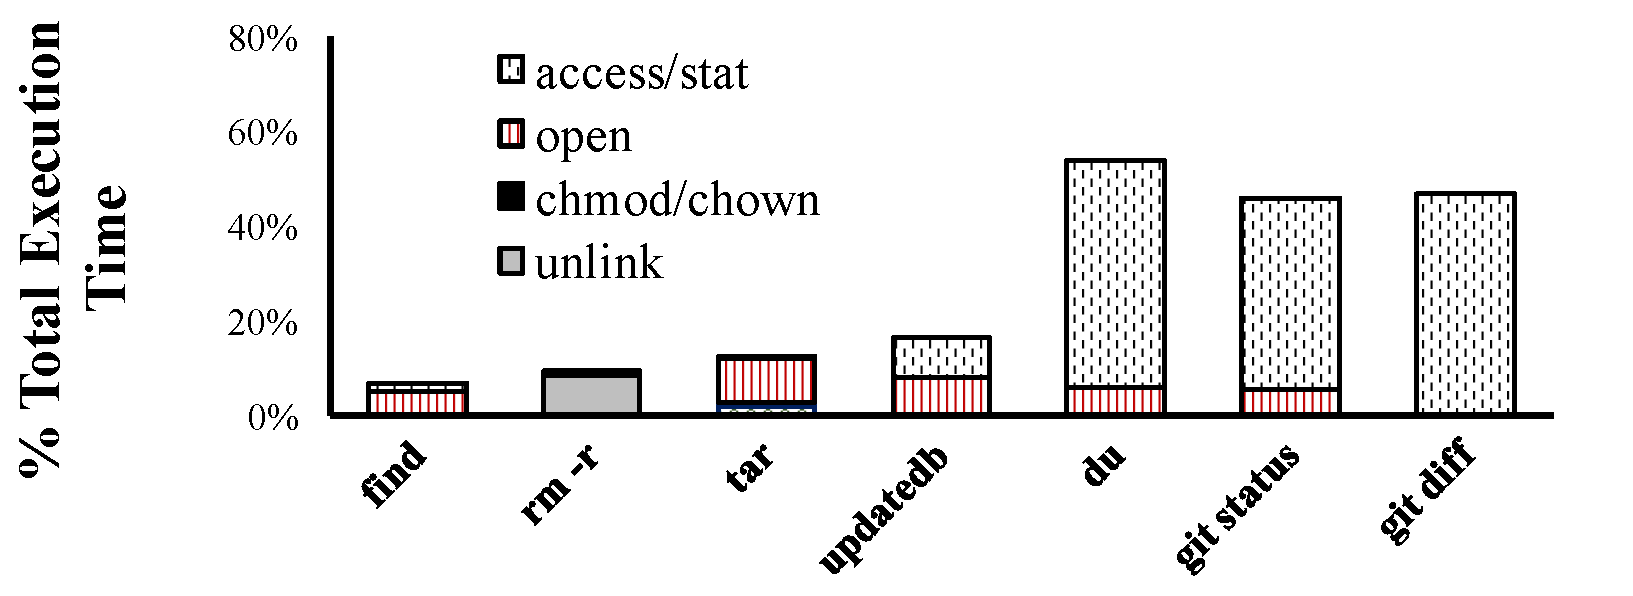
\includegraphics[width=5in]{dcache/plots/syscall-percentage.pdf} \\
\caption[Fraction of execution time on path-based system calls.]
{Fraction of execution time in several common utilities spent
executing path-based system calls with a warm cache, as measured with ftrace.}
\label{fig:dcache:lookup-frac}
%\vspace{-10pt}
\end{figure}

%\fixmedp{Please check these \% against time.  I think git diff is too high.  git status seems ok.}

Directory caches are essential for good application performance.
%Unix was designed such that ``(almost) everything is a file'',
%thus even accesses to in-memory file systems, device files, FIFOs and domain sockets
%first pass through the directory cache.
%In other words, 
Many common system calls must operate on file paths,
which require a directory cache lookup.
For instance, between 10--20\% of all system calls in the iBench system call traces do a path lookup~\citep{filenotafile}. 
Figure~\ref{fig:dcache:lookup-frac} lists the fraction of total execution time
%, as well as system time, 
several common command-line applications spend executing path-based system calls
(more details on these applications and the test machine in \S\ref{sec:dcache:eval}).
We note that these system calls include work other than path lookup,
and that these numbers include some instrumentation overhead;
% are coarse measurements that include  and work than path lookup;
%, and includes some time 
%for synchronous I/O (e.g., during {\tt rename}) as well as non-path tasks (e.g., creating 
%a file handle as part of {\tt open});
nonetheless, in all cases except {\tt rm},
the system call times and counts are dominated by
{\tt stat} and {\tt open}, for which 
%can be serviced from cache and for which 
path lookup is a significant component of execution time.
For these applications, path-based system calls account for 6--54\% of total execution time.
%and 25--77\% of system time.  
This implies that
lowering path lookup latency is
 one of the  biggest 
opportunities for a kernel to improve these applications' execution time.




\begin{figure}[t!]
\centering
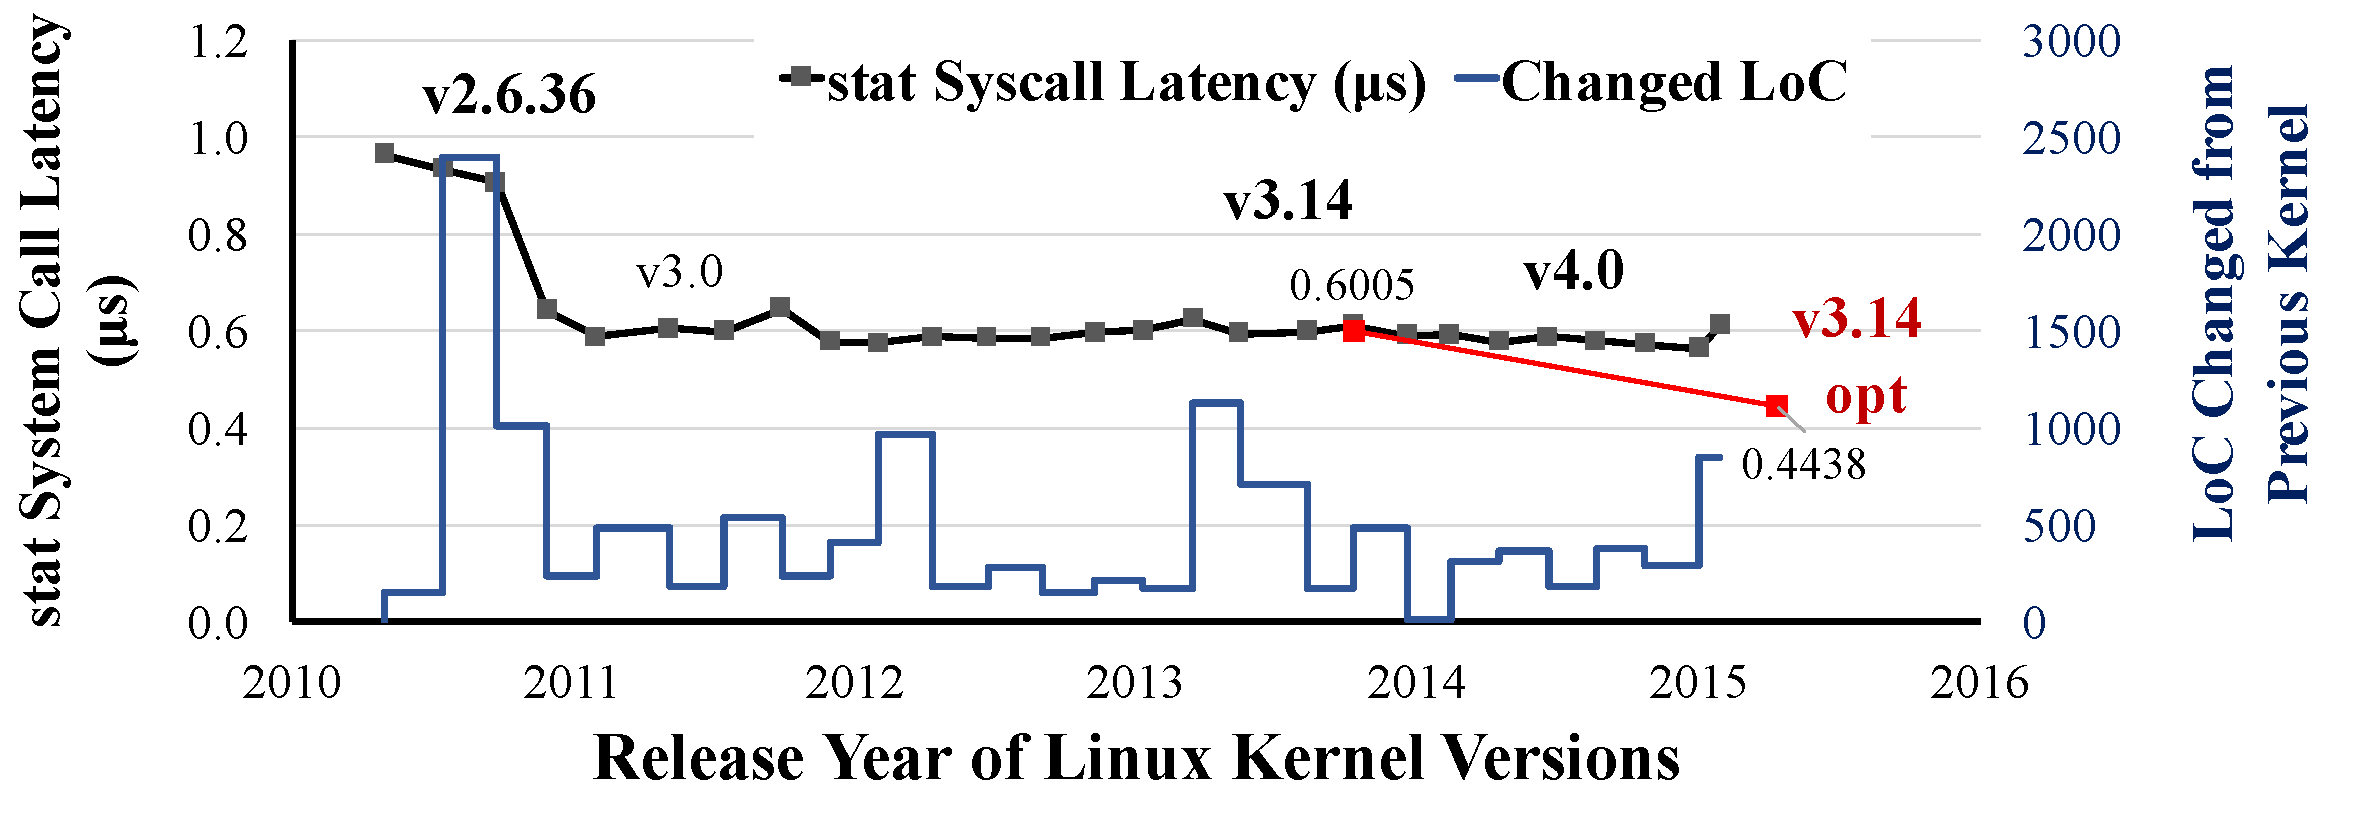
\includegraphics[width=6in]{dcache/plots/latency-by-version.pdf}
\footnotesize
\caption[Lantecy of {\tt stat} system call over years.]
{Latency of {\tt stat} system call with a long path {\tt XXX/YYY/ZZZ/AAA/BBB/CCC/DDD/FFF} on Linux over four years (lower is better), as well as the churn within the directory cache code (all insertions in {\tt dcache.c}, {\tt dcache.h}, {\tt namei.c}, {\tt namei.h} and {\tt namespace.c}). 
%Our optimizations significantly improve performance that has otherwise plateaued, despite significant ongoing developer effort.  
Our optimized \linuxver{} kernel 
further reduces {\tt stat} system call latency by \statspeedup{}\%.}
%\vspace{-15pt}
\label{fig:dcache:by-version}
\end{figure}


%\fixmedp{Add more evidence of lookup importance here: For instance, fraction of lookup time in file-related syscalls, or total lookup time in applications bound on file lookup latency.  }
Unfortunately, even directory cache hits are costly---0.3--1.1 \us{} for a {\tt stat} on our test Linux system, compared to only .04 $\mu$s for a {\tt getppid} and 0.3 \us{} for a 4 KB {\tt pread}. 
%\fixmetsai{Don, check this, I think read will be a better example, getppid is too trivial.}
This issue is taken particularly seriously in the Linux kernel community, which has 
made substantial revisions and increasingly elaborate optimizations to reduce the hit cost
of its directory cache, such as removing locks from the read path or replacing lock ordering with deadlock avoidance in a retry loop~\citep{corbet09jls,dcache-rcu}.
Figure~\ref{fig:dcache:by-version} plots directory cache hit latency against  lines of directory cache code changed 
over several versions of Linux, using a path-to-inode lookup \microbench{} on the test system described
in \S~\ref{sec:dcache:eval}.
These efforts have improved hit latency by 47\% from 2011 to 2013, but have plateaued
for the last three years.
%\fixmedp{if time, filter irrelevant changes from code deltas}
%at the cost of substantial developer effort.
%This latency appears to have plateaued 

The root of the problem is that the POSIX path permission semantics
seemingly require work that is linear in the number of path components,
and severely limit the kernel developer's implementation options.
%The root of this problem is that current directory cache
%designs reflect a straightforward implementation of the POSIX specification,
%which would seemingly require work that is linear in the number of path components.
For instance, in order to open file {\tt /\fnone{}/\fntwo{}/\fnthree{}} 
%for reading, 
one must have search permission
to parent directories {\tt /}, {\tt /\fnone{}}, and {\tt /\fnone{}/\fntwo{}},
as well as permission to access file {\tt \fnthree{}}.
The Linux implementation %of this specification is straightforward, 
simply walks the directory
tree top-down to check permissions.  
Unfortunately, when the critical path is dominated by 
walking a pointer-based data structure, 
including memory barriers on some architectures for multi-core consistency, 
modern CPUs end up stalling on hard-to-prefetch loads.
Moreover, because so many Linux features are built around this behavior, such as Linux Security Modules (LSMs)~\citep{wright+lsm},
namespaces, and mount aliases, it is not clear that any data-structural enhancements
are possible without breaking backward-compatibility with other Linux kernel features.
A priori, it is not obvious that a faster lookup algorithm, such as a single hash table lookup, 
can meet these API specifications and kernel-internal requirements; to our knowledge,
no one has tried previously.

%This paper proposes a decomposition of the directory cache, which allows
%most lookup operations to execute with a single hash table lookup (\S\ref{sec:dcache:dcache}),
%as well as optimizations to reduce the miss rate based on information that is {\em already in the cache}, but not used effectively (\S\ref{sec:dcache:readdir}).
%Our design maintains compatibility (\S\ref{sec:dcache:generalize}) through 
%several essential insights, including 
%how to separate the indexing of paths from checking parent permissions,
%and how to effectively and safely memoize the results of access control checks.


%% This paper proposes several new ways to organize a directory cache, which can yield 
%% substantial performance improvements over the current state of the art.
%% %This paper demonstrates that, despite this developer effort, there is still a substantial 
%% %missed opportunity hiding behind historical, intuitive, but not fundamental design choices.
%% Most of the Linux directory cache design reflects a straightforward implementation of the POSIX 
%% specification. %, with a division of labor that is suitable for mainstream file systems.

%This paper presents an alternative directory cache organization, which 
%improves performance by separating logical tasks, such as separating path indexing from permission checking; yet the design is sufficient to retain compatibility with POSIX.
%In the case of path lookup, 
%this paper demonstrates how 
%a per-component tree walk can be replaced with a single hash table lookup (\S\ref{sec:dcache:dcache}).
% without violating POSIX compliance.

%Our optimizations improve the performance of frequent lookup operations, but 
%introduce several costs, described in \S\ref{sec:dcache:dcache} and measured in \S\ref{sec:dcache:eval},
%which  we believe are acceptable and a net improvement for applications.
%First, these optimizations slow down infrequent modifications to the directory hierarchy, such as {\tt rename}, {\tt chmod},
% and {\tt chown} of a directory. 
%However, these slower operations
%account for less than .01\% of the system calls in the iBench traces~\citep{filenotafile}.
%Second,  the memory overheads of the dcache are increased.
%%(45\% per \dentry{}, as well as some  in our prototype).
%%(\fixmedp{XX MB} in our tests).  
%Third, lookup has a 
%probability of error from signature collisions that can be adjusted to be negligible
%%($2^{-141}$ in our configuration), 
%and within acceptable thresholds widely used by data deduplication systems~\citep{Debnath:2010:CSU:1855840.1855856, Srinivasan:2012:ILI:2208461.2208485, Quinlan:2002:VNA:645371.651321, Zhu:2008:ADB:1364813.1364831}.
%%, as well as how to remove
%%all memory barriers from the lookup path (\S\ref{sec:dcache:update}).
%In the micro-benchmark of Figure~\ref{fig:dcache:by-version}, our directory cache 
%optimizations improve lookup latency by 
%%revisions improve latency of accessing a long path
%%by 
%\statspeedup{}\% over unmodified Linux.
%%Our design addresses other missed
%%opportunities, such as identifying new opportunities to reduce the miss rate
%%through caching directory completeness.
%%\fixmedp{Do we want to highlight LoC?  3K is more than anything in the graph} \fixmetsai{Probably just mention in the evaluation. It's a metric that we should provide, but it's not awfully interesting.}
%%The total lines of code changed are fewer than 3,000 out of \fixmedp{XX}.
%%\fixmedp{Can we get 
%%, yet changes fewer than 3,000 lines of code.

%% SOSP cut - kind of long-winded
\begin{comment}
This paper rethinks current Linux directory cache design choices in light of the following goals:
\begin{compactitem}
\item {\bf Minimize the cost of a cache hit.} (\S\ref{sec:dcache:dcache}).
This means maximizing the benefit of temporal locality for frequent operations,
while pushing extra work of consistency maintenance onto less frequent, already-expensive operations.
%such as handling cache miss or updating massive metadata,
%in order to improve very frequent operations.
\item {\bf Maintain legacy compatibility.} (\S\ref{sec:dcache:generalize}).  Unix path semantics are complex, required by applications, file systems, and security modules, frustrating otherwise straightforward optimizations.  However tempting it may be to redesign path behavior to facilitate caching, path operations must exhibit the same behavior, with lower latency.
\item {\bf Never miss the same request twice in quick succession.} (\S\ref{sec:dcache:readdir}).  A number of less-frequent operations, such as reading a directory or secure temporary file creation, always miss in the cache {\em even if enough information is in cache to satisfy the operation.}  
%Of course, infrequent accesses should still be subject to a cache replacement policy, such as LRU.
\end{compactitem}
%Although directory caches must implement more complex semantics than a hardware memory cache,
%these principles should seem familiar to the reader with a basic architecture background.
%sadly, the Linux directory cache design violates all three.
\end{comment}

%This paper introduces several techniques to improve the performance of a directory cache,
%This paper explains several practical directory cache optimizations,
This paper demonstrates that these techniques improve performance for applications that use the directory cache heavily,
and the harm is minimal to applications that do not benefit.
%and that the worst case \microbench{} is only 12\% slower within \fixmedp{XX}\% of unmodified Linux.
%Each optimization we describe improves performance in isolation, and all can be combined.
%These optimizations change very few lines of code, and are backward-compatible with 
%legacy applications.  
%These changes are encapsulated in the VFS---individual file systems do not have to change their code.
%This paper describes a  prototype of these improvements implemented in Linux \linuxver{}.
%\S~\ref{sec:dcache:background} explains that the directory cache structure of Mac OS X, FreeBSD, and Solaris 
%are sufficiently similar that these principles should generalize.
%we compare and contrast Linux's directory cache
%with Mac OS X, FreeBSD, and Solaris in \S\ref{sec:dcache:background}, and explain inline how each
%optimization could be generalized to these other OS kernels.





%% \item {\bf Modularization and stackability}:
%% Any changes or optimizations must be implemented as modules inside Linux's VFS,
%% and can be stacked on top of the original design or any future optimizations. 
%% \item {\bf Backward compatibility}:
%% Any changes or optimizations must maintain least requirement of modifying any
%% file systems.
%% \item {\bf Generalization to other OSes}: Any changes or optimizations must be portable to other OSes with reasonable effort and change of design.




%% \dcache{} is proven to be effective on improving storage performance.
%% Experiments shows that,
%% in a Linux 3.x kernel, a \dcache{} with a xxx\% hit rate can speed up
%% metadata lookup and fetching time by xxx times.
%% \fixmetsai{experiment result, Linux version, and fs specs here}
%% However, we observed that Linux maintainers have made
%% constant and non-trivial efforts to improve \dcache{} in the Linux kernel.
%% We studied all \dcache{}-related source files in the Linux kernel Git repository,
%% and discovered that maintainers have committed
%% on average xxx revisions per source files.

%% We tested metadata lookup time on primary \dcache{}-related revisions.
%% Most changes on \dcache{} system only create xxx\%-xxx\% speed-up
%% than their predecessor.
%% \fixmetsai{result and graph here}.
%% Moreover, improvement to \dcache{} is still work-in-progress
%% for Linux maintainers.
%% \fixmetsai{reference to threads for latest dcache discussions}. 
%% All the evidences show that,
%% despite of significant reduction of storage operations,
%% efficiency of \dcache{} system internally still remains as a concern.

%% We argue that the design of \dcache{} needs to be carefully re-examined,
%% to fundamentally identify any missed opportunities that
%% improve value of \dcache{}.
%% At a high level, most optimization works for \dcache{} are focused on
%% improving ``how to cache'',
%% but we want to also lay eyes on ``what to cache'',
%% to ensure any valuable information returned from file systems
%% be captured by \dcache{} system.

%The contributions of this paper are as follows:
%\begin{compactitem}
%\item A performance analysis of the costs of path lookup and the opportunities
%to improve cache hit latency.
%\item A directory cache design that improves path lookup latency with a combination of techniques, including:
%  \begin{compactitem}
%  \item Indexing the directory cache by full path, reducing average-case lookup from linear to constant in the number of path components.
%  \item A Prefix Check Cache (PCC) that separates permission checking from path caching.  The PCC memoizes permission checks, and is compatible with LSMs~\citep{wright+lsm}.
%  \item Reducing the cost of checking for hash bucket collisions with path signatures.
%  \end{compactitem}
%\item Identifying opportunities to leverage metadata the kernel already has to reduce miss rates, such as tracking whether a directory is completely in cache.
%\item Carefully addressing numerous, subtle edge cases that would frustrate rote application of these techniques, such as integration with symbolic links and Linux namespaces.
%\item A thorough evaluation of these optimizations.  For instance, our optimizations improve throughput
%of the Dovecot IMAP server by up to \dovecotspeedup\% and latency of 
%updatedb by up to \updatedbspeedup{}\%.
%%git version control system by up to 25\%.
%
%\end{compactitem}

\section{The \thelibos{} Architecture}


The \libos{} of \graphene{}, or 
\thelibos{},
is a single library to be loaded beneath a Linux application,
as a compatible layer between
Linux \linuxapis{} and \thehostabi{}.
The purpose of \thelibos{} is to reuse an unmodified Linux application
upon an incompatible host OS or hardware.
%to support compatible OS features.
%for exporting compatible features.
An unmodified Linux application is built with the assumption of running on a Linux kernel or equivalent.
A Linux kernel
has exported a set of idiosyncratic features and characteristics,
or {\bf personality},
which an unmodified Linux application depends on.
%In order to reuse an unmodified Linux application
%on an incompatible host,
\thelibos{} takes the role of reproducing the Linux personality,
and is equivalent to a guest Linux kernel
over various host options.
%using \thehostabi{} exported by the host OS and PAL.
%The purpose of \thelibos{}
%is to resue an unmodified Linux application,
%by combining with a PAL and a host OS to behave as an equivalence of a Linux kernel. 
%%which is developed upon the assumption of running on a Linux kernel or equivalent.
%The main purpose of \thelibos{} is to reproduce
%the idiosyncratic features and behaviors of Linux,
%or the {\bf Linux personality},
%to resurrect Linux applications upon incompatible
%host OSes or hardware.
\graphene{} develops \thelibos{} as an ELF dynamic library (i.e., \code{\tt libLinux.so}),
loadable and linkable by a PAL.
%to be loaded on a host by the corresponding PAL.
%at the beginning of a \picoproc{}.


A key component of \thelibos{}
is a Linux system call table, which redirects \linuxapis{} from a Linux application to functions in \thelibos{}.
%a key Linux kernel component applications. 
%that \thelibos{} implements is the Linux system call table.
%For Linux and similar OSes,
A system call table is a primary entry point of a Linux kernel.
Each entry of the system call table
points to the kernel implementation of a Linux API related with a \linuxapi{} number (e.g., \code{NR\_open}).
%and triggers in-kernel operations for servicing requests from applications.
%and defines the interaction between applications and kernel.
\graphene{} moves the Linux system call table into \thelibos{},
and implements a number of \linuxapi{} handlers in the user space.
%The system call table in \thelibos{} contains a number of \linuxapi{} handlers,
Each \linuxapi{} handler emulates
individual \linuxapi{} that \graphene{} supports;
\graphene{} develops each handler
based on either a known specification, % known by the Linux application developers,
mostly described by a Linux manpage~\cite{linux-man-syscall},
or bug-for-bug behaviors
observed in a real Linux kernel.
For example, \syscall{rt\_sigaction} is partially documented
in the corresponding Linux manpage, and \thelibos{} implements the \linuxapi{} by mimicking the Linux kernel.
\graphene{} grows the functionality of \thelibos{}
primarily by extending the guest-level Linux system call table
with more complete \linuxapi{} implementation.

%Otherwise, for a few \linuxapis{} whose behaviors
%are not clearly defined by the Linux manpages,
%such as \syscall{rt\_sigaction},
%the \linuxapi{} handlers mimic the bug-for-bug behaviors of an actual Linux kernel.
%A continuing goal in \graphene{} is
%to extend \thelibos{} with more complete \linuxapi{} handlers.


%grow the functionality of \thelibos{},
%by extending the system call table with more complete handlers.




%The development of \linuxapi{} handlers in \thelibos{}
%is equivalent to implementing the specifications described in the Linux man pages~\cite{linux-man-syscall},
%including the valid inputs to each \linuxapi{},
%as well as the expected outcome.


%\paragraph{Implementing Linux Personality.} 
%\fixmedp{Revisit the logical flow of these paragraphs}
\Thelibos{} currently implements \graphenesyscallnum{} \linuxapis{},
and demonstrates 
the sufficiency of running applications ranging from servers to command-line applications.
For reference,
a relatively recent Linux kernel contains more than three hundred \linuxapis{}, including a long tail of infrequently-used \linuxapis{}.
%upon \thehostabi{}. % to interact with the host.
%Among the whole Linux \linuxapi{} table,
%A Linux kernel exports a long tail of infrequently-used \linuxapis{}.
%For reference, the Linux \linuxversion{} kernel exports \linuxsyscallnum{} \linuxapis{}.
A study of the Linux \linuxapi{} usage~\cite{tsai16apistudy}
indicates that only forty \linuxapis{} are indispensable to every applications available in the Ubuntu official repositories.
%The study also shows that
In the meantime, more than a hundred \linuxapis{} are used by only a single application,
or no application at all.
The development of \thelibos{} begins with
implementing twelve basic \linuxapis{} needed for running a ``hello world'' application,
such as \syscall{read}, \syscall{write}, and \syscall{open},
and then gradually grows the count of \linuxapis{}.
%for each new application introduced to run on \graphene{}.
As the count of \linuxapis{} continues to grow,
each time \thelibos{} is tested against a new application, the number of \linuxapis{} that need to be added
has dropped.
%Based on the types of applications priorized in \graphene{}, including servers, command-line programs, and language runtimes, some \linuxapis{} to be more important %for reusing the applications
%than the others. % \linuxapis{}.
According to the usage of each \linuxapi{} in applications,
developers can prioritize the popular \linuxapis{}, over other \linuxapis{} that are either unpopular among applications, or only used by administrative tools such as \code{reboot} or \code{ifconfig}.
\thelibos{} demonstrates that
\thehostabi{} is sufficient for implementing
a significant subset of the Linux \linuxapis{} to run
a representative sample of applications.


%The current \thelibos{} implementation
%includes a set of high-valued Linux \linuxapis{} for the types of applications
%that \graphene{} has targeted,
%including servers, command-line programs, and runtimes.
%The remaning \linuxapis{} may require extending \thehostabi{} with more privileged abstractions,
%including administrative operations
%and host-specific features.
%\thelibos{} demonstrates that \thehostabi{} is sufficient
%for exporting the host abstractions, to support a representative sample of Linux applications.

%such as memory sharing, scheduler configuration, and NUMA (non-uniform memory architecture) support.


%Linux exports a very long tail of infrequently-used \linuxapis{}.
%applications.




%An analysis indicates roughly 100 additional calls that can be implemented
%with the existing \pal{} ABI and coordination framework, less than 10 administrative calls that will not make sense to expose to 
%an application, such as loading a kernel module or rebooting the system, and roughly 54 that will require 
%\pal{} extensions to meaningfully implement, such as controlling scheduling,
%NUMA placement, I/O privilege, and shared memory.
%In the last category of system calls, the degree to which actual host details should be exported versus emulated is debatable.

%We believe represent the most commonly used system calls.
%When an application requests a call or argument that {\tt libLinux.so} does not implement,
%the picoprocess exits with a distinct error message. 
%Each time we have tested \graphene{} with a new application, the number of extra system calls
%required has dropped---most recently we only added 4 calls
%(namely, epoll\_create, epoll\_wait, semget and semop)
%to support the Apache web server.
%Thus, we believe \graphene{} implements a representative sample of Linux calls.

%such as {\tt sched\_setparam}, which manipulates scheduler-specific
%parameters or 
%{\tt uselib}, which has been abandoned 
%in {\tt glibc} version 2 in favor of a user-space dynamic linker.
%We do not plan to implement administrative interfaces, such as {\tt reboot}.
%The growth in the set of supported system calls has been driven by 
%the requirements of new applications we use to exercise \graphene{}, and has been 
%slowing considerably over time.



\subsection{\Linuxapi{} redirection}


\thelibos{} transparently intercepts \linuxapis{} in a Linux application. In a Linux kernel, a \linuxapi{} interrupt handler is assigned
to trigger the kernel operations,
whenever the application executes
a ``\assembly{syscall}'' or ``\assembly{int \$80}'' instruction.
The handler
performs a context switch from the application to kernel,
and redirects \linuxapi{} arguments to the kernel routine which services the requested \linuxapi{}.
%based on a kernel convention agreed by applications and Linux kernels.
\thelibos{} intercepts the \linuxapis{}
from an unmodified Linux executable or library, and redirects
to the system call table implemented inside \thelibos{}.
%intercepts the \linuxapis{}
%in an executable or library binary, and redirect the \linuxapis{}
%to the \linuxapi{} handlers inside \thelibos{}.
%\thelibos{} implements the callback functions for a subset of the Linux \linuxapis{}.
%For reference, Linux kernel \linuxversion{}
%has defined \linuxsyscallnum{} \linuxapis{} in total.


In normal cases,
\thelibos{} can redirect \linuxapis{} from an unmodified Linux application
using a modified C library (\libc{}).
%from an unmodified Linux application.
Most Linux executables and libraries avoid invoking \linuxapis{} directly,
but use \libc{} functions as wrappers to \linuxapis{}.
%which internally execute ``\code{syscall}'' or ``\code{int \$80}'' instructions.
%an executable or library in Linux and similar OSes invokes \linuxapis{} through \libc{},
%instead of directly containing the \code{syscall} instructions.
%The \libc{}
%contains a large set of \linuxapi{} wrappers,
%which encapsulate direct \linuxapis{} to the kernel as functions.
For example, the \libc{} function \funcname{read} is a wrapper to the \syscall{read} \linuxapi{},
which internally executes
the \assembly{syscall} instruction.
% that bares the same name and definition.
By defualt, \thelibos{} uses a modified
{\bf GNU C library (\glibc{})}~\cite{glibc},
since \glibc{} is compatible against most Linux applications released by Ubuntu. % are compatible against \glibc{}.
%which is compatible against most of the Linux applications released for Ubuntu.
%Other \libc{} variants, ,
%which are either fully or partially compatible with \glibc{},
%can be also modified to redirect \linuxapis{} to \thelibos{}.
%are alternatives upon \thelibos{} as long as they are modified for .
\graphene{} can also use other \libc{} variants,
such as \projname{uClibc}~\cite{uclibc} and \projname{musl}~\cite{musl},
if the application requires less \libc{} functionality.
%\graphene{} demonstrates that 
%are also demonstrated
%to be acceptable alternatives,
%with slight modification for \linuxapi{} redirection.




\graphene{} restricts the modification in \glibc{}
to up to \gipclines{} lines of code.
The C source code in \glibc{} consistently uses a platform-independent macro,
%referenced a single macro called
\funcname{INLINE\_SYSCALL},
to invoke \linuxapis{} to the kernel.
%when it needs to invoke a \linuxapi{}.
\funcname{INLINE\_SYSCALL} contains a piece of assembly code
that copies \linuxapi{} number and arguments to registers,
and then uses \assembly{syscall} to enter a Linux kernel.
\graphene{} modifies \funcname{INLINE\_SYSCALL}
to redirect a \linuxapi{} to
an entry point of \thelibos{} called \funcname{syscalldb}.
\funcname{syscalldb} saves the current register state, similar to a context switch,
and then
calls the \linuxapi{} handler
indicated by the \linuxapi{} number.
%, to trigger operations inside \thelibos{}.
For assembly code in \glibc{},
\graphene{} replaces each \code{syscall} instruction with
a dynamic call to
\funcname{syscalldb}, given the address of \funcname{syscalldb} is dynamically determined.
Figure~\ref{fig:libos:syscall-redirection} summarizes the mechanism of \linuxapi{} redirection.
%to \thelibos{}.


\begin{figure}[t!]
\centering
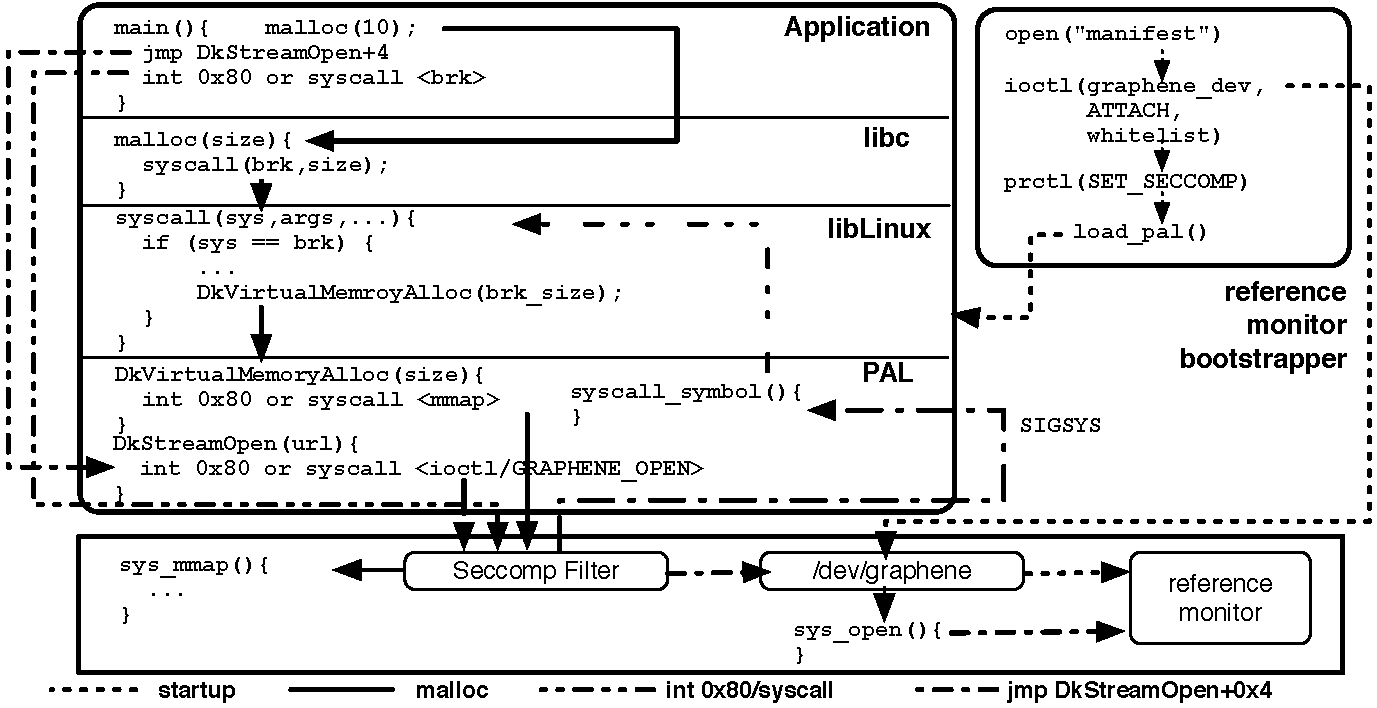
\includegraphics[width=\linewidth]{syscall-redirection.pdf}
\footnotesize
\caption{System call redirection for \thelibos{}.
In the normal case (first line of {\tt main}), {\tt malloc} is invoked causing the invocation of {\tt brk} ({\tt libLinux}) and {\tt mmap} in the \pal{}. In the second line, the application jumps to an address in \pal{}, which is permissible.
Files are accessed through {\tt ioctl} to {\tt /dev/graphene} and checked by reference monitor.
The third line invokes {\tt brk} with an {\tt int} instruction, which is redirected to the {\tt libLinux} function.}
\label{fig:libos:syscall-redirection}
\end{figure}


\graphene{} modifies several \glibc{} libraries with individual purposes,
%When using \graphene{}, an application must be deployed with the modified \libc{} libraries,
including \code{ld.so}, \code{libc.so}, \libpthread{}, and \libdl{}.
\Glibc{} partitions its code into separate libraries to reduce the binary sizes
loaded by each application.
%Despite that \glibc{} has partitioned its code into separate libraries,
\graphene{} only modifies the libraries which contains direct \linuxapis{} (i.e., \assembly{syscall} instructions).
%not every libraries of \glibc{} need to be modified for \linuxapi{} redirection.
%Only \code{libc.so}, \libpthread{}, and \libdl{} have included \code{syscall} instructions,
%and thus have to be modified for \graphene{}.
Other \libc{} libraries, such as \code{libm.so},
never directly invoke \linuxapis{} and only rely on 
existing \libc{} functions;
therefore, \graphene{} leaves \code{libm.so} and other similar \libc{} libraries unmodified.



\paragraph{Hard-coded \linuxapis{}.}
A static binary, or a platform-dependent application, may contain hard-coded \assembly{syscall} instructions
that cannot be redirected by a modified \libc{}.
Some application developers choose to statically link an executable against \libc{},
as a static binary with hard-coded \linuxapis{}. %\code{syscall} instructions.
Other application developers may program an application---usually a language runtime (e.g., go runtime) or system software (e.g., \projname{busybox})---with assembly code that directly invokes
platform-depenedent,
rare \linuxapis{} that are not wrapped by \libc{} functions.
%one of the \linuxapi{} wrappers in \libc{}, or \funcname{syscall}.
%As a result, a ELF binary may contain hard-coded \assembly{syscall} instructions.
%Either way leads to hard-coding \code{syscall} instructions in the ELF binaries.
Because modified \glibc{} does not redirect hard-coded \linuxapis{},
the \linuxapis{}
trigger context-switching into the host kernel,
causing security and compatibility issues as
exposing unauthorized, or unsynchronized host resources and states to the application.


As a solution,
\thelibos{} depends on host-level \linuxapi{} restriction to redirect hard-coded \linuxapis{}.
%to prevent \linuxapis{} from anywhere other than a PAL.
A direct \linuxapi{} traps into the host kernel,
unless the host has virtualized the interrupt handler to the \libos{}.
\graphene{} depends on each host to
detect unauthorized \linuxapis{} either from a wrong code location or with an unexpected \linuxapi{} number.
On Linux or a similar OS, the PAL can install a \linuxapi{} filter,
such as SECCOMP filter~\cite{seccomp}.
On some architecture, there are architectural limitation;
for example, SGX forbids \linuxapis{} inside an enclave and triggers an exception for an in-enclave \linuxapi{}.
%\code{syscall} instructions
%(e.g., SGX restriction).
%The details of the \linuxapi{} restriction mechanisms are discussed in
%\fixme{update labels}
%Section~\ref{sec:linux:syscall} and Section~\ref{sec:sgx:syscall}.
\thehostabi{} specifies that the host captures unauthorizes \linuxapis{}
and redirects to an exception handler (set up by \palcall{ExceptionSetHandler}).
%If a binary makes an illegal \linuxapi{},
%the host-level \linuxapi{} restriction will trigger an \code{ILLEGAL} exception
%at \thehostabi{},
%and thus the \linuxapi{} is redirected by an exception handler
%assigned by \thelibos{}.
The exception handler 
retrieves the \linuxapi{} number and arguments
from the saved context,
runs the \linuxapi{} handler,
and eventually pushes the return value back to the saved context. %\code{RAX} register.


Redirecting \linuxapis{} based on exceptions
can be expensive,
due to the overhead of context-switching between the host and guest.
Whenever an application invokes a direct \linuxapi{},
it traps into the host kernel, and then returns to the \libos{} to handle the \linuxapi{}.
Therefore, the process of redirecting a \linuxapi{} includes at least two times of context-switching, which can take up to microseconds.
To bypass the overhead,
\thelibos{} can 
rewrite the binary at run-time to redirect the hard-coded \linuxapis{};
%use {\bf binary translation} to modify the hard-coded \code{syscall} instructions;
\thelibos{} can
either scan-and-rewrites the whole binary at loading time,
or rewrites a single \assembly{SYSCALL} instruction in the exception handler.
%binary translation
%can be triggered when a host-level exception is raised
%for an illegal \linuxapi{},
%to optimize consecutive \linuxapi{} invocation at the same location.
%\thelibos{} can also perform a full scan in application binaries
%to spot and modify hard-code \code{syscall} instructions.
\graphene{} leaves the implementation of binary rewriting
as future work.



\section{Resource Management}
\label{sec:libos:resource}


\Thelibos{}
depends on a host OS or hypervisor to manage hardware and privileged OS resources.
\Thehostabi{}
defines the abstractions managed by a host---from an I/O stream, a virtual memory area (VMAs), to a thread. %---for the development of a \libos{}.
%that are available for its guest.
These abstractions encapsulate the ubiquitously-installed hardware resources.
%, such as I/O devices, memory, and CPUs,
%to the host OSes.
Other host abstractions, %defined
%by \thehostabi{},
such as a local RPC stream and a system clock,
represents the low-level, privileged resources of a host OS.
%such as in-kernel queues and time sources.
To run an application with \thelibos{} as a guest,
\graphene{} is able to drop the assumption of exporting or virtualizing %management of
any low-level resources,
and program \thelibos{} with the simplified, easy-to-implement host abstractions of \thehostabi{}.
%to program these resources.

%hardware and privileged OS resources,
%by encapsulating the resources as generic, user-space abstractions.
%of the host ABI.



\issuedone{1.2.a}{discuss the role of libOS in resource management}
The role of \thelibos{} in resource management
is to allocate the host abstractions using \thehostabi{},
as unambiguous requests %to the host
for host-managed resources.
At a high level, the purpose of \thelibos{} is to recreate the Linux abstractions.
\Thelibos{} implements the Linux abstractions
based on managing the host abstractions instead of
the underlying resources.
For example, if a Linux abstraction requires allocating pages
for either usage in an application or
internal bookkeeping,
the implementation in
\thelibos{} will allocate a VMA, which is the memory abstraction of \thehostabi{}, instead of physical pages.
%in a unified, guest virtual address space.
Such a \libos{} design operates on the faith that the host OS will manage and assign pages to VMAs, with reasonable fairness as well as efficiency.
Unless the allocation exceeds user quotas or host limitations,
the \libos{} should be allowed to obtain more host-manged resources,
by increasing the allocation of a host abstraction.



A language runtime, such as a Java virtual machine~\cite{hotspot,j9,alpern2000jalapeno}, or a Python~\cite{python} or Perl~\cite{perl} runtime,
%also allocates OS-managed abstractions,
often has a similar role in resource management as \thelibos{}.
%The role of \thelibos{} in resource management is close to 
%A language runtime generally relies on system APIs exported by the OSes
%for resource management.
A language runtime commonly uses the existing system interface
to request for resources needed by an application.
For example, a language runtime may use the \syscall{mmap} linuxapi{} to allocate a large heap,
to assign chunks of the heap to an application.
%\linuxapis{} like \syscall{mmap} to allocate a large heap,
%which is chunked into objects
%and assigned to variables in an application.
%Similar strategies have been applied to
%filesystem or threading abstractions in a language runtime. %, which %are likely to
%usually leverage the filesystem or threading APIs of the OSes.
%By managing the OS abstractions,
%exported by the OSes,
%the language runtime creates an independent view
%of system resources for applications.
%Such a design resonates with \thelibos{}. 
Therefore, the development of \thelibos{} and the development of a language runtime share
several challenges,
including bridging the gap of resource allocation models
between the guest and host,
and influencing the host OS to efficiently assign hardware resources to applications.


\thelibos{} reproduces the resource allocation models of Linux
using \thehostabi{}.
To be portable across various hosts,
\thehostabi{} encapsulates the management of host resources.
%A primary task and challenge to managing resources in \thelibos{}
%is to reproduce the idiosyncratic %resource allocation
%features or requirements of Linux, % in Linux,
%using only the host abstractions
%defined by \thehostabi{}.
\graphene{} also simplifies the definition of \thehostabi{},
to include a narrowed set of host abstractions that are necessary
for a guest environment.
A responsibility of \thelibos{}
is to implement different Linux models of allocating a resource.
Take page management for example.
Linux supports several way of memory allocations, including \syscall{mmap} for allocating a fixed-size VMA, growing the stack of a process, and \syscall{brk} for more fine-grained heap allocation.
Since \thelibos{} does not directly manage pages,
it requires different emulation strategies to
implement the allocation models needed by an application. %s expect when using these Linux abstractions.
A strategy repeatedly used in \thelibos{} and language runtimes
is to ``overallocate'' certain host abstractions when an application requests for resources.
The purpose of overallocation is
to keep the flexibility of adjusting the resources afterward.
The caveat of using these kinds of strategies
is that they are based on an assumption that the host
allocates the resources
on demand, instead of populating the resources all at once.
However, such an assumption does not apply to all hosts;
%for an environment like a SGX enclave, overallocating resources such as virtual memory can still have a huge impact on resource footprints.
for example, the current version of SGX requires a static virtual memory layout,
and each VMA is at least fully populated once at enclave creation
for checking the integrity of memory data.
Therefore, overallocating VMAs slows down the creation of an enclave.
\fixme{End with a summary of the paragraph?}




%Since emulation has its cost,
%an important problem to solve in \thelibos{}








\paragraph{Comparison with alternative approaches.}
Virtualization is one of the alternative approaches of guest-level resource management. % for an application.
%managing resources in a guest OS
%is to virtualize the hardware resources,
%such as memory and IO devices,
A virtual machine often runs an unmodified OS kernel,
which has control over the allocation of virtualized or dedicated hardware resources.
To fully virtual hardware resources,
a hypervisor can take one of the two common strategies.
A strategy
is to export a virtual hardware interface
as an emulation of the physical hardware interface,
in a hypervisor
such as QEMU~\cite{qemu} or VMWare ESX~\cite{wldspurger02vmware-esx}.
A virtual hardware interface
allows an unmodified OS kernel to
directly manage virtualized hardware resources like physical hardware resources,
using a set of generic hardware drivers.
%and have full control of hardware resources.
%giving the guest OS the illusion of having full control of all the hardware resources.
Another strategy to leverage the hardware virtualization,
such as IOMMU~\cite{VT-d},
%which allows a hypervisor
to dedicate physical hardware resources
to a virtual machine.
%Virtualization allows a guest OS to directly manage hardware resources, by either emulating a set of virtual hardware,
%or dedicating physical hardware to a guest OS instance.
Both of the virtualization strategies grant a virtual machine with more control over resource management %managing hardware resources
than \thelibos{} in \graphene{}.


%Compared with full virtualization, the \graphene{} approach
%The \thelibos{} design
%is similar to a para-virtualized guest OS,
%which calls out to the host OS or hypervisor for allocating resources.


Exokernel~\cite{engler95exokernel} adopts a \libos{}-like approach
to export application-level system APIs, but grants each application the privilege to directly manage hardware resources. 
%to implement the system APIs and abstractions, but allows the \libos{} to manage hardware resources directly.
The rationale behind Exokernel is to bypass the complicated kernel logics
for abstracting and multiplexing hardware resources,
and to allow opportunities of domain-based optimization for each application.
%Exokernel assigns available hardware resources %, such as physical pages, storage disks, and network devices, 
%to each application,
%with hardware-aided protection.
Exokernel enforces a security binding from machine resources to applications,
so that each application can
manage its own resources using an untrusted \libos{}.
The similarity between the Exokernel and \graphene{} approaches is that
they both delegate the protection and security isolation of hardware resources to the host kernel or hypervisor.


In terms of resource management,
Exokernel and \graphene{} have made different decisions for
the division of labour
between the host and \libos{}. % on managing hardware resources.
Exokernel prioritizes the efficiency of resource management for each application. 
To eliminate overhead of multiplexing resources,
Exokernel exports the low-level hardware primitives, including physical memory, CPU, disks, TLB and page tables. 
Each \libos{} in Exokernel contains drivers to directly interfacing
these hardware primitives,
so that the choice of hardware is not longer
transparent to an application.
\graphene{}, on the other hand, prioritizes compatibility upon plenty of host OS and hardware platforms.
Compared with the primitives exported by Exokernel,
\thehostabi{} of \graphene{} defines abstractions
that are much more high-level and independent from the host OSes, such as files, virtual memory areas, and network sockets.
\graphene{} sacrifices the application-specific opportunities
for optimizing the resource management,
but ensures the compatibility upon any hosts with \thehostabi{}.


%Exokernel allows application-level resource management, by exposing low-level resources, such as physical pages, storage disks, and network devices, at the kernel interface.









\subsection{Virtual address space}
\label{sec:libos:vma}


\fixme{start with what applications need}
A Linux application expects a contiguous, large virtual address space,
to allocate a number of numerically-addressable memory regions.
A program usually uses a \libc{} allocator, requested by \funcname{malloc} and \funcname{calloc},
or a heap allocator of a managed language runtime,
or reserves space on the current stack,
to allocate fine-grained memory objects.
To support application-level allocation,
an OS is responsible of
maintaining a unique, consistent mapping between virtual memory areas (VMAs) and physical pages,
and managing the virtual address space layout
to prevent collision of VMAs.
The Linux kernel, specifically, provides several ways of memory allocation, such as allocation by \syscall{mmap} and \syscall{brk},
and transparently growing a user stack downward. % exceeding the stack boundary.
A application-level allocator may try several ways of requesting memory resources;
for example, the \glibc{} allocator
uses both \syscall{brk} and \syscall{mmap} to allocate different sizes of memory objects.
Applications depend on different memory allocation mechanisms
of a Linux kernel,
to dynamically allocate space for storing application data.
 



\thelibos{} manages the virtual address space of each \picoproc{}.
To emulate a Linux kernel,
\thelibos{} creates VMAs using two \hostapis{}:
\palcall{VirtMemAlloc} for creating an anonymous memory mapping,
and \palcall{StreamMap} for mapping a file into the virtual address space.
%or maps a file into a new VMA using \palcall{StreamMap}.
Both \hostapis{} creates a page-aligned, fixed range in the
virtual memory space,
with the assumption that the host OS or hypervisor
will assign a physical page to each virtual page being accessed,
and fill the physical page with file content or zeros.
\thelibos{} does not assume
a host to always implement demand paging.
The only assumption that \thelibos{} makes, when \palcall{VirtMemAlloc} or \palcall{StreamMap} returns successfully,
is that 
the the application or 
\thelibos{} is authorized to access any part of the created VMA,
without causing a segmentation fault
or memory protection fault.
It is possible that a host may have statically assign
physical pages to the whole VMA instead of gradually increasing the memory usage.

%each physical page of an allocated VMA
%will be assigned
%before any access to the page, including reading or writing data,
%or executing code.
%In other word, any future, authorized memory access
%in an allocated VMA
%should never cause any segmentation or memory protection faults.



\thelibos{} creates VMAs for two reasons.
First, \thelibos{} allocates memory regions on applications' request.
\thelibos{} also allocates memory for internal usages,
such as maintaining
the bookkeeping of OS states,
and reserving space for buffering and caching.
\thelibos{} contains a {\em slab allocator} (for internal \funcname{malloc}) and several object-caching memory allocators.
For each abstraction, \thelibos{} allocates a handle (e.g., a thread handle)
using internal allocation functions.
Therefore, the memory overhead of \thelibos{} %, regardless of the memory footprint of application itself,
is primarily caused by allocating various types of handles for maintaining or caching OS states,
and is roughly correlated with
the abstractions used by the application. 



%For example, \thelibos{} allocates a thread control block (TCB), or thread handle, for each user thread that an application creates, to store thread-specific attributes
%such as a thread identifier and a given stack address.
%To reduce the memory cost of \graphene{},
%\thelibos{} tries to reduce the VMA allocation for its internal usage
%as long as it does not add significant performance overhead to an application.
%Another usage of a VMA
%is to assign the VMA to a memory area that an application
%assumes to be accessible, such as a heap area created by \syscall{mmap} or a self-growing stack.
%If \thelibos{} allocates a VMA for supporting the memory access in an application,
%the VMA must be at least as large as the size that the application has requested.



\thelibos{} maintains a list of VMAs allocated by either the application
or \thelibos{} itself.
For each VMA, \thelibos{} records
the starting address, size, and the page protection (readable, writable, or executable).
The VMA list traces the free space within the current virtual address space.
When an application allocates a VMA,
\thelibos{} queries the VMA list to search for a sufficient space.
In another case, an application may specify the mapping address,
and the VMA list can determine whether the address has overlapped with an existing VMA, to prevent corrupting the internal states of \thelibos{}.
%Otherwise, \thelibos{} walks the VMA list to find a large enough free space
%to allocate a VMA. 
%In terms of page management,
%the role of \thelibos{} is to keep track of memory addresses that already belong to a VMA.
%In many cases,
%an application or \thelibos{}
%simply needs to allocate a new memory region that has not overlapped
%with existing memory regions.
%If an application gives a memory address
%as an argument to a \linuxapi{},
%\thelibos{} needs verifying the validity of address by checking against existing memory regions. 
%As a result,
%\thelibos{} maintains a list of currently-allocated VMAs,
%and dynamically updates the list whenever allocating, deallocating, or protecting any memory mappings.
%For each VMA, \thelibos{} records
%the starting address, size, protection mode (whether the VMA is readable, writable, or executable), and usage of the VMA.
%By maintaining a list of allocated VMAs,
%%Instead of managing physical pages, 
%\thelibos{} controls the virtual address space layout
%of a guest environment (i.e., a \picoproc{}).
%\thelibos{} keeps track of the free addresses in the current virtual address space,
%to prevent allocating overlapping VMAs.
%To allocate a VMA without a specific address,
%\thelibos{} first walks the VMA list
%to discover an unallocated, large enough address range.
According to the new VMA, \thelibos{} uses
%according to the type of mapping,
\palcall{VirtMemAlloc} or \palcall{StreamMap} 
to create the mapping in the host OS.
The VMA list also contains 
%the states of a
%virtual address space,
the mappings of PAL and the \thelibos{} binary.
%according to information given in the PAL control block.

%with the discovered address,
%to create a memory mapping suitable for the expected usage.
%Therefore, \thelibos{} can control the address
%for allocating a new VMA,
%to service a \syscall{mmap} \linuxapi{},
%or to extend the internal slab allocator of \thelibos{}.
%The bookkeeping of VMAs also includes
%the VMAs preserved by PAL and the VMAs for the \thelibos{} binary mapping,
%to prevent future VMAs
%corrupting the internal states of PAL or \thelibos{}.
%\thelibos{} records these VMAs at the beginning of a \picoproc{}, based on address ranges specified by the PAL control block.


Whenever an application or \glibc{} invokes a \linuxapi{} like \syscall{mmap}, \syscall{mprotect}, or \syscall{munmap}, \thelibos{} updates the VMA list
to reflect the virtual address space layout created by the host.
The basic design of a VMA list is a sorted, double-linked list of unique address ranges.
Because Linux allows arbitrary allocation, protection, and deallocation at page granularity, \thelibos{} often has to shrink or divide a VMA
into smaller regions.
\thelibos{} tries to synchronize
the virtual address space layout with the host OS, by tracing each memory allocation.


%To maintain a VMA list,
%\thelibos{} needs to dynamically modify, shrink, or divide VMAs, to support all corner cases
%of memory allocation.
%Three key \linuxapis{} in Linux---\syscall{mmap}, \syscall{mprotect}, and \syscall{munmap}---permit allocation, protection, and deallocation of pages
%at arbitrary page-aligned addresses.
%If a \syscall{mmap}, \syscall{mprotect}, or \syscall{munmap} \linuxapi{}
%partially frees or modifies a VMA,
%\thelibos{} divides the VMA bookkeeping into two, and then destroys of rewrites one of the VMAs.
%\thelibos{} is responsible of synchronizing the VMA lists of the host OS and \thelibos{}.


%Managing application and internal VMAs in the same virtual address space
%poses a challenge of isolation in \thelibos{}.



Different from a Linux kernel, \thelibos{} does not isolate its internal states from the application data.
\thelibos{} shares a virtual address space with the application,
and allows internal VMAs to interleave with memory mappings created by the application.
In this design, an application does not have to context-switch into another virtual address space to enter \thelibos{}.
A consequence of the design is the possibility that an application will corrupt the states of \thelibos{}, either accidentally or intentionally, by simply writing to arbitrary memory addresses.
The threat model of \graphene{} does not assume
\thelibos{} to defend against applications because both \thelibos{} and applications are untrusted by the host kernel. 

%allows internal VMAs to interleave with the VMAs allocated by the application.
%Despite that \thelibos{} cannot relocates VMAs
%for defragmenting the whole virtual address space,
%\thelibos{} can internally recycle fragmented space for buffering or expanding a slab allocator.
%Interleaving different types of VMAs
%helps filling up the fragmented free space
%with smaller objects or buffers.
%Moreover, there are opportunities to recycle or consolidate the internal heap of \thelibos{},
%once \thelibos{} detects pressure on utilizing the virtual address space.
%To sum up, \thelibos{} can recycle the holes between VMAs allocated by the application, and utilize the space for internal buffering or bookkeeping.



%Interleaving application and internal mappings
%potentially reduces the {\bf external fragmentation} in a virtual address space. % due to arbitrary memory allocation and deallocation.
%External fragmentation happens
%when an application deallocates smaller VMAs and creates holes in the virtual address space where larger memory mappings cannot fit in.
%Having holes in a virtual address space
%is normally acceptable on a Linux kernel;
%A \graphenearch{} Linux kernel sets the virtual address space of a process to be
%as large as 256 terabytes (${2}^{48}$ bytes),
%which is unlikely to wear out due to external fragmentation.
%However, upon a host where \thelibos{} can be given a small virtual address space,
%an application may eventually run out of virtual address space
%despite of the holes created by arbitrary allocation and deallocation.
%For example, a SGX enclave is always restricted within a specific region, which is given as a configuration signed off by the developers.
%To run an application in a SGX enclave, \thelibos{} must fit both application and internal states into a restricted enclave region.
%Therefore, \thelibos{} can recycle the holes between VMAs
%for storing internal OS states, which can be separated and fit into smaller regions.




%if the virtual address space is enormously large and the host OS can swap out physical pages.
%\thelibos{} can simply ignore the address space holes and
%allocate new VMAs at higher or lower addresses. 
%The assumption is problematic on a host where the virtual address space of
%a guest is a limited resource.
%For example, a SGX enclave has a limited virtual address space in the enclave, constrained by the enclave initialization.
%As a result, external fragmentation in the virtual address space
%can potentially cause a significant waste of resources on a specific host like SGX.






%Even if a address space hole
%is much smaller than a normal internal VMA, \thelibos{} can still repurpose the space
%to allocating a small amount of internal object.
%Unlike application VMAs, most internal VMAs can be recycled or relocated if \thelibos{} can trace back pointers to these VMAs.
%Because \thelibos{} interleaves different types of VMAs,
%there is opportunities for \thelibos{} to consolidate 





\paragraph{Implementing \syscall{brk}.}

%Take \syscall{brk} for example.
\syscall{brk} is a Linux \linuxapi{} for 
allocating memory space at the ``program break'', which defines the end of the executable's data segment.
What \syscall{brk} manages is a contiguous ``brk region'', which can be grown or shrunk by an application.
Unlike \syscall{mmap}, \syscall{brk} allocates arbitrary-size memory regions, by simply moving the program break
and returning the address to the application.
% of arbitrary sizes.
The primary use of \syscall{brk} in applications is %as an efficient way of
to allocate small, unaligned memory objects,
as a simple way of implementing \funcname{malloc}-like behaviors.


%Most applications 
%use \syscall{brk} 
%for its speed of allocating 
%small objects by moving the top of heap by a small offset.
%Different from \syscall{mmap},
%\syscall{brk} only allocates a physical page
%when moving the top of heap across page boundaries.
%%to allow gradual allocation of application objects.
%Some applications, such as \gcc{}, can bypass \syscall{brk} by switching to \syscall{mmap}.
%However, to support other applications that depends on \syscall{brk},
%\thelibos{} internally implements the fine-grained heap
%based on VMAs.



\thelibos{} implements \syscall{brk} by dedicating a part of the virtual address space for the brk region.
During the initialization, \thelibos{} reserves an unpopulated memory space
behind the executable's data segment, using \palcall{VirtMemAlloc}.
The size reserved for the brk region is determined
by user configurations.
%preallocates a \code{brk} area for future \syscall{brk} \linuxapis{}.
%The \code{brk} area has a limited, configurable capacity,
%and maintains a \code{brk} pointer to the top of heap currently assigned by the application.
\thelibos{} adjusts the end of the brk region
within the reserved space
whenever the application calls \syscall{brk}, or \funcname{sbrk}, a \libc{} function which internally calls \syscall{brk}.
\thelibos{} reserves the space for \syscall{brk}
to guarantee certain amount of memory resources for all the \syscall{brk} calls,
until the whole \picoproc{} is under memory pressure.



%the \code{brk} pointer
%and returns the latest top of heap.
%A \syscall{brk} call cannot move the \code{brk} pointer beyond the capacity of the \code{brk} area,
%or it will return \code{-ENOMEM} to the application.


\paragraph{Address Space Layout Randomization (ASLR).}

\thelibos{} implements Address Space Layout Randomization (ASLR) as a \libos{} feature.
Linux randomizes the address space layout to defeat or at least delay a remote memory attack, such as
a buffer overflow or a ROP (return-oriented programming) attack.
A remote memory attack
%launched by a user or a remote client
often depends on certain level of knowledge about the virtual address space layout of an application.
For example, in order to launch an effective buffer overflow,
an attacker tries to corrupt an on-stack pointer to make it points to security-sensitive data.
With ASLR, a Linux kernel increases the unpredictability of memory mappings,
so that a remote attacker is harder
to pinpoint a memory target.
%to launch an effective buffer overflow or ROP (return-oriented programming) attack in an application.
To support ASLR,
%Although some host OSes may already support ASLR, \thelibos{} enforces another layer of randomization.
\thelibos{} adds a random factor to the procedure of determining the addresses for allocating new VMAs.
%function that searches for free regions in the virtual address space.
%The randomization will cause \syscall{mmap} to return an unpredictable address, if the application does not specify the address.
\thelibos{} randomizes the results of both \syscall{mmap} and \syscall{brk};
for \syscall{brk}, \thelibos{} creates a random gap (up to 32MB) between the data segment and the brk region.







\papersubsection{File systems}
\label{sec:eval:libos:fs}

File system performance in \thelibos{}
is subject to several optimizations including directory caching and buffering.
To reduce the impact of \hostapi{} latency,
a key to the chroot file system implementation
is to lower the average number of expensive \hostapis{}
needed for emulating each system call.
For instance, the directory cache
in \thelibos{} stores path existence and metadata
in spared \picoproc{} memory,
to skip the redundant cost
of querying the host file system
when accessing the same path in the future.
Table~\ref{tab:eval:libos:lmbench-fs} lists the latency of \syscall{open} and \syscall{stat}
for repeatedly opening or querying the same path.
Directory caching
reduces the overheads on \syscall{stat} to 35--41\%
regardless of the hosts.
The latency of \syscall{open}
also benefits from directory caching, but the cost of opening the file in the host OSes
overshadows the optimization,
causing 187--237\% overheads on the Linux host with the \seccomp{} filter and reference monitor,
or 15.2--16.5\x{} in an enclave.

%can be categorized as two types.
%One type of overheads is the costs of directory caching,
%for storing file system hierarchy and metadata
%in \picoproc{} memory to avoid redundant storage lookup.
%Directory caching also
%helps identifying resources among multiple
%chroot'ed file systems
%mounted from host directories
%and pseudo file systems such as \code{/proc} and \code{/dev}.
%\thelibos{}
%adopt a similar design as the directory cache
%in a Linux kernel,
%with an optimization for searching long paths
%in a warm cache~\cite{tsai15dcache}. 


%Figure~\ref{tab:eval:libos:lmbench-fs}
%lists the latency or throughput of system calls
%for accessing an isolated host file system mounted in a \thelibos{} instance,
%or a {\bf chroot} file system.
%Each system call in a chroot file system
%accesses a file or a directory in the host file system,
%and therefore requires
%translation to one or multiple
%host system calls.
%As a result, the system call latency
%is determined by the underlying \hostapi{} latency and the translation cost inside \thelibos{}.
%%Besides, as previously stated, \thelibos{}
%%can optimize system calls such as \syscall{read} and \syscall{write}
%%by buffering read or written data.



%System calls like \syscall{open} and \syscall{stat}
%%access a specific path
%%in the file system.
%%The performance of this type of system calls
%are sensitive to path lengths and depths (i.e., numbers of components).
%As an optimization,
%\thelibos{} implements a file system directory cache
%to store path information and file attributes retrieved from the host OS.
%Because the \lmbench{} tests %for \syscall{stat} and \syscall{open}
%access the same path repeatedly,
%the directory cache
%is guaranteed to optimize every system calls measured.
%As a result,
%\syscall{stat} in both \graphene{} and \graphenesgx{} is only 35--41\% slower than native
%and mostly irrelevant from the host system call latency. 
%\syscall{fstat} also benefits from directory caching
%(35--41\% overheads).
%%Different from \syscall{stat},
%For \syscall{open}, %despite the optimization of directory caching,
%\graphene{} imposes
%extra overheads for opening PAL handles and allocating file descriptors in \thelibos{}.
%To access a path with 2--8 components,
%the overheads on \syscall{open} are 147--197\% for \graphene{} on Linux host, and 187--237\% with \seccomp{} filter and reference monitor.
%For \graphenesgx{}, the overheads are 15.2--16.5\x{}
%without considering the checksum calculation costs.


For \syscall{read} and \syscall{write},
the latency in \graphene{} depends on the buffering strategy in \thelibos{}.
The experiments
are based on a strategy which
buffers reads and writes smaller than 4KB (not including 4KB)
using a 16KB buffer directly mapped from the file.
In Table~\ref{tab:eval:libos:lmbench-fs}, buffered reads and writes (256 bytes and 1KB) on Linux host
are 22--92\% and -45--8\% slower than native, respectively.
The latency of unbuffered reads and writes (4KB and 16KB),
is closer to native
when running on a Linux host,
but suffers significant overheads (10--29\x{}) in an enclave due to copying file contents.



Table~\ref{tab:eval:libos:lmbench-fs} also lists the throughputs of creating and deleting a large amount of files,
measured in operations per second.
Among all the benchmark results, deletion throughputs tend to have much higher overheads than creation throughputs.
Compared to running on the Linux host, 
both file creation and deletion from an enclave suffer significantly higher overheads
(2.7--6\x{}).

\clearpage
\begin{table}[p]
\input{tables/lmbench-fs}
\caption{File-related system call performance based on \lmbench{}. 
Comparison is among (1) native Linux processes; (2) \graphene{} on Linux host, both without and with \seccomp{} filter ({\bf +SC}) and reference monitor ({\bf +RM}); (3) \graphenesgx{}.
System call latency is in microseconds, and lower is better.
System call throughput is in operations per second, and higher is better. 
Overheads are relative to Linux; negative overheads indicate improvement.} 
\label{tab:eval:libos:lmbench-fs}
\end{table}
\clearpage
\subsection{Network sockets and pipes}
\label{sec:libos:socket}

\subsection{Threading and synchronization}
\label{sec:libos:thread}


A Linux application normally uses POSIX threads, or {\bf pthreads},
for parallelizing computation on a multi-core machine.
%are commonly used in Linux and similar OSes, for developing multi-thread applications.
The pthread library (i.e., \libpthread{}) creates a pthread
by invoking the \syscall{clone} \linuxapi{},
which creates a schedulable task inside the Linux kernel.
The pthread library also maintains a descriptor (\code{pthread\_t}) for signaling or waiting for a pthread from the rest of application.
Finally,
the pthread library contains several scheduling or synchronization primitives,
including mutexes, semaphores, conditional variables,
and barriars.
Few Linux applications may choose an alternative threading library, but no alternatives can avoid creating kernel tasks using \syscall{clone},
to fully utilize the host CPU resources.



\thelibos{} supports creation of pthreads
or other threading primitives
by implementing \syscall{clone} with shared virtual address space. % (no \code{CLONE\_VM} flag).
When creating a new thread, 
\syscall{clone} is usually given a preallocated user stack, a starting function, and an argument to initiate the function.
\thelibos{} implements \syscall{clone} using a \hostapi{}, \palcall{ThreadCreate}, which has similar semantics as \syscall{clone}.


For \thelibos{}, supporting a threading library like pthread
presents two primary challenges.
The first challenge is the implementation
of thread-local storage (TLS), a critical, thread-private region for storing the thread states (e.g., a \code{pthread\_t} structure).
The other challenge is to recreate the OS support
for many application-level scheduling and synchronization primitives.
\thelibos{} achieves the latter by implementing majority of the Linux \syscall{futex} API.



The pthread library allocates a {\bf thread control block (TCB)} for each pthread.
On \graphenearch{} Linux, a pthread %references its own TCB
uses the FS segment register
to reference its own TCB,
followed by the thread-private variables of the application
and user libraries. 
The FS segment register is a privileged context,
and thus an application can only set the address of TCB using the \syscall{arch\_prctl} \linuxapi{}, or pass the address as an argument to \syscall{clone},
unless there is architectural help (an opt-out \graphenearch{} instruction, \assembly{WRFSGSBASE}, allows setting FS/GS registers in the user space).
Therefore, \thelibos{} implements both \syscall{arch\_prctl}
and \syscall{clone} with a \hostapi{}, \palcall{SegmentRegisterSet}, to set the segment register from the host OS or hypervisor.


For each thread, \thelibos{} also maintain an internal TCB,
for storing a pointer to the corresponding thread handle and preserving the register values when \thelibos{} intercepts a \linuxapi{} from \libc{}.
To save the usage of segment registers, \thelibos{} shares the FS register with the pthread library,
by inserting the TCB of \thelibos{} into the pthread TCB.
\thelibos{} copies or recreates its own TCB whenever the pthread library calls \syscall{arch\_prctl} to swap the pthread TCB.



\paragraph{The \syscall{futex} API.}
Most synchronization primitives of the pthread library, including mutexes, semaphores, conditional variables, and barriers,
are based on the \syscall{futex} API.
The \syscall{futex} API contains two primary types of operations:
blocking on a specific memory address to be updated, or waking up threads that are currently blocking. % on a specific memory address.
The futex API allows a thread to forfeit the CPU resources
to a progressing thread,
and can be combined with atomic operation
to simultaneously update a critical variable and notify threads that are waiting for the variable to change to certain condition.
\fixme{not finished yet; maybe add a figure to explain how futex is implemented}











\subsection{Single-process system call overheads}
\label{eval:perf:syscalls}


In order to understand the overheads of individual system calls,
Table~\ref{tab:eval:lmbench-syscalls} lists 
a representative sample of 
tests from the
\lmbench{} suite, version 2.5~\cite{McVoy:lmbench}.
Each row reports a mean and 95\% confidence interval;
we use the default number of iterations for each test case.
%We have added code to \lmbench{} to also calculate 95\% confidence intervals 
%within a run~\footnote{The lmbench authors deliberately exclude variation statistics
%because most methods assume a known distribution, generally a normal distribution---an 
%assumption which is often not the case for a computer microbenchmark~\cite{staelin05lmbench}.
%Though confidence intervals should be taken with a grain of salt, 
%we include them because they clearly indicate that these experiments have very low variance. In 
%a few cases of minor performance improvement, one can assess the impact of noise.}.
To measure the marginal cost of the reference monitor, we report numbers with and without 
the reference monitor.

%The performance of \graphene{} relative to Linux varies
%based on the system call.  
In general, calls that can be serviced inside the library are faster than native,
whereas calls that require translation to a native call incur overheads typically under 100\%.
For instance, 
the self-signaling test (sig overhead)
just calls the signal handler as a function,
which is almost twice as fast
as the Linux kernel implementation.  

\begin{table}[t!b!]
\footnotesize
\centering
\bgroup
\def\arraystretch{1.1}
\setlength{\tabcolsep}{.5em}
\begin{tabular}{|ll|>{\palign{r}}p{3em}r|>{\palign{r}}p{3em}rr|>{\palign{r}}p{3em}rr|>{\palign{r}}p{3em}rr|}
\hline
& & \multicolumn{11}{c|}{System call latency (\usec{}), +/- Confidence Interval, \% Overhead} \\
\hline
\multicolumn{2}{|c|}{{\bf Test}} &
\multicolumn{2}{c|}{{\bf Linux \linuxversion{}}} &
\multicolumn{3}{c|}{{\bf \graphene{}}} & \multicolumn{3}{c|}{{\bf \graphene{}+SC+RM}} & \multicolumn{3}{c|}{{\bf \graphenesgx{}}} \\
& &
\usec{} & +/- & 
\usec{} & +/- & \%O &
\usec{} & +/- & \%O &
\usec{} & +/- & \%O \\
\hline																					
\multicolumn{2}{|l|}{{\tt getppid}}			&	0.045	&	.000	&	0.015	&	.000	&	-67	&	0.015	&	.000	&	-67	&	0.015	&	.000	&	-67		 \\\hline
\multicolumn{2}{|l|}{{\tt getppid} (direct)}			&	0.045	&	.000	&	\multicolumn{3}{c|}{Not supported}					&	1.155	&	.000	&	2,467	&	5.800	&	.001	&	12,789		 \\\hline
\hline																										
{\tt open}	&	{\tt /dev/zero}	&	0.997	&	.072	&	1.247	&	.000	&	25	&	1.256	&	.000	&	26	&	1.207	&	.004	&	21		 \\\hline
{\tt stat}	&	{\tt /dev/zero}	&	0.362	&	.000	&	0.466	&	.000	&	29	&	0.467	&	.000	&	29	&	0.451	&	.000	&	25		 \\\hline
{\tt fstat}	&	{\tt /dev/zero}	&	0.117	&	.000	&	0.111	&	.000	&	-5	&	0.111	&	.000	&	-5	&	0.107	&	.000	&	-9		 \\\hline
{\tt read}	&	{\tt /dev/zero}	&	0.116	&	.000	&	0.121	&	.000	&	4	&	0.121	&	.000	&	4	&	0.115	&	.000	&	-1		 \\\hline
{\tt write}	&	{\tt /dev/zero}	&	0.077	&	.000	&	0.116	&	.000	&	51	&	0.116	&	.000	&	51	&	0.112	&	.000	&	45		 \\\hline
\hline																										
install	&	sigaction	&	0.146	&	.000	&	0.113	&	.000	&	-23	&	0.113	&	.000	&	-23	&	0.110	&	.000	&	-25		 \\\hline
send	&	{\tt SIGUSR1}	&	0.895	&	.000	&	0.189	&	.000	&	-79	&	0.187	&	.000	&	-79	&	0.178	&	.000	&	-80		 \\\hline
catch	&	{\tt SIGSEGV}	&	0.379	&	.000	&	1.526	&	.000	&	303	&	1.575	&	.000	&	316	&	6.117	&	.000	&	1,514		 \\\hline

\end{tabular}
\egroup
\caption[\lmbench{} benchmarking results in Linux, KVM and \graphene{}]
{\lmbench{} comparison among (1) native Linux processes, (2) \graphene{} \picoprocs{} on Linux host, both without and with the SECCOMP filter ({\bf +SC}) and reference monitor ({\bf +RM}), and (3) \graphene{} in SGX enclaves.
Execution time is in microseconds, and lower is better. 
%The file system is measured in thousands operations per second, and higher is better.
Overheads are relative to Linux; negative overheads indicate improved performance.} 
\label{tab:eval:lmbench-syscalls}
\end{table}


The most expensive system calls occur when {\tt libLinux} inadvertently duplicates work
with the host kernel.  
For instance, many of the file path and handle management calls duplicate some of the effort of the host file system,
leading to a 1--3\x{} slower implementation than native.
As the worst example,
{\tt fork+exit} is 5.9\x{} slower than Linux.
Profiling indicates that about one sixth of this overhead is in process creation, which 
takes additional work to create a clean \picoproc{} on Linux; we expect this overhead could be reduced
with a kernel-level implementation of the process creation ABI, rather than emulating this behavior on {\tt clone}.
Another half of the overhead comes from the
{\tt libLinux} checkpointing code (commensurate with the data in Table~\ref{tab:graphene:lmbench}), which 
includes a substantial amount of serialization effort which might be reduced by checkpointing the data structures in place.
A more competitive {\tt fork} will require host support and additional {\tt libLinux} tuning.
%Thus, we think a competitive {\tt fork} implementation will require both a more suitable host kernel
%and more tuning in the {\tt libLinux} code. 
%\fixmewkj{explain why TCP faster than UDP?}



In this section we evaluate a few system operations that are heavily impacted by the \graphenesgx{} design.
%To shield dynamic loading and process creation,
%\graphenesgx{} uses computationally-expensive cryptographic techniques \fixmedp{more specific?} to verify enclave inputs.
% under the circumstance that the host OS cannot be trusted.
%As a trade-off to the security, the performance will be affected
%by additional cryptographic computation.
We measure the \syscall{open}, \syscall{read}, and \syscall{fork} system calls
using LMbench 2.5~\cite{McVoy:lmbench}.
A primary source of the overheads on these system calls is the cost of shielding applications, with run-time checks on the inputs.
Cryptographic techniques are used to: (1) validate the file against the secure hash, at \syscall{open}, (2) check the file chunks against the Merkle tree, at \syscall{read}, and (3) establish a TLS connection over inter-enclave RPC, at \syscall{fork}.
%opening a integrity-sensitive file for the first time, 
% or using cryptographic techniques, such as secure hashing, to verify the inputs.
% microbenchmarking specific system calls: 
% system calls,
%with different application settings.
%The microbenchmark is part of the LMBench 2.5 test suite
%\fixmedp{maybe merge this in the above paragraph, which feels a little coy}
%For instance, in order to shield dynamic loading, \graphenesgx{} checks each binary file against the secure hashes in the manifest,
%when the file is opened for the first time---after the whole file is copied into the enclave.
%\fixmedp{This happens after they are copied into enclave, memory right?}
%The verification happens when opening the file for the first time (often by the 
%After \graphenesgx{} validates the file, we generate a series of hashes of the file in chunks, as a merkle tree.
%to prevent verifying the whole file again when later randomly reading a part of the file.
%\fixmedp{So is this for the case when a file is swapped out?  I'm confused here - some details are missing}
%The latency of opening and reading an authenticated file in \graphenesgx{} is dominated by SHA256 and SHA512 calculation.
The remaining overheads contribute to exiting the enclave for host system calls, and bringing memory into the EPC (enclave page cache) or decrypting 
memory on a last-level cache miss. %and later the cache where the memory is decrypted by the CPU.

\begin{figure*}[t!]
\centering
\begin{minipage}{.49\textwidth}
\centering
\footnotesize
\vspace{6pt}
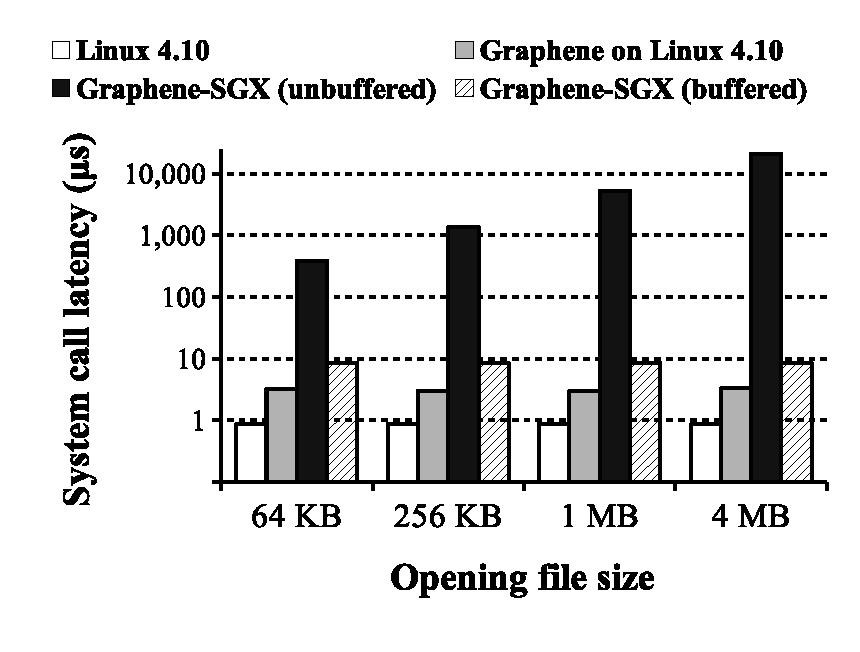
\includegraphics[width=\linewidth]{sgx/open-latency}\\
\vspace{3pt}
{\bf (a) Opening a file}
\vspace{6pt}
\end{minipage}
\begin{minipage}{.49\textwidth}
\centering
\footnotesize
\vspace{6pt}
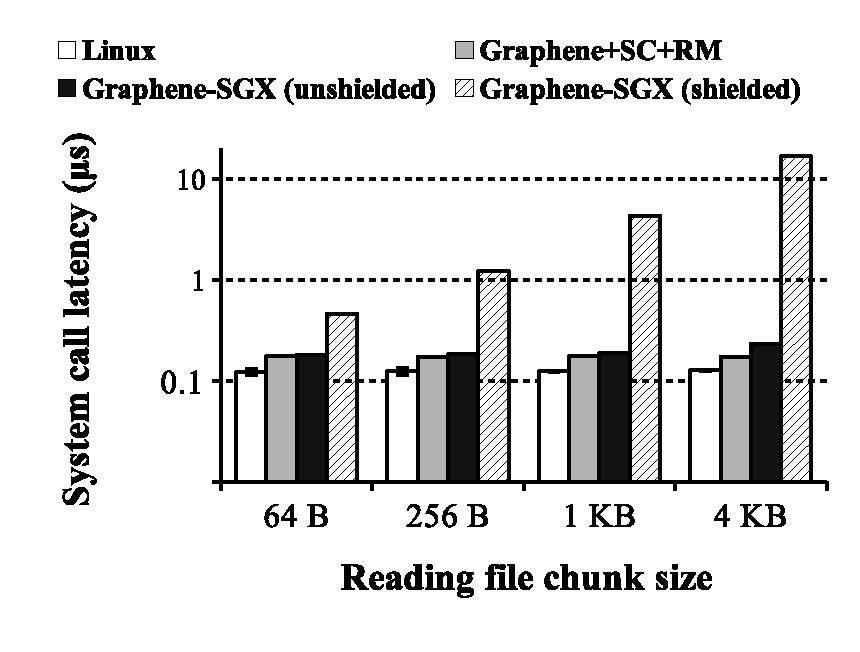
\includegraphics[width=\linewidth]{sgx/read-latency}\\
\vspace{3pt}
{\bf (b) Reading a file}
\vspace{6pt}
\end{minipage}
\caption{Latency of some expensive system calls in \graphenesgx{}, including opening and reading a secured (authenticated) file, and forking a new process. The results are compared with native Linux and \graphene{}.}
\label{fig:eval:sgx-shield-syscall}
\end{figure*}


Figure~\ref{fig:syscall}(a)
shows the overhead for authenticating files in \syscall{open}.
\fixme{change overhead to latency}
Depending on the file size, the latency of \syscall{open} on \graphenesgx{} is 383$\mu$s (64KB file) to 21ms (4MB file), whereas on Linux, the latency is constant at 0.85$\mu$s.
We note that this is where enclaves are at a disadvantage, as \syscall{open} 
normally does not need to read file content; whereas here \graphenesgx{} uses \syscall{open}
as a point at which to validate file content.
For a subsequent \syscall{open}, when the Merkle tree is already generated, the overhead of simply exiting enclave for \syscall{open}, and searching the file list in the manifest, is about 9$\times$.
%\fixmedp{why?}


One might be able to optimize further for cases where only part of a file is accessed
with incremental hashing.  However, in the common case where nearly all of the file is accessed,
these costs are difficult to avoid when host file system is untrusted.
Another opportunity 
is to create the Merkle tree offline, when the manifest is created.
%\fixmedp{I think the second idea has legs...}


%This is an inevitable cost, because normal \funcname{open} on trusted OSes
%need not to access file content.
%After verifying the file, \graphenesgx{} buffers the chunk hash values, to skip whole-file verification when the file is reopened.

Figure~\ref{fig:syscall}(b)
shows the overhead for authenticating files in \syscall{read}, which 
is lower than \syscall{open}.
Since the whole file has been verified at \syscall{open}, the sequential \syscall{read} only verifies the chunks of files it is reading from untrusted memory.
%Reads from data cached in enclave memory are cheaper.  %\fixmedp{right? can we say how much cheaper?  Maybe add separate bars for both cases?}
% Therefore, \syscall{read} is actually much cheaper than \syscall{open}.
Depending on the size of blocks being read, the latency on \graphenesgx{} is 0.5$\mu$s (64-byte \syscall{read}) to 16.9$\mu$s (4KB \syscall{read}). The latency of \syscall{read} on Linux is \roughly{}0.1$\mu$s for any block size below 4KB.
If the file is not authenticated,
\graphenesgx{} only copies the file contents into the buffer, and the overhead reduces to 48\% (64-byte \syscall{read}) to 83\% (4KB \syscall{read}).
\fixmedp{Consider doing larger buffers, say up to 64k or even 4 MB}

%\fixmedp{In the legend for 7b, unsecure should be insecure}


\subsubsection{\syscall{fork} and \syscall{execve}}


\begin{table}[t!b!]
\footnotesize
\centering
\begin{tabular}{|l|rr|rrr|rrr|}
\hline
{\bf Test } & \multicolumn{2}{c|}{{\bf Linux}} & \multicolumn{3}{c|}{{\bf \graphene{}
}} & \multicolumn{3}{c|}{{\bf \graphene{} + SC + RM}} \\
&
\usec{} & +/- & 
\usec{} & +/- & \%O &
\usec{} & +/- & \%O \\

\hline
fork+exit      &  66.86 & 0.09 &   380.47 & 3.55 & 469 &   442.83 & 1.39 &   562   \\\hline
fork+fork+exit & 148.32 & 0.55 &   778.00 & 6.87 & 424 &   915.67 & 3.35 &   517   \\\hline
vfork+exec     & 141.53 & 0.18 &   487.67 & 5.05 & 245 &   547.30 & 5.22 &   286   \\\hline
fork+exec      & 194.93 & 0.20 &   810.00 & 3.27 & 315 &   878.50 & 1.89 &   350   \\\hline
fork+fork+exec & 266.89 & 0.36 & 1,200.60 & 5.20 & 349 & 1,387.75 & 6.21 &   420   \\\hline
fork+sh        & 499.64 & 0.67 & 1,726.75 & 6.14 & 245 & 1,912.00 & 3.83 &   283   \\\hline
%\hline
%UDP lat.&7.26&0.0&10.35&0.1&43&11.63&0.1&60 \\\hline
%TCP lat.&8.70&0.0&9.84&0.1&13&11.48&0.1&32 \\\hline
%\hline
%%%  \bf{Test} & K/s & +/- & K/s & +/- & \%O & K/s & +/- & \%O \\\hline
%%% %% \bf{Test} & \bf{K/s} & \bf{+/-} & \bf{K/s} & \bf{+/-} & \bf{\%O} & \bf{K/s} & \bf{+/-} & \bf{\%O} \\\hline
%%% 0K creat & 174 & 0.9 & 72 & 0.1 & 143 & 77 & 0.2 & 125 \\\hline
%%% 0K del & 232 & 1.2 & 130 & 0.5 & 79 & 117 & 0.2 & 98 \\\hline
%%% 4K creat & 120 & 0.1  & 33 & 0.0 & 265 & 31 & 0.0 & 284 \\\hline
%%% 4K del & 184 & 1.3  & 112 & 0.1 & 64 & 104 & 0.2 & 78 \\\hline
%%% 10K creat & 83 & 0.1  & 28 & 0.0 & 195 & 27 & 0.0 & 204 \\\hline
%%% 10K del & 149 & 0.3  & 94 & 0.1 & 58 & 88 & 0.2 & 69 \\\hline
\end{tabular}
\caption[\lmbench{} benchmarking results in Linux, KVM and \graphene{}]
{\lmbench{} comparison among (1) native Linux processes, (2) \graphene{} \picoprocs{} on Linux host, both without and with the SECCOMP filter ({\bf +SC}) and reference monitor ({\bf +RM}), and (3) \graphene{} in SGX enclaves.
Execution time is in microseconds, and lower is better. 
%The file system is measured in thousands operations per second, and higher is better.
Overheads are relative to Linux; negative overheads indicate improved performance.} 
\label{tab:graphene:lmbench}
\end{table}



Figure~\ref{fig:syscall}(c) shows the overhead of forking a process.
As described in \ref{sec:sgx:shield-multiproc}, the latency of \syscall{fork} in \graphenesgx{} is affected by three factors:
creation of a new enclave, local attestation of the integrity, and duplicating the process state over an encrypted RPC stream.
Combining these factors, \syscall{fork} is one of the most expensive calls in \graphenesgx{}.
%, but at least it is supported natively on the current hardware.
The default enclave size is 256MB.
%which takes \roughly{}0.5s to create. 
Our evaluation shows that the latency of forking a process is around 0.8s (16MB process) to 2.7s (128MB process), but can be more expensive if the parent process uses more memory.
The trend matches the performance of \graphene{} without the bulk IPC optimization.
\fixmedp{If you want, some thoughts on how this might be improved in the future would be nice...  One good suggestion is recycling enclaves, or pre-forking so measurements can be done in parallel}
%Due to the overhead on \funcname{fork}, \graphenesgx{} is not suitable for fork-intensive workloads like Bash scripts
%if performance is critical.

\fixme{talk about a limitation of improving fork. check this.}
One way to further optimize \syscall{fork} is to reduce or avoid enclave creation time; one can potentially pre-launch a child enclave, and then migrate the process contents later when \syscall{fork} is called.
There might be another opportunity to improve the latency of process migration,
if copy-on-write sharing of enclave pages can be supported in future generations of SGX.
%Unfortunately, sending the process contents is difficult to avoid in \syscall{fork},
%as SGX disallows sharing enclave memory between multiple enclaves.

%\fixmedp{I assume 5.4 isn't done yet}


%Adding more detail of KVM environment
%Unless otherwise noted, \graphenesgx{} measurements include the Phosphor instrumentation.





\begin{figure*}[t!]
\centering
\begin{minipage}{.45\textwidth}
\centering
\footnotesize
\vspace{6pt}
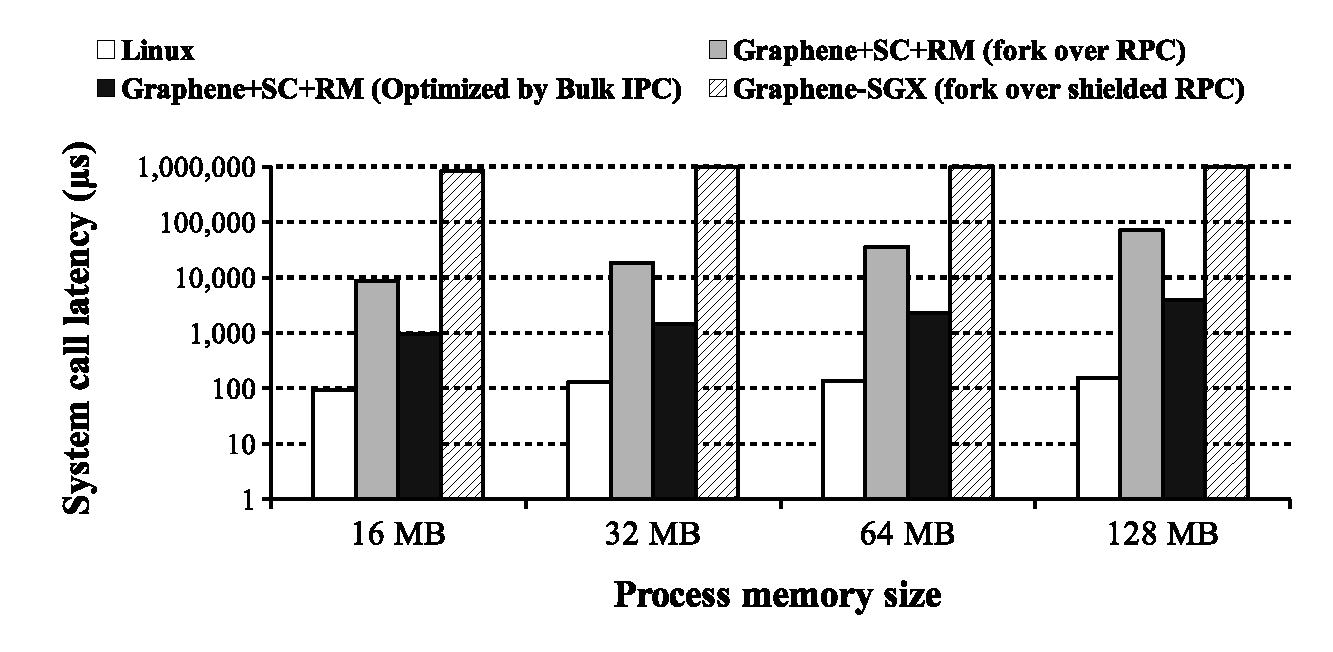
\includegraphics[width=\linewidth]{sgx/fork-latency}\\
\vspace{3pt}
{\bf (c) Fork a process}
\vspace{6pt}
\end{minipage}
\caption{Latency of some expensive system calls in \graphenesgx{}, including opening and reading a secured (authenticated) file, and forking a new process. The results are compared with native Linux and \graphene{}.}
\label{fig:sgx-shield-fork}
\end{figure*}


%\section{User-level {\tt fork} and other Linux library OS challenges}
%%% \vspace{5pt}
%%% \label{sec:fork}
%%% \noindent {\bf Copy-On-Write Fork.~}
%%% Creating a clean guest eases reasoning about security isolation, as all shared abstractions
%%% must be implemented using explicit data streams  between guests.
%%% This section describes how we implement these Unix abstractions in the guest
%%% %achieve a sensible division of labor between guest and host, and 
%%% without baking Unix personality into the host ABI.


\begin{comment}
\vspace{5pt}
\noindent{\bf Guest self-migration.~}  One of the key features of the host ABI
is that guest state can be programmatically read and recreated.
As a result, guests can checkpoint, migrate, and resume themselves in a new picoprocess,
potentially on a new host.  
Most of the library OS and application state are checkpointed simply 
by copying the contents of virtual memory into a file.
Checkpointing requires manually serializing a few key data structures
in {\tt libLinux} that are needed to resume the library OS from a checkpoint,
% interface directly with the PAL, 
including the thread states, handle table, and memory mappings.  

Resuming from a checkpoint involves restoring these key data
structures (handles, thread register contexts, memory mappings), and re-loading memory
contents from the checkpoint.  Most additional data structures
in {\tt libLinux}, and all application data structures,
are reloaded at the virtual address as before the checkpoint and work without modification.
\end{comment}

\begin{comment}
When a new guest begins execution, an input argument to {\tt libLinux} indicates
whether control should be transferred to the Linux loader ({\tt ld.so}) to start a new application instance, 
or whether a checkpoint should be loaded instead.
\end{comment}
%After the checkpoint is loaded, all threads resume execution on their stacks.


\section{Multi-process applications} 

%A characteristic of Linux application development is the opportunity of using one of 
This section explains an efficiency implementation of the process creation mechanisms in \thelibos{},
including \syscall{fork} and \syscall{execve}.
%and a variety of IPC (inter-process communication) mechanisms. 




\subsection{Forking a process}



Implementing the UNIX-style, copy-on-write forking presents a particular challenge to the \graphene{} architecture.
%when implemented using only a VM-like picoprocess abstraction.
Using \palcall{ProcessCreate} in \thehostabi{}, each \graphene{} host
creates a new \picoproc{} in a ``clean'' state, with an individual \thelibos{} instance maintaining the OS resources and features for an application process. % fork is implemented in the \libos{}.
%yet applications require common Unix abstractions such as file handle inheritance and copy-on-write fork.
Forking a process involves cloning the state of running application and migrating all the resource handles inside \thelibos{}, such as file descriptors, to the new \picoproc{}.
\graphene{} drops the assumption that each of its hosts is capable of sharing physical pages between multiple applications or processes.
Since \thelibos{} cannot enable copy-on-write sharing between \picoprocs{}, \thelibos{} needs an elaborate but efficient scheme for emulating the UNIX-style forking.


\issuedone{1.3.b}{describe the work flow of forking}
Without host support of copy-on-write sharing,
\thelibos{} emulates \syscall{fork} by checkpointing and migrating the process states.
When an application forks a process,
the current \thelibos{} instance holds a list of process resources that must be cloned for the new process.
By checkpointing the process states,
\thelibos{} creates a snapshot of the current process,
which is expected to the initial state
of the new process,
%expects to be reproduced to new process,
except a few minor changes.
A process snapshot includes all allocated resources, such as VMA and file handles,
and miscellaneous process states, such as signal handlers.
After checkpointing,
\thelibos{} calls \palcall{ProcessCreate} to create a new \picoproc{} in the host, and then migrates the process snapshot over the process handle as a RPC stream. %so that the state of the forking process is faithfully migrated to a new \thelibos{} instance.


To fully emulate \syscall{fork}, \thelibos{} implements
a checkpoint and migration scheme
for duplicating the resource handles and application states between \picoprocs{}.
For each type of resources, \thelibos{} defines a function for decomposing a resource handle in a migratable form,
and a function for reconstructing the resource handle inside another \picoproc{}.
For example,
for a VMA handle, \thelibos{} checkpoints the address, size, initial flags, and page protection,
and only if the VMA is accessed by the application and not backed by a file,
\thelibos{} copies the memory data into the snapshot.
For a file or network handle,
\thelibos{} runs a virtual file system operation,
\funcname{vfs\_checkout},
to externalize the related states
inside the file system implementations,
but skip any temporary states such as buffers and directory cache entries.
Finally, \thelibos{} checkpoints the current thread handle, but modifies the handle snapshot with a new process ID.



The checkpoint and migration scheme of \thelibos{} is comparable to
VM migration by a hypervisor.
When migrating a VM, a hypervisor has to copy the VM's guest physical memory to another host machine.
A useful feature of a hypervisor is to migrate a live VM,
and to implement the feature, the hypervisor needs hardware support for marking the dirty pages when it is copying the pages.
\graphene{} also implements live migration of a \picoproc{} for \syscall{fork}
because of the general expectation
that \syscall{fork} should not halt the whole process.
However, unlike live VM migration, \graphene{} chooses not %adopt the technique of live VM migration
copy the whole virtual address space
of a \picoproc{}
%Instead, the checkpoint scheme of \thelibos{}
%locks each handle when copying it to the heap or over a RPC stream
%\graphene{} chooses not to copy the whole virtual address space 
for three primary reasons.
First, a checkpoint scheme that snapshots the whole \picoproc{}
cannot differentiate temporary and permanent states inside a \libos{}.
To improve I/O performance, \thelibos{} tends to reserve %a significant amount of
virtual memory for caching and buffering, and \thelibos{} can reduce migration time by skipping temporary states such as directory cache entries and I/O buffers.
Second, by checkpointing handles individually,
\thelibos{} can overwrite each handle and sanitize any sensitive states before sending the snapshot out to another \picoproc{}.
Finally, \thehostabi{} does not export any functionality for tracing
the dirty pages during live migration,
because the low-level hardware support needed
is not available on a more restricted hardware like Intel SGX.
For all the reasons above,
\thelibos{} only selectively checkpoints \libos{} states rather than snapshotting the whole \picoproc{}.


%new \picoproc{} cannot reuse PAL handles snapshotted from the previous \picoproc{}.
%Therefore, after migrating the whole virtual address space,
%either \thelibos{} has to scan its internal heap to recreate or nullify all the PAL handles, or \thehostabi{} has to detect any migrated PAL handles.
%Moreover, to consistently snapshot a \picoproc{},
%\thelibos{} has to stop the execution of every running threads,
%or iteratively trace dirty pages after copying a certain amount of pages to the snapshot.
%Either approach requires more control over host-level page management
%in order to prevent significant interruption in the application.






%Rather than writing the checkpoint to a file, 
%we developed an efficient bulk IPC mechanism to 
%permit copy-on-write sharing of memory pages among processes.
%Bulk IPC is a performance optimization over sending each byte of the parent address
%space over a stream, although {\tt libLinux} can also implement {\tt fork}
%over a stream.
%Bulk IPC adds 3 calls to the host ABI,
%and the host reference monitor only permits bulk IPC among
%picoprocesses within a sandbox.

%% Conceptually, {\tt fork} could be implemented by checkpointing the parent,
%% modifying the primary thread's checkpoint 
%% so that the child returns 0 from the fork call 
%% (indicating it is the child),
%% and then immediately resuming the checkpoint in another picoprocess.

%% In practice, we optimize {\tt fork} performance by avoiding 
%% the use of an intermediate checkpoint file, instead transferring the checkpoint
%% directly to the child over a host-level bulk IPC
%%  mechanism (\S\ref{sec:linux:pal}).
%The Graphene bulk IPC abstraction adds 3 PAL calls 
%that allow guests to efficiently transfer large regions of memory to each other\fixmedp{after reordering, add a forward or back ref}.



Migrating process states over a RPC stream adds a significant overhead to the latency of \syscall{fork} in \thelibos{}.
To reduce the overhead, \graphene{} introduces a {\bf bulk IPC} mechanism in \thehostabi{}, to send large chunks of memory across \picoprocs{}. 
Using the bulk IPC mechanism, 
%Using our bulk IPC mechanism,
the sender (i.e., the parent) can request the host kernel
to preserve the physical pages of application memory and snapshot data,
and the receiver (i.e., the child) can map these physical pages to its own virtual address space.
This bulk IPC mechanism is an efficiency way of sending pages out-of-band,
while the parent process still uses a RPC stream
to send control messages including the parameters of bulk IPC.
Although the implementation is up to the host kernel,
the bulk IPC mechanism should map the same physical pages in both parent and child,
to minimize the memory copy in the host kernel.
The host kernel marks the physical pages copy-on-write in both \picoprocs{},
to ensure that the child receives a snapshot of the sent pages from the parent without sharing any future changes.
The bulk IPC mechanism is optional in \thehostabi{},
and \thelibos{} can always fall back to sending process snapshots over RPC streams
when the host fails to support bulk IPC.



%Our IPC module is \gipclines{} lines of code (Table~\ref{tab:graphene:loc}), 
%runs on multiple versions of Linux (2.6 and 3 series kernels), and
%does not require
%Linux kernel changes or recompilation.


\begin{comment}
A critical challenge in developing a Linux library OS was implementing 
handle inheritance in the guest.  In some cases, 
handles are easy to reproduce: an open file can simply be reopened in the child,
and the cursor offset adjusted (note that file handle offsets are a library abstraction
implemented over a memory mapped file).
Pipes, however, are not easily recreated without host support.
\end{comment}
%One option was to create explicitly named host-level byte streams,
%similar to System V or Windows named pipes.
%This strategy is simple to add to the Drawbridge host ABI and easy to program in {\tt libLinux},
%but complicates security isolation, as guests must be prevented from 
%opening a host-level pipe outside of their sandbox.

%A second option, which we pursue, is to only create anonymous bytes streams,
\paragraph{Inheriting PAL handles.}
When a file handle to the child, \thelibos{} sometimes needs to send the stored PAL handle, especially when the file handle
represents a network socket or a deleted file.
\thelibos{} normally nullifies the PAL handle in the snapshot of a file handle
since the PAL handle is only valid for the local PAL.
However, if \thelibos{} cannot recreate a PAL handle by calling \palcall{StreamOpen} in the child \picoproc{}, \thelibos{} needs host support to inherit
the PAL handle from the parent.
There are generally two conditions when the child process
cannot recreate a PAL handle.
First, a \picoproc{} cannot reopen a bounded network handle
if another \picoproc{} still holds the local port.
Second, the parent process may delete a file while holding a file descriptor to access the file content, generally as a way of detaching the file from the file system.
If the file is deleted in the host file system,
the child process cannot reopen the file
using \palcall{StreamOpen}.



\thelibos{} uses two new \hostapis{},
\palcall{RPCSendHandle} and \palcall{RPCRecvHandle}, to send PAL handles out-of-band over a PRC stream.
As \thelibos{} walks through a file handle list for checkpointing, it marks the PAL handles that are network sockets or deleted files.
If the parent deletes a file after migrating the file handle but before the child recreates the PAL handle,
the child will either fail to reopen the file
or accidentally open another file created afterward.
\thelibos{} can detect this corner case by coordinating the file system states
across \picoprocs{}.



% within a sandbox.  Handle passing facilitates inheritance
%and general-purpose RPC.
%This mechanism is similar to Unix Domain Sockets,
%which are commonly used by sandboxing systems. % such as plash~\citep{plash}.
%This strategy allows a guest to seamlessly and explicitly 
%share an open handle with another guest in the same sandbox, but prevents
%a guest from sharing a handle with a guest outside of the sandbox.

\begin{comment}
\vspace{5pt}
\noindent{\bf Discussion.~}
A Graphene picoprocess can copy part or all its address space into a child
picoprocess relatively efficiently.
Although this mechanism is less efficient than an in-kernel {\tt fork},
we wanted to maintain the generality benefits of recent \liboses{},
and only added the minimal building blocks to the host ABI.
%we felt this design would bake Unix personality into the host kernel ABI,
%and  reintroduce security problems caused by accidental inheritance~\citep{close-on-exec}.
The transfer of data is explicit to the host, can be mediated by a reference monitor,
the sender, or the receiver.
For instance, recent Unix systems introduced a close-on-exec flag for file handles~\citep{close-on-exec}, 
which prevents inheritance of handles to sensitive files.  This can be implemented
either in a parent, by excluding the file handle from a checkpoint, 
or in the child, by closing this handle on an {\tt exec} call.
Our current implementation implements close-on-exec in the child for complete compatibility,
but a more security-sensitive application could easily implement ``close-on-fork'' semantics 
in the parent.
This clean division of labor retains full functionality
and facilitates extensibility.


\end{comment}

%\issue{1.3.b}{discuss alternative strategies of forking}


\subsection{Process creation with \syscall{execve}}


Another Linux \linuxapi{}, \syscall{execve}, creates a process with a separate executable and a clean memory state.
The specification of \syscall{execve}
includes detaching the calling thread from a process and moving it to a brand-new virtual address space with the specified executable.
As a common use case, a shell program (e.g., Bash) calls \syscall{execve} after creating a thread using \syscall{vfork},
to execute a shell command (e.g., \code{ls}) in a separate process, while the main process continues and waits for the shell command to finish.
%When one thread in a multi-threaded process
%calls \syscall{execve}, other running threads still run in the same context.
%Instead, \syscall{execve} creates a process
%with the same credentials of the calling thread, but the process runs a fresh, separate executable from the parent.
%Calling \syscall{execve} from a multi-threaded process 
%is especially common in a shell program (e.g., Bash).
%A shell program often calls \syscall{execve} after \syscall{vfork} to execute a command in a new process monitored by the job controller, similar to \funcname{spawn} in the POSIX API.
Linux uses the combination of \syscall{vfork} and \syscall{execve}
as an equivalent of \funcname{spawn} in the POSIX API, or \funcname{CreateProcess} in the Windows API.


\thelibos{} implements \syscall{execve} by calling \palcall{ProcessCreate} with
the host URI of the executable,
and selectively migrating process states to the new \picoproc{}.
When the application calls \syscall{execve} to run an executable, \thelibos{} first has to identify the executable on the chroot file systems,
to determine its host URI for creating a \picoproc{}.
Although \palcall{ProcessCreate} achieves the goal of creating a clean process with the target executable,
\syscall{execve} further specifies that the child must inherit the parent's credentials and file descriptors, except file descriptors opened with a \code{CLOEXEC} flag.
\thelibos{} uses the same checkpoint and migration scheme in \syscall{fork} to selectively migrate handles and \libos{} states in \syscall{execve}.
The states migrated in \syscall{execve}
include the caller's thread handle, all the non-\code{CLOEXEC} file handles, program arguments and environment variables given by the application, and global OS states that are shared across \thelibos{} instances
(e.g., namespace information).




\papersection{Coordinating guest OS states}
\label{sec:libos:namespaces}

%\fixmedp{RF: what are the few, powerful mechanisms?  Expect that there are many cases 
%with shared state; re-read this to see if it is clear how to generalize the approach}

%Recent library OS designs focus on single-process applications,
%which move a substantial portion of the OS APIs and state used by the application into the \libos{}.

%A key contribution of the \graphene{} 
%design is robust and flexible support for multi-process applications.
A multi-process application executes on \graphene{} 
with the abstraction that all of its processes runs on a single OS.
Each \thelibos{} instance services system calls
from its local state whenever possible.
However, whenever a \thelibos{} instance must share a \libos{} state with other instances,
\thelibos{} has to coordinate the state across \picoprocs{}
via an RPC stream.
Within a sandbox, multiple \picoprocs{} 
can securely coordinate shared states of multi-process abstractions, including process IDs, exit notification and signaling, 
System V IPC mechanisms (message queues and semaphores), shared file system states, and shared file descriptor states (Table~\ref{tab:libos:multiproc}).
%Similar to previous \liboses{}~\cite{porter11drawbridge,baumann13bascule}, 
%\graphene{} uses the host file system; 
%the \libos{} implements file handles and translates between POSIX and the host ABI.
%Identifying the best division of labor for a \libos{} file system is 
%left for future work.
\thelibos{} contains a coordination framework
with several building blocks for implementing a shared multi-process abstraction.

\begin{table}
\footnotesize
\centering
\begin{tabular}{|p{.16\textwidth}|p{.20\textwidth}|p{.55\textwidth}|}
\hline
{\bf Ab\-strac\-tion} & {\bf Shared State} & {\bf Coordination Strategy} \\
\hline
Fork & 
\raggedright
PID namespace & Batch allocations of PIDs, children generally created using local state at parent.  \\
\hline
Signaling & PID mapping & Local signals call handler; remote signal delivery by RPC.  Cache mapping of PID to \picoproc{} ID. \\
\hline
\raggedright
Exit notification & 
\raggedright
Process status  & Exiting processes issue an RPC, or one synthesized if child becomes unavailable.  The {\tt wait} system call blocks until notification received by IPC helper. \\
\hline
{\tt /proc/[pid]} & Process metadata & Read over RPC.  \\
\hline
Message Queues & 
\raggedright
Key mapping \newline
Queued messages &
Mappings managed by a leader, contents stored in various \picoprocs{}.  When possible, send messages asynchronously, and migrate queues to the consumer.\\
\hline
Semaphores & 
\raggedright
Key mapping \newline
Semaphore count &
Mappings managed by leader, migrate ownership to \picoproc{} most frequently acquiring the semaphore. \\
\hline
\raggedright
File System & 
\raggedright
File truncate sizes \newline
Deleted files \newline
FIFO \& domain sockets
& No coordination; completely relying on \thehostabi{}; creating special files in the host to represent symbolic links. \\
\hline
\raggedright
Shared File Descriptors & 
\raggedright
Seek pointers & Mappings managed by parent, migrate ownership to \picoproc{} most frequently accessing the file descriptors. \\
\hline
\end{tabular}
\caption{Multi-process abstractions implemented in \graphene{}, coordinated state, and implementation strategies.}
\label{tab:libos:multiproc}
\end{table}


%% Outline

% Basic idea of what we are doing
% Building blocks
% Implemented abstractions and examples (table)
%% Why not shared FDs?
% Optimizations/insights
% Why different from microkernels?



As an example of balancing security isolation and coordination APIs,
consider functionality that accesses the process ID namespace,
such as UNIX signaling or exit notification (e.g., {\tt waitpid()}).
In \graphene{}, the process ID namespace, 
as well as signaling and related system calls,
are implemented inside \thelibos{}.
A process can signal itself by having the \libos{} directly call the handler function.
When \picoprocs{} are in the same sandbox, they coordinate
to implement a consistent, shared process ID namespace,
as well as to send and receive signals amongst themselves.
\thelibos{} implements inter-process signaling using RPC messaging.
When \picoprocs{} are in separate sandboxes,
they do not share a PID namespace, and cannot send signals to each other.
The reference monitor ensures that IPC abstractions, such as signaling,
cannot escape a sandbox by preventing the creation of kernel-level streams
across sandboxes.



%Figure~\ref{fig:libos:sandbox} illustrates several sandboxes with \picoprocs{}
%collaborating to implement a process ID namespace.  
%Because this namespace is a guest-level abstraction,
%different sandboxes can have overlapping process IDs, and
%cannot signal each other.
%If the connection between the two \picoprocs{} on the right of the figure
%is severed by subdividing the sandbox,
%the processes will become inaccessible to each other
%and each newly isolated library OS will treat the event as a process termination.
%%\fixmedp{See if we can get a better figure}

%dp:  Seems redundant, probably imported from S2
\begin{comment}
Within a sandbox, each library OS tracks the PIDs of other \picoprocs{}.
As children are created, each library OS updates its own replica of the 
process tree, with annotations for which host-level connection corresponds
to the remote process.  
If a \picoproc{} signals itself, the signal system call simply calls the 
appropriate signal handling function in the application. 
If a \picoproc{} signals another \picoproc{},
the signal essentially becomes an asynchronous remote procedure call
from the sending library OS to the receiving library OS.
Note that this is all transparent to the unmodified application.
Section~\ref{sec:graphene:namespaces} describes these library OS-internal
coordination mechanisms in more detail.
The current \graphene{} prototype supports 
a range of coordination abstractions, including signaling, 
exit notification, System V message queues, thread identifiers and groups, sessions,
and the process tree.
We believe this sample is sufficiently representative that
remaining tail of Linux IPC abstractions could be easily added.

The reference monitor ensures security isolation
simply by preventing \picoprocs{} in different sandboxes from 
sharing host-level streams.
We adopted this approach to maximize dynamic sandboxing flexibility,
rather than, say, attempt to multiplex one single library OS instance across multiple processes.
\end{comment}


A driving design insight is that the common case
for coordination is among pairs of processes.
Examples include a parent waiting for a child to exit, 
one process signaling another, or a single producer and single consumer
sharing a message queue.
Thus, \graphene{} optimizes for the common case of pairwise coordination,
reducing the overhead of replicating data (see Section~\ref{sec:libos:namespaces:lessons}).


%The rest of this section describes our coordination framework, 
%beginning with the coordination building blocks,
%and then explains the implementation of several multi-process abstractions.
%We conclude with lessons learned from optimizing  multi-process performance.

Although a straightforward implementation worked, tuning the performance was the most challenging aspect of the coordination framework. 
This section summarizes the lessons learned during the development of \graphene{}, from optimizing the coordination of various multi-process abstractions.
This section then
presents the design and driving insights of the coordination framework,
followed by representative examples 
and a discussion of failure recovery.

\papersubsection{Building blocks}
\label{sec:libos:namespaces:building-blocks}

The general problem underlying each of the coordinated \libos{} states is 
the coordination of {\bf namespaces}.  In other words, coordination between processes needs 
a consistent mapping of names, such as process IDs or System V IPC resource keys, 
to the \picoproc{} implementing that particular item.  
Because many multi-process abstractions in Linux can also be used by single-process applications,
a key design goal is to seamlessly transition between single-process cases, serviced 
entirely from local \libos{} state, and multi-process cases, which coordinate shared abstractions over RPC.

%Picoprocesses then implement abstractions such as signals
%by issuing a remote procedure call (RPC) to the appropriate \picoproc{}.

\thelibos{} creates an {\bf IPC helper} thread within each \picoproc{}
to respond to coordination messages from other \picoprocs{}. 
%within the sandbox. %, using these broadcast and point-to-point streams.
An IPC helper
maintains a list of point-to-point RPC streams, and indefinitely waits for incoming messages.
For each multi-process abstractions coordinated over RPC,
\thelibos{} defines a protocol for formatting the header of each message
and determining the callback function for processing the message.
GNU Hurd~\cite{hurd} has a similar helper thread to implement signaling among a process's parent and
immediate children;
\graphene{} generalizes this design to share a broader range of multi-process abstractions among any \picoprocs{}.
An IPC helper serves remote messages and receive responses atomically,
and is created in each \picoproc{}
after the application spawned its first child process.
For avoiding deadlock among application threads and the IPC helper thread, 
an application thread may not both hold locks required by the helper thread to service an RPC request
and block on an RPC response from another \picoproc{}.
All RPC requests are handled from local state and do not issue recursive RPC messages.% \fixmedp{Check this}

Within a sandbox, all IPC helper threads exchange messages using a
combination of
a {\bf broadcast stream} for global coordination,
and {\bf point-to-point} RPC streams for pairwise interactions, 
minimizing overhead for unrelated operations.
A PAL creates the broadcast stream the process as part of initialization.
Unlike other byte-granularity streams, the broadcast stream sends data at the granularity of messages,
to simplify the handling of concurrent writes to the stream.
Point-to-point RPC streams include the streams between parent and child processes established during \palcall{ProcessCreate},
and RPC streams created through connecting to an RPC server
identified by its URI.
% simply byte streams between two \picoprocs{};
%two processes may establish a point-to-point stream by passing handles through 
%an intermediate stream or over the broadcast stream.
%The handle-passing ABI is discussed further in Section~\ref{sec:graphene:impl}.
Because of the security isolation in the host,
only processes in the same sandbox can connect to each other through RPC.
%The broadcast stream is primarily used for failure 
%recovery (\S\ref{sec:namespaces:failurerecovery}); 
%Mmost operations use point-to-point streams to minimize overheads.
If a process leaves a sandbox to create a new one,
its broadcast stream is shutdown and replaced
with a new one, connected only between a parent process and any children created in the
new sandbox.

Because message exchange over the broadcast stream does not scale well,
we reduce the use of the broadcast stream to the minimum.
One occasion of using the broadcast stream is
{\bf process ID allocation}.
Because each process needs an unique ID to be recognized as a source or a destination of RPC messages, \thelibos{} generates a random number as the ID of each process and confirms use the broadcast stream to confirm uniqueness.
Another occasion of using the broadcast stream
is {\bf leader recovery}, which happens when a namespace leader unexpectedly crashes
during coordination. For the implementation of leader recovery, see Section~\ref{sec:libos:namespaces:details}.


For each namespace (e.g., process IDs, System V IPC resource keys), \thelibos{} elects one of the processes in a sandbox to serves as the {\bf leader}.
A leader is responsible for
managing and memorizing the allocation of identifiers or resources in a namespace,
in behave of all other processes.
For a namespace like the process ID namespace,
the leader subdivides the namespace for each process to reduce the RPC cost of allocation.
For example, the leader might allocate 50 process IDs to a process which intends to clone a new thread or process.
The process who receives 50 process IDs becomes the {\bf owner},
and can further assign the process IDs
to children without involving the leader.
For a given identifier, the owner is the serialization point for all updates,
ensuring serializability and consistency for that resource.
%%% the leader's IPC helper has the added responsibility of coordinating 
%%% global state (name allocations).
%%% Our design minimizes the role of the leader, instead distributing responsibility 
%%% to specific \picoprocs{} when practical.  
%%% If the leader crashes, 
%%% a new leader can be elected. The detail of leadership recovery is discussed in
%%% Section~\ref{sec:namespaces:leader}. 
%More detailed discussion of the \graphene{}-internal
%RPC protocol is omitted for space;
%but it 
%consists of 30 message types which 
%encode both state replication and RPC 
%messages.

\papersubsection{Examples and discussion}
\label{sec:libos:namespaces:details}

%This subsection describes \libos{} coordination by example.
%\vspace{5pt}
\paragraph{Signals and exit notification.}
{\tt libLinux} implements signals
in various ways according to the causes of signals.
For signals triggered by hardware exceptions (e.g., \code{SIGSEGV}),
\thelibos{} uses the hardware exception upcalls
in \thehostabi{}.
If a signal is sent from one of the processes for IPC purposes (e.g., \code{SIGUSR1}),
\thelibos{} exchanges RPC messages between \picoprocs{} to deliver the signal to the destination \picoproc{}.
%mplemented using a combination of 
%{\tt sigaction} data structures %adapted from Linux
%to track signal masks and pending signals;
%\pal{}-provided hardware exception upcalls (e.g., for {\tt SIGSEGV});
%and  RPCs for cross-\picoproc{} signals (e.g., for  {\tt SIGUSR1}).
If a process signals itself, {\tt libLinux} interrupts the targeted threads inside the process
and uses internal data structures
to call the appropriate user signal handler.
%this section describes how this local model is extended with RPCs for remote PIDs.
%For cross-process signals, we use the namespace coordination mechanism.
\thelibos{} implements all three of Linux's signaling namespaces:
process, process group, and thread IDs.
If a signal is sent for a process or a process group,
every threads within the process or the process group receives a copy of the signal,
even if the threads belong to different \picoprocs{}.


Exit notification in Linux is based on the same mechanism as signaling.
When a process exits, normally a \code{SIGCHLD} signal
is delivered from the child process to its parent,
to unblock the parent who might be waiting for exit notification using \syscall{wait} or \syscall{waitpid}.
Exit notification is always coordinated over RPC streams
between parent and child \picoprocs{}.



\begin{figure}
\centering
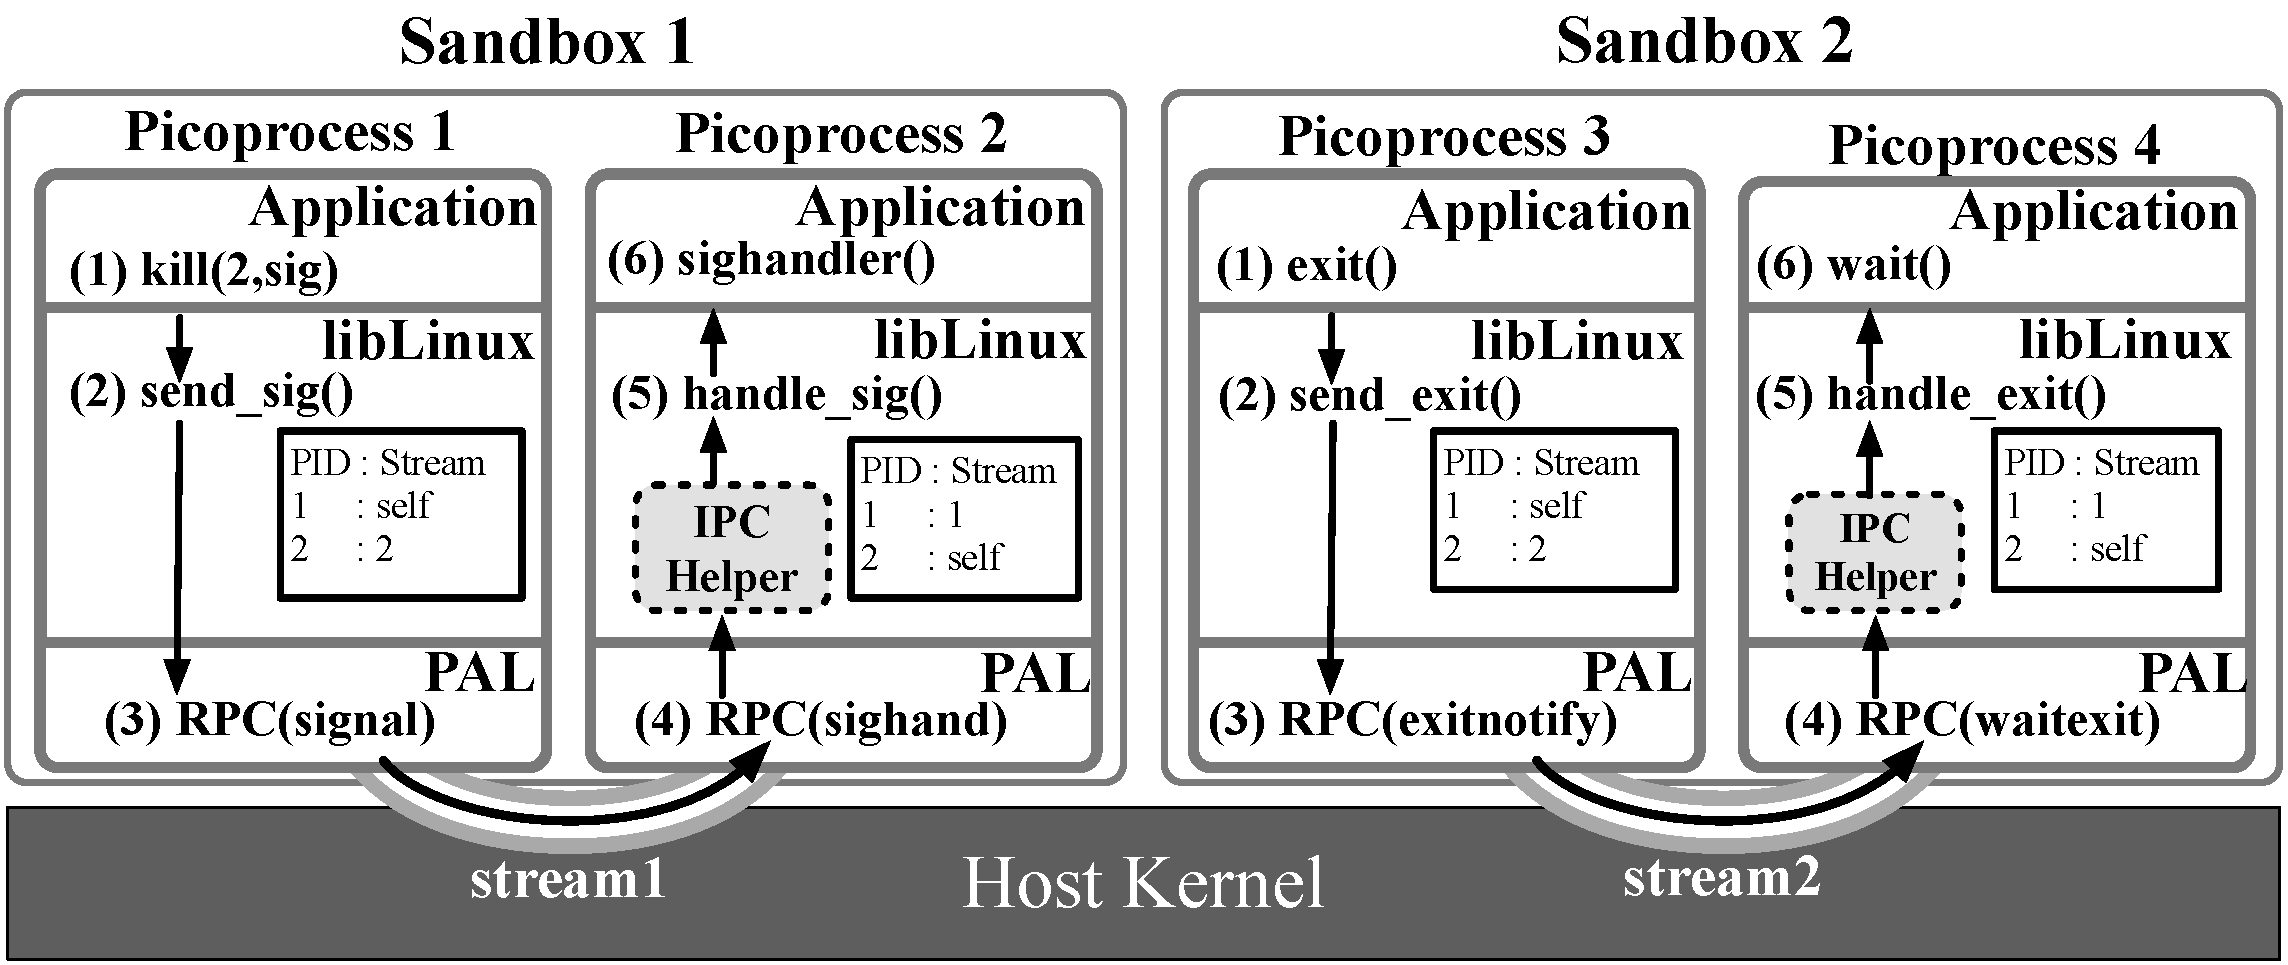
\includegraphics[width=36em]{coordination.pdf}
\caption{Two pairs of \graphene{} \picoprocs{} in different sandboxes 
coordinate signaling and process ID management.
The location of each PID is tracked in \thelibos{}; Picoprocess 1 signals
\picoproc{} 2 by sending a signal RPC over stream 1,
and the signal is ultimately delivered using a 
library implementation of the {\tt sigaction} interface. Picoprocess 4 
waits on an {\tt exitnotify} RPC from  \picoproc{} 3 over stream 2. }
\label{fig:libos:coordination}
\end{figure}


Figure~\ref{fig:libos:coordination} illustrates two sandboxes with \picoprocs{}
collaborating to implement 
signaling and exit notification
within their own
process ID (PID) namespaces.  
Because process IDs and signals are \libos{} abstractions,
\picoprocs{} in 
each sandbox can have overlapping process IDs, and
cannot signal each other.
The host reference monitor ensures that
picoprocesses in different sandboxes cannot 
exchange RPC messages or otherwise communicate.
%If the connection between \picoprocs{} 1 and 2 is severed by subdividing the sandbox,
%the processes will become inaccessible to each other
%and each newly isolated library OS will treat the event as a process termination.



If \picoproc{} 1 (PID 1) sends a \code{SIGUSR1} to \picoproc{} 2 (PID 2), illustrated in Figure~\ref{fig:libos:coordination},
a \syscall{kill} call to \thelibos{} will check its cached mapping of PIDs to 
point-to-point streams.
If \thelibos{} cannot find a mapping, it may begin by sending a query to the leader
to find the owner of PID 2,
and then establish a coordination stream to \picoproc{} 2.
%The leader may also pass a point-to-point coordination stream handle.
Once this stream is established, \picoproc{} 1 can send a  
signal RPC to \picoproc{} 2 (PID 2).
When \picoproc{} 2 receives this RPC, 
\thelibos{} will then query its local \code{sigaction} 
structure and mark \code{SIGUSR1} as pending.
The next time \picoproc{} 2 calls \syscall{kill},
the \code{SIGUSR1} handler will be called upon return. Also in Figure~\ref{fig:libos:coordination}, \picoproc{} 4 (PID 2) waits on 
\picoproc{} 3 termination (in the same sandbox with PID 1). When \picoproc{} 3 terminates, it invokes the library implementation of exit, which issues
an \code{exitnotify} RPC to \picoproc{} 4.
%In this example, \picoprocs{} in different sandboxes have the same PID number, but this does not cause conflict as they are isolated and can only communicate with processes in the same sandbox.

%%% Using a helper thread alongside each process to asynchro-
%%% nously handle signaling
%%% is common in many \microkernel{}-based OSes such as GNU Hurd~\cite{hurd}.
%%% GNU Hurd also maintains local mappings of PIDs and RPC ports for inter-process messaging.
%%% However, PID namespace in GNU Hurd is only tracked between the parents/children, so signaling cannot be transferred between arbitrary processes.
%%% \graphene{} handles PID namespace with global consistency inside a sandbox,
%%% but requires no intensive RPCs to any centralized service.   

The signaling semantics of \thelibos{} closely match the Linux behavior, which
delivers signals upon returning from a system call
or an exception handler.
Each process and thread have \code{sigaction} structures from the Linux source 
that implement the
POSIX specification, including handler functions, as well as masking signals and
reentrant behavior.
\thelibos{} does not modify \libc{}'s signal handling code. % is unmodified on \graphene{}.
%We extend the \pal{} with ABIs for explicit upcalls on certain hardware exceptions, such
%as divide-by-zero or segmentation faults.
%Signals from other processes, such as {\tt SIGUSR1}, are generally delivered upon 
%return from a call into {\tt libLinux}; 
If an application has a signal pending for too long,
e.g., the application is in a CPU-intensive loop, {\tt libLinux} can use \palcall{ThreadInterrupt} to interrupt the thread. 


% Daniela Oliveira commented. old caption for coordination
%\caption{\graphene{} namespace coordination example.  
 % Two applications and {\tt libLinux} instances
 % coordinate signaling and process ID management.
 % The location of each PID is tracked in {\tt libLinux};
 % a signal message is sent over a host stream
 % using the {\tt action} message, 
 % and the signal is ultimately delivered using a 
 % library implementation of the {\tt sigaction} interface.
%}


\begin{comment}
\graphene{} internally indexes point-to-point handles using PIDs.
In order to facilitate reallocation of PIDs without global coordination, 
\graphene{}-internal PIDs also include a {\em generation number},
allowing \picoprocs{} to lazily detect reuse similar to generation numbers 
for inodes in NFS~\cite{sandberg85nfs}.
\end{comment}

\paragraph{System V IPC.} System V IPC
maps an application-specified key onto a unique identifier.
All System V IPC abstractions, including message queues and semaphores,
are then referenced by a resource ID, which is arbitrarily allocated.
Similar to process IDs, 
%In order to service IPC requests, including identifier creation, from local state,
the leader divides the namespace of resource IDs among the processes,
so that any process
can allocate a resource ID from local state instead of involving the leader. %a pre-allocated range.
Unlike the resource IDs, System V IPC keys must be centrally managed
by the leader,
since an application might autonomously assign System V IPC keys to its processes.
%The leader also dynamically allocates keys to \picoprocs{}.
Global coordination is required to ensure that the same key maps to the same resource ID;
the leader caches this information, but the owner of the resource ID 
makes the definitive decision about whether a ID mapping is still valid.
A key which does not have a valid mapping can be assigned to a resource ID by any process to allocate a {\em private} IPC resource.



\paragraph{System V IPC message queues.} In \graphene{}, the owner of a queue ID is responsible for 
storing the messages written to a System V IPC message queue.
To ensure the serializability and consistency of all messages, any delivery and reception of messages must go through the owner.  
In the initial implementation of \thelibos{}, sending or receiving messages remotely over a RPC stream
orders of magnitude slower than accessing a local message queue.
This observation led to two essential optimizations.  
First, sending to a remote
message queue was made asynchronous.  In the common case, the sender can simply assume 
the send succeeded, as the existence and location of the queue have already been determined.
The only risk of failure arises when another process deletes the queue.
When a queue is deleted, the owner sends a deletion notification to all other \picoprocs{}
that previously accessed the queue.
If a pending message was sent concurrently with the deletion notification 
(i.e., there is an application-level race condition), 
the message is treated as if it were sent after the deletion and thus dropped.
The second optimization migrates queue ownership from the producer to the consumer,
which must read queue contents synchronously.

%\fixmedp{bill: it is referenced in the Semaphores section, but here there isn't any talk about migrating msg queues to the most active \picoproc{}. also, the section starts with ``two essential optimizations. First \ldots'', but there isn't a second. is queue ownership migration the second?}

Because non-concurrent processes can share a message queue,
our implementation also uses a common file naming scheme to serialize message queues to disk.
If a \picoproc{} which owns a message queue exits, 
any pending messages are serialized to a file in the host,
and the receiving process may regain the ownership of the message queue later from the leader and recover the serialized messages.
%In order to prevent happens-before violations in case of failure, 
%message queues may be checkpointed more aggressively.


%\paragraph{Failure Recovery.}
%\label{sec:namespaces:failurerecovery}
%The \graphene{} coordination protocols are designed such that the leader does not store any unrecoverable information---the leader
%only caches the current name allocations.
%Because we assume that \picoprocs{} within a sandbox trust each other, 
%a new leader can simply broadcast a request to 
%recreate the current name allocations.  
%If the leader crashes, a simple leader election protocol is sufficient, e.g., picking the smallest live PID.

%\daniela{I wonder if the remainder of this section should be part of implementation details(section 5)}

\paragraph{System V IPC semaphores.} System V IPC semaphores 
follow a similar pattern to message queues.
Each semaphore is owned by a \picoproc{};
a semaphore can be directly accessed by its owner as a local state,
whereas other \picoprocs{} all have to access the semaphore through the owner over RPC.
Since a semaphore shares the same performance pattern as a message queue,
\thelibos{} applies the same optimization
of migrating the ownership of a semaphore
%, where ownership of a given semaphore is migrated
to the \picoproc{} that most frequently acquires the semaphore.
%If the owner of a semaphore exits, \graphene{} transfers ownership to the leader.  rather than serialize the semaphore to disk.
Another optimization of message queues, by making the updates asynchronous,
does not apply to semaphores,
because a participating \picoproc{} cannot proceed before successfully acquiring the semaphore. 
Most of the overhead in the Apache benchmark (see Section~\ref{sec:eval:apps}) is attributable to semaphore overheads.
%and, in ongoing work, we will likely optimize this by 
%either expanding the host ABI to share synchronization primitives within a sandbox,
%using shared memory to reduce semaphore latency.

\paragraph{Shared file descriptors.}
The seek pointer of each file descriptor is implemented as a \libos{} abstraction;
when reading or writing to a host file,
\thehostabi{} always obtains an absolute pointer from the beginning of the file.
Although most applications
do not share the seek pointer of an inherited file descriptor among processes,
the {\tt clone} system call
can can be called with the {\tt CLONE\_FILES} flag
and create a process
which shares the whole file descriptor table with its parent.
%The default Linux behavior is that children copy the open handles and file seek cursors,
%but subsequent cursor movements are not shared between parent and child.
%Shared file descriptor table can be requested by passing the {\tt CLONE\_FILES} flag to the {\tt clone} system call.
%Any new file descriptor opened in a shared table will be visible by every process cloned in this way, as well as subsequent cursor update.
%None of our target applications have required a shared seek cursor, and it is not currently implemented,
%but would be a straightforward extension to current RPC mechanisms.
%We expect that the current RPC mechanisms could easily be extended to synchronize a seek pointer among \picoprocs{}.
To share a file descriptor table among \picoprocs{},
one of \picoprocs{} (usually the oldest one)
must be the leader of the file descriptor table to manage all mappings
from file descriptors to the child \picoproc{} who owns the state of the file descriptors including the seek pointers.
Every updates to a seek pointer must goes through the owner of the file descriptor (not the leader).
The migration-based optimization for System V IPC message queues and semaphores is also effective for optimizing the performance of shared file descriptors. 

\paragraph{Shared file system states.}
A chroot file system in \thelibos{}
is restricted by \thehostabi{} to externalize any file system states.
Other shared file system states are implemented as \libos{} abstractions, and have to be coordinated among \picoprocs{}.
For example, a POSIX file system can contain special files such as a FIFO (first-in-first-out); a path bound to a UNIX domain socket;
a symbolic link; or a file system lock.
Implementation of these special files cannot
completely depend on \thehostabi{},
since \thehostabi{} only supports regular files and directories.

%Coordinating these states can be cause significant slowdown on regular file system operations, so we simply export the state in regular files on the host,
% and atomically update them by renaming.

A simple approach to coordinating file system states is to share a ``dummy'' host file.
For example,  \thelibos{} can store the target of a symbolic link
in a regular file on the chroot file system.
For a FIFO, a bounded UNIX domain socket, or a file system lock,
\thelibos{} can store a mapping to the corresponding RPC stream, or to the \picoproc{} which owns the abstraction.
By using the host file system as a less efficient but permanent coordination medium,
\thelibos{} can extend the coordination framework for sharing file system states.



\paragraph{Shared memory.} The \graphene{} architecture 
does not currently permit shared memory among \picoprocs{}.
This thesis expects that an extra \hostapi{} and the existing support for System V IPC coordination would be sufficient to implement this,
with the caveat that the host must be able to handle sandbox disconnection gracefully, perhaps converting the pages to copy-on-write.
Thus far \graphene{} have avoided the use of shared memory in \thelibos{},
both to maximize flexibility in placement of \picoprocs{}, potentially on an unconventional host (e.g., Intel \sgx{}) or different physical machines.
and to keep all coordination requests explicit.
Shared memory may be useful to reduce latency for RPC messaging across \picoprocs{} on the same host.


%in \graphene{} are implemented by a simple producer-consumer model.
%%% Without blocking, the latency of an inter-process semaphore operation equals to a round-trip of RPC messages.
%%% We observed that IPC semaphores can benefit from the same optimization
%%% used by message queues,
%%% based on asynchronous sending.
%%% However, when non-concurrent processes share a semaphore, it does not worth serializing the semaphore state to disk.
%%% When the owner of a semaphore exits,
%%% the semaphore state will be migrated to the leader,
%%% if it has a non-zero counter.
%%% IPC semaphores are intensively used in Apache web servers with a multi-process model. 

 


\paragraph{Failure and disconnection tolerance.}  
\thelibos{} must tolerate disconnection between collaborating \picoprocs{},
either because of crashes or blocked RPC streams.  In general, \thelibos{} makes 
these disconnections isomorphic to a reasonable application behavior,
although there may be some edge cases that cannot be made completely transparent to the application.

In the absence of crash recovery, placing shared state in a given \picoproc{} introduces the risk that an errant 
application will corrupt shared \libos{} state.  The \microkernel{} approach of 
moving all shared state into a separate server process is more resilient to this problem.
Anecdotally, \thelibos{}'s performance optimization of migrating ownership to the process that 
most heavily uses a given shared abstraction also improves the likelihood that only the corrupted
process will be affected.  
Making each \thelibos{} instance resilient to arbitrary memory corruption of any \picoproc{} is left for future work.


\paragraph{Leader recovery.}
\thelibos{} provides a leadership recovery mechanism when a leader failure is detected.
A non-leader \picoproc{} can detect the failure of a leader by either observing the shutdown of RPC streams or timing out on waiting for responses. 
Once the \picoproc{} detects leader failure, \thelibos{} sends out a message on the broadcast stream to volunteer for claiming the leadership.
After a few rounds of competition, the winning \picoproc{} becomes the new leader and recover the namespace state by reading a namespace snapshot stored before the crash of the former leader
or recollecting from other \picoprocs{} in the same sandbox.

%After a \picoproc{} being elected as the leader,
%the leader state,
%including all the allocated IDs and the RPC stream addresses,
%must be recovered. 
%Recollecting the leader state from all the \picoprocs{} is possible
%but can be inefficient,
%given the new leader may not have knowledge about every \picoproc{}.
%To simplify the implementation,
%we make the leaders of a namespace periodically serialize their states to disk for later recovery.

When a \picoproc{} is moved to a new sandbox, \thelibos{} will naturally detect the failure of leader because of blocked RPC. % streams are closed by the reference monitor.
The sandboxed \picoproc{} will be the only candidate for leadership because the host has replaced the broadcast stream;
as a result, the sandboxed \picoproc{} seamlessly transitions to new namespaces isolated from the previous sandbox.

%Once it starts the leadership recovery, it will automatically win because no other \picoproc{} is sharing the broadcast stream. The procedure can be skipped by informing the sandboxed \picoproc{} before detaching.

\papersubsection{Lessons learned}
\label{sec:libos:namespaces:lessons}

The current coordination design is the product of several iterations, which began 
with a fairly simple RPC-based implementation. %, and was then refined based on profiling.
This subsection summarizes the design principles that have emerged from this process.
%We present high-level facets of the design along with the insight
%behind the decision.  The next subsections synthesize these aspects 
%with specific examples of signaling and message queues.

\paragraph{Service requests from local state whenever possible.}
Sending RPC messages over Linux pipes is expensive;
this is unsurprising, given the long history of 
work on reducing IPC overhead in microkernels~\cite{liedtke93sosp,chen93memory}.  
We expect that \graphene{} performance could be improved on a 
\microkernel{} with
a more optimized IPC substrate, such as L4~\cite{liedtke95sosp,klein09sel4,elphinstone13microkernels};
we take a complementary approach of avoiding IPC if possible.
%but this is beyond the scope of our work, and we want \graphene{} to perform well on any 
%host OS.

An example of this principle is migrating message queues to the ``consumer'' when a 
clear producer/consumer pattern is detected, or migrating semaphores to the most frequent requester.
In these situations, synchronous RPC requests can be replaced with local function calls, improving
performance substantially.  For instance, migrating ownership of message queues 
reduced overhead for messaging by a factor of $10\times$.

\paragraph{Lazy discovery and caching improve performance.}  
No library OS keeps a complete replica of all distributed state,
avoiding substantial overheads to pass messages replicating irrelevant state.
Instead, \graphene{} incurs the overhead of discovering the owner of a name
on the first use, and amortizes this cost over subsequent uses.
Part of this overhead is potentially establishing a point-to-point stream,
which can then be cached for subsequent use.
For instance, the first time a process sends a signal, the helper thread 
must figure out whether the process id exists, to which process it maps,
and establish a point-to-point stream to the process.
If they exchange a second signal, the mapping is cached and reused, amortizing this 
setup cost.  For instance, the first signal a process sends to a new processes
takes \roughly{}2ms, but subsequent signals take only \roughly{}55 \us{}.

\paragraph{Batched allocation of names minimizes leader workload.}
To keep the leader off of the critical path of operations like {\tt fork}, 
the leader typically allocates larger blocks of names, such as process IDs or System V queue IDs.
In the case of \syscall{fork}, if a \picoproc{} creates a child, it will request a batch of 
PIDs from the leader.  Subsequent child PID allocations will be made from the same 
batch without consulting the leader.
Collaborating processes also cache the owner of a range of PIDs, avoiding 
leader queries for adjacent queries.

%% dp: Sad to see this go, but it is sort of subsumed by the other discussion
\paragraph{Prioritize pairwise coordination within a sandbox.}
\graphene{} optimizes the common case of pairwise coordination,
by authorizing one side of the coordination to dictate the abstraction state,
but also allows
more than two processes to share an abstraction.
Based on this insight, 
we observe that {\em not all shared state need be replicated by all \picoprocs{}}.
Instead, we adopt a design where one \picoproc{} is authoritative for a given name (e.g., a process ID or a System V queue ID).
For instance, all possible thread IDs are divided among the collaborating \picoprocs{},
and the authoritative \picoproc{} either responds to RPC requests for this thread ID (e.g., a signal)
or indicates that the thread does not exist.
This trade does make commands like ``\code{ps}'' slower, 
but optimizes more common patterns, such as waiting for a child to exit.

\paragraph{Make RPCs asynchronous whenever possible.} 
For operations that must write to state in another \picoproc{}, 
the \graphene{} design strives to cache enough information in the sender 
to evaluate whether the operation will succeed, thereby obviating the 
need to block on the response.  This principle is applied to lower the overheads
of sending messages to a remote queue.


%this is a mapping to a thread within a specific \picoproc{}; for a message queue key,
%the mapping might be empty if the queue does not exist, or it may point to the \picoproc{} storing the pending messages.
%% The general problem underlying each of these coordination APIs is 
%% {\bf namespace management}.  In other words, coordinating \picoprocs{} need a consistent mapping
%% of names, such as a thread ID or System V message queue ID, to the authoritative \picoproc{} for that abstraction, if one exists.


\paragraph{Summary.}
The current \graphene{} design minimizes the use of RPC,
avoiding heavy communication overheads in the common case.
This design also allows for substantial flexibility to dynamically moving processes out of
a sandbox.  Finally, applications do not need to select different 
library OSes {\em a priori} based on whether they are multi-process or single-process---\graphene{}
automatically uses optimal single-process code until otherwise required.

%\section{Limitations}
%\label{sec:libos:limitation}

\section{Summary}
\label{sec:graphene:summary}

The \graphene{} design is centered around
building a para-virtualized layer, which can reuse the OS components for reproducing Linux system interfaces.
%instead of building arbitrary compatibility layers for reproducing the system interface.
%constantly porting the significant  of the existing system interface.
%In \graphene{}, 
\graphene{} defines a host ABI, as a new boundary between the OS and user space.
The host ABI is simple enough to port (containing \palcalls{} functions),
and exports sufficient functionality for virtualizing a primary part of the system API components.
A library OS is built upon the host ABI,
and implements \graphenesyscalls{} Linux system calls to reuse unmodified Linux applications.
\graphene{} decouples the development for a compatibility layer,
from host-specific challenges to building OS features, and isolating applications from other malicious tenants.



%\sysname{} extends library OS designs 
%to include multi-process APIs required by common applications, such as a shell or 
%web server.
%\sysname{} demonstrates efficient, selective
%coordination of shared state across multiple library OS 
%instances---maintaining host independence.
%%simplifying security sandboxing of otherwise unwieldy OS features.
%Applications on \sysname{} enjoy both 
%strong security isolation with acceptable performance and low memory overheads.
%% from unrelated programs 
%%and seamless shared namespaces 
%%among a group of coordinating guests.
%%% Although this paper focuses on distributed coordination
%%% to facilitate the efficiency benefits,
%%% expect our experiences with distributed coordination 
%%% may also be particularly relevant to highly scalable OS designs, 
%%% which avoid the bottlenecks of shared OS data structures~\cite{baumann09barrelfish, song11eurosys}.
%%Graphene's overheads are acceptable and the memory 
%%footprint is substantially lower than a VM.



%% , which could benefit from the reduced memory footprint
%% in a cloud 

%% by introducing a novel design for  coordination APIs. 
%% to a new OS (Linux),
%% new classes of applications,
%% and introduces a
%% %an alternative design point for storage virtualization.
%% Our results further demonstrate the feasibility of the library OS model.
%% % generally,
%% Applications on Graphene enjoy both 
%% strong security isolation from unrelated programs 
%% and seamless shared namespaces 
%% among a group of coordinating guests.
%% Although we explore this concept in a library OS,
%% we expect the namespace coordination framework 
%% could also be adapted to limit the attack surface area between
%% processes in a traditional OS.
%% We expect these experiences with distributed coordination 
%% may also be particularly relevant to highly scalable OS designs, 
%% which avoid the bottlenecks of shared OS data structures~\cite{baumann09barrelfish}.
%and specifically of content-addressable storage as the primary virtual storage abstraction.
%%% This work opens up a number of interesting questions for future work, 
%%% including studying opportunities for low-level storage optimization within the CAS server,
%%% making CAS the root file system,
%%% eliminating storage management in the host kernel, and 
%%% investigating the impact of frequent migration among devices.

\begin{comment}
Enabling legacy applications in a restricted environment,
such as \picoprocs{} or enclaves,
requires extra effort for mitigating the limitations of platforms,
in order to support typical OS personalities.
\graphene{}, as described in this chapter, extends the existing \libos{} designs
from isolating single-process or unshared abstractions
to include multi-process APIs required by many UNIX applications,
such as servers or shell scripts.
The challenge that \graphene{} primarily overcomes
is the requirement for coordinating shared states across multiple \picoprocs{},
to provides a collaborative, unified OS view.
Essentially, \graphene{} implements all shared, multi-process abstractions
and OS states
based on coordination over host-provided, pipe-like RPC streams.
The RPC-based, distributed OS implementation enables multi-process support in \graphene{}, with minimal extension to the host interface,
and a sweet-spot for enforcing inter-application security isolation,
by simply sandboxing the RPC streams.
Such a model largely reduces the complexity of
enforcing security isolation
on idiosyncratic multi-process abstractions
and shared states.
Because the corporative nature of \picoprocs{} in \graphene{},
an application can even dynamically impose sandboxing on one of its processes,
to reflect per-process, variable security policies.
\end{comment}

\begin{comment}
In principle, we attempt to use \graphene{} to justify the platform independence
of the \libos{} design,
without sacrificing its qualitative benefits,
such as isolating mutually-untrusting applications
and a narrow attack surface to kernels.
\graphene{} implements a considerable number of common Linux system calls,
to support popular, modern applications
such as Apache web server, GNU Make, OpenJDK \java{} VM and the Python runtime.
\graphene{} translates the high-level system APIs used by applications
to a host ABI
inherited and extended from a previous Windows-compatible \libos{}~\cite{porter11drawbridge}.
In addition, we port the \pal{} (Platform Adaption Layer) of \graphene{}
to various platforms,
including FreeBSD, OSX, Windows, and even a more restricted environment, the \intel{} \sgx{} enclaves.
In particular, \graphene{} being ported to \intel{} \sgx{}
(\graphenesgx{})
can isolate applications --- either single-process or multi-process
--- on a host where neither the operating system nor the hardware (except the CPU package)
is trusted by the applications. 
Overall, \graphene{} shows that,
by simply porting the reasonably sized host ABI
to a new platform,
a whole large spectrum of legacy applications tested on the previous platforms
can be activated all together.
\end{comment}

\makeatletter
\def\input@path{{}}
\makeatother
\graphicspath{{}}

\chapter{The Linux PAL}
\label{chap:linux}

\makeatletter
\def\input@path{{linux/}}
\makeatother
\graphicspath{{linux/figures/}}


\section{Implementing the Host ABI}
\label{sec:linux:impl}


The majority of \pal{} calls are simple wrappers for similar Linux system calls, 
adding less than 100 LoC on average for translation between \pal{} and Linux abstractions.
The largest \pal{} calls are for exception handling, synchronization, and picoprocess
creation, which require multiple system calls and range from 500--800 LoC each.
Creating a new picoprocesses internally requires a {\tt vfork} and {\tt exec} of a clean 
application instance, and would be more efficiently implemented in the kernel.
Finally, the other major \pal{} components are an ELF loader (2 kLoC), headers (800 LoC),
and internal support code (2.3 kLoC).

%\paragraph{Alternative \pal{} Ports.}
%We prove the platform independence of \graphene{}
%by porting \pal{} to \emph{FreeBSD}, \emph{OSX} and \emph{Windows}.
%With the alternative host \pal{}, unmodified Linux binaries,
%along with {\tt glibc} and {libLinux},
%can be transparently run on the host.
%For FreeBSD,
%only 1.2 kLoC of the host \pal{} code need to be rewritten,
%which are significantly less than FreeBSD Linux compatibility module (10.8 kLoC).
%\pal{} components including ELF loader and internal support code can be shared by any \pal{} ports.

%\fix{We leave host \pal{} ports to non-unix OSes like Windows as future work,
%but previous works~\cite{porter11drawbridge,baumann13bascule} have already shown it feasible.}

\begin{table}[t!b!]
\footnotesize
\centering
\begin{tabular}{|l|rr|}
\hline
{\bf Component} & {\bf Lines} & ({\bf \% Changed})\\
\hline
GNU Library C ({\tt libc}, {\tt ld}, {\tt libdl}, {\tt libpthread}) & \libclines{} & $0.07\%$ \\
\hline
Linux Library OS ({\tt libLinux}) & 31,112 & \\
Linux host \pal{} & 11,644 & \\
Extra code for Linux \sgx{} host \pal{} & 9.354 & \\
% updated by Chia-Che on Oct. 10, 2013
\hline
%Storage Server & \fixmedp{XX} & \\
Reference monitor bootstrapper & \reflines{} & \\
Linux kernel reference monitor module ({\tt /dev/graphene}) & \sandboxmodlines{} & \\
Linux kernel IPC module ({\tt /dev/gipc}) & \gipclines{} & \\
\hline
\end{tabular}
\caption[Lines of code written or changed in \graphene{}]
{Lines of code written or changed to produce \graphene{}.  Applications and other libraries are unchanged.}
\label{tab:graphene:loc}
\end{table}


%% * most calls are a wrapper, \fixmedp{XX} LoC on average.
%% * Exception handling, sync, and process creation were harder (500-800 LoC each).  Process creation requires a clean instance (vfork+exec), would be simpler to implement in kernel.
%% * Other major components: ELF loader (2kLoC), headers(800 LoC), internal support code (2300 LoC)


%\fixmedp{Chia-Che, update LoC table}



\paragraph{Synchronization.} Perhaps surprisingly, implementing Linux
synchronization appears substantially easier than Windows synchronization, 
as {\tt libLinux} did not require all of the various
synchronization ABIs provided by Drawbridge.
We believe the reason for this is that Linux has consolidated 
all user-level synchronization primitives to use futexes~\cite{franke02futex},
which are essentially kernel-level wait queues.
%In Windows parlance, this is simply an Event associated with a virtual address.
%Thus, our effort implementing synchronization was relatively straightforward.

%\papersection{\Thehostabi{}}
\label{sec:overview:host}

\issuedone{1.1.b}{Describe \thehostabi{} specification}
The development of \graphene{} starts with defining a simple host ABI (application binary interface) called \thehostabi{},
containing only OS abstractions essential to target applications.
%and is easily ported to different platforms.
%and minimal specifications for the host OSes and hardware.
%The host ABI is a new boundary between OSes (or hypervisors) and applications.
\Thehostabi{} separates
the implementation of an existing system API (application programming interfaces), which determines the compatibility against applications,
from hardware abstraction features, such as file systems, network stacks, and device drivers. 
\graphene{} moves the system API components
to a \libos{} in the userspace and reimplements the functionality using \thehostabi{}.
To port \graphene{} to a new host OS or hardware,
OS developers only have to implement \thehostabi{} on the target host system API,
%to new host OSes and hardware,
instead of paying a tremendous cost to translate the whole system API specification. Figure~\ref{fig:overview:porting} illustrates the porting process of \graphene{}.



%The host ABI separates the low-level, hardware management features, from the idiosyncrasy of system interface. 
%\graphene{} moves the upper layer of OS components,
%including the system calls and namespaces, into an library OS,
%leaving \thehostabi{} 
%as a narrowed interface to the host OSes and hardware.
%The host ABI intends to minimize the development effort on each host OS or hardware
%to mitigate the interface distinctions,
%to simply porting the OS abstractions defined in \thehostabi{}.


\begin{figure}[t!]
\centering
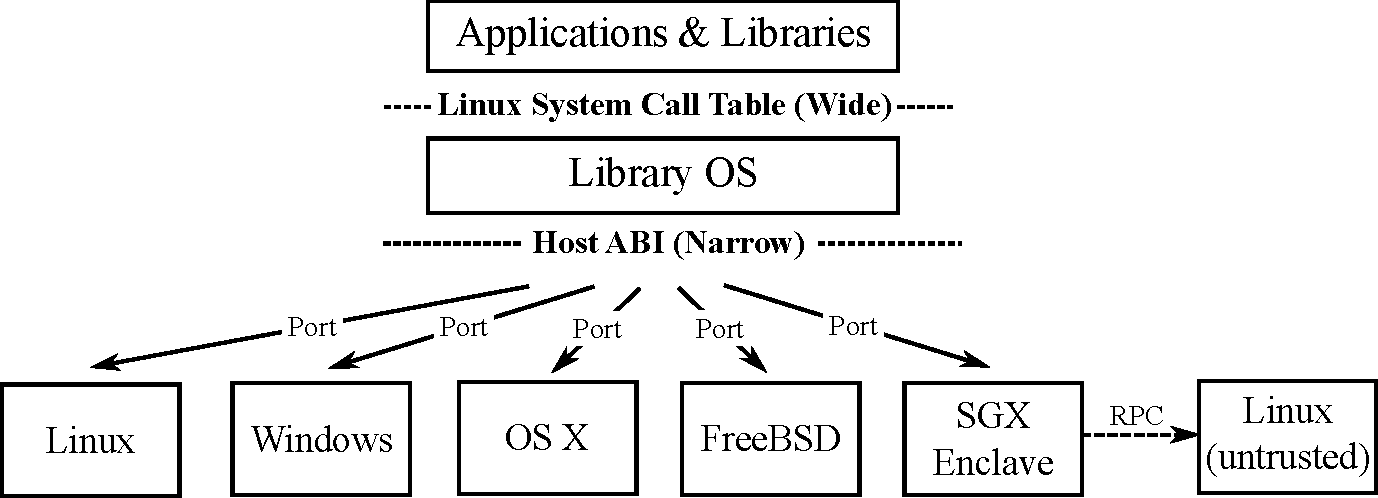
\includegraphics[width=30em]{porting.pdf}
\caption{Porting model of \graphene{}.}
%\vspace{-.1in}
\label{fig:overview:porting}
\end{figure}



\papersubsection{Platform Adaption Layers (PALs)}
\label{sec:overview:host:pal}


For each host OS or hardware, \graphene{} uses
a thin library called a {\bf platform translation layer (PAL)}
to translate among host interfaces.
%is loaded below the library OS, to translate each functions in \thehostabi{} to native system interfaces.
The main purpose of a PAL is to mitigate the semantic gap
between \thehostabi{} and
native host system APIs.
%The effort of PAL development is per host OS, whereas the library OS implementation is reusable on every hosts. %The simplicity of \thehostabi{} can be also estimated by the effort of implementing a PAL for each host.
By implementing a PAL on a new host OS or hardware,
users can reuse
the same \libos{} to run the same collection of unmodified Linux applications.
%To keep the porting effort low,
%the development of a PAL must be straightforward
%for average OS developers.
%to achieve with limited efforts.
%Based on the principle of porting simplicity, PAL development must be straightforward
%for average developers.







%The host ABI is defined for the simplicity of porting, as well as the sufficiency for implementing a library OS compatible to Linux.
%First of all, the number of host functions included in \thehostabi{}
%is much smaller than the number of system calls in a commodity OS such as Linux. 
\graphene{} currently contains PAL implementations for several popular OSes,
including Linux, \win{}, \osx{}, and FreeBSD.
%and \sgx{} with an untrusted Linux kernel.
Most of these OSes provide a POSIX-like system API similar to \thehostabi{}.
Due to the similarity, translating most of \thehostabi{} to one of the system APIs
are straightforward for average OS developers.
\Thehostabi{} is also much smaller than the actual POSIX API, making it extremely portable.



A part of \thehostabi{} may be challenging to port
on an OS,
due to unexpected system assumptions made by the OS.
For instance, \win{} does not support
fine-grained memory deallocation for de-privileged applications.
To implement system calls like \syscall{munmap} and \syscall{mprotect},
\graphene{} needs host ABIs to
deallocate or protect virtual memory pages at page granularity.
%A workaround is to change memory mappings at the physical page level,
%but will require running the \win{} PAL with root permissions.
%This type of porting challenges
%tends to be results of design decisions or assumptions made by OS developers.
%A \libos{} can potentially design
%different emulation strategies
%to compensate missing host abstractions.
A few host abstractions such as a bulk IPC feature are
optional to the host ABI;
if a host OS does not support these abstractions,
the \libos{} must fall back to alternatives. 

%In our experience, the development of a PAL is around ten thousand lines of code.

%For each port, the amount of code written for implementing \thehostabi{} is at the order of magnitude of thousands of lines of code, which is much more manageable than implementing a flat translation layer for system interfaces.


\begin{comment}
Based on the experience in \graphene{},
it is hard to ensure the portability of \thehostabi{} on every potential hosts.
%even a host ABI specialized for simplicity cannot guarantee to be portable on every hosts.
A host may simply lacks the functionality
for implementing a \hostapi{}.
The assumption is, maintaining the compatibility of \thehostabi{} poses a much less challenge than maintaining the whole system API.
Besides, the library OS may flexibly switch among emulation strategies
to compensate the absence of certain host abstraction.
As an example,
bulk IPC is optional in \thehostabi{} since its first definition,
due to the expectation
that implementing the feature may not be feasible on some hosts.
If bulk IPC is not available,
the library OS can fall back to RPC-based IPC, with a reasonable amount of performance penalty.
In the worst case, if there is no emulation strategies
to compensate for the absence of a \hostapi{},
user can predict the affected applications and avoid running these applications
on specific hosts. 
%at least users can predict whether an application will be affected and thus cannot run on certain hosts.
\end{comment}


%For a host OS that does not support ELF binaries, the PAL must follow the binary format which the host OS accepts, such as the Portable Executable (PE) format on \win{}.
%The PAL is the only layer in the user space which cannot be reused
%across different hosts. Besides the PAL, all of the other binaries in the user space are fully reusable, including the library OS, the supporting libraries, and the application executable.



%The host abstractions map to several common system calls in a commodity OS.
%For example, \funcname{StreamRead} and \funcname{StreamWrite} can directly map to the POSIX functions \funcname{pread} and \funcname{pwrite}, which are available in most OSes including Linux, BSD, \osx{}, and \win{}.
%More than half of the functions in \thehostabi{} can be counted toward this category.
%The rest of the host abstractions are either specific to Linux
%(e.g., TLS support),
%or belong to the POSIX functions that are not shared with commodity OSes
%(e.g., \funcname{mmap} on \win{}).
%The PAL emulates these host abstractions, using existing system interfaces available on the host OS, unless the software emulation is fundamentally impossible (e.g., restricted by the system interfaces), or too expensive (e.g., high overhead from copying data).



\papersubsection{Definitions and design principles}
 

\graphene{} defines \palcallnum{} calls in \thehostabi{} (also called \hostapis{}),
with a set of host abstractions
sufficient for \libos{} development.
%The host ABI defines the interaction between the library OS and a specific host.
%The \graphene{} library OS can be deployed on any ``host'' where \thehostabi{} has been ported.
This thesis defines
a {\bf host} of \thehostabi{}
to be an OS or hypervisor
which contains enough OS functionality for running a standalone application or virtual machine.
Most of the host targets in \graphene{}
are monolithic OSes,
including Linux, \win{}, \osx{}, and FreeBSD.
%which has defined a massive system API for programmability.
A monolithic OS 
usually contains a massive amount of system APIs,
which is sufficient for
implementing \thehostabi{}.


A special example of a host
is an \sgx{} (Software Guard Extensions) enclaves~\cite{intelsgx},
which
restricts OS functionality for security reasons.
The restrictions on \sgx{}
are results of a strong threat model
which distrusts any OS features except ones that are virtualized by the CPUs or migrated into enclaves.
The only way to obtain any missing OS features such as storage or networking
is to request through RPC (remote procedure call).
Requesting untrusted OS services through RPC also introduces new security threats that application developers tend not to anticipate~\cite{checkoway13iago,osdi16scone}.
Due to all the compatibility and security challenges discussed above,
this thesis uses \sgx{} as a representative example of a host
with unusual assumptions (e.g., threat models) and restrictions
compared to a monolithic OS.

%An innovative hardware abstraction like \sgx{} (software guard extensions)
%imposes unique assumptions and restrictions
%on a commodity OS,
%%creates a special host on top of Linux or \win{},
%%with unique interfaces and specifications regarding the host OSes.
%and thus creates a special host above the OS.

%If an OS has mutated or tweaked the interface for a hardware platform,
%such as an \sgx{} enclave 
%running on an untrusted Linux kernel,
%the combination of the OS (Linux) and the hardware platform (\sgx{}) is considered a specialized host.
%Especially, the \sgx{} port of \thehostabi{} faces several unique challenges,
%which will be discussed in Chapter~\ref{chap:sgx}.


\begin{comment}
%\fixme{each sentense should be a paragraph; starting the 2nd sentence}
\fixmedp{start with a strong opening stating the rationale}
The host ABI of \graphene{}
define functions needed from a host, in order to implement the library OS for reusing applications.
%to reuse an application and all its supporting libraries, including the \graphene{} library OS.
Each host of \graphene{} contains an OS and a hardware platform, either of which causes compatibility issues for running unmodified applications.
OS developers can port the library OS to a new host,
by simply reimplementing the narrowed host ABIs using abstractions available on the host.
%a new host platform.
%For each host which requires the compatibility for unmodified Linux applications, one only has to implement the narrowed host ABIs,
%instead of reimplementing the bloated, ``legacy'' system interfaces
%needed by the applications.
By implementing \thehostabi{}, OS developers skip the painful process of rebuilding the whole system interfaces of a commercial OS such as Linux.
The host ABIs strictly decouples the porting effort on the hosts from the compatibility feature for applications.
%The host ABIs decouple the OS development in the host and the implementation of compatibility for the existing Linux application.
What \thehostabi{} exposes is a simplified extended machine,
similar to a para-virtualization interface, capable of running the library OS as a lightweight virtual machine. % with compatibility against Linux applications.
%on which another layer of virtualization (i.e., the library OS) can be built to reproduce the compatibility for Linux.
\end{comment}


\begin{comment}
Two design principles drive the definition of \thehostabi{}s:
{\em simplicity} (i.e., easy to port on any hosts)
and {\em sufficiency} (i.e., containing enough OS functions for implementing a library OS).
The process of deciding \thehostabi{}s is comparable to
finding a ``pinch point'' within a OS implementation,
which can conveniently mediate a significant portion of OS execution paths for managing hardware abstractions.
%The two principles drive the development of \thehostabi{}s,
%The whole development of the \graphene{} library
%must be disciplined
%on extending \thehostabi{}s only when it is strongly required.
%of restraining extensions to \thehostabi{}s unless absolutely necessary.
The two principles
determine the soundness of the \graphene{} approach to improving compatibility
for any hosts.
\end{comment}


%%The host ABI is defined with partitioning in mind.
%\Thehostabi{} 
%determines a boundary which partitions several upper-level OS components, %, such as system calls and namespaces,
%into a library OS,
%%, as a dynamically-linked library which can be deployed
%%to various hosts.
%%The rationale behind the partitioning is based on the fact that not every OS component is equally important to compatibility, for applications which need to be ported across hosts.
%%When an OS is extended for a new hardware,
%%these OS components usually remain unchanged, or are predominantly reused.
%%Partitioning
%%into a library OS further guards these 
%in order to isolate the host idiosyncrasy. % on specific hardware. %any potential changes for adopting new hardware.
%%Similar isolation
%%exists in traditional OSes, but without partitioning:
%The strategy
%is also used in OSes:
%An example is the Linux virtual file system (VFS), an internal interface
%which encapsulates operations of file system drivers.
%%On the other hand,
%%drivers (e.g., drivers for file systems, block devices, or network cards)
%%and architecture-specific instructions
%%stay encapsulated in the host OS.
%%in the Linux kernels are usually encapsulated under a virtualized, in-kernel interface (e.g., the Linux virtual file system),
%%to simplify the development of the rest of the kernel.
%Similar to VFS,
%\thehostabi{} is intended
%to be a more ubiquitous interface,
%which encapsulates
%any host-specific behavior and semantic
%inside the host OS.
%%for encapsulating both OS and hardware idiosyncrasy on a wide range on hosts.
%%declares a ubiquitous system interface, to encapsulate both OS and hardware abstractions
%%for the library OS.




\Thehostabi{} shares several characteristics with a virtual hardware interface
exported by a hypervisor.
A generic, backward-compatible
virtual hardware interface
%a set of generic, virtual hardware,
%which the VM can control with the same drivers.
allows an unmodified OS kernel to run inside a virtual machine as on the bare metal.
%by exporting interfaces close to commodity hardware.
%To avoid additional porting effort, the virtual hardware are close to the typical commodity hardware.
%For instance, a virtual hardware interface
%usually includes a virtual NIC (network interface controller),
%such as the virtualized E1000 interfaces
%available in VMware workstation or QEMU.
%As a result, \thehostabi{} contains the
%typical OS features and interfaces, similar to the API of early UNIX systems.
The key difference between
a virtual hardware interface
and \thehostabi{}
is that \thehostabi{} does not target reusing a whole, unmodified OS kernel as a guest.
Instead, 
\thehostabi{} contains higher-level abstractions such as files and network sockets
to ensure portability on most host OSes.
The concept
of defining \thehostabi{}
with a customized guest OS (i.e., a \libos{}) running atop \thehostabi{} is similar to para-virtualization.
%\thehostabi{} expects the \libos{}
%to be rewritten and
%customized for \thehostabi{},
%similar to a 
%para-virtualizated VM.
%Compared to an actual para-virtualized VM,
A para-virtualized VM defines hypercalls as interfaces between a guest OS and a hypervisor.
Furthermore, \thehostabi{} avoids duplication of OS components
such as scheduler, page fault handler, file systems, and network stacks
between the host and \libos{}.
%Another difference is that \thehostabi{} is called by normal function calls, whereas para-virtualization relies on hypercalls.
To compare a VM and a \libos{} on a spectrum,
a VM reuses a whole OS on a wide, backward-compatible virtual hardware interface
whereas a \libos{} implements only system API components on a simplified host ABI.

The following paragraphs discuss the key design principles of \thehostabi{},
including porting simplicity, sufficiency for \libos{} development, and ease of migration.

\paragraph{Porting simplicity.}
%To reduce porting effort
%\thehostabi{}
%must be simple to port on a host OS or hardware.
To reduce porting efforts,
\graphene{} defines \thehostabi{}
using two strategies:
first, \graphene{} significantly reduces both the size and complexity of host OS features
that OS developers have to implement.
Effectively, \graphene{} avoids duplicated OS features and handling rare corner cases
on \thehostabi{}.
%The development of \graphene{} disciplinarily avoiding adding any functions to \thehostabi{},
%unless the library OS cannot internally implement an OS feature.
Second, the definition of \thehostabi{}
imitates common system APIs in a POSIX-like monolithic OS,
to directly translate most calls to
a few similar host abstractions.
%existing system calls or system library functions
%on each host.
%include functions which can be directly mapped to OS functions exported by the host.
%%the likelihood of finding similar features on the host, to be translated to functions in \thehostabi{}.
%The assumption that such a strategy is possible
%is based on
%the observation that
%%similarity of system interfaces is common among most OSes.
%similar OS functions, especially UNIX-style APIs,
%tend to commonly exist in most OSes.
%, to reduce the learning curve for programming applications.
For instance,
the stream APIs in \thehostabi{}, such as \palcall{StreamRead} and \palcall{StreamWrite}
are similar to
system calls like \syscall{read} and \syscall{write} exist on Linux, BSD, and POSIX API,
or \syscall{ReadFile} and \syscall{WriteFile}
on \win{}.
%with similar functionality and semantics.
%and 
%looks similar to \syscall{ReadFile} in \win{}, except the data types.
%The definition of \thehostabi{}
%is based on observations of the system interfaces in some of the important hosts,
%including Linux system calls and \win{} API.
%exported by the targeted hosts,
%and defines the functions in \thehostabi{}, to be easily translated to the native system interfaces.
%The host ABI is essentially a subset of the common features from every potential hosts.
%We expect %\thehostabi{} defined with simplicity in mind
%to be straightforward to port on most hosts,
%Most functions in \thehostabi{} can be easily translated to host system interfaces
%in various styles.
As the rest of this thesis proves, porting \thehostabi{} is straightforward
on most monolithic OSes.

%For example, \thehostabi{} defines \syscall{StreamRead} and \syscall{StreamWrite} for accessing I/O streams, similar to .
%xcept some nuanced details like order of parameters.


% by including OS functions , such as \syscall{FileRead} and \syscall{FileWrite}, similar to the Linux system calls, \syscall{pread} and \syscall{pwrite}.




\begin{comment}
The simplicity of \thehostabi{}s requires retaining a minimalist design of host functions. %, based on typical OS services for managing hardware.
%\graphene{} reduces the host functions
%to the bare minimum.
The host ABIs should only contain operations that
are absolutely necessary for requesting external hardware abstractions.
%A way to simplify \thehostabi{}s is to move host functions into the library OS
%and to replace them with wrappers consisting of other host functions.
Any functions that can be partially or wholly implemented inside the library OS
should be further simplified, or even removed from \thehostabi{}s.
%---in other words, whether \thehostabi{}s can be further reduced.
Moreover, \thehostabi{}s have to be simple enough to implement on
most hosts;
%In the simplest host ABIs, none of the host functions shall be able to internally implement the behavior of another host function,
%or the definition of \thehostabi{}s is further reducible.
that is, \thehostabi{}s should contain only OS functions that are commonly offered on
most hosts.
The host ABIs are close to simplified UNIX interfaces,
such as reading or writing a file or an I/O device as a byte stream,
or creating a virtual memory mapping.
%the most common OS functions
%offered on most of the potential hosts,
For most hosts,
implementing \thehostabi{} should be as straightforward as redirecting the functions to the closest host system calls.
%such as the Linux system calls or the \win{} APIs.
For example, the functionality of \syscall{StreamRead} and \syscall{StreamWrite} in \thehostabi{}s can loosely match with
\syscall{read} and \syscall{write} in Linux,
or \syscall{ReadFile} and \syscall{WriteFile} in \win{}.
%This thesis also evaluates the simplicity of \thehostabi{}s by counting the lines of code used to implement \thehostabi{}s on each host platforms.
Since most OSes have inherited a similar design from UNIX,
it is fair to assume finding
comparable OS functions %host platforms
to \thehostabi{} would be reasonably easy.
%fair to assume that \thehostabi{}s 
\end{comment}



\paragraph{Sufficiency for \libos{} development.}
%\Thehostabi{} defines
%the host abstraction available for a \libos{} to access host hardware abstractions.
To develop a \libos{} with compatibility against a wide range of applications,
\thehostabi{}
%are demonstrated by the fact that
%the exported host functions 
contain any OS abstractions that the \libos{} cannot easily emulate.
%and a full-function library OS is implemented on top of them.
For most hosts,
the host OS abstractions
%can be categorized into five types:
include
process creation, memory management, and I/O (typically, files and network connection)~\cite{dhamdhere2007os-textbook}.
%Besides security and protection,
%the definition of \thehostabi{} is closely related with hardware management,
%and offers the most basic abstractions for each category of OS functions.
%managing specific types of hardware,
%and each contain a few basic abstractions
%which can be expanded into other system interfaces.
%For example, the basic OS functions for memory management include
%allocating (\syscall{VirtMemAlloc}),
%protecting (\syscall{VirtMemProt}),
%and deallocating (\syscall{VirtMemFree}) memory regions. % at certain granularity
%(usually in pages).
%These basic functions can be used to implement other forms of memory allocation,
%such as growing heaps with \syscall{brk}
%or allocating thread-private stacks.
%The definition of the \drawbridge{} host ABI is a hint, for creating a list of host abstractions necessary for the library OS, including streams, memory, threads, and processes. 
%If \thehostabi{}s are insufficient for implementing certain system interfaces, one may extend \thehostabi{}s with the missing functions,
%with the discipline to retain the simplicity of \thehostabi{}s.
%The extension to \thehostabi{}s must be d, to keep the extension minimal, and to avoid adding redundant functions.
%The implementation of the \graphene{} library OS demonstrates that
%\thehostabi{} is sufficient for implementing significant portion of Linux system calls.
For each type of abstractions,
a monolithic OS may define several variants of system APIs with similar functionality.
For instance, Linux provides two system calls, \syscall{mmap} and \syscall{brk}, both for memory allocation in a process.
\syscall{mmap} allocates larger memory regions with page granularity,
whereas \syscall{brk} simply grows a single, continuous heap space for more fine-grained allocation.
Many applications such as GCC~\cite{gcc}
switch among system API variants in case one of them is unavailable on certain OS distributions.
This thesis shows that,
by adopting only the semantics of one of these similar APIs or abstractions, the host OS can stay simple with
the \libos{} emulating the rest of APIs.
For instance, \thehostabi{} includes \syscall{VirtMemAlloc}
as a similar feature as \syscall{mmap},
which is sufficient to emulating both \syscall{mmap} and \syscall{brk}.



\graphene{} defines \thehostabi{} partially based on
\drawbridge{},
a library OS for single-process \win{} applications.
The host ABI of \drawbridge{} 
contains 36 functions,
%demonstrates that its host ABI is sufficient
%for running a library OS in which 99.7\% of code comes from the \win{} 7 source.
%The host ABIs of \drawbridge{} are later extended
%for running a Linux-based library OS called Bascule~\cite{baumann13bascule}.
and several works have ported the host ABI to different hosts,
including \win{}, Linux, Barrelfish, and \sgx{}~\cite{porter11drawbridge,baumann14haven,mssql-on-linux,baumann13bascule}.
%and is capable of running a library OS for single-process, Linux applications, with a few host ABI changes~\cite{baumann13bascule}.
%ill loads and links the rest of application binaries, just like the native Linux loader (i.e., \code{ld.so}).
%\graphene{} takes the high-level definitions of the \drawbridge{} and Bascule host ABIs, and customizes for general-purpose Linux applications and a wider range of hosts. 
Although running \win{} and Linux applications may face
a different set of challenges,
the nature of their APIs is mostly similar, with a few exceptions.
During the development of \graphene{}, developers found the occasions in which
the host ABI of \drawbridge{}
is not sufficient to address Linux-specific challenges
and decide to extend \thehostabi{}.
Section~\ref{sec:overview:host:abi} and Chapter~\ref{chap:abi}
will further discuss the Linux-specific extensions of \thehostabi{}.


\paragraph{Migration.}
The \graphene{} library OS shares several features of VMs, including checkpointing and migrating a running application.
Migrating a process is also the key to emulating copy-on-write forking,
on a host without physical memory sharing (e.g., \sgx{}).
A hypervisor checkpoints and migrates a VM by snapshotting the VM states above a stateless virtual hardware interface. % as a clean boundary for snapshotting the application and OS state.
\Thehostabi{} is also defined to be statelessness,
by ensuring any states in the hosts to be temporary and reproducible to the applications and \libos{}.





\papersubsection{The \hostapis{}}
\label{sec:overview:host:abi}


%\fixmedp{the beginning doesn't capture the whole paragraph.}
%The host ABI shares several common abstractions with production OSes.
%The functions in \thehostabi{}
%define the basic features needed from the hosts, to run the library OS.
%The definition of the host functions
%should be unsurprising to average OS developers,
%making the implementation on a new host to be fairly straightforward.
%The host ABI reflects the common functionality of most OSes, including Linux and \win{}.
%Although the same OS abstractions may be defined
%as different idiosyncratic system interfaces on each host OSes,
%\graphene{} takes into consideration of porting the host functions to either OSes, in the most effortless way possible.





%fixmedp{give more of the background}
Table~\ref{tab:overview:abi} lists the \palcallnum{} calls defined in \thehostabi{}:
%Among these \hostapis{}, 
25 calls are inherited from the \drawbridge{} host ABI,
including functions to managing I/O (e.g., \palcall{StreamOpen}), memory allocation (e.g., \palcall{VirtMemAlloc}), scheduling (e.g., \palcall{ThreadCreate}), and several miscellaneous functions (e.g., \palcall{SystemTimeQuery}).
%Most of the host functions only affect the OS or hardware states
%related to the process itself.
%For example, \syscall{VirtMemAlloc} can only allocate memory in the calling process,
%and cannot affect other processes running in parallel.
%Only I/O streaming functions export states to the host OS, and share states with other processes or library OSes.
14 calls are added by \graphene{}, to implement Linux-specific features.
For example, unlike \win{} or \osx{}, Linux %The host ABI is also complemented with several Linux-specific abstractions, such as
delivers hardware exceptions to a process as signals.
Linux also requires 
the x86-specific segment registers (i.e., FS/GS registers)
to determine the location of thread-local storage (TLS), which can be hard-coded in application binaries by a compilation mode of GCC.
On \win{} or \osx{}, the x86-specific segment registers are mostly ignored, and even frequently reset to eliminate attack vectors.
%The host ABI contains host functions (), which can be directly called from the library OS. \graphene{} shows that \thehostabi{} is sufficient to implementing a large portion of the Linux system calls.
%These functions are not defined in \drawbridge{}, the \win{}-based library OS,
%because these abstractions do not exist in \win{}.
%The \drawbridge{} host ABI does not contain exception delivery because the feature is
%not commonly used in \win{} applications.
%Moreover, the x86 segment registers cannot be modified in \win{}
%because the OS assigns fixed values to these registers
%for the whole execution.
%Although \drawbridge{} excludes these abstractions, Bascule extends \thehostabi{} to include similar functions,
%demonstrating that the extension is indeed necessary.
\graphene{} discovers these abstractions as a necessity for implementing a rich Linux \libos{}.



\begin{table}[htp!]
\centering
\input{abi-table}
\caption{An overview of \thehostabi{} of \graphene{}. The ones marked with the symbol $\dagger$ are introduced in the initial publication of \graphene{}~\cite{tsai14graphene} or later extended for this thesis. The rest are inherited from \drawbridge{}~\cite{porter11drawbridge}.}
\label{tab:overview:abi}
\end{table}

%The interfaces, as part of \thehostabi{}, which access these host abstractions, are ultimately simplified to reduce the porting effort on each host.
%Unlike the system interfaces in the OS, \thehostabi{} does not prioritize backward compatibility. Therefore, \thehostabi{} includes only the minimum interfaces that the library OS needs to interact with the host. The host ABI does not have to include any of  the legacy system interfaces from a production OS, let alone preserving different flavors of system interfaces for backward compatibility.



\graphene{} introduces five calls for 
remote procedure call (RPC) between \libos{} instances
in a multi-process application.
\graphene{} simplifies porting multi-process abstractions
on each host OS
to implementing RPCs.
The basic RPC abstraction is 
a pipe-like RPC stream for message passing between processes.
To improve performance,
%RPC is critical for implementing the coordination of OS states
%across library OS instances.
%The basic form of RPC in \graphene{} is a pipe-like RPC byte stream, which a library OS can simply use to send messages.
%It is a common design choice
%to implement inter-process coordination through message-passing
%instead of shared memory, especially for hardware platforms that do not guarantee memory coherence~\cite{baumann09barrelfish}.
%A problem to the message-passing approach is the significant overheads
%on frequently exchanging distributed OS states.
\thehostabi{} defines an optional, bulk IPC abstraction
to send large chunks of virtual memory
across processes.
%The bulk IPC feature works similarly as sending the memory through RPC streams,
%but is much faster because it avoids copying memory in the host.


%for host platforms that urgently require lowering the RPC overheads.
%Another extension is for
%%\funcname{StreamSendHandle} and \funcname{StreamRecvHandle}
%delegating opened stream handles to another process, through a connecting pipe.
%The feature is similar to sending file descriptors
%through UNIX sockets in Linux, and is used to share opened network sockets with the \syscall{fork}'ed processes.
%%Another RPC abstraction is a bulk IPC channel; a process can use \funcname{PhsyicalMemoryCommit} to commit a large chunk of memory to a bulk IPC channel, which \funcname{PhsyicalMemoryMap} can map into another process, as copy-on-write. The library OS uses bulk IPC as an optimization to \syscall{fork}.
%Despite that either of the RPC primitives
%is not necessary easy to implement on every hosts, the inclusion of these host functions is completely optional, and the library OS can always fall back to the message-passing approach.



%All the host functions are designed to appear as ``stateless''
%as possible to the library OS.
%Being stateless to the library OS means that
%a host function does not preserve any permanent state of certain host abstraction.
%A stateless function can recover
%from disconnection of the library OS, and be reconnected at any timing.
%The host functions can maintain temporary bookkeeping for the convenience of porting,
%but should not assume the bookkeeping states to be permanent.
%The principle of defining all the host functions to be stateless
%is primarily for two purposes:
%{\em migration} and {\em security isolation}.
%For migration, the fact that the library OS can disconnect freely from the host functions simplifies the implementation of the migration feature.
%Migration is also an important foundation to implementing \syscall{fork}, because the cloned process need to receive a snapshot of the parent process.
%For security isolation, 
%a stateless host function is easier to check,
%because the security monitor only has to verify each instance of host function calls,
%instead of tracing multiple host functions over a longer period of time.

%the functions to access each host abstraction must appear \fixmedp{clarify `stateless'} stateless to the host, except for the handles to identify the resources. Each call to the host functions is independent. The arguments given for each call must be always be absolute values, instead of relative values.
%For example, the offset given to \funcname{StreamMap}, \funcname{StreamRead}, and \funcname{StreamWrite} (if the opened handle is a file) are offsets from the beginning of the file, and thus are irrelevant to how many bytes that are previously written or read.
%When enforcing isolation rules, the host OS can check the arguments of each calls to the host functions, independently and atomically.


%A host ABI (application binary interface) has to define the convention of application binaries, including the binary format and the linking procedure, as well as a set of  system interfaces.
%The host ABIs contain a minimal loader which recognizes a basic version of the ELF (Executable and Linkable Format), just enough to compose a binary of the library OS.
%The very initial loading procedure as part of \thehostabi{}s only loads a clean library OS instance.
%Each host of \graphene{} is supposed implement a minimal dynamic loader,
%which can load the \graphene{} library OS binary in ELF.
%The library OS then completes the dynamic loading procedure,
%by directly loading the Linux native dynamic loader (i.e., \code{ld.so}), and indirectly loading the rest of the application binaries.







\papersubsection{Host-enforced security isolation}
\label{sec:overview:host:security}


To target multi-tenant environments, 
\graphene{} enforces strong security isolation between mutually-untrusting applications running on the same host.
The security isolation of \graphene{} is comparable to running each application
in a VM or a container.
Just as a virtual hardware interface isolating each VM,
\thehostabi{} also enforces security isolation between library OS instances.
%according to the trust model of the applications.


On a trusted host OS,
\graphene{} delegates security isolation as a host-level feature.
The library OS and the application must mutually trust each other, due to lack of internal privilege separation in a process.
%The host ABI also separates API implementation
%from security isolation.
%To ensure isolation, each host must restrict access from the applications or the library OS, to any unauthorized host abstractions.
On each host, a reference monitor enforces security isolation policies, by access control on OS abstractions sharable among processes, including files, network sockets, and RPC streams.
%The host-level security isolation is orthogonal to API complexity.
Separating security isolation from API implementation simplifies security checks
for applications that only require
complete protection from other tenants.
%based on monitoring the references to host resources and rejecting authorized resource access.
%to the host abstractions.





%\graphene{} reduces the attack surface exposed to applications
%by restricting access to the host kernel ABI 
%and prevents access to unauthorized system calls, files, byte streams,
%and network addresses with a \emph{reference monitor}.
%The host kernel ABI exported by the \pal{} heavily 
%limits the ability of a \graphene{} application to interact with the rest of the system;
%any external interactions are further mediated by a reference monitor.
%Unlike a typical Linux system, \graphene{} applications cannot interact with shared 
%system daemons or other shared system resources.
%As a result, \graphene{} enforces security isolation similar to running applications in separate VMs---even
%applications that span multiple processes.


In \graphene{},
one or multiple processes of the same application run in a {\bf sandbox}.
Multiple library OS instances coordinate
in a sandbox
to present a unified OS view
to the application.
%As the library OS instances can coordinate shared OS states using simple RPC streams,
The design simplifies the enforcement of security isolation for multi-process abstractions.
\graphene{}
uses the reference monitor to block RPC streams across the sandbox boundary,
stopping applications in different sandboxes from accessing multi-process OS states.
%\graphene{} contributes a multi-process security model 
%based on the abstraction of a \emph{sandbox},
%or a set of mutually trusting processes.
%If a reference monitor exists, the reference monitor permits the processes within the same sandbox to communicate and exchange RPC messages, but disallows cross-sandbox communication.
The current design focuses on security isolation, although we do expect to extend the design for more sophisticated policies
in the future.

\begin{comment}
The only host abstractions that are shared across processes and must be mediated by the host for isolation are files, network sockets, and RPC streams
--- all other allowed host ABI modify only local process state, such as VMAs and threads.
%Thus, the reference monitor need only mediate file access, socket and RPC stream creation.
%an unprivileged daemon
%as well as extensions to the App\-Armor LSM~\cite{apparmor},
%which checks file and socket policies in the kernel.
%, reducing context switching overhead
%and the risk of race conditions~\cite{garfinkel03traps}.
In order for the reference monitor to restrict file access, socket and RPC stream creation,
each application includes a {\em manifest file}~\cite{hunt07rethink},
which describes a {\tt chroot}-like, restricted view of the local 
file system (similar to Plan 9's unioned file system views~\cite{pike90plan9}),
%including read-only shared files,
as well as {\em iptables}-style~\cite{iptablesman} network firewall rules.
To facilitate sharing read-only libraries, a manifest may specify a file system view which combines several different sub-directories of the local file system, and can prevent writing to files or directories.


For example, the \graphene{} reference monitor on the Linux host is implemented using \syscall{ioctl} to a special device (\code{/dev/graphene})~\fixme{a prospective design}.
A process is restricted by the Linux BPF-style system call filter, or the SECCOMP filter~\cite{seccomp}, to use \syscall{open} to access any files, or to \syscall{connect} or \syscall{bind} to any sockets.
It must use the \graphene{} special device to open or create streams, so the file paths or network addresses can be checked against the sandbox rules. The kernel module as the driver of the \graphene{} special device can coexist with any Linux Security Module (LSM), such as AppArmor~\cite{apparmor} or SELinux~\cite{selinux}.


When a new process is launched by the host, it begins execution in a new sandbox.  
Child processes may either inherit their parent's sandbox, or can be started in a separate sandbox---specified by a flag to the host abstractions of process creation.
A parent may specify a subset of its own file system view 
when creating a child, but may not request access to new regions of the host file system. 
%The restrictive policy enforced on the child will be written in a new manifest file generated by the parent, and the policy will be checked by the reference monitor.
The child may also issue an {\tt ioctl} call to 
dynamically detach from the parent's sandbox. The reference monitor prevents byte stream creation across sandboxes.
%among picoprocesses
%that are not in the same sandbox.
%and restricts external connections to remote URIs according to firewall rules in the manifest.
When a process detaches from a sandbox, effectively splitting the sandbox, the host must closes all RPC streams that could bridge the two sandboxes.
\end{comment}



\paragraph{Threat model.}
For most hosts, application trusts the host OSes as well a \libos{} instances in the same processes.
For multiple processes inside a sandbox,
the \liboses{} in these processes
also trust each other.
Applications or \liboses{} are not trusted by the host OSes or processes outside of the sandboxes.
Applications and \liboses{}
can become the adversary to the host OS,
by exploiting vulnerabilities on \thehostabi{}.
%the \graphene{} design reduces the attack surface between the hosts and the library OS instances, to defend against a malicious application.

%On a host with a reference monitor, the host OS and the reference monitor are both trusted, to mediate all system interfaces used to implement \thehostabi{}. The host must check all access to any abstractions with effects outside of a process's internal state, such as an opened file, or a connected network socket.
%Processes inside the same sandbox mutually trust each other. The adversary can run arbitrary code inside of one or more processes within one or more sandboxes.
%The adversary can control all code in its processes, including the library OS and the host-specific PAL.
%{\tt libLinux} and the \pal{}. 
%We also assume a trusted reference monitor process running on the host kernel that 
%launches \graphene{} applications and mediates all system calls with external effects,\fixmedp{define precisely}

%\graphene{} ensures that %The key security property the \graphene{} design upholds is that 
%the adversary cannot interfere with any victim picoprocesses
%in a separate sandbox.  
%The \graphene{} sandbox design ensures strict isolation: 
%if the only shared kernel abstractions are byte streams and files, 
%and the reference monitor ensures
%there is no writable intersection between sandboxes,
%the adversary cannot interfere with any victim picoprocess.


The threat model of \graphene{} on \sgx{}
contains the adversary from other hosts but excludes
the host OS, hypervisor, and any hardware except the CPU from its trusted computing base (TCB).
An untrusted OS or hypervisor
potentially has lots of opportunities to invade applications or VMs,
using Iago attacks~\cite{checkoway13iago}.
The challenges of porting \graphene{} to \sgx{} is not limited to resolving the compatibility issues of enclaves but also defending applications and \liboses{} against untrusted host OSes.







%%% The only processes allowed to run as standard kernel processes (non-\graphene{}) 
%%% are the reference monitor and
%%% system administration utilities that need more kernel interfaces than the \pal{} ABI provides.
%%% Ensuring that a collaborating picoprocess correctly implements
%%% some function (such as receiving a signal),
%%% as well as preventing exploitation of vulnerabilities in picoprocesses
%%% are beyond the scope of this work.

%\graphene{} reduces the system attack surface of the host, but does not change the size of its
%trusted computing base; however, reducing the effective system call table
%size of a picoprocess does facilitate adoption of a smaller host kernel,
%which we leave for future work.





\papersection{Security isolation}
\label{sec:linux:security}

\issuedone{1.1.d}{Describe the security isolation story for Linux hosts}
\graphene{} separates OS features from security isolation.
This section explains the Linux host design for isolating mutually untrusting applications, with a reduced attack surface for protecting Linux kernels.
The discussion starts with the security guarantees and threat model, followed by the technical details of security isolation on a Linux host.



\papersubsection{Goals and threat model}

The security isolation model of \graphene{} ensures that mutually-untrusting applications cannot interfere with each other.
A goal of \graphene{} is to provide security isolation with comparable strength as
running applications in separate VMs.
When running two unrelated applications on the same machine,
the security requirement
of the OS involves not only blocking unauthorized access under normal circumstance,
but also preventing an application
from maliciously exploiting OS vulnerabilities to attack the other application.
Because a modern OS, such as Linux or \win{}, contains a rich of features and APIs,
it is difficult to eliminate OS vulnerabilities
or even just to verify whether an OS contains any vulnerabilities. 
A Linux container~\cite{lxc}
does provide a separate OS view for each application,
but still relies on the correctness of the whole Linux kernel to enforce security isolation.
On the other hand, a VM or a \libos{}
isolates the whole OS kernel or a part of the kernel in an unprivileged guest space
for each application.
The security isolation model prevents
any vulnerabilities inside the VM or the \libos{} from compromising the host kernel and other applications.



\graphene{} enforces security isolation %between applications
by separating 
backward-compatible OS features from security mechanisms.
A Linux kernel exports a wide range of system calls,
either as a legacy of previous kernels or as new programmability features. % of newer kernels.
By implementing OS features in a \libos{},
\graphene{} reduces the attack surface of a Linux kernel
to a small amount of system call corner cases.
%to implement \thehostabi{}.
%If a machine only runs applications in \graphene{},
%a Linux developer can try to carve out a minimal Linux kernel, containing only features needed by the Linux PAL.
A reduced attack surface
eliminates majority of execution paths inside a Linux kernel in which a malicious application can explore for vulnerabilities.
The complexity of Linux features and APIs exported by a \libos{} is unrelated with the attack surface of the host kernel,
unless the \libos{} asks for additional \hostapis{}.
A Linux developer can even carve out a minimal Linux kernel with only the features needed by the Linux PAL,
similar to shrinking a Linux kernel to a microkernel.
Otherwise, \graphene{} depends on the host security mechanisms to restrict a \libos{} from accessing unauthorized system calls and resources upon an unmodified Linux kernel.





The Linux PAL installs a {\bf system call filter} and a {\bf reference monitor}
for restricting the system calls, files, RPC streams, and network addresses
accessed by a \picoproc{}.
The Linux PAL requires \hostsyscallnum{} system calls in total
for implementing both required and optional \hostapis{}.
A system call filter, such as the Linux \seccomp{} filter~\cite{seccomp},
can restrict the system call access of an application
to only a small subset of all the system calls, with additional constraints on the parameters and optional flags permitted for each system call.
%The system call filter
%forbids an application from invoking any system calls
%that will interfere other \picoproc{} or increase the risk of exploitation in the host kernel.
A reference monitor further examines the arguments of permitted system calls to restrict the host resources accessed by an application, based on security policies configured in a manifest file~\cite{hunt07rethink}.
The system call filter and the reference monitor
significantly limit the ability of an untrusted \graphene{} \picoproc{} to interfere with the rest of the system,
preventing the risk of exposing any unknown vulnerabilities
on a kernel path never exercised by the system call footprint of \graphene{}.



\graphene{} contributes a multi-process security model 
based on a {\bf sandbox},
or a set of mutually-trusting \picoprocs{} running inside an isolated container.
The reference monitor permits picoprocesses within the same sandbox
to communicate over RPC streams,
allowing the \libos{} to share and coordinate any states
to create an unified OS view.
If two \picoprocs{} belong to different sandboxes,
the reference monitor will block any attempt of connecting RPC streams
between the \picoprocs{}
The access control over RPC streams
enforces an all-or-nothing security isolation model:
either two \picoprocs{} are in the same sandbox and share all the \libos{} states; or they are separated in two sandboxes and share nothing.
Even though the \libos{} instance can span its state across multiple \picoprocs{},
a host kernel needs not to examine the accesses to shared \libos{} states, but still enforces security isolation between sandboxes.




Files and network addresses
are the only host resources allowed to be shared across sandboxes,
using well-studied, explicit rules.
For sharing files, the reference monitor restricts the file access of a \picoproc{}
within a few host file or directories,
creating a restricted view of the local file system
(close to Plan 9's unionized file system views~\cite{pike90plan9}).
The file rules
in a manifest are similar to the policies of a {\bf AppArmor profile}~\cite{apparmor};
for each permitted file or directory,
a developer specifies the URI prefix and the permitted access type, either as read-only or readable-writable. %, within the target file or directory.
For sharing network addresses,
the reference monitor restricts a \picoproc{} from connecting through a local address or connecting to a remote address,
using {\bf iptables-like firewall rules}~\cite{iptablesman}.
Each network rule in a manifest
specifies the local or remote IP address and port range that a \picoproc{} is permitted to bind or connect a network socket.
The rules in a manifest file
specify a minimal list of files and network addresses that a \picoproc{} needs to access, and are largely based on existing security policies (e.g., AppArmor profiles, firewall rules).





\paragraph{Threat model (details).}
When running on a normal Linux host (without \sgx{} or other security hardware), \graphene{} assumes a trusted host kernel and reference monitor.
All the components inside the kernel space, including the \code{gipc} kernel module for bulk IPC, and the reference monitor,
are fully trusted by the other parts of the host kernel and the \graphene{} \picoprocs{}.
%which mediates all system calls with effects outside of a picoprocess's address space,
%such as file {\tt open} or network socket {\tt bind} or {\tt connect}.
On the other hand,
the host Linux kernel does not trust the \picoproc{}, including the Linux PAL, a \thelibos{} instance, \glibc{}, and the application.
The system call filter and reference monitor
initialized before an application starts running
defend the whole host kernel from malicious system calls invoked by a \picoproc{}.



All the components running within a \picoproc{}, including the Linux PAL, the \libos{} (\thelibos{}), \glibc{} libraries, and the application,
mutually trust each other. %, because all these components
%execute in the same guest address space.
Without internal sandboxing, the Linux PAL or \thelibos{}
cannot protect its internal states or control flows from an application.
Although some scenarios might require protecting the PAL or \thelibos{}
from the application,
\graphene{} only restricts the adversary
within a \picoproc{};
in other word, an adversary
only compromises the \libos{} in the same \picoproc{},
but can never interfere the host kernel 
or other unrelated \picoprocs{}.



For a multi-process application,
\graphene{} assumes that the \picoprocs{} 
%launched by the same application instance
running inside the same sandbox
trust each other and that all untrusted code run in sandboxed \picoprocs{}.
\graphene{} assumes the adversary can run arbitrary code inside
one or multiple \picoprocs within a sandbox.
The adversary can exploit any vulnerabilities in the \libos{}
or IPC protocol,
to propagate the attack to other \picoprocs{}.
\graphene{} ensures that
the adversary cannot interfere with any victim \picoprocs{}
in a separate sandbox.
A sandbox strictly isolates the coordination of \thelibos{} instances;
%if the only shared kernel abstractions are byte streams and files, 
the reference monitor ensures
that there is no writable intersection between sandboxes, so that
the adversary cannot interfere with any victim \picoprocs{}.


%%% The only processes allowed to run as standard kernel processes (non-\graphene{}) 
%%% are the reference monitor and
%%% system administration utilities that need more kernel interfaces than the \pal{} ABI provides.
%%% Ensuring that a collaborating picoprocess correctly implements
%%% some function (such as receiving a signal),
%%% as well as preventing exploitation of vulnerabilities in picoprocesses
%%% are beyond the scope of this work.

\graphene{} reduces the attack surface of the host Linux kernel, but does not change the trusted computing base; however, reducing the effective system call table size of a \picoproc{} does facilitate adoption of a smaller host kernel.
This thesis leaves the creation of a smaller host kernel for future work.

\papersubsection{System call restriction}
\label{sec:linux:security:syscall-restriction}


\graphene{} reduces the host ABI to \palcallnum{} calls
and the Linux system call footprint to \hostsyscallnum{} system calls.
To reduce the effective attack surface to a Linux host,
the Linux host restricts a \picoproc{} from accessing any system calls that are not part of the ordinary footprint of a Linux PAL.
The system call restriction on Linux focuses on blocking most of the system calls
that interferes with other processes.
The remaining permitted system calls with external effects are checked by 
the reference monitor (see Section~\ref{sec:linux:security:ref-monitor}).
 
%% dp: Meh
%%% Any picoprocess implementation 
%%% must restrict access to the host system call table,
%%% generally by blocking system calls in the host kernel~\cite{porter11drawbridge}
%%% or using {\tt ptrace}~\cite{xax}.


%The \pal{} is a host-provided library which implements \palcalls{} generic kernel ABIs,
%implemented using 
%These native system calls include {\tt ioctl} with 5 opcodes exclusively used by \graphene{} kernel extensions.

%This section describes how we adapt recent Linux sandboxing techniques 
%to \graphene{}.


%all allowed system calls with potentially external effects.

%%% For instance, an attempt to open a file will be checked by the reference monitor
%%% to see if the file is included in the sandbox definition, specified in the manifest
%%% with required permissions.
%%% Once the file handle is open, the \pal{} is then allowed to issue an {\tt mmap} or {\tt read}
%%% on the handle, as this operation can only affect the picoprocess address space
%%% or  file, which was already checked.

%Because the \pal{} is in the same address space as the application code, it is not
%trusted to enforce any security policies, and our threat model assumes that
%the \pal{} can be compromised by the adversary.
%Thus, the host kernel 
%only permits system calls that appear in the \pal{}'s source code and, through the reference monitor, further inspects calls that can have external effects.

%\begin{figure}[t!]
%\centering
%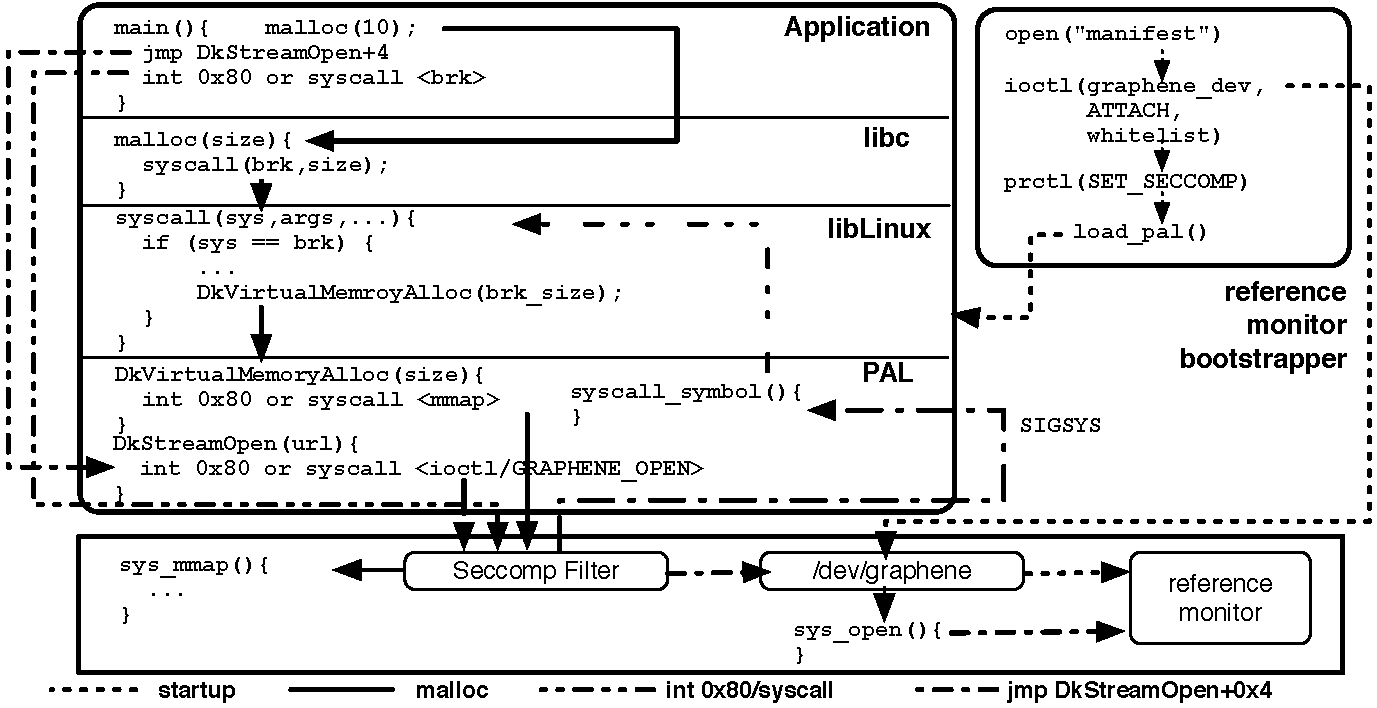
\includegraphics[width=\linewidth]{syscall-restriction.pdf}
%\footnotesize
%\caption[System call restriction approach in sysname{}]
%{System call restriction approach. The reference monitor loads policies into the LSM at startup.  A \graphene{} application requests OS services in three different ways. 
%In the normal case (first line of {\tt main}), {\tt malloc} is invoked causing the invocation of {\tt brk} ({\tt libLinux}) and {\tt mmap} in the \pal{}. In the second line, the application jumps to an address in \pal{}, which is permissible.
%Files are accessed through {\tt ioctl} to {\tt /dev/graphene} and checked by reference monitor.
%The third line invokes {\tt brk} with an {\tt int} instruction, which is redirected to the {\tt libLinux} function.}
%\label{fig:graphene:syscall-restriction}
%\end{figure}



\issuedone{1.3.d}{Extend the discussion of \seccomp{} filter}
\graphene{} restricts the host system calls 
using a \seccomp{} %(SECure COMPuting)
filter~\cite{seccomp}, a feature introduced in Linux 2.6.12.
% a recent Linux system call filtering mechanism, called 
A \seccomp{} filter allows a Linux process to install an immutable Berkeley Packet Filter (BPF) program
that specifies allowed system calls, as well as specifies
the consequence of invoking certain system calls, such as creating a \code{ptrace} event or raising a \code{SIGSYS} signal.
The BPF grammar is rich enough to filter scalar argument values,
such as only permitting specific opcodes for \syscall{ioctl},
as well as filter certain register values, such as blocking system calls from program counters (i.e., \code{RIP} register values) outside of the Linux PAL.
%This feature is particularly salient in the case of {\tt ioctl},
%where the \pal{} uses 5 out of over 400 opcodes for our bulk IPC module and sandbox creation;
%our BPF rules will block any other {\tt ioctl} opcode.
The current \seccomp{} filter installed by the Linux PAL contains \seccomplines{} lines of straightforward BPF macros.  %Experiments show that adding more precise argument checks has no significant impact on system call latency.
Once a \seccomp{} filter is installed in a process,
the filter intermediates
every system calls from the process and its future children, and guarantees the processes can never bypass the restriction.
The Linux PAL uses \code{SIGSYS} signals to capture rejected system calls,
and can either terminate the whole application or
redirect the system call to \thelibos{}.
The consecutive steps of system call redirection are described in Section~\ref{sec:libos:syscall-redirection}.



Developing a \seccomp{} filter presents several technical challenges.
First, a filter must restrict consecutive \picoprocs{}
to install a new filter the reverts the system call restriction.
%A \seccomp{} filter is installed using the \syscall{prctl} system call, so
Blocking the \syscall{prctl} system call in a \seccomp{} filter will prevent further installation of \seccomp{} filters.
Second, the BPF grammar can only filter certain values or ranges of a register.
The filter needs to
ensure that only the Linux PAL can invoke system calls;
however,
for satisfying the dynamic loading behavior of \thehostabi{},
the Linux PAL
is built as a shared library loaded at an address randomized by the Linux ASLR (Address Space Layout Randomization) feature.
If a filter only permits a specific range of program counters,
a child \picoproc{}
will load the Linux PAL at another randomized address,
and the inherited filter will restrict the child \picoproc{} to invoke any system calls.
The Linux PAL introduces a small, initial loader
loaded at a fixed address
within each \picoproc{} and permitted to invoke system calls.
Finally, a \seccomp{} filter
cannot check a string argument, such as a file path for \syscall{open} or a network address for \syscall{bind}.
Checking a string argument requires
involves reading user memory of unknown sizes and string comparison, and the BPF grammar only allows checking an argument arithmetically.
Filtering permitted file paths and network addresses
must rely on a trusted reference monitor (see Section~\ref{sec:linux:security:ref-monitor}).
%In order to avoid the overhead of trapping to the reference monitor on 
%every use of {\tt open}, {\tt stat}, {\tt bind} or {\tt connect} system calls, we instead 
%force picoprocess to only use {\tt ioctl} system call to \graphene{} special device ({\tt /dev/graphene}) as alternative interface these system calls. Direct access to these system calls are banned by seccomp filter.
%extend AppArmor~\cite{apparmor} 
%to enforce file system isolation in the kernel.



The \seccomp{} filter blocks  unauthorized system calls
from anywhere inside a \picoproc{}.
Even if none of the application binaries contains any \assembly{syscall} or \assembly{int \$80} instruction,
a piece of malicious application code can always bypass the Linux PAL
to invoke unauthorized system calls.
The application code can simply
jump to a \assembly{syscall} instruction inside the Linux PAL,
or corrupt a returned address on the current stack to launch a ROP (return-oriented programming) attack.
Even if the Linux PAL is hidden or isolated from the application,
an adversary can always leverage a gadget, a byte sequence that resembles the target instruction, within an executable or a library.
Therefore, the \seccomp{} enforces both program-counter-based 
and argument-based restrictions
to block unauthorized system calls from both the Linux PAL and the rest of \picoproc{}.


%In order to reduce the impact of bugs in the reference monitor,
%the reference monitor itself runs with a \seccomp{} filter, blocking unexpected system calls.


\paragraph{Security implications.}
Using an existing system call restriction mechanism like \seccomp{},
\graphene{} limits the ability of an untrusted application to attack a Linux kernel.
Ideally, since \thelibos{} only requires \thehostabi{},
\graphene{} can adopt a modified Linux kernel
that only exports \palcallnum{} \hostapis{} to each \picoproc{}.
%However, as a usability feature, \graphene{} runs \graphene{} on an unmodified Linux kernel using a Linux PAL to translate among host interfaces.
The \seccomp{} filter instead isolates a \picoproc{} on an unmodified Linux kernel,
with a reduced attack surface 
comparable to only exporting \thehostabi{}.
%The filter only permits \hostsyscallnum{} system calls with specific flags and opcodes
%required by the Linux PAL.
According to the principle of least privilege,
each component or layer in a system should only be granted access to a minimal amount of resources or abstractions
required for performing the expected tasks.
The \seccomp{} filter only permits
a minimal amount of system calls with specific flags and opcodes
required by the Linux PAL,
so an untrusted application
can only trigger
a limited amount of execution paths inside the host Linux kernel.
\graphene{} limits
the ability of an untrusted application to explore
known and unknown vulnerabilities
on any kernel execution paths for servicing one of the blocked system calls.



Although a regular Linux process can also leverage a \seccomp{} filter,
\graphene{} makes a major contribution
to reduce the system call footprint of any large-scale application
to a fixed, small system call profile.
Analysis %of applications and libraries
%in the official Ubuntu repositories
shows that the system call  footprint of a large-scale application such as Apache or MySQL can contain more than 100 system calls.
Since \thelibos{} has absorbed the Linux system call table,
running Apache, MySQL, or any other application in \graphene{} leads to at most \hostsyscallnum{} host system calls.
As a system
running a wide range of applications
can exposes a different partial view of the system call table to each application,
\graphene{}
has a static system call profile for all applications,
allowing OS developers to focus
on testing or analyzing a small portion of execution paths and corner cases
of a Linux kernel.
\citet{sun15unpredictability}
proposes sandboxing an uncertain, potentially-malicious application
in \graphene{}
with an unpredictable \thelibos{} implementation.







\paragraph{Static binaries.}
Besides security purposes,
a \seccomp{} filter provides a compatibility feature
for redirecting hard-coded system calls
in a statically-linked application binary.
\graphene{} leverages the \seccomp{} filter to redirect these leaked system calls
back to \thelibos{}. 
The filter contains BPF rules to check if the program counters
invoking the system calls
are parts of the Linux PAL.
The filter blocks system call invoked outside of the Linux PAL
and delivers a \code{SIGSYS} signal
to the PAL signal handler for redirecting the system calls to \thelibos{}.



\papersubsection{Reference monitor}
\label{sec:linux:security:ref-monitor}

The reference monitor on a Linux host
checks the arguments of host system calls for referencing any sharable host resources.
A host system call like \syscall{open}, \syscall{connect}, or \syscall{bind}
specifies a file system path or a network address
for opening a file or network stream and cannot be filtered by a \seccomp{} filter.
The host kernel trusts the reference monitor
to only permit
a list of sharable resources in a \picoproc{},
based on
rules in a manifest file.
Once the reference monitor has permitted the creation of a file or network stream,
consecutive operations on the stream
such as reading or writing data can be trusted
as long as being mediated by one of the permitted system calls.


\begin{figure}
\centering
\begin{lstlisting}
loader.exec = file:/usr/sbin/apache2        # allow loading executable 
loader.preload_libs = file:/graphene/libLinux.so    # loading libLinux
fs.allow_ro.libc = file:/graphene/libc/     # loading modified libc
fs.allow_ro.mods = file:/usr/lib/apache2/modules/   # loading modules
fs.allow_ro.cond = file:/etc/apache2/       # reading configuration
fs.allow_rw.logs = file:/var/log/apache2/   # writing to logs
fs.allow_ro.http_docs = file:/var/www/      # reading website files
net.allow_bind.httpd = 0.0.0.0:80           # binding to local port 80
net.allow_conn.any = 0.0.0.0:1-65535        # allow any connection
\end{lstlisting}
\caption{A example of a manifest file, containing security rules for the reference monitor to permit accessing sharable resources. The manifest file is for running a Apache http server (without php and other language engines).}
\label{fig:linux:manifest-example}
\end{figure}


The reference monitor enforces simple, white-listing rules
based on security mechanisms
already familiarized by users and developers.
Figure~\ref{fig:linux:manifest-example} shows an example of resource access rules
in a manifest.
First, a manifest lists
the URI prefixes of permitted files or directories
of an application,
similar to an AppArmor profile.
The executable (\code{loader.exec}) and the preloaded \libos{} binaries (\code{loader.preload\_libs})
are permitted for read-only access by default.
The reference monitor
simply compares file URIs against each permitted URI prefix
and checks the access types;
unlike many existing security mechanisms in Linux and similar OSes, such as permission bits, Access Control Lists (ACLs), and SELinux labels,
the reference monitor does not retrieve
security policies from file metadata, but obtains the manifest from an out-of-band channel.


Manifest-based security
simplifies the inspection, authentication, and population
of security policies.
An Android application is deployed with a similar manifest,
listing the accessed files and other resources,
which users approve when installing the application.
Developers can authenticate a security policy by signing the content of a manifest.
Moreover, to run an application, a user can choose among multiple manifest files
with different levels of security privileges.



Network rules in a manifest are similar to {\bf iptables firewall rules} for defending a server or a desktop machine.
A network rule specifies a local or remote address
that the application is permitted to bind or connect a network stream.
A local or remote address
can be an IPv4 or IPv6 address (possible to specify an ``any'' address, i.e., \code{0.0.0.0} or \code{[::1]}), combined with a specific port number or range.
When an application creates a network stream,
the reference monitor checks whether the local and remote addresses
match one of the network rules.







%is implemented using {\tt ioctl} system call to a special device {\tt /dev/graphene}.
%A picoprocess is restricted by seccomp filter~\cite{seccomp} to use any {\tt open} or socket {\tt connect} and {\tt bind} system calls.
%It must use the \graphene{} special device to open or create streams,
%so the file paths or network addresses can be checked against the sandbox rules.
%The kernel module as the driver of the \graphene{} special device can coexist with any LSM such as \emph{AppArmor} or \emph{SELinux}.

The reference monitor on a Linux host
is implemented as a Linux Security Module (LSM) extended from the existing AppArmor module.
AppArmor is the default LSM of most Linux distributions,
and a Linux kernel disallows multiple LSMs (e.g., AppArmor, SELinux) to be effective simultaneously.
\graphene{} instruments
a few security hooks of the AppArmor, to add checks for file system paths
and network addresses.
The security checks of the reference monitor are stackable with other host security mechanisms.
For example, if a manifest lists a root-privileged file and the \graphene{} application runs in a unprivileged process,
existing security checks in a Linux kernel
still blocks the file access even though the reference monitor permits the access.
The drawback of the implementation
is that \graphene{} must run on a modified Linux kernel.
Linux kernels do not support loading LSM as a dynamic kernel module.
\graphene{} only replaces
the AppArmor LSM in a Linux kernel; the rest of the Linux kernel remains unchanged.


A trusted security loader initializes the reference monitor
when launching an application in \graphene{}.
When a user launches an application in \graphene{} from the command line,
the first \picoproc{} begins in a new sandbox.
The security loader
reads the manifest file given by the user,
and submits the sandbox rules to the reference monitor.
The reference monitor exports a miscellaneous device called \code{/dev/graphene}
for the security loader to submit sandbox rules using the \syscall{ioctl} system call.
Once the reference monitor
starts a \picoproc{} in a sandbox, neither the first \picoproc{} nor any consecutive \picoprocs{} spawned in the sandbox can ever escape the sandbox or drop the restrictions on certain resources.


\paragraph{Alternative approaches.}
Other approaches can implement the reference monitor without modifying a Linux kernel, with a trade-off of performance or development simplicity.
An approach is to implement the reference monitor as a trusted process receiving \code{ptrace} events from \graphene{} \picoprocs{}.
Using the \syscall{ptrace} system call, this reference monitor can retrieve user memory from the monitored \picoprocs{},
and block the system calls which request for unpermitted resources.
Unfortunately, intercepting every system calls with \code{ptrace} events introduces significant overhead to \hostapis{};
thus, this approach is not ideal for isolating \graphene{} applications on a Linux host.


Another approach is to translate the resource rules in a manifest file
to AppArmor or iptables rules.
As explained in previous paragraph, the file and network rules in a manifest file are similar to the file lists in an AppArmor profile and the firewall rules enforced by iptables.
Instead of implementing a \graphene{}-specific reference monitor,
\graphene{} can convert a manifest file, either statically or dynamically,
to security rules recognized by AppArmor and iptables.
This approach requires no modification
in a Linux kernel, and can benefit from
existing optimizations of AppArmor and iptable. %these security mechanisms.
\graphene{} leaves the integration with AppArmor and iptables for future work.




\paragraph{Dynamic process-specific isolation.}
A child \picoproc{} may either inherit its parent's sandbox, 
or start in a new sandbox,
by either specifying a flag to \palcall{ProcessCreate} or calling the sandboxing \hostapi{}, \palcall{SandboxSetPolicy}.
A new sandbox may obtain a subset of the original file system view,
but can never request access to new regions of the 
host file system. 
%The restrictive policy enforced on the child will be written in a new manifest file generated by the parent, and the policy will be checked by the reference monitor.
If a child \picoproc{} voluntarily moves itself to a new sandbox
using \palcall{SandboxSetPolicy},
the Linux PAL issue another \syscall{ioctl} call to \code{/dev/graphene}
to dynamically detach
the \picoproc{}
from the parent's sandbox and update sandbox rules. The reference monitor
closes existing RPC streams and prevents RPC stream creation 
across sandboxes.
%among picoprocesses
%that are not in the same sandbox.
%and restricts external connections to remote URIs according to firewall rules in the manifest.
When a process detaches from a sandbox,
the reference monitor effectively splits the original sandbox
by closing any RPC streams that could bridge the two sandboxes.


\begin{comment}
We hasten to note that program counter filtering
is only provided for backwards compatibility, not security.
An attacker can compromise the \pal{}, so system policies are enforced
externally by the reference monitor.


Dynamically redirecting system calls to {\tt libLinux} is 
less efficient than dynamically linking against
the \graphene{} libc or statically compiling {\tt libLinux} into the application.
The overhead of dynamic redirection comes from 
transferring control to the kernel, then back to 
the \pal{}, and then to {\tt libLinux}.
We leave exploration of more efficient alternatives for future work,
such as redirecting the hardware system call table to {\tt libLinux}
on a host system like Dune~\cite{belay12dune},
or dynamically rewriting parts of the static binary~\cite{hunt99detours}.
\end{comment}

%\paragraph{Example.}
%Figure~\ref{fig:graphene:syscall-restriction} illustrates three possible situations. 
%%% An unmodified Linux application is dynamically linked against the 
%%% \graphene{} {\tt libc}, 
%%% which then dynamically links its system calls from {\tt libLinux},
%%% which in turn links in the host kernel ABI from the \pal{}.
%%% The application requests OS functionality in three ways.
%An unmodified application first invokes the {\tt libc} function {\tt malloc}, which issues 
%a {\tt brk} system call to {\tt libLinux}, which requests memory 
%from the host via a {\tt Dk\-Virtual\-Memory\-Alloc} \pal{} call,
%which ultimately issues an {\tt mmap} host system call.
%The {\tt mmap} host system call is allowed by seccomp because it only 
%affects the picoprocess's address space.
%The second line of the application jumps to the \pal{} instruction that issues
%an {\tt open} system call.
%From a security perspective, this is permissible,
%as it is isomorphic to \pal{} functionality.
%In practice, this could cause
%corruption of {\tt libLinux} or application data structures,
%but the only harm is to the application itself. 
%Because this system call involves the file system, the reference monitor LSM first checks if the file to be opened is included in the sandbox definition (manifest) before allowing  the {\tt open} system call in the kernel.  
%Finally, the application uses inline assembly to issue a {\tt brk} system call;
%%in an attempt to obtain I/O port privilege; 
%because this system call was not issued by the \pal{},
%seccomp will redirect this call back to the \pal{},
%which then calls the {\tt libLinux} implementation.


Sandbox creation in \graphene{} can provide
more options than virtualization, to reflect the security policy of applications at any timing,
in the granularity of picoprocess. 
A picoprocess can voluntarily detach itself from the current sandbox, dropping its privileges,
after finishing security-sensitive operations.
If a picoprocess decides one of its children is not trustworthy, it may also start the child under a restricted manifest,
or promptly shut down RPC streams to stop sharing OS states.
The picoprocess that moves to a separate sandbox will have a restrictive view of the filesystem, and no coordination with the previous sandboxes.
Section~\ref{sec:eval:graphene} describes an experiment that improves security isolation of Apache http server without sacrificing functionality.



%We add a \pal{} call which
%permits a picoprocess to request that it be moved into a new sandbox.
%This call, as well as file system path checks, are implemented
%as extensions to the  AppArmor LSM~\cite{apparmor}.
%%We modify \sandboxmodlines{} lines in the
%%to implement this call,
%The new sandbox call closes any open stream handles that cross sandbox boundaries;
%mediate path lookups;
%and create a new broadcast stream for multi-process
% coordination (\S\ref{sec:graphene:namespaces:blocks}).
%%The reference monitor also interposes on this call so that it can 
%%mediate future stream creation.

%To securely apply seccomp filtering we leveraged the fact that all
%\graphene{} processes have the same parent and also the new
%{\tt NO\_NEW\_PRIVS} bit introduced for Linux processes starting kernel
%version 3.5. This bit can be set by any process, is inherited across
%{\tt fork}, {\tt clone}, and {\tt execve}, and cannot be unset by
%children processes. Thus, we set the {\tt NO\_NEW\_PRIVS} bit in the initial
%\graphene{} process and apply seccomp filters allowing only system calls
%with corresponding functions in the \pal{}. As a result all \graphene{}
%processes will inherit the filters and cannot relax or bypass it.



%which reduces the kernel
%system call API surface to user-level processes. This mechanism allows
%a process to specify a whitelist filter for system calls, which is
%implemented as a Berkeley Packet Filter (BPF) program. The invocation
%of a disallowed system call causes the application to throw a {\tt SIGSYS}
%signal, which can be caught by a registered handler provided by the
%application. In \graphene{} we registered this handler at the \pal{}.


%\graphene{} applications rely on an OS loaded as a library to request
%system services. As most of traditional applications, \graphene{}
%processes do not normally issue system calls directly: they invoke
%wrapper functions from a \graphene{}-compliant version of libc, which
%allows for portability, security (parameters are limited and checked)
%and easiness of programming. However, while standard libc functions
%directly invoke the kernel system call themselves, our modified
%version of libc wrappers invoke functions from another library which
%represents the OS, libLinux (Figure \ref{fig:graphene:syscall-restriction}). A
%\graphene{} application can access all necessary system functionality
%through libLinux, which invokes corresponding system call functions at
%the \pal{}, also loaded as a library with a
%\graphene{} process. The \pal{} is the layer responsible for directly
%invoking system calls at the kernel. As discussed in \S\ref{sec:graphene:impl} the \pal{} provides \graphene{} applications with a
%subset of the kernel system call interface.\graphene{} applications rely
%on an OS loaded as a library to request system services.
%
%Even though we expect most of \graphene{} applications to leverage libc
%wrappers, we need to address applications that need to invoke system
%calls directly. Applications might need to bypass a library such as
%libc because some needed wrappers are not provided (there are no
%wrappers in libc for module and NUMA related system calls), or the
%wrapper does not meet the programmer’s needs. \graphene{} applications
%that need to perform direct invocation of system calls run unmodified
%as long as the system calls invoked are provided by the libos{l{}. We
%do not consider this a security violation; even though the application
%would be risking not functioning according to the libosaradigm for
%bypassing the \pal{}, all potential damage would be confined in the
%misbehaving application itself.  However, we do not allow the direct
%invocation of a system call that does not have a corresponding
%function in the libosnd \pal{}. In Figure \ref{fig:graphene:syscall-restriction}
%we illustrate these three situations. We have a \graphene{} application
%loaded with three libraries: a \graphene{}-compliant libc, libLinux
%representing the library OS with functions for a selected number of
%system calls, and the \pal{} which actually invokes host kernel system
%calls. The illustrated application requests three different types of
%OS functionality. It first invokes a function from libc, then it
%directly invokes a system call whose functionality is provided by the
%\pal{}, and third it attempts to directly invoke a system call not
%present in the \pal{}, which is not allowed by \graphene{}.

%We enforce system call restriction by leveraging seccomp Linux system
%call filtering mechanism~\cite{seccomp}, which reduces the kernel
%system call API surface to user-level processes. This mechanism allows
%a process to specify a whitelist filter for system calls, which is
%implemented as a Berkeley Packet Filter (BPF) program. The invocation
%of a disallowed system call causes the application to throw a {\tt SIGSYS}
%signal, which can be caught by a registered handler provided by the
%application. In \graphene{} we registered this handler at the \pal{}.
%
%To securely apply seccomp filtering we leveraged the fact that all
%\graphene{} processes have the same parent and also the new
%{\tt NO\_NEW\_PRIVS} bit introduced for Linux processes starting kernel
%version 3.5. This bit can be set by any process, is inherited across
%{\tt fork}, {\tt clone}, and {\tt execve}, and cannot be unset by
%children processes. Thus, we set the {\tt NO\_NEW\_PRIVS} bit in the initial
%\graphene{} process and apply seccomp filters allowing only system calls
%with corresponding functions in the \pal{}. As a result all \graphene{}
%processes will inherit the filters and cannot relax or bypass it.


%\begin{figure}
%\begin{centering}
%\includegraphics[width=2.0in\textwidth]{figures/syscall_restriction.png}
%\footnotesize
%\caption{System call restriction approach. \graphene{} application requesting OS services. The {\tt printf} function is handled by a wrapper function at our modified version of libc., which invoked a corresponding syscall function at libLinux, the library OS.This function invokes a system call function at the \pal{}, which actually invokes kernel system calls. The application also directly invokes two system calls and the last invocation is prohibited.
%\label{fig:syscall_restriction}
%\end{centering}
%\end{figure}

%\end{comment}



\makeatletter
\def\input@path{{}}
\makeatother
\graphicspath{{}}
\chapter{Hosting with Intel SGX}
\label{chap:sgx}

\makeatletter
\def\input@path{{sgx/}}
\makeatother
\graphicspath{{sgx/figures/}}


%\section{Introduction}
%\label{sec:dcache:introduction}

Operating System kernels commonly cache file system data and metadata in 
a virtual file system (VFS) layer, which abstracts low-level file systems into a common API, 
such as POSIX.  
This caching layer has become a ubiquitous optimization
to hide access latency for 
persistent storage technologies, such as a local disk.
%whether a local disk or a network appliance, 
%have substantially higher access latencies than RAM,
%this caching layer 
%% SOSP Space - kind of quacking on
%% Caching
%% the file system directory hierarchy is particularly important because 
%% low-level file systems often spread this information across 
%% multiple disk sectors.
%% If an application wanted to open a single file on a system without a directory cache, 
%% most low-level file systems would issue numerous disk reads to locate the file and check the permissions
%% on the file and its parent directories;
%% a directory cache can commonly avoid these reads.
The directory cache is not exclusively a performance optimization; it also simplifies 
the implementation of {\tt mount}-ing multiple file systems, 
consistent file handle behavior,
and advanced security 
models, such as SELinux~\citep{selinux}.



%\fixmedp{Be charitable to developers, make our strong claims positively (we are really smarties) rather than calling them dummies}


%% Many observation shows that, in most systems, operations to storage are often
%% dominated by hierarchical structure traversal,
%% and fetching metadata of objects.\fixmetsai{references here}~\citep{duchamp94nfs}
%% In many file systems, traversal and metadata fetching
%% create random access patterns,
%% which are slower than sequential access patterns
%% on many storage media, e.g. magnetic disks.

% dp: I think this is getting down in the weeds.  We need to make the case for the work 
%     more strongly and generally first
%% Directory entry cache, a.k.a \dcache{},
%% is an important optimization in Linux kernels
%% to reduce storage operations for traversal and metadata fetching.
%% The design of \dcache{} is comparable to \vnode{} in BSD and \dnlc{} in Solaris.
%% \dcache{}, as well as \vnode{} and \dnlc{},
%% can be explained as a file system layer that
%% responds to requests on a cache hit,
%% but passes requests down to lower-leveled file systems on a cache miss~\citep{zadok06, skinner93}.

%\fixmedp{F1: Maybe thread together an argument about why no one would have tried a one-hop lookup before?}


%\marginpar{\scriptsize \textcolor{blue}{ Michael, I think the high-order bits are mostly right on Fig~\ref{fig:dcache:lookup-frac},
%but these number may change a bit as we refine the measurement}}

\begin{figure}[t]
\scriptsize
\centering
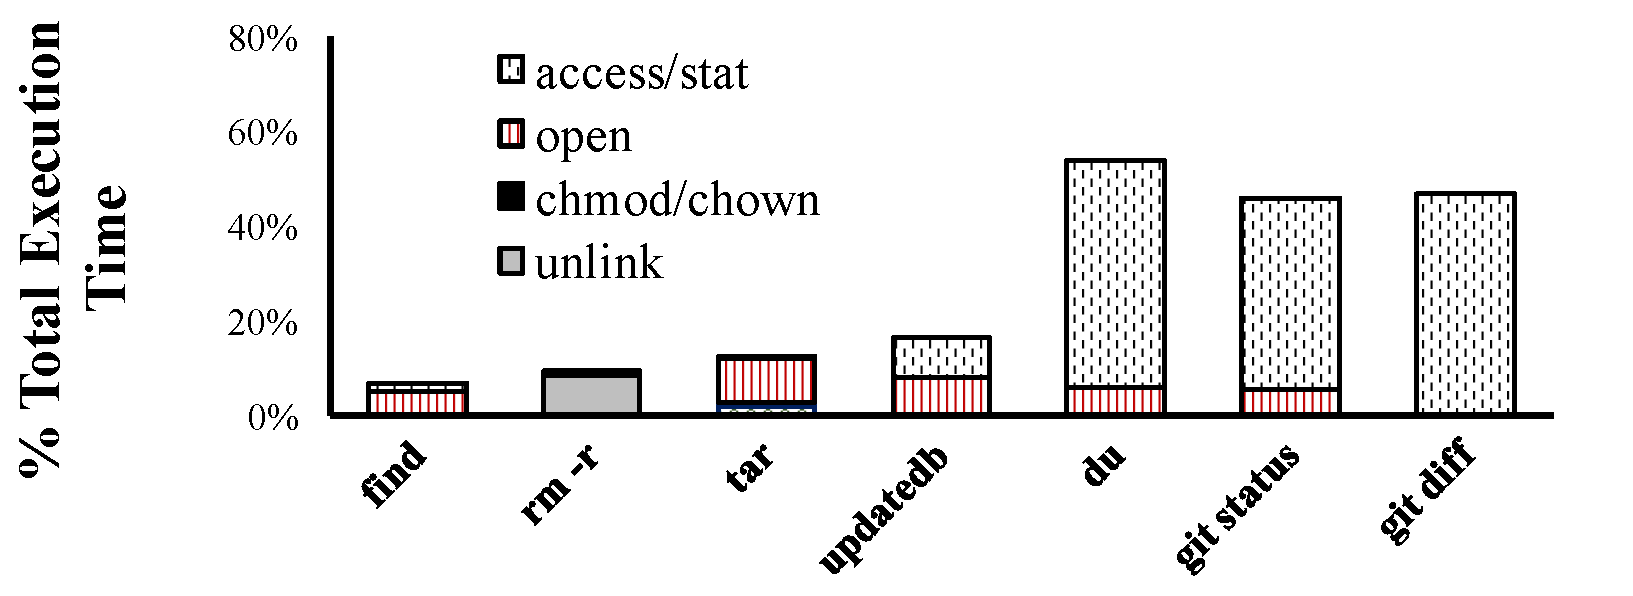
\includegraphics[width=5in]{dcache/plots/syscall-percentage.pdf} \\
\caption[Fraction of execution time on path-based system calls.]
{Fraction of execution time in several common utilities spent
executing path-based system calls with a warm cache, as measured with ftrace.}
\label{fig:dcache:lookup-frac}
%\vspace{-10pt}
\end{figure}

%\fixmedp{Please check these \% against time.  I think git diff is too high.  git status seems ok.}

Directory caches are essential for good application performance.
%Unix was designed such that ``(almost) everything is a file'',
%thus even accesses to in-memory file systems, device files, FIFOs and domain sockets
%first pass through the directory cache.
%In other words, 
Many common system calls must operate on file paths,
which require a directory cache lookup.
For instance, between 10--20\% of all system calls in the iBench system call traces do a path lookup~\citep{filenotafile}. 
Figure~\ref{fig:dcache:lookup-frac} lists the fraction of total execution time
%, as well as system time, 
several common command-line applications spend executing path-based system calls
(more details on these applications and the test machine in \S\ref{sec:dcache:eval}).
We note that these system calls include work other than path lookup,
and that these numbers include some instrumentation overhead;
% are coarse measurements that include  and work than path lookup;
%, and includes some time 
%for synchronous I/O (e.g., during {\tt rename}) as well as non-path tasks (e.g., creating 
%a file handle as part of {\tt open});
nonetheless, in all cases except {\tt rm},
the system call times and counts are dominated by
{\tt stat} and {\tt open}, for which 
%can be serviced from cache and for which 
path lookup is a significant component of execution time.
For these applications, path-based system calls account for 6--54\% of total execution time.
%and 25--77\% of system time.  
This implies that
lowering path lookup latency is
 one of the  biggest 
opportunities for a kernel to improve these applications' execution time.




\begin{figure}[t!]
\centering
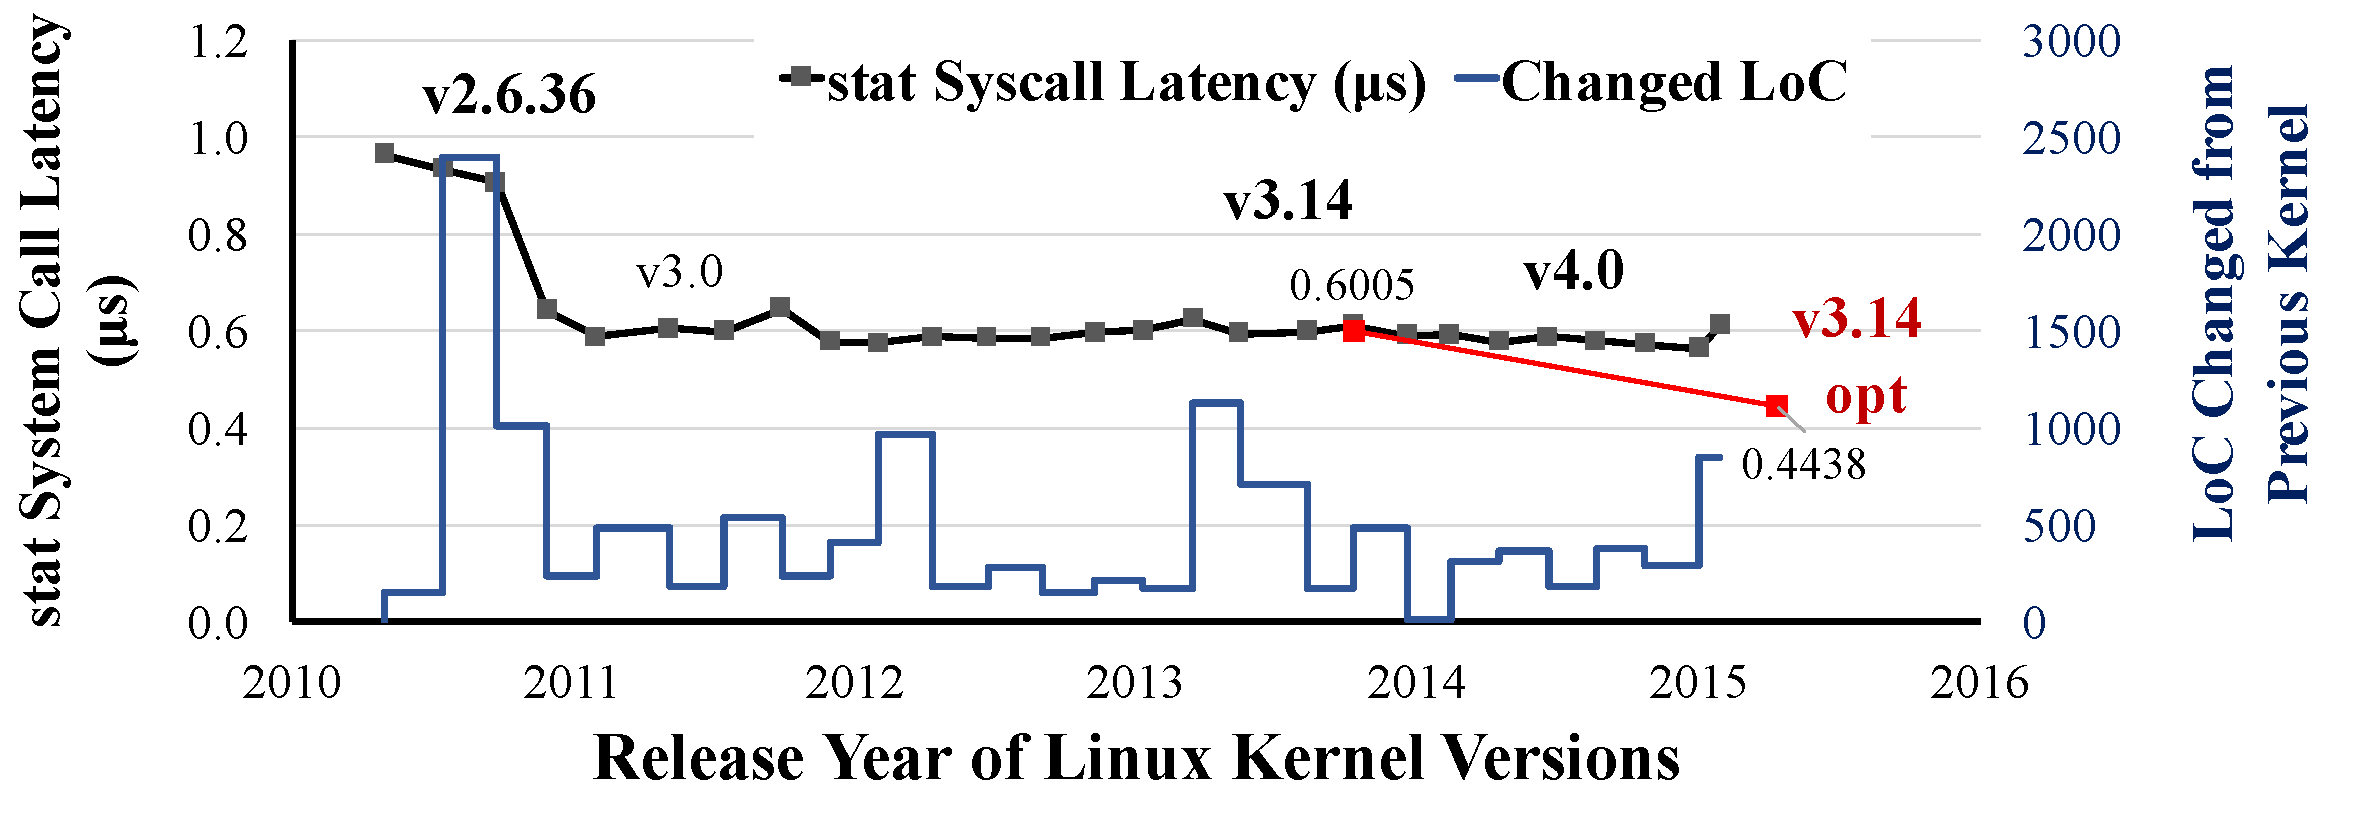
\includegraphics[width=6in]{dcache/plots/latency-by-version.pdf}
\footnotesize
\caption[Lantecy of {\tt stat} system call over years.]
{Latency of {\tt stat} system call with a long path {\tt XXX/YYY/ZZZ/AAA/BBB/CCC/DDD/FFF} on Linux over four years (lower is better), as well as the churn within the directory cache code (all insertions in {\tt dcache.c}, {\tt dcache.h}, {\tt namei.c}, {\tt namei.h} and {\tt namespace.c}). 
%Our optimizations significantly improve performance that has otherwise plateaued, despite significant ongoing developer effort.  
Our optimized \linuxver{} kernel 
further reduces {\tt stat} system call latency by \statspeedup{}\%.}
%\vspace{-15pt}
\label{fig:dcache:by-version}
\end{figure}


%\fixmedp{Add more evidence of lookup importance here: For instance, fraction of lookup time in file-related syscalls, or total lookup time in applications bound on file lookup latency.  }
Unfortunately, even directory cache hits are costly---0.3--1.1 \us{} for a {\tt stat} on our test Linux system, compared to only .04 $\mu$s for a {\tt getppid} and 0.3 \us{} for a 4 KB {\tt pread}. 
%\fixmetsai{Don, check this, I think read will be a better example, getppid is too trivial.}
This issue is taken particularly seriously in the Linux kernel community, which has 
made substantial revisions and increasingly elaborate optimizations to reduce the hit cost
of its directory cache, such as removing locks from the read path or replacing lock ordering with deadlock avoidance in a retry loop~\citep{corbet09jls,dcache-rcu}.
Figure~\ref{fig:dcache:by-version} plots directory cache hit latency against  lines of directory cache code changed 
over several versions of Linux, using a path-to-inode lookup \microbench{} on the test system described
in \S~\ref{sec:dcache:eval}.
These efforts have improved hit latency by 47\% from 2011 to 2013, but have plateaued
for the last three years.
%\fixmedp{if time, filter irrelevant changes from code deltas}
%at the cost of substantial developer effort.
%This latency appears to have plateaued 

The root of the problem is that the POSIX path permission semantics
seemingly require work that is linear in the number of path components,
and severely limit the kernel developer's implementation options.
%The root of this problem is that current directory cache
%designs reflect a straightforward implementation of the POSIX specification,
%which would seemingly require work that is linear in the number of path components.
For instance, in order to open file {\tt /\fnone{}/\fntwo{}/\fnthree{}} 
%for reading, 
one must have search permission
to parent directories {\tt /}, {\tt /\fnone{}}, and {\tt /\fnone{}/\fntwo{}},
as well as permission to access file {\tt \fnthree{}}.
The Linux implementation %of this specification is straightforward, 
simply walks the directory
tree top-down to check permissions.  
Unfortunately, when the critical path is dominated by 
walking a pointer-based data structure, 
including memory barriers on some architectures for multi-core consistency, 
modern CPUs end up stalling on hard-to-prefetch loads.
Moreover, because so many Linux features are built around this behavior, such as Linux Security Modules (LSMs)~\citep{wright+lsm},
namespaces, and mount aliases, it is not clear that any data-structural enhancements
are possible without breaking backward-compatibility with other Linux kernel features.
A priori, it is not obvious that a faster lookup algorithm, such as a single hash table lookup, 
can meet these API specifications and kernel-internal requirements; to our knowledge,
no one has tried previously.

%This paper proposes a decomposition of the directory cache, which allows
%most lookup operations to execute with a single hash table lookup (\S\ref{sec:dcache:dcache}),
%as well as optimizations to reduce the miss rate based on information that is {\em already in the cache}, but not used effectively (\S\ref{sec:dcache:readdir}).
%Our design maintains compatibility (\S\ref{sec:dcache:generalize}) through 
%several essential insights, including 
%how to separate the indexing of paths from checking parent permissions,
%and how to effectively and safely memoize the results of access control checks.


%% This paper proposes several new ways to organize a directory cache, which can yield 
%% substantial performance improvements over the current state of the art.
%% %This paper demonstrates that, despite this developer effort, there is still a substantial 
%% %missed opportunity hiding behind historical, intuitive, but not fundamental design choices.
%% Most of the Linux directory cache design reflects a straightforward implementation of the POSIX 
%% specification. %, with a division of labor that is suitable for mainstream file systems.

%This paper presents an alternative directory cache organization, which 
%improves performance by separating logical tasks, such as separating path indexing from permission checking; yet the design is sufficient to retain compatibility with POSIX.
%In the case of path lookup, 
%this paper demonstrates how 
%a per-component tree walk can be replaced with a single hash table lookup (\S\ref{sec:dcache:dcache}).
% without violating POSIX compliance.

%Our optimizations improve the performance of frequent lookup operations, but 
%introduce several costs, described in \S\ref{sec:dcache:dcache} and measured in \S\ref{sec:dcache:eval},
%which  we believe are acceptable and a net improvement for applications.
%First, these optimizations slow down infrequent modifications to the directory hierarchy, such as {\tt rename}, {\tt chmod},
% and {\tt chown} of a directory. 
%However, these slower operations
%account for less than .01\% of the system calls in the iBench traces~\citep{filenotafile}.
%Second,  the memory overheads of the dcache are increased.
%%(45\% per \dentry{}, as well as some  in our prototype).
%%(\fixmedp{XX MB} in our tests).  
%Third, lookup has a 
%probability of error from signature collisions that can be adjusted to be negligible
%%($2^{-141}$ in our configuration), 
%and within acceptable thresholds widely used by data deduplication systems~\citep{Debnath:2010:CSU:1855840.1855856, Srinivasan:2012:ILI:2208461.2208485, Quinlan:2002:VNA:645371.651321, Zhu:2008:ADB:1364813.1364831}.
%%, as well as how to remove
%%all memory barriers from the lookup path (\S\ref{sec:dcache:update}).
%In the micro-benchmark of Figure~\ref{fig:dcache:by-version}, our directory cache 
%optimizations improve lookup latency by 
%%revisions improve latency of accessing a long path
%%by 
%\statspeedup{}\% over unmodified Linux.
%%Our design addresses other missed
%%opportunities, such as identifying new opportunities to reduce the miss rate
%%through caching directory completeness.
%%\fixmedp{Do we want to highlight LoC?  3K is more than anything in the graph} \fixmetsai{Probably just mention in the evaluation. It's a metric that we should provide, but it's not awfully interesting.}
%%The total lines of code changed are fewer than 3,000 out of \fixmedp{XX}.
%%\fixmedp{Can we get 
%%, yet changes fewer than 3,000 lines of code.

%% SOSP cut - kind of long-winded
\begin{comment}
This paper rethinks current Linux directory cache design choices in light of the following goals:
\begin{compactitem}
\item {\bf Minimize the cost of a cache hit.} (\S\ref{sec:dcache:dcache}).
This means maximizing the benefit of temporal locality for frequent operations,
while pushing extra work of consistency maintenance onto less frequent, already-expensive operations.
%such as handling cache miss or updating massive metadata,
%in order to improve very frequent operations.
\item {\bf Maintain legacy compatibility.} (\S\ref{sec:dcache:generalize}).  Unix path semantics are complex, required by applications, file systems, and security modules, frustrating otherwise straightforward optimizations.  However tempting it may be to redesign path behavior to facilitate caching, path operations must exhibit the same behavior, with lower latency.
\item {\bf Never miss the same request twice in quick succession.} (\S\ref{sec:dcache:readdir}).  A number of less-frequent operations, such as reading a directory or secure temporary file creation, always miss in the cache {\em even if enough information is in cache to satisfy the operation.}  
%Of course, infrequent accesses should still be subject to a cache replacement policy, such as LRU.
\end{compactitem}
%Although directory caches must implement more complex semantics than a hardware memory cache,
%these principles should seem familiar to the reader with a basic architecture background.
%sadly, the Linux directory cache design violates all three.
\end{comment}

%This paper introduces several techniques to improve the performance of a directory cache,
%This paper explains several practical directory cache optimizations,
This paper demonstrates that these techniques improve performance for applications that use the directory cache heavily,
and the harm is minimal to applications that do not benefit.
%and that the worst case \microbench{} is only 12\% slower within \fixmedp{XX}\% of unmodified Linux.
%Each optimization we describe improves performance in isolation, and all can be combined.
%These optimizations change very few lines of code, and are backward-compatible with 
%legacy applications.  
%These changes are encapsulated in the VFS---individual file systems do not have to change their code.
%This paper describes a  prototype of these improvements implemented in Linux \linuxver{}.
%\S~\ref{sec:dcache:background} explains that the directory cache structure of Mac OS X, FreeBSD, and Solaris 
%are sufficiently similar that these principles should generalize.
%we compare and contrast Linux's directory cache
%with Mac OS X, FreeBSD, and Solaris in \S\ref{sec:dcache:background}, and explain inline how each
%optimization could be generalized to these other OS kernels.





%% \item {\bf Modularization and stackability}:
%% Any changes or optimizations must be implemented as modules inside Linux's VFS,
%% and can be stacked on top of the original design or any future optimizations. 
%% \item {\bf Backward compatibility}:
%% Any changes or optimizations must maintain least requirement of modifying any
%% file systems.
%% \item {\bf Generalization to other OSes}: Any changes or optimizations must be portable to other OSes with reasonable effort and change of design.




%% \dcache{} is proven to be effective on improving storage performance.
%% Experiments shows that,
%% in a Linux 3.x kernel, a \dcache{} with a xxx\% hit rate can speed up
%% metadata lookup and fetching time by xxx times.
%% \fixmetsai{experiment result, Linux version, and fs specs here}
%% However, we observed that Linux maintainers have made
%% constant and non-trivial efforts to improve \dcache{} in the Linux kernel.
%% We studied all \dcache{}-related source files in the Linux kernel Git repository,
%% and discovered that maintainers have committed
%% on average xxx revisions per source files.

%% We tested metadata lookup time on primary \dcache{}-related revisions.
%% Most changes on \dcache{} system only create xxx\%-xxx\% speed-up
%% than their predecessor.
%% \fixmetsai{result and graph here}.
%% Moreover, improvement to \dcache{} is still work-in-progress
%% for Linux maintainers.
%% \fixmetsai{reference to threads for latest dcache discussions}. 
%% All the evidences show that,
%% despite of significant reduction of storage operations,
%% efficiency of \dcache{} system internally still remains as a concern.

%% We argue that the design of \dcache{} needs to be carefully re-examined,
%% to fundamentally identify any missed opportunities that
%% improve value of \dcache{}.
%% At a high level, most optimization works for \dcache{} are focused on
%% improving ``how to cache'',
%% but we want to also lay eyes on ``what to cache'',
%% to ensure any valuable information returned from file systems
%% be captured by \dcache{} system.

%The contributions of this paper are as follows:
%\begin{compactitem}
%\item A performance analysis of the costs of path lookup and the opportunities
%to improve cache hit latency.
%\item A directory cache design that improves path lookup latency with a combination of techniques, including:
%  \begin{compactitem}
%  \item Indexing the directory cache by full path, reducing average-case lookup from linear to constant in the number of path components.
%  \item A Prefix Check Cache (PCC) that separates permission checking from path caching.  The PCC memoizes permission checks, and is compatible with LSMs~\citep{wright+lsm}.
%  \item Reducing the cost of checking for hash bucket collisions with path signatures.
%  \end{compactitem}
%\item Identifying opportunities to leverage metadata the kernel already has to reduce miss rates, such as tracking whether a directory is completely in cache.
%\item Carefully addressing numerous, subtle edge cases that would frustrate rote application of these techniques, such as integration with symbolic links and Linux namespaces.
%\item A thorough evaluation of these optimizations.  For instance, our optimizations improve throughput
%of the Dovecot IMAP server by up to \dovecotspeedup\% and latency of 
%updatedb by up to \updatedbspeedup{}\%.
%%git version control system by up to 25\%.
%
%\end{compactitem}

%\section{Background}
\label{sec:background}

This section summarizes \sgx{},
and current design points for running or porting applications on \sgx{}.
%and the legacy frameworks of porting 
%including \haven{}~\cite{baumann14haven}, \scone{}~\cite{osdi16scone}, and Panoply~\cite{shinde17panoply}. 


\subsection{Software Guard Extensions (SGX)}
\label{sec:background:sgx}

%\begin{figure}[t!]
%\centering
%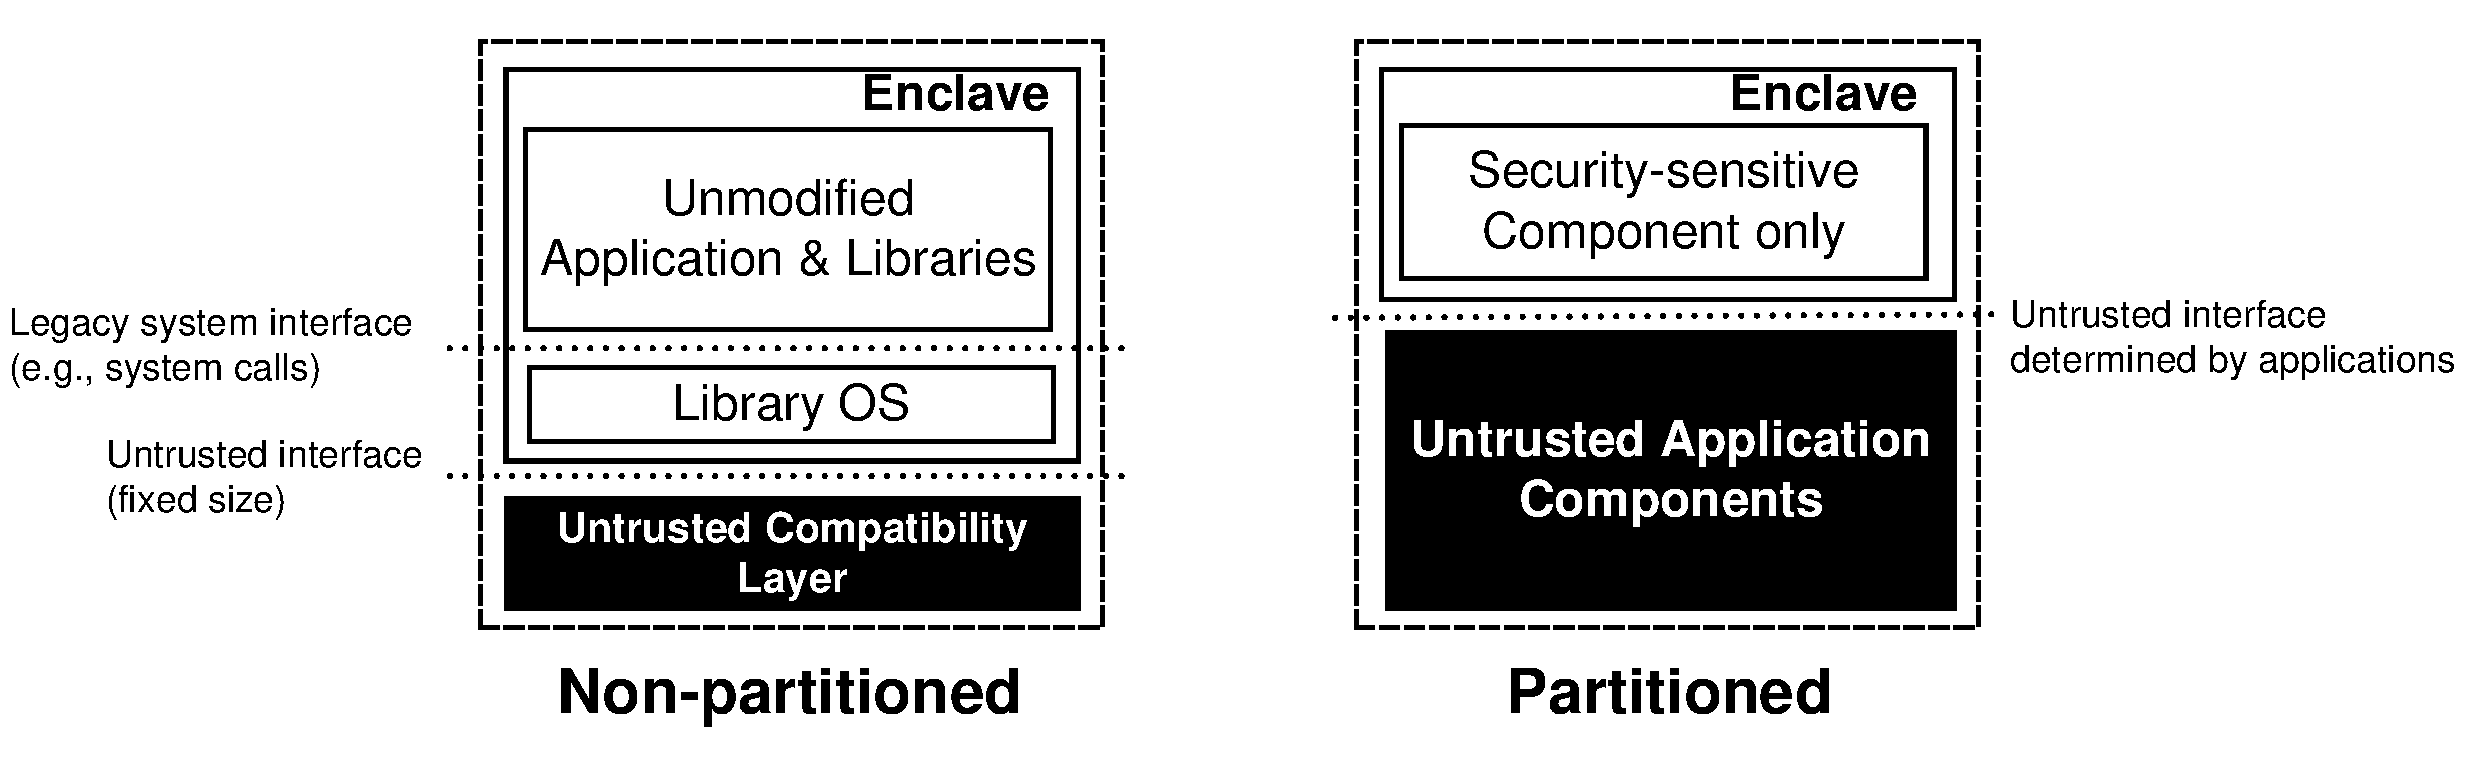
\includegraphics[width=\linewidth]{figures/libosvssdk.pdf}
%\footnotesize
%\vspace{-0.3in}
%\caption{
%Comparison between libOS-based model (e.g., \haven{} and \graphenesgx{})
%and SDK-based (SDK for \sgx{}) model for migrating applications in enclaves.
%Green (light) boxes are trusted components and red (dark) boxes are untrusted.
%The libOS-based model often yields a larger TCB in the enclave,
%while the SDK-based model requires developers to be responsible of
%securing the enclave on the untrusted interface.
%}
%\label{fig:libosvssdk}
%\end{figure}

The primary SGX abstraction is an \emph{enclave}: an isolated execution environment within the virtual address space of a process.
The code and data in enclave memory do not leave the CPU
package unencrypted; when memory contents are read back into cache,
the CPU decrypts the contents, and checks the integrity of cache lines and the virtual-to-physical mapping.
SGX also cryptographically measures the integrity of enclaves at start-up, and 
provide attestation to remote systems or other enclaves.
%Remote entities can identify the owners of enclaves by distinguishing the cryptographic measurements
%generated with different signing keys.

%%% \sgx{} is a new feature on the 6th-genaration \intel{} CPUs.
%%% it contains a set of new x86/64 instructions, to initiate, destroy, and attest isolated execution environments (i.e., enclaves) in the address space of applications.
%%% When \sgx{} loads an application in an enclave,
%%% the code and data of the application will remain encrypted in the main memory,
%%% forbidding any mean to eavesdrop the application secrets.
%is a set of new x86/x64 instructions introduced
%to the latest \intel{} CPUs,
%to bootstrap an isolated execution environment
%inside applications' virtual memory address space.
%\sgx{} creates a memory region
%(generally referred as {\bf enclave}), storing both the code and data of the isolated execution,
%which stays encrypted in DRAMs and only the CPU is capable of encryption and decryption.
%The CPU derives the encryption key
%from the cryptographic measurement of the initial state of enclave memory,
%to allow remote entities to verify the soundness of execution and establish the trust
%needed for provisioning sensitive data.

\sgx{} enables a threat model where one only trusts the \intel{} CPUs and the 
code running in the enclave(s).
%whereas the rest of application, system software, off-CPU-package hardware devices and providers are untrusted. 
\sgx{} protects applications from three different types of attacks on the same host, which are summarized in Figure~\ref{fig:sgx-threats}: untrusted application code inside the same process but outside the enclave; operating systems, hypervisors, and other system software;
%\fixme{added Mona's suggestion}
other applications on the same host; and off-chip hardware.
A SGX enclave can also trust a remote service or enclave, and be trusted after inter-platform attestation~\cite{sgx-attestation}.




%%% \begin{compactenum}

%%% \item {\bf Inside process memory:}
%%% \sgx{} partitions the application process into two privilege levels, as the trusted part (in enclaves) which can access the whole process memory, and the untrusted part (outside enclaves) forbidden to access enclave memory.
%%% %the privileged part (in the  enclave region) can access all process memory,
%%% %while the unprivileged part (outside the enclave region) is limited to access only data that are not isolated by \sgx{}.

%%% \item {\bf From hosting OSes or hypervisors:}
%%% \sgx{} assumes that OSes and hypervisors can be compromised by either exploiting system vulnerabilities
%%% or malicious system software installed by administrators.
%%% Both types of compromise are legitimate threats to modern OSes, due to complexity of modern OSes and usage of public facilities like clouds.

%%% %Operating systems or hypervisors
%%% %that are either compromised by rootkits
%%% %or deliberately modified by the host providers.
%%% %An attacking host can access the raw data in DRAMs, or remap the
%%% %physical pages to other contexts.

%%% \item {\bf Physically from the hardware:}
%%% One type of attacks that cannot be defended by software-based solutions~\cite{flicker, criswell2014virtualghost}
%%% is from the attackers who have physical access to the hosts.
%%% \sgx{} can resist attacks on the host hardware
%%% including hacking peripheral devices like ethernet cards and connectors~\cite{hudson15thunderstrike}, tapping into buses, or eavesdroping DRAM data using Cold-boot attack~\cite{halderman09coldboot}.


%%% \end{compactenum}


%%% \sgx{} protects an application against unpredictable threats from both local and remote hosts.
%%% \sgx{} establishes a trusted path
%%% from one enclave to another,
%%% providing end-to-end protection to both enclaves to
%%% exchange data with confidentiality and integrity.
%%% %, processing the data and returning the computation results with end-to-end protection.
%%% We can further divide up the protection using \sgx{} into three elements:
%The use cases of \sgx{} mostly involve the process that an enclave
%retrieves a signed attestation from the processor,
%to exchange provisioning of critical information from remote servers.
%The purpose of such process is equivalent to
%expanding the trusted execution
%from remote servers
%to untrusted hosts,
%to harness resources such as CPU cycles and DRAMs.

%%% \begin{compactenum}

%%% \item {\bf Isolated execution:}
%%% \sgx{} guarantees the execution initiated in an enclave
%%% to be isolated from any part of the system except the enclave itself.
%%% %any part of the system except the enclave itself can access the execution state. 
%%% Achieved by the secrecy of encryption keys in \intel{} CPUs.

%%% \item {\bf Attestation of integrity:}
%%% Remote entities with a \sgx{}-enabled CPU can verify the integrity of an enclave, using the \intel{} Attestation Services (ISV)~\cite{isv}.
%%% %for its integrity of running the exact code that it is given.
%%% Achieved by the uniqueness of CPU keys to sign the cryptographic measurement of enclaves.

%%% \item {\bf Authentication:}
%%% Remote entities can identify the owners of enclaves by distinguishing the cryptographic measurements generated with different signing keys.


%%% %explicitly launched for processing the specific tasks, regardless of the identicality of execution.
%%% %That is, two mutually distrusting users can launch the same execution in  separate enclaves, yet be able to distinguish by the measurements as MACs (Message Authentication Code) signed by the users' private keys.

%%% \end{compactenum}


%One must note that \sgx{} only promises the integrity of application binaries
%initially loaded in enclaves.
%The gap between integrity of binaries and complete security has to be filled
%by ones who develop and approve the applications.
%More specifically, the clients are responsible of
%testing whether the applications contain any vulnerabilities
%that lead to information leak.
%To minimize the risk of leaving any flaws in the applications unintentionally,
%developers often tend to cut down the trusted computing base (TCB)
%of the applications. With smaller TCB, clients who launched the enclaves
%can more easily reason about the thoroughness of securing the execution.

%To achieve smaller TCB, the software development kit of \sgx{}
%intends to encourage developers to partition the applications and
%keep only security sensitive components in the enclaves.
%Such an intention is exactly contradicted by the trust model of \haven{},
%which must trust the loaded application as a whole.
%Except for the cases in which the whole applications must be secured,
%\haven{} actually downgrades the trustworthiness of enclaves.
%Figure~\ref{fig:libosvssdk} shows the comparison of the two models.


%%% By synthesizing and streamlining these three elements (i.e., isolation, attestation and authentication),
%%% \sgx{} provides a promising build block to securing applications
%%% from unpreditable security threats.

%developing applications
%that are resistant to unpreditable, unavoidable threats.
%Users expect \sgx{} to build up a wall for protecting the sensitive data, even against a catastrophic scenario like a complete takeover of the infrastructure.  

%\fixmedp{Explain how to read the figures in the captions. What do colors and shading mean?}
%
%\fixme{Disabled the whole discussion about SDK. dp: ok with me, but probably drop from figure} 
\begin{comment}
\subsection{The legacy framework (The \sdk{})}

{\bf Intel's \sgx{} SDK} (software development kit) for Linux~\cite{intel-sgx-sdk} is the official framework
for programming \sgx{} execution within Linux applications.
\sdk{} includes the components of two phases:
a {\bf compile-time utility} to generate a valid executable for running inside enclave,
and a {\bf run-time framework} to trigger the hardware-enforced isolated execution.
The two-phased design is based on the assumption that compilation of applications
is controlled by trusted, security experts,
to retain the trustworthiness of isolation model when running on untrusted OSes.


The work flow of \sgx{} programming using \sdk{} is as follows:
\begin{compactenum}
\item At the build-time (on trusted hosts), developers create a self-contained, static executable as the initial code and data after enclave creation.
We refer the executable as an ``enclave image''.
The enclave image is statically links with the enclave infrastructure, which provides enclave APIs (e.g., retrieving attestation) and a extremely small set of POSIX functions (e.g., {\tt memset()}).
After linking, the compile-time utility signs the executable and inserts the enclave signature structure
({\tt SIGSTRUCT}) in the application code.
\item At the execution-time (on untrusted hosts), the enclave image is taken by the framework. The user-space driver then requests enclave creation with the kernel driver, through {\tt ioctl()} to a pseudo-device {\tt /dev/isgx}.
The kernel driver creates and initializes an enclave using the authenticated signature structure,
and a token exchanged from an architectural enclave, {\tt AESMD}, for ensuring the validity of enclave. 
\end{compactenum}





%During the compile time,
%the developers create a self-contained, static binary, as the initial image of an run-time enclave (an ``enclave image'').
%\sdk{} provides the infrastructural libraries (libsgx) for static linking, which contain enclave APIs and few POSIX functions.
%A signing tool of \sdk{} will generates a valid enclave signature
%derived from the enclave image.
%Both the static linking and signing must happen on a trusted, development machine.


%After generating the enclave image, developers then ship it with the rest of application,
%to untrusted hosts (\sgx{}-enabled)
%where the \sdk{} run-time framework is installed.
%The run-time framework provides both kernel and user-space drivers,
%to interface \sgx{} hardware using the new x86 instructions (e.g., {\tt ECREATE}, {\tt EADD}, {\tt EENTER}).
%The framework also includes an architectural enclave (AESM), for validating the enclave attributes (and generating a run-time token),
%and a kernel EPC (enclave page cache) driver that manages paging for all running enclaves.



% includes both compile-time and run-time components:
%for the compile time, the SDK provides all the infrastructure libraries,
%which the applications statically link with,
%and a signing tool that generates the enclave signatures for hardware validation.
%The run-time framework then takes the signed enclave binaries,
%and uses the kernel and user-space drivers to initiate the isolated execution in enclaves.



\sdk{} centers the whole programming model based on the concept of partitioning an application,
and isolating only minimum application code in enclaves.
The partitioning minimizes the risk of compromising the enclaves,
due to smaller trusted computing base (TCB) and less opportunity of omitting security glitches.
With this model,
developers are expected
to identify the part of an application that performs the sensitive operations,
and define an validated interface to
the sensitive part and rest of the application.
\sdk{} encourages partitioning by reducing the difficulty of defining and accessing the interface---a language tool automatically generates the interface code with extra argument-sanitizing code.
The generated interface code essentially filters input and output of the enclave,
and prevents randomly copying memory across the enclave boundary, leaking or corrupting internal data.


%The Intel SDK has its limitations. The infrastructure of the SDK provides APIs in enclaves for accessing SGX features (e.g., attestation), as well as a small set of POSIX APIs
%(\roughly{}10 functions, such as {\tt printf} and {\tt memset}).


Despite that \sdk{} attempts to alleviate the difficulty of partitioning for SGX,
porting a piece of application code that is sophisticated and interactive to the rest of application
is still a significant cost to pay.
In general, developers want to find a reasonable granularity of partitioning---a ``sweet spot'' that partitions the application code neither too small nor too large, 
to nicely balance between frequency of enclave exits and risk of introducing incompatible code.
For an application written in C/C++, partitioning is cumbersome especially if the application is poorly modularized.


Unfortunately, the limited POSIX support in the \sdk{} infrastructure really strikes
the opportunity of fine-grained partitioning.
The lack of POSIX APIs in the infrastructure is fundamental, due to the restriction
on OS interaction from the enclaves.
The missing APIs encapsulates system calls, which can expose the enclave to some risky OS interaction model, such as {\bf Iago Attacks}~\cite{checkoway13iago}.

%In conclusion, this work targets on completing the API support, either at POSIX level or system calls,
%while retaining the isolation model.
%The platform can assist developers to refocus on partitioning applications for minimizing the risks.

\end{comment}

\subsection{SGX Software Design Space}

This subsection summarizes the principal design choices facing any 
framework for running applications on SGX.  We explain the decisions in
recent systems for SGX applications, and the trade-offs in this space.

\begin{figure}[t!]
\centering
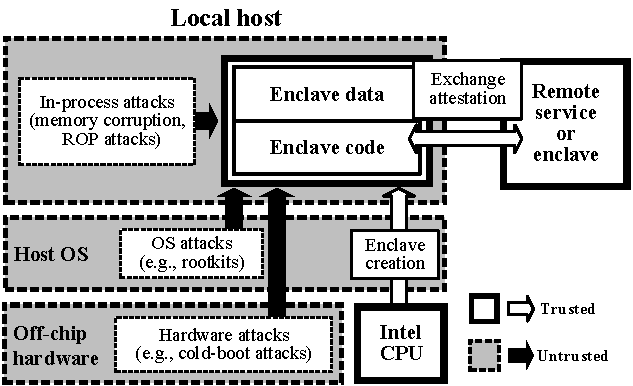
\includegraphics[width=.5\linewidth]{sgx.pdf}
\caption{The threat model of \sgx{}. \sgx{} protects applications
from three types of attacks:
in-process attacks from outside of the enclave,
attacks from OS or hypervisor, and attacks from off-chip hardware.}
% Red (dark) boxes are untrusted components and green (light) boxes are trusted.}
%For each enclave, \sgx{} establishes the chain of trust from the \intel{} CPU.
%Enclaves across physical machines or even infrastructures can remotely attest the integrity of execution, using the signatures generated and signed by the CPU.
%Green (light) boxes and arrows represent the trusted components and operations, and red (dark) boxes and arrows represent the otherwise.
\label{fig:sgx-threats}
\end{figure}

\paragraph{How much functionality to pull into the enclave?}
At one extreme, a library OS like Haven~\cite{baumann14haven} pulls most
of the application-supporting code of the OS into the enclave.
On the other extreme, thin ``shim'' layers, like SCONE~\cite{osdi16scone} and Panoply~\cite{shinde17panoply} 
wrap an API layer such as the system call table.
Pulling more code into the enclave increases the size of the TCB,
but can reduce the size and complexity of the interface, and attack surface, 
between the enclave
and the untrusted OS.

The impact of this choice on performance
largely depends on two issues. First, entering or exiting the enclave 
is expensive; if the division of labor reduces enclave border crossings, 
it will improve performance.
The second is the size of the Enclave Page Cache (EPC),
limited to 128MB on version 1 of SGX.
If a large supporting framework tips the application's working set size
past this mark, the enclave will incur expensive swapping.


\paragraph{Shielding complexity.}
SGX hardware can isolate an application from an untrusted OS, but 
SGX alone can't protect an application that  requires
functionality from the OS.  {\em Iago attacks}~\cite{checkoway13iago}
are semantic attacks from the untrusted OS against the application, where an unchecked system call return 
value or effect compromises the application.
Iago attacks can be subtle and hard to comprehensively detect, at least with the current
POSIX or Linux system call table interfaces.

Thus, any SGX framework must provide some {\em shielding} support, to 
validate or reject inputs from the untrusted OS.  
The complexity of shielding is directly related to the interface complexity:
inasmuch as a library OS or shim can reduce the size or complexity of the 
enclave API, 
the risks of a successful Iago attack are reduced.

\paragraph{Application code complexity.}
Common example applications for SGX in the literature 
amount to a simple network service running a TLS
library in the enclave, putting minimal demands on a shim layer. 
Even modestly complex applications, such as the R runtime and a simple
analytics package, require dozens of system calls providing wide-ranging functionality, 
including \syscall{fork} and \syscall{execve}.
For these applications, the options for the user or developer become: 
(1) modifying the application to require less of the runtime; (2) opening and shielding more 
interfaces to the untrusted OS; (3) pulling more functionality into a shim or a library OS.
The goal of this paper is to provide an efficient baseline, based on (3),
so that users can quickly run applications on SGX, and developers can 
explore (1) or (2) at their leisure.

\paragraph{Application partitioning.} An application can have multiple
enclaves, or put less important functionality outside of the enclave.
For instance, a web server can keep cryptographic keys in an enclave,
but still allow client requests to be serviced outside of the enclave.
Similarly, a privilege-separated or multi-principal application might create a separate enclave for
each privilege level.

This level of analysis is application-specific, and beyond the focus of this paper.
%which is on running unmodified applications in enclaves.
However, partitioning a complex application into multiple enclaves
can be good for security. In support of this goal,
\graphenesgx{} can run smaller pieces of code, such as a library, in an enclave, as well as
coordinate shared state across enclaves.

%* Partitioned vs. unpartitioned app?

%** Right choice depends a lot on whether the app has multiple principals or security concerns.

\begin{comment}
\fixmedp{Did a first cut at 2.2; needs to integrate the figure (or drop it).  I didn't know what to write for 2.3 yet.  I left the old text below for now (if there is anything you really want to save), but it needs to go away}

\subsection{Open Challenges}

\fixmedp{Here, I would give a taste of some of the issues we solve and why they are hard, like dynamic loading (and maybe fork or IPC).  Keep it short, a few paragraphs.}
\end{comment}

%\begin{figure}[t!]
%\centering
%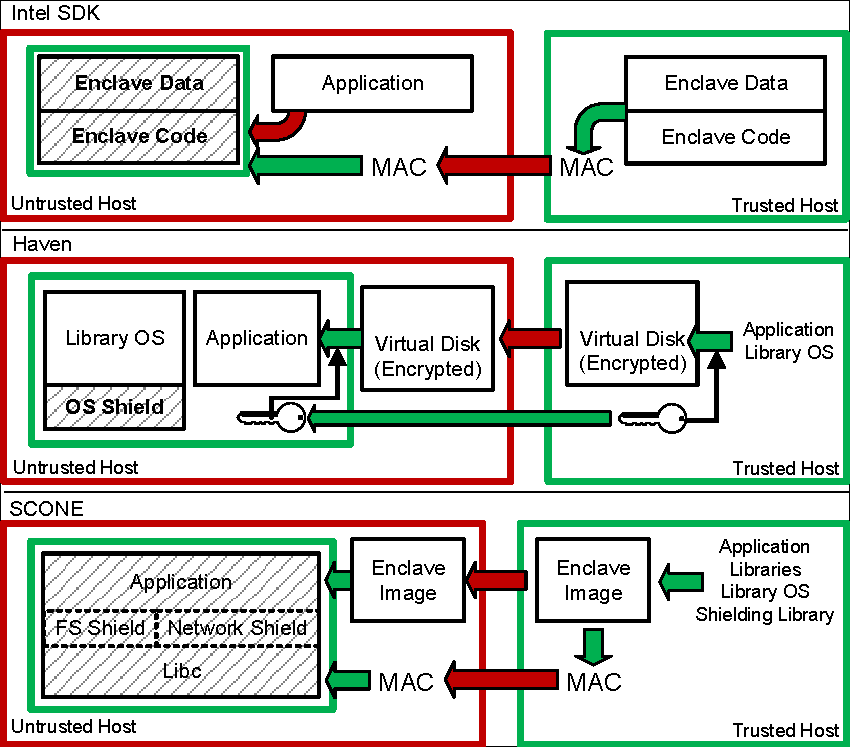
\includegraphics[width=\linewidth]{figures/sdkvslibos.pdf}
%\caption{Comparison of the code integrity model among different \sgx{} frameworks, including the \sdk{}, \haven{} and \scone{}.}
%%Green (light) boxes and arrows represent the trusted components
%%and operations, and red (dark) boxes and arrows represent the otherwise.
%%Patterned blocks represent the code and data included in the initial measurements of the enclaves.}
%\label{fig:sdkvslibos}
%\end{figure}


\begin{comment}
\subsection{\sgx{} shielding systems}
\label{sec:background:shielding-systems}




The current \sgx{} shielding systems, such as \haven{}~\cite{baumann14haven}, \scone{}~\cite{osdi16scone}, and Panoply~\cite{shinde17panoply}, enforce end-to-end isolation to
legacy applications without partitioning.
A \sgx{} shielding system preserves the trusted computing base (TCB)
of an application, and further increases it with a shielding layer to defend against the untrusted OSes.
By avoiding application partitioning,
%model of quarantining an unmodified, COTS application in an \sgx{} enclave.
a shielding system minimizes the effort of reprogramming the applications for \sgx{} execution, often with recompilation or packaging the binaries in an encrypted enclave.
%to merely recompiling or packaging the application code before signing it off for enclave execution.
%These \libos{}es internalize OS features into the enclave, to maintain a fixed-size,
%narrow interface to the untrusted host OSes.
%Porting applications using a \sgx{} \libos{} is vastly different from the programming model of \sdk{}---no programming effort is needed when porting with a \sgx{} \libos{}, and applications are isolated without partitioning.
In the following paragraphs, we compare the current shielding systems with the \graphenesgx{} approach.

\haven{}~\cite{baumann14haven} uses a \libos{} called \drawbridge{} in each enclave
to shield a single-process \emph{Windows} application from the untrusted host OS.
\haven{} absorbs the implementation of system APIs (i.e., Win32 APIs) from the host OS,
%\haven{} uses \drawbridge{}~\cite{porter11drawbridge} as the backbone of its enclave infrastructure, 
and exports a narrow enclave interface on which untrusted inputs are carefully filtered to defend against the Iago-type attacks.
Adding a \libos{} to each enclave causes a bloat of TCB---for \haven{}, the size of a \libos{} binary and shielding layer is \roughly{}200MB.
\haven{} has to establish the trust and integrity in all these binaries loaded into an enclave. Except that the shielding layer is a part of the enclave since its creation, \haven{} enforces the integrity of both the \libos{} and the isolated application,
by storing all binaries on an encrypted virtual disk and relying a remote, trusted server to provision the key for decryption.
\haven{} builds a trusted path from a remote server to local cloud machines,
to securely bootstrap application execution inside the enclaves.
%Other minor comparison between \haven{} and this work: the development and evaluation of \haven{}, at publication, is based on a simulated architecture.
%On the contrast, \graphenesgx{} is a released open-source platform, tested by many developers from institutes and corporations. \fixme{maybe bring up TCB?}



\scone{}~\cite{osdi16scone} isolates Linux micro-services in enclaves as a container-like environment.
After a brief attempt of building a \libos{} like \haven{},
\scone{} chooses a different approach of shielding the system API usage in applications, by designing shielding strategies based on each API.
\scone{} stacks the application on top of file-system and network shielding libraries, and extends a standard library C (musl~\cite{musl}) to securely exit the enclave for system calls.
Within the \sgx{}-aware Libc, \scone{} carefully filters the inputs from the host system calls, as the defend against known Iago attacks.
For instance, \scone{} ensures that pointers given to and returned by a host system call will point to addresses outside the enclave,
to prevent the host OS to manipulate pointers and cause memory corruption in the enclave.
\scone{} also authenticates or encrypts file or network streams
based on configurations given by the developers.


%The \libos{} implementation in \scone{} is based on musl~\cite{musl} and LKL (Linux kernel library)~\cite{lkl}.
%The design of a SCONE enclave (or Secure Container) has similarity
%with a basic block of \graphenesgx{}:
%they both validate input files based on cryptographic methods, and are fully configurable at a per-file basis.
%However, \graphenesgx{} supports a more complete set of Linux system APIs.
%The APIs that \graphenesgx{} especially contributes over \scone{} are the Linux multi-process APIs, including copy-on-write {\tt fork()}, {\tt exec()}, signals, and system V IPC (message queues and semaphores).

Panoply~\cite{shinde17panoply} further reduces the TCB of a shielding system over the SCONE approach, by excluding both a \libos{} and \libc{} from enclaves.
Instead, Panoply uses a shim layer shielding a portion of the POSIX API. The shim layer yields about 20 KLoC as its TCB (trusted computing base), which is much smaller than libc and/or a library OS.
% in other shielding systems.
As Panoply delegates the libc functions outside the enclave, its shim library defends the supported POSIX API,
including 91 {\em safe} functions and 163 {\em wild (unsafe)} functions.
Panoply also supports multi-process API including \fork{}, \exec{}, signaling, and sharing untrusted memory with inline encryption.
Compared to \graphenesgx{}, Panoply has made some different design decisions in supporting multi-process API,
including supporting fork by copying memory on-demand with statically determining memory access,
and using secured messaging for inter-process negotiating instead of coordinating over an encrypted RPC stream.




\subsection{Comparison and security implications}

\fixme{need to drop the SDK discussion, revisit the security claims, and discuss Iago attacks in details.}

Figure~\ref{fig:sdkvslibos} shows the comparison between \haven{}, \scone{}, Panoply, and \graphenesgx{}.
%The \sdk{} model uses a static MAC of the enclave code and data, given to the \sgx{} driver for bootstrapping the isolated execution.
The \haven{} model only initiates enclaves with the OS shield layer,
which unpacks the enclave binaries from a virtual disk---decrypted using a provisioned key.  
The \scone{} model extends the \sdk{} model---it statically links the application binaries with the shielding library, creating a static enclave image verifiable by its MAC. The \sdk{} and \scone{} model retain more flexibility in deploying and integrating \sgx{} enclaves by focusing on the code integrity rather than encryption.

The key concerns that affects users choosing among these solutions are {\bf trusted computing base (TCB) size} and {\bf attack surface}.
However, since all these solutions are based on different design decisions, assumption and requirements, the comparison of TCB size and attack surface is often imprecise and inconclusive.

\paragraph{TCB size.}
Most studies measure the TCB size of a system by the total LoC (lines of code) written for all the trusted components, or the size (in bytes) of all the trusted binaries.
The comparison of TCB size is only meaningful when two systems have comparable system features,
and are order-of-magnitude different in term of LoC or binary size.
For instance, the comparison of TCB size between \haven{} and \scone{} is never an apples-to-apples comparison.
The implemented system features and personalities
in these two systems are fundamentally different, and \haven{} supports a much larger fraction of Windows features than the fraction of Linux features supported by \scone{}.

We argue that the only occasion that the reduction of TCB size
can be convincingly demonstrated is when a design has partitioned a system into isolated components,
or removed unreachable execution paths.
For instance, the \sdk{} promotes application partitioning for \sgx{};
it requires additional partitioning effort but is effective for confining the TCB size.
By statically linking the application binaries
with the shielding layers and standard C library, \scone{} offers more opportunities in stripping the Libc and shield code of unused APIs, and thus reducing its TCB size.



\paragraph{Attack surface.}

Most studies estimate the severity of having an attack surface by the size of interface to the trusted and untrusted components.
The experience of \scone{} provides an important insight for estimating attack surface: the narrowness of interface is not proportional to the difficulty of defending against incoming attacks.
An interface overloaded with too many features or semantics can become a major source of vulnerabilities.

%\subsection{The \graphene{} Library OS}
%
%\graphene{}~\cite{tsai14graphene} introduces a \libos{} design that supports
%both single-process and multi-process Linux applications,
%but retains a narrow host interface (43 functions) as a vantage point for enforcing security isolation.
%The main contribution of \graphene{} is an distributed implementation of the POSIX namespace coordination,
%to support Linux multi-process abstractions across \libos{} instances.
%All the multi-process abstractions in \graphene{} is implemented using simple pipe-like RPC streams,
%without relying on any host memory sharing support.
%Based on this design, \graphene{} can easily isolate mutually untrusting applications,
%by blocking the RPC streams between unrelated applications.
%
%
%
%The design decisions made by \graphene{} are important keys to the \graphenesgx{} framework.
%First, the host interface contains mostly internal abstractions, and three external ones including files, network connections, and RPC streams.
%The simplicity of the host interface facilitates shielding the \libos{}
%from risky OS interaction.
%Moreover, \graphene{} implements multi-process abstractions across instances without memory sharing.
%\graphenesgx{} can rely on the distributed POSIX implementation
%to support multi-process applications across multiple enclaves, by coordination over validated RPC streams.


\end{comment}




\chapter{System Overview}
\label{chap:overview}

\makeatletter
\def\input@path{{overview/}}
\makeatother
\graphicspath{{overview/figures/}}

%\section{Introduction}
%\label{sec:dcache:introduction}

Operating System kernels commonly cache file system data and metadata in 
a virtual file system (VFS) layer, which abstracts low-level file systems into a common API, 
such as POSIX.  
This caching layer has become a ubiquitous optimization
to hide access latency for 
persistent storage technologies, such as a local disk.
%whether a local disk or a network appliance, 
%have substantially higher access latencies than RAM,
%this caching layer 
%% SOSP Space - kind of quacking on
%% Caching
%% the file system directory hierarchy is particularly important because 
%% low-level file systems often spread this information across 
%% multiple disk sectors.
%% If an application wanted to open a single file on a system without a directory cache, 
%% most low-level file systems would issue numerous disk reads to locate the file and check the permissions
%% on the file and its parent directories;
%% a directory cache can commonly avoid these reads.
The directory cache is not exclusively a performance optimization; it also simplifies 
the implementation of {\tt mount}-ing multiple file systems, 
consistent file handle behavior,
and advanced security 
models, such as SELinux~\citep{selinux}.



%\fixmedp{Be charitable to developers, make our strong claims positively (we are really smarties) rather than calling them dummies}


%% Many observation shows that, in most systems, operations to storage are often
%% dominated by hierarchical structure traversal,
%% and fetching metadata of objects.\fixmetsai{references here}~\citep{duchamp94nfs}
%% In many file systems, traversal and metadata fetching
%% create random access patterns,
%% which are slower than sequential access patterns
%% on many storage media, e.g. magnetic disks.

% dp: I think this is getting down in the weeds.  We need to make the case for the work 
%     more strongly and generally first
%% Directory entry cache, a.k.a \dcache{},
%% is an important optimization in Linux kernels
%% to reduce storage operations for traversal and metadata fetching.
%% The design of \dcache{} is comparable to \vnode{} in BSD and \dnlc{} in Solaris.
%% \dcache{}, as well as \vnode{} and \dnlc{},
%% can be explained as a file system layer that
%% responds to requests on a cache hit,
%% but passes requests down to lower-leveled file systems on a cache miss~\citep{zadok06, skinner93}.

%\fixmedp{F1: Maybe thread together an argument about why no one would have tried a one-hop lookup before?}


%\marginpar{\scriptsize \textcolor{blue}{ Michael, I think the high-order bits are mostly right on Fig~\ref{fig:dcache:lookup-frac},
%but these number may change a bit as we refine the measurement}}

\begin{figure}[t]
\scriptsize
\centering
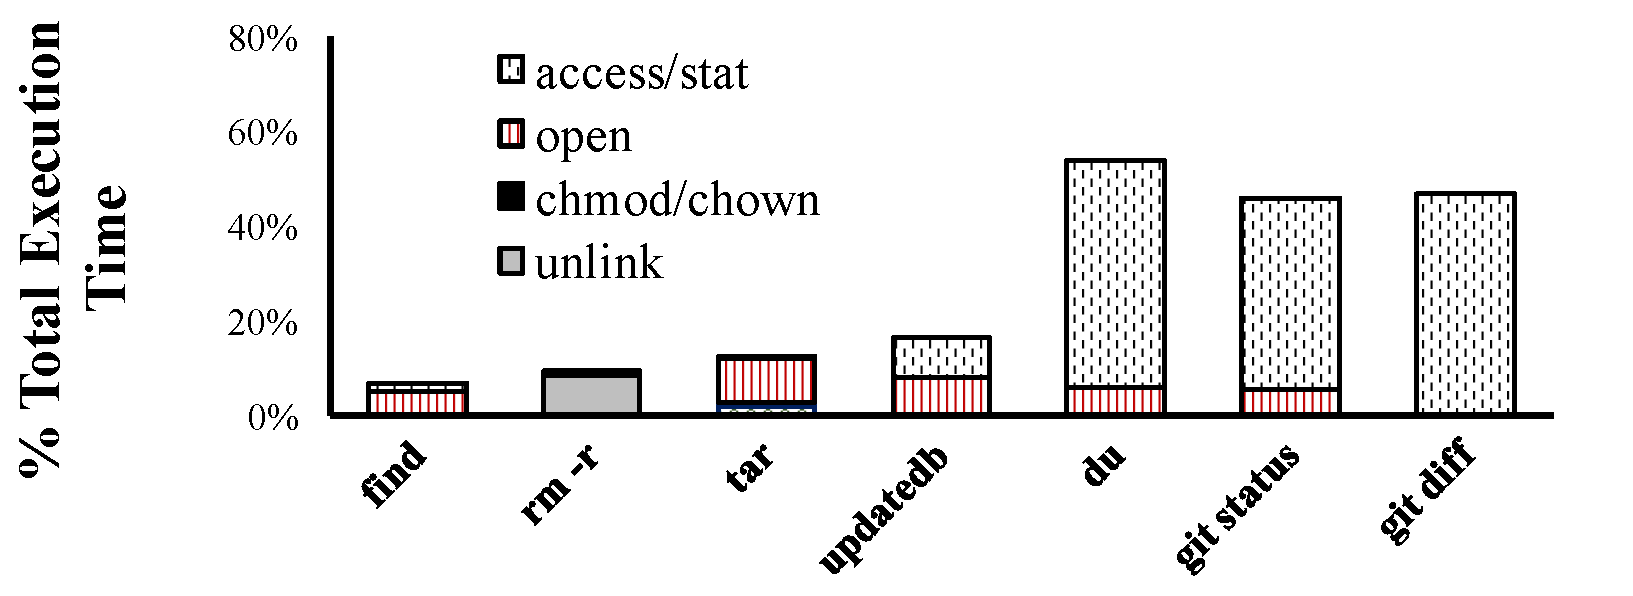
\includegraphics[width=5in]{dcache/plots/syscall-percentage.pdf} \\
\caption[Fraction of execution time on path-based system calls.]
{Fraction of execution time in several common utilities spent
executing path-based system calls with a warm cache, as measured with ftrace.}
\label{fig:dcache:lookup-frac}
%\vspace{-10pt}
\end{figure}

%\fixmedp{Please check these \% against time.  I think git diff is too high.  git status seems ok.}

Directory caches are essential for good application performance.
%Unix was designed such that ``(almost) everything is a file'',
%thus even accesses to in-memory file systems, device files, FIFOs and domain sockets
%first pass through the directory cache.
%In other words, 
Many common system calls must operate on file paths,
which require a directory cache lookup.
For instance, between 10--20\% of all system calls in the iBench system call traces do a path lookup~\citep{filenotafile}. 
Figure~\ref{fig:dcache:lookup-frac} lists the fraction of total execution time
%, as well as system time, 
several common command-line applications spend executing path-based system calls
(more details on these applications and the test machine in \S\ref{sec:dcache:eval}).
We note that these system calls include work other than path lookup,
and that these numbers include some instrumentation overhead;
% are coarse measurements that include  and work than path lookup;
%, and includes some time 
%for synchronous I/O (e.g., during {\tt rename}) as well as non-path tasks (e.g., creating 
%a file handle as part of {\tt open});
nonetheless, in all cases except {\tt rm},
the system call times and counts are dominated by
{\tt stat} and {\tt open}, for which 
%can be serviced from cache and for which 
path lookup is a significant component of execution time.
For these applications, path-based system calls account for 6--54\% of total execution time.
%and 25--77\% of system time.  
This implies that
lowering path lookup latency is
 one of the  biggest 
opportunities for a kernel to improve these applications' execution time.




\begin{figure}[t!]
\centering
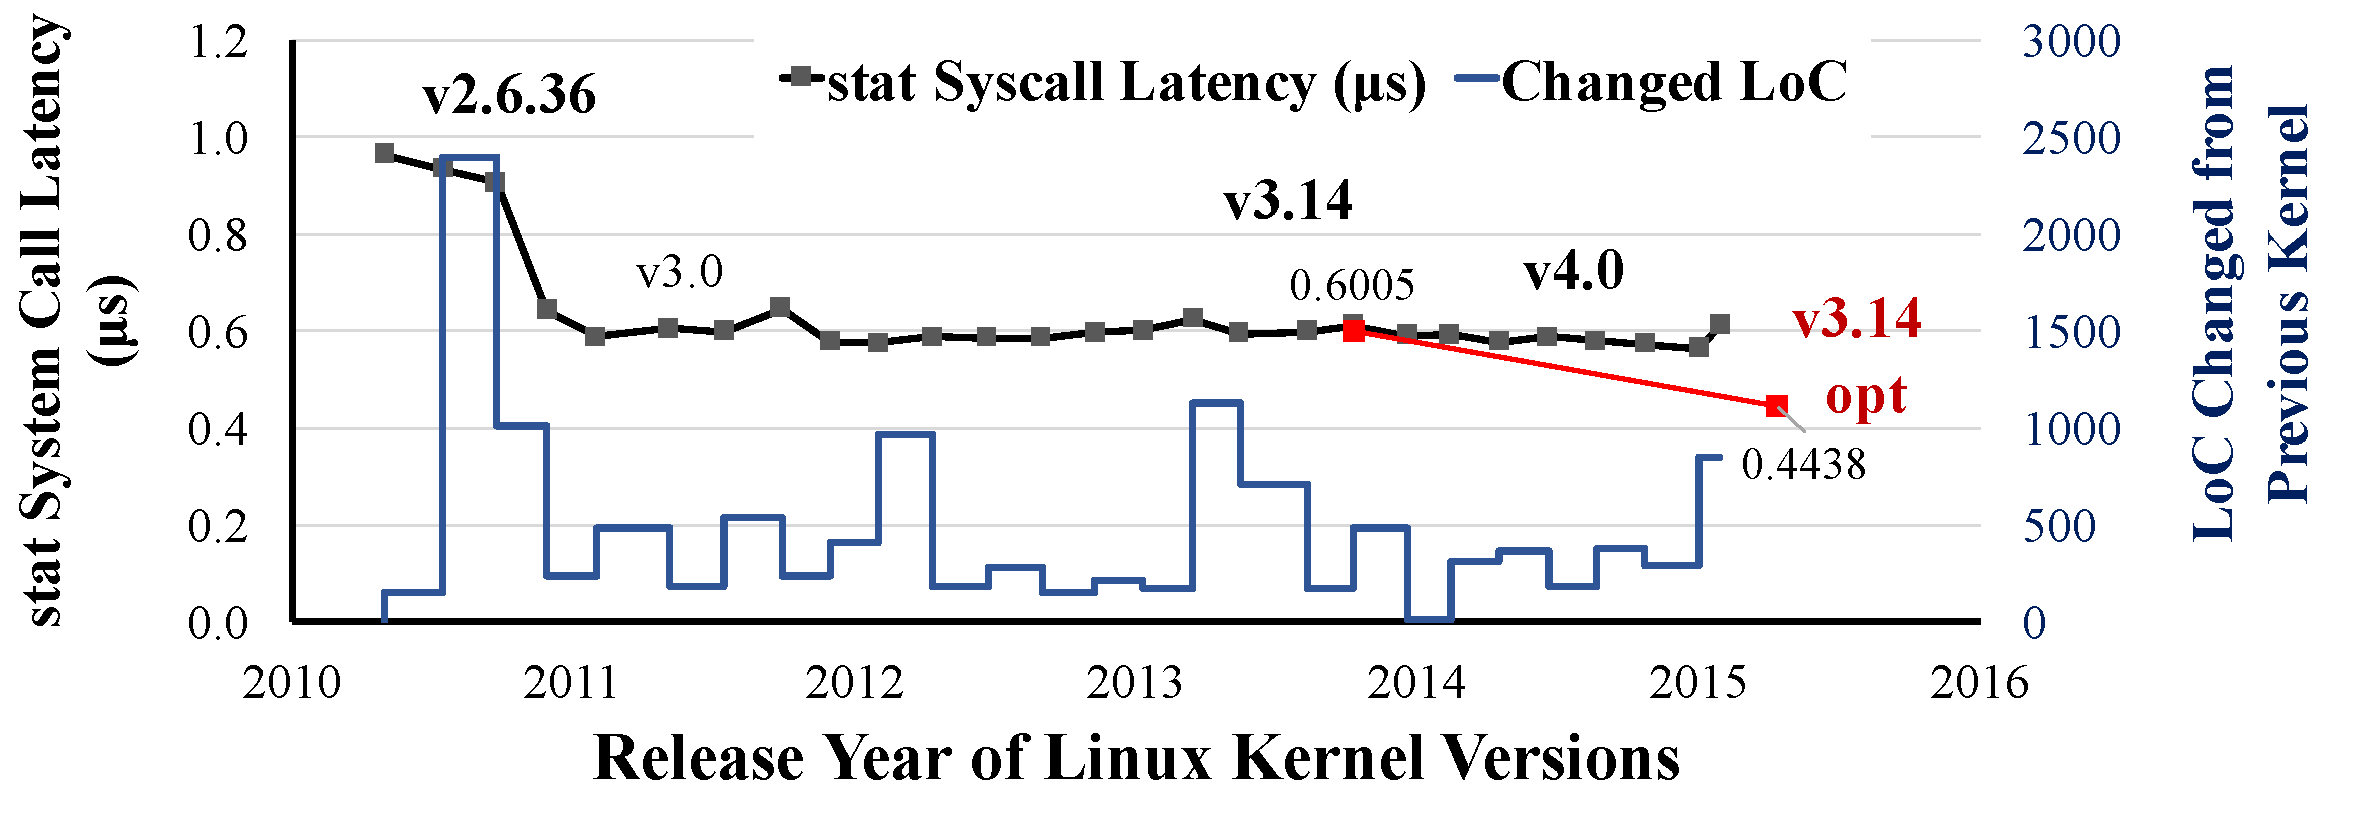
\includegraphics[width=6in]{dcache/plots/latency-by-version.pdf}
\footnotesize
\caption[Lantecy of {\tt stat} system call over years.]
{Latency of {\tt stat} system call with a long path {\tt XXX/YYY/ZZZ/AAA/BBB/CCC/DDD/FFF} on Linux over four years (lower is better), as well as the churn within the directory cache code (all insertions in {\tt dcache.c}, {\tt dcache.h}, {\tt namei.c}, {\tt namei.h} and {\tt namespace.c}). 
%Our optimizations significantly improve performance that has otherwise plateaued, despite significant ongoing developer effort.  
Our optimized \linuxver{} kernel 
further reduces {\tt stat} system call latency by \statspeedup{}\%.}
%\vspace{-15pt}
\label{fig:dcache:by-version}
\end{figure}


%\fixmedp{Add more evidence of lookup importance here: For instance, fraction of lookup time in file-related syscalls, or total lookup time in applications bound on file lookup latency.  }
Unfortunately, even directory cache hits are costly---0.3--1.1 \us{} for a {\tt stat} on our test Linux system, compared to only .04 $\mu$s for a {\tt getppid} and 0.3 \us{} for a 4 KB {\tt pread}. 
%\fixmetsai{Don, check this, I think read will be a better example, getppid is too trivial.}
This issue is taken particularly seriously in the Linux kernel community, which has 
made substantial revisions and increasingly elaborate optimizations to reduce the hit cost
of its directory cache, such as removing locks from the read path or replacing lock ordering with deadlock avoidance in a retry loop~\citep{corbet09jls,dcache-rcu}.
Figure~\ref{fig:dcache:by-version} plots directory cache hit latency against  lines of directory cache code changed 
over several versions of Linux, using a path-to-inode lookup \microbench{} on the test system described
in \S~\ref{sec:dcache:eval}.
These efforts have improved hit latency by 47\% from 2011 to 2013, but have plateaued
for the last three years.
%\fixmedp{if time, filter irrelevant changes from code deltas}
%at the cost of substantial developer effort.
%This latency appears to have plateaued 

The root of the problem is that the POSIX path permission semantics
seemingly require work that is linear in the number of path components,
and severely limit the kernel developer's implementation options.
%The root of this problem is that current directory cache
%designs reflect a straightforward implementation of the POSIX specification,
%which would seemingly require work that is linear in the number of path components.
For instance, in order to open file {\tt /\fnone{}/\fntwo{}/\fnthree{}} 
%for reading, 
one must have search permission
to parent directories {\tt /}, {\tt /\fnone{}}, and {\tt /\fnone{}/\fntwo{}},
as well as permission to access file {\tt \fnthree{}}.
The Linux implementation %of this specification is straightforward, 
simply walks the directory
tree top-down to check permissions.  
Unfortunately, when the critical path is dominated by 
walking a pointer-based data structure, 
including memory barriers on some architectures for multi-core consistency, 
modern CPUs end up stalling on hard-to-prefetch loads.
Moreover, because so many Linux features are built around this behavior, such as Linux Security Modules (LSMs)~\citep{wright+lsm},
namespaces, and mount aliases, it is not clear that any data-structural enhancements
are possible without breaking backward-compatibility with other Linux kernel features.
A priori, it is not obvious that a faster lookup algorithm, such as a single hash table lookup, 
can meet these API specifications and kernel-internal requirements; to our knowledge,
no one has tried previously.

%This paper proposes a decomposition of the directory cache, which allows
%most lookup operations to execute with a single hash table lookup (\S\ref{sec:dcache:dcache}),
%as well as optimizations to reduce the miss rate based on information that is {\em already in the cache}, but not used effectively (\S\ref{sec:dcache:readdir}).
%Our design maintains compatibility (\S\ref{sec:dcache:generalize}) through 
%several essential insights, including 
%how to separate the indexing of paths from checking parent permissions,
%and how to effectively and safely memoize the results of access control checks.


%% This paper proposes several new ways to organize a directory cache, which can yield 
%% substantial performance improvements over the current state of the art.
%% %This paper demonstrates that, despite this developer effort, there is still a substantial 
%% %missed opportunity hiding behind historical, intuitive, but not fundamental design choices.
%% Most of the Linux directory cache design reflects a straightforward implementation of the POSIX 
%% specification. %, with a division of labor that is suitable for mainstream file systems.

%This paper presents an alternative directory cache organization, which 
%improves performance by separating logical tasks, such as separating path indexing from permission checking; yet the design is sufficient to retain compatibility with POSIX.
%In the case of path lookup, 
%this paper demonstrates how 
%a per-component tree walk can be replaced with a single hash table lookup (\S\ref{sec:dcache:dcache}).
% without violating POSIX compliance.

%Our optimizations improve the performance of frequent lookup operations, but 
%introduce several costs, described in \S\ref{sec:dcache:dcache} and measured in \S\ref{sec:dcache:eval},
%which  we believe are acceptable and a net improvement for applications.
%First, these optimizations slow down infrequent modifications to the directory hierarchy, such as {\tt rename}, {\tt chmod},
% and {\tt chown} of a directory. 
%However, these slower operations
%account for less than .01\% of the system calls in the iBench traces~\citep{filenotafile}.
%Second,  the memory overheads of the dcache are increased.
%%(45\% per \dentry{}, as well as some  in our prototype).
%%(\fixmedp{XX MB} in our tests).  
%Third, lookup has a 
%probability of error from signature collisions that can be adjusted to be negligible
%%($2^{-141}$ in our configuration), 
%and within acceptable thresholds widely used by data deduplication systems~\citep{Debnath:2010:CSU:1855840.1855856, Srinivasan:2012:ILI:2208461.2208485, Quinlan:2002:VNA:645371.651321, Zhu:2008:ADB:1364813.1364831}.
%%, as well as how to remove
%%all memory barriers from the lookup path (\S\ref{sec:dcache:update}).
%In the micro-benchmark of Figure~\ref{fig:dcache:by-version}, our directory cache 
%optimizations improve lookup latency by 
%%revisions improve latency of accessing a long path
%%by 
%\statspeedup{}\% over unmodified Linux.
%%Our design addresses other missed
%%opportunities, such as identifying new opportunities to reduce the miss rate
%%through caching directory completeness.
%%\fixmedp{Do we want to highlight LoC?  3K is more than anything in the graph} \fixmetsai{Probably just mention in the evaluation. It's a metric that we should provide, but it's not awfully interesting.}
%%The total lines of code changed are fewer than 3,000 out of \fixmedp{XX}.
%%\fixmedp{Can we get 
%%, yet changes fewer than 3,000 lines of code.

%% SOSP cut - kind of long-winded
\begin{comment}
This paper rethinks current Linux directory cache design choices in light of the following goals:
\begin{compactitem}
\item {\bf Minimize the cost of a cache hit.} (\S\ref{sec:dcache:dcache}).
This means maximizing the benefit of temporal locality for frequent operations,
while pushing extra work of consistency maintenance onto less frequent, already-expensive operations.
%such as handling cache miss or updating massive metadata,
%in order to improve very frequent operations.
\item {\bf Maintain legacy compatibility.} (\S\ref{sec:dcache:generalize}).  Unix path semantics are complex, required by applications, file systems, and security modules, frustrating otherwise straightforward optimizations.  However tempting it may be to redesign path behavior to facilitate caching, path operations must exhibit the same behavior, with lower latency.
\item {\bf Never miss the same request twice in quick succession.} (\S\ref{sec:dcache:readdir}).  A number of less-frequent operations, such as reading a directory or secure temporary file creation, always miss in the cache {\em even if enough information is in cache to satisfy the operation.}  
%Of course, infrequent accesses should still be subject to a cache replacement policy, such as LRU.
\end{compactitem}
%Although directory caches must implement more complex semantics than a hardware memory cache,
%these principles should seem familiar to the reader with a basic architecture background.
%sadly, the Linux directory cache design violates all three.
\end{comment}

%This paper introduces several techniques to improve the performance of a directory cache,
%This paper explains several practical directory cache optimizations,
This paper demonstrates that these techniques improve performance for applications that use the directory cache heavily,
and the harm is minimal to applications that do not benefit.
%and that the worst case \microbench{} is only 12\% slower within \fixmedp{XX}\% of unmodified Linux.
%Each optimization we describe improves performance in isolation, and all can be combined.
%These optimizations change very few lines of code, and are backward-compatible with 
%legacy applications.  
%These changes are encapsulated in the VFS---individual file systems do not have to change their code.
%This paper describes a  prototype of these improvements implemented in Linux \linuxver{}.
%\S~\ref{sec:dcache:background} explains that the directory cache structure of Mac OS X, FreeBSD, and Solaris 
%are sufficiently similar that these principles should generalize.
%we compare and contrast Linux's directory cache
%with Mac OS X, FreeBSD, and Solaris in \S\ref{sec:dcache:background}, and explain inline how each
%optimization could be generalized to these other OS kernels.





%% \item {\bf Modularization and stackability}:
%% Any changes or optimizations must be implemented as modules inside Linux's VFS,
%% and can be stacked on top of the original design or any future optimizations. 
%% \item {\bf Backward compatibility}:
%% Any changes or optimizations must maintain least requirement of modifying any
%% file systems.
%% \item {\bf Generalization to other OSes}: Any changes or optimizations must be portable to other OSes with reasonable effort and change of design.




%% \dcache{} is proven to be effective on improving storage performance.
%% Experiments shows that,
%% in a Linux 3.x kernel, a \dcache{} with a xxx\% hit rate can speed up
%% metadata lookup and fetching time by xxx times.
%% \fixmetsai{experiment result, Linux version, and fs specs here}
%% However, we observed that Linux maintainers have made
%% constant and non-trivial efforts to improve \dcache{} in the Linux kernel.
%% We studied all \dcache{}-related source files in the Linux kernel Git repository,
%% and discovered that maintainers have committed
%% on average xxx revisions per source files.

%% We tested metadata lookup time on primary \dcache{}-related revisions.
%% Most changes on \dcache{} system only create xxx\%-xxx\% speed-up
%% than their predecessor.
%% \fixmetsai{result and graph here}.
%% Moreover, improvement to \dcache{} is still work-in-progress
%% for Linux maintainers.
%% \fixmetsai{reference to threads for latest dcache discussions}. 
%% All the evidences show that,
%% despite of significant reduction of storage operations,
%% efficiency of \dcache{} system internally still remains as a concern.

%% We argue that the design of \dcache{} needs to be carefully re-examined,
%% to fundamentally identify any missed opportunities that
%% improve value of \dcache{}.
%% At a high level, most optimization works for \dcache{} are focused on
%% improving ``how to cache'',
%% but we want to also lay eyes on ``what to cache'',
%% to ensure any valuable information returned from file systems
%% be captured by \dcache{} system.

%The contributions of this paper are as follows:
%\begin{compactitem}
%\item A performance analysis of the costs of path lookup and the opportunities
%to improve cache hit latency.
%\item A directory cache design that improves path lookup latency with a combination of techniques, including:
%  \begin{compactitem}
%  \item Indexing the directory cache by full path, reducing average-case lookup from linear to constant in the number of path components.
%  \item A Prefix Check Cache (PCC) that separates permission checking from path caching.  The PCC memoizes permission checks, and is compatible with LSMs~\citep{wright+lsm}.
%  \item Reducing the cost of checking for hash bucket collisions with path signatures.
%  \end{compactitem}
%\item Identifying opportunities to leverage metadata the kernel already has to reduce miss rates, such as tracking whether a directory is completely in cache.
%\item Carefully addressing numerous, subtle edge cases that would frustrate rote application of these techniques, such as integration with symbolic links and Linux namespaces.
%\item A thorough evaluation of these optimizations.  For instance, our optimizations improve throughput
%of the Dovecot IMAP server by up to \dovecotspeedup\% and latency of 
%updatedb by up to \updatedbspeedup{}\%.
%%git version control system by up to 25\%.
%
%\end{compactitem}

\papersection{\Thehostabi{}}
\label{sec:overview:host}

\issuedone{1.1.b}{Describe \thehostabi{} specification}
The development of \graphene{} starts with defining a simple host ABI (application binary interface) called \thehostabi{},
containing only OS abstractions essential to target applications.
%and is easily ported to different platforms.
%and minimal specifications for the host OSes and hardware.
%The host ABI is a new boundary between OSes (or hypervisors) and applications.
\Thehostabi{} separates
the implementation of an existing system API (application programming interfaces), which determines the compatibility against applications,
from hardware abstraction features, such as file systems, network stacks, and device drivers. 
\graphene{} moves the system API components
to a \libos{} in the userspace and reimplements the functionality using \thehostabi{}.
To port \graphene{} to a new host OS or hardware,
OS developers only have to implement \thehostabi{} on the target host system API,
%to new host OSes and hardware,
instead of paying a tremendous cost to translate the whole system API specification. Figure~\ref{fig:overview:porting} illustrates the porting process of \graphene{}.



%The host ABI separates the low-level, hardware management features, from the idiosyncrasy of system interface. 
%\graphene{} moves the upper layer of OS components,
%including the system calls and namespaces, into an library OS,
%leaving \thehostabi{} 
%as a narrowed interface to the host OSes and hardware.
%The host ABI intends to minimize the development effort on each host OS or hardware
%to mitigate the interface distinctions,
%to simply porting the OS abstractions defined in \thehostabi{}.


\begin{figure}[t!]
\centering
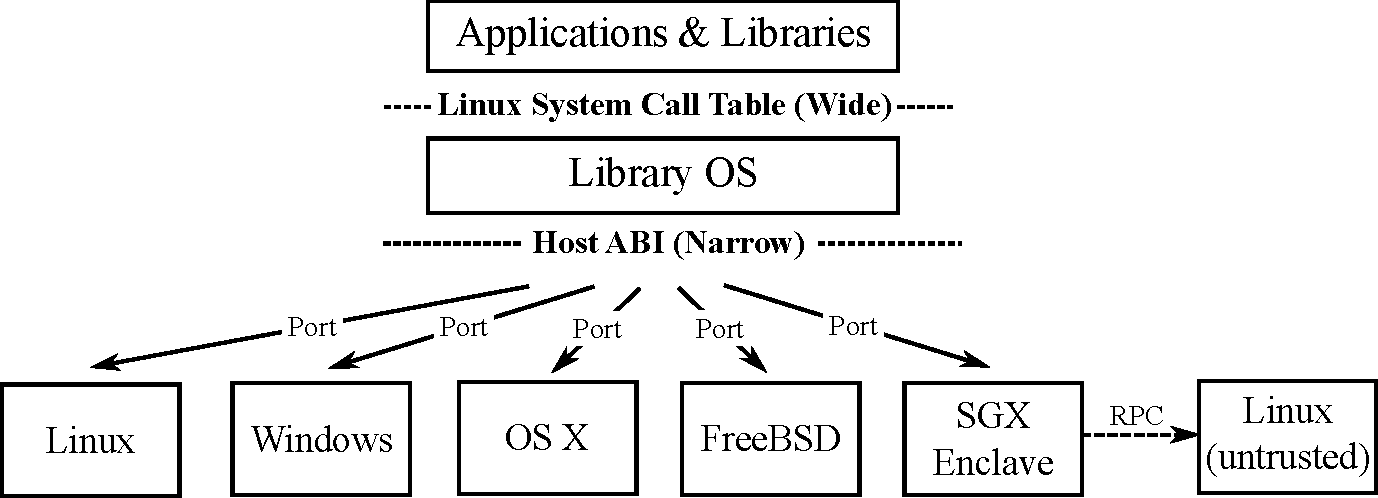
\includegraphics[width=30em]{porting.pdf}
\caption{Porting model of \graphene{}.}
%\vspace{-.1in}
\label{fig:overview:porting}
\end{figure}



\papersubsection{Platform Adaption Layers (PALs)}
\label{sec:overview:host:pal}


For each host OS or hardware, \graphene{} uses
a thin library called a {\bf platform translation layer (PAL)}
to translate among host interfaces.
%is loaded below the library OS, to translate each functions in \thehostabi{} to native system interfaces.
The main purpose of a PAL is to mitigate the semantic gap
between \thehostabi{} and
native host system APIs.
%The effort of PAL development is per host OS, whereas the library OS implementation is reusable on every hosts. %The simplicity of \thehostabi{} can be also estimated by the effort of implementing a PAL for each host.
By implementing a PAL on a new host OS or hardware,
users can reuse
the same \libos{} to run the same collection of unmodified Linux applications.
%To keep the porting effort low,
%the development of a PAL must be straightforward
%for average OS developers.
%to achieve with limited efforts.
%Based on the principle of porting simplicity, PAL development must be straightforward
%for average developers.







%The host ABI is defined for the simplicity of porting, as well as the sufficiency for implementing a library OS compatible to Linux.
%First of all, the number of host functions included in \thehostabi{}
%is much smaller than the number of system calls in a commodity OS such as Linux. 
\graphene{} currently contains PAL implementations for several popular OSes,
including Linux, \win{}, \osx{}, and FreeBSD.
%and \sgx{} with an untrusted Linux kernel.
Most of these OSes provide a POSIX-like system API similar to \thehostabi{}.
Due to the similarity, translating most of \thehostabi{} to one of the system APIs
are straightforward for average OS developers.
\Thehostabi{} is also much smaller than the actual POSIX API, making it extremely portable.



A part of \thehostabi{} may be challenging to port
on an OS,
due to unexpected system assumptions made by the OS.
For instance, \win{} does not support
fine-grained memory deallocation for de-privileged applications.
To implement system calls like \syscall{munmap} and \syscall{mprotect},
\graphene{} needs host ABIs to
deallocate or protect virtual memory pages at page granularity.
%A workaround is to change memory mappings at the physical page level,
%but will require running the \win{} PAL with root permissions.
%This type of porting challenges
%tends to be results of design decisions or assumptions made by OS developers.
%A \libos{} can potentially design
%different emulation strategies
%to compensate missing host abstractions.
A few host abstractions such as a bulk IPC feature are
optional to the host ABI;
if a host OS does not support these abstractions,
the \libos{} must fall back to alternatives. 

%In our experience, the development of a PAL is around ten thousand lines of code.

%For each port, the amount of code written for implementing \thehostabi{} is at the order of magnitude of thousands of lines of code, which is much more manageable than implementing a flat translation layer for system interfaces.


\begin{comment}
Based on the experience in \graphene{},
it is hard to ensure the portability of \thehostabi{} on every potential hosts.
%even a host ABI specialized for simplicity cannot guarantee to be portable on every hosts.
A host may simply lacks the functionality
for implementing a \hostapi{}.
The assumption is, maintaining the compatibility of \thehostabi{} poses a much less challenge than maintaining the whole system API.
Besides, the library OS may flexibly switch among emulation strategies
to compensate the absence of certain host abstraction.
As an example,
bulk IPC is optional in \thehostabi{} since its first definition,
due to the expectation
that implementing the feature may not be feasible on some hosts.
If bulk IPC is not available,
the library OS can fall back to RPC-based IPC, with a reasonable amount of performance penalty.
In the worst case, if there is no emulation strategies
to compensate for the absence of a \hostapi{},
user can predict the affected applications and avoid running these applications
on specific hosts. 
%at least users can predict whether an application will be affected and thus cannot run on certain hosts.
\end{comment}


%For a host OS that does not support ELF binaries, the PAL must follow the binary format which the host OS accepts, such as the Portable Executable (PE) format on \win{}.
%The PAL is the only layer in the user space which cannot be reused
%across different hosts. Besides the PAL, all of the other binaries in the user space are fully reusable, including the library OS, the supporting libraries, and the application executable.



%The host abstractions map to several common system calls in a commodity OS.
%For example, \funcname{StreamRead} and \funcname{StreamWrite} can directly map to the POSIX functions \funcname{pread} and \funcname{pwrite}, which are available in most OSes including Linux, BSD, \osx{}, and \win{}.
%More than half of the functions in \thehostabi{} can be counted toward this category.
%The rest of the host abstractions are either specific to Linux
%(e.g., TLS support),
%or belong to the POSIX functions that are not shared with commodity OSes
%(e.g., \funcname{mmap} on \win{}).
%The PAL emulates these host abstractions, using existing system interfaces available on the host OS, unless the software emulation is fundamentally impossible (e.g., restricted by the system interfaces), or too expensive (e.g., high overhead from copying data).



\papersubsection{Definitions and design principles}
 

\graphene{} defines \palcallnum{} calls in \thehostabi{} (also called \hostapis{}),
with a set of host abstractions
sufficient for \libos{} development.
%The host ABI defines the interaction between the library OS and a specific host.
%The \graphene{} library OS can be deployed on any ``host'' where \thehostabi{} has been ported.
This thesis defines
a {\bf host} of \thehostabi{}
to be an OS or hypervisor
which contains enough OS functionality for running a standalone application or virtual machine.
Most of the host targets in \graphene{}
are monolithic OSes,
including Linux, \win{}, \osx{}, and FreeBSD.
%which has defined a massive system API for programmability.
A monolithic OS 
usually contains a massive amount of system APIs,
which is sufficient for
implementing \thehostabi{}.


A special example of a host
is an \sgx{} (Software Guard Extensions) enclaves~\cite{intelsgx},
which
restricts OS functionality for security reasons.
The restrictions on \sgx{}
are results of a strong threat model
which distrusts any OS features except ones that are virtualized by the CPUs or migrated into enclaves.
The only way to obtain any missing OS features such as storage or networking
is to request through RPC (remote procedure call).
Requesting untrusted OS services through RPC also introduces new security threats that application developers tend not to anticipate~\cite{checkoway13iago,osdi16scone}.
Due to all the compatibility and security challenges discussed above,
this thesis uses \sgx{} as a representative example of a host
with unusual assumptions (e.g., threat models) and restrictions
compared to a monolithic OS.

%An innovative hardware abstraction like \sgx{} (software guard extensions)
%imposes unique assumptions and restrictions
%on a commodity OS,
%%creates a special host on top of Linux or \win{},
%%with unique interfaces and specifications regarding the host OSes.
%and thus creates a special host above the OS.

%If an OS has mutated or tweaked the interface for a hardware platform,
%such as an \sgx{} enclave 
%running on an untrusted Linux kernel,
%the combination of the OS (Linux) and the hardware platform (\sgx{}) is considered a specialized host.
%Especially, the \sgx{} port of \thehostabi{} faces several unique challenges,
%which will be discussed in Chapter~\ref{chap:sgx}.


\begin{comment}
%\fixme{each sentense should be a paragraph; starting the 2nd sentence}
\fixmedp{start with a strong opening stating the rationale}
The host ABI of \graphene{}
define functions needed from a host, in order to implement the library OS for reusing applications.
%to reuse an application and all its supporting libraries, including the \graphene{} library OS.
Each host of \graphene{} contains an OS and a hardware platform, either of which causes compatibility issues for running unmodified applications.
OS developers can port the library OS to a new host,
by simply reimplementing the narrowed host ABIs using abstractions available on the host.
%a new host platform.
%For each host which requires the compatibility for unmodified Linux applications, one only has to implement the narrowed host ABIs,
%instead of reimplementing the bloated, ``legacy'' system interfaces
%needed by the applications.
By implementing \thehostabi{}, OS developers skip the painful process of rebuilding the whole system interfaces of a commercial OS such as Linux.
The host ABIs strictly decouples the porting effort on the hosts from the compatibility feature for applications.
%The host ABIs decouple the OS development in the host and the implementation of compatibility for the existing Linux application.
What \thehostabi{} exposes is a simplified extended machine,
similar to a para-virtualization interface, capable of running the library OS as a lightweight virtual machine. % with compatibility against Linux applications.
%on which another layer of virtualization (i.e., the library OS) can be built to reproduce the compatibility for Linux.
\end{comment}


\begin{comment}
Two design principles drive the definition of \thehostabi{}s:
{\em simplicity} (i.e., easy to port on any hosts)
and {\em sufficiency} (i.e., containing enough OS functions for implementing a library OS).
The process of deciding \thehostabi{}s is comparable to
finding a ``pinch point'' within a OS implementation,
which can conveniently mediate a significant portion of OS execution paths for managing hardware abstractions.
%The two principles drive the development of \thehostabi{}s,
%The whole development of the \graphene{} library
%must be disciplined
%on extending \thehostabi{}s only when it is strongly required.
%of restraining extensions to \thehostabi{}s unless absolutely necessary.
The two principles
determine the soundness of the \graphene{} approach to improving compatibility
for any hosts.
\end{comment}


%%The host ABI is defined with partitioning in mind.
%\Thehostabi{} 
%determines a boundary which partitions several upper-level OS components, %, such as system calls and namespaces,
%into a library OS,
%%, as a dynamically-linked library which can be deployed
%%to various hosts.
%%The rationale behind the partitioning is based on the fact that not every OS component is equally important to compatibility, for applications which need to be ported across hosts.
%%When an OS is extended for a new hardware,
%%these OS components usually remain unchanged, or are predominantly reused.
%%Partitioning
%%into a library OS further guards these 
%in order to isolate the host idiosyncrasy. % on specific hardware. %any potential changes for adopting new hardware.
%%Similar isolation
%%exists in traditional OSes, but without partitioning:
%The strategy
%is also used in OSes:
%An example is the Linux virtual file system (VFS), an internal interface
%which encapsulates operations of file system drivers.
%%On the other hand,
%%drivers (e.g., drivers for file systems, block devices, or network cards)
%%and architecture-specific instructions
%%stay encapsulated in the host OS.
%%in the Linux kernels are usually encapsulated under a virtualized, in-kernel interface (e.g., the Linux virtual file system),
%%to simplify the development of the rest of the kernel.
%Similar to VFS,
%\thehostabi{} is intended
%to be a more ubiquitous interface,
%which encapsulates
%any host-specific behavior and semantic
%inside the host OS.
%%for encapsulating both OS and hardware idiosyncrasy on a wide range on hosts.
%%declares a ubiquitous system interface, to encapsulate both OS and hardware abstractions
%%for the library OS.




\Thehostabi{} shares several characteristics with a virtual hardware interface
exported by a hypervisor.
A generic, backward-compatible
virtual hardware interface
%a set of generic, virtual hardware,
%which the VM can control with the same drivers.
allows an unmodified OS kernel to run inside a virtual machine as on the bare metal.
%by exporting interfaces close to commodity hardware.
%To avoid additional porting effort, the virtual hardware are close to the typical commodity hardware.
%For instance, a virtual hardware interface
%usually includes a virtual NIC (network interface controller),
%such as the virtualized E1000 interfaces
%available in VMware workstation or QEMU.
%As a result, \thehostabi{} contains the
%typical OS features and interfaces, similar to the API of early UNIX systems.
The key difference between
a virtual hardware interface
and \thehostabi{}
is that \thehostabi{} does not target reusing a whole, unmodified OS kernel as a guest.
Instead, 
\thehostabi{} contains higher-level abstractions such as files and network sockets
to ensure portability on most host OSes.
The concept
of defining \thehostabi{}
with a customized guest OS (i.e., a \libos{}) running atop \thehostabi{} is similar to para-virtualization.
%\thehostabi{} expects the \libos{}
%to be rewritten and
%customized for \thehostabi{},
%similar to a 
%para-virtualizated VM.
%Compared to an actual para-virtualized VM,
A para-virtualized VM defines hypercalls as interfaces between a guest OS and a hypervisor.
Furthermore, \thehostabi{} avoids duplication of OS components
such as scheduler, page fault handler, file systems, and network stacks
between the host and \libos{}.
%Another difference is that \thehostabi{} is called by normal function calls, whereas para-virtualization relies on hypercalls.
To compare a VM and a \libos{} on a spectrum,
a VM reuses a whole OS on a wide, backward-compatible virtual hardware interface
whereas a \libos{} implements only system API components on a simplified host ABI.

The following paragraphs discuss the key design principles of \thehostabi{},
including porting simplicity, sufficiency for \libos{} development, and ease of migration.

\paragraph{Porting simplicity.}
%To reduce porting effort
%\thehostabi{}
%must be simple to port on a host OS or hardware.
To reduce porting efforts,
\graphene{} defines \thehostabi{}
using two strategies:
first, \graphene{} significantly reduces both the size and complexity of host OS features
that OS developers have to implement.
Effectively, \graphene{} avoids duplicated OS features and handling rare corner cases
on \thehostabi{}.
%The development of \graphene{} disciplinarily avoiding adding any functions to \thehostabi{},
%unless the library OS cannot internally implement an OS feature.
Second, the definition of \thehostabi{}
imitates common system APIs in a POSIX-like monolithic OS,
to directly translate most calls to
a few similar host abstractions.
%existing system calls or system library functions
%on each host.
%include functions which can be directly mapped to OS functions exported by the host.
%%the likelihood of finding similar features on the host, to be translated to functions in \thehostabi{}.
%The assumption that such a strategy is possible
%is based on
%the observation that
%%similarity of system interfaces is common among most OSes.
%similar OS functions, especially UNIX-style APIs,
%tend to commonly exist in most OSes.
%, to reduce the learning curve for programming applications.
For instance,
the stream APIs in \thehostabi{}, such as \palcall{StreamRead} and \palcall{StreamWrite}
are similar to
system calls like \syscall{read} and \syscall{write} exist on Linux, BSD, and POSIX API,
or \syscall{ReadFile} and \syscall{WriteFile}
on \win{}.
%with similar functionality and semantics.
%and 
%looks similar to \syscall{ReadFile} in \win{}, except the data types.
%The definition of \thehostabi{}
%is based on observations of the system interfaces in some of the important hosts,
%including Linux system calls and \win{} API.
%exported by the targeted hosts,
%and defines the functions in \thehostabi{}, to be easily translated to the native system interfaces.
%The host ABI is essentially a subset of the common features from every potential hosts.
%We expect %\thehostabi{} defined with simplicity in mind
%to be straightforward to port on most hosts,
%Most functions in \thehostabi{} can be easily translated to host system interfaces
%in various styles.
As the rest of this thesis proves, porting \thehostabi{} is straightforward
on most monolithic OSes.

%For example, \thehostabi{} defines \syscall{StreamRead} and \syscall{StreamWrite} for accessing I/O streams, similar to .
%xcept some nuanced details like order of parameters.


% by including OS functions , such as \syscall{FileRead} and \syscall{FileWrite}, similar to the Linux system calls, \syscall{pread} and \syscall{pwrite}.




\begin{comment}
The simplicity of \thehostabi{}s requires retaining a minimalist design of host functions. %, based on typical OS services for managing hardware.
%\graphene{} reduces the host functions
%to the bare minimum.
The host ABIs should only contain operations that
are absolutely necessary for requesting external hardware abstractions.
%A way to simplify \thehostabi{}s is to move host functions into the library OS
%and to replace them with wrappers consisting of other host functions.
Any functions that can be partially or wholly implemented inside the library OS
should be further simplified, or even removed from \thehostabi{}s.
%---in other words, whether \thehostabi{}s can be further reduced.
Moreover, \thehostabi{}s have to be simple enough to implement on
most hosts;
%In the simplest host ABIs, none of the host functions shall be able to internally implement the behavior of another host function,
%or the definition of \thehostabi{}s is further reducible.
that is, \thehostabi{}s should contain only OS functions that are commonly offered on
most hosts.
The host ABIs are close to simplified UNIX interfaces,
such as reading or writing a file or an I/O device as a byte stream,
or creating a virtual memory mapping.
%the most common OS functions
%offered on most of the potential hosts,
For most hosts,
implementing \thehostabi{} should be as straightforward as redirecting the functions to the closest host system calls.
%such as the Linux system calls or the \win{} APIs.
For example, the functionality of \syscall{StreamRead} and \syscall{StreamWrite} in \thehostabi{}s can loosely match with
\syscall{read} and \syscall{write} in Linux,
or \syscall{ReadFile} and \syscall{WriteFile} in \win{}.
%This thesis also evaluates the simplicity of \thehostabi{}s by counting the lines of code used to implement \thehostabi{}s on each host platforms.
Since most OSes have inherited a similar design from UNIX,
it is fair to assume finding
comparable OS functions %host platforms
to \thehostabi{} would be reasonably easy.
%fair to assume that \thehostabi{}s 
\end{comment}



\paragraph{Sufficiency for \libos{} development.}
%\Thehostabi{} defines
%the host abstraction available for a \libos{} to access host hardware abstractions.
To develop a \libos{} with compatibility against a wide range of applications,
\thehostabi{}
%are demonstrated by the fact that
%the exported host functions 
contain any OS abstractions that the \libos{} cannot easily emulate.
%and a full-function library OS is implemented on top of them.
For most hosts,
the host OS abstractions
%can be categorized into five types:
include
process creation, memory management, and I/O (typically, files and network connection)~\cite{dhamdhere2007os-textbook}.
%Besides security and protection,
%the definition of \thehostabi{} is closely related with hardware management,
%and offers the most basic abstractions for each category of OS functions.
%managing specific types of hardware,
%and each contain a few basic abstractions
%which can be expanded into other system interfaces.
%For example, the basic OS functions for memory management include
%allocating (\syscall{VirtMemAlloc}),
%protecting (\syscall{VirtMemProt}),
%and deallocating (\syscall{VirtMemFree}) memory regions. % at certain granularity
%(usually in pages).
%These basic functions can be used to implement other forms of memory allocation,
%such as growing heaps with \syscall{brk}
%or allocating thread-private stacks.
%The definition of the \drawbridge{} host ABI is a hint, for creating a list of host abstractions necessary for the library OS, including streams, memory, threads, and processes. 
%If \thehostabi{}s are insufficient for implementing certain system interfaces, one may extend \thehostabi{}s with the missing functions,
%with the discipline to retain the simplicity of \thehostabi{}s.
%The extension to \thehostabi{}s must be d, to keep the extension minimal, and to avoid adding redundant functions.
%The implementation of the \graphene{} library OS demonstrates that
%\thehostabi{} is sufficient for implementing significant portion of Linux system calls.
For each type of abstractions,
a monolithic OS may define several variants of system APIs with similar functionality.
For instance, Linux provides two system calls, \syscall{mmap} and \syscall{brk}, both for memory allocation in a process.
\syscall{mmap} allocates larger memory regions with page granularity,
whereas \syscall{brk} simply grows a single, continuous heap space for more fine-grained allocation.
Many applications such as GCC~\cite{gcc}
switch among system API variants in case one of them is unavailable on certain OS distributions.
This thesis shows that,
by adopting only the semantics of one of these similar APIs or abstractions, the host OS can stay simple with
the \libos{} emulating the rest of APIs.
For instance, \thehostabi{} includes \syscall{VirtMemAlloc}
as a similar feature as \syscall{mmap},
which is sufficient to emulating both \syscall{mmap} and \syscall{brk}.



\graphene{} defines \thehostabi{} partially based on
\drawbridge{},
a library OS for single-process \win{} applications.
The host ABI of \drawbridge{} 
contains 36 functions,
%demonstrates that its host ABI is sufficient
%for running a library OS in which 99.7\% of code comes from the \win{} 7 source.
%The host ABIs of \drawbridge{} are later extended
%for running a Linux-based library OS called Bascule~\cite{baumann13bascule}.
and several works have ported the host ABI to different hosts,
including \win{}, Linux, Barrelfish, and \sgx{}~\cite{porter11drawbridge,baumann14haven,mssql-on-linux,baumann13bascule}.
%and is capable of running a library OS for single-process, Linux applications, with a few host ABI changes~\cite{baumann13bascule}.
%ill loads and links the rest of application binaries, just like the native Linux loader (i.e., \code{ld.so}).
%\graphene{} takes the high-level definitions of the \drawbridge{} and Bascule host ABIs, and customizes for general-purpose Linux applications and a wider range of hosts. 
Although running \win{} and Linux applications may face
a different set of challenges,
the nature of their APIs is mostly similar, with a few exceptions.
During the development of \graphene{}, developers found the occasions in which
the host ABI of \drawbridge{}
is not sufficient to address Linux-specific challenges
and decide to extend \thehostabi{}.
Section~\ref{sec:overview:host:abi} and Chapter~\ref{chap:abi}
will further discuss the Linux-specific extensions of \thehostabi{}.


\paragraph{Migration.}
The \graphene{} library OS shares several features of VMs, including checkpointing and migrating a running application.
Migrating a process is also the key to emulating copy-on-write forking,
on a host without physical memory sharing (e.g., \sgx{}).
A hypervisor checkpoints and migrates a VM by snapshotting the VM states above a stateless virtual hardware interface. % as a clean boundary for snapshotting the application and OS state.
\Thehostabi{} is also defined to be statelessness,
by ensuring any states in the hosts to be temporary and reproducible to the applications and \libos{}.





\papersubsection{The \hostapis{}}
\label{sec:overview:host:abi}


%\fixmedp{the beginning doesn't capture the whole paragraph.}
%The host ABI shares several common abstractions with production OSes.
%The functions in \thehostabi{}
%define the basic features needed from the hosts, to run the library OS.
%The definition of the host functions
%should be unsurprising to average OS developers,
%making the implementation on a new host to be fairly straightforward.
%The host ABI reflects the common functionality of most OSes, including Linux and \win{}.
%Although the same OS abstractions may be defined
%as different idiosyncratic system interfaces on each host OSes,
%\graphene{} takes into consideration of porting the host functions to either OSes, in the most effortless way possible.





%fixmedp{give more of the background}
Table~\ref{tab:overview:abi} lists the \palcallnum{} calls defined in \thehostabi{}:
%Among these \hostapis{}, 
25 calls are inherited from the \drawbridge{} host ABI,
including functions to managing I/O (e.g., \palcall{StreamOpen}), memory allocation (e.g., \palcall{VirtMemAlloc}), scheduling (e.g., \palcall{ThreadCreate}), and several miscellaneous functions (e.g., \palcall{SystemTimeQuery}).
%Most of the host functions only affect the OS or hardware states
%related to the process itself.
%For example, \syscall{VirtMemAlloc} can only allocate memory in the calling process,
%and cannot affect other processes running in parallel.
%Only I/O streaming functions export states to the host OS, and share states with other processes or library OSes.
14 calls are added by \graphene{}, to implement Linux-specific features.
For example, unlike \win{} or \osx{}, Linux %The host ABI is also complemented with several Linux-specific abstractions, such as
delivers hardware exceptions to a process as signals.
Linux also requires 
the x86-specific segment registers (i.e., FS/GS registers)
to determine the location of thread-local storage (TLS), which can be hard-coded in application binaries by a compilation mode of GCC.
On \win{} or \osx{}, the x86-specific segment registers are mostly ignored, and even frequently reset to eliminate attack vectors.
%The host ABI contains host functions (), which can be directly called from the library OS. \graphene{} shows that \thehostabi{} is sufficient to implementing a large portion of the Linux system calls.
%These functions are not defined in \drawbridge{}, the \win{}-based library OS,
%because these abstractions do not exist in \win{}.
%The \drawbridge{} host ABI does not contain exception delivery because the feature is
%not commonly used in \win{} applications.
%Moreover, the x86 segment registers cannot be modified in \win{}
%because the OS assigns fixed values to these registers
%for the whole execution.
%Although \drawbridge{} excludes these abstractions, Bascule extends \thehostabi{} to include similar functions,
%demonstrating that the extension is indeed necessary.
\graphene{} discovers these abstractions as a necessity for implementing a rich Linux \libos{}.



\begin{table}[htp!]
\centering
\input{abi-table}
\caption{An overview of \thehostabi{} of \graphene{}. The ones marked with the symbol $\dagger$ are introduced in the initial publication of \graphene{}~\cite{tsai14graphene} or later extended for this thesis. The rest are inherited from \drawbridge{}~\cite{porter11drawbridge}.}
\label{tab:overview:abi}
\end{table}

%The interfaces, as part of \thehostabi{}, which access these host abstractions, are ultimately simplified to reduce the porting effort on each host.
%Unlike the system interfaces in the OS, \thehostabi{} does not prioritize backward compatibility. Therefore, \thehostabi{} includes only the minimum interfaces that the library OS needs to interact with the host. The host ABI does not have to include any of  the legacy system interfaces from a production OS, let alone preserving different flavors of system interfaces for backward compatibility.



\graphene{} introduces five calls for 
remote procedure call (RPC) between \libos{} instances
in a multi-process application.
\graphene{} simplifies porting multi-process abstractions
on each host OS
to implementing RPCs.
The basic RPC abstraction is 
a pipe-like RPC stream for message passing between processes.
To improve performance,
%RPC is critical for implementing the coordination of OS states
%across library OS instances.
%The basic form of RPC in \graphene{} is a pipe-like RPC byte stream, which a library OS can simply use to send messages.
%It is a common design choice
%to implement inter-process coordination through message-passing
%instead of shared memory, especially for hardware platforms that do not guarantee memory coherence~\cite{baumann09barrelfish}.
%A problem to the message-passing approach is the significant overheads
%on frequently exchanging distributed OS states.
\thehostabi{} defines an optional, bulk IPC abstraction
to send large chunks of virtual memory
across processes.
%The bulk IPC feature works similarly as sending the memory through RPC streams,
%but is much faster because it avoids copying memory in the host.


%for host platforms that urgently require lowering the RPC overheads.
%Another extension is for
%%\funcname{StreamSendHandle} and \funcname{StreamRecvHandle}
%delegating opened stream handles to another process, through a connecting pipe.
%The feature is similar to sending file descriptors
%through UNIX sockets in Linux, and is used to share opened network sockets with the \syscall{fork}'ed processes.
%%Another RPC abstraction is a bulk IPC channel; a process can use \funcname{PhsyicalMemoryCommit} to commit a large chunk of memory to a bulk IPC channel, which \funcname{PhsyicalMemoryMap} can map into another process, as copy-on-write. The library OS uses bulk IPC as an optimization to \syscall{fork}.
%Despite that either of the RPC primitives
%is not necessary easy to implement on every hosts, the inclusion of these host functions is completely optional, and the library OS can always fall back to the message-passing approach.



%All the host functions are designed to appear as ``stateless''
%as possible to the library OS.
%Being stateless to the library OS means that
%a host function does not preserve any permanent state of certain host abstraction.
%A stateless function can recover
%from disconnection of the library OS, and be reconnected at any timing.
%The host functions can maintain temporary bookkeeping for the convenience of porting,
%but should not assume the bookkeeping states to be permanent.
%The principle of defining all the host functions to be stateless
%is primarily for two purposes:
%{\em migration} and {\em security isolation}.
%For migration, the fact that the library OS can disconnect freely from the host functions simplifies the implementation of the migration feature.
%Migration is also an important foundation to implementing \syscall{fork}, because the cloned process need to receive a snapshot of the parent process.
%For security isolation, 
%a stateless host function is easier to check,
%because the security monitor only has to verify each instance of host function calls,
%instead of tracing multiple host functions over a longer period of time.

%the functions to access each host abstraction must appear \fixmedp{clarify `stateless'} stateless to the host, except for the handles to identify the resources. Each call to the host functions is independent. The arguments given for each call must be always be absolute values, instead of relative values.
%For example, the offset given to \funcname{StreamMap}, \funcname{StreamRead}, and \funcname{StreamWrite} (if the opened handle is a file) are offsets from the beginning of the file, and thus are irrelevant to how many bytes that are previously written or read.
%When enforcing isolation rules, the host OS can check the arguments of each calls to the host functions, independently and atomically.


%A host ABI (application binary interface) has to define the convention of application binaries, including the binary format and the linking procedure, as well as a set of  system interfaces.
%The host ABIs contain a minimal loader which recognizes a basic version of the ELF (Executable and Linkable Format), just enough to compose a binary of the library OS.
%The very initial loading procedure as part of \thehostabi{}s only loads a clean library OS instance.
%Each host of \graphene{} is supposed implement a minimal dynamic loader,
%which can load the \graphene{} library OS binary in ELF.
%The library OS then completes the dynamic loading procedure,
%by directly loading the Linux native dynamic loader (i.e., \code{ld.so}), and indirectly loading the rest of the application binaries.







\papersubsection{Host-enforced security isolation}
\label{sec:overview:host:security}


To target multi-tenant environments, 
\graphene{} enforces strong security isolation between mutually-untrusting applications running on the same host.
The security isolation of \graphene{} is comparable to running each application
in a VM or a container.
Just as a virtual hardware interface isolating each VM,
\thehostabi{} also enforces security isolation between library OS instances.
%according to the trust model of the applications.


On a trusted host OS,
\graphene{} delegates security isolation as a host-level feature.
The library OS and the application must mutually trust each other, due to lack of internal privilege separation in a process.
%The host ABI also separates API implementation
%from security isolation.
%To ensure isolation, each host must restrict access from the applications or the library OS, to any unauthorized host abstractions.
On each host, a reference monitor enforces security isolation policies, by access control on OS abstractions sharable among processes, including files, network sockets, and RPC streams.
%The host-level security isolation is orthogonal to API complexity.
Separating security isolation from API implementation simplifies security checks
for applications that only require
complete protection from other tenants.
%based on monitoring the references to host resources and rejecting authorized resource access.
%to the host abstractions.





%\graphene{} reduces the attack surface exposed to applications
%by restricting access to the host kernel ABI 
%and prevents access to unauthorized system calls, files, byte streams,
%and network addresses with a \emph{reference monitor}.
%The host kernel ABI exported by the \pal{} heavily 
%limits the ability of a \graphene{} application to interact with the rest of the system;
%any external interactions are further mediated by a reference monitor.
%Unlike a typical Linux system, \graphene{} applications cannot interact with shared 
%system daemons or other shared system resources.
%As a result, \graphene{} enforces security isolation similar to running applications in separate VMs---even
%applications that span multiple processes.


In \graphene{},
one or multiple processes of the same application run in a {\bf sandbox}.
Multiple library OS instances coordinate
in a sandbox
to present a unified OS view
to the application.
%As the library OS instances can coordinate shared OS states using simple RPC streams,
The design simplifies the enforcement of security isolation for multi-process abstractions.
\graphene{}
uses the reference monitor to block RPC streams across the sandbox boundary,
stopping applications in different sandboxes from accessing multi-process OS states.
%\graphene{} contributes a multi-process security model 
%based on the abstraction of a \emph{sandbox},
%or a set of mutually trusting processes.
%If a reference monitor exists, the reference monitor permits the processes within the same sandbox to communicate and exchange RPC messages, but disallows cross-sandbox communication.
The current design focuses on security isolation, although we do expect to extend the design for more sophisticated policies
in the future.

\begin{comment}
The only host abstractions that are shared across processes and must be mediated by the host for isolation are files, network sockets, and RPC streams
--- all other allowed host ABI modify only local process state, such as VMAs and threads.
%Thus, the reference monitor need only mediate file access, socket and RPC stream creation.
%an unprivileged daemon
%as well as extensions to the App\-Armor LSM~\cite{apparmor},
%which checks file and socket policies in the kernel.
%, reducing context switching overhead
%and the risk of race conditions~\cite{garfinkel03traps}.
In order for the reference monitor to restrict file access, socket and RPC stream creation,
each application includes a {\em manifest file}~\cite{hunt07rethink},
which describes a {\tt chroot}-like, restricted view of the local 
file system (similar to Plan 9's unioned file system views~\cite{pike90plan9}),
%including read-only shared files,
as well as {\em iptables}-style~\cite{iptablesman} network firewall rules.
To facilitate sharing read-only libraries, a manifest may specify a file system view which combines several different sub-directories of the local file system, and can prevent writing to files or directories.


For example, the \graphene{} reference monitor on the Linux host is implemented using \syscall{ioctl} to a special device (\code{/dev/graphene})~\fixme{a prospective design}.
A process is restricted by the Linux BPF-style system call filter, or the SECCOMP filter~\cite{seccomp}, to use \syscall{open} to access any files, or to \syscall{connect} or \syscall{bind} to any sockets.
It must use the \graphene{} special device to open or create streams, so the file paths or network addresses can be checked against the sandbox rules. The kernel module as the driver of the \graphene{} special device can coexist with any Linux Security Module (LSM), such as AppArmor~\cite{apparmor} or SELinux~\cite{selinux}.


When a new process is launched by the host, it begins execution in a new sandbox.  
Child processes may either inherit their parent's sandbox, or can be started in a separate sandbox---specified by a flag to the host abstractions of process creation.
A parent may specify a subset of its own file system view 
when creating a child, but may not request access to new regions of the host file system. 
%The restrictive policy enforced on the child will be written in a new manifest file generated by the parent, and the policy will be checked by the reference monitor.
The child may also issue an {\tt ioctl} call to 
dynamically detach from the parent's sandbox. The reference monitor prevents byte stream creation across sandboxes.
%among picoprocesses
%that are not in the same sandbox.
%and restricts external connections to remote URIs according to firewall rules in the manifest.
When a process detaches from a sandbox, effectively splitting the sandbox, the host must closes all RPC streams that could bridge the two sandboxes.
\end{comment}



\paragraph{Threat model.}
For most hosts, application trusts the host OSes as well a \libos{} instances in the same processes.
For multiple processes inside a sandbox,
the \liboses{} in these processes
also trust each other.
Applications or \liboses{} are not trusted by the host OSes or processes outside of the sandboxes.
Applications and \liboses{}
can become the adversary to the host OS,
by exploiting vulnerabilities on \thehostabi{}.
%the \graphene{} design reduces the attack surface between the hosts and the library OS instances, to defend against a malicious application.

%On a host with a reference monitor, the host OS and the reference monitor are both trusted, to mediate all system interfaces used to implement \thehostabi{}. The host must check all access to any abstractions with effects outside of a process's internal state, such as an opened file, or a connected network socket.
%Processes inside the same sandbox mutually trust each other. The adversary can run arbitrary code inside of one or more processes within one or more sandboxes.
%The adversary can control all code in its processes, including the library OS and the host-specific PAL.
%{\tt libLinux} and the \pal{}. 
%We also assume a trusted reference monitor process running on the host kernel that 
%launches \graphene{} applications and mediates all system calls with external effects,\fixmedp{define precisely}

%\graphene{} ensures that %The key security property the \graphene{} design upholds is that 
%the adversary cannot interfere with any victim picoprocesses
%in a separate sandbox.  
%The \graphene{} sandbox design ensures strict isolation: 
%if the only shared kernel abstractions are byte streams and files, 
%and the reference monitor ensures
%there is no writable intersection between sandboxes,
%the adversary cannot interfere with any victim picoprocess.


The threat model of \graphene{} on \sgx{}
contains the adversary from other hosts but excludes
the host OS, hypervisor, and any hardware except the CPU from its trusted computing base (TCB).
An untrusted OS or hypervisor
potentially has lots of opportunities to invade applications or VMs,
using Iago attacks~\cite{checkoway13iago}.
The challenges of porting \graphene{} to \sgx{} is not limited to resolving the compatibility issues of enclaves but also defending applications and \liboses{} against untrusted host OSes.







%%% The only processes allowed to run as standard kernel processes (non-\graphene{}) 
%%% are the reference monitor and
%%% system administration utilities that need more kernel interfaces than the \pal{} ABI provides.
%%% Ensuring that a collaborating picoprocess correctly implements
%%% some function (such as receiving a signal),
%%% as well as preventing exploitation of vulnerabilities in picoprocesses
%%% are beyond the scope of this work.

%\graphene{} reduces the system attack surface of the host, but does not change the size of its
%trusted computing base; however, reducing the effective system call table
%size of a picoprocess does facilitate adoption of a smaller host kernel,
%which we leave for future work.


\papersection{The \libos{}}
\label{sec:overview:libos}

This section gives the overview of \graphene{}, a library OS for reusing unmodified Linux applications
on \thehostabi{}.
%Existing library OSes have established reuse of single-process applications~\cite{porter11drawbridge}.
%The library OSes map a target system API, such as the Linux system calls, to abstractions in \thehostabi{}. %The reduction of host interfaces provides portability to various platforms that can translate the interfaces to host APIs or abstractions,
%and a narrower attack surface that developers can more likely reason about.
% and supporting data structures as library functions---mapping
%high-level APIs onto
%a few paravirtual interfaces to the host kernel.
%Recent library OSes improve efficiency over full guest OSes by eliminating duplicated features
%between the guest and host kernel,
%such as the CPU scheduler, or
%eliminating guest-level multiplexing code, as the library OS supports only one application;
%even compiling out unnecessary guest kernel APIs~\cite{unikernels}.
A \libos{} is comparable to a partial, guest OS running in a virtual machine.
However, compared with an actual virtual machine, the \libos{} design of \graphene{} and previous work~\cite{porter11drawbridge,unikernels} eliminates duplicated features between the guest to the host kernel, such as the CPU scheduler or file system drivers, and thus reduces the memory footprint.
%Library OSes have also been proven useful for reusing applications on new hardware platforms, such as \sgx{} enclaves~\cite{baumann14haven}.
%% dp: This sentence seems a little premature
%In recent works, library OSes provide rich OS features for isolated contexts while the host OSes are untrusted

%% Library OSes reduce the memory requirements of running a self-contained,
%% isolated application process
%% %guest \daniela{I would replaced guest by "isolated process or group of processes (a \libos{} instance)''}
%% by orders of magnitude
%% In a cloud computing environment,
%% increasing the number of applications per server has enormous
%% economic benefits.
%% Even on a desktop or portable system, \libos{}es can reduce the overheads
%% of sandboxing untrusted code and running applications
%% designed for another OS.

%Because library OSes execute within a VM \daniela{this phrase does not read good to me because (i) it might imply the picoprocesses need hypervisor support, as misunderstood by reviewer 1 and (ii) you already emphasized the drawbacks of leveraging a VM} or lightweight process ({\em picoprocess}~\cite{xax}),
%library OSes execute with

%% dp: Daniela, great suggestion!  We need to make this situation seem more
%%     like the sky will fall without our help
A principal drawback for prior library OSes is the inability to support multi-process applications. Many existing applications, such as network servers (e.g., Apache) and shell scripts (e.g., GNU makefiles), create multiple processes for performance scalability, fault isolation, and programmer convenience.
%These applications would benefit from the efficiency and security benefits
%of a library OS.
For the efficiency benefits of library OSes to be widely applicable,
especially for unmodified Unix applications,
library OSes must provide commonly-used multi-process abstractions, such as \syscall{fork}, signals, System V IPC message queues and semaphores, sharing file descriptors, and exit notification.
Without sharing memory across processes, the library OS instances must coordinate shared OS states to support multi-process abstractions.
%To support multi-process abstractions, library OSes often have to rely on sharing OS states,
%backed by the hosts' memory sharing features.
For example, \drawbridge{}~\cite{porter11drawbridge} cannot simulate process forking because copy-on-write memory sharing is not a universal OS feature.


\begin{figure}[t!]
\centering
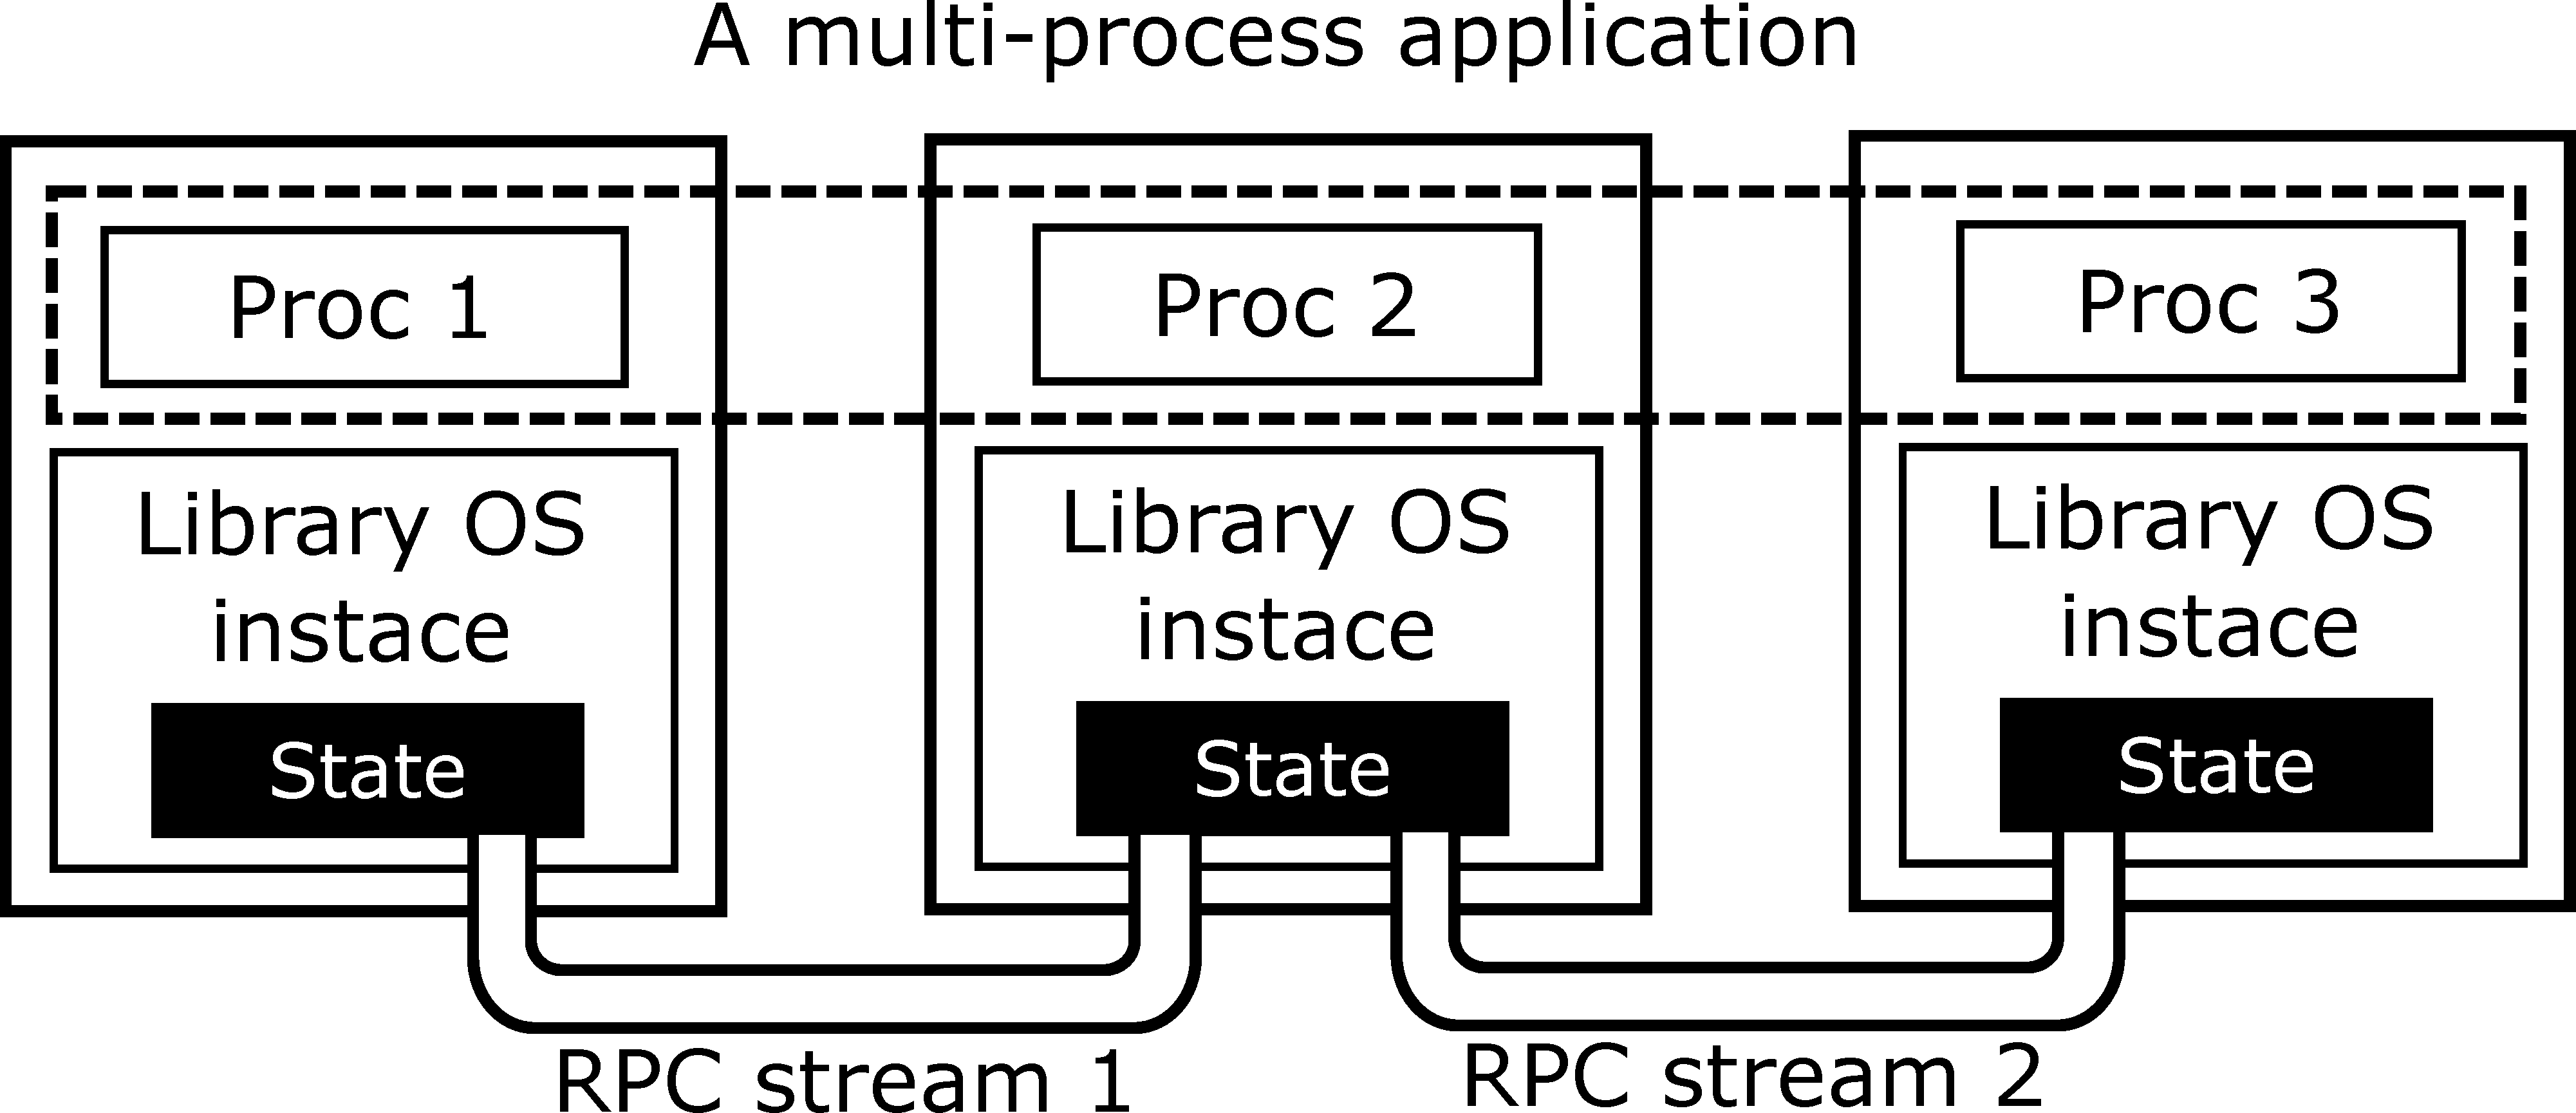
\includegraphics[width=24em]{concept.pdf}
\caption{Multi-process support model of \graphene{} \libos{}. For each process of an application, a \libos{} instance will serve system calls and keep local OS states. States of multi-process abstractions are shared by coordinating over host-provided RPC streams, creating an illusion of running in single OS for the application.}
%\vspace{-.1in}
\label{fig:graphene:concept}
\end{figure}

%{\bf \graphene{}} is a Linux-compatible library OS to run legacy, unmodified Linux applications. 
In \graphene{}, multiple library OS instances collaboratively implement
Linux abstractions, but present single, shared OS view to the application.
\graphene{} instances coordinate states
using message passing over RPC streams.
With a distributed POSIX implementation,
%placement of shared state and messaging complexity are first-order performance concerns.
%%We chose to shift implementation complexity into the library OS
%%in order to uphold simple enforcement of security isolation in the host.
%By coordinating shared states across library OS instances, 
\graphene{} can create an illusion of running in a single OS for multiple processes in an application.

%Previous library OS designs ensured security isolation of independent applications,
%comparable to a VM, by keeping a relatively narrow host ABI.
%We selected the \graphene{}
%design because it strikes a unique balance between
%and robust, flexible security enforcement.
%The \graphene{} design ensures security isolation of
%mutually distrusting, multi-process
%applications on the same host system.
%Essential to this goal is
%minimally expanding the host ABI to support multi-processing,
%as well as leveraging RPCs as a natural point to mediate inter-\picoproc{} communication.
%RPC coordination among \graphene{} instances can be dynamically disconnected, facilitating novel sandboxing
%techniques.  For instance, we develop an Apache web server extension that, upon logging in a given user,
%places the worker process's \libos{} in a sandbox with access to only that user's data.
%We expect more nuanced degrees of trust are possible in future work.

%\graphene{}'s design gives the user and system administrator a high degree of flexibility
%in isolating arbitrary groups of unmodified application processes,
%while upholding the efficiency and host compatibility benefits of recent library OSes.

%\fixmedp{After a complete draft is written, coalesce all goals and make sure they are addressed early on.  We are doing some scatter-shot motivation}


\papersubsection{\Libos{} architecture}
\label{sec:overview:libos:arch}

%Recent library OSes~\cite{porter11drawbridge,unikernels,baumann13bascule,osv}
%are designed for security and efficiency, but are limited to single-process applications.
%The security isolation of \liboses{} derives from 
%limited, explicit data sharing and 
%a narrow host interface.  
A \libos{} typically executes in either a para-virtualized VM~\cite{unikernels,osv}
% \daniela{I would have the use of a VM as a discussion topic in the end of the paper.}, 
or an OS process called a \emph{\picoproc{}}~\cite{porter11drawbridge,baumann13bascule}, with a restricted host ABI.
%The host ABI heavily restrict effects outside of the application's address space
%as a result, applications in a \picoproc{} have very little opportunity to interfere with each other,
%yielding security isolation comparable to a VM.
%The library OS deduplicates features for hardware management in both the guest and host kernels.
\graphene{} executes within a \picoproc{} (Figure~\ref{fig:overview:arch}),
which includes an unmodified application and its supporting libraries, which run alongside a library OS instance.
The \graphene{} \libos{} is implemented over \thehostabi{} designed to expose very generic abstractions that are easy to port on any host OS.
%Although the \graphene{} prototype  host kernel is Linux, 
%we adapt a host ABI from Drawbridge/Bascule,
%which has been previously implemented on \win{}, Hyper-V, and Barrelfish~\cite{porter11drawbridge,baumann13bascule,baumann09barrelfish}.
%The \graphene{} host ABI is
% summarized in Table~\ref{tab:abi} and discussed in more detail in \S\ref{sec:linux:pal}\fixmedp{if not cut...}.  
%which exposes only tens of simple host calls. \daniela{briefly define \picoproc{}: A \picoproc{} is unmodified application code running with a \libos{}.}


\begin{figure}[t]
\centering
\begin{minipage}[b]{1.25in}
\footnotesize
\raggedleft
Linux system calls \\
\graphenesyscallnum{} out of \linuxsyscallnum{}\\
\vspace{0.1in}
Host ABI \\
\palcallnum{} \hostapis{}\\
\vspace{0.2in}
\hostsyscallnum{} Linux system calls
\vspace{0.35in}
\end{minipage}
\hspace{-1.25in}
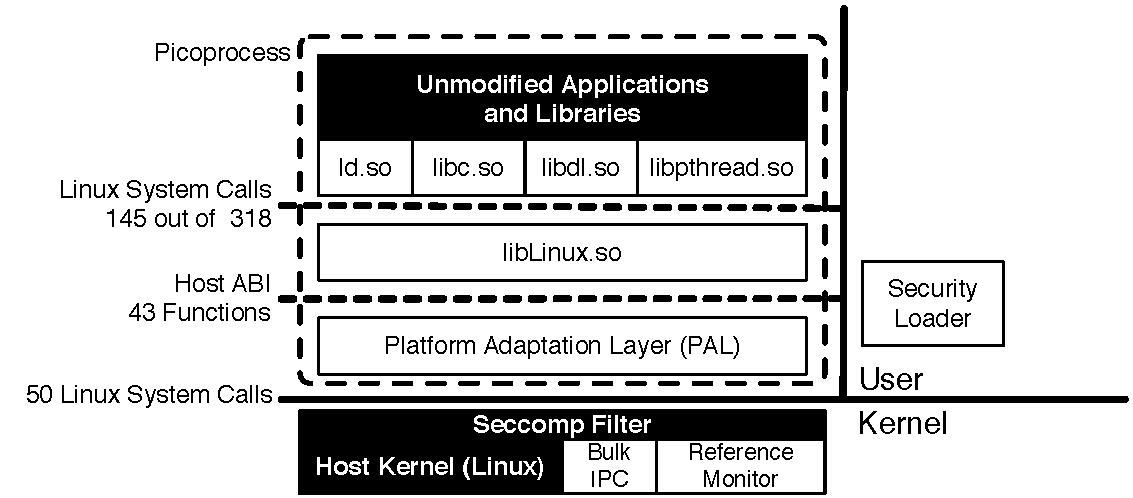
\includegraphics[width=32em]{arch.pdf}
\caption{Building blocks of \graphene{}.  Black components are unmodified.
We modify the four lowest application libraries on Linux:
{\tt ld.so} (the ELF linker and loader),
{\tt libdl.so} (the dynamic library linker),
{\tt libc.so} (standard library C),
and {\tt libpthread.so} (standard threading library), that issue Linux system calls as function calls directly to {\tt libLinux.so}.
Graphene implements the Linux system calls using a variant of the Drawbridge ABI, which is provided by the platform adaption layer (PAL).
A trusted reference monitor that ensures \libos{} isolation is implemented as a kernel module. Another small module is added for fast bulk IPC, but it is optional for hosts other than Linux.}
\label{fig:overview:arch}
\end{figure}


%\graphene{} shows the sufficiency of \thehostabi{} to support a rich Linux \libos{}.
As an example of this layering, consider the heap memory management abstraction. Linux provides applications with a data segment---a legacy abstraction dating back to original UNIX and the era of segmented memory. The primary thread's stack is at one end of the data segment, and the heap is at another.  The heap grows up (extended by \syscall{brk}) while the stack grows down until they meet in the middle.
In contrast, the host ABI provides only minimal abstractions for allocating, deallocating, and protecting regions of virtual memory.
This clean division of labor encapsulates idiosyncratic abstractions
in the library OS.


%These interfaces are host-independent \daniela{OS or kernel-independent}, as they tend to be very generic and easily
%implemented on any host OS kernel or VMM \daniela{postpone VMM for later}.

At a high level, a \libos{}
scoops the layer just below the system call table out of the OS kernel
and refactors the code as an application library.  
The driving insight is that there is a natural, functionally-narrow division point 
one layer below the system call table
in most OS kernels.
Unlike many OS interfaces, \thehostabi{} minimizes the amount of application state in the kernel, facilitating
migration. A \libos{} instance can programmatically read and modify its OS state, copy the state to another instance, and the remote instance can 
load a copy of this state into the OS---analogous to hardware registers.
A \picoproc{} may not modify another \picoprocs{}' OS states.



\papersubsection{Multi-process abstractions}
\label{sec:overview:libos:multiproc}


\issuedone{1.3.b}{An overview of multi-process support}
A key design feature of UNIX is that users compose simple utilities to create more significant applications.  Thus, it is unsurprising that many popular applications are multi-process---an essential feature missing from previous \liboses{}.
%This gap is filled by the \graphene{} \libos{}, which
%extends recent \liboses{} to support multi-process applications.
The underlying design challenge is minimally expanding a tightly-drawn isolation boundary without also exposing idiosyncratic kernel abstractions or re-duplicating mechanisms in both the host kernel and the library OS.

%requires a careful balance among the competing goals of 
%efficiency, host independence, and security isolation.
%The challenge, then, is minimal expansion of

%\vspace{5pt}
%\noindent {\bf Motivating Example.~}
For example, consider the process identifier (PID) namespace. In current, single-process library OSes, \syscall{getpid} could just return a fixed value to each application.
This single-process design is isolated, but the library OS cannot run a shell script, which requires forking and executing multiple binaries, signaling, waiting, and other PID-based abstractions.

%\paragraph{Design options.}
%Multi-process support requires extensions to the host ABI of recent, single-process library OS designs. Because multi-process abstractions, such as signals or System V IPC, tend to be idiosyncratic, an essential problem is identifying a minimal, host-independent substrate upon which  to implement OS-specific abstractions.
There are two primary design options for multi-process abstractions in \liboses{}: (1) implement processes and scheduling in 
the library OS; (2) treat each library OS instance as a process and distribute the shared POSIX implementation across a collection of library OSes.
\graphene{} follows the second option, which imposes fewer host assumptions.
%, maximize flexibility in mapping processes to physical resources, and facilitate inter-process security policy enforcement. % as enforcing security policies on related processes.

Multi-process abstractions
inside the library OS also possibly benefit from
hardware MMU virtualization, similar to
the model explored by Dune~\cite{belay12dune}.
However, this design reintroduces a duplicate scheduler and memory management.
Moreover, Intel and AMD have similar, but mutually incompatible MMU virtualization support,
which would complicate live migration across platforms.
None of these problems are insurmountable, and it would be interesting in future
work to compare both options.


In \graphene{}, multiple \liboses{} in multiple picoprocesses collaborate to implement shared abstractions. \graphene{} supports a rich of Linux multi-process abstractions including copy-on-write forking, \syscall{execve}, signals, exit notification, and System V IPC semaphores and message queues.
For instance, when process A signals process B on \graphene{}, A's library OS instance issues a query to B's instance over a pipe-like
RPC stream, and B's instance then calls the appropriate signal handler.
The host OS is unaware of the implementation
of multi-process abstractions,
as well as security isolation of the corresponding states.

%%% All collaborating \libos{} instances exchange messages as needed 
%%% to provide the application with a consistent view of 
%%% shared abstractions,
%%% such as


%\graphene{} approaches multi-processing by selectively replicating state and issuing remote procedure calls (RPCs) 
%%across multiple, collaborating
%library OS instances.
%Guests may work together to provide the unmodified multi-process application with
%coordination abstractions 

%%Shared abstractions on \graphene{}'s are implemented outside of the host, ensuring  host OS independence.
%% by implementing these
%%shared abstractions entirely
%%outside of the host kernel.
%%Shared abstractions are implemented outside of the host.
%%From the host kernel's perspective, 
%\graphene{} implements all shared abstractions by cooperatively managing the abstraction states over RPC streams.
%Single-process applications still service system calls from local state, and \graphene{}, includes optimizations to place state where it is most likely to be used, minimizing RPC overheads.
%The host reference monitor can easily isolate picoprocesses by 
%% \graphene{} design isolates \liboses{} by 
%%requiring all coordination to use 
%%explicit bytes streams \daniela{, pipe-like abstractions provided by the kernel. (suggestion: Reviewer  3)}.
%%Security isolation is enforced
%%by a kernel-level {\em reference monitor}, which can 
%%disconnect or prevent creation of a
%blocking all RPC messages, % between \liboses{} that should be isolated,
%without the need to understand the library OS details or semantics of these abstractions.
%In the PID example, only mutually-trusting picoprocesses can signal each other.
%%if the reference monitor prevents creation of RPC streams
%%across mutually untrusting \picoprocs{},
%%the \liboses{} cannot exchange signals.

%%% \graphene{} is designed to 
%%% The \graphene{} design leverages a number of optimizations to service application system calls 
%%% from local state whenever possible, and to minimize message passing overheads otherwise
%%%  (\S\ref{sec:namespaces:insights}).
%%% Our experience is that starting with a local system call design and then extending it to share state is relatively straightforward,
%%% and introduces little-to-no overhead when the request can be serviced locally.


The \graphene{} library OS is also capable of gracefully handling disconnection from other library OSes, facilitating dynamic application sandboxing.
RPC streams may disconnect at any time by either the reference monitor or at the request of a library OS.
%Message streams may be severed externally, by the reference monitor, or 
%one guest may simply disconnect from others to isolate itself.
%An application may disconnect itself from the 
%Any \graphene{} application may dynamically detach from the confederation, 
%or a host-level sandbox may dynamically separate two guests by severing their communication channels.
When a picoprocess is disconnected, the library OS will handle the subsequent
divergence, %and the library OS will will fork these abstractions
{\em transparently} to the application.
For instance, if a child process disconnect RPC streams from the parent by the reference monitor, the library OS will interpret the event as if the other process terminated, close any open pipes, and deliver exit notifications.
% \daniela{(applications run unmodified) - Reviewer 1 asked clarification on transparently}.

%% A key insight behind our design is that the common use case for these \daniela{cooperating} abstractions
%% is between a pair of processes.  Thus \graphene{} leverages a number of optimizations 
%% to reduce broadcast messages, avoid replication of needless state,
%% and service requests locally


\paragraph{Comparison with microkernels.}
The building blocks of \graphene{} are very similar to the system abstractions of a 
microkernel~\cite{liedtke95sosp,klein09sel4,elphinstone13microkernels,liedtke93sosp,chen93memory,baron1985mach-1,accetta86mach}, except a microkernel often has an even narrower, more restricted interface than the host ABI.
%such as the port and
%message abstractions of Mach~\cite{
A multi-server microkernel system, such as GNU Hurd~\cite{hurd} or Mach-US~\cite{stevenson95mach-us}, implements Unix abstractions across a set of daemons that are shared by all processes in the system. \graphene{}, on the other hand, implements system abstractions as a library in the application's address space and coordinates library state among \picoprocs{} to implement shared abstractions. \graphene{} guarantees isolation equivalent to running 
an application on a dedicated VM; it is similar to implementing the security isolation model on a multi-server microkernel by running a dedicated set of service daemons for each application.

%%% \graphene{}'s differences are motivated by two considerations: efficient support of both stand-alone, 
%%% single-process applications and multi-process applications; as well as flexible security isolation. 
%%% \graphene{} contributes techniques to seamlessly and efficiently transition 
%%% between single-process and multi-process support, as well as adapting 
%%% some known techniques to a new environment.

%The \graphene{} host ABI could be described as a hybrid microkernel, which also exposes the file system and network of the host kernel.
%Similarly, picoprocesses are assumed to be provided by a production OS, like Linux or \win{}, or by a Type 2 hypervisor.  A bare metal hypervisor could potentially export a PAL, but would require services from a trusted VM, such as Xen's dom0~\cite{barham03xen}.
%%or the \pal{} would implement more thread scheduling, networking, and file system code;
%%or the \pal{} ABI would change to push this code into the \libos{}.
%Arguably, recent library OS designs might be improved by rethinking the division of labor, but this is beyond the scope of this thesis.

%\paragraph{Alternatives.}
%Another approach to support multi-process applications in a library OS would be to use hardware MMU virtualization such as nested paging used by a system like Dune~\cite{belay12dune}
%in order to implement a second process abstraction, memory manager, and scheduler in the library OS.
%This approach threatens the efficiency benefits of deduplicating these features.
%A final option is exposing additional system interfaces, such as signals, by adding more system calls to a picoprocess. This approach undermines compatibility, as many of these coordination abstractions tend to be very OS-specific.
%%Unix signals vs.\ \win{} events, {\tt waitpid()} vs.\ blocking on a process handle, etc.
%%Although legacy OSes do enforce some access control rules on coordination abstractions,
%%kernel developers must audit and add hooks to millions of lines of code.
%%As a result,
%%users have lost confidence that a traditional OS can comprehensively enforce 
%%security isolation on these abstractions---a key motivation for using VMs
%%for security isolation.


%Systems must strike a careful balance between the competing goals of
%security isolation and multi-process coordination.
%Multi-process applications require OS-managed coordination abstractions such as signals, process exit notification, and System V IPC.
%These coordination abstractions operate within shared namespaces, such as the process ID namespace and the System V key space.
%These coordination APIs and namespaces must be consistent among coordinating processes, but can undermine security isolation among unrelated processes on the same host.
%System designs generally only meet one goal: traditional OSes have a rich but porous coordination interface, while sandboxing systems and VMs are strictly isolated.
%This thesis demonstrates that this unfortunate trade-off is not fundamental.
%coordination or isolation.  


%Traditional OS kernels typically provide  rich multi-process coordination APIs, but this richness also makes for a very porous attack surface area.  For instance, on \win{}, a program may inject libraries and create threads in another program~\cite{windows-dll-inject}; 
%similarly, unchecked file descriptor inheritance in Linux can lead to security problems~\cite{close-on-exec}.  
%Although legacy OSes do enforce some access control rules on these abstractions, kernel developers must audit and add hooks to so much code that users have lost confidence that an OS can comprehensively enforce security isolation on these abstractions.

%For achieving strong security isolation on applications, users have turned to VMs.
%For instance, if two customers host their websites in the same cloud service, the customers will insist on running their web servers in separate VMs for security.
%VMs take a heavy-handed approach to security isolation---ensuring that every application has a dedicated OS kernel in a hardware-isolated address space.
%Although virtual machines isolate applications and provide legacy OS abstractions within a VM, coordinating applications must be statically placed in the same VM,
%and cannot dynamically move to a separate VM.
%For instance, consider a web service running inside of a VM that wishes to isolate requests for different users in different VMs after authentication.  The web server administrator must statically create a VM for each user, introducing substantial
%overhead; and the developer loses convenient IPC abstractions and must rewrite large swaths of code.

\section{Summary}
\label{sec:graphene:summary}

The \graphene{} design is centered around
building a para-virtualized layer, which can reuse the OS components for reproducing Linux system interfaces.
%instead of building arbitrary compatibility layers for reproducing the system interface.
%constantly porting the significant  of the existing system interface.
%In \graphene{}, 
\graphene{} defines a host ABI, as a new boundary between the OS and user space.
The host ABI is simple enough to port (containing \palcalls{} functions),
and exports sufficient functionality for virtualizing a primary part of the system API components.
A library OS is built upon the host ABI,
and implements \graphenesyscalls{} Linux system calls to reuse unmodified Linux applications.
\graphene{} decouples the development for a compatibility layer,
from host-specific challenges to building OS features, and isolating applications from other malicious tenants.



%\sysname{} extends library OS designs 
%to include multi-process APIs required by common applications, such as a shell or 
%web server.
%\sysname{} demonstrates efficient, selective
%coordination of shared state across multiple library OS 
%instances---maintaining host independence.
%%simplifying security sandboxing of otherwise unwieldy OS features.
%Applications on \sysname{} enjoy both 
%strong security isolation with acceptable performance and low memory overheads.
%% from unrelated programs 
%%and seamless shared namespaces 
%%among a group of coordinating guests.
%%% Although this paper focuses on distributed coordination
%%% to facilitate the efficiency benefits,
%%% expect our experiences with distributed coordination 
%%% may also be particularly relevant to highly scalable OS designs, 
%%% which avoid the bottlenecks of shared OS data structures~\cite{baumann09barrelfish, song11eurosys}.
%%Graphene's overheads are acceptable and the memory 
%%footprint is substantially lower than a VM.



%% , which could benefit from the reduced memory footprint
%% in a cloud 

%% by introducing a novel design for  coordination APIs. 
%% to a new OS (Linux),
%% new classes of applications,
%% and introduces a
%% %an alternative design point for storage virtualization.
%% Our results further demonstrate the feasibility of the library OS model.
%% % generally,
%% Applications on Graphene enjoy both 
%% strong security isolation from unrelated programs 
%% and seamless shared namespaces 
%% among a group of coordinating guests.
%% Although we explore this concept in a library OS,
%% we expect the namespace coordination framework 
%% could also be adapted to limit the attack surface area between
%% processes in a traditional OS.
%% We expect these experiences with distributed coordination 
%% may also be particularly relevant to highly scalable OS designs, 
%% which avoid the bottlenecks of shared OS data structures~\cite{baumann09barrelfish}.
%and specifically of content-addressable storage as the primary virtual storage abstraction.
%%% This work opens up a number of interesting questions for future work, 
%%% including studying opportunities for low-level storage optimization within the CAS server,
%%% making CAS the root file system,
%%% eliminating storage management in the host kernel, and 
%%% investigating the impact of frequent migration among devices.

\begin{comment}
Enabling legacy applications in a restricted environment,
such as \picoprocs{} or enclaves,
requires extra effort for mitigating the limitations of platforms,
in order to support typical OS personalities.
\graphene{}, as described in this chapter, extends the existing \libos{} designs
from isolating single-process or unshared abstractions
to include multi-process APIs required by many UNIX applications,
such as servers or shell scripts.
The challenge that \graphene{} primarily overcomes
is the requirement for coordinating shared states across multiple \picoprocs{},
to provides a collaborative, unified OS view.
Essentially, \graphene{} implements all shared, multi-process abstractions
and OS states
based on coordination over host-provided, pipe-like RPC streams.
The RPC-based, distributed OS implementation enables multi-process support in \graphene{}, with minimal extension to the host interface,
and a sweet-spot for enforcing inter-application security isolation,
by simply sandboxing the RPC streams.
Such a model largely reduces the complexity of
enforcing security isolation
on idiosyncratic multi-process abstractions
and shared states.
Because the corporative nature of \picoprocs{} in \graphene{},
an application can even dynamically impose sandboxing on one of its processes,
to reflect per-process, variable security policies.
\end{comment}

\begin{comment}
In principle, we attempt to use \graphene{} to justify the platform independence
of the \libos{} design,
without sacrificing its qualitative benefits,
such as isolating mutually-untrusting applications
and a narrow attack surface to kernels.
\graphene{} implements a considerable number of common Linux system calls,
to support popular, modern applications
such as Apache web server, GNU Make, OpenJDK \java{} VM and the Python runtime.
\graphene{} translates the high-level system APIs used by applications
to a host ABI
inherited and extended from a previous Windows-compatible \libos{}~\cite{porter11drawbridge}.
In addition, we port the \pal{} (Platform Adaption Layer) of \graphene{}
to various platforms,
including FreeBSD, OSX, Windows, and even a more restricted environment, the \intel{} \sgx{} enclaves.
In particular, \graphene{} being ported to \intel{} \sgx{}
(\graphenesgx{})
can isolate applications --- either single-process or multi-process
--- on a host where neither the operating system nor the hardware (except the CPU package)
is trusted by the applications. 
Overall, \graphene{} shows that,
by simply porting the reasonably sized host ABI
to a new platform,
a whole large spectrum of legacy applications tested on the previous platforms
can be activated all together.
\end{comment}

\makeatletter
\def\input@path{{}}
\makeatother
\graphicspath{{}}
%\paragraph{Linux Personality.}

%\paragraph{Memory and Binary Loading.}

%\paragraph{Exception handling.}

%\paragraph{Attestation.}

%\paragraph{Framework Support.}


\subsection{Shielding Multi-Process Abstractions}
\label{sec:multiproc}

Many Linux applications use multi-process abstractions,
which are implemented using copy-on-write fork and in-kernel
IPC abstractions.
In SGX, the host OS is untrusted, and enclaves cannot share protected memory.
Fortunately, \graphene{} implements multi-process support
including {\tt fork}, {\tt execve}, signals, and a subset of System V IPC,
using message passing instead of shared memory.
%The {\it zero-sharing} nature of \graphene{} makes it possible
Thus, \graphenesgx{} implements multi-process abstractions in enclaves
without major library OS changes.
This subsection explains how
%we will describe how \graphenesgx{} securely creates
\graphenesgx{} protects
 multi-processing abstractions from an untrusted OS.


%% \fixme{need to polish this subsection}

%% Upon existing platforms using \sgx{}, there is no
%% multi-process abstractions of any kinds that has been supported so far,
%% either in \haven{} or other systems.
%% The main challenge against
%% implementing multi-process abstractions in enclaves
%% is to share enclave pages,
%% for either Linux-style copy-on-write {\tt fork}'ing or
%% sharing abstraction states.
%% Fortunately,


%processes in new enclaves,
%%for supporting
%        {\tt fork}, {\tt execve},
%and inter-process communication
%(namespace coordination, signals, System V IPC, etc)
%with process isolation.

%\subsubsection{Forking into new enclaves}
%\label{sec:multiproc:fork}

\begin{figure}[t!]
\centering
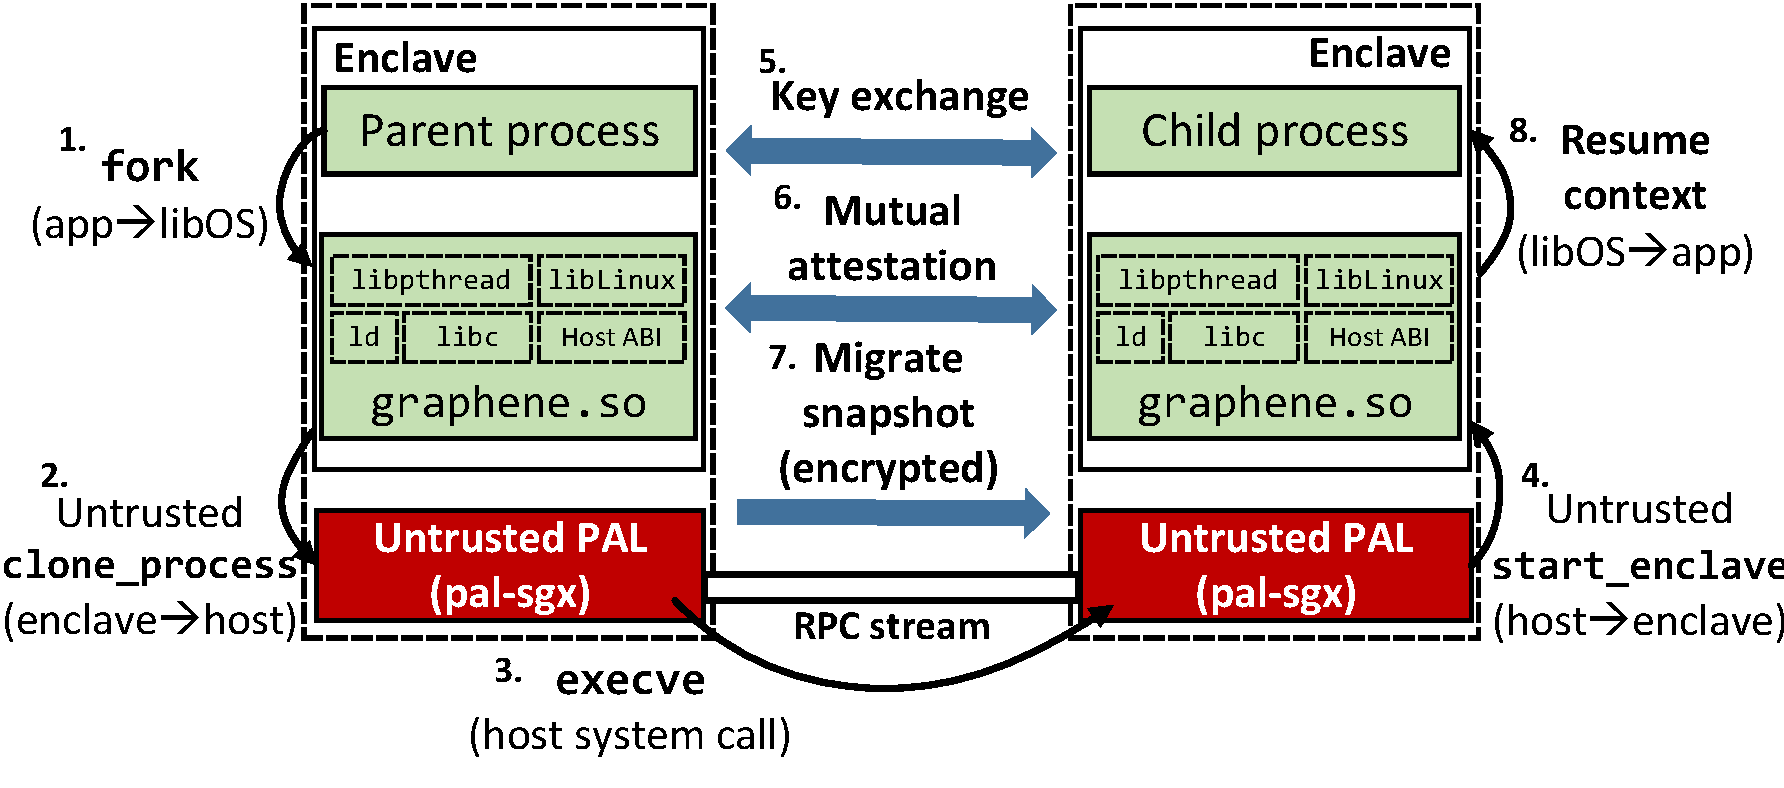
\includegraphics[width=\linewidth]{fork.pdf}
\caption{Process creation in \graphenesgx{}.
Numbers show the order of operations.
When a process forks, \graphenesgx{} creates a new, clean enclave
%calls {\tt execve} system call
on the untrusted host.
%to create a clean enclave with the same \libos{} image.
Then the two enclaves %build up the mutual trust by
exchange an encryption key, validates the CPU-generated attestation of each other,
and migrates the parent process snapshot.}
\label{fig:fork}
\end{figure}

\begin{comment}
To secure process creation across enclaves,
\graphenesgx{} is capable of building up the trust to newly launched enclaves,
through cooperation with an untrusted host.
Once a clean and trusted new enclave is launched,
The parent process will send a snapshot to the new one,
to create a clone of itself.
Snapshotting and migrating process states
is a feature robustly implemented and heavily used in \graphene{} \libos{},
of which we simply inherit the design.
\end{comment}

Process creation in \graphenesgx{} is illustrated in Figure~\ref{fig:fork}.
When a process in \graphenesgx{} forks into a new enclave,
the parent and child will be running the same manifest and binaries,
and will have the same measurements.
%\fixme{rewrite this part. check this. dp: check my rewrite}
Similar to the process creation in Graphene, the parent and child enclaves are connected with a pipe-like RPC stream, through the untrusted PAL.
As part of initialization, the parent and child will exchange a session key over the unsecured RPC stream, using Diffie-Hellman.
The parent and child use the CPU to generate attestation reports, 
which include a 
512-bit field in the report to store 
a hash of the session key
and a unique enclave ID.
The parent and child exchange these reports to authenticate each other.
Unlike remote attestation, local attestation does not require 
use of Intel's authentication service (IAS).
% then exchange attestation reports \fixmedp{right?} generated by the CPU (unlike remote attestation, local attestation does not require Intel-owned services to verify the CPU).
% which will prove that the attested enclave is the one and only one that agrees on the key.
% sensitive data from being divulged to an attacker during \syscall{fork}.
%For example, to prevent a man-in-the-middle attack, between the parent and child,
%we use
%a 512-bit field
%in the CPU-signed attestation to store a hash of the session key
%and a unique enclave ID, which will prove that the attested enclave is the one and only one that agrees on the key.
%generated and signed by \sgx{}.
%Once the child enclave is launched, as part of initialization,
%the parent and child will exchange attestation generated by the CPU,
%exchange a signed session key using Diffie-Hellman, and then 
%establish a TLS connection over an inter-enclave RPC stream.
% after creating a signed session key using a key exchange algorithm like Diffie-Hellman.
%then use a session key to generate an encrypted connection.
%\fixmedp{I still don't understand the following text; let's discuss}
%What the Intel CPU provides here is the confidential CPU secret that the inter-enclave attestation is based on. The attestation establishes a trusted path within enclave groups to exchange library OS state.
%\fixmedp{IF time, clarify what HW provides here or how it works}
Once the parent and child have authenticated each other, the parent establishes a TLS connection over the RPC stream using the session key.
The parent can then send a snapshot of itself over
the TLS-secured RPC stream, and the snapshot is resumed in the child process, making it a clone of its parent.
This mutual attestation and encryption strategy
% between the parent and child
prevents a man-in-the-middle attack between the parent and child.
%To build up the trust, the two processes will open an encrypted channel
%using a session key,
%and exchange attestation generated by the processor.
%Once both sides have confirmed the integrity of the other,
%the parent process is safe to send its snapshot, encrypted, to the child
%through the said channel.
%The child process will resume the snapshot in its own enclave,
%making it a clone of its parent.


%The fork design in \graphenesgx{} provides several security measures.
%First, mutual attestation and encryption between the parent and child
%prevent sensitive data from being divulged to an attacker during {\tt fork()}.
%To prevent a man-in-the-middle attack, between parent and child,
%we use
%a 512-bit field
%in the attestation structure generated and signed by \sgx{}.
%We use this field to store a SHA-256 hash of the session key,
%and a unique enclave ID,
%\fixmedp{also a piece of intuition missing here; let's discuss}
%to prove that the attested enclave is the one and only one that agrees on the key.

%% Forking in \graphenesgx{} mainly defends against 3 types of attacks
%% from the untrusted host:

%% \begin{compactenum}

%% \item The host pretends to be the child enclave, to expose the process snapshot
%% sent from the parent.

%% \item The host pretends to be the parent enclave, to compromise the
%% child process using a malicious process snapshot.

%% \item The untrusted host becomes a man-in-the-middle, which bounces
%% encrypted messages between the child and parent enclaves, with session keys
%% negotiated with both sides.

%% \end{compactenum}

%% As described earlier, attacks 1 and 2 are prevented by mutual attestation
%% between the parent and the child,
%% and encrypting the channel for sending the snapshot.
%% The attestation signed by the processor proves that both entities communicating
%% are valid \graphenesgx{} enclaves,
%% and encrypting the channel prevents the snapshot being eavesdropped or
%% counterfeited by the host.

%% To defend against attack 3 (the man-in-the-middle attack), we take advantage of
%% a user-customized 512-bit field
%% in the attestation structure generated and signed by \sgx{}.
%% This field is filled with a SHA-256 hash value of the agreed session key,
%% and the current enclave ID,
%% to prove that the attested enclave is the one who agrees on the key.

Once a parent enclave forks a child, by default, the child is fully trusted.
To create a less trusted child, the parent would need to sanitize its snapshot,
similar in spirit to the close-on-exec flag for file handles.
%to maintain its own security,
%because the migrated snapshot discloses all information in the parent.
%Unless the binary run in the parent enclave ensures
%that no secrets is stored in the enclave memory at the time of snapshotting,
%the parent enclave cannot simply drop the trust against the child.
For example, a pre-forked Apache web server may want to keep worker
processes isolated from the master %\fixmedp{Right nomenclature}, %that responds to HTTP requests isolated,
to limit a potential compromise of a worker process. %avoid being compromised by one attacked worker.
\graphenesgx{} inherits a limited API from \graphene{}, 
for applications to 
isolate themselves from untrusted child processes,
%\graphenesgx{} inherits this dynamic process isolation feature.
but developers are responsible for purging confidential information
before isolation.

\paragraph{Supporting \syscall{execve}.}

Unlike \syscall{fork}, \syscall{execve} 
starts a process with a specific executable, often different from the caller.
When a thread calls \syscall{execve} in \graphenesgx{},
the \libos{} migrates the thread to a new process,
with file handles being inherited.
%with clean process states except opened files cloned from the parent.
Although the child does not inherit a snapshot from its parent,
it can still compromise the parent 
by exploiting potential vulnerabilities in handling RPC, 
which are not internally shielded.
In other words, \graphenesgx{} is not designed to share library OS-internal
with untrusted children.
Thus, \graphenesgx{} restricts \syscall{execve} to only launch trusted executables, which are
specified in the manifest.


%  main challenge to supporting \exec{} is to
%ensure only trusted binaries can be created as child processes.
%loaded into new enclaves as child processes.
%The trust between parent and child must be mutual,
%or applications won't be secure.
%unless the two enclaves are strictly isolated.
%To secure \exec{},
%\graphenesgx{} stores the enclave measurements of executable binaries that can be trusted as children processes
%inside the manifest file.
%To identify binaries that can be trusted (either as parents or children)
%during process creation,
%\graphenesgx{} requires each binary ported for an application,
%to be shipped with a list of binaries that can be \exec{}'d,
%and those that can be callers of \exec{} to the said binary.
%Each binary in the list is identified by its measurement, which is mutually attested
%between the parent and the child during process creation.
%This list must be signed by a private key provided by the client,
%while the public key must be included in the enclave measurement of the binary.


\paragraph{Inter-process communication.}
\label{sec:multiproc:ipc}

After process creation, parent and child processes will cooperate
through shared abstractions,
such as signals or System V message queues, via RPC messages.
While messages are being exchanged between enclaves,
they are encrypted, ensuring that these abstraction are protected
from the OS.

%For \libos{}, OS states for these shared abstractions must be shared
%though inter-process coordination, for mainly two purposes.
%First, for each abstraction, \libos{} needs to maintain the state
%in one of its instances.
%Second, \libos{} must maintain the namespace states to identify and locate the
%abstraction states.
%\graphene{} implements a wide range of multi-process abstractions and namespaces,
%by coordinating OS state over RPC streams, rather than using shared memory. 

%% dp: this point already made above
%Because SGX does not allow enclaves to share trusted memory,
%the fact that the original Graphene design did not require shared memory
%made porting to SGX considerably easier.

% (pipes).
%Such a design is perfect for porting multi-process applications to enclaves.

%Thus, by coordinating OS state via 
%Thus, the benefit of coordinating OS state via message passing 
%is that 
%the enclaves need no will not share any memory to
%coordinate abstraction states,
%simplifying the support and security of library OS.
%and the RPC streams can be secured by the enclaves instead of the host.
%By encrypting the RPC streams among related processes,
%inter-process communication is easily protected from the untrusted OSes.
%In \graphene{}, security isolation among multi-process abstractions,
%regardless of their semantics,
%are enforced by isolating the RPC streams used for coordination.
%Unfortunately, \graphenesgx{} cannot trust the host to faithfully isolate
%the RPC streams.
%Each enclave launched for an application must secure inter-process coordination
%spontaneously, by only communicating to enclaves that it has attested
%and exchanged secret keys with.
%Because inter-process coordination is completely transparent
%to the applications,
%all information sent over RPC streams must be encrypted,
%because \libos{} cannot determine whether the information may contain any secret.






\section{Summary}
\label{sec:graphene:summary}

The \graphene{} design is centered around
building a para-virtualized layer, which can reuse the OS components for reproducing Linux system interfaces.
%instead of building arbitrary compatibility layers for reproducing the system interface.
%constantly porting the significant  of the existing system interface.
%In \graphene{}, 
\graphene{} defines a host ABI, as a new boundary between the OS and user space.
The host ABI is simple enough to port (containing \palcalls{} functions),
and exports sufficient functionality for virtualizing a primary part of the system API components.
A library OS is built upon the host ABI,
and implements \graphenesyscalls{} Linux system calls to reuse unmodified Linux applications.
\graphene{} decouples the development for a compatibility layer,
from host-specific challenges to building OS features, and isolating applications from other malicious tenants.



%\sysname{} extends library OS designs 
%to include multi-process APIs required by common applications, such as a shell or 
%web server.
%\sysname{} demonstrates efficient, selective
%coordination of shared state across multiple library OS 
%instances---maintaining host independence.
%%simplifying security sandboxing of otherwise unwieldy OS features.
%Applications on \sysname{} enjoy both 
%strong security isolation with acceptable performance and low memory overheads.
%% from unrelated programs 
%%and seamless shared namespaces 
%%among a group of coordinating guests.
%%% Although this paper focuses on distributed coordination
%%% to facilitate the efficiency benefits,
%%% expect our experiences with distributed coordination 
%%% may also be particularly relevant to highly scalable OS designs, 
%%% which avoid the bottlenecks of shared OS data structures~\cite{baumann09barrelfish, song11eurosys}.
%%Graphene's overheads are acceptable and the memory 
%%footprint is substantially lower than a VM.



%% , which could benefit from the reduced memory footprint
%% in a cloud 

%% by introducing a novel design for  coordination APIs. 
%% to a new OS (Linux),
%% new classes of applications,
%% and introduces a
%% %an alternative design point for storage virtualization.
%% Our results further demonstrate the feasibility of the library OS model.
%% % generally,
%% Applications on Graphene enjoy both 
%% strong security isolation from unrelated programs 
%% and seamless shared namespaces 
%% among a group of coordinating guests.
%% Although we explore this concept in a library OS,
%% we expect the namespace coordination framework 
%% could also be adapted to limit the attack surface area between
%% processes in a traditional OS.
%% We expect these experiences with distributed coordination 
%% may also be particularly relevant to highly scalable OS designs, 
%% which avoid the bottlenecks of shared OS data structures~\cite{baumann09barrelfish}.
%and specifically of content-addressable storage as the primary virtual storage abstraction.
%%% This work opens up a number of interesting questions for future work, 
%%% including studying opportunities for low-level storage optimization within the CAS server,
%%% making CAS the root file system,
%%% eliminating storage management in the host kernel, and 
%%% investigating the impact of frequent migration among devices.

\begin{comment}
Enabling legacy applications in a restricted environment,
such as \picoprocs{} or enclaves,
requires extra effort for mitigating the limitations of platforms,
in order to support typical OS personalities.
\graphene{}, as described in this chapter, extends the existing \libos{} designs
from isolating single-process or unshared abstractions
to include multi-process APIs required by many UNIX applications,
such as servers or shell scripts.
The challenge that \graphene{} primarily overcomes
is the requirement for coordinating shared states across multiple \picoprocs{},
to provides a collaborative, unified OS view.
Essentially, \graphene{} implements all shared, multi-process abstractions
and OS states
based on coordination over host-provided, pipe-like RPC streams.
The RPC-based, distributed OS implementation enables multi-process support in \graphene{}, with minimal extension to the host interface,
and a sweet-spot for enforcing inter-application security isolation,
by simply sandboxing the RPC streams.
Such a model largely reduces the complexity of
enforcing security isolation
on idiosyncratic multi-process abstractions
and shared states.
Because the corporative nature of \picoprocs{} in \graphene{},
an application can even dynamically impose sandboxing on one of its processes,
to reflect per-process, variable security policies.
\end{comment}

\begin{comment}
In principle, we attempt to use \graphene{} to justify the platform independence
of the \libos{} design,
without sacrificing its qualitative benefits,
such as isolating mutually-untrusting applications
and a narrow attack surface to kernels.
\graphene{} implements a considerable number of common Linux system calls,
to support popular, modern applications
such as Apache web server, GNU Make, OpenJDK \java{} VM and the Python runtime.
\graphene{} translates the high-level system APIs used by applications
to a host ABI
inherited and extended from a previous Windows-compatible \libos{}~\cite{porter11drawbridge}.
In addition, we port the \pal{} (Platform Adaption Layer) of \graphene{}
to various platforms,
including FreeBSD, OSX, Windows, and even a more restricted environment, the \intel{} \sgx{} enclaves.
In particular, \graphene{} being ported to \intel{} \sgx{}
(\graphenesgx{})
can isolate applications --- either single-process or multi-process
--- on a host where neither the operating system nor the hardware (except the CPU package)
is trusted by the applications. 
Overall, \graphene{} shows that,
by simply porting the reasonably sized host ABI
to a new platform,
a whole large spectrum of legacy applications tested on the previous platforms
can be activated all together.
\end{comment}


\makeatletter
\def\input@path{{}}
\makeatother
\graphicspath{{}}
%\paperchapter{\java{} Applications on \sgx{}}
\label{chap:civet}


\newcommand{\sysname}{Civet}
\newcommand{\jvm}{JVM}
\newcommand{\jvmname}{OpenJDK 7}
\newcommand{\staticphase}{design-time}
\newcommand{\statictool}{Shredder}
\newcommand{\dynamicphase}{execution-time}
%\newcommand{\dynamicframework}{Escalator}
\newcommand{\dynamicframework}{Connector}
\newcommand{\tcbsize}{trusted code size}


\makeatletter
\newcommand{\Capitalize}[1]{%
	\edef\@tempa{\expandafter\@gobble\string#1}%
	\edef\@tempb{\expandafter\@car\@tempa\@nil}%
	\edef\@tempa{\expandafter\@cdr\@tempa\@nil}%
	\uppercase\expandafter{\expandafter\def\expandafter\@tempb\expandafter{\@tempb}}%
	\@namedef{\@tempb\@tempa}{\expandafter\MakeUppercase\expandafter{#1}}}
\makeatother

\Capitalize{\dynamicphase}
\Capitalize{\staticphase}


\makeatletter
\def\input@path{{civet/}}
\makeatother
\graphicspath{{civet/figures/}}

\begin{abstract}

\intel{} \sgx{} hardware enables
applications to protect themselves from potentially-malicious
OSes or hypervisors.  
In cloud computing and other systems, many users and applications
could benefit from SGX. % protections.
Unfortunately, current applications will not work out-of-the-box on SGX.
Although previous work has shown that %, in principle,
a library OS can execute unmodified 
applications on SGX, a belief has developed that 
a library OS will be ruinous for performance and TCB size,
making 
application code modification
an implicit prerequisite to adopting SGX.

%A protected context is called an {\em enclave} include encrypting 


%isolates a program in an encrypted context, 
%called an {\em enclave},
%protecting it against malicious system components (e.g., rootkits),
%or hardware-level attacks (e.g., cold-boot attacks).
%\fixmedp{can we say something more precise?}
%\fixme{is this okay?}
% attacks from a compromised operating system (OS),
% hypervisor, or other sytem software.
%%to resist attacks from 
%%provide a tamper-resistant, isolated execution
%%environment for application code---a promising building block for secure systems.
%%has rapidly gained the attention of developer and research communities.
%Despite the fast-growing interest in \sgx{},
%%Despite a surge of research and development interest in \sgx{},
%adopting the hardware in existing applications has been far from efficient,
%due to the porting effort for overcoming the limitations of legacy frameworks.
%%% Current approaches to legacy application suuport on \sgx{}
%%% requires either modifying the binaries (SCONE, Panoply),
%%% or packaging all binaries into an encrypted archive to be provisioned from a remote server (Haven).
%%% \fixmedp{is this right?  What about Haven?}\fixme{Try to be clear}
%%% These requirements make adopting \sgx{} unstraightforward to unprofessional users.
%%% Moreover, COTS (commercial off-the-shelf) applications cannot be directly
%%% isolated by \sgx{} using the current approaches,
%%% due to difficulty of attesting off-the-shelf binaries
%%% and supporting the system ABI.
%%% For close-source applications or applications that requires modification
%%% to be ported to \sgx{},
%%% users need a framework to accelerate the porting process without the intervention of application developers.
%%% \fixme{is this better?}

%which make \sgx{} harder to adopt, if not impossible
%for closed-source applications without developer support.
%\fixmedp{I would rephrase these as problems, rather than benefits, but I don't understand these points yet:
%(2) reducing (re)deployment cost at upgrades.
%(3) isolating an application at emergency, with the measurement preserved for auditing.
%}

%As existing OS support for \sgx{} requires custom-making applications,
%Not only does Graphene simplify the effort to port an application
%to \sgx{}, but it also introduces benefits including:
%The COTS support not only minimizes the porting effort of an application to merely configuration,
%but introduces benefits such as:
%Using either the \sdk{} or a shielding system
%(e.g., \haven{}~\cite{baumann14haven}),
%the procedure of porting an application to \sgx{} mostly requires centralized effort---one trusted user or entity
%has to be responsible of customizing, packaging and signing the application code to run with \sgx{}, as well as maintaining the correspondent validation and provisioning services.
%%porting of existing applications has been far from efficient,
%%due to the bottleneck on developers to
%%customize, package and authenticate the application code
%%to comply with the legacy frameworks. % (either \sdk{} or \sgx{} \libos{}es).
%%Besides relying on applications tailored to \sgx{},
%Many users %who own an \sgx{}-enabled infrastructure will
%can benefit from a framework that
%seamlessly transits COTS (commercial off-the-shelf) applications to \sgx{} without bottlenecking on porting procedure. 
%%and keeps developers from the critical path of the porting process.
%Some immediate reasons for targeting COTS applications on \sgx{} include
%(1) securing close-source applications only available in stores.
%to facilitate porting executables that heavily rely on dynamic linking (e.g., Apache, OpenJDK),
%and (3) to create throwaway containers for applications abruptly escalated to processing sensitive data, and preserve the attestation information for auditing.
%For reusing legacy applications,
%\sysname{} has the least restriction and human intervention
%compared to its alternatives.


%programming this hardware is cumbersome because of many missing OS abstractions.
%This is fundamental: in order to secure applications from an untrusted OS,
%some risky OS interaction models must be constrained, breaking backward-compatibility.
%%developers often find programming for \sgx{} cumbersome,
%%due to the lack of legacy OS abstractions and APIs in the current infrastructure.
%%To address the problem,
%Developers need a platform with sufficient OS compatibility to get existing code running
%in an enclave quickly (but without defeating the purpose of using \sgx{}), so they can focus on
%their effort on further hardening their applications with other \sgx{} features, such as remote attestation or finer-grained partitioning.
%%so most of an application and its supporting libraries can be reused inside an SGX enclave.
%%The cutting-edge Software Guard Extension (\sgx{}) is at the point of being universally launched
%%in upcoming \intel{} processors.
%%However, the software development for applying this technology, at wherever opportunities lie,
%%falls behind the introduction of the hardware.
%%The main obstacle is
%%the concentration and expertise required
%%for developing software specialized for \sgx{}.
%%As an answer to the issue,


%This paper focuses on Linux COTS applications, to benefit the majority of public clouds
%that use Linux as the backbone OS.
%For securing Linux COTS applications with \sgx{}, two critical challenges present in the legacy frameworks.
%First, Linux executables are commonly linked with shared, local libraries,
%while \sgx{} requires the enclave code to be static and authenticated ahead-of-time.
%%First, for an executable composed of dynamically-linked, regular binaries,
%%the framework must launch the execution with \sgx{} and allow authentication by trusted provisioners.
%Second, the legacy frameworks are not sufficiently compatible with the features
%that many Linux applications depend on.
%A key feature that has been missing is the support of multi-process applications---i.e., ones that \fork{} the isolated execution into another enclave---while retaining the integrity guarantee.

This paper demonstrates that 
these concerns are exaggerated, and 
that a fully-featured
library OS can rapidly deploy unmodified applications on SGX
with overheads
comparable to applications modified to use ``shim'' layers.
%This paper presents \sysname{}, a framework for running unmodified, Linux COTS applications in enclaves.
%This paper describes \sysname{}, a framework for transiting Linux COTS applications to SGX,
%and decentralizing the effort of packaging application code, authenticating benign applications, and building the trust in provisioning services.
We present a port of Graphene to SGX,
as well as a number of improvements to make the security benefits
of SGX more usable, such as integrity support for dynamically-loaded libraries,
and secure multi-process support.
\sysname{} supports a wide range of unmodified applications, including
Apache, GCC, and the R interpreter.
%, and has been used by several other research groups to 
%build concurrent submissions exploring SGX.
%of SGX more usable, such as integrity support for dynamically loaded binaries,
%and secure multi-process support.
%remote attestation, secure inter-process communication, and enclave-level fork.
%Users need only configure and sign the enclave parameters %and sign the configuration.
%to supports a wide range of unmodified applications, including
%both server and desktop workloads.
%Apache, MySQL, the OpenJDK Java Virtual Machine, the Python and R interpreters,
%and Memcached, and has been used by several other research groups to 
%build concurrent submissions exploring SGX.
%\sysname{} is secure, has acceptable performance costs,
%and is can run a range of substantial, unmodified Linux applications in \sgx.
%without any development effort for code modification or recompilation.
%reducing the development effort
%of running Linux applications in an \sgx{} enclave.
%we present \sysname{}, an open-source \libos{}
%for accelerating the software advancement of putting \sgx{} to effective use.
%a fully-ported 
%which is capable of running Linux executables
%inside an \sgx{} enclave.
%\sysname{} includes a 
%\libos{} that encapsulates 
%most OS APIs, and maps these onto a narrower enclave interface.
%\sysname{} designs a narrow enclave interfaces
%with defenses 
%we implement the defense 
%against malicious inputs potentially returned by the untrusted OS
%(i.e., {\em Iago attacks}).
The performance overheads of \sysname{} range from matching a Linux
process to less than $2\times$ in most single-process cases;
these overheads are largely attributable to current SGX hardware 
or missed opportunities to optimize Graphene internals, 
and are not necessarily fundamental to leaving the application unmodified.
%Using the \libos{} reduces the complexity of protecting a broad, state-leaking system interface
%like Linux system calls.
%\sysname{} includes support for multi-process applications,
%where different processes run in separate enclaves;
%\sysname{} also protects multi-process abstractions from the untrusted OS.
% shields the security-sensitive OS states, including ones shared by multi-process applications which span across enclaves.
%For compatibility, \sysname{} implements a major portion of the core Linux system calls,
%supporting xx.x\% \fixme{update this number} of official applications installed on each Ubuntu machine.
\sysname{} is open-source and has been used concurrently by other groups  
for SGX research.


%extends the \graphene{} \libos{}---\graphene{} sustains a narrow interface
%to the untrusted OS, retaining the isolation benefits of an \sgx{} \libos{}.
%Despite this narrow interface, \graphene{} supports and secures many challenging
%Linux features across \sgx{} enclaves, including fork(), signals, namespaces, and other IPC.
%%Below the \libos{}, a narrow interface is exported
%%for integration with rest of the application,
%%and fully configurable for self-validating the inputted resources.
%%The goal of \sysname{} is a framework
%%for loading natively-developed Linux executables into isolated environment,
%%regardless of the deployment and integration models of applications.
%%First, we remove the prerequisite of a trusted server from the dynamic loading process,
%%and use truly application-dependent measurements to establish trustworthy execution.
%%This approach facilitates many options, %deployment and integration options, 
%%Using the multi-process support of \graphene{},
%%our platform contributes several integration options over prior \sgx{} \libos{}es,
%%including process-to-enclave integration, and multi-enclave applications.
%For each application, we make the signatures of \sgx{} enclaves reflect the loaded binaries,
%based on analyzing application dependencies across processes---allowing third-party provisioning servers to attest the execution.
%%The platform has a framework for validating input from the untrusted OS,
%%making several contributions over prior \sgx{} \libos{}es,
%%including asynchronous deployment, enclave-process integration,
%%and multi-enclave environment.
%%\fixmedp{Can you crispen the contributions?}
%%This paper also contributes thorough measurements of applications running with the platform,
%%as well as detailed analysis of the performance overheads of \sgx{} and 
%%tuning strategies to mitigate the pitfalls.
%The \sysname{} framework is contributed back to the open-source \graphene{} project to help 
%accelerate \sgx{} implementation and research.
%%have been 


%Second, \sysname{} exports several SGX features,
%such as attestation and sealing keys,
%as library OS abstractions ready for employment.
%In addition, by using off-the-shelf \intel{} processors for development and evaluation,
%to minimize the gap from the real-world adoption.
%During the development,
%we identify several pivotal factors to the SGX performance,
%which can be fine-tuned in either the \libos{} or applications.
%and provide insights for developers to tune their applications.
%For instance, memory usage impacts the start-up time and paging overhead,
%so we adjust the design toward small memory space and working set.
%In summary, we expect \sysname{} to become the foundation of software development
%for pervasive application protection derived from the rising \sgx{} technology.
%This work is anonymously released as part of the \graphene{} project for early adoption.




%\intel{} \sgx{} enclaves isolate applications
%from untrusted system stacks, as well as attacks to hardware or firmware.
%Previous works have shown how to
%use \sgx{} to isolate a complete, single-process,
%legacy application,
%or a small piece of it---in a single enclave.
%The open problem this work addresses is how to span an application,
%as multi-process and with multiple security principles,
%across several enclaves.
%Due to the lack of tools for developers to partition
%a large application,
%the default approach to using enclaves leads to a large trusted computing base (TCB),
%thereby increasing the risk of exploitable vulnerabilities.
%A multi-enclave model splits the TCB, but introduces
%challenges such as
%extending integrity guarantees to cloned enclaves;
%%minimizing per-enclave provisioning costs;
%and enforcing security policies on shared in-enclave abstractions.

%% \sgx{} hardware can isolate security-critical components of
%% applications in a protected memory space called an {\em enclave}.
%% In an enclave, the CPU guarantees confidentiality and integrity,
%% and offers remote attestation.


%Hardware-isolated execution brought by \sgx{}
%allows applications to guard their most critical security components
%in a sanctuarized memory space ({\it enclave}),
%with confidentiality and integrity guaranteed and attested by processors.
%% Recent works like \haven{}~\cite{baumann14haven} use \libos{}es to
%% facilitate migration of native Windows applications to \sgx{},
%% providing ease of use and
%% a sensible security model to build up the trust for applications
%% running in the cloud.
%% However, users of \haven{} must tolerate the limitations that
%% only single-process Windows applications are supported,
%% and unpacking of application binaries must alway be provisioned
%% from remote servers.
%% Moreover, lack of methods to partition the applications
%% causes large trusted computing base in enclaves,
%% leading to risks of exposing security vulnerabilities to attackers.

%This paper presents {\bf \sysname{}}, %, a shielding system derived from a
%a library OS that creates and coordinates the multi-enclave environment,
%to isolate legacy Linux multi-process applications.
%%supports multi-enclave execution.
%%to migrate Linux applications to \sgx{} enclaves.
%%For multi-process applications, % that are natively partitioned into processes,
%%\sysname{} can place each process in a separate enclave.
%\sysname{} contributes a
%decentralized trust model, where remote hosts
%can attest and provision each binary of an application individually,
%preventing compromised enclaves from
%jeopardizing the security of the whole application.
%\sysname{} also extends hardware integrity measurements to
%dynamically-loaded binaries---a prerequisite for 
%inter-process attestation.
%%We use an off-line model to guarantee the integrity of 
%%by involving software-verified measurements in hardware-generated attestations.
%%We present a
%We evaluate \sysname{} on
%\intel{} \skylake{} processors,
%and contribute baseline measurements of SGX hardware costs.
%Our results show reasonable application performance overheads,
%such as xxx\% throughput cost for the Apache web server and
%xxx\% latency cost on OpenJDK Java virtual machine.

\end{abstract}

%\section{Introduction}
%\label{sec:dcache:introduction}

Operating System kernels commonly cache file system data and metadata in 
a virtual file system (VFS) layer, which abstracts low-level file systems into a common API, 
such as POSIX.  
This caching layer has become a ubiquitous optimization
to hide access latency for 
persistent storage technologies, such as a local disk.
%whether a local disk or a network appliance, 
%have substantially higher access latencies than RAM,
%this caching layer 
%% SOSP Space - kind of quacking on
%% Caching
%% the file system directory hierarchy is particularly important because 
%% low-level file systems often spread this information across 
%% multiple disk sectors.
%% If an application wanted to open a single file on a system without a directory cache, 
%% most low-level file systems would issue numerous disk reads to locate the file and check the permissions
%% on the file and its parent directories;
%% a directory cache can commonly avoid these reads.
The directory cache is not exclusively a performance optimization; it also simplifies 
the implementation of {\tt mount}-ing multiple file systems, 
consistent file handle behavior,
and advanced security 
models, such as SELinux~\citep{selinux}.



%\fixmedp{Be charitable to developers, make our strong claims positively (we are really smarties) rather than calling them dummies}


%% Many observation shows that, in most systems, operations to storage are often
%% dominated by hierarchical structure traversal,
%% and fetching metadata of objects.\fixmetsai{references here}~\citep{duchamp94nfs}
%% In many file systems, traversal and metadata fetching
%% create random access patterns,
%% which are slower than sequential access patterns
%% on many storage media, e.g. magnetic disks.

% dp: I think this is getting down in the weeds.  We need to make the case for the work 
%     more strongly and generally first
%% Directory entry cache, a.k.a \dcache{},
%% is an important optimization in Linux kernels
%% to reduce storage operations for traversal and metadata fetching.
%% The design of \dcache{} is comparable to \vnode{} in BSD and \dnlc{} in Solaris.
%% \dcache{}, as well as \vnode{} and \dnlc{},
%% can be explained as a file system layer that
%% responds to requests on a cache hit,
%% but passes requests down to lower-leveled file systems on a cache miss~\citep{zadok06, skinner93}.

%\fixmedp{F1: Maybe thread together an argument about why no one would have tried a one-hop lookup before?}


%\marginpar{\scriptsize \textcolor{blue}{ Michael, I think the high-order bits are mostly right on Fig~\ref{fig:dcache:lookup-frac},
%but these number may change a bit as we refine the measurement}}

\begin{figure}[t]
\scriptsize
\centering
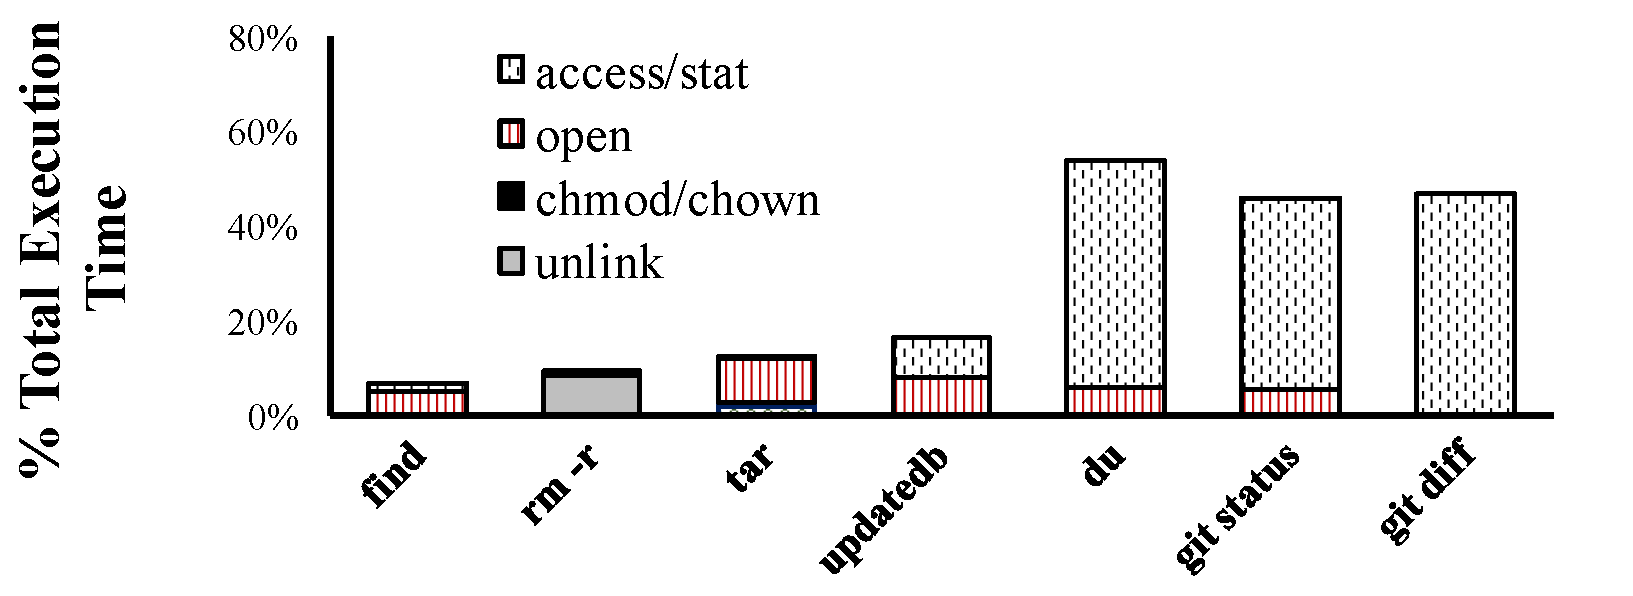
\includegraphics[width=5in]{dcache/plots/syscall-percentage.pdf} \\
\caption[Fraction of execution time on path-based system calls.]
{Fraction of execution time in several common utilities spent
executing path-based system calls with a warm cache, as measured with ftrace.}
\label{fig:dcache:lookup-frac}
%\vspace{-10pt}
\end{figure}

%\fixmedp{Please check these \% against time.  I think git diff is too high.  git status seems ok.}

Directory caches are essential for good application performance.
%Unix was designed such that ``(almost) everything is a file'',
%thus even accesses to in-memory file systems, device files, FIFOs and domain sockets
%first pass through the directory cache.
%In other words, 
Many common system calls must operate on file paths,
which require a directory cache lookup.
For instance, between 10--20\% of all system calls in the iBench system call traces do a path lookup~\citep{filenotafile}. 
Figure~\ref{fig:dcache:lookup-frac} lists the fraction of total execution time
%, as well as system time, 
several common command-line applications spend executing path-based system calls
(more details on these applications and the test machine in \S\ref{sec:dcache:eval}).
We note that these system calls include work other than path lookup,
and that these numbers include some instrumentation overhead;
% are coarse measurements that include  and work than path lookup;
%, and includes some time 
%for synchronous I/O (e.g., during {\tt rename}) as well as non-path tasks (e.g., creating 
%a file handle as part of {\tt open});
nonetheless, in all cases except {\tt rm},
the system call times and counts are dominated by
{\tt stat} and {\tt open}, for which 
%can be serviced from cache and for which 
path lookup is a significant component of execution time.
For these applications, path-based system calls account for 6--54\% of total execution time.
%and 25--77\% of system time.  
This implies that
lowering path lookup latency is
 one of the  biggest 
opportunities for a kernel to improve these applications' execution time.




\begin{figure}[t!]
\centering
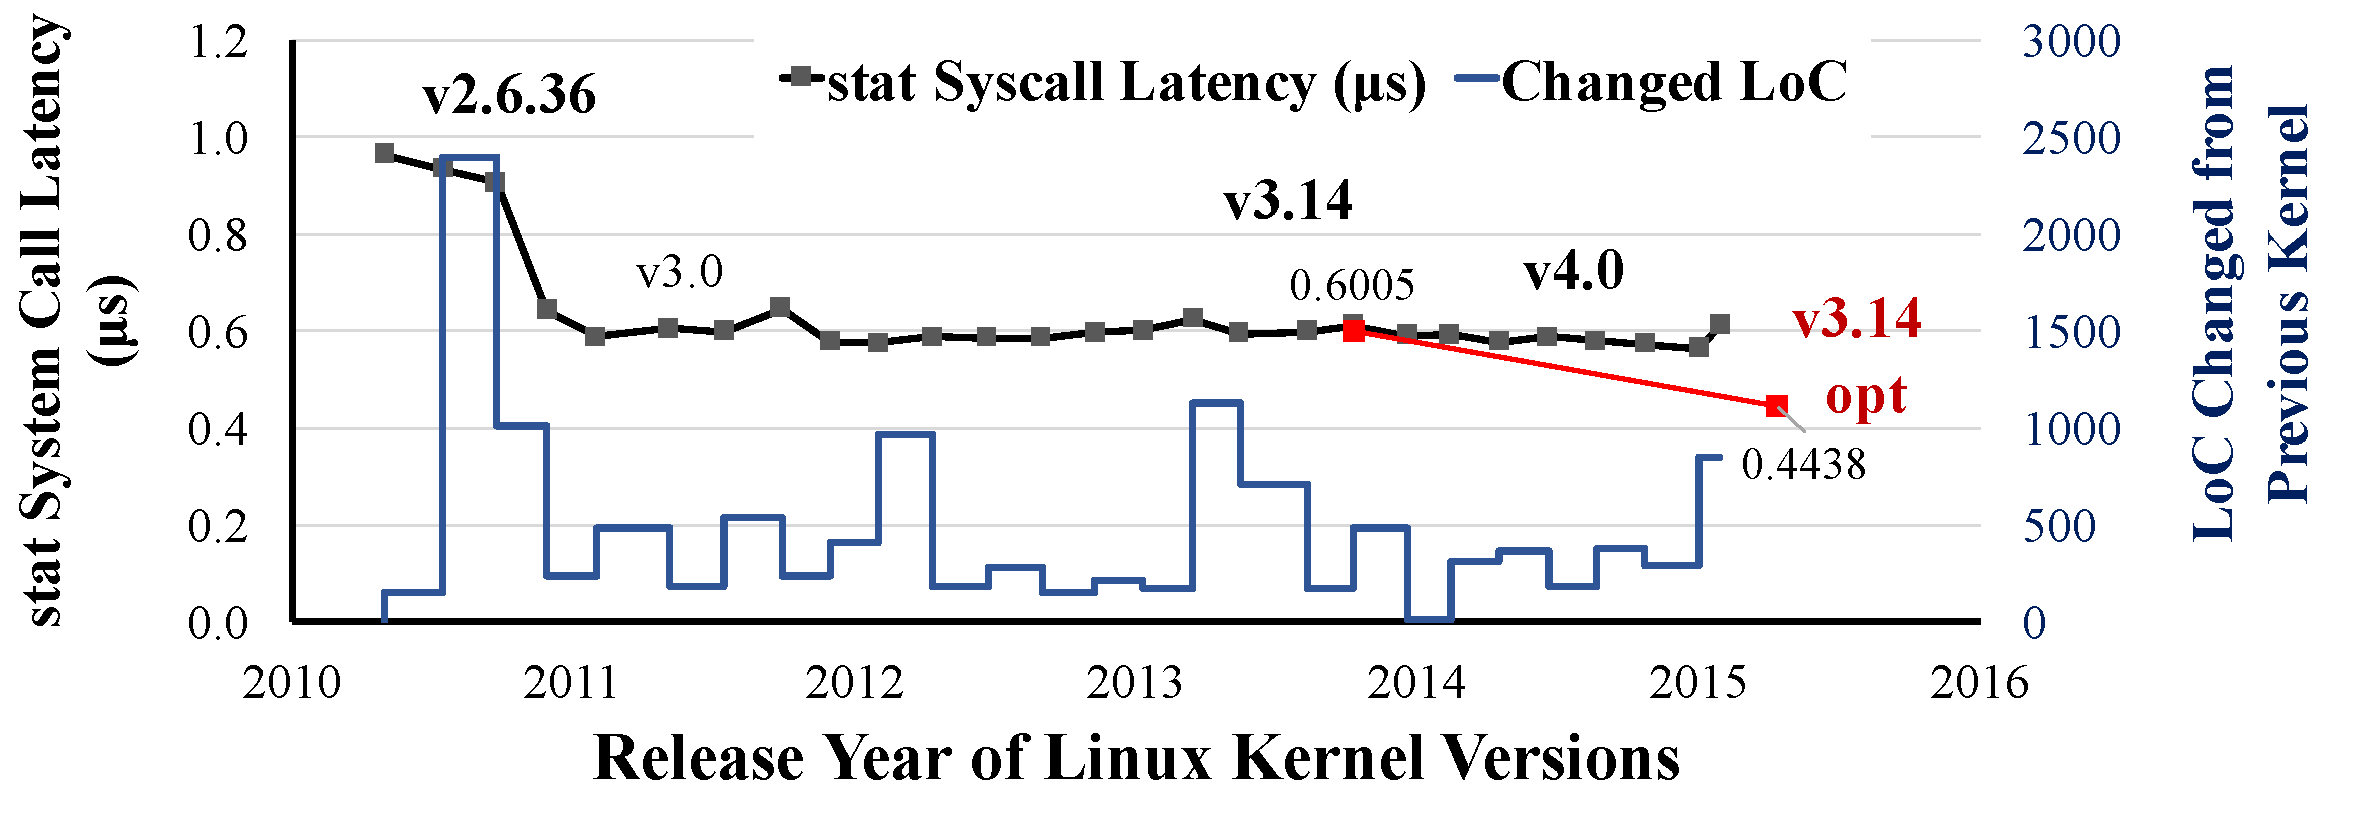
\includegraphics[width=6in]{dcache/plots/latency-by-version.pdf}
\footnotesize
\caption[Lantecy of {\tt stat} system call over years.]
{Latency of {\tt stat} system call with a long path {\tt XXX/YYY/ZZZ/AAA/BBB/CCC/DDD/FFF} on Linux over four years (lower is better), as well as the churn within the directory cache code (all insertions in {\tt dcache.c}, {\tt dcache.h}, {\tt namei.c}, {\tt namei.h} and {\tt namespace.c}). 
%Our optimizations significantly improve performance that has otherwise plateaued, despite significant ongoing developer effort.  
Our optimized \linuxver{} kernel 
further reduces {\tt stat} system call latency by \statspeedup{}\%.}
%\vspace{-15pt}
\label{fig:dcache:by-version}
\end{figure}


%\fixmedp{Add more evidence of lookup importance here: For instance, fraction of lookup time in file-related syscalls, or total lookup time in applications bound on file lookup latency.  }
Unfortunately, even directory cache hits are costly---0.3--1.1 \us{} for a {\tt stat} on our test Linux system, compared to only .04 $\mu$s for a {\tt getppid} and 0.3 \us{} for a 4 KB {\tt pread}. 
%\fixmetsai{Don, check this, I think read will be a better example, getppid is too trivial.}
This issue is taken particularly seriously in the Linux kernel community, which has 
made substantial revisions and increasingly elaborate optimizations to reduce the hit cost
of its directory cache, such as removing locks from the read path or replacing lock ordering with deadlock avoidance in a retry loop~\citep{corbet09jls,dcache-rcu}.
Figure~\ref{fig:dcache:by-version} plots directory cache hit latency against  lines of directory cache code changed 
over several versions of Linux, using a path-to-inode lookup \microbench{} on the test system described
in \S~\ref{sec:dcache:eval}.
These efforts have improved hit latency by 47\% from 2011 to 2013, but have plateaued
for the last three years.
%\fixmedp{if time, filter irrelevant changes from code deltas}
%at the cost of substantial developer effort.
%This latency appears to have plateaued 

The root of the problem is that the POSIX path permission semantics
seemingly require work that is linear in the number of path components,
and severely limit the kernel developer's implementation options.
%The root of this problem is that current directory cache
%designs reflect a straightforward implementation of the POSIX specification,
%which would seemingly require work that is linear in the number of path components.
For instance, in order to open file {\tt /\fnone{}/\fntwo{}/\fnthree{}} 
%for reading, 
one must have search permission
to parent directories {\tt /}, {\tt /\fnone{}}, and {\tt /\fnone{}/\fntwo{}},
as well as permission to access file {\tt \fnthree{}}.
The Linux implementation %of this specification is straightforward, 
simply walks the directory
tree top-down to check permissions.  
Unfortunately, when the critical path is dominated by 
walking a pointer-based data structure, 
including memory barriers on some architectures for multi-core consistency, 
modern CPUs end up stalling on hard-to-prefetch loads.
Moreover, because so many Linux features are built around this behavior, such as Linux Security Modules (LSMs)~\citep{wright+lsm},
namespaces, and mount aliases, it is not clear that any data-structural enhancements
are possible without breaking backward-compatibility with other Linux kernel features.
A priori, it is not obvious that a faster lookup algorithm, such as a single hash table lookup, 
can meet these API specifications and kernel-internal requirements; to our knowledge,
no one has tried previously.

%This paper proposes a decomposition of the directory cache, which allows
%most lookup operations to execute with a single hash table lookup (\S\ref{sec:dcache:dcache}),
%as well as optimizations to reduce the miss rate based on information that is {\em already in the cache}, but not used effectively (\S\ref{sec:dcache:readdir}).
%Our design maintains compatibility (\S\ref{sec:dcache:generalize}) through 
%several essential insights, including 
%how to separate the indexing of paths from checking parent permissions,
%and how to effectively and safely memoize the results of access control checks.


%% This paper proposes several new ways to organize a directory cache, which can yield 
%% substantial performance improvements over the current state of the art.
%% %This paper demonstrates that, despite this developer effort, there is still a substantial 
%% %missed opportunity hiding behind historical, intuitive, but not fundamental design choices.
%% Most of the Linux directory cache design reflects a straightforward implementation of the POSIX 
%% specification. %, with a division of labor that is suitable for mainstream file systems.

%This paper presents an alternative directory cache organization, which 
%improves performance by separating logical tasks, such as separating path indexing from permission checking; yet the design is sufficient to retain compatibility with POSIX.
%In the case of path lookup, 
%this paper demonstrates how 
%a per-component tree walk can be replaced with a single hash table lookup (\S\ref{sec:dcache:dcache}).
% without violating POSIX compliance.

%Our optimizations improve the performance of frequent lookup operations, but 
%introduce several costs, described in \S\ref{sec:dcache:dcache} and measured in \S\ref{sec:dcache:eval},
%which  we believe are acceptable and a net improvement for applications.
%First, these optimizations slow down infrequent modifications to the directory hierarchy, such as {\tt rename}, {\tt chmod},
% and {\tt chown} of a directory. 
%However, these slower operations
%account for less than .01\% of the system calls in the iBench traces~\citep{filenotafile}.
%Second,  the memory overheads of the dcache are increased.
%%(45\% per \dentry{}, as well as some  in our prototype).
%%(\fixmedp{XX MB} in our tests).  
%Third, lookup has a 
%probability of error from signature collisions that can be adjusted to be negligible
%%($2^{-141}$ in our configuration), 
%and within acceptable thresholds widely used by data deduplication systems~\citep{Debnath:2010:CSU:1855840.1855856, Srinivasan:2012:ILI:2208461.2208485, Quinlan:2002:VNA:645371.651321, Zhu:2008:ADB:1364813.1364831}.
%%, as well as how to remove
%%all memory barriers from the lookup path (\S\ref{sec:dcache:update}).
%In the micro-benchmark of Figure~\ref{fig:dcache:by-version}, our directory cache 
%optimizations improve lookup latency by 
%%revisions improve latency of accessing a long path
%%by 
%\statspeedup{}\% over unmodified Linux.
%%Our design addresses other missed
%%opportunities, such as identifying new opportunities to reduce the miss rate
%%through caching directory completeness.
%%\fixmedp{Do we want to highlight LoC?  3K is more than anything in the graph} \fixmetsai{Probably just mention in the evaluation. It's a metric that we should provide, but it's not awfully interesting.}
%%The total lines of code changed are fewer than 3,000 out of \fixmedp{XX}.
%%\fixmedp{Can we get 
%%, yet changes fewer than 3,000 lines of code.

%% SOSP cut - kind of long-winded
\begin{comment}
This paper rethinks current Linux directory cache design choices in light of the following goals:
\begin{compactitem}
\item {\bf Minimize the cost of a cache hit.} (\S\ref{sec:dcache:dcache}).
This means maximizing the benefit of temporal locality for frequent operations,
while pushing extra work of consistency maintenance onto less frequent, already-expensive operations.
%such as handling cache miss or updating massive metadata,
%in order to improve very frequent operations.
\item {\bf Maintain legacy compatibility.} (\S\ref{sec:dcache:generalize}).  Unix path semantics are complex, required by applications, file systems, and security modules, frustrating otherwise straightforward optimizations.  However tempting it may be to redesign path behavior to facilitate caching, path operations must exhibit the same behavior, with lower latency.
\item {\bf Never miss the same request twice in quick succession.} (\S\ref{sec:dcache:readdir}).  A number of less-frequent operations, such as reading a directory or secure temporary file creation, always miss in the cache {\em even if enough information is in cache to satisfy the operation.}  
%Of course, infrequent accesses should still be subject to a cache replacement policy, such as LRU.
\end{compactitem}
%Although directory caches must implement more complex semantics than a hardware memory cache,
%these principles should seem familiar to the reader with a basic architecture background.
%sadly, the Linux directory cache design violates all three.
\end{comment}

%This paper introduces several techniques to improve the performance of a directory cache,
%This paper explains several practical directory cache optimizations,
This paper demonstrates that these techniques improve performance for applications that use the directory cache heavily,
and the harm is minimal to applications that do not benefit.
%and that the worst case \microbench{} is only 12\% slower within \fixmedp{XX}\% of unmodified Linux.
%Each optimization we describe improves performance in isolation, and all can be combined.
%These optimizations change very few lines of code, and are backward-compatible with 
%legacy applications.  
%These changes are encapsulated in the VFS---individual file systems do not have to change their code.
%This paper describes a  prototype of these improvements implemented in Linux \linuxver{}.
%\S~\ref{sec:dcache:background} explains that the directory cache structure of Mac OS X, FreeBSD, and Solaris 
%are sufficiently similar that these principles should generalize.
%we compare and contrast Linux's directory cache
%with Mac OS X, FreeBSD, and Solaris in \S\ref{sec:dcache:background}, and explain inline how each
%optimization could be generalized to these other OS kernels.





%% \item {\bf Modularization and stackability}:
%% Any changes or optimizations must be implemented as modules inside Linux's VFS,
%% and can be stacked on top of the original design or any future optimizations. 
%% \item {\bf Backward compatibility}:
%% Any changes or optimizations must maintain least requirement of modifying any
%% file systems.
%% \item {\bf Generalization to other OSes}: Any changes or optimizations must be portable to other OSes with reasonable effort and change of design.




%% \dcache{} is proven to be effective on improving storage performance.
%% Experiments shows that,
%% in a Linux 3.x kernel, a \dcache{} with a xxx\% hit rate can speed up
%% metadata lookup and fetching time by xxx times.
%% \fixmetsai{experiment result, Linux version, and fs specs here}
%% However, we observed that Linux maintainers have made
%% constant and non-trivial efforts to improve \dcache{} in the Linux kernel.
%% We studied all \dcache{}-related source files in the Linux kernel Git repository,
%% and discovered that maintainers have committed
%% on average xxx revisions per source files.

%% We tested metadata lookup time on primary \dcache{}-related revisions.
%% Most changes on \dcache{} system only create xxx\%-xxx\% speed-up
%% than their predecessor.
%% \fixmetsai{result and graph here}.
%% Moreover, improvement to \dcache{} is still work-in-progress
%% for Linux maintainers.
%% \fixmetsai{reference to threads for latest dcache discussions}. 
%% All the evidences show that,
%% despite of significant reduction of storage operations,
%% efficiency of \dcache{} system internally still remains as a concern.

%% We argue that the design of \dcache{} needs to be carefully re-examined,
%% to fundamentally identify any missed opportunities that
%% improve value of \dcache{}.
%% At a high level, most optimization works for \dcache{} are focused on
%% improving ``how to cache'',
%% but we want to also lay eyes on ``what to cache'',
%% to ensure any valuable information returned from file systems
%% be captured by \dcache{} system.

%The contributions of this paper are as follows:
%\begin{compactitem}
%\item A performance analysis of the costs of path lookup and the opportunities
%to improve cache hit latency.
%\item A directory cache design that improves path lookup latency with a combination of techniques, including:
%  \begin{compactitem}
%  \item Indexing the directory cache by full path, reducing average-case lookup from linear to constant in the number of path components.
%  \item A Prefix Check Cache (PCC) that separates permission checking from path caching.  The PCC memoizes permission checks, and is compatible with LSMs~\citep{wright+lsm}.
%  \item Reducing the cost of checking for hash bucket collisions with path signatures.
%  \end{compactitem}
%\item Identifying opportunities to leverage metadata the kernel already has to reduce miss rates, such as tracking whether a directory is completely in cache.
%\item Carefully addressing numerous, subtle edge cases that would frustrate rote application of these techniques, such as integration with symbolic links and Linux namespaces.
%\item A thorough evaluation of these optimizations.  For instance, our optimizations improve throughput
%of the Dovecot IMAP server by up to \dovecotspeedup\% and latency of 
%updatedb by up to \updatedbspeedup{}\%.
%%git version control system by up to 25\%.
%
%\end{compactitem}

%\section{Background}
\label{sec:background}

This section summarizes \sgx{},
and current design points for running or porting applications on \sgx{}.
%and the legacy frameworks of porting 
%including \haven{}~\cite{baumann14haven}, \scone{}~\cite{osdi16scone}, and Panoply~\cite{shinde17panoply}. 


\subsection{Software Guard Extensions (SGX)}
\label{sec:background:sgx}

%\begin{figure}[t!]
%\centering
%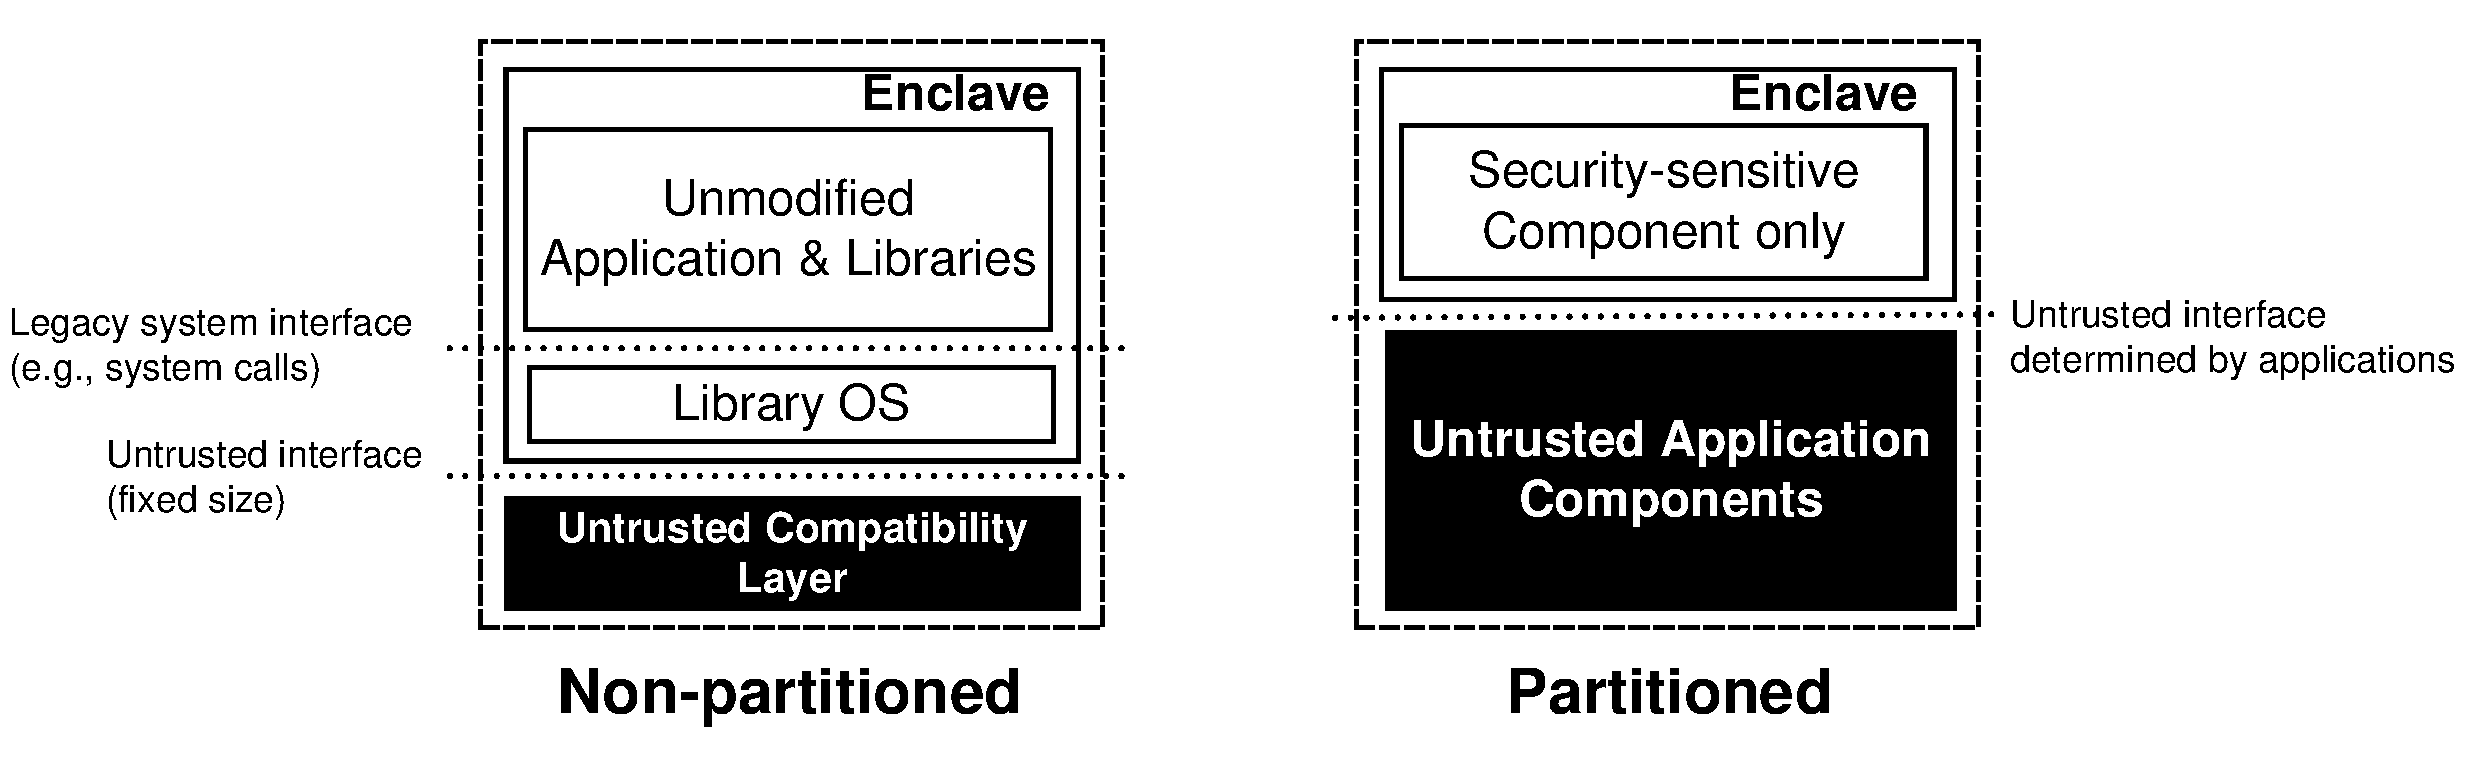
\includegraphics[width=\linewidth]{figures/libosvssdk.pdf}
%\footnotesize
%\vspace{-0.3in}
%\caption{
%Comparison between libOS-based model (e.g., \haven{} and \graphenesgx{})
%and SDK-based (SDK for \sgx{}) model for migrating applications in enclaves.
%Green (light) boxes are trusted components and red (dark) boxes are untrusted.
%The libOS-based model often yields a larger TCB in the enclave,
%while the SDK-based model requires developers to be responsible of
%securing the enclave on the untrusted interface.
%}
%\label{fig:libosvssdk}
%\end{figure}

The primary SGX abstraction is an \emph{enclave}: an isolated execution environment within the virtual address space of a process.
The code and data in enclave memory do not leave the CPU
package unencrypted; when memory contents are read back into cache,
the CPU decrypts the contents, and checks the integrity of cache lines and the virtual-to-physical mapping.
SGX also cryptographically measures the integrity of enclaves at start-up, and 
provide attestation to remote systems or other enclaves.
%Remote entities can identify the owners of enclaves by distinguishing the cryptographic measurements
%generated with different signing keys.

%%% \sgx{} is a new feature on the 6th-genaration \intel{} CPUs.
%%% it contains a set of new x86/64 instructions, to initiate, destroy, and attest isolated execution environments (i.e., enclaves) in the address space of applications.
%%% When \sgx{} loads an application in an enclave,
%%% the code and data of the application will remain encrypted in the main memory,
%%% forbidding any mean to eavesdrop the application secrets.
%is a set of new x86/x64 instructions introduced
%to the latest \intel{} CPUs,
%to bootstrap an isolated execution environment
%inside applications' virtual memory address space.
%\sgx{} creates a memory region
%(generally referred as {\bf enclave}), storing both the code and data of the isolated execution,
%which stays encrypted in DRAMs and only the CPU is capable of encryption and decryption.
%The CPU derives the encryption key
%from the cryptographic measurement of the initial state of enclave memory,
%to allow remote entities to verify the soundness of execution and establish the trust
%needed for provisioning sensitive data.

\sgx{} enables a threat model where one only trusts the \intel{} CPUs and the 
code running in the enclave(s).
%whereas the rest of application, system software, off-CPU-package hardware devices and providers are untrusted. 
\sgx{} protects applications from three different types of attacks on the same host, which are summarized in Figure~\ref{fig:sgx-threats}: untrusted application code inside the same process but outside the enclave; operating systems, hypervisors, and other system software;
%\fixme{added Mona's suggestion}
other applications on the same host; and off-chip hardware.
A SGX enclave can also trust a remote service or enclave, and be trusted after inter-platform attestation~\cite{sgx-attestation}.




%%% \begin{compactenum}

%%% \item {\bf Inside process memory:}
%%% \sgx{} partitions the application process into two privilege levels, as the trusted part (in enclaves) which can access the whole process memory, and the untrusted part (outside enclaves) forbidden to access enclave memory.
%%% %the privileged part (in the  enclave region) can access all process memory,
%%% %while the unprivileged part (outside the enclave region) is limited to access only data that are not isolated by \sgx{}.

%%% \item {\bf From hosting OSes or hypervisors:}
%%% \sgx{} assumes that OSes and hypervisors can be compromised by either exploiting system vulnerabilities
%%% or malicious system software installed by administrators.
%%% Both types of compromise are legitimate threats to modern OSes, due to complexity of modern OSes and usage of public facilities like clouds.

%%% %Operating systems or hypervisors
%%% %that are either compromised by rootkits
%%% %or deliberately modified by the host providers.
%%% %An attacking host can access the raw data in DRAMs, or remap the
%%% %physical pages to other contexts.

%%% \item {\bf Physically from the hardware:}
%%% One type of attacks that cannot be defended by software-based solutions~\cite{flicker, criswell2014virtualghost}
%%% is from the attackers who have physical access to the hosts.
%%% \sgx{} can resist attacks on the host hardware
%%% including hacking peripheral devices like ethernet cards and connectors~\cite{hudson15thunderstrike}, tapping into buses, or eavesdroping DRAM data using Cold-boot attack~\cite{halderman09coldboot}.


%%% \end{compactenum}


%%% \sgx{} protects an application against unpredictable threats from both local and remote hosts.
%%% \sgx{} establishes a trusted path
%%% from one enclave to another,
%%% providing end-to-end protection to both enclaves to
%%% exchange data with confidentiality and integrity.
%%% %, processing the data and returning the computation results with end-to-end protection.
%%% We can further divide up the protection using \sgx{} into three elements:
%The use cases of \sgx{} mostly involve the process that an enclave
%retrieves a signed attestation from the processor,
%to exchange provisioning of critical information from remote servers.
%The purpose of such process is equivalent to
%expanding the trusted execution
%from remote servers
%to untrusted hosts,
%to harness resources such as CPU cycles and DRAMs.

%%% \begin{compactenum}

%%% \item {\bf Isolated execution:}
%%% \sgx{} guarantees the execution initiated in an enclave
%%% to be isolated from any part of the system except the enclave itself.
%%% %any part of the system except the enclave itself can access the execution state. 
%%% Achieved by the secrecy of encryption keys in \intel{} CPUs.

%%% \item {\bf Attestation of integrity:}
%%% Remote entities with a \sgx{}-enabled CPU can verify the integrity of an enclave, using the \intel{} Attestation Services (ISV)~\cite{isv}.
%%% %for its integrity of running the exact code that it is given.
%%% Achieved by the uniqueness of CPU keys to sign the cryptographic measurement of enclaves.

%%% \item {\bf Authentication:}
%%% Remote entities can identify the owners of enclaves by distinguishing the cryptographic measurements generated with different signing keys.


%%% %explicitly launched for processing the specific tasks, regardless of the identicality of execution.
%%% %That is, two mutually distrusting users can launch the same execution in  separate enclaves, yet be able to distinguish by the measurements as MACs (Message Authentication Code) signed by the users' private keys.

%%% \end{compactenum}


%One must note that \sgx{} only promises the integrity of application binaries
%initially loaded in enclaves.
%The gap between integrity of binaries and complete security has to be filled
%by ones who develop and approve the applications.
%More specifically, the clients are responsible of
%testing whether the applications contain any vulnerabilities
%that lead to information leak.
%To minimize the risk of leaving any flaws in the applications unintentionally,
%developers often tend to cut down the trusted computing base (TCB)
%of the applications. With smaller TCB, clients who launched the enclaves
%can more easily reason about the thoroughness of securing the execution.

%To achieve smaller TCB, the software development kit of \sgx{}
%intends to encourage developers to partition the applications and
%keep only security sensitive components in the enclaves.
%Such an intention is exactly contradicted by the trust model of \haven{},
%which must trust the loaded application as a whole.
%Except for the cases in which the whole applications must be secured,
%\haven{} actually downgrades the trustworthiness of enclaves.
%Figure~\ref{fig:libosvssdk} shows the comparison of the two models.


%%% By synthesizing and streamlining these three elements (i.e., isolation, attestation and authentication),
%%% \sgx{} provides a promising build block to securing applications
%%% from unpreditable security threats.

%developing applications
%that are resistant to unpreditable, unavoidable threats.
%Users expect \sgx{} to build up a wall for protecting the sensitive data, even against a catastrophic scenario like a complete takeover of the infrastructure.  

%\fixmedp{Explain how to read the figures in the captions. What do colors and shading mean?}
%
%\fixme{Disabled the whole discussion about SDK. dp: ok with me, but probably drop from figure} 
\begin{comment}
\subsection{The legacy framework (The \sdk{})}

{\bf Intel's \sgx{} SDK} (software development kit) for Linux~\cite{intel-sgx-sdk} is the official framework
for programming \sgx{} execution within Linux applications.
\sdk{} includes the components of two phases:
a {\bf compile-time utility} to generate a valid executable for running inside enclave,
and a {\bf run-time framework} to trigger the hardware-enforced isolated execution.
The two-phased design is based on the assumption that compilation of applications
is controlled by trusted, security experts,
to retain the trustworthiness of isolation model when running on untrusted OSes.


The work flow of \sgx{} programming using \sdk{} is as follows:
\begin{compactenum}
\item At the build-time (on trusted hosts), developers create a self-contained, static executable as the initial code and data after enclave creation.
We refer the executable as an ``enclave image''.
The enclave image is statically links with the enclave infrastructure, which provides enclave APIs (e.g., retrieving attestation) and a extremely small set of POSIX functions (e.g., {\tt memset()}).
After linking, the compile-time utility signs the executable and inserts the enclave signature structure
({\tt SIGSTRUCT}) in the application code.
\item At the execution-time (on untrusted hosts), the enclave image is taken by the framework. The user-space driver then requests enclave creation with the kernel driver, through {\tt ioctl()} to a pseudo-device {\tt /dev/isgx}.
The kernel driver creates and initializes an enclave using the authenticated signature structure,
and a token exchanged from an architectural enclave, {\tt AESMD}, for ensuring the validity of enclave. 
\end{compactenum}





%During the compile time,
%the developers create a self-contained, static binary, as the initial image of an run-time enclave (an ``enclave image'').
%\sdk{} provides the infrastructural libraries (libsgx) for static linking, which contain enclave APIs and few POSIX functions.
%A signing tool of \sdk{} will generates a valid enclave signature
%derived from the enclave image.
%Both the static linking and signing must happen on a trusted, development machine.


%After generating the enclave image, developers then ship it with the rest of application,
%to untrusted hosts (\sgx{}-enabled)
%where the \sdk{} run-time framework is installed.
%The run-time framework provides both kernel and user-space drivers,
%to interface \sgx{} hardware using the new x86 instructions (e.g., {\tt ECREATE}, {\tt EADD}, {\tt EENTER}).
%The framework also includes an architectural enclave (AESM), for validating the enclave attributes (and generating a run-time token),
%and a kernel EPC (enclave page cache) driver that manages paging for all running enclaves.



% includes both compile-time and run-time components:
%for the compile time, the SDK provides all the infrastructure libraries,
%which the applications statically link with,
%and a signing tool that generates the enclave signatures for hardware validation.
%The run-time framework then takes the signed enclave binaries,
%and uses the kernel and user-space drivers to initiate the isolated execution in enclaves.



\sdk{} centers the whole programming model based on the concept of partitioning an application,
and isolating only minimum application code in enclaves.
The partitioning minimizes the risk of compromising the enclaves,
due to smaller trusted computing base (TCB) and less opportunity of omitting security glitches.
With this model,
developers are expected
to identify the part of an application that performs the sensitive operations,
and define an validated interface to
the sensitive part and rest of the application.
\sdk{} encourages partitioning by reducing the difficulty of defining and accessing the interface---a language tool automatically generates the interface code with extra argument-sanitizing code.
The generated interface code essentially filters input and output of the enclave,
and prevents randomly copying memory across the enclave boundary, leaking or corrupting internal data.


%The Intel SDK has its limitations. The infrastructure of the SDK provides APIs in enclaves for accessing SGX features (e.g., attestation), as well as a small set of POSIX APIs
%(\roughly{}10 functions, such as {\tt printf} and {\tt memset}).


Despite that \sdk{} attempts to alleviate the difficulty of partitioning for SGX,
porting a piece of application code that is sophisticated and interactive to the rest of application
is still a significant cost to pay.
In general, developers want to find a reasonable granularity of partitioning---a ``sweet spot'' that partitions the application code neither too small nor too large, 
to nicely balance between frequency of enclave exits and risk of introducing incompatible code.
For an application written in C/C++, partitioning is cumbersome especially if the application is poorly modularized.


Unfortunately, the limited POSIX support in the \sdk{} infrastructure really strikes
the opportunity of fine-grained partitioning.
The lack of POSIX APIs in the infrastructure is fundamental, due to the restriction
on OS interaction from the enclaves.
The missing APIs encapsulates system calls, which can expose the enclave to some risky OS interaction model, such as {\bf Iago Attacks}~\cite{checkoway13iago}.

%In conclusion, this work targets on completing the API support, either at POSIX level or system calls,
%while retaining the isolation model.
%The platform can assist developers to refocus on partitioning applications for minimizing the risks.

\end{comment}

\subsection{SGX Software Design Space}

This subsection summarizes the principal design choices facing any 
framework for running applications on SGX.  We explain the decisions in
recent systems for SGX applications, and the trade-offs in this space.

\begin{figure}[t!]
\centering
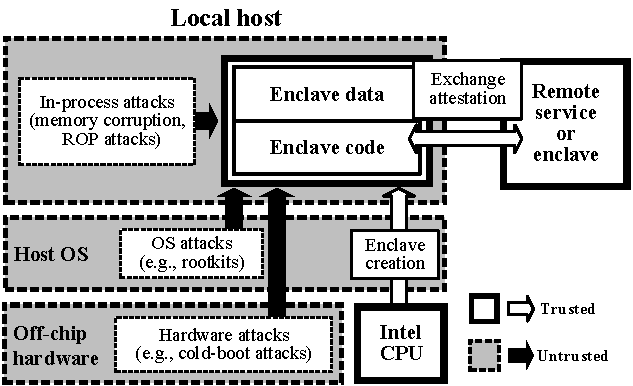
\includegraphics[width=.5\linewidth]{sgx.pdf}
\caption{The threat model of \sgx{}. \sgx{} protects applications
from three types of attacks:
in-process attacks from outside of the enclave,
attacks from OS or hypervisor, and attacks from off-chip hardware.}
% Red (dark) boxes are untrusted components and green (light) boxes are trusted.}
%For each enclave, \sgx{} establishes the chain of trust from the \intel{} CPU.
%Enclaves across physical machines or even infrastructures can remotely attest the integrity of execution, using the signatures generated and signed by the CPU.
%Green (light) boxes and arrows represent the trusted components and operations, and red (dark) boxes and arrows represent the otherwise.
\label{fig:sgx-threats}
\end{figure}

\paragraph{How much functionality to pull into the enclave?}
At one extreme, a library OS like Haven~\cite{baumann14haven} pulls most
of the application-supporting code of the OS into the enclave.
On the other extreme, thin ``shim'' layers, like SCONE~\cite{osdi16scone} and Panoply~\cite{shinde17panoply} 
wrap an API layer such as the system call table.
Pulling more code into the enclave increases the size of the TCB,
but can reduce the size and complexity of the interface, and attack surface, 
between the enclave
and the untrusted OS.

The impact of this choice on performance
largely depends on two issues. First, entering or exiting the enclave 
is expensive; if the division of labor reduces enclave border crossings, 
it will improve performance.
The second is the size of the Enclave Page Cache (EPC),
limited to 128MB on version 1 of SGX.
If a large supporting framework tips the application's working set size
past this mark, the enclave will incur expensive swapping.


\paragraph{Shielding complexity.}
SGX hardware can isolate an application from an untrusted OS, but 
SGX alone can't protect an application that  requires
functionality from the OS.  {\em Iago attacks}~\cite{checkoway13iago}
are semantic attacks from the untrusted OS against the application, where an unchecked system call return 
value or effect compromises the application.
Iago attacks can be subtle and hard to comprehensively detect, at least with the current
POSIX or Linux system call table interfaces.

Thus, any SGX framework must provide some {\em shielding} support, to 
validate or reject inputs from the untrusted OS.  
The complexity of shielding is directly related to the interface complexity:
inasmuch as a library OS or shim can reduce the size or complexity of the 
enclave API, 
the risks of a successful Iago attack are reduced.

\paragraph{Application code complexity.}
Common example applications for SGX in the literature 
amount to a simple network service running a TLS
library in the enclave, putting minimal demands on a shim layer. 
Even modestly complex applications, such as the R runtime and a simple
analytics package, require dozens of system calls providing wide-ranging functionality, 
including \syscall{fork} and \syscall{execve}.
For these applications, the options for the user or developer become: 
(1) modifying the application to require less of the runtime; (2) opening and shielding more 
interfaces to the untrusted OS; (3) pulling more functionality into a shim or a library OS.
The goal of this paper is to provide an efficient baseline, based on (3),
so that users can quickly run applications on SGX, and developers can 
explore (1) or (2) at their leisure.

\paragraph{Application partitioning.} An application can have multiple
enclaves, or put less important functionality outside of the enclave.
For instance, a web server can keep cryptographic keys in an enclave,
but still allow client requests to be serviced outside of the enclave.
Similarly, a privilege-separated or multi-principal application might create a separate enclave for
each privilege level.

This level of analysis is application-specific, and beyond the focus of this paper.
%which is on running unmodified applications in enclaves.
However, partitioning a complex application into multiple enclaves
can be good for security. In support of this goal,
\graphenesgx{} can run smaller pieces of code, such as a library, in an enclave, as well as
coordinate shared state across enclaves.

%* Partitioned vs. unpartitioned app?

%** Right choice depends a lot on whether the app has multiple principals or security concerns.

\begin{comment}
\fixmedp{Did a first cut at 2.2; needs to integrate the figure (or drop it).  I didn't know what to write for 2.3 yet.  I left the old text below for now (if there is anything you really want to save), but it needs to go away}

\subsection{Open Challenges}

\fixmedp{Here, I would give a taste of some of the issues we solve and why they are hard, like dynamic loading (and maybe fork or IPC).  Keep it short, a few paragraphs.}
\end{comment}

%\begin{figure}[t!]
%\centering
%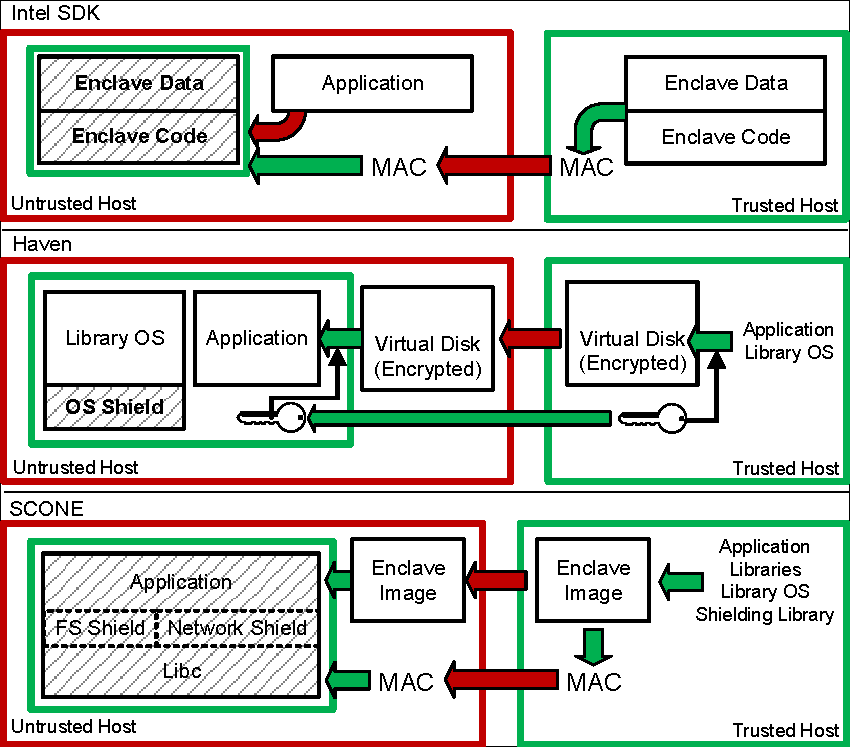
\includegraphics[width=\linewidth]{figures/sdkvslibos.pdf}
%\caption{Comparison of the code integrity model among different \sgx{} frameworks, including the \sdk{}, \haven{} and \scone{}.}
%%Green (light) boxes and arrows represent the trusted components
%%and operations, and red (dark) boxes and arrows represent the otherwise.
%%Patterned blocks represent the code and data included in the initial measurements of the enclaves.}
%\label{fig:sdkvslibos}
%\end{figure}


\begin{comment}
\subsection{\sgx{} shielding systems}
\label{sec:background:shielding-systems}




The current \sgx{} shielding systems, such as \haven{}~\cite{baumann14haven}, \scone{}~\cite{osdi16scone}, and Panoply~\cite{shinde17panoply}, enforce end-to-end isolation to
legacy applications without partitioning.
A \sgx{} shielding system preserves the trusted computing base (TCB)
of an application, and further increases it with a shielding layer to defend against the untrusted OSes.
By avoiding application partitioning,
%model of quarantining an unmodified, COTS application in an \sgx{} enclave.
a shielding system minimizes the effort of reprogramming the applications for \sgx{} execution, often with recompilation or packaging the binaries in an encrypted enclave.
%to merely recompiling or packaging the application code before signing it off for enclave execution.
%These \libos{}es internalize OS features into the enclave, to maintain a fixed-size,
%narrow interface to the untrusted host OSes.
%Porting applications using a \sgx{} \libos{} is vastly different from the programming model of \sdk{}---no programming effort is needed when porting with a \sgx{} \libos{}, and applications are isolated without partitioning.
In the following paragraphs, we compare the current shielding systems with the \graphenesgx{} approach.

\haven{}~\cite{baumann14haven} uses a \libos{} called \drawbridge{} in each enclave
to shield a single-process \emph{Windows} application from the untrusted host OS.
\haven{} absorbs the implementation of system APIs (i.e., Win32 APIs) from the host OS,
%\haven{} uses \drawbridge{}~\cite{porter11drawbridge} as the backbone of its enclave infrastructure, 
and exports a narrow enclave interface on which untrusted inputs are carefully filtered to defend against the Iago-type attacks.
Adding a \libos{} to each enclave causes a bloat of TCB---for \haven{}, the size of a \libos{} binary and shielding layer is \roughly{}200MB.
\haven{} has to establish the trust and integrity in all these binaries loaded into an enclave. Except that the shielding layer is a part of the enclave since its creation, \haven{} enforces the integrity of both the \libos{} and the isolated application,
by storing all binaries on an encrypted virtual disk and relying a remote, trusted server to provision the key for decryption.
\haven{} builds a trusted path from a remote server to local cloud machines,
to securely bootstrap application execution inside the enclaves.
%Other minor comparison between \haven{} and this work: the development and evaluation of \haven{}, at publication, is based on a simulated architecture.
%On the contrast, \graphenesgx{} is a released open-source platform, tested by many developers from institutes and corporations. \fixme{maybe bring up TCB?}



\scone{}~\cite{osdi16scone} isolates Linux micro-services in enclaves as a container-like environment.
After a brief attempt of building a \libos{} like \haven{},
\scone{} chooses a different approach of shielding the system API usage in applications, by designing shielding strategies based on each API.
\scone{} stacks the application on top of file-system and network shielding libraries, and extends a standard library C (musl~\cite{musl}) to securely exit the enclave for system calls.
Within the \sgx{}-aware Libc, \scone{} carefully filters the inputs from the host system calls, as the defend against known Iago attacks.
For instance, \scone{} ensures that pointers given to and returned by a host system call will point to addresses outside the enclave,
to prevent the host OS to manipulate pointers and cause memory corruption in the enclave.
\scone{} also authenticates or encrypts file or network streams
based on configurations given by the developers.


%The \libos{} implementation in \scone{} is based on musl~\cite{musl} and LKL (Linux kernel library)~\cite{lkl}.
%The design of a SCONE enclave (or Secure Container) has similarity
%with a basic block of \graphenesgx{}:
%they both validate input files based on cryptographic methods, and are fully configurable at a per-file basis.
%However, \graphenesgx{} supports a more complete set of Linux system APIs.
%The APIs that \graphenesgx{} especially contributes over \scone{} are the Linux multi-process APIs, including copy-on-write {\tt fork()}, {\tt exec()}, signals, and system V IPC (message queues and semaphores).

Panoply~\cite{shinde17panoply} further reduces the TCB of a shielding system over the SCONE approach, by excluding both a \libos{} and \libc{} from enclaves.
Instead, Panoply uses a shim layer shielding a portion of the POSIX API. The shim layer yields about 20 KLoC as its TCB (trusted computing base), which is much smaller than libc and/or a library OS.
% in other shielding systems.
As Panoply delegates the libc functions outside the enclave, its shim library defends the supported POSIX API,
including 91 {\em safe} functions and 163 {\em wild (unsafe)} functions.
Panoply also supports multi-process API including \fork{}, \exec{}, signaling, and sharing untrusted memory with inline encryption.
Compared to \graphenesgx{}, Panoply has made some different design decisions in supporting multi-process API,
including supporting fork by copying memory on-demand with statically determining memory access,
and using secured messaging for inter-process negotiating instead of coordinating over an encrypted RPC stream.




\subsection{Comparison and security implications}

\fixme{need to drop the SDK discussion, revisit the security claims, and discuss Iago attacks in details.}

Figure~\ref{fig:sdkvslibos} shows the comparison between \haven{}, \scone{}, Panoply, and \graphenesgx{}.
%The \sdk{} model uses a static MAC of the enclave code and data, given to the \sgx{} driver for bootstrapping the isolated execution.
The \haven{} model only initiates enclaves with the OS shield layer,
which unpacks the enclave binaries from a virtual disk---decrypted using a provisioned key.  
The \scone{} model extends the \sdk{} model---it statically links the application binaries with the shielding library, creating a static enclave image verifiable by its MAC. The \sdk{} and \scone{} model retain more flexibility in deploying and integrating \sgx{} enclaves by focusing on the code integrity rather than encryption.

The key concerns that affects users choosing among these solutions are {\bf trusted computing base (TCB) size} and {\bf attack surface}.
However, since all these solutions are based on different design decisions, assumption and requirements, the comparison of TCB size and attack surface is often imprecise and inconclusive.

\paragraph{TCB size.}
Most studies measure the TCB size of a system by the total LoC (lines of code) written for all the trusted components, or the size (in bytes) of all the trusted binaries.
The comparison of TCB size is only meaningful when two systems have comparable system features,
and are order-of-magnitude different in term of LoC or binary size.
For instance, the comparison of TCB size between \haven{} and \scone{} is never an apples-to-apples comparison.
The implemented system features and personalities
in these two systems are fundamentally different, and \haven{} supports a much larger fraction of Windows features than the fraction of Linux features supported by \scone{}.

We argue that the only occasion that the reduction of TCB size
can be convincingly demonstrated is when a design has partitioned a system into isolated components,
or removed unreachable execution paths.
For instance, the \sdk{} promotes application partitioning for \sgx{};
it requires additional partitioning effort but is effective for confining the TCB size.
By statically linking the application binaries
with the shielding layers and standard C library, \scone{} offers more opportunities in stripping the Libc and shield code of unused APIs, and thus reducing its TCB size.



\paragraph{Attack surface.}

Most studies estimate the severity of having an attack surface by the size of interface to the trusted and untrusted components.
The experience of \scone{} provides an important insight for estimating attack surface: the narrowness of interface is not proportional to the difficulty of defending against incoming attacks.
An interface overloaded with too many features or semantics can become a major source of vulnerabilities.

%\subsection{The \graphene{} Library OS}
%
%\graphene{}~\cite{tsai14graphene} introduces a \libos{} design that supports
%both single-process and multi-process Linux applications,
%but retains a narrow host interface (43 functions) as a vantage point for enforcing security isolation.
%The main contribution of \graphene{} is an distributed implementation of the POSIX namespace coordination,
%to support Linux multi-process abstractions across \libos{} instances.
%All the multi-process abstractions in \graphene{} is implemented using simple pipe-like RPC streams,
%without relying on any host memory sharing support.
%Based on this design, \graphene{} can easily isolate mutually untrusting applications,
%by blocking the RPC streams between unrelated applications.
%
%
%
%The design decisions made by \graphene{} are important keys to the \graphenesgx{} framework.
%First, the host interface contains mostly internal abstractions, and three external ones including files, network connections, and RPC streams.
%The simplicity of the host interface facilitates shielding the \libos{}
%from risky OS interaction.
%Moreover, \graphene{} implements multi-process abstractions across instances without memory sharing.
%\graphenesgx{} can rely on the distributed POSIX implementation
%to support multi-process applications across multiple enclaves, by coordination over validated RPC streams.


\end{comment}




\papersection{Background and Motivation}
\label{sec:background}

%\fixmets{1.5 page}

This section discusses the security features of  \sgx{}, and the challenges faced by developers that
intend to use \sgx{} for partitioning \java{} applications.
%the key challenges developers face when trying to manually partition applications using a technology such as \sgx{}.
%discuss the programming models and threats to security of \sgx{} enclaves.

\begin{figure}[t!]
\centering
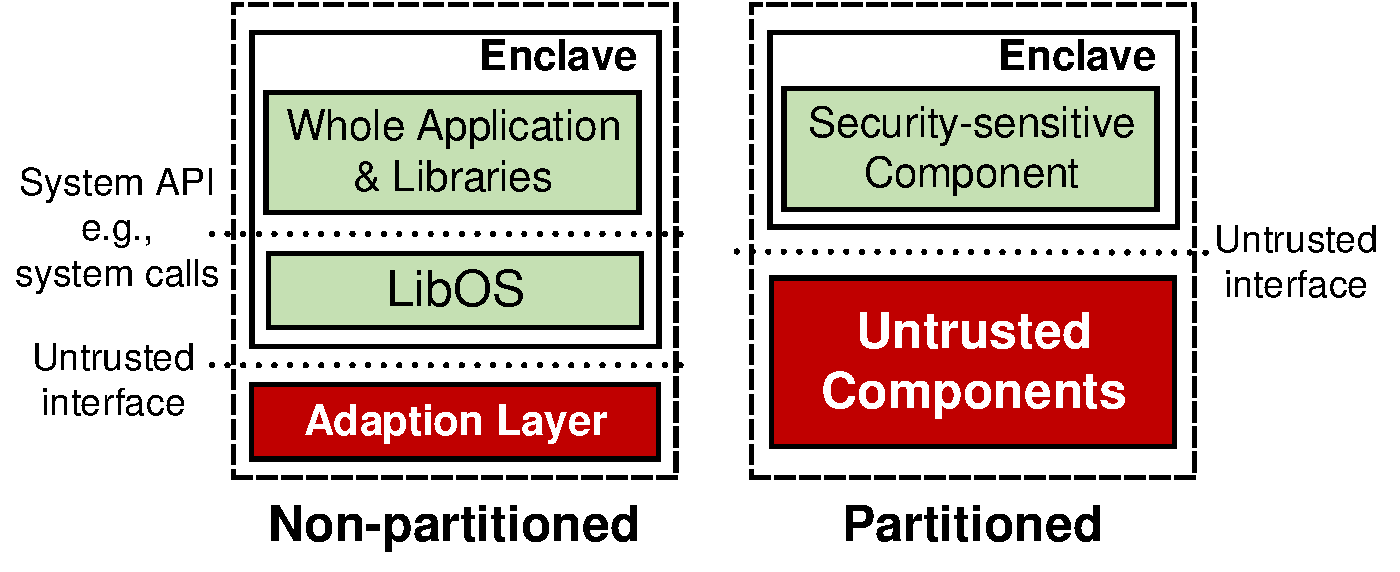
\includegraphics[width=1.0\linewidth]{libosvssdk.pdf}
\footnotesize
\caption{
Comparison between the Non-partitioned model (e.g., Haven)
and partitioned model for protecting applications in enclaves.
Green (light) boxes are trusted components and red (dark) boxes are untrusted.
The non-partitioned model yields a larger TCB in the enclave,
while the partitioned model requires developers to determine the untrusted interface at the enclave boundary.
}
\label{fig:libosvssdk}
\end{figure}

\papersubsection{\sgx{} Enclaves}

\intel{} \sgx{} ({\it Software Guard Extensions})
are a set of new x86/x86\_64 instructions
introduced in the \intel{} Skylake processor family.
Using \sgx{}, an 
application can designate part of its virtual memory as an {\em enclave}.
The CPU ensures that the contents of the enclave never leave the CPU package unencrypted.
The CPU also measures the integrity of a binary loaded into the enclave, and offers remote attestation,
similar to a TPM~\cite{TPM}.

%%% create a protected memory region, called an {\em enclave}, inside it's virtual memory,
%%% where it can load its security sensitive data with hardware-enforced isolation from the untrusted OS. 
%%% The processor with \sgx{}
%%% guarantees that any data loaded in enclave
%%% stays encrypted in the DRAM, by using a secret key deterministically derived from the application's cryptographic measurement and the CPU secret. 

\sgx{} is an appealing tool for protecting small amounts of highly-sensitive data or code, because it can defend 
against a malicious or compromised OS, hypervisor, or even hardware peripheral.
For instance, Hoekstra et al.~\cite{sgx-workshop1} show how \sgx{} can be used
to build a trusted path from a video chat application to a GPU and network card, which maintains confidentiality and integrity of the
video stream, even if the OS is compromised.
Similarly, because DRAM contents are encrypted, \sgx{} can resist attacks such as cold-boot attacks~\cite{halderman09coldboot} or 
malicious peripheral devices~\cite{hudson15thunderstrike}.

%\fixmedp{The flow from here to partitioned apps doesn't make sense.  Why are we getting into \sgx{} problems, then partitioned vs non-partitioned, then back to more problems?}
\sgx{} provides useful building blocks for secure applications, but does not
absolve the programmer of all responsibility for reasoning about end-to-end security.
Bugs in the application or supporting libraries can still disclose sensitive data from an enclave,
and porting code into \sgx{} can be subtle.
Inputs and outputs of an enclave must be checked carefully, and application-internal functions 
may not be hardened to the level of network-facing application interfaces.

Fundamentally, this argues for some combination of static analysis
and runtime monitoring of 
enclave code.  This is greatly simplified when the enclave code is written in higher-level languages
with properties 
%amenable to analysis.
%with type safety, memory safety, and other 
%that provide important 
%safety properties,
such as type safety or memory safety. %, thereby reducing the likelihood of these vulnerabilities.
Ideally, one would formally verify security properties of enclave code~\cite{moat}; this verification is significantly aided by using 
higher-level languages amenable to formal reasoning.
%Verification is significantly harder
%with C/C++ or assembly languages.


%The rest of this subsection outlines several pitfalls in partitioning an application for \sgx{}.



%\paragraph{Side Channels and Denial-of-Service.}
%In the current \sgx{} design, side channels are a significant concern, and are out of the scope of this paper.
%A controlled channel attack~\fixmedp{cite} can single step enclave execution by inducing page faults
%in the enclave.  \sysname{} does not specifically defend against side channel attacks,
%and we expect that any solution to this problem involves redesigning the %division of labor in virtual
%memory management for enclaves.

%Similarly, there is no guarantee that a compromised application will ever %enter
%an enclave.  Denial-of-service attacks are out of scope for this paper.

%% \paragraph{Writes outside of the enclave.}
%% However, the security of \sgx{} enclaves is founded on trusting the code running inside the enclave.
%% \sgx{} allows the trusted code to read and write data structures 
%% outside of the enclave.  Thus, it is easy for a developer to inadvertently write
%% code that discloses a secret, say by using a library that memoizes intermediate results to the untrusted heap.
%% A fundamental requirement is that developers must be able to reason about (or assert)
%% what code can and can't access data {\em outside} of the enclave.
%% \fixmedp{Can we say anything about whether such tools exist before Civet?}

%% %\fixmedp{Do I recall correctly that you can easily write to data outside of the enclave?  If so, this seems like something easy to get wrong, especially 
%% %if a library memoizes intermediate results.  The developer needs to be able to tell 
%% %Unless I am full of shit, can we paragraph-ize this fixme?

%% \paragraph{Vulnerabilities in the isolated applications.} 
%% One of the major threats to enclave security is the vulnerabilities in the isolated code,
%% such as memory corruption bugs,
%% control flow or information flows, semantic bugs, and so forth. 
%% %Moreover, although \sgx{} code integrity guarantees make enclaves resistant to code injection,
%% %an attacker may still manipulate control flow using code-reuse attacks~\cite{code-reuse-attacks}.
%% Moreover, recent research~\cite{hudata} shows that even with control flow integrity,
%% attackers can still manipulate the execution to leak the secrets through information flow.



%%% \sgx{} also proves the integrity of loaded binaries to remote trusted entities
%%% using mutual attestation based on a symmetric key generated from the measurements of communicating entities.
%%% \sgx{} usage model mostly involve the launched enclave mutually attesting the trusted host
%%% to obtain provisioning of security-sensitive information
%%% through a trusted channel. Such an execution model leverages resources such as CPU and DRAM from vulnerable untrusted \sgx{}-enabled hosts owned by cloud providers
%%% by extending the trust from
%%% the hosts owned and trusted by the clients or service providers.
%%% For instance, \sgx{} can isolate the decoder engine in an enclave
%%% after authenticating the customers to enforce Digital Right Management (DRM) even if the digital data is hosted on an untrusted cloud server.

%Use cases of \sgx{} mostly involve the launched enclave
%retrieving a cryptographically signed attestation from the processor,
%to exchange security critical information with remote servers through secured channels.
%The effect is equivalent to expanding the trusted space from remote servers
%to the local end, to harness local resources such as CPU and DRAM.

%One must note that \sgx{} only promises the integrity of application binaries
%initially loaded in enclaves.
%The gap between integrity of binaries and complete security has to be filled
%by ones who develop and approve the applications.
%More specifically, the clients are responsible of
%testing whether the applications contain any vulnerabilities
%that lead to information leak.
%To minimize the risk of leaving any flaws in the applications unintentionally,
%developers often tend to cut down the trusted computing base (TCB)
%of the applications. With smaller TCB, clients who launched the enclaves
%can more easily reason about the thoroughness of securing the execution.

%%% The key strength of \sgx{} enclaves over other software-based isolation framework such as
%%% {\em Flicker}, {\em Inktag} or {\em Virtual Ghost} is
%%% the ability to defend against attacks at the hardware level.
%%% These software-based solution often
%%% rely on a hypervisor below the OS to isolate the applications.
%%% If the hardware is attacked,
%%% the attackers may still bypass the software checkpoints,
%%% or directly steal confidential information from the DRAM.
%%% For \sgx{}, the only hardware included in the TCB is the CPU package,
%%% and in practice CPUs are believed to be hard to attack.
%%% Using techniques like cold-boot attacks~\cite{halderman09coldboot}
%%% to peek into DRAM content,
%%% or intruding the boot process using corrupted peripheral devices like Thuderstrike~\cite{hudson15thunderstrike}
%%% will affect any software-based isolation, but not \sgx{} enclaves.



%To achieve smaller TCB, the software development kit of \sgx{}
%intends to encourage developers to partition the applications and
%keep only security sensitive components in the enclaves.
%Such an intention is exactly contradicted by the trust model of \haven{},
%which must trust the loaded application as a whole.
%Except for the cases in which the whole applications must be secured,
%\haven{} actually downgrades the trustworthiness of enclaves.
%Figure~\ref{fig:libosvssdk} shows the comparison of the two models.

%%% In prior works using \sgx{} enclaves to secure applications,
%%% developers choose between two different programing models: the {\em library-OS-based} and the {\em partitioned} model (as shown in Figure~\ref{fig:libosvssdk}).
%%% In the libOS-based model, developers run the whole standalone,
%%% legacy application inside the enclave, using \sgx{} such as {\em Haven} or {\em \sgx{} libOS} to facilitate the rich OS features.
%%% The main benefit of using \sgx{} is that developers only have to employ minimal efforts to port any existing application.
%%% Even when designing new applications, developers bear no responsibility
%%% of identifying and reasoning about
%%% the security sensitive part of the application.

%%% However, when using libOS-based model, a sophisticated legacy application
%%% will yield huge trusted computing base (TCB) in the enclave,
%%% aggravating the risk of leaking information through vulnerabilities inside the enclave.
%%% Known bugs such as {\em the heart-bleeding bug} has shown that
%%% running security sensitive code like an encryption engine, and management code such as heart-beating service in the same address space
%%% can cause vulnerabilities that compromise the security by leaking the encryption key.
%%% As a result, using a partitioned model, developers can isolate only the most security sensitive components in an enclave,
%%% and leave the remaining code outside to minimize the TCB.

%%% Developers have to define the {\em untrusted interface} 
%%% to allow parts of a partitioned applications to interact.
%%% The untrusted interface is used either by the the untrusted components
%%% to trigger execution of the isolated components,
%%% or by isolated components to use untrusted rich OS features, such as networking for provisioning and sending the execution output to the remote hosts.
%%% Unlike the libOS approach that has a fixed untrusted interface (for different applications) at their interaction boundary with the OS,
%%% the width of untrusted interface for a partitioned application is up to developers' design.
%%% The \intel{} SDK for \sgx{} supports a set of syntaxes to specify the type and direction of flow for parameters of the untrusted interface, and enforces primitive
%%% type-checking of incoming values on transition to enclave.

%%% The trade-off between the libOS-based and partition model is based 
%%% on ease of development, the width of untrusted interface,
%%% and size of TCB.
%%% The benefit of the libOS-based model is that developers can save the effort
%%% of determining what to execute in the enclave,
%%% and whether the execution is safe,
%%% because the whole application is wrapped in the enclave.
%%% However, the risk of having vulnerabilities in the applications
%%% is not reduced, but in fact amplified due to the addition of
%%% the \sgx{} (e.g., the Haven binary yields around a few hundred MBs) to TCB.
%%% On the other hand, if the developers are willing to spend effort on carefully identifying the untrusted interface and re-designing their application around this interface, the partitioned model can improve security guarantees by minimizing the attack vectors.

%%% The goal of \sysname{} is to provide the benefits of both models.
%%% \sysname{} support a partitioned model
%%% for developers to isolate security-sensitive part of a \java{} application in enclave,
%%% and provide a language-based tool to automatically partition
%%% the minimal supporting classes to generate the enclave image.
%%% Even in the case where the isolated component need to frequently interact with the untrusted component or the OS,
%%% the language protection technique of information flow tracking
%%% guarantees that the secrets in the enclave are never leaked
%%% without the developers explicit consent. 


\papersubsection{Two \sgx{} Usage Models}
\paragraph{Non-partitioned applications}
One model for using \sgx{} is to run an entire application in the enclave.
This is exemplified by Haven~\cite{baumann14haven}, which runs a \win{} application and all supporting libraries
on top of a library OS (\libos{}) inside an enclave.  This approach is illustrated on the left side of Figure~\ref{fig:libosvssdk}.
The non-partitioned model offers simple deployment, requires no application changes, and can provide practical benefits, 
such as protecting an application from an untrusted cloud hypervisor.
In the case of Haven, running an unmodified application bloats the TCB by 5.5 billion lines of code.
%By pulling millions of lines of extraneous code into an enclave, there is a significantly increased risk 
%of vulnerabilities that disclose
%sensitive data, such as Heartbleed~\cite{heartbleed}.
%\fixmebj{Move heartbleed example to next subsection for motivation.}


\paragraph{Partitioned applications}
One can reduce the in-enclave trusted computing base by paring it down to only the
security-sensitive pieces of application logic (right side of Figure~\ref{fig:libosvssdk}).
%This paper focuses on a second usage model for \sgx{} enclaves, where an application is partitioned into
%the untrusted and trusted sides 
%Only sensitive data and computation are placed inside the enclaves.
This partitioned model requires the developers to
identify what in the application should be protected; harden an interface between trusted and untrusted components; 
%modify the application source;
and reason about potential information flows at the enclave boundary~\cite{kilpatrick2003privman}.
This effort can be non-trivial and subtle, but for application developers motivated by interests such as 
regulatory compliance or competitive advantage in business, the additional effort can yield a much smaller trusted computing
base (TCB), and thus a reduced attack surface.
A key goal of \sysname{} is to minimize the developer's effort to partition an application---both in lines of 
code changed, and in leveraging language analysis to reason about narrow points in the application's data and control flow at
which to establish an interface between trusted and untrusted components.


%\fixmebj{Talk about protecting untrusted app from os or hypervisor is orthogonal.}



\papersubsection{Challenges in Partitioning \java{} Applications on \sgx{}}

Using a higher-level language can be useful to reduce the risk of semantic errors in an application,
yet there are several fundamental, technical challenges to using a managed language, like Java,
in an \sgx{} enclave.
In part, this is simply an artifact of the \sgx{} design, which is designed
for native libraries.
%To our knowledge, no previous work has successfully executed a \jvm{} inside an enclave.

%% For developers who prefer implementing applications in a higher-level language like \java{} ---
%% to limit the vulnerabilities in the applicatins,
%% and use the partitioned model to protect the applications with \sgx{}
%% --- to reduce the TCB of enclaves,
%% the combination of two protections can be challenging.
%% For starter, \sgx{} enclaves are not designed to run any applications that are not native binaries.
%% Even though using the non-partitioned model with a \sgx{} like Haven
%% can potentially run \java{} applications with the whole \jvm{}
%% inside the enclaves,
%% the technical effort required is non-trivial,
%% and no previous work has demonstrated any successful case yet.
  
%% \paragraph{Introducing \sgx{} to \java{}.}
%% We identity several challenges in presenting the \sgx{} protection to
%% \java{} applications, to allow them to isolate their security-sensitive components.
%% The challenges are in fact more than just the technical efforts
%% to design a wrapper API for \sgx{} instructions.
%% The fundamental gap between the requirement of using \sgx{} enclaves
%% and the characteristics of the \java{} language
%% is the primary pitfalls in combining them.
%% The requirements are not limited to \java{} and \sgx{},
%% but can apply to other languages and hardware protections.
%% \fixmets{The discussion of the three primary problems must match section~\ref{sec:concept}.} 


%%% \sgx{} enclaves provide strong isolation guarantee for applications,
%%% against the malicious or vulnerable application components, system stack,
%%% and hardware (except the CPU itself).
%%% However, the security guarantees of the \sgx{} enclave is dependent on whether the developers design perfect applications without exploitable vulnerabilities that may compromise the application's security.
%%% As the application developers are not perfect,
%%% even applications or components isolated in enclave can face threats to their security.
%%% As follows, we discuss a few potential threats
%%% to the enclave security,
%%% even under the assumption that the \sgx{} hardware is implemented as completely secure --- which can be another threat otherwise. 

%\fixmedp{I roughly want the rest of this section to have a problem, explanation, solution structure, with the overall theme being that this is subtle and we really need some analysis tools to get this right}


%% \paragraph{Applications are not perfect} 
%% The \sgx{} hardware cannot prevent applications from copying secrets out of the enclave without limiting functionality.
%% The trusted isolated components can copy any sensitive data from the enclave to the unencrypted memory, and potentially leak the enclave secrets.
%% The primary risk in the isolated components
%% is often memory corruption vulnerabilities, such as buffer overflow,
%% %Because in enclave applications can access any part of out-of-enclave memory unrestrictedly,
%% prevalent in applications that are not implemented in type-safe languages.

%% The best known technique to prevent vulnerabilities is to model the applications and verify them using {\em formal verification}.
%% While Sinha et.al.,~\cite{moat} use formal verification to prove confidentiality of enclave programs, it is impractical to accurately model complex sophisticated applications.
%% As a result, in addition to formal verification, maintaining smallest TCB
%% in the isolated components is the most practical approach 
%% to ensure enclave security,
%% and is the main reason to choose partitioned programming model over
%% libOS-based model.


%\begin{figure}[t!]
%\centering
%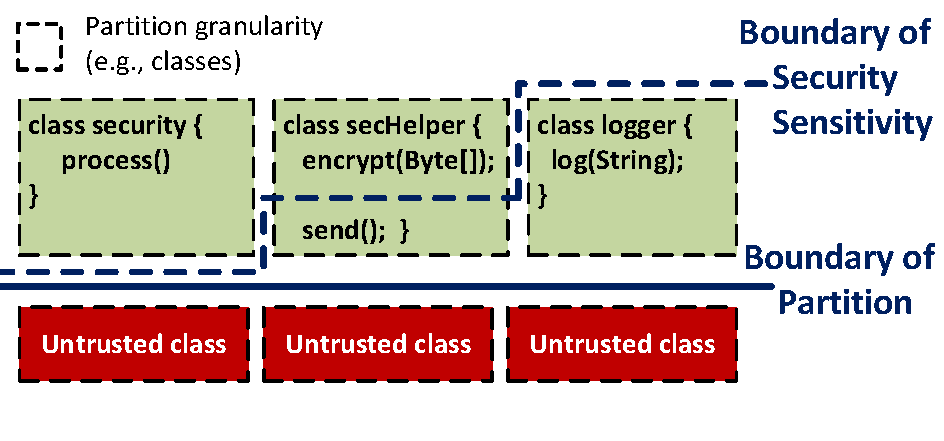
\includegraphics[width=\linewidth]{figures/partition.pdf}
%\footnotesize
%\vspace{-0.3in}
%\caption{
%Partitioning --- either manually or by automated tool ---
%often causes wider boundary of partition than the actual security sensitivity boundary
%due to (a) design granularity : {\tt SecHelper} contains a {\tt send()} method that is not partitioned from the rest of the class by design.
%or (b) better performance :  the less security sensitive {\tt logger} class is kept in 
%the privileged level to service frequent method calls. \fixmebj{Initial letter of all 
%class names must be Capital.}
%}
%\label{fig:partition}
%\end{figure}

%However, even if developers partition the applications and run only
%security sensitive components in the enclave,
%the developers may still leave some code irrelevant to
%enclave secrets inside the enclave.
%The reasons of having more-than-minimal TCB in enclaves
%are often that developers have to partition code in the granularity of source files or functions,
%or developers have to import more code to limit the width of interface and
%the frequency of interaction with the untrusted code.

\paragraph{\bf Challenge I---Cleanly partitioning classes and objects (\S\ref{sec:concept:partition})}
Java encapsulates the placement of object data and code within virtual memory, which facilitates features
like inheritance and garbage collection, but complicates integration with \sgx{}.
To program for an \sgx{} enclave, the developer must understand which regions of virtual memory 
are in the enclave, and which are outside of the enclave.
Note that \sgx{} allows code in the enclave to access memory
outside of the enclave.  Thus, it is easy for a developer to inadvertently write
code that discloses a secret, say by using a library that memoizes intermediate results to the untrusted heap.
Further, when a Java class inside of an enclave inherits methods or fields
from a parent class that is placed outside of the enclave, it is easy to 
inadvertently pass sensitive inputs to a function outside of the enclave,
or update a class field outside of the enclave.

In order for programmers to be able to sensibly program for \sgx{}, they need
a model of how objects are placed inside and outside of the enclave at runtime, as well as a model
for if and when updates to objects are propagated across the enclave boundary.
%\fixmedp{please fact check this rewrite, and make sure I am on the right track}
%\fixmebj{Looks ok to me. I will let Chia-che remove the fixmes.}
%% \sgx{} enclaves isolate the trusted components from the rest of the application,
%% and makes sure that no code or data
%% is shared between the trusted and untrusted parts.
%% For languages like C, which statically define functions and variables, it is easier for developers to cleanly
%% draw the line between trusted and untrusted components.
%% However, for a managed language like \java{}, a class can be inherited by other classes,
%% or referenced as other classes's fields, so the class may belong to both
%% untrusted and trusted components.
%% As a result, developers may struggle to manually partition the \java{} classes, especially if large portions of the classes are imported from libraries and not written by themselves.

%Reasoning about where in a program to draw the line between 
%trusted and untrusted code is subtle.
%On one hand, the developer has an incentive to minimize the size of the 
%API between the enclave and untrusted code, as well as an incentive to
%minimize the total code in the enclave.  These goals can sometimes be at odds.
%Each entry and exit to an enclave has a cost roughly comparable to a
%process context switch\fixmedp{right?}; an easy way to reduce enclave entries and exits is to simply 
%pull more code into the enclave, which increases the size of the TCB. For instance, in Figure~\ref{fig:partition}, even if the class {\tt Logger} is not security sensitive, 
%it is included in the enclave side of boundary of partition to avoid frequent entries and exits out of enclave.


%\fixmedp{I'm not sure how to explain Figure~\ref{fig:partition}, but it needs an explanation.}

%Fundamentally, the art of paritioning an application is to find a ``pinch point'' or
%``narrow waist'' in the application, where there is a natural point to insert an API and 
%security checks.  This is indeed as much art as science, often done manually by experts\fixmedp{any more supporting evidence or cites?}. Moreover, different classes of applications in managed languages like \java{} are tightly coupled; and it is necessary  to widen the boundary of partition to include some non-sensitive code in the trusted component.
%For instance, in Figure~\ref{fig:partition}, even if the {\tt send()} method is not security sensitive, it has to be included in the enclave code because of the design of the class {\tt SecHelper} to achieve a clean partition of the application.
%It is unlikely that the average developer will successfully navigate this design process without analysis tools, such as \fixmedp{examples?},
%to help identify these natural division points.


%% Experts can use a manual partitioning technique to achieve smallest TCB for the isolated components compared to automated tools.
%% However, the manual partitioning costs a lot of effort,
%% and rare expertise, lack of which can cause larger TCB.

%% Neither manual nor automated partitioning is perfect:
%% the resulted boundary of partitioning often has a gap from the actual boundary of security sensitivity (as shown in figure~\ref{fig:partition}),
%% leaving more code in the privileged level
%% than what's actually needed.
%% Having the gap between the ideal and resulted boundary
%% is mostly inevitable, due to multiple reasons.
%% One common reason is the granularity of partitioning,
%% which can vary from a binary file, a component, a source file,
%% a class, a method (a function) to a line of code.
%% Another reason is that a component or a method may be too frequently called
%% by the security sensitive code,
%% laying the boundary between the component or method from the security sensitive side may bring too much overhead or risk,
%% because the execution crosses the boundary too often.
%% Therefore, developers often will balance among the effort of partitioning,
%% risk or cost of communicating between different partitions,
%% and minimizing the TCB in the security sensitive parts.

%\fixmedp{Maybe move the commented paragraph below down into the design section?  I'd like to downplay the plugs for our work here, and instead fulfill these promises later}
%% \sysname{} automates partitioning of applications,
%% based on the boundary at the classes which the developers marked
%% as the interfaces of the enclave.
%% Only the classes that are depended by the marked classes
%% will be included in the enclaves,
%% to minimize the TCB.
%% Although not all classes pulled into the enclaves
%% are necessarily security sensitive,
%% the enclaves are protected from the potential vulnerabilities in those classes,
%% by the security guarantees of \java{} language,
%% and the information flow tracking in \sysname{}.

%Another threat to \sgx{} is the vulnerability of the 
%security sensitive code running in the Enclave. The 
%main guarantee of \sgx{} to isolate the secure data 
%from other components and privileged OS is undermined 
%if the Enclave code can be tricked to leak the 
%security sensitive data to the attacker. Executing 
%buggy code in \sgx{} enclave can inadvertently leak 
%information if the attacker can exploit memory-safety 
%vulnerabilities like buffer overflow and dangling 
%pointers.  

% Cumbersome and approximation to partition code
%The developers have to manually partition their code 
%into security sensitive and insensitive part. If this 
%partitioning is done by a novice developer, some of 
%the security insensitive parts of the application can 
%end up in the security sensitive part, increasing the 
%Trusted Computing Base(TCB). Moreover, the 
%partitioning of code is not straightforward, which 
%can also contribute to a less stricter TCB. The bigger the TCB, the more %vulnerable is the Enclave code to attacks.

% Buggy Code leads to inadvertant information leakage


% \sgx{} code only Integrity protected not confidential
%Moreover, \sgx{} only protects the integrity of the enclave code. The security critical part of the application is stored in plaintext while the secret data is provisioned securely after attestation. However, \sgx{} does not protect the confidentiality of enclave application code which may be executing a secret algorithm. \fixmebj{Talk more about the problem motivating security tag preservation.}
%\sgx{} can natively guarantee either code integrity or
%code confidentiality (as part of the enclave data), but not both.
%If application code is included in the enclave measurement and
%verified by the hardware,
%the code must stay in plaintext as part of the enclave image.
%If any code is stored or provisioned in encrypted forms,
%the application or infrastructure in enclave must dynamically load
%the code after decryption.
%Supporting dynamic loading makes enclaves open to code injection
%if the applications have exploitable vulnerabilities.

\paragraph{\bf Challenge II---Dynamically loading byte-code with integrity (\S\ref{sec:concept:loading})}
\sgx{} establishes trust by verifying the integrity of the code in the enclave.
Therefore, enclaves must be bootstrapped with static, native binaries.
%that have consistent measurements.
However, \java{} classes are shipped as byte-code,
and dynamically loaded by \jvm{}s.
The subtle security challenge for a Java developer 
is ensuring that, when a class is dynamically loaded into an enclave, by passing a string name of the class,
the application needs to be able to verify that this is a trusted class file
and that the initial state of the class is correct.
Thus, we introduce techniques to manage trust and verify the integrity of 
dynamically loaded code, including encrypted class files.

We note that using byte code is both a liability and opportunity.
One could pre-compile byte code to native code on a trusted host, and simply run the signed native code.
However, this foregoes the opportunity for performance-critical enhancements
such as profile-guided optimization or heap management optimizations for
smaller heaps.  Version 1 of \sgx{} only has up to 128 MB of total enclave page cache;
Version 2 will relax this extension.  As long as \sgx{} is a moving target,
we expect there will be value in the ability to dynamically optimize the
in-enclave code for the constraints and application behavior at runtime.

%This means the \sgx{} enclaves can only guarantee the code integrity of the initially loaded infrastructure, which in turn has to
%verify the integrity of classes dynamically loaded.
%\fixmedp{Can you say a bit more about why this is hard or interesting?}

%The hardware-level \sgx{} code integrity mechanism is based on a cryptographic
%signature of a static binary in plaintext.
%If any application dynamically loads any code after the enclave's initial measurement,
%the initial application must be trusted to attest the loaded code.
%The subtle tension is that there is no way to protect the confidentiality of
%a secret algorithm, except by dynamically loading an encrypted binary.
%Dynamically loading code increases the risk of code injection attacks and other control flow compromises. The interpreted and managed languages effectively compound the
%risks by dynamically loading all the application code.

%Any application partitioning solution that protects sensitive algorithms and data
%must have a robust dynamic loader that can measure encrypted libraries or classes.
%\sysname{} includes a loader that can measure encrypted class files,
%provisioned from a trusted host.

%% \sgx{} enclaves require code integrity in the isolated applications.
%% If the code integrity is not maintained, adversaries can corrupt the enclave code to
%% force the applications to leak the information provisioned from the remote,
%% trusted hosts.
%% \sgx{} hardware only guarantees
%% the integrity of the code initially loaded into the enclaves.
%% However, if an application choose to dynamically
%% load any code after the enclave starts,
%% the application is responsible for the integrity of the code loaded.
%% The fact that dynamic loading of applications, libraries or components
%% is a feature that can potentially make enclaves vulnerable and open to code injection,
%% raises concerns against supporting managed languages in the enclaves.

%% On the other hand, code confidentiality can be a desirable feature,
%% for application developers who prefer keeping the secret sauce of their algorithms concealed.
%% To enable the feature of code confidentiality in enclaves, the protected code must be dynamically loaded into the enclave,
%% because the \sgx{} hardware only accept
%% the initial loaded code to be in plaintext.
%% \sysname{} provides both code integrity and confidentiality by verifying
%% every classes dynamically loaded into the enclaves,
%% and allows loading classes provisioned from trusted hosts.


%% In general \sgx{} enclaves are prone to having side channels, such as timing channels. Because \sgx{} relies on the untrusted OS for paging,
%% an enclave will always leak page fault addresses, except the lower 12 bits (offsets in pages).
%% Such a leakage gives the untrusted OS to amplify the side channels,
%% by forcing page faults on every instruction or memory access.
%% This so-called {\em Controlled Channel Attack} is common to all applications who use \sgx{} protection, regardless of the programming models.
%% \sysname{} does not specifically defend against side channel attacks.

%% \paragraph{Denial-Of-Service Attacks}
%% \sgx{} is not designed to be safe against denial-of-service attacks.
%% Because the untrusted OS still controls the host resources,
%% there are countless ways to prevent an enclave from making progress.
%% For example, the OS can simply starve the enclaves by
%% never scheduling CPU, memory or other resources to the enclaves.
%% \sysname{} does not specifically defend against denial-of-service attacks.

\paragraph{\bf Challenge III---Seamless access of in-enclave objects (\S\ref{sec:concept:accessing})}
Java code outside of the enclave must be able to call enclave entry points and 
have some notion of objects that are inside the enclave.
Unlike C, where most function addresses are determined once
at the dynamic linking phase,  Java identifies most functions through
object references (e.g., {\tt Foo.toString()}).
Thus, the untrusted code must be able to reference
objects inside of the enclave in a way that makes sense when
the untrusted code behaves correctly, but that does not create unexpected information flows 
out of the enclave.
Similarly, the developer needs a constructor interface to declare which dynamically-created
objects should be placed in the enclave and which should be outside of the enclave. 


%% For native binaries, enclave entry points are statically inserted
%% into the untrusted code
%% at explicit locations known to interact with the enclaves.
%% However, for \java{} applications, instantiating or calling methods
%% on isolated components must dynamically trigger enclave entry.
%% For instance, calling the {\tt toString()} method of any object 
%% may trigger enclave entry based on whether the object's reference type is in the enclave.
%% Moreover, the the objects and methods determine the entry targets (the locations where the execution transfer after entering the enclaves) and the arguments passed into the enclaves at entry.
%% Unlike native binaries, the code behavior at enclave entry must be determined at runtime.
%% \fixmedp{I don't understand this point yet.  Is the issue that the untrusted code needs to track
%% opaque references into the enclave?  Can you explain more?}


%The \sgx{} hardware ensures that the enclave only has fixed number of entry points 
%(exactly one location where the execution starts, but multiple pre-defined locations 
%that the execution can jump to). However, for an application written in a language like JAVA with a virtual machine or interpreter, there are no clear entry points separating 
%the trusted and untrusted components. Moreover, due to the approach of executing intermediate code, it is also difficult to determine the entry points at runtime.

%Just separating an application into parts based on security sensitiveness is not enough to securely isolate the two parts using \sgx{}. In addition to application partition, there is a need to automatically determine the entry points without offloading the effort to the developers. \sysname{}  automatically identifies and exports all untrusted interfaces to the isolated classes at build time.

%\paragraph{Discussion.}
%This section has outlined several pitfalls for developers of partitioned applications.
%These common pitfalls render the hardware protections of \sgx{} useless.
%Language-level analysis can automate error-prone reasoning in the best case, or, in the worst case, 
%can at least offer invaluable guidance to the developer.  For \sgx{}-style
%hardware to be useful to a wide array of developers, developers need language-level
%tools that can also factor in hardware-level protection mechanisms.

\begin{comment}

\papersubsection{The Challenges of Combining Language and Hardware Protections}

Language and hardware protections provide varying benefits
to application security:
Languages improve the internal security inside the applications,
while hardware provides the base defenses that cannot be easily overridden or bypassed.
Commonly security experts exploits both types of protections
to further harden the security of applications.
For example, hardware protections may take information from the language runtimes or compilers to enforce the security policies,
or language protections may rely on hardware protections to bootstrap the initial trust they need. 

However, the combination of language and hardware protections is more
like a trick of the trade for security experts:
the use of hardware protections is deeply buried in the design of language protections,
so that users (application developers) lose direct access
to the security guarantees and features provided by the hardware.
\fixmets{Think of an example: Maybe TPM.}
The approaches of combining language and hardware protections are mostly ad-hoc to the use cases,
i.e., how one protection is used to improve or reinforce another.

There are two reasons for why combining language and hardware protections
is so inevitably hard.
First, hardware protections often have restrictions
on the languages that must be used
to access the security guarantees and features of the hardware.
For example, \sgx{} requires the loaded code to be implemented in C or C++,
or any languages that can compile applications into static binaries.
The restriction is not simply a design decision
made by the hardware or its SDK,
but a result of the fact that \sgx{} requires a static image to guarantee the integrity of execution.
On the other hand, if the language used is a managed language like \java{},
accessing \sgx{} hardware will be cumbersome,
because it is hard to provide any APIs to allow direct access to the \sgx{} hardware,
to harvest its security guarantees
or to utilize its features.

\begin{figure}[t!]
\centering
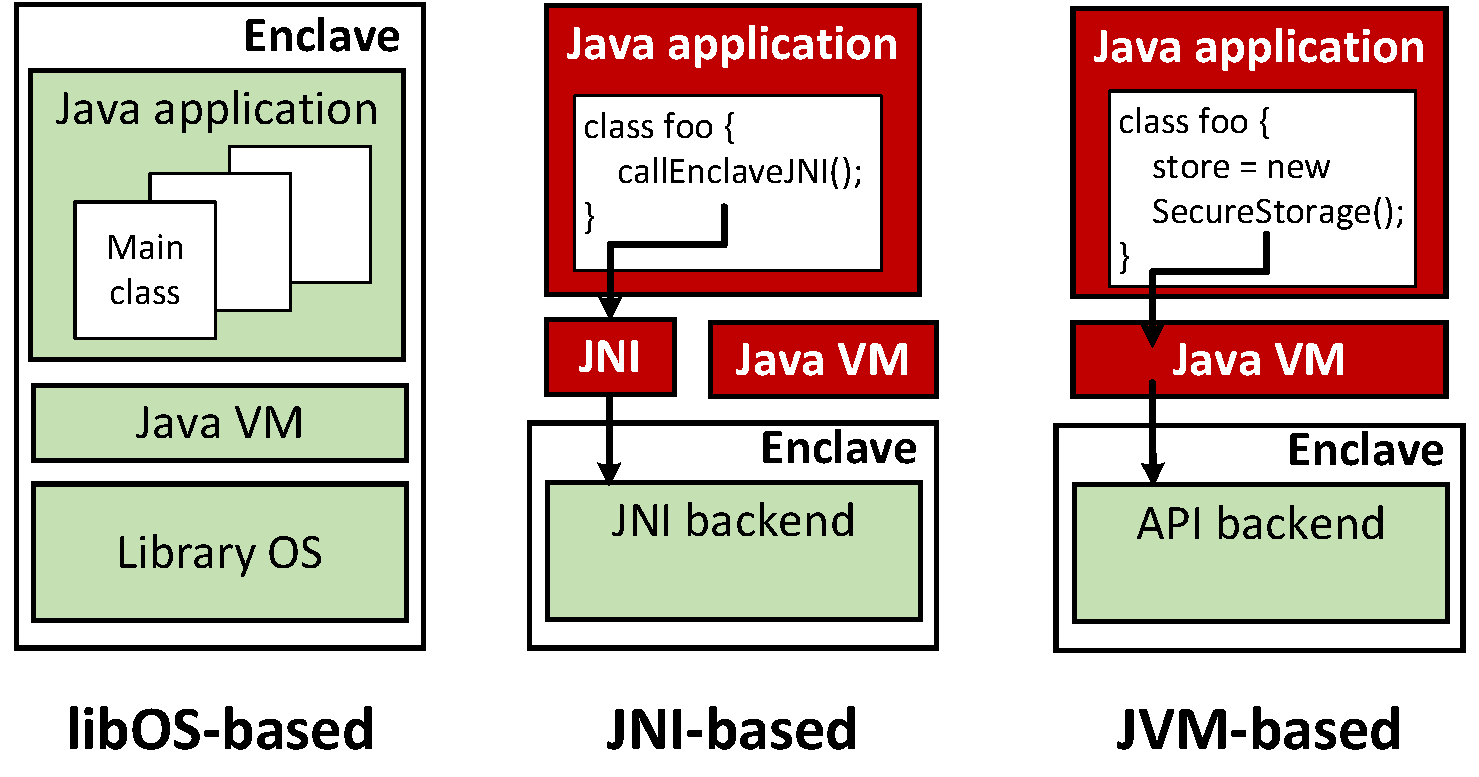
\includegraphics[width=\linewidth]{figures/alternatives.pdf}
\footnotesize
\caption{Alternative approaches to access \sgx{} hardware protection from \java{} applications.
The {\em \libos{}-based} approach runs the whole \java{} applications in the enclaves. 
The {\em JNI-based} approach uses JNI to run the security sensitive operations inside the enclaves.
The {\em \jvm{}-based} approach requires the \jvm{} to provide APIs to support common use cases of the enclaves.
Green (light) boxes are trusted components and red (dark) boxes are untrusted.
}
\label{fig:alternatives}
\end{figure}


Figure~\ref{fig:alternatives} illustrates the alternative approaches
to access \sgx{} hardware from \java{} applications:
The first approach is to run the whole \java{} applications with the \jvm{} inside the enclaves,
using a \libos{} ({\em \libos{}-based}).
This approach can secure applications as a whole,
but won't support any partitioned model for programming.
Another approach is to implement a JNI that create and interface with the enclaves
to run the security-sensitive operations ({\em JNI-based}).
The JNI-based approach is flexible enough for application developers
to implement the isolated components as well as the untrusted interface,
but requires developers to have the knowledge of
enclave implementation.
More importantly, the isolated components can only be developed in C or C++
language, so the applications lose the language protection of \java{} inside the enclaves.
A more plausible approach is to provide enclave-backed APIs
from the \jvm{},
to support common use cases ({\em \jvm{}-based})), such as a secure key-value store~\cite{vc3}.
Although the \jvm{}-based approach can save the application developers' effort
of implementing isolated components,
the use cases is limited to the pre-defined operations provided by the \jvm{} or the companion frameworks.
Because the backend implementation (isolated components and untrusted interfaces) in the \jvm{}-based approach is the same as the JNI-based approach,
the same language restriction also applies here. 

\end{comment}

%- Motivate the problem.
%- List all attack vectors
%- How can JAVA help?

\paragraph{Discussion}
Partitioning an application requires some input from the developer in order to identify 
sensitive data and code.  Each of the challenges above highlight cases where
Java either hides important information from the developer, or otherwise useful runtime
techniques can thwart the isolation benefits of using a hardware mechanism like \sgx{}.
A higher-level goal of \sysname{} is to provide constructs for the developer to specify
her goals, such as which objects should be isolated in an enclave,
and to have the language runtime use these developer-provided hints to 
make judicious choices on issues such as data placement.
A related goal is not eroding the benefits of developing in a high-level, managed language runtime.


%% The combination of language and hardware protections
%% is a technique used by many previous works.
%% However, the approach often seems like a trick of the trade for security experts:
%% the use of hardware protections is often deeply buried in the design of language protections,
%% as the underlying mechanism to bootstrap the trust
%% or to secure the core components of language protections.
%% %so that users (application developers) lose direct access
%% %to the security guarantees and features provided by the hardware.
%% %\fixmets{Think of an example: Maybe TPM.}
%% %The approaches of combining language and hardware protections are mostly ad-hoc to the use cases,
%% %i.e., how one protection is used to improve or reinforce another.
%% This work chooses a different approach,
%% by allowing \java{} applications
%% to straightforwardly utilize the protection of \sgx{} enclaves,
%% while still benefit from the safety properties
%% and advanced language protections from \java{}.
%% As a result, our framework also opens the win-win opportunity for
%% hardening both \sgx{} and \java{} protections.
%% \fixmedp{I also don't understand the point of this discussion.  What do you want the reader to learn from this?}

%\papersection{Threat Model}
\label{sec:threat}

In this section, we discuss the threat model of \sysname{},
including the adversaries,
and the components that must be trusted.

\paragraph{Adversaries}
We assume the same adversaries as other \sgx{} enclaves.
Any part of the system stacks, including the OSes,
device drivers, hypervisors, and even hardware,
such DRAM, GPU, buses, and peripheral devices, can be malicious
and attempt to attack the enclaves.
%The only trusted component is the CPU package, including L2 and L3 caches.
The attackers can perform any form of
online and offline attacks.
We also assume the attackers own all information
about \sgx{} hardware implementation, as well as every part of our solution.

We focus on the adversaries that target on
exploiting vulnerabilities in the isolated applications.
The attackers can manipulate any input to the application interfaces,
or the untrusted interfaces of the enclaves.
%Attackers may apply any techniques that compromise a regular privileged applications to compromise enclaves.
The vulnerabilities that attackers can exploit may not only fall in applications, but also in the infrastructures,
such as the libOS, the \java{} VM, JNIs and low-level interface to architecture.

%The only adversaries that are not addressed in \sysname{} are
%attackers exploiting {\em side channels} and
%{\em denial-of-service attacks}.
%Side channels, or even controlled channels, is a known problem of \sgx{} enclave
%and we expect to solve the problem in the future with
%stronger architectural support.
%Denial-of-service attacks are often considered benign for enclaves,
%because it only affect the ability of an untrusted host to legally access
%critical resources.

\paragraph{Trusted Components}
We trust any components loaded inside an enclave,
including the infrastructure (details discussed in Section~\ref{sec:implementation}), %(low-level interface, the libOS, \jvmname{}),
all supporting classes and their JNI,
and other resources or classes provisioned from remote hosts.
%All trusted components must be verified by either \sgx{} hardware or the infrastructure against their cryptographical measurements or checksums.
The implementation of \sgx{} hardware is also trusted to be invulnerable,
and use adversary-resistant key generators that cannot be compromised
by online or offline techniques.
We also assume \intel{} CPUs are resistant to direct, physical attack to the CPU packages, either to modify or peek into the chips.

\fixmets{Now JIT'ed code is not giving me error, but in case it fails later, we have to flip this discussion.}
We support running \java{} application both with and without JIT optimization.
Running \java{} application with JIT optimization
improve the performance of execution,
but can cause massive increase of the TCB of enclaves.
In case that JIT optimization is enabled in the enclaves,
the JIT compilers (\java{} VMs often have multiple JIT compilers, e.g., \jvmname{} has two) must be trusted by the users,
to always generate correct and invulnerable binary code.


%Note that in \sysname{} we disable JIT compiler that used to improve \java{} execution performance.
%The choice of disabling runtime compilation is due to the concerns that
%JIT compiler may largely extend the TCB because it must be trusted,
%and any bugs in different versions of compilers
%may causes code behaviors than what developers have tested and expect.
%Another practical reason is concerning the complexity and
%resources required for running a \java{} compiler with library OS in an %enclave.
%However, we consider these limitations to be not fundamental to the approach, and we keep compiler support in \sysname{} as a future work.



%In term of architecture, we trust the implementation of \sgx{} hardware,
%to maintain invulnerable implementation of \sgx{} instructions,
%and using adversary-resistant key generators that cannot be compromised
%by attacker using online or offline techniques.
%The CPU must keep enclave contents encrypted in DRAM and low-level caches that are shared by multiple cores.
%We also assume \intel{} CPUs are resistant to direct, physical attack to the CPU packages, either to modify or peek into the packages.

%\sysname{} protects confidentiality and integrity of provisioned security critical data in the trusted part of an application written in a high level managed language like JAVA.
% from the privileged operating system and the untrusted part of the same application. 
%\sysname{} assumes that the \sgx{} instructions are implemented correctly in the processor, and the SDK do not contain exploitable bugs to leak information. In addition, \sysname{} trusts the Graphene LibOS and the JVM running in the enclave with the trusted part of the application to not leak information. Thus, the security of the provisioned data is limited by the correctness of the processor, \sgx{}, Graphene LibOS, and JVM. \sysname{} also trusts the trusted part of the application to not leak information explicitly. \sysname{} prevents the trusted part of an application from implicitly leaking information.

%Threats that we do not cover
%\sysname{} inherits the threat model of \sgx{}~\cite{sgx}.
%The adversary controls the cloud provider's complete stack, OS, hypervisor, BIOS, system management mode, platform firmware, and device firmware. The adversary can also probe the memory and manipulate the I/O, but cannot read secret present in the processor.
%\sysname{} do not defend against attack vectors such as side-channel, covert-channel and control-channel~\cite{control-channel}. Denial of Service (DOS) attack is not part of \sysname's threat model. Even if the OS never schedules the enclave program or the untrusted part of the application is manipulated to never enter the enclave, no provisioned secret is leaked outside the enclave.


\chapter{System Overview}
\label{chap:overview}

\makeatletter
\def\input@path{{overview/}}
\makeatother
\graphicspath{{overview/figures/}}

%\section{Introduction}
%\label{sec:dcache:introduction}

Operating System kernels commonly cache file system data and metadata in 
a virtual file system (VFS) layer, which abstracts low-level file systems into a common API, 
such as POSIX.  
This caching layer has become a ubiquitous optimization
to hide access latency for 
persistent storage technologies, such as a local disk.
%whether a local disk or a network appliance, 
%have substantially higher access latencies than RAM,
%this caching layer 
%% SOSP Space - kind of quacking on
%% Caching
%% the file system directory hierarchy is particularly important because 
%% low-level file systems often spread this information across 
%% multiple disk sectors.
%% If an application wanted to open a single file on a system without a directory cache, 
%% most low-level file systems would issue numerous disk reads to locate the file and check the permissions
%% on the file and its parent directories;
%% a directory cache can commonly avoid these reads.
The directory cache is not exclusively a performance optimization; it also simplifies 
the implementation of {\tt mount}-ing multiple file systems, 
consistent file handle behavior,
and advanced security 
models, such as SELinux~\citep{selinux}.



%\fixmedp{Be charitable to developers, make our strong claims positively (we are really smarties) rather than calling them dummies}


%% Many observation shows that, in most systems, operations to storage are often
%% dominated by hierarchical structure traversal,
%% and fetching metadata of objects.\fixmetsai{references here}~\citep{duchamp94nfs}
%% In many file systems, traversal and metadata fetching
%% create random access patterns,
%% which are slower than sequential access patterns
%% on many storage media, e.g. magnetic disks.

% dp: I think this is getting down in the weeds.  We need to make the case for the work 
%     more strongly and generally first
%% Directory entry cache, a.k.a \dcache{},
%% is an important optimization in Linux kernels
%% to reduce storage operations for traversal and metadata fetching.
%% The design of \dcache{} is comparable to \vnode{} in BSD and \dnlc{} in Solaris.
%% \dcache{}, as well as \vnode{} and \dnlc{},
%% can be explained as a file system layer that
%% responds to requests on a cache hit,
%% but passes requests down to lower-leveled file systems on a cache miss~\citep{zadok06, skinner93}.

%\fixmedp{F1: Maybe thread together an argument about why no one would have tried a one-hop lookup before?}


%\marginpar{\scriptsize \textcolor{blue}{ Michael, I think the high-order bits are mostly right on Fig~\ref{fig:dcache:lookup-frac},
%but these number may change a bit as we refine the measurement}}

\begin{figure}[t]
\scriptsize
\centering
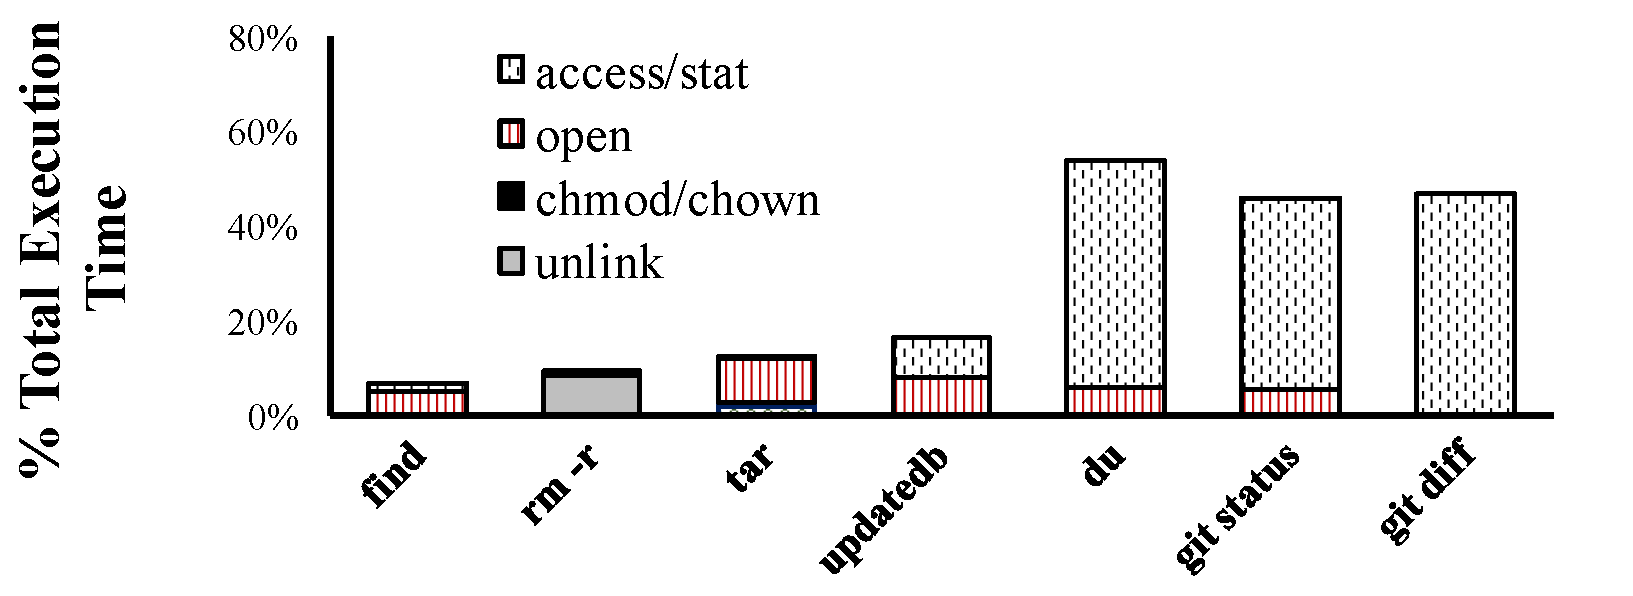
\includegraphics[width=5in]{dcache/plots/syscall-percentage.pdf} \\
\caption[Fraction of execution time on path-based system calls.]
{Fraction of execution time in several common utilities spent
executing path-based system calls with a warm cache, as measured with ftrace.}
\label{fig:dcache:lookup-frac}
%\vspace{-10pt}
\end{figure}

%\fixmedp{Please check these \% against time.  I think git diff is too high.  git status seems ok.}

Directory caches are essential for good application performance.
%Unix was designed such that ``(almost) everything is a file'',
%thus even accesses to in-memory file systems, device files, FIFOs and domain sockets
%first pass through the directory cache.
%In other words, 
Many common system calls must operate on file paths,
which require a directory cache lookup.
For instance, between 10--20\% of all system calls in the iBench system call traces do a path lookup~\citep{filenotafile}. 
Figure~\ref{fig:dcache:lookup-frac} lists the fraction of total execution time
%, as well as system time, 
several common command-line applications spend executing path-based system calls
(more details on these applications and the test machine in \S\ref{sec:dcache:eval}).
We note that these system calls include work other than path lookup,
and that these numbers include some instrumentation overhead;
% are coarse measurements that include  and work than path lookup;
%, and includes some time 
%for synchronous I/O (e.g., during {\tt rename}) as well as non-path tasks (e.g., creating 
%a file handle as part of {\tt open});
nonetheless, in all cases except {\tt rm},
the system call times and counts are dominated by
{\tt stat} and {\tt open}, for which 
%can be serviced from cache and for which 
path lookup is a significant component of execution time.
For these applications, path-based system calls account for 6--54\% of total execution time.
%and 25--77\% of system time.  
This implies that
lowering path lookup latency is
 one of the  biggest 
opportunities for a kernel to improve these applications' execution time.




\begin{figure}[t!]
\centering
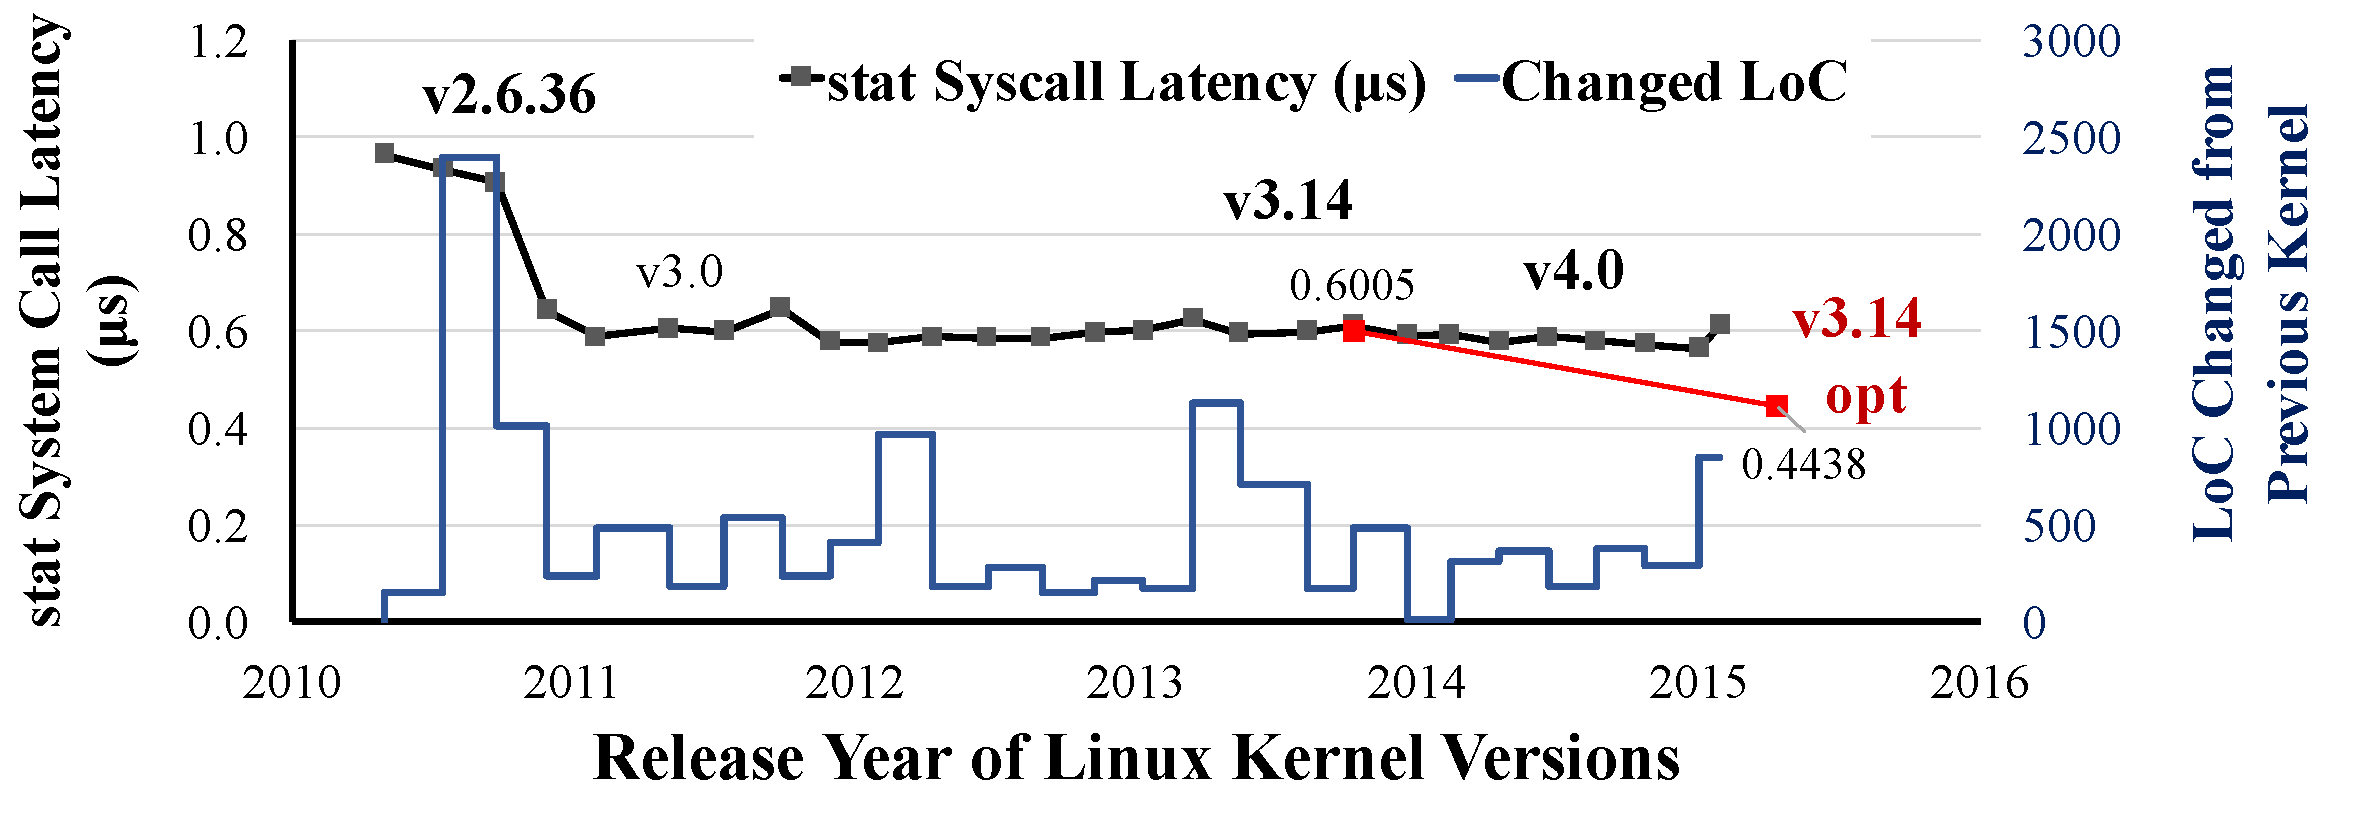
\includegraphics[width=6in]{dcache/plots/latency-by-version.pdf}
\footnotesize
\caption[Lantecy of {\tt stat} system call over years.]
{Latency of {\tt stat} system call with a long path {\tt XXX/YYY/ZZZ/AAA/BBB/CCC/DDD/FFF} on Linux over four years (lower is better), as well as the churn within the directory cache code (all insertions in {\tt dcache.c}, {\tt dcache.h}, {\tt namei.c}, {\tt namei.h} and {\tt namespace.c}). 
%Our optimizations significantly improve performance that has otherwise plateaued, despite significant ongoing developer effort.  
Our optimized \linuxver{} kernel 
further reduces {\tt stat} system call latency by \statspeedup{}\%.}
%\vspace{-15pt}
\label{fig:dcache:by-version}
\end{figure}


%\fixmedp{Add more evidence of lookup importance here: For instance, fraction of lookup time in file-related syscalls, or total lookup time in applications bound on file lookup latency.  }
Unfortunately, even directory cache hits are costly---0.3--1.1 \us{} for a {\tt stat} on our test Linux system, compared to only .04 $\mu$s for a {\tt getppid} and 0.3 \us{} for a 4 KB {\tt pread}. 
%\fixmetsai{Don, check this, I think read will be a better example, getppid is too trivial.}
This issue is taken particularly seriously in the Linux kernel community, which has 
made substantial revisions and increasingly elaborate optimizations to reduce the hit cost
of its directory cache, such as removing locks from the read path or replacing lock ordering with deadlock avoidance in a retry loop~\citep{corbet09jls,dcache-rcu}.
Figure~\ref{fig:dcache:by-version} plots directory cache hit latency against  lines of directory cache code changed 
over several versions of Linux, using a path-to-inode lookup \microbench{} on the test system described
in \S~\ref{sec:dcache:eval}.
These efforts have improved hit latency by 47\% from 2011 to 2013, but have plateaued
for the last three years.
%\fixmedp{if time, filter irrelevant changes from code deltas}
%at the cost of substantial developer effort.
%This latency appears to have plateaued 

The root of the problem is that the POSIX path permission semantics
seemingly require work that is linear in the number of path components,
and severely limit the kernel developer's implementation options.
%The root of this problem is that current directory cache
%designs reflect a straightforward implementation of the POSIX specification,
%which would seemingly require work that is linear in the number of path components.
For instance, in order to open file {\tt /\fnone{}/\fntwo{}/\fnthree{}} 
%for reading, 
one must have search permission
to parent directories {\tt /}, {\tt /\fnone{}}, and {\tt /\fnone{}/\fntwo{}},
as well as permission to access file {\tt \fnthree{}}.
The Linux implementation %of this specification is straightforward, 
simply walks the directory
tree top-down to check permissions.  
Unfortunately, when the critical path is dominated by 
walking a pointer-based data structure, 
including memory barriers on some architectures for multi-core consistency, 
modern CPUs end up stalling on hard-to-prefetch loads.
Moreover, because so many Linux features are built around this behavior, such as Linux Security Modules (LSMs)~\citep{wright+lsm},
namespaces, and mount aliases, it is not clear that any data-structural enhancements
are possible without breaking backward-compatibility with other Linux kernel features.
A priori, it is not obvious that a faster lookup algorithm, such as a single hash table lookup, 
can meet these API specifications and kernel-internal requirements; to our knowledge,
no one has tried previously.

%This paper proposes a decomposition of the directory cache, which allows
%most lookup operations to execute with a single hash table lookup (\S\ref{sec:dcache:dcache}),
%as well as optimizations to reduce the miss rate based on information that is {\em already in the cache}, but not used effectively (\S\ref{sec:dcache:readdir}).
%Our design maintains compatibility (\S\ref{sec:dcache:generalize}) through 
%several essential insights, including 
%how to separate the indexing of paths from checking parent permissions,
%and how to effectively and safely memoize the results of access control checks.


%% This paper proposes several new ways to organize a directory cache, which can yield 
%% substantial performance improvements over the current state of the art.
%% %This paper demonstrates that, despite this developer effort, there is still a substantial 
%% %missed opportunity hiding behind historical, intuitive, but not fundamental design choices.
%% Most of the Linux directory cache design reflects a straightforward implementation of the POSIX 
%% specification. %, with a division of labor that is suitable for mainstream file systems.

%This paper presents an alternative directory cache organization, which 
%improves performance by separating logical tasks, such as separating path indexing from permission checking; yet the design is sufficient to retain compatibility with POSIX.
%In the case of path lookup, 
%this paper demonstrates how 
%a per-component tree walk can be replaced with a single hash table lookup (\S\ref{sec:dcache:dcache}).
% without violating POSIX compliance.

%Our optimizations improve the performance of frequent lookup operations, but 
%introduce several costs, described in \S\ref{sec:dcache:dcache} and measured in \S\ref{sec:dcache:eval},
%which  we believe are acceptable and a net improvement for applications.
%First, these optimizations slow down infrequent modifications to the directory hierarchy, such as {\tt rename}, {\tt chmod},
% and {\tt chown} of a directory. 
%However, these slower operations
%account for less than .01\% of the system calls in the iBench traces~\citep{filenotafile}.
%Second,  the memory overheads of the dcache are increased.
%%(45\% per \dentry{}, as well as some  in our prototype).
%%(\fixmedp{XX MB} in our tests).  
%Third, lookup has a 
%probability of error from signature collisions that can be adjusted to be negligible
%%($2^{-141}$ in our configuration), 
%and within acceptable thresholds widely used by data deduplication systems~\citep{Debnath:2010:CSU:1855840.1855856, Srinivasan:2012:ILI:2208461.2208485, Quinlan:2002:VNA:645371.651321, Zhu:2008:ADB:1364813.1364831}.
%%, as well as how to remove
%%all memory barriers from the lookup path (\S\ref{sec:dcache:update}).
%In the micro-benchmark of Figure~\ref{fig:dcache:by-version}, our directory cache 
%optimizations improve lookup latency by 
%%revisions improve latency of accessing a long path
%%by 
%\statspeedup{}\% over unmodified Linux.
%%Our design addresses other missed
%%opportunities, such as identifying new opportunities to reduce the miss rate
%%through caching directory completeness.
%%\fixmedp{Do we want to highlight LoC?  3K is more than anything in the graph} \fixmetsai{Probably just mention in the evaluation. It's a metric that we should provide, but it's not awfully interesting.}
%%The total lines of code changed are fewer than 3,000 out of \fixmedp{XX}.
%%\fixmedp{Can we get 
%%, yet changes fewer than 3,000 lines of code.

%% SOSP cut - kind of long-winded
\begin{comment}
This paper rethinks current Linux directory cache design choices in light of the following goals:
\begin{compactitem}
\item {\bf Minimize the cost of a cache hit.} (\S\ref{sec:dcache:dcache}).
This means maximizing the benefit of temporal locality for frequent operations,
while pushing extra work of consistency maintenance onto less frequent, already-expensive operations.
%such as handling cache miss or updating massive metadata,
%in order to improve very frequent operations.
\item {\bf Maintain legacy compatibility.} (\S\ref{sec:dcache:generalize}).  Unix path semantics are complex, required by applications, file systems, and security modules, frustrating otherwise straightforward optimizations.  However tempting it may be to redesign path behavior to facilitate caching, path operations must exhibit the same behavior, with lower latency.
\item {\bf Never miss the same request twice in quick succession.} (\S\ref{sec:dcache:readdir}).  A number of less-frequent operations, such as reading a directory or secure temporary file creation, always miss in the cache {\em even if enough information is in cache to satisfy the operation.}  
%Of course, infrequent accesses should still be subject to a cache replacement policy, such as LRU.
\end{compactitem}
%Although directory caches must implement more complex semantics than a hardware memory cache,
%these principles should seem familiar to the reader with a basic architecture background.
%sadly, the Linux directory cache design violates all three.
\end{comment}

%This paper introduces several techniques to improve the performance of a directory cache,
%This paper explains several practical directory cache optimizations,
This paper demonstrates that these techniques improve performance for applications that use the directory cache heavily,
and the harm is minimal to applications that do not benefit.
%and that the worst case \microbench{} is only 12\% slower within \fixmedp{XX}\% of unmodified Linux.
%Each optimization we describe improves performance in isolation, and all can be combined.
%These optimizations change very few lines of code, and are backward-compatible with 
%legacy applications.  
%These changes are encapsulated in the VFS---individual file systems do not have to change their code.
%This paper describes a  prototype of these improvements implemented in Linux \linuxver{}.
%\S~\ref{sec:dcache:background} explains that the directory cache structure of Mac OS X, FreeBSD, and Solaris 
%are sufficiently similar that these principles should generalize.
%we compare and contrast Linux's directory cache
%with Mac OS X, FreeBSD, and Solaris in \S\ref{sec:dcache:background}, and explain inline how each
%optimization could be generalized to these other OS kernels.





%% \item {\bf Modularization and stackability}:
%% Any changes or optimizations must be implemented as modules inside Linux's VFS,
%% and can be stacked on top of the original design or any future optimizations. 
%% \item {\bf Backward compatibility}:
%% Any changes or optimizations must maintain least requirement of modifying any
%% file systems.
%% \item {\bf Generalization to other OSes}: Any changes or optimizations must be portable to other OSes with reasonable effort and change of design.




%% \dcache{} is proven to be effective on improving storage performance.
%% Experiments shows that,
%% in a Linux 3.x kernel, a \dcache{} with a xxx\% hit rate can speed up
%% metadata lookup and fetching time by xxx times.
%% \fixmetsai{experiment result, Linux version, and fs specs here}
%% However, we observed that Linux maintainers have made
%% constant and non-trivial efforts to improve \dcache{} in the Linux kernel.
%% We studied all \dcache{}-related source files in the Linux kernel Git repository,
%% and discovered that maintainers have committed
%% on average xxx revisions per source files.

%% We tested metadata lookup time on primary \dcache{}-related revisions.
%% Most changes on \dcache{} system only create xxx\%-xxx\% speed-up
%% than their predecessor.
%% \fixmetsai{result and graph here}.
%% Moreover, improvement to \dcache{} is still work-in-progress
%% for Linux maintainers.
%% \fixmetsai{reference to threads for latest dcache discussions}. 
%% All the evidences show that,
%% despite of significant reduction of storage operations,
%% efficiency of \dcache{} system internally still remains as a concern.

%% We argue that the design of \dcache{} needs to be carefully re-examined,
%% to fundamentally identify any missed opportunities that
%% improve value of \dcache{}.
%% At a high level, most optimization works for \dcache{} are focused on
%% improving ``how to cache'',
%% but we want to also lay eyes on ``what to cache'',
%% to ensure any valuable information returned from file systems
%% be captured by \dcache{} system.

%The contributions of this paper are as follows:
%\begin{compactitem}
%\item A performance analysis of the costs of path lookup and the opportunities
%to improve cache hit latency.
%\item A directory cache design that improves path lookup latency with a combination of techniques, including:
%  \begin{compactitem}
%  \item Indexing the directory cache by full path, reducing average-case lookup from linear to constant in the number of path components.
%  \item A Prefix Check Cache (PCC) that separates permission checking from path caching.  The PCC memoizes permission checks, and is compatible with LSMs~\citep{wright+lsm}.
%  \item Reducing the cost of checking for hash bucket collisions with path signatures.
%  \end{compactitem}
%\item Identifying opportunities to leverage metadata the kernel already has to reduce miss rates, such as tracking whether a directory is completely in cache.
%\item Carefully addressing numerous, subtle edge cases that would frustrate rote application of these techniques, such as integration with symbolic links and Linux namespaces.
%\item A thorough evaluation of these optimizations.  For instance, our optimizations improve throughput
%of the Dovecot IMAP server by up to \dovecotspeedup\% and latency of 
%updatedb by up to \updatedbspeedup{}\%.
%%git version control system by up to 25\%.
%
%\end{compactitem}

\papersection{\Thehostabi{}}
\label{sec:overview:host}

\issuedone{1.1.b}{Describe \thehostabi{} specification}
The development of \graphene{} starts with defining a simple host ABI (application binary interface) called \thehostabi{},
containing only OS abstractions essential to target applications.
%and is easily ported to different platforms.
%and minimal specifications for the host OSes and hardware.
%The host ABI is a new boundary between OSes (or hypervisors) and applications.
\Thehostabi{} separates
the implementation of an existing system API (application programming interfaces), which determines the compatibility against applications,
from hardware abstraction features, such as file systems, network stacks, and device drivers. 
\graphene{} moves the system API components
to a \libos{} in the userspace and reimplements the functionality using \thehostabi{}.
To port \graphene{} to a new host OS or hardware,
OS developers only have to implement \thehostabi{} on the target host system API,
%to new host OSes and hardware,
instead of paying a tremendous cost to translate the whole system API specification. Figure~\ref{fig:overview:porting} illustrates the porting process of \graphene{}.



%The host ABI separates the low-level, hardware management features, from the idiosyncrasy of system interface. 
%\graphene{} moves the upper layer of OS components,
%including the system calls and namespaces, into an library OS,
%leaving \thehostabi{} 
%as a narrowed interface to the host OSes and hardware.
%The host ABI intends to minimize the development effort on each host OS or hardware
%to mitigate the interface distinctions,
%to simply porting the OS abstractions defined in \thehostabi{}.


\begin{figure}[t!]
\centering
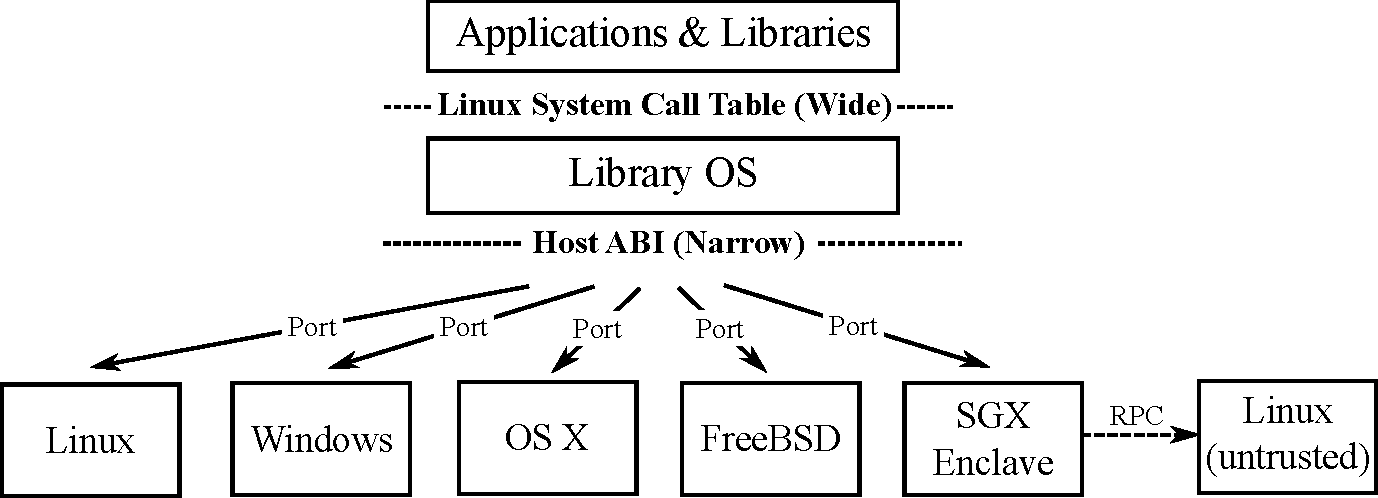
\includegraphics[width=30em]{porting.pdf}
\caption{Porting model of \graphene{}.}
%\vspace{-.1in}
\label{fig:overview:porting}
\end{figure}



\papersubsection{Platform Adaption Layers (PALs)}
\label{sec:overview:host:pal}


For each host OS or hardware, \graphene{} uses
a thin library called a {\bf platform translation layer (PAL)}
to translate among host interfaces.
%is loaded below the library OS, to translate each functions in \thehostabi{} to native system interfaces.
The main purpose of a PAL is to mitigate the semantic gap
between \thehostabi{} and
native host system APIs.
%The effort of PAL development is per host OS, whereas the library OS implementation is reusable on every hosts. %The simplicity of \thehostabi{} can be also estimated by the effort of implementing a PAL for each host.
By implementing a PAL on a new host OS or hardware,
users can reuse
the same \libos{} to run the same collection of unmodified Linux applications.
%To keep the porting effort low,
%the development of a PAL must be straightforward
%for average OS developers.
%to achieve with limited efforts.
%Based on the principle of porting simplicity, PAL development must be straightforward
%for average developers.







%The host ABI is defined for the simplicity of porting, as well as the sufficiency for implementing a library OS compatible to Linux.
%First of all, the number of host functions included in \thehostabi{}
%is much smaller than the number of system calls in a commodity OS such as Linux. 
\graphene{} currently contains PAL implementations for several popular OSes,
including Linux, \win{}, \osx{}, and FreeBSD.
%and \sgx{} with an untrusted Linux kernel.
Most of these OSes provide a POSIX-like system API similar to \thehostabi{}.
Due to the similarity, translating most of \thehostabi{} to one of the system APIs
are straightforward for average OS developers.
\Thehostabi{} is also much smaller than the actual POSIX API, making it extremely portable.



A part of \thehostabi{} may be challenging to port
on an OS,
due to unexpected system assumptions made by the OS.
For instance, \win{} does not support
fine-grained memory deallocation for de-privileged applications.
To implement system calls like \syscall{munmap} and \syscall{mprotect},
\graphene{} needs host ABIs to
deallocate or protect virtual memory pages at page granularity.
%A workaround is to change memory mappings at the physical page level,
%but will require running the \win{} PAL with root permissions.
%This type of porting challenges
%tends to be results of design decisions or assumptions made by OS developers.
%A \libos{} can potentially design
%different emulation strategies
%to compensate missing host abstractions.
A few host abstractions such as a bulk IPC feature are
optional to the host ABI;
if a host OS does not support these abstractions,
the \libos{} must fall back to alternatives. 

%In our experience, the development of a PAL is around ten thousand lines of code.

%For each port, the amount of code written for implementing \thehostabi{} is at the order of magnitude of thousands of lines of code, which is much more manageable than implementing a flat translation layer for system interfaces.


\begin{comment}
Based on the experience in \graphene{},
it is hard to ensure the portability of \thehostabi{} on every potential hosts.
%even a host ABI specialized for simplicity cannot guarantee to be portable on every hosts.
A host may simply lacks the functionality
for implementing a \hostapi{}.
The assumption is, maintaining the compatibility of \thehostabi{} poses a much less challenge than maintaining the whole system API.
Besides, the library OS may flexibly switch among emulation strategies
to compensate the absence of certain host abstraction.
As an example,
bulk IPC is optional in \thehostabi{} since its first definition,
due to the expectation
that implementing the feature may not be feasible on some hosts.
If bulk IPC is not available,
the library OS can fall back to RPC-based IPC, with a reasonable amount of performance penalty.
In the worst case, if there is no emulation strategies
to compensate for the absence of a \hostapi{},
user can predict the affected applications and avoid running these applications
on specific hosts. 
%at least users can predict whether an application will be affected and thus cannot run on certain hosts.
\end{comment}


%For a host OS that does not support ELF binaries, the PAL must follow the binary format which the host OS accepts, such as the Portable Executable (PE) format on \win{}.
%The PAL is the only layer in the user space which cannot be reused
%across different hosts. Besides the PAL, all of the other binaries in the user space are fully reusable, including the library OS, the supporting libraries, and the application executable.



%The host abstractions map to several common system calls in a commodity OS.
%For example, \funcname{StreamRead} and \funcname{StreamWrite} can directly map to the POSIX functions \funcname{pread} and \funcname{pwrite}, which are available in most OSes including Linux, BSD, \osx{}, and \win{}.
%More than half of the functions in \thehostabi{} can be counted toward this category.
%The rest of the host abstractions are either specific to Linux
%(e.g., TLS support),
%or belong to the POSIX functions that are not shared with commodity OSes
%(e.g., \funcname{mmap} on \win{}).
%The PAL emulates these host abstractions, using existing system interfaces available on the host OS, unless the software emulation is fundamentally impossible (e.g., restricted by the system interfaces), or too expensive (e.g., high overhead from copying data).



\papersubsection{Definitions and design principles}
 

\graphene{} defines \palcallnum{} calls in \thehostabi{} (also called \hostapis{}),
with a set of host abstractions
sufficient for \libos{} development.
%The host ABI defines the interaction between the library OS and a specific host.
%The \graphene{} library OS can be deployed on any ``host'' where \thehostabi{} has been ported.
This thesis defines
a {\bf host} of \thehostabi{}
to be an OS or hypervisor
which contains enough OS functionality for running a standalone application or virtual machine.
Most of the host targets in \graphene{}
are monolithic OSes,
including Linux, \win{}, \osx{}, and FreeBSD.
%which has defined a massive system API for programmability.
A monolithic OS 
usually contains a massive amount of system APIs,
which is sufficient for
implementing \thehostabi{}.


A special example of a host
is an \sgx{} (Software Guard Extensions) enclaves~\cite{intelsgx},
which
restricts OS functionality for security reasons.
The restrictions on \sgx{}
are results of a strong threat model
which distrusts any OS features except ones that are virtualized by the CPUs or migrated into enclaves.
The only way to obtain any missing OS features such as storage or networking
is to request through RPC (remote procedure call).
Requesting untrusted OS services through RPC also introduces new security threats that application developers tend not to anticipate~\cite{checkoway13iago,osdi16scone}.
Due to all the compatibility and security challenges discussed above,
this thesis uses \sgx{} as a representative example of a host
with unusual assumptions (e.g., threat models) and restrictions
compared to a monolithic OS.

%An innovative hardware abstraction like \sgx{} (software guard extensions)
%imposes unique assumptions and restrictions
%on a commodity OS,
%%creates a special host on top of Linux or \win{},
%%with unique interfaces and specifications regarding the host OSes.
%and thus creates a special host above the OS.

%If an OS has mutated or tweaked the interface for a hardware platform,
%such as an \sgx{} enclave 
%running on an untrusted Linux kernel,
%the combination of the OS (Linux) and the hardware platform (\sgx{}) is considered a specialized host.
%Especially, the \sgx{} port of \thehostabi{} faces several unique challenges,
%which will be discussed in Chapter~\ref{chap:sgx}.


\begin{comment}
%\fixme{each sentense should be a paragraph; starting the 2nd sentence}
\fixmedp{start with a strong opening stating the rationale}
The host ABI of \graphene{}
define functions needed from a host, in order to implement the library OS for reusing applications.
%to reuse an application and all its supporting libraries, including the \graphene{} library OS.
Each host of \graphene{} contains an OS and a hardware platform, either of which causes compatibility issues for running unmodified applications.
OS developers can port the library OS to a new host,
by simply reimplementing the narrowed host ABIs using abstractions available on the host.
%a new host platform.
%For each host which requires the compatibility for unmodified Linux applications, one only has to implement the narrowed host ABIs,
%instead of reimplementing the bloated, ``legacy'' system interfaces
%needed by the applications.
By implementing \thehostabi{}, OS developers skip the painful process of rebuilding the whole system interfaces of a commercial OS such as Linux.
The host ABIs strictly decouples the porting effort on the hosts from the compatibility feature for applications.
%The host ABIs decouple the OS development in the host and the implementation of compatibility for the existing Linux application.
What \thehostabi{} exposes is a simplified extended machine,
similar to a para-virtualization interface, capable of running the library OS as a lightweight virtual machine. % with compatibility against Linux applications.
%on which another layer of virtualization (i.e., the library OS) can be built to reproduce the compatibility for Linux.
\end{comment}


\begin{comment}
Two design principles drive the definition of \thehostabi{}s:
{\em simplicity} (i.e., easy to port on any hosts)
and {\em sufficiency} (i.e., containing enough OS functions for implementing a library OS).
The process of deciding \thehostabi{}s is comparable to
finding a ``pinch point'' within a OS implementation,
which can conveniently mediate a significant portion of OS execution paths for managing hardware abstractions.
%The two principles drive the development of \thehostabi{}s,
%The whole development of the \graphene{} library
%must be disciplined
%on extending \thehostabi{}s only when it is strongly required.
%of restraining extensions to \thehostabi{}s unless absolutely necessary.
The two principles
determine the soundness of the \graphene{} approach to improving compatibility
for any hosts.
\end{comment}


%%The host ABI is defined with partitioning in mind.
%\Thehostabi{} 
%determines a boundary which partitions several upper-level OS components, %, such as system calls and namespaces,
%into a library OS,
%%, as a dynamically-linked library which can be deployed
%%to various hosts.
%%The rationale behind the partitioning is based on the fact that not every OS component is equally important to compatibility, for applications which need to be ported across hosts.
%%When an OS is extended for a new hardware,
%%these OS components usually remain unchanged, or are predominantly reused.
%%Partitioning
%%into a library OS further guards these 
%in order to isolate the host idiosyncrasy. % on specific hardware. %any potential changes for adopting new hardware.
%%Similar isolation
%%exists in traditional OSes, but without partitioning:
%The strategy
%is also used in OSes:
%An example is the Linux virtual file system (VFS), an internal interface
%which encapsulates operations of file system drivers.
%%On the other hand,
%%drivers (e.g., drivers for file systems, block devices, or network cards)
%%and architecture-specific instructions
%%stay encapsulated in the host OS.
%%in the Linux kernels are usually encapsulated under a virtualized, in-kernel interface (e.g., the Linux virtual file system),
%%to simplify the development of the rest of the kernel.
%Similar to VFS,
%\thehostabi{} is intended
%to be a more ubiquitous interface,
%which encapsulates
%any host-specific behavior and semantic
%inside the host OS.
%%for encapsulating both OS and hardware idiosyncrasy on a wide range on hosts.
%%declares a ubiquitous system interface, to encapsulate both OS and hardware abstractions
%%for the library OS.




\Thehostabi{} shares several characteristics with a virtual hardware interface
exported by a hypervisor.
A generic, backward-compatible
virtual hardware interface
%a set of generic, virtual hardware,
%which the VM can control with the same drivers.
allows an unmodified OS kernel to run inside a virtual machine as on the bare metal.
%by exporting interfaces close to commodity hardware.
%To avoid additional porting effort, the virtual hardware are close to the typical commodity hardware.
%For instance, a virtual hardware interface
%usually includes a virtual NIC (network interface controller),
%such as the virtualized E1000 interfaces
%available in VMware workstation or QEMU.
%As a result, \thehostabi{} contains the
%typical OS features and interfaces, similar to the API of early UNIX systems.
The key difference between
a virtual hardware interface
and \thehostabi{}
is that \thehostabi{} does not target reusing a whole, unmodified OS kernel as a guest.
Instead, 
\thehostabi{} contains higher-level abstractions such as files and network sockets
to ensure portability on most host OSes.
The concept
of defining \thehostabi{}
with a customized guest OS (i.e., a \libos{}) running atop \thehostabi{} is similar to para-virtualization.
%\thehostabi{} expects the \libos{}
%to be rewritten and
%customized for \thehostabi{},
%similar to a 
%para-virtualizated VM.
%Compared to an actual para-virtualized VM,
A para-virtualized VM defines hypercalls as interfaces between a guest OS and a hypervisor.
Furthermore, \thehostabi{} avoids duplication of OS components
such as scheduler, page fault handler, file systems, and network stacks
between the host and \libos{}.
%Another difference is that \thehostabi{} is called by normal function calls, whereas para-virtualization relies on hypercalls.
To compare a VM and a \libos{} on a spectrum,
a VM reuses a whole OS on a wide, backward-compatible virtual hardware interface
whereas a \libos{} implements only system API components on a simplified host ABI.

The following paragraphs discuss the key design principles of \thehostabi{},
including porting simplicity, sufficiency for \libos{} development, and ease of migration.

\paragraph{Porting simplicity.}
%To reduce porting effort
%\thehostabi{}
%must be simple to port on a host OS or hardware.
To reduce porting efforts,
\graphene{} defines \thehostabi{}
using two strategies:
first, \graphene{} significantly reduces both the size and complexity of host OS features
that OS developers have to implement.
Effectively, \graphene{} avoids duplicated OS features and handling rare corner cases
on \thehostabi{}.
%The development of \graphene{} disciplinarily avoiding adding any functions to \thehostabi{},
%unless the library OS cannot internally implement an OS feature.
Second, the definition of \thehostabi{}
imitates common system APIs in a POSIX-like monolithic OS,
to directly translate most calls to
a few similar host abstractions.
%existing system calls or system library functions
%on each host.
%include functions which can be directly mapped to OS functions exported by the host.
%%the likelihood of finding similar features on the host, to be translated to functions in \thehostabi{}.
%The assumption that such a strategy is possible
%is based on
%the observation that
%%similarity of system interfaces is common among most OSes.
%similar OS functions, especially UNIX-style APIs,
%tend to commonly exist in most OSes.
%, to reduce the learning curve for programming applications.
For instance,
the stream APIs in \thehostabi{}, such as \palcall{StreamRead} and \palcall{StreamWrite}
are similar to
system calls like \syscall{read} and \syscall{write} exist on Linux, BSD, and POSIX API,
or \syscall{ReadFile} and \syscall{WriteFile}
on \win{}.
%with similar functionality and semantics.
%and 
%looks similar to \syscall{ReadFile} in \win{}, except the data types.
%The definition of \thehostabi{}
%is based on observations of the system interfaces in some of the important hosts,
%including Linux system calls and \win{} API.
%exported by the targeted hosts,
%and defines the functions in \thehostabi{}, to be easily translated to the native system interfaces.
%The host ABI is essentially a subset of the common features from every potential hosts.
%We expect %\thehostabi{} defined with simplicity in mind
%to be straightforward to port on most hosts,
%Most functions in \thehostabi{} can be easily translated to host system interfaces
%in various styles.
As the rest of this thesis proves, porting \thehostabi{} is straightforward
on most monolithic OSes.

%For example, \thehostabi{} defines \syscall{StreamRead} and \syscall{StreamWrite} for accessing I/O streams, similar to .
%xcept some nuanced details like order of parameters.


% by including OS functions , such as \syscall{FileRead} and \syscall{FileWrite}, similar to the Linux system calls, \syscall{pread} and \syscall{pwrite}.




\begin{comment}
The simplicity of \thehostabi{}s requires retaining a minimalist design of host functions. %, based on typical OS services for managing hardware.
%\graphene{} reduces the host functions
%to the bare minimum.
The host ABIs should only contain operations that
are absolutely necessary for requesting external hardware abstractions.
%A way to simplify \thehostabi{}s is to move host functions into the library OS
%and to replace them with wrappers consisting of other host functions.
Any functions that can be partially or wholly implemented inside the library OS
should be further simplified, or even removed from \thehostabi{}s.
%---in other words, whether \thehostabi{}s can be further reduced.
Moreover, \thehostabi{}s have to be simple enough to implement on
most hosts;
%In the simplest host ABIs, none of the host functions shall be able to internally implement the behavior of another host function,
%or the definition of \thehostabi{}s is further reducible.
that is, \thehostabi{}s should contain only OS functions that are commonly offered on
most hosts.
The host ABIs are close to simplified UNIX interfaces,
such as reading or writing a file or an I/O device as a byte stream,
or creating a virtual memory mapping.
%the most common OS functions
%offered on most of the potential hosts,
For most hosts,
implementing \thehostabi{} should be as straightforward as redirecting the functions to the closest host system calls.
%such as the Linux system calls or the \win{} APIs.
For example, the functionality of \syscall{StreamRead} and \syscall{StreamWrite} in \thehostabi{}s can loosely match with
\syscall{read} and \syscall{write} in Linux,
or \syscall{ReadFile} and \syscall{WriteFile} in \win{}.
%This thesis also evaluates the simplicity of \thehostabi{}s by counting the lines of code used to implement \thehostabi{}s on each host platforms.
Since most OSes have inherited a similar design from UNIX,
it is fair to assume finding
comparable OS functions %host platforms
to \thehostabi{} would be reasonably easy.
%fair to assume that \thehostabi{}s 
\end{comment}



\paragraph{Sufficiency for \libos{} development.}
%\Thehostabi{} defines
%the host abstraction available for a \libos{} to access host hardware abstractions.
To develop a \libos{} with compatibility against a wide range of applications,
\thehostabi{}
%are demonstrated by the fact that
%the exported host functions 
contain any OS abstractions that the \libos{} cannot easily emulate.
%and a full-function library OS is implemented on top of them.
For most hosts,
the host OS abstractions
%can be categorized into five types:
include
process creation, memory management, and I/O (typically, files and network connection)~\cite{dhamdhere2007os-textbook}.
%Besides security and protection,
%the definition of \thehostabi{} is closely related with hardware management,
%and offers the most basic abstractions for each category of OS functions.
%managing specific types of hardware,
%and each contain a few basic abstractions
%which can be expanded into other system interfaces.
%For example, the basic OS functions for memory management include
%allocating (\syscall{VirtMemAlloc}),
%protecting (\syscall{VirtMemProt}),
%and deallocating (\syscall{VirtMemFree}) memory regions. % at certain granularity
%(usually in pages).
%These basic functions can be used to implement other forms of memory allocation,
%such as growing heaps with \syscall{brk}
%or allocating thread-private stacks.
%The definition of the \drawbridge{} host ABI is a hint, for creating a list of host abstractions necessary for the library OS, including streams, memory, threads, and processes. 
%If \thehostabi{}s are insufficient for implementing certain system interfaces, one may extend \thehostabi{}s with the missing functions,
%with the discipline to retain the simplicity of \thehostabi{}s.
%The extension to \thehostabi{}s must be d, to keep the extension minimal, and to avoid adding redundant functions.
%The implementation of the \graphene{} library OS demonstrates that
%\thehostabi{} is sufficient for implementing significant portion of Linux system calls.
For each type of abstractions,
a monolithic OS may define several variants of system APIs with similar functionality.
For instance, Linux provides two system calls, \syscall{mmap} and \syscall{brk}, both for memory allocation in a process.
\syscall{mmap} allocates larger memory regions with page granularity,
whereas \syscall{brk} simply grows a single, continuous heap space for more fine-grained allocation.
Many applications such as GCC~\cite{gcc}
switch among system API variants in case one of them is unavailable on certain OS distributions.
This thesis shows that,
by adopting only the semantics of one of these similar APIs or abstractions, the host OS can stay simple with
the \libos{} emulating the rest of APIs.
For instance, \thehostabi{} includes \syscall{VirtMemAlloc}
as a similar feature as \syscall{mmap},
which is sufficient to emulating both \syscall{mmap} and \syscall{brk}.



\graphene{} defines \thehostabi{} partially based on
\drawbridge{},
a library OS for single-process \win{} applications.
The host ABI of \drawbridge{} 
contains 36 functions,
%demonstrates that its host ABI is sufficient
%for running a library OS in which 99.7\% of code comes from the \win{} 7 source.
%The host ABIs of \drawbridge{} are later extended
%for running a Linux-based library OS called Bascule~\cite{baumann13bascule}.
and several works have ported the host ABI to different hosts,
including \win{}, Linux, Barrelfish, and \sgx{}~\cite{porter11drawbridge,baumann14haven,mssql-on-linux,baumann13bascule}.
%and is capable of running a library OS for single-process, Linux applications, with a few host ABI changes~\cite{baumann13bascule}.
%ill loads and links the rest of application binaries, just like the native Linux loader (i.e., \code{ld.so}).
%\graphene{} takes the high-level definitions of the \drawbridge{} and Bascule host ABIs, and customizes for general-purpose Linux applications and a wider range of hosts. 
Although running \win{} and Linux applications may face
a different set of challenges,
the nature of their APIs is mostly similar, with a few exceptions.
During the development of \graphene{}, developers found the occasions in which
the host ABI of \drawbridge{}
is not sufficient to address Linux-specific challenges
and decide to extend \thehostabi{}.
Section~\ref{sec:overview:host:abi} and Chapter~\ref{chap:abi}
will further discuss the Linux-specific extensions of \thehostabi{}.


\paragraph{Migration.}
The \graphene{} library OS shares several features of VMs, including checkpointing and migrating a running application.
Migrating a process is also the key to emulating copy-on-write forking,
on a host without physical memory sharing (e.g., \sgx{}).
A hypervisor checkpoints and migrates a VM by snapshotting the VM states above a stateless virtual hardware interface. % as a clean boundary for snapshotting the application and OS state.
\Thehostabi{} is also defined to be statelessness,
by ensuring any states in the hosts to be temporary and reproducible to the applications and \libos{}.





\papersubsection{The \hostapis{}}
\label{sec:overview:host:abi}


%\fixmedp{the beginning doesn't capture the whole paragraph.}
%The host ABI shares several common abstractions with production OSes.
%The functions in \thehostabi{}
%define the basic features needed from the hosts, to run the library OS.
%The definition of the host functions
%should be unsurprising to average OS developers,
%making the implementation on a new host to be fairly straightforward.
%The host ABI reflects the common functionality of most OSes, including Linux and \win{}.
%Although the same OS abstractions may be defined
%as different idiosyncratic system interfaces on each host OSes,
%\graphene{} takes into consideration of porting the host functions to either OSes, in the most effortless way possible.





%fixmedp{give more of the background}
Table~\ref{tab:overview:abi} lists the \palcallnum{} calls defined in \thehostabi{}:
%Among these \hostapis{}, 
25 calls are inherited from the \drawbridge{} host ABI,
including functions to managing I/O (e.g., \palcall{StreamOpen}), memory allocation (e.g., \palcall{VirtMemAlloc}), scheduling (e.g., \palcall{ThreadCreate}), and several miscellaneous functions (e.g., \palcall{SystemTimeQuery}).
%Most of the host functions only affect the OS or hardware states
%related to the process itself.
%For example, \syscall{VirtMemAlloc} can only allocate memory in the calling process,
%and cannot affect other processes running in parallel.
%Only I/O streaming functions export states to the host OS, and share states with other processes or library OSes.
14 calls are added by \graphene{}, to implement Linux-specific features.
For example, unlike \win{} or \osx{}, Linux %The host ABI is also complemented with several Linux-specific abstractions, such as
delivers hardware exceptions to a process as signals.
Linux also requires 
the x86-specific segment registers (i.e., FS/GS registers)
to determine the location of thread-local storage (TLS), which can be hard-coded in application binaries by a compilation mode of GCC.
On \win{} or \osx{}, the x86-specific segment registers are mostly ignored, and even frequently reset to eliminate attack vectors.
%The host ABI contains host functions (), which can be directly called from the library OS. \graphene{} shows that \thehostabi{} is sufficient to implementing a large portion of the Linux system calls.
%These functions are not defined in \drawbridge{}, the \win{}-based library OS,
%because these abstractions do not exist in \win{}.
%The \drawbridge{} host ABI does not contain exception delivery because the feature is
%not commonly used in \win{} applications.
%Moreover, the x86 segment registers cannot be modified in \win{}
%because the OS assigns fixed values to these registers
%for the whole execution.
%Although \drawbridge{} excludes these abstractions, Bascule extends \thehostabi{} to include similar functions,
%demonstrating that the extension is indeed necessary.
\graphene{} discovers these abstractions as a necessity for implementing a rich Linux \libos{}.



\begin{table}[htp!]
\centering
\input{abi-table}
\caption{An overview of \thehostabi{} of \graphene{}. The ones marked with the symbol $\dagger$ are introduced in the initial publication of \graphene{}~\cite{tsai14graphene} or later extended for this thesis. The rest are inherited from \drawbridge{}~\cite{porter11drawbridge}.}
\label{tab:overview:abi}
\end{table}

%The interfaces, as part of \thehostabi{}, which access these host abstractions, are ultimately simplified to reduce the porting effort on each host.
%Unlike the system interfaces in the OS, \thehostabi{} does not prioritize backward compatibility. Therefore, \thehostabi{} includes only the minimum interfaces that the library OS needs to interact with the host. The host ABI does not have to include any of  the legacy system interfaces from a production OS, let alone preserving different flavors of system interfaces for backward compatibility.



\graphene{} introduces five calls for 
remote procedure call (RPC) between \libos{} instances
in a multi-process application.
\graphene{} simplifies porting multi-process abstractions
on each host OS
to implementing RPCs.
The basic RPC abstraction is 
a pipe-like RPC stream for message passing between processes.
To improve performance,
%RPC is critical for implementing the coordination of OS states
%across library OS instances.
%The basic form of RPC in \graphene{} is a pipe-like RPC byte stream, which a library OS can simply use to send messages.
%It is a common design choice
%to implement inter-process coordination through message-passing
%instead of shared memory, especially for hardware platforms that do not guarantee memory coherence~\cite{baumann09barrelfish}.
%A problem to the message-passing approach is the significant overheads
%on frequently exchanging distributed OS states.
\thehostabi{} defines an optional, bulk IPC abstraction
to send large chunks of virtual memory
across processes.
%The bulk IPC feature works similarly as sending the memory through RPC streams,
%but is much faster because it avoids copying memory in the host.


%for host platforms that urgently require lowering the RPC overheads.
%Another extension is for
%%\funcname{StreamSendHandle} and \funcname{StreamRecvHandle}
%delegating opened stream handles to another process, through a connecting pipe.
%The feature is similar to sending file descriptors
%through UNIX sockets in Linux, and is used to share opened network sockets with the \syscall{fork}'ed processes.
%%Another RPC abstraction is a bulk IPC channel; a process can use \funcname{PhsyicalMemoryCommit} to commit a large chunk of memory to a bulk IPC channel, which \funcname{PhsyicalMemoryMap} can map into another process, as copy-on-write. The library OS uses bulk IPC as an optimization to \syscall{fork}.
%Despite that either of the RPC primitives
%is not necessary easy to implement on every hosts, the inclusion of these host functions is completely optional, and the library OS can always fall back to the message-passing approach.



%All the host functions are designed to appear as ``stateless''
%as possible to the library OS.
%Being stateless to the library OS means that
%a host function does not preserve any permanent state of certain host abstraction.
%A stateless function can recover
%from disconnection of the library OS, and be reconnected at any timing.
%The host functions can maintain temporary bookkeeping for the convenience of porting,
%but should not assume the bookkeeping states to be permanent.
%The principle of defining all the host functions to be stateless
%is primarily for two purposes:
%{\em migration} and {\em security isolation}.
%For migration, the fact that the library OS can disconnect freely from the host functions simplifies the implementation of the migration feature.
%Migration is also an important foundation to implementing \syscall{fork}, because the cloned process need to receive a snapshot of the parent process.
%For security isolation, 
%a stateless host function is easier to check,
%because the security monitor only has to verify each instance of host function calls,
%instead of tracing multiple host functions over a longer period of time.

%the functions to access each host abstraction must appear \fixmedp{clarify `stateless'} stateless to the host, except for the handles to identify the resources. Each call to the host functions is independent. The arguments given for each call must be always be absolute values, instead of relative values.
%For example, the offset given to \funcname{StreamMap}, \funcname{StreamRead}, and \funcname{StreamWrite} (if the opened handle is a file) are offsets from the beginning of the file, and thus are irrelevant to how many bytes that are previously written or read.
%When enforcing isolation rules, the host OS can check the arguments of each calls to the host functions, independently and atomically.


%A host ABI (application binary interface) has to define the convention of application binaries, including the binary format and the linking procedure, as well as a set of  system interfaces.
%The host ABIs contain a minimal loader which recognizes a basic version of the ELF (Executable and Linkable Format), just enough to compose a binary of the library OS.
%The very initial loading procedure as part of \thehostabi{}s only loads a clean library OS instance.
%Each host of \graphene{} is supposed implement a minimal dynamic loader,
%which can load the \graphene{} library OS binary in ELF.
%The library OS then completes the dynamic loading procedure,
%by directly loading the Linux native dynamic loader (i.e., \code{ld.so}), and indirectly loading the rest of the application binaries.







\papersubsection{Host-enforced security isolation}
\label{sec:overview:host:security}


To target multi-tenant environments, 
\graphene{} enforces strong security isolation between mutually-untrusting applications running on the same host.
The security isolation of \graphene{} is comparable to running each application
in a VM or a container.
Just as a virtual hardware interface isolating each VM,
\thehostabi{} also enforces security isolation between library OS instances.
%according to the trust model of the applications.


On a trusted host OS,
\graphene{} delegates security isolation as a host-level feature.
The library OS and the application must mutually trust each other, due to lack of internal privilege separation in a process.
%The host ABI also separates API implementation
%from security isolation.
%To ensure isolation, each host must restrict access from the applications or the library OS, to any unauthorized host abstractions.
On each host, a reference monitor enforces security isolation policies, by access control on OS abstractions sharable among processes, including files, network sockets, and RPC streams.
%The host-level security isolation is orthogonal to API complexity.
Separating security isolation from API implementation simplifies security checks
for applications that only require
complete protection from other tenants.
%based on monitoring the references to host resources and rejecting authorized resource access.
%to the host abstractions.





%\graphene{} reduces the attack surface exposed to applications
%by restricting access to the host kernel ABI 
%and prevents access to unauthorized system calls, files, byte streams,
%and network addresses with a \emph{reference monitor}.
%The host kernel ABI exported by the \pal{} heavily 
%limits the ability of a \graphene{} application to interact with the rest of the system;
%any external interactions are further mediated by a reference monitor.
%Unlike a typical Linux system, \graphene{} applications cannot interact with shared 
%system daemons or other shared system resources.
%As a result, \graphene{} enforces security isolation similar to running applications in separate VMs---even
%applications that span multiple processes.


In \graphene{},
one or multiple processes of the same application run in a {\bf sandbox}.
Multiple library OS instances coordinate
in a sandbox
to present a unified OS view
to the application.
%As the library OS instances can coordinate shared OS states using simple RPC streams,
The design simplifies the enforcement of security isolation for multi-process abstractions.
\graphene{}
uses the reference monitor to block RPC streams across the sandbox boundary,
stopping applications in different sandboxes from accessing multi-process OS states.
%\graphene{} contributes a multi-process security model 
%based on the abstraction of a \emph{sandbox},
%or a set of mutually trusting processes.
%If a reference monitor exists, the reference monitor permits the processes within the same sandbox to communicate and exchange RPC messages, but disallows cross-sandbox communication.
The current design focuses on security isolation, although we do expect to extend the design for more sophisticated policies
in the future.

\begin{comment}
The only host abstractions that are shared across processes and must be mediated by the host for isolation are files, network sockets, and RPC streams
--- all other allowed host ABI modify only local process state, such as VMAs and threads.
%Thus, the reference monitor need only mediate file access, socket and RPC stream creation.
%an unprivileged daemon
%as well as extensions to the App\-Armor LSM~\cite{apparmor},
%which checks file and socket policies in the kernel.
%, reducing context switching overhead
%and the risk of race conditions~\cite{garfinkel03traps}.
In order for the reference monitor to restrict file access, socket and RPC stream creation,
each application includes a {\em manifest file}~\cite{hunt07rethink},
which describes a {\tt chroot}-like, restricted view of the local 
file system (similar to Plan 9's unioned file system views~\cite{pike90plan9}),
%including read-only shared files,
as well as {\em iptables}-style~\cite{iptablesman} network firewall rules.
To facilitate sharing read-only libraries, a manifest may specify a file system view which combines several different sub-directories of the local file system, and can prevent writing to files or directories.


For example, the \graphene{} reference monitor on the Linux host is implemented using \syscall{ioctl} to a special device (\code{/dev/graphene})~\fixme{a prospective design}.
A process is restricted by the Linux BPF-style system call filter, or the SECCOMP filter~\cite{seccomp}, to use \syscall{open} to access any files, or to \syscall{connect} or \syscall{bind} to any sockets.
It must use the \graphene{} special device to open or create streams, so the file paths or network addresses can be checked against the sandbox rules. The kernel module as the driver of the \graphene{} special device can coexist with any Linux Security Module (LSM), such as AppArmor~\cite{apparmor} or SELinux~\cite{selinux}.


When a new process is launched by the host, it begins execution in a new sandbox.  
Child processes may either inherit their parent's sandbox, or can be started in a separate sandbox---specified by a flag to the host abstractions of process creation.
A parent may specify a subset of its own file system view 
when creating a child, but may not request access to new regions of the host file system. 
%The restrictive policy enforced on the child will be written in a new manifest file generated by the parent, and the policy will be checked by the reference monitor.
The child may also issue an {\tt ioctl} call to 
dynamically detach from the parent's sandbox. The reference monitor prevents byte stream creation across sandboxes.
%among picoprocesses
%that are not in the same sandbox.
%and restricts external connections to remote URIs according to firewall rules in the manifest.
When a process detaches from a sandbox, effectively splitting the sandbox, the host must closes all RPC streams that could bridge the two sandboxes.
\end{comment}



\paragraph{Threat model.}
For most hosts, application trusts the host OSes as well a \libos{} instances in the same processes.
For multiple processes inside a sandbox,
the \liboses{} in these processes
also trust each other.
Applications or \liboses{} are not trusted by the host OSes or processes outside of the sandboxes.
Applications and \liboses{}
can become the adversary to the host OS,
by exploiting vulnerabilities on \thehostabi{}.
%the \graphene{} design reduces the attack surface between the hosts and the library OS instances, to defend against a malicious application.

%On a host with a reference monitor, the host OS and the reference monitor are both trusted, to mediate all system interfaces used to implement \thehostabi{}. The host must check all access to any abstractions with effects outside of a process's internal state, such as an opened file, or a connected network socket.
%Processes inside the same sandbox mutually trust each other. The adversary can run arbitrary code inside of one or more processes within one or more sandboxes.
%The adversary can control all code in its processes, including the library OS and the host-specific PAL.
%{\tt libLinux} and the \pal{}. 
%We also assume a trusted reference monitor process running on the host kernel that 
%launches \graphene{} applications and mediates all system calls with external effects,\fixmedp{define precisely}

%\graphene{} ensures that %The key security property the \graphene{} design upholds is that 
%the adversary cannot interfere with any victim picoprocesses
%in a separate sandbox.  
%The \graphene{} sandbox design ensures strict isolation: 
%if the only shared kernel abstractions are byte streams and files, 
%and the reference monitor ensures
%there is no writable intersection between sandboxes,
%the adversary cannot interfere with any victim picoprocess.


The threat model of \graphene{} on \sgx{}
contains the adversary from other hosts but excludes
the host OS, hypervisor, and any hardware except the CPU from its trusted computing base (TCB).
An untrusted OS or hypervisor
potentially has lots of opportunities to invade applications or VMs,
using Iago attacks~\cite{checkoway13iago}.
The challenges of porting \graphene{} to \sgx{} is not limited to resolving the compatibility issues of enclaves but also defending applications and \liboses{} against untrusted host OSes.







%%% The only processes allowed to run as standard kernel processes (non-\graphene{}) 
%%% are the reference monitor and
%%% system administration utilities that need more kernel interfaces than the \pal{} ABI provides.
%%% Ensuring that a collaborating picoprocess correctly implements
%%% some function (such as receiving a signal),
%%% as well as preventing exploitation of vulnerabilities in picoprocesses
%%% are beyond the scope of this work.

%\graphene{} reduces the system attack surface of the host, but does not change the size of its
%trusted computing base; however, reducing the effective system call table
%size of a picoprocess does facilitate adoption of a smaller host kernel,
%which we leave for future work.


\papersection{The \libos{}}
\label{sec:overview:libos}

This section gives the overview of \graphene{}, a library OS for reusing unmodified Linux applications
on \thehostabi{}.
%Existing library OSes have established reuse of single-process applications~\cite{porter11drawbridge}.
%The library OSes map a target system API, such as the Linux system calls, to abstractions in \thehostabi{}. %The reduction of host interfaces provides portability to various platforms that can translate the interfaces to host APIs or abstractions,
%and a narrower attack surface that developers can more likely reason about.
% and supporting data structures as library functions---mapping
%high-level APIs onto
%a few paravirtual interfaces to the host kernel.
%Recent library OSes improve efficiency over full guest OSes by eliminating duplicated features
%between the guest and host kernel,
%such as the CPU scheduler, or
%eliminating guest-level multiplexing code, as the library OS supports only one application;
%even compiling out unnecessary guest kernel APIs~\cite{unikernels}.
A \libos{} is comparable to a partial, guest OS running in a virtual machine.
However, compared with an actual virtual machine, the \libos{} design of \graphene{} and previous work~\cite{porter11drawbridge,unikernels} eliminates duplicated features between the guest to the host kernel, such as the CPU scheduler or file system drivers, and thus reduces the memory footprint.
%Library OSes have also been proven useful for reusing applications on new hardware platforms, such as \sgx{} enclaves~\cite{baumann14haven}.
%% dp: This sentence seems a little premature
%In recent works, library OSes provide rich OS features for isolated contexts while the host OSes are untrusted

%% Library OSes reduce the memory requirements of running a self-contained,
%% isolated application process
%% %guest \daniela{I would replaced guest by "isolated process or group of processes (a \libos{} instance)''}
%% by orders of magnitude
%% In a cloud computing environment,
%% increasing the number of applications per server has enormous
%% economic benefits.
%% Even on a desktop or portable system, \libos{}es can reduce the overheads
%% of sandboxing untrusted code and running applications
%% designed for another OS.

%Because library OSes execute within a VM \daniela{this phrase does not read good to me because (i) it might imply the picoprocesses need hypervisor support, as misunderstood by reviewer 1 and (ii) you already emphasized the drawbacks of leveraging a VM} or lightweight process ({\em picoprocess}~\cite{xax}),
%library OSes execute with

%% dp: Daniela, great suggestion!  We need to make this situation seem more
%%     like the sky will fall without our help
A principal drawback for prior library OSes is the inability to support multi-process applications. Many existing applications, such as network servers (e.g., Apache) and shell scripts (e.g., GNU makefiles), create multiple processes for performance scalability, fault isolation, and programmer convenience.
%These applications would benefit from the efficiency and security benefits
%of a library OS.
For the efficiency benefits of library OSes to be widely applicable,
especially for unmodified Unix applications,
library OSes must provide commonly-used multi-process abstractions, such as \syscall{fork}, signals, System V IPC message queues and semaphores, sharing file descriptors, and exit notification.
Without sharing memory across processes, the library OS instances must coordinate shared OS states to support multi-process abstractions.
%To support multi-process abstractions, library OSes often have to rely on sharing OS states,
%backed by the hosts' memory sharing features.
For example, \drawbridge{}~\cite{porter11drawbridge} cannot simulate process forking because copy-on-write memory sharing is not a universal OS feature.


\begin{figure}[t!]
\centering
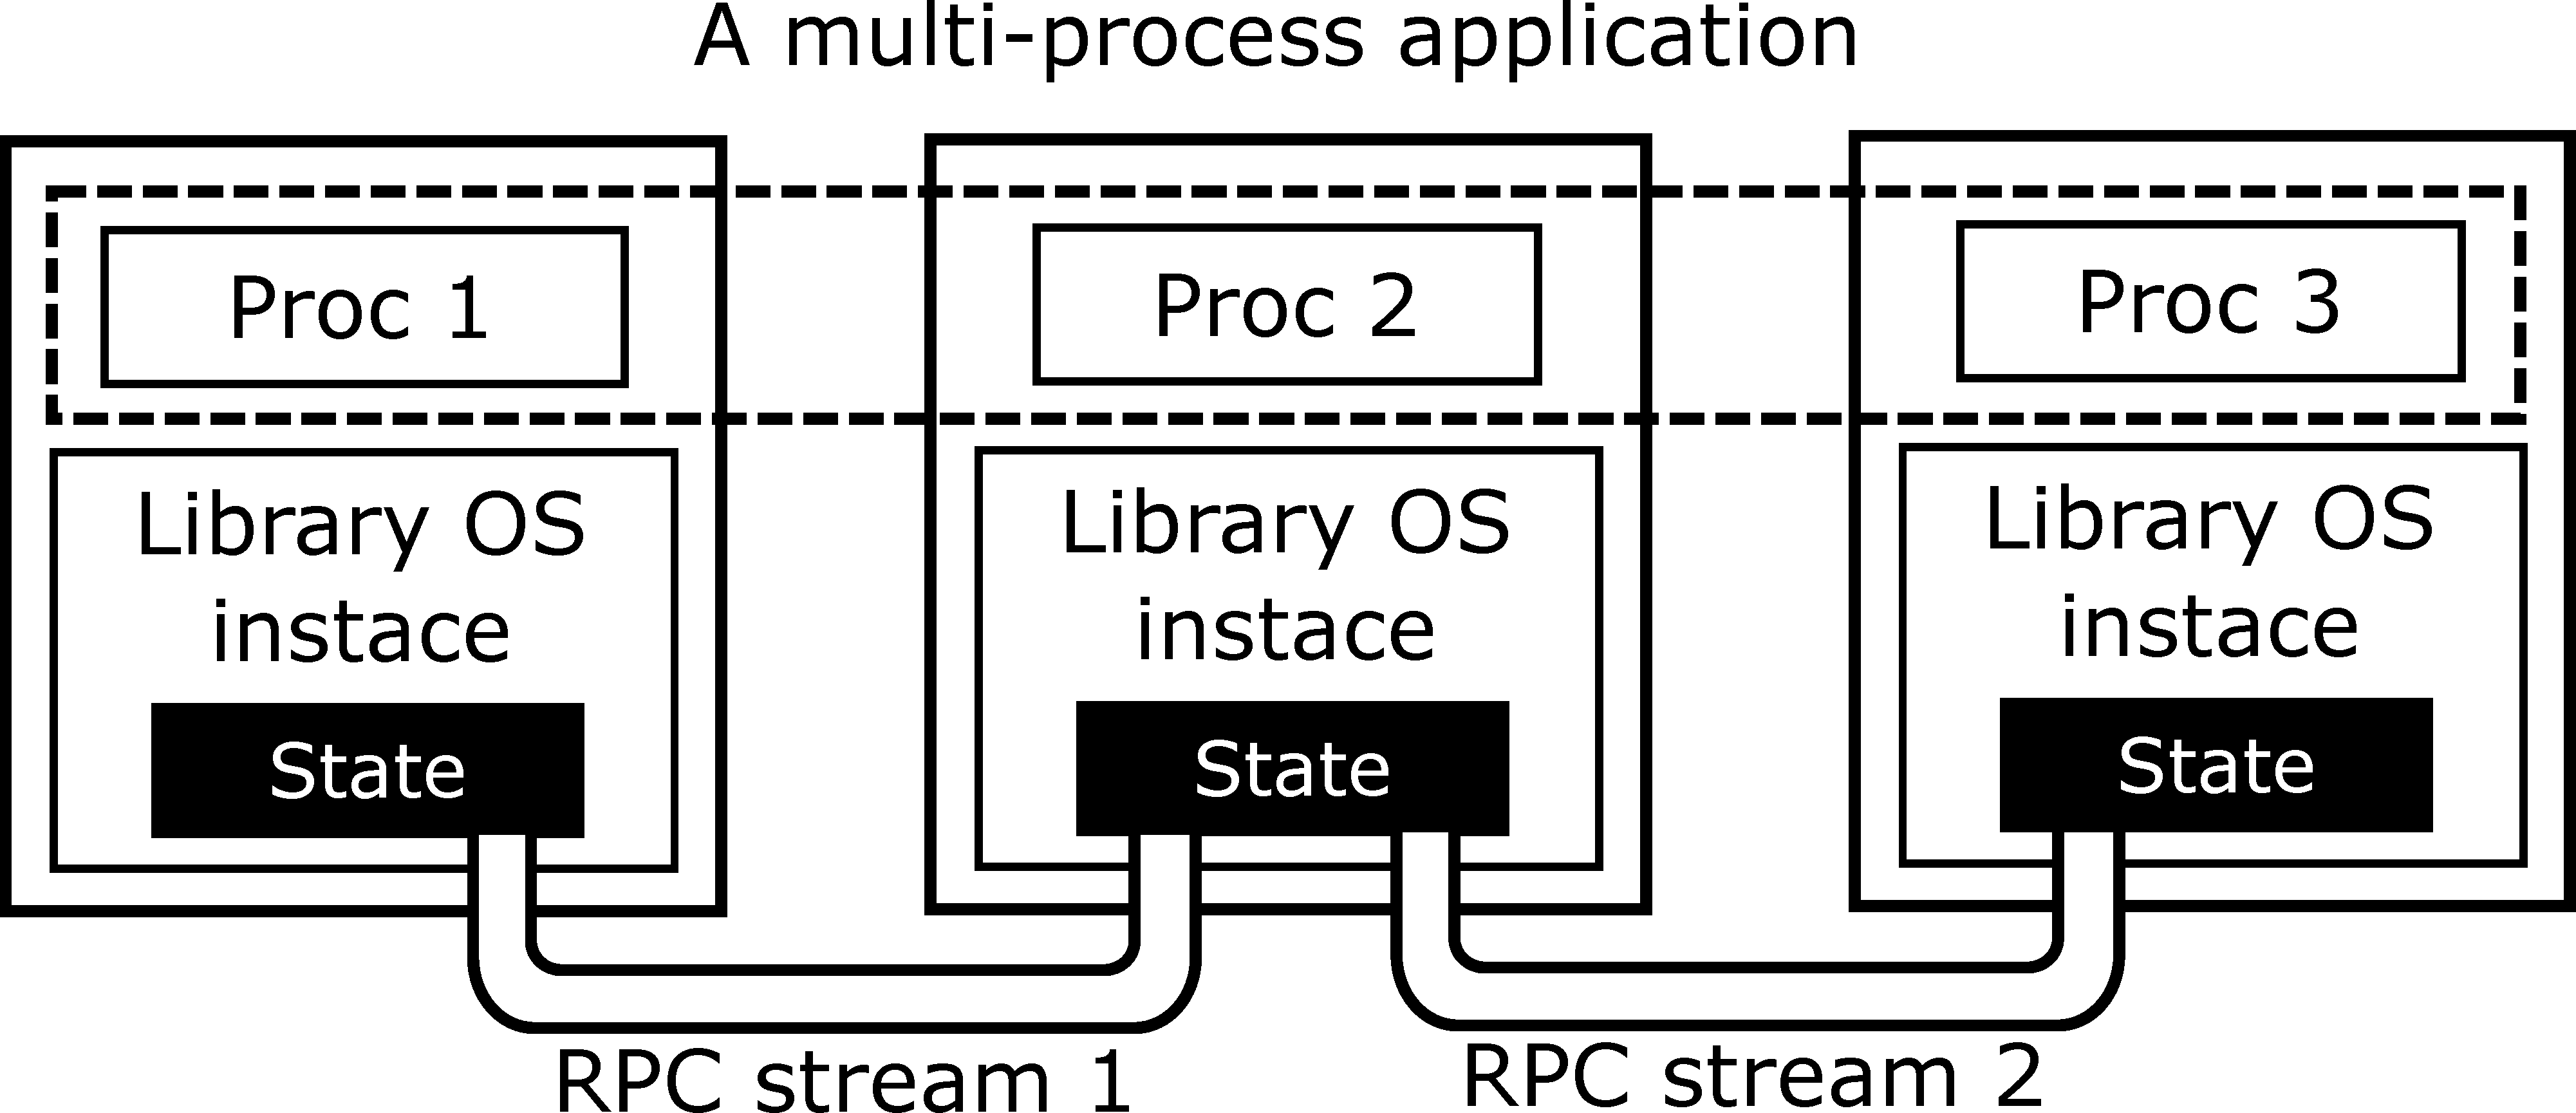
\includegraphics[width=24em]{concept.pdf}
\caption{Multi-process support model of \graphene{} \libos{}. For each process of an application, a \libos{} instance will serve system calls and keep local OS states. States of multi-process abstractions are shared by coordinating over host-provided RPC streams, creating an illusion of running in single OS for the application.}
%\vspace{-.1in}
\label{fig:graphene:concept}
\end{figure}

%{\bf \graphene{}} is a Linux-compatible library OS to run legacy, unmodified Linux applications. 
In \graphene{}, multiple library OS instances collaboratively implement
Linux abstractions, but present single, shared OS view to the application.
\graphene{} instances coordinate states
using message passing over RPC streams.
With a distributed POSIX implementation,
%placement of shared state and messaging complexity are first-order performance concerns.
%%We chose to shift implementation complexity into the library OS
%%in order to uphold simple enforcement of security isolation in the host.
%By coordinating shared states across library OS instances, 
\graphene{} can create an illusion of running in a single OS for multiple processes in an application.

%Previous library OS designs ensured security isolation of independent applications,
%comparable to a VM, by keeping a relatively narrow host ABI.
%We selected the \graphene{}
%design because it strikes a unique balance between
%and robust, flexible security enforcement.
%The \graphene{} design ensures security isolation of
%mutually distrusting, multi-process
%applications on the same host system.
%Essential to this goal is
%minimally expanding the host ABI to support multi-processing,
%as well as leveraging RPCs as a natural point to mediate inter-\picoproc{} communication.
%RPC coordination among \graphene{} instances can be dynamically disconnected, facilitating novel sandboxing
%techniques.  For instance, we develop an Apache web server extension that, upon logging in a given user,
%places the worker process's \libos{} in a sandbox with access to only that user's data.
%We expect more nuanced degrees of trust are possible in future work.

%\graphene{}'s design gives the user and system administrator a high degree of flexibility
%in isolating arbitrary groups of unmodified application processes,
%while upholding the efficiency and host compatibility benefits of recent library OSes.

%\fixmedp{After a complete draft is written, coalesce all goals and make sure they are addressed early on.  We are doing some scatter-shot motivation}


\papersubsection{\Libos{} architecture}
\label{sec:overview:libos:arch}

%Recent library OSes~\cite{porter11drawbridge,unikernels,baumann13bascule,osv}
%are designed for security and efficiency, but are limited to single-process applications.
%The security isolation of \liboses{} derives from 
%limited, explicit data sharing and 
%a narrow host interface.  
A \libos{} typically executes in either a para-virtualized VM~\cite{unikernels,osv}
% \daniela{I would have the use of a VM as a discussion topic in the end of the paper.}, 
or an OS process called a \emph{\picoproc{}}~\cite{porter11drawbridge,baumann13bascule}, with a restricted host ABI.
%The host ABI heavily restrict effects outside of the application's address space
%as a result, applications in a \picoproc{} have very little opportunity to interfere with each other,
%yielding security isolation comparable to a VM.
%The library OS deduplicates features for hardware management in both the guest and host kernels.
\graphene{} executes within a \picoproc{} (Figure~\ref{fig:overview:arch}),
which includes an unmodified application and its supporting libraries, which run alongside a library OS instance.
The \graphene{} \libos{} is implemented over \thehostabi{} designed to expose very generic abstractions that are easy to port on any host OS.
%Although the \graphene{} prototype  host kernel is Linux, 
%we adapt a host ABI from Drawbridge/Bascule,
%which has been previously implemented on \win{}, Hyper-V, and Barrelfish~\cite{porter11drawbridge,baumann13bascule,baumann09barrelfish}.
%The \graphene{} host ABI is
% summarized in Table~\ref{tab:abi} and discussed in more detail in \S\ref{sec:linux:pal}\fixmedp{if not cut...}.  
%which exposes only tens of simple host calls. \daniela{briefly define \picoproc{}: A \picoproc{} is unmodified application code running with a \libos{}.}


\begin{figure}[t]
\centering
\begin{minipage}[b]{1.25in}
\footnotesize
\raggedleft
Linux system calls \\
\graphenesyscallnum{} out of \linuxsyscallnum{}\\
\vspace{0.1in}
Host ABI \\
\palcallnum{} \hostapis{}\\
\vspace{0.2in}
\hostsyscallnum{} Linux system calls
\vspace{0.35in}
\end{minipage}
\hspace{-1.25in}
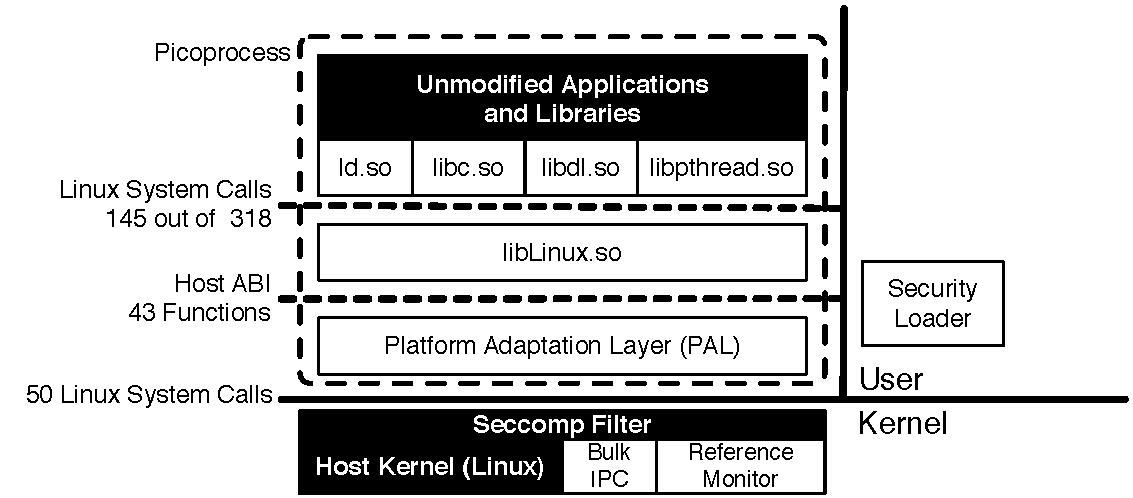
\includegraphics[width=32em]{arch.pdf}
\caption{Building blocks of \graphene{}.  Black components are unmodified.
We modify the four lowest application libraries on Linux:
{\tt ld.so} (the ELF linker and loader),
{\tt libdl.so} (the dynamic library linker),
{\tt libc.so} (standard library C),
and {\tt libpthread.so} (standard threading library), that issue Linux system calls as function calls directly to {\tt libLinux.so}.
Graphene implements the Linux system calls using a variant of the Drawbridge ABI, which is provided by the platform adaption layer (PAL).
A trusted reference monitor that ensures \libos{} isolation is implemented as a kernel module. Another small module is added for fast bulk IPC, but it is optional for hosts other than Linux.}
\label{fig:overview:arch}
\end{figure}


%\graphene{} shows the sufficiency of \thehostabi{} to support a rich Linux \libos{}.
As an example of this layering, consider the heap memory management abstraction. Linux provides applications with a data segment---a legacy abstraction dating back to original UNIX and the era of segmented memory. The primary thread's stack is at one end of the data segment, and the heap is at another.  The heap grows up (extended by \syscall{brk}) while the stack grows down until they meet in the middle.
In contrast, the host ABI provides only minimal abstractions for allocating, deallocating, and protecting regions of virtual memory.
This clean division of labor encapsulates idiosyncratic abstractions
in the library OS.


%These interfaces are host-independent \daniela{OS or kernel-independent}, as they tend to be very generic and easily
%implemented on any host OS kernel or VMM \daniela{postpone VMM for later}.

At a high level, a \libos{}
scoops the layer just below the system call table out of the OS kernel
and refactors the code as an application library.  
The driving insight is that there is a natural, functionally-narrow division point 
one layer below the system call table
in most OS kernels.
Unlike many OS interfaces, \thehostabi{} minimizes the amount of application state in the kernel, facilitating
migration. A \libos{} instance can programmatically read and modify its OS state, copy the state to another instance, and the remote instance can 
load a copy of this state into the OS---analogous to hardware registers.
A \picoproc{} may not modify another \picoprocs{}' OS states.



\papersubsection{Multi-process abstractions}
\label{sec:overview:libos:multiproc}


\issuedone{1.3.b}{An overview of multi-process support}
A key design feature of UNIX is that users compose simple utilities to create more significant applications.  Thus, it is unsurprising that many popular applications are multi-process---an essential feature missing from previous \liboses{}.
%This gap is filled by the \graphene{} \libos{}, which
%extends recent \liboses{} to support multi-process applications.
The underlying design challenge is minimally expanding a tightly-drawn isolation boundary without also exposing idiosyncratic kernel abstractions or re-duplicating mechanisms in both the host kernel and the library OS.

%requires a careful balance among the competing goals of 
%efficiency, host independence, and security isolation.
%The challenge, then, is minimal expansion of

%\vspace{5pt}
%\noindent {\bf Motivating Example.~}
For example, consider the process identifier (PID) namespace. In current, single-process library OSes, \syscall{getpid} could just return a fixed value to each application.
This single-process design is isolated, but the library OS cannot run a shell script, which requires forking and executing multiple binaries, signaling, waiting, and other PID-based abstractions.

%\paragraph{Design options.}
%Multi-process support requires extensions to the host ABI of recent, single-process library OS designs. Because multi-process abstractions, such as signals or System V IPC, tend to be idiosyncratic, an essential problem is identifying a minimal, host-independent substrate upon which  to implement OS-specific abstractions.
There are two primary design options for multi-process abstractions in \liboses{}: (1) implement processes and scheduling in 
the library OS; (2) treat each library OS instance as a process and distribute the shared POSIX implementation across a collection of library OSes.
\graphene{} follows the second option, which imposes fewer host assumptions.
%, maximize flexibility in mapping processes to physical resources, and facilitate inter-process security policy enforcement. % as enforcing security policies on related processes.

Multi-process abstractions
inside the library OS also possibly benefit from
hardware MMU virtualization, similar to
the model explored by Dune~\cite{belay12dune}.
However, this design reintroduces a duplicate scheduler and memory management.
Moreover, Intel and AMD have similar, but mutually incompatible MMU virtualization support,
which would complicate live migration across platforms.
None of these problems are insurmountable, and it would be interesting in future
work to compare both options.


In \graphene{}, multiple \liboses{} in multiple picoprocesses collaborate to implement shared abstractions. \graphene{} supports a rich of Linux multi-process abstractions including copy-on-write forking, \syscall{execve}, signals, exit notification, and System V IPC semaphores and message queues.
For instance, when process A signals process B on \graphene{}, A's library OS instance issues a query to B's instance over a pipe-like
RPC stream, and B's instance then calls the appropriate signal handler.
The host OS is unaware of the implementation
of multi-process abstractions,
as well as security isolation of the corresponding states.

%%% All collaborating \libos{} instances exchange messages as needed 
%%% to provide the application with a consistent view of 
%%% shared abstractions,
%%% such as


%\graphene{} approaches multi-processing by selectively replicating state and issuing remote procedure calls (RPCs) 
%%across multiple, collaborating
%library OS instances.
%Guests may work together to provide the unmodified multi-process application with
%coordination abstractions 

%%Shared abstractions on \graphene{}'s are implemented outside of the host, ensuring  host OS independence.
%% by implementing these
%%shared abstractions entirely
%%outside of the host kernel.
%%Shared abstractions are implemented outside of the host.
%%From the host kernel's perspective, 
%\graphene{} implements all shared abstractions by cooperatively managing the abstraction states over RPC streams.
%Single-process applications still service system calls from local state, and \graphene{}, includes optimizations to place state where it is most likely to be used, minimizing RPC overheads.
%The host reference monitor can easily isolate picoprocesses by 
%% \graphene{} design isolates \liboses{} by 
%%requiring all coordination to use 
%%explicit bytes streams \daniela{, pipe-like abstractions provided by the kernel. (suggestion: Reviewer  3)}.
%%Security isolation is enforced
%%by a kernel-level {\em reference monitor}, which can 
%%disconnect or prevent creation of a
%blocking all RPC messages, % between \liboses{} that should be isolated,
%without the need to understand the library OS details or semantics of these abstractions.
%In the PID example, only mutually-trusting picoprocesses can signal each other.
%%if the reference monitor prevents creation of RPC streams
%%across mutually untrusting \picoprocs{},
%%the \liboses{} cannot exchange signals.

%%% \graphene{} is designed to 
%%% The \graphene{} design leverages a number of optimizations to service application system calls 
%%% from local state whenever possible, and to minimize message passing overheads otherwise
%%%  (\S\ref{sec:namespaces:insights}).
%%% Our experience is that starting with a local system call design and then extending it to share state is relatively straightforward,
%%% and introduces little-to-no overhead when the request can be serviced locally.


The \graphene{} library OS is also capable of gracefully handling disconnection from other library OSes, facilitating dynamic application sandboxing.
RPC streams may disconnect at any time by either the reference monitor or at the request of a library OS.
%Message streams may be severed externally, by the reference monitor, or 
%one guest may simply disconnect from others to isolate itself.
%An application may disconnect itself from the 
%Any \graphene{} application may dynamically detach from the confederation, 
%or a host-level sandbox may dynamically separate two guests by severing their communication channels.
When a picoprocess is disconnected, the library OS will handle the subsequent
divergence, %and the library OS will will fork these abstractions
{\em transparently} to the application.
For instance, if a child process disconnect RPC streams from the parent by the reference monitor, the library OS will interpret the event as if the other process terminated, close any open pipes, and deliver exit notifications.
% \daniela{(applications run unmodified) - Reviewer 1 asked clarification on transparently}.

%% A key insight behind our design is that the common use case for these \daniela{cooperating} abstractions
%% is between a pair of processes.  Thus \graphene{} leverages a number of optimizations 
%% to reduce broadcast messages, avoid replication of needless state,
%% and service requests locally


\paragraph{Comparison with microkernels.}
The building blocks of \graphene{} are very similar to the system abstractions of a 
microkernel~\cite{liedtke95sosp,klein09sel4,elphinstone13microkernels,liedtke93sosp,chen93memory,baron1985mach-1,accetta86mach}, except a microkernel often has an even narrower, more restricted interface than the host ABI.
%such as the port and
%message abstractions of Mach~\cite{
A multi-server microkernel system, such as GNU Hurd~\cite{hurd} or Mach-US~\cite{stevenson95mach-us}, implements Unix abstractions across a set of daemons that are shared by all processes in the system. \graphene{}, on the other hand, implements system abstractions as a library in the application's address space and coordinates library state among \picoprocs{} to implement shared abstractions. \graphene{} guarantees isolation equivalent to running 
an application on a dedicated VM; it is similar to implementing the security isolation model on a multi-server microkernel by running a dedicated set of service daemons for each application.

%%% \graphene{}'s differences are motivated by two considerations: efficient support of both stand-alone, 
%%% single-process applications and multi-process applications; as well as flexible security isolation. 
%%% \graphene{} contributes techniques to seamlessly and efficiently transition 
%%% between single-process and multi-process support, as well as adapting 
%%% some known techniques to a new environment.

%The \graphene{} host ABI could be described as a hybrid microkernel, which also exposes the file system and network of the host kernel.
%Similarly, picoprocesses are assumed to be provided by a production OS, like Linux or \win{}, or by a Type 2 hypervisor.  A bare metal hypervisor could potentially export a PAL, but would require services from a trusted VM, such as Xen's dom0~\cite{barham03xen}.
%%or the \pal{} would implement more thread scheduling, networking, and file system code;
%%or the \pal{} ABI would change to push this code into the \libos{}.
%Arguably, recent library OS designs might be improved by rethinking the division of labor, but this is beyond the scope of this thesis.

%\paragraph{Alternatives.}
%Another approach to support multi-process applications in a library OS would be to use hardware MMU virtualization such as nested paging used by a system like Dune~\cite{belay12dune}
%in order to implement a second process abstraction, memory manager, and scheduler in the library OS.
%This approach threatens the efficiency benefits of deduplicating these features.
%A final option is exposing additional system interfaces, such as signals, by adding more system calls to a picoprocess. This approach undermines compatibility, as many of these coordination abstractions tend to be very OS-specific.
%%Unix signals vs.\ \win{} events, {\tt waitpid()} vs.\ blocking on a process handle, etc.
%%Although legacy OSes do enforce some access control rules on coordination abstractions,
%%kernel developers must audit and add hooks to millions of lines of code.
%%As a result,
%%users have lost confidence that a traditional OS can comprehensively enforce 
%%security isolation on these abstractions---a key motivation for using VMs
%%for security isolation.


%Systems must strike a careful balance between the competing goals of
%security isolation and multi-process coordination.
%Multi-process applications require OS-managed coordination abstractions such as signals, process exit notification, and System V IPC.
%These coordination abstractions operate within shared namespaces, such as the process ID namespace and the System V key space.
%These coordination APIs and namespaces must be consistent among coordinating processes, but can undermine security isolation among unrelated processes on the same host.
%System designs generally only meet one goal: traditional OSes have a rich but porous coordination interface, while sandboxing systems and VMs are strictly isolated.
%This thesis demonstrates that this unfortunate trade-off is not fundamental.
%coordination or isolation.  


%Traditional OS kernels typically provide  rich multi-process coordination APIs, but this richness also makes for a very porous attack surface area.  For instance, on \win{}, a program may inject libraries and create threads in another program~\cite{windows-dll-inject}; 
%similarly, unchecked file descriptor inheritance in Linux can lead to security problems~\cite{close-on-exec}.  
%Although legacy OSes do enforce some access control rules on these abstractions, kernel developers must audit and add hooks to so much code that users have lost confidence that an OS can comprehensively enforce security isolation on these abstractions.

%For achieving strong security isolation on applications, users have turned to VMs.
%For instance, if two customers host their websites in the same cloud service, the customers will insist on running their web servers in separate VMs for security.
%VMs take a heavy-handed approach to security isolation---ensuring that every application has a dedicated OS kernel in a hardware-isolated address space.
%Although virtual machines isolate applications and provide legacy OS abstractions within a VM, coordinating applications must be statically placed in the same VM,
%and cannot dynamically move to a separate VM.
%For instance, consider a web service running inside of a VM that wishes to isolate requests for different users in different VMs after authentication.  The web server administrator must statically create a VM for each user, introducing substantial
%overhead; and the developer loses convenient IPC abstractions and must rewrite large swaths of code.

\section{Summary}
\label{sec:graphene:summary}

The \graphene{} design is centered around
building a para-virtualized layer, which can reuse the OS components for reproducing Linux system interfaces.
%instead of building arbitrary compatibility layers for reproducing the system interface.
%constantly porting the significant  of the existing system interface.
%In \graphene{}, 
\graphene{} defines a host ABI, as a new boundary between the OS and user space.
The host ABI is simple enough to port (containing \palcalls{} functions),
and exports sufficient functionality for virtualizing a primary part of the system API components.
A library OS is built upon the host ABI,
and implements \graphenesyscalls{} Linux system calls to reuse unmodified Linux applications.
\graphene{} decouples the development for a compatibility layer,
from host-specific challenges to building OS features, and isolating applications from other malicious tenants.



%\sysname{} extends library OS designs 
%to include multi-process APIs required by common applications, such as a shell or 
%web server.
%\sysname{} demonstrates efficient, selective
%coordination of shared state across multiple library OS 
%instances---maintaining host independence.
%%simplifying security sandboxing of otherwise unwieldy OS features.
%Applications on \sysname{} enjoy both 
%strong security isolation with acceptable performance and low memory overheads.
%% from unrelated programs 
%%and seamless shared namespaces 
%%among a group of coordinating guests.
%%% Although this paper focuses on distributed coordination
%%% to facilitate the efficiency benefits,
%%% expect our experiences with distributed coordination 
%%% may also be particularly relevant to highly scalable OS designs, 
%%% which avoid the bottlenecks of shared OS data structures~\cite{baumann09barrelfish, song11eurosys}.
%%Graphene's overheads are acceptable and the memory 
%%footprint is substantially lower than a VM.



%% , which could benefit from the reduced memory footprint
%% in a cloud 

%% by introducing a novel design for  coordination APIs. 
%% to a new OS (Linux),
%% new classes of applications,
%% and introduces a
%% %an alternative design point for storage virtualization.
%% Our results further demonstrate the feasibility of the library OS model.
%% % generally,
%% Applications on Graphene enjoy both 
%% strong security isolation from unrelated programs 
%% and seamless shared namespaces 
%% among a group of coordinating guests.
%% Although we explore this concept in a library OS,
%% we expect the namespace coordination framework 
%% could also be adapted to limit the attack surface area between
%% processes in a traditional OS.
%% We expect these experiences with distributed coordination 
%% may also be particularly relevant to highly scalable OS designs, 
%% which avoid the bottlenecks of shared OS data structures~\cite{baumann09barrelfish}.
%and specifically of content-addressable storage as the primary virtual storage abstraction.
%%% This work opens up a number of interesting questions for future work, 
%%% including studying opportunities for low-level storage optimization within the CAS server,
%%% making CAS the root file system,
%%% eliminating storage management in the host kernel, and 
%%% investigating the impact of frequent migration among devices.

\begin{comment}
Enabling legacy applications in a restricted environment,
such as \picoprocs{} or enclaves,
requires extra effort for mitigating the limitations of platforms,
in order to support typical OS personalities.
\graphene{}, as described in this chapter, extends the existing \libos{} designs
from isolating single-process or unshared abstractions
to include multi-process APIs required by many UNIX applications,
such as servers or shell scripts.
The challenge that \graphene{} primarily overcomes
is the requirement for coordinating shared states across multiple \picoprocs{},
to provides a collaborative, unified OS view.
Essentially, \graphene{} implements all shared, multi-process abstractions
and OS states
based on coordination over host-provided, pipe-like RPC streams.
The RPC-based, distributed OS implementation enables multi-process support in \graphene{}, with minimal extension to the host interface,
and a sweet-spot for enforcing inter-application security isolation,
by simply sandboxing the RPC streams.
Such a model largely reduces the complexity of
enforcing security isolation
on idiosyncratic multi-process abstractions
and shared states.
Because the corporative nature of \picoprocs{} in \graphene{},
an application can even dynamically impose sandboxing on one of its processes,
to reflect per-process, variable security policies.
\end{comment}

\begin{comment}
In principle, we attempt to use \graphene{} to justify the platform independence
of the \libos{} design,
without sacrificing its qualitative benefits,
such as isolating mutually-untrusting applications
and a narrow attack surface to kernels.
\graphene{} implements a considerable number of common Linux system calls,
to support popular, modern applications
such as Apache web server, GNU Make, OpenJDK \java{} VM and the Python runtime.
\graphene{} translates the high-level system APIs used by applications
to a host ABI
inherited and extended from a previous Windows-compatible \libos{}~\cite{porter11drawbridge}.
In addition, we port the \pal{} (Platform Adaption Layer) of \graphene{}
to various platforms,
including FreeBSD, OSX, Windows, and even a more restricted environment, the \intel{} \sgx{} enclaves.
In particular, \graphene{} being ported to \intel{} \sgx{}
(\graphenesgx{})
can isolate applications --- either single-process or multi-process
--- on a host where neither the operating system nor the hardware (except the CPU package)
is trusted by the applications. 
Overall, \graphene{} shows that,
by simply porting the reasonably sized host ABI
to a new platform,
a whole large spectrum of legacy applications tested on the previous platforms
can be activated all together.
\end{comment}

\makeatletter
\def\input@path{{}}
\makeatother
\graphicspath{{}}
%%% dp: This title is pretty vague.  
%\section{Addressing the Combination of \java{} and \sgx{}}
\section{\java{} Support for Partitioning into \sgx{}}
\label{sec:civet:concept}

This section explains the support \sysname{} adds to \java{}
for partitioning applications into \sgx{} enclaves.
%support in addresses the challenges
%in partitioning \java{} applications on 

\subsection{Cleanly partitioning classes and objects}
\label{sec:civet:concept:partition}

%To address the partition challenge in a managed language like \java{},
%\sysname{} diminishes the need for developers
%to scrutinize the whole code base
%and identify the fine line of isolating trusted and untrusted classes. 

\sysname{} includes Shredder to automatically partition \java{} applications on \sgx{},
requiring  minimal developer effort.
Figure~\ref{fig:civet:builder} shows the workflow of a developer using the \sysname{} Shredder tool.
The developer selects the application's main class, either as a JAR or class files
and the classpath of the library.
The developer also specifies the list of
entry classes that should be in the enclave and export an interface to the code 
outside of the enclave.
%% When developers use the tool to partition their applications, they provide
%% the application package, either in JAR or classes,
%% the class paths of the depended libraries,
%% and a list of {\em entry classes} as the initial entry points of the enclave.
The Shredder then
identifies all classes that the entry classes depend upon,
until the transitive closure of these dependencies converges.
%performs {\bf dependency tracking} starting at the entry classes,
%until all the depended classes eventually converge.
%% dp: this feels out of place here; maybe put it at the beginning of the section?
%Afterward, \sysname{} packages the classes, with additional steps of augmentation, instrumentation, and signing, purpose of which is explain in \S\ref{sec:concept:loading} and \ref{sec:concept:accessing}.

\begin{figure}[t!]
\centering
\includegraphics[width=4.5in]{civet/figures/building-tool.pdf}
\caption[\sysname{}: overview of the design-time tool.]
{The \sysname{} design-time tool, for partitioning, packaging, augmentation, instrumentation, and signing.
\sysname{} partitions the \java{} application based on the entry classes
specified by the developers (classes {\tt Trusted}).
The Shredder tool recursively pulls all required supporting classes into the 
package to run in the enclave.
%from all the class paths.
%Only the minimum necessary classes are kept for the enclave,
The Shredder tool creates an enclave JAR file after augmentation,
instrumentation, and signing.}
\label{fig:civet:builder}
\end{figure}

The Shredder creates a single package with all dependencies of the
entry classes.
This is a reasonable simplification, although 
% for two reasons.  First, 
%loading all required classes from a single package is 
%is a reasonable simplification 
%that matches expected practice for enclaves.
%We note that 
it would be relatively easy in future work to add more signed JAR-style packages,
if needed.
This approach also allows us to 
reduce the attack surface and overheads by minimizing the 
enclave entry and exit points, albeit at the expense of duplicating some supporting
classes in and out of the enclave.
%\fixmedp{sounds like we don't let enclave code call out to classes? Might bear some discussion whether this is a limitation or not}

%% We argue that partition based on entry classes and
%% dependency tracking at class granularity
%% is sufficient for isolating the trusted and untrusted components.
%% There are basically two goals for our partition tool:

%% \begin{compactenum}
%% \item To create a static package of supporting classes, so \sysname{} runtime can load every required class from the package.
%% \item To avoid the isolated execution from leaving the enclave,
%% in between the entry triggered by method invocation
%% from the untrusted components,
%% and returning the control to the untrusted components.
%% \end{compactenum}


Unless the application explicitly asks the class loader to
dynamically load a class,
every piece of code needed during the execution of trusted classes
is included in the enclave image.
The image includes classes that are used in dynamic casting and parent classes 
that contain code inherited by the trusted classes.
Shredder also includes any required supporting JNI libraries in the image.
Shredder does not attempt to partition the JNI libraries to a smaller binary,
which we leave for future work.

%Because \java{} maintains type-safety in most cases \fixmedp{is it not always type safe?},
%any classes that have ever been cast to in the application can be tracked as a dependency. Methods that are inherited from the parent classes
%are also covered in dependency tracking.

%If an application will ever request for dynamic loading using class names,
%the developers must specify the classes in the partition tool.
%The case that dynamic loading is needed is most commonly seen in the crypto APIs:
%for example, to instantiate a {\tt Cipher} object,
%the applications will provide a string that describes the transformation
%of the cipher, such as {\tt AES/CBC/PKCS5PADDING}.
%Based on the string, the method {\tt Cipher.getInstance()} will load classes
%{\tt AESCipher}, {\tt PCBC}, and {\tt PKCS5Padding}.
%The rationale behind dynamic loading is that no matter
%which class name the application request for,
%the class loader will only search among the trusted classes,
%so no malicious classes will be loaded.

%% \sysname{} also includes any JNI 
%% In the case that any supporting classes require JNI,
%% \sysname{} will include the correspondent JNI libraries in the enclave image.
%% The JNI libraries are unpacked when the enclave starts,
%% and added to {\tt LD\_LIBRARY\_PATH} for the trusted \java{} VM.
%% \sysname{} currently does not partition the JNI libraries, but we see the partition of JNI as a manageable future work. 

Based on our case studies (\S\ref{sec:civet:cases}),
we observe that specifying the entry classes and identifying any dynamically loaded classes,
requires minimal developer effort.
In all of our use cases, the applications are partitioned with only one entry class, and very few dynamically loaded classes.


%\sysname{} transparently handles all the details of accessing \sgx{} hardware,
%in behave of the loaded \java{} applications (as shown in figure~\ref{fig:synthesis}).
%When \sysname{} is called to run isolated \java{} components,
%it creates two worlds of \java{} execution --- one is in the enclave and the other is outside the enclave.
%With the ability of running \java{} classes inside the enclave,
%\sysname{} can support the partitioned model with both isolated and untrusted classes implemented as \java{} classes.

%\begin{table*}[t!b!]
\centering
  \begin{tabular}{p{0.05in} >{\raggedright\arraybackslash}p{2.05in} >{\raggedright\arraybackslash}p{4.4in}}
  \toprule
  \multicolumn{2}{l}{\it Security guarantees or features} & {\it The modeling approach applied by \sysname{}} \\
  \midrule
  \midrule
  \multicolumn{3}{l}{\bf Natively provided by the \sgx{} hardware (including the SDK):} \\
  \midrule
  & Isolating security-sensitive components &
  Asking developers to identify multi-level sensitivity, by marking the {\em entry classes}. Complete separation between isolated and untrusted classes.
  \\
  \midrule
  & Secure entry / exit of enclaves &
  Exporting public methods of isolated classes. Arguments are type-checked.
  \\
  \midrule
  & Integrity of the execution environment & 
  Packaging all supporting classes into a signed JAR.
  \\
  \midrule
  & Attestation \& secure provisioning & 
  Providing class {\tt Enclave}, to create secure channels and exchange attestation.
  \\
  \midrule
  \midrule
  \multicolumn{3}{l}{\bf Improvement from combining of \java{} language and the \sgx{} hardware protection:} \\
  \midrule
  & Memory safety \& control flow integrity &
  Naturally provided by \java{} language.
  \\
  \midrule
  & Reducing the enclave TCB &
  Automated partitioning based on class dependencies.
  \\
  \midrule
  & Preventing information flow leakage &
  Tracking information flow in trusted classes, only allow releasing the information if not tainted or declassified by developers.
  \\
  \midrule
  & Code confidentiality & Dynamically loading provisioned classes.
  \\
  \end{tabular}
  
\footnotesize
\caption{
The approaches applied by \sysname{} to model the security guarantees and features of the \sgx{} hardware, and to enhance the security by combining language and hardware protections.
}
\label{tab:features}
\end{table*}


%Even though \sysname{} hides the low-level semantics of the \sgx{} hardware from the applications,
%the applications still have full access to the security guarantees ({\em what is secured?}) and features ({\em how is it secured?}) provided by the the \sgx{} hardware.
%We do so by identifying the high-level goals of these guarantees and features,
%and remodel the goals in the \java{} language.
%The underlying mechanisms of these goals is the original guarantees and features provided by the \sgx{} hardware.

%We discuss each security guarantee or features of the \sgx{} hardware,
%and how they are actually modeled in \sysname{} as follows.

%\paragraph{Isolated execution of security-sensitive components}
%The \sgx{} hardware ensures components with higher security sensitivity
%to be executed inside the enclave
%and completely isolated from the components that are less security sensitive.
%The isolated components shall not share any data with the untrusted components unless the isolated components decide
%to flow the data out of the enclave.  

%\sysname{} models this guarantee by asking the developers to make
%the classes that they believe to be security sensitive.
%Note that only the top-most classes that interact with the untrusted components have to be identified --- we can these classes as the {\em entry classes}.
%After developers identifying the multi-level security sensitive with an application, \sysname{} uses a building tool to partition the application
%based on the developers' hint.
%The partition completely separates the \java{} classes for the isolated components from the classes for the untrusted components.
%The execution of these isolated classes will be fully jailed inside the enclave, and any invocation of the methods exported by the isolated classes
%from the untrusted classes
%will be re-routed into the enclave.
%The returned values of the invoked methods will be routed back to
%the untrusted classes,
%either as proxies of the actually returned instances (if the instances are not yet safe to release from the enclave) or the actual values.



\subsection{Dynamically loading byte-code with integrity}
\label{sec:civet:concept:loading}


After the Shredder partitions the applications
and creates an enclave image as a JAR file,
developers can ship the enclave image with the rest of the application.
The application is then executed on an untrusted host with the 
%to the untrusted hosts that have the 
\sysname{} runtime framework installed.
%Then, on the untrusted hosts users will run the application,
Upon the first use, either by creating a trusted object or calling a static method of a trusted class,
%Whenever an entry class is instantiated, or one of its static method is invoked,
the \sysname{} runtime framework creates an enclave containing the trusted classes.

%\fixmedp{Trusted and isolated are used pretty interchangeably.  Pick one keyword and use it consistently, please}

Figure~\ref{fig:civet:runtime} shows the structure of the \sysname{} runtime framework(a more detailed view of Figure~\ref{fig:civet:synthesis}).
The \sysname{} runtime framework is split into the front-end (untrusted) and the back-end (trusted).
When the front-end calls into a trusted class,
it finds enclave image that contains the class,
checks if an enclave is created for the same image in the current \java{} VM,
and, if not, creates an enclave.
The trusted classes from the same image share an enclave.
%and \sysname{} does not support the scenarios that the developers want to 
%further partition the trusted classes.

\sysname{} runs a separate, lighter-weight \java{} VM in the enclave.
Running a \java{} VM in the enclave is a subtle challenge because a \java{} VM
often yields a large system API footprint, and, by default, uses a large heap. % requires access to abundant resources such as the heap.
To provide the required OS APIs inside the enclave, we use the Graphene library OS~\citep{tsai14graphene}~\footnote{Downloaded from \url{github.com/oscarlab/graphene}}.
In order to remove unneeded features and balance resource utilization with performance in current SGX enclaves, such as
a 128 MB limit on the size of the enclave page cache,
we adjust the build-time configuration of the JVM to change multithreaded garbage collector to single threaded, remove multiple JIT engines and stop non-essential threads in the JVM. 

%Moreover, a production \java{} VM like \jvm{} is implemented in
%millions of lines of code \fixme{get the actual number},
%which will cost tremendous effort to port into \sgx{} enclaves.

%To avoid the cost of porting the \java{} VM, \sysname{} uses {\em Graphene-SGX library OS}~\citep{graphene-sgx} 
%to facilitate the OS features needed by the \java{} VM.
%Therefore, we do not modify any code of \jvm{}, except tuning the compilation options to reduce its resource usage.

%\fixme{I am gonna avoid saying Graphene from now on.}
When \sysname{} creates an enclave, the \sgx{} hardware measures integrity of the initially-loaded library OS.
The library OS then loads \jvm{} and all of the supporting libraries,
such as {\tt libc},
the JLI (\java{} legacy interface) library, and the minimal \java{} classes needed to bootstrap the class loader.
Finally, \java{} VM loads the enclave image JAR file.

Graphene itself is responsible to maintain the code integrity of the JVM.
%\sysname{} depends on Graphene-SGX to maintain the code integrity.
When Graphene loads a binary or class files,
it verifies the integrity of the files by checking their measurements.
The measurements of binary or class files are also
hashed into the enclave measurement,
so no attacks can bypass the integrity check or manipulate Graphene to load  a malicious \java{} VM or bogus enclave image.

If an application requests dynamic loading by a class name,
the developers must specify the classes to the Shredder tool.
The case that dynamic loading is needed is most commonly seen in the crypto APIs:
for example, to instantiate a {\tt Cipher} object,
the applications provide a string that describes the transformation
of the cipher, such as {\tt AES/CBC/PKCS5PADDING}.
Based on the string, the method {\tt Cipher.getInstance()} loads classes
{\tt AESCipher}, {\tt PCBC}, and {\tt PKCS5Padding}.
The rationale behind this restriction on dynamic loading is that, no matter
which class name the application requests,
the class loader only searches among the trusted classes,
so no malicious classes will be loaded.
\fixmedp{Seems like you could also do a signature check at runtime, and there are other ways to relax this requirement, but whatever.}

%\paragraph{Integrity of the execution environment}
%The \sgx{} hardware must guarantee the execution of the isolated components
%is exactly the same as developed, tested and verified by the application developers.
%The \sgx{} hardware verify the cryptographic measurement of loaded binaries
%at the creation of the enclave,
%and can generate attestation that the enclave is created with such measurement.
%The purpose of the guarantee is to prevent code injection,
%unless the isolated applications are tricked into loading the code by the attackers.

%\sysname{} models this guarantee by creating a snapshot of developers'
%execution environment, including the version of \java{} VM,
%checksums of any infrastructure binaries,
%and the minimal supporting classes for the isolated component. 
%\sysname{} packs all these files into a JAR file and sign it with the developers' private key.
%When \sysname{} creates an enclave, the hardware measurement of the enclave includes only the infrastructure, as the \java{} VM and the \sysname{} back-end.
%Once the enclave is created, the \sysname{} back-end must  
%check whether the JAR file loaded has the correct signature.

\begin{figure}[t!]
\centering
\includegraphics[width=4.5in]{civet/figures/civet-structure.pdf}
\caption[\sysname{}: framework overview.]
{\sysname{} framework overview.
\sysname{} creates two worlds for an partitioned \java{} application, each with an individual JVM.
The JVM in the enclave is ported using Graphene library OS.
Untrusted classes can invoke methods of trusted classes through proxy objects,
which can transparently access the enclave interface, through serialization
and deserialization over an ring buffer accessed by both untrusted JVM and trusted JVM. }
\label{fig:civet:runtime}
\end{figure}


\subsection{Seamless access to in-enclave objects}
\label{sec:civet:concept:interface}

For programmer convenience, 
untrusted code can seamlessly call in-enclave objects in \sysname{}.
This is particularly useful when application components are closed-source.
All public methods of trusted, programmer-identified entry classes are entry points for the enclave.
The \sysname{} runtime framework is responsible for generating glue code for entering and exiting
the enclave appropriately, tracking references to objects in the enclave, 
as well as marshalling arguments and return values for in-enclave functions.

%in \sysname{},
%access to in-enclave objects seamless for the untrusted components.
%The rationale behind this design is based on two reasons.
%First, the target of method invocation in \java{} is identified dynamically
%via referencing the object.
%Second, \sysname{} intends to avoid the developers' effort for injecting explicit entry points into the untrusted components,
%especially when the imported \java{} class libraries are close-source.

%% As \sysname{} dynamically determines the enclave entry points in the untrusted components,
%% it avoids the requirement for developers
%% to define the untrusted interface of the enclave.
%% Instead of inquiring manual definition,
%% \sysname{} applies a simple principle to automatically determine the entry points:
%% All public methods of the {\em public} trusted classes can be entry points of the enclave.

In order to reference objects inside the enclave from outside the enclave,
\sysname{} framework uses a byte code generation library --- {\em CGLib}~\citep{cglib} to create untrusted proxies for the in-enclave instances.
CGLib instruments the class that is being proxied,
and redirects the control to a handler 
assigned by \sysname{} upon any method invocation on the proxy.
The proxy then triggers enclave entry to run the trusted method.



%% When untrusted code calls a public method of a trusted class,
%% \sysname{} transparently identifies 
%% determines enclave entry based on whether the objects accessed is in the enclave or part of the untrusted components.
%% As classes can be replicated inside and outside the enclave,
%% the same method of the same class must trigger different behavior according to the sensitivity of the instances.
%% If the object is instantiated in the untrusted components, the method must be run outside the enclave.
%% If the object is instantiated in the enclave, the method should be trapped,
%% and trigger enclave entry to run the method.
 
In general, supporting classes can be duplicated inside and outside of the enclave.
Calls to a supporting class, such as {\tt String}, from inside of an enclave
go to the in-enclave version, and calls from outside the enclave go to the untrusted version.

An exception is made for entry classes, which are not allowed to be replicated.
Rather, any call to an entry class function is placed inside the enclave.
Thus, constructors and static methods of entry classes also cause enclave entries.
We note that this design point was taken to minimize programmer effort in porting to SGX;
alternatively, we could allow an entry class to be replicated by requiring the programmer to 
explicitly annotate calls to object functions.

The \sysname{} design-time tool creates untrusted proxy classes for all entry classes,
in which all constructors and static methods are redirected to
the \sysname{} front-end, which then enters the enclave.
We chose this approach because CGLib disallows redirecting 
constructors and static methods, as this can introduce ambiguity in
the invocation target when all classes are in the same JVM.

%% If the method called is a constructor or static method,
%% the affected object is no longer an instance,
%% but the class itself.
%% To allow seamless invocation of the method,
%% it causes ambiguity for the affiliation of the class, if the class is replicated in both partitions.
%% Therefore, \sysname{} restricts the invocation of constructors or static methods
%% to only the entry classes,
%% and disallows replicating the entry classes
%% in the untrusted components.
%% In addition, if the constructor of an entry class is called upon the constructor of its untrusted subclass,
%% the instantiation will be rejected by \sysname{}.

%% \paragraph{Interception of in-enclave objects.}
%% To seamlessly trigger the enclave entry upon method invocation,
%% \sysname{} intercepts the instances or classes that belong to the isolated components.
%% To intercept non-static method of in-enclave instances,
%% \sysname{} uses {\em CGLib} \fixme{cite} to create proxies of the in-enclave instances.
%% CGLib instruments the class that is being proxied,
%% and redirect the control to a handler assigned by \sysname{} upon any method invocation on the proxy.
%% The handler then triggers enclave entry to run the isolated method.

%% \sysname{} uses a different mechanism of interception for constructors and static methods,
%% because CGLib disallows redirecting constructors and static method
%% due to the ambiguity of invocation targets.
%% Instead, \sysname{} uses the design-time tool to create a dummy classes for all the entry classes,
%% in which all constructors and static methods are redirected to
%% the \sysname{} front-end.
%% Because we disallow replication of entry classes
%% in the untrusted components,
%% loading the dummy classes does not affect functionalities of the application. 

\paragraph{Passing arguments into the enclave.}
When a method triggers enclave entry, the arguments of the method have to be passed into the enclave for the invocation.
\sysname{} always copy the arguments into the enclave,
by serializing the arguments into byte streams,
copying the byte streams into the enclave memory,
and then de-serializing into objects.
By coping arguments into the enclave,
\sysname{} ensures execution of trusted code does not inadvertently leave the enclave.
If the code invokes a method on one of the arguments,
the in-enclave copy of the class is used on an in-enclave instantiation of the object.
Upon de-serialization, the arguments are also automatically type-checked,
thus avoiding the risk of memory corruption.

\paragraph{Returning objects.}
Once the triggered method finishes execution in the enclave,
it may return an object or literal back to the untrusted calling function.
In general, objects are returned similarly to passing input arguments---by serializing the object to a byte stream and returning the bytes.
%Technically, returning objects is the same as passing arguments, and only take serialization and de-serialization.

In order to ensure confidentiality of sensitive data, \sysname{} takes additional care to check
whether a returned object creates an unexpected control flow.
At enclave exit, \sysname{} only allows an object to be returned if it is not tainted with any secret data,
in which case the object is serialized and passed back to the caller.
Section~\ref{sec:civet:security} details our information flow tracking mechanism.

In cases where the object is tainted and an instance of a trusted class,
\sysname{} instead creates a reference in the enclave (to prevent garbage collection of the object internally),
and returns an opaque reference type, that causes the untrusted \sysname{} runtime to create a proxy out of the enclave.
This policy applies to all constructors.
If a proxy object is garbage collected, the destructor calls into the enclave to release the reference on the 
corresponding object in the enclave.
The \sysname{} untrusted runtime is responsible for translating any proxy objects passed as arguments to the enclave into opaque pointers,
which the in-enclave runtime then translates to local object references.

In the case of a tainted literal, we encrypt the plaintext return value concatenated with a nonce, using a temporary key, and return the ciphertext.
This encrypted literal can then be passed to subsequent enclave calls, where the value is decrypted as part of deserialization.

%% However, unconditionally allowing returning objects may become a threat to the information confidentiality of the enclave,
%% because the object may contain part of the enclave secrets due to the information flow.
%% \sysname{} only allows returning objects
%% that are not tainted by the information flow from any secrets. More details about determining the taintedness of the objects are discussed in section~\ref{sec:civet:security}.

%% Based on the taintedness of the objects, \sysname{} has different policies and mechanisms of returning the objects to the caller,
%% to maintain both information confidentiality and progress of the application.
%% The policies are described as follows:

%% \begin{compactitem}
%% \item {\bf the object is not tainted}: serialize and pass the object to the caller.
%% \item {\bf the object is tainted, and is instance of an isolated class}: 
%% create a proxy and intercept future invocation.
%% The policy commonly applies to all constructors.
%% \item {\bf the object is tainted, and is a literal}:
%% automatically encrypt the literal with a default key.
%% \end{compactitem}


%\paragraph{Secure entry and exit of the enclave}
%The \sgx{} hardware ensures that the enclave only has fixed number of entry points (exactly one location where the execution starts, but multiple pre-defined locations that the execution can jump to). 
%The untrusted components must be forbidden to jump to random code in the enclave.
%Moreover, if the isolated component want to exit the enclave,
%it must explicit call the exit instruction ({\tt EEXIT}) to make sure
%the control flow won't be manipulated to leave the enclave.

%\sysname{} models this guarantees by exporting all the public methods of the isolated classes
%(including constructors, static and non-static methods) as the entry points or untrusted interfaces.
%When the untrusted component calls a constructor or static method of an isolated class,
%the execution inside the enclave is triggered,
%either to instantiate the class or perform other operations.
%If a proxy of an isolated instance is returned to the untrusted components,
%the untrusted components can keep it or pass it around.
%As soon as any untrusted components call one of the public methods on the proxy, the execution re-enter the enclave and start the isolated execution.

%Exporting public methods as the entry points or the untrusted interface
%is assumed to be reasonably secure in \sysname{}.
%First, only for the entry classes (the top-most classes of the enclave),
%the constructors or static method will be exported.
%Because developers have expressed that these classes are the ones that interact with the untrusted classes, it is safe to allow the untrusted components to calls these methods and trigger execution in the enclave.
%Second, even if the public non-static methods can be called
%upon isolated classes, the untrusted components can only call upon the proxies,
%which are essentially returned values from the previous method calls.
%Without the proxy, the untrusted components can never call the public methods
%on random instances in the enclave, if the instances are never returned to the untrusted components.


\subsection{Remote Attestation and Provisioning}
\label{sec:civet:concept:others}

\paragraph{Generating attestation reports.}
A feature of \sgx{} hardware is the ability to generate an attestation report for a remote entity,
demonstrating the integrity of the enclave code at launch time.
%The \sgx{} hardware provides the feature of generating a attestation report to prove the integrity of the isolated execution to a remote entity.
\sysname{} provides helper API for developers to access these features,
with convenience and extended trust.
For attestation, \sysname{} generates a report that contains a list of classes loaded inside the enclave, with their measurements.
The report is attached with the attestation generated and signed by \sgx{}, but processed by Graphene.
The \sgx{}-generated attestation contains both
the enclave measurement (proving integrity of Graphene) and
the measurement verified by Graphene (proving integrity of other binaries and files).


%% \fixmedp{Huh?  Really?}
%% The attestation report contains the enclave measurement
%% and is signed using a key derived
%% from the measurements of both sides of attesters,
%% so the remote entity can verify it by retrieving the same key
%% (both attesters must be running in \sgx{} enclaves).

Note that \sysname{} also includes
the dynamic loading state in the attestation report.
%A stronger guarantee provided by \sysname{} than \sgx{}
%is to present the dynamic loading state in the attestation report.
The attestation generated by \sgx{} only contains
the initial state of the enclave, and does not record changes within the executable code
after the enclave starts. 
In both cases, the remote entity is trusting the initially loaded binary
to not dynamically load code that could compromise the enclave;
however, \sysname{} can offer a more precise accounting of the state of the enclave 
at the time a report is generated.

\fixmedp{For future work, would be cool to have some non-editable record of what is added to the enclave, so a corrupted enclave cannot hide the equivalent of a rootkit}

%% As a result, the entity that
%% verifies the attestation report has to blindly trust the initial code
%% in the enclave does not dynamically load any vulnerable code.  
%% The attestation report generated by \sysname{}
%% reflects the latest state of class loading,
%% allowing the trusted entity to audit the execution of enclaves.

% providing a class called {\tt Enclave}, with the APIs that service attestation and provisioning requests.
%The {\tt Enclave} APIs are wrapper to the low-level semantics required by the \sgx{} hardware,such as exchanging the attestations with remote hosts and verifying them, or 
%securing the channels after attesting the other side of communication.
%Because the works are completely hidden beneath the APIs,
%the developers are spared from all the cryptographic details during the process of attestation and provisioning.

\paragraph{Secure provisioning.}
\sysname{} provides an API that transparently validates a connection to a remote host to load
sensitive classes or secret data.
%to be used for secure provisioning.
To use this API, both sides of the connection
must be running in enclaves created by \sysname{}.
The API performs key exchange algorithm (e.g., Diffie-Hellman) on the connection,
secure the connection with encryption,
and authenticate the connection by exchanging the attestation reports.
\sysname{} provides convenient helper functions for developers to create a trusted path
for provisioning sensitive data to a remote enclave.
%Developers can use this API to design any provisioning scheme, without implementing the details of building the trusted path.


\section{Hardening \sgx{} at Enclave Boundary using Information Flow Control in \java{} }
\label{sec:civet:security}

\sysname{} % models the high-level security guarantees and features
%of the \sgx{} hardware in the \java{} language,
allows \java{} developers to directly utilize the security features of \sgx{}, such as isolation from an untrusted hypervisor, % execution, code integrity, etc,
in combination with language-level features that make the code in the enclave more robust.
% safety and advanced protections in \java{}.
%By bridging the gap between language and hardware protections,
%\sysname{} creates opportunities to combine \sgx{} hardware protections
%and security benefits given by \java{} as a managed language.
%In this section, we discussed the opportunities we explore to harden \sgx{} protection with the usage of \java{} language.

%\fixmedp{Honestly, a lot of this is getting pretty repetitive.  I would probably hoist the argument for Java into the motivational text and not bother repeating it here.}

%\subsection{Benefits from the usage of \java{} Language}

%We note that \java{} has several features that can reduce or eliminate
%common vulnerabilities.
%Memory corruption bugs are constant threats to applications
%implemented in C or C++ languages,
%but \java{} applications naturally defend against these vulnerabilities.
%\java{} is immune from memory corruption bugs, such as heap and buffer overflows.
%Several security enhancements come naturally with running \java{} classes
%in the enclave. \java{} applications are known to be immune to memory corruption bugs such as buffer or heap overflow.
%Type casting in \java{} is checked against the type of the target object.
%applications, \java{} perform strict type-checking on the objects to be casted.
%Type-checking prevents corruption of object either in the isolated components,
%or when receiving arguments from the untrusted interfaces.
%Similarly, 
%Similar as the memory corruption bugs,
%Because \java{} is memory safe, it is immune to known control flow attacks, such as return-oriented programming,
%where control flow is manipulated by unsafe writes to return pointers on the stack or function pointers in objects.
%applications implemented in C or C++ languages inevitably face the risk of ROP (return-oriented programming) attacks,
%where attackers can manipulate the control flow by corrupting the applications' stacks or heaps.
%Since \java{} classes can defend against memory corruption,
%attacks cannot manipulate the control flow by overriding the return pointers or function pointers.

%We do assume that the JVM and JNI code are free from memory corruption and control flow attacks.
%Proving a JVM implementation correct is beyond the scope, although similar 
%efforts have been made previously to prove a language runtime correct~\citep{yang10safe}.
%In the case of JNI, we would discourage developers from using JNI code in enclaves if at all possible.

%% Note that although memory corruption bugs and control flows attacks are forbidden in \java{} classes,
%% these vulnerabilities can still exist in the \java{} VM and JNI.
%% In \sysname{} we assume \java{} VM and JNI must be fully trusted,
%% and we leave it as a future work to secure these components.

%% dp: Meh.  prolix
%% For isolated components in the enclaves, memory corruption bugs and control flow attacks are just as dangerous as for other applications.
%% Because the isolated components are fully trusted by the CPU,
%% they can access any memory that are set to proper permissions, including the memory outside the enclaves.
%% Even if a vulnerable component is exploited to copy all the enclave secret out of the enclaves, no hardware solution can effectively stop the exploitation.
%% Even though isolated components cannot directly jump out of the enclave,
%% control flow attack can still manipulate the components to jump to certain locations internally and perform malicious operations. 
%% Therefore, preventing memory corruption bugs and control flow attacks
%% can be a strong reason for application developers
%% to choose \java{} language instead of C/C++ to implement the isolated components.

%\fixmedp{This whole subsection is already covered above.  Commenting}
\begin{comment}
\subsection{Reducing the enclave TCB}

%A \java{} applications often yield a huge TCB, including the \java{} VM,
%JNI and supporting classes that come in bulk.
%For example, a \java{} applications executed by \jvm{}
%will load the \java{} VM binaries up to 40MB \fixme{find out actual numbers}. The classes in the standard \java{} VM libraries such as {\tt rt.jar} includes more than 18,000 classes, and the size of the package is more than 30MB.
%On the other hand, the actual classes needed by an application from {\tt rt.jar}
%can be as less as 1,000 classes.
%Majority of the classes provided from {\tt rt.jar},
%--- even though they may never be loaded into the enclave ---
%still remains in the TCB.

Having unnecessary binaries and classes in the TCB of the enclave
can aggravate the risk of being attacks.
First of all, the huge amount of code loaded into the enclave
increase the opportunity of having gadgets that can be exploited in ROP attacks,  
which can still happen in the \java{} VM or JNI.
Even though most of the \java{} classes have static footprint of their supporting classes,
many of them still dynamically load classes, such as directly calling the class loader, or specifying providers to the \java{} cryptography framework.
Having huge TCB as \java{} classes in the enclave still intensify
the risk of attacks, even though \java{} classes are immune to control flow attacks. 

\sysname{} largely reduce the supporting classes that can be loaded into the enclave,
by partitioning out the necessary classes from all the libraries in the developers' class paths, into the enclave image.
When the enclave is created, the \java{} VM will not load any existing libraries such as {\tt rt.jar} from the host system,
but instead only search classes in the signed enclave image.
Minimizing the supporting classes that can be loaded into the enclave
guarantees that all the classes that are included in the TCB
are actually required by the isolated components,
and come from a trusted source such as the developers' execution environment. 

Note that we do not partition the JNI within the \java{} VM binaries.
We assume partitioning out the JNI functions that are required by the isolated classes
is fully feasible with some manageable efforts.
Moreover, the \java{} classes can be potentially partitioned at a smaller granularity than the whole classes, such as the methods and fields, which can even further reduce the TCB.
We leave these potential improvements as future works. 
\end{comment}

%\subsection{Information Flow Control at Enclave Boundary}
%Problem of not just leaking secrets but also tainted info
As an example of higher-level, language-based analysis, we implemented information flow tracking
in \sysname{}.
A common usage of enclaves is to protect sensitive data, such as an encryption key;
thus, a common concern is that this sensitive data not be inadvertently returned because of an error or exploit within the enclave code.
In general, we chose a design point that minimizes programmer effort; to adopt information flow tracking, we
do require the programmer to specify secret data classes and declassify objects to be released as is from the enclave.

\begin{figure}[t!]
\centering
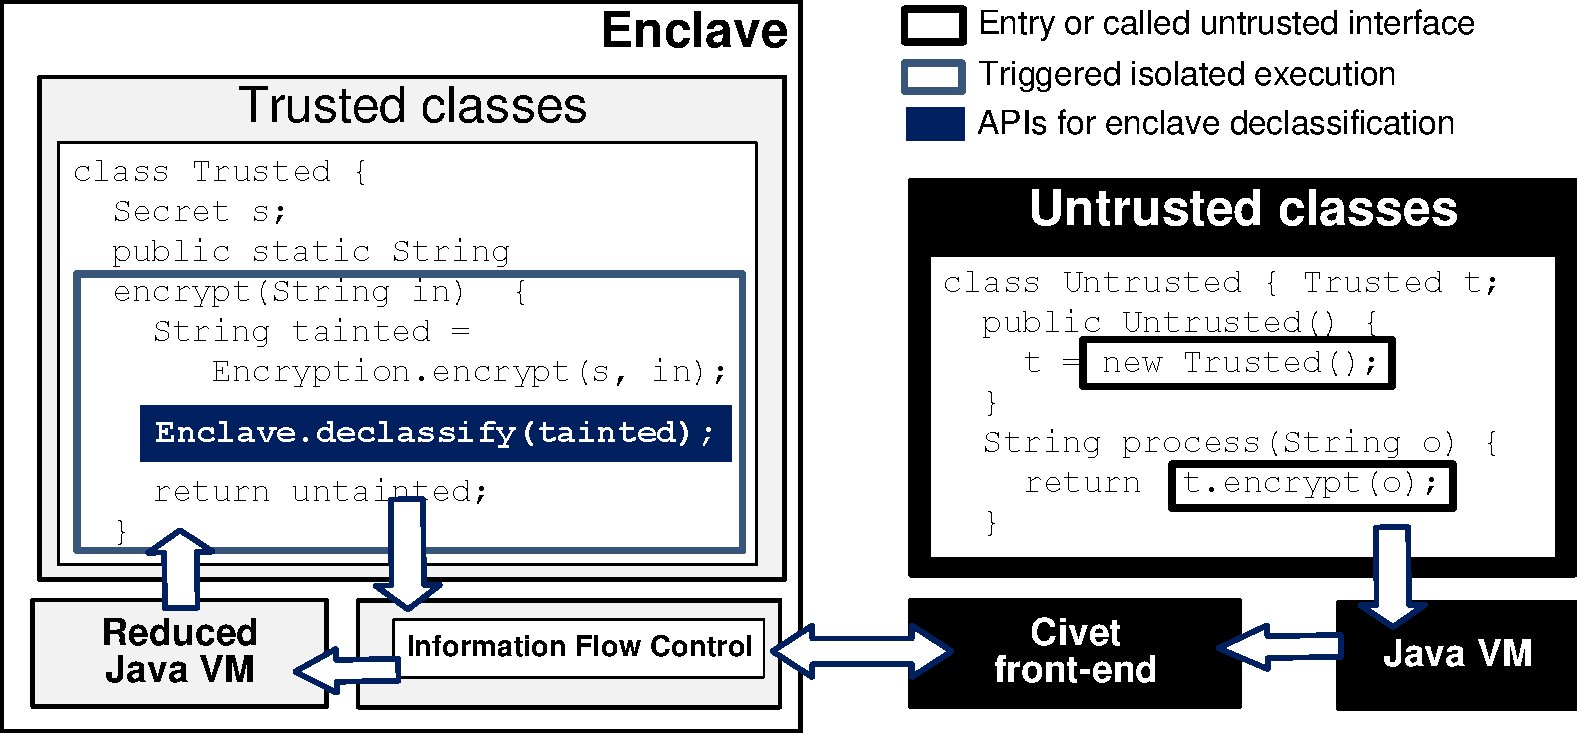
\includegraphics[width=3.2in]{civet/figures/declassify.pdf}
\footnotesize
\caption[\sysname{}: declassifier APIs.]
{How \sysname{} provides declassifier APIs to declassify sensitive data.
When the untrusted class ({\tt Untrusted}) from Figure ~\ref{fig:civet:synthesis} now calls the {\tt encrypt} method of a trusted class ({\tt Trusted}),
\sysname{} automatically calls the {\tt encrypt} method inside enclave, and pass the {\tt String} parameter.
Before returning the result, the trusted class has to use the {\tt declassify} to remove the taint of {\tt tainted} variable that is tainted by the {\tt encrypt} method of class {\tt Encryptor} because of the tainted secret variable {\tt s}.
}
\label{fig:civet:declassify}
\end{figure}

%Because the code running in enclave has access to complete address space, including the trusted as well as untrusted memory regions, it is easy for the trusted code to inadvertently undermine \sgx{} protection by writing secret information in the untrusted region. Further, leaking any information derived from or related to the secret may be used by the untrusted code to guess the value of secret information. For example, even in the presence of memory protection, sandboxing and virtualization, it is possible to recover the secret key used by crypto algorithms~\citep{kocher1996timing,osvik2006cache,weiss2012cache, zhang2012cross}. So, to ascertain the secrecy of the sensitive data, no information derived from the secret should exit enclave in plaintext.

%We use JAVA tool phosphor source and sink to taint provisioned data and control leakage
%\sysname{} leverages extensive research on information flow tracking and control in \java{} to harden the \sgx{} security. 

In the enclave, we implement source-to-sink taint tracking, using the open-source Phosphor library~\citep{phosphor}.
%\fixmedp{check this}
The programmer manually selects the classes containing secret data that take secret input from a remotely-provisioned source.
This taint is propagated to any new variables that result from explicit or implicit flows from a secret object.
The only way to remove taint from an object is to pass the object through a \sysname{} declassifier API,
which returns an untainted copy of the object.

%\fixmedp{Would be nice to have a simple example class with a label and declassifier in a figure, if space and time allow}

\sysname{} enforces the policy that only untained data may be returned from an enclave.
If tainted data is being returned, the system transparently encrypts the data and removes its taint before letting the data leave the enclave.
In the cases where a developer wants to return references to sensitive data, \sysname{} instead returns an opaque reference or, in the case of a literal, encrypts the return value.

%mFor tainted data, the developer may opt to either throw a runtime error, or, by default, to return an encrypted object instead.
%The en

% to taint the secret data when provisioned and propagate the taint to any new data generated as an explicit or implicit result of the secret data. We specify the enclave exit points as targets and enforce the policy that any tainted data must pass through a declassifier, that encrypts the data before egress. We only consider the provisioned data as security sensitive, as the enclave image is only integrity protected.

%Declassifier API: correct usage and scenarios
The \sysname{} {\tt Enclave} class provides a {\tt declassify(Object o)} API that creates an untainted
copy of the object.  In practice, we expect this function to be used in conjunction with tests
on the returned data, or cryptographic functions to protect the data in transit across an untrusted channel.

Continuing our example from Figure~\ref{fig:civet:synthesis}, in Figure~\ref{fig:civet:declassify}, if the {\tt Untrusted} class wants to call the {\tt encrypt} method on the trusted object {\tt t}, \sysname{} front-end transparently passes the argument string {\tt o} to the enclave, and the corresponding {\tt encrypt} method is called in the enclave. The secret {\tt s} is tainted because it was provisioned from remote trusted server as shown in Figure ~\ref{fig:civet:synthesis}. As a result, the call to method {\tt encrypt} of class {\tt Encryptor} taints the encrypted output string {\tt tainted}. If the developer had returned this {\tt tainted} variable, the \sysname{} information flow tracking would re-encrypt the ciphertext, and thus make the return value useless for the {\tt Untrusted} class. However, as the developer wants to return the ciphertext as is, she can declassify the {\tt tainted} string by passing it through the declassifier API to get an untainted version of the same object. Such untainted objects can be released from the enclave without further encryption.

%to let the application developer explicitly indicate that the argument object does not contain any secret information, and is safe to leave the enclave as is. For instance, if the enclave code encrypts a blob of data using the tainted secret provisioned key, the information flow will taint the encrypted data. However, because the encrypted data is safe to exit enclave if a perfectly secure encryption algorithm is used, the developer can explicitly mark the encrypted data as declassified. We note that the developers need to be extra careful while declassifying objects to inadvertently leaking secret information.

%Dealing with confidential code
In order to protect the confidentiality of sensitive code,
\sysname{} also allows classes themselves to be tainted.
\sysname{} enforces a policy that any data returned from sensitive code is tainted, and the developer needs to explicitly declassify tainted output data to mitigate
concerns around reverse-engineering the code based on brute-force probing of its outputs.
Of course, the binary code itself is also not allowed to be copied out of the enclave.

% expose it to the untrusted world.
%The {\em code confidentiality} property of \sysname{} loads and executes encrypted classes from remote hosts to protect secret algorithm. We consider this provisioned code as equally security sensitive as provisioned data. ~

%\begin{table*}[t!b!]
\centering
  \begin{tabular}{p{0.05in} >{\raggedright\arraybackslash}p{2.05in} >{\raggedright\arraybackslash}p{4.4in}}
  \toprule
  \multicolumn{2}{l}{\it Security guarantees or features} & {\it The modeling approach applied by \sysname{}} \\
  \midrule
  \midrule
  \multicolumn{3}{l}{\bf Natively provided by the \sgx{} hardware (including the SDK):} \\
  \midrule
  & Isolating security-sensitive components &
  Asking developers to identify multi-level sensitivity, by marking the {\em entry classes}. Complete separation between isolated and untrusted classes.
  \\
  \midrule
  & Secure entry / exit of enclaves &
  Exporting public methods of isolated classes. Arguments are type-checked.
  \\
  \midrule
  & Integrity of the execution environment & 
  Packaging all supporting classes into a signed JAR.
  \\
  \midrule
  & Attestation \& secure provisioning & 
  Providing class {\tt Enclave}, to create secure channels and exchange attestation.
  \\
  \midrule
  \midrule
  \multicolumn{3}{l}{\bf Improvement from combining of \java{} language and the \sgx{} hardware protection:} \\
  \midrule
  & Memory safety \& control flow integrity &
  Naturally provided by \java{} language.
  \\
  \midrule
  & Reducing the enclave TCB &
  Automated partitioning based on class dependencies.
  \\
  \midrule
  & Preventing information flow leakage &
  Tracking information flow in trusted classes, only allow releasing the information if not tainted or declassified by developers.
  \\
  \midrule
  & Code confidentiality & Dynamically loading provisioned classes.
  \\
  \end{tabular}
  
\footnotesize
\caption{
The approaches applied by \sysname{} to model the security guarantees and features of the \sgx{} hardware, and to enhance the security by combining language and hardware protections.
}
\label{tab:features}
\end{table*}


%% dp: This title is pretty vague.  
%\section{Addressing the Combination of \java{} and \sgx{}}
\section{\java{} Support for Partitioning into \sgx{}}
\label{sec:concept}

%\fixmets{1.5 page}

This section explains the support \sysname{} adds to \java{}
for partitioning applications into \sgx{} enclaves.
%support in addresses the challenges
%in partitioning \java{} applications on 

\subsection{Cleanly partitioning classes and objects}
\label{sec:concept:partition}

%To address the partition challenge in a managed language like \java{},
%\sysname{} diminishes the need for developers
%to scrutinize the whole code base
%and identify the fine line of isolating trusted and untrusted classes. 

\sysname{} includes Shredder to 
 partition \java{} code for \sgx{},
reducing developer effort.
Figure~\ref{fig:builder} shows the workflow of a developer using the \sysname{} Shredder tool.
The developer selects the application's main class, either as a JAR or class files
and the classpath of the library.
The developer also specifies the list of
entry classes that should be in the enclave and exports an interface to the code 
outside of the enclave.
%% When developers use the tool to partition their applications, they provide
%% the application package, either in JAR or classes,
%% the class paths of the depended libraries,
%% and a list of {\em entry classes} as the initial entry points of the enclave.
The Shredder then
identifies all classes that the entry classes depend upon,
until the transitive closure of these dependencies converges.
%performs {\bf dependency tracking} starting at the entry classes,
%until all the depended classes eventually converge.
%% dp: this feels out of place here; maybe put it at the beginning of the section?
%Afterward, \sysname{} packages the classes, with additional steps of augmentation, instrumentation, and signing, purpose of which is explain in \S\ref{sec:concept:loading} and \ref{sec:concept:accessing}.

\begin{figure}[t!]
\centering
\includegraphics[width=1.0\linewidth]{building-tool.pdf}
\caption{\sysname{} \staticphase{} tool, for partitioning, packaging, augmentation, instrumentation, and signing.
\sysname{} partitions the \java{} application based on the entry classes
specified by the developers (classes {\tt Trusted}).
The Shredder tool recursively pulls all required supporting classes into the 
package to run in the enclave.
%from all the class paths.
%Only the minimum necessary classes are kept for the enclave,
The Shredder tool creates an enclave JAR file after augmentation,
instrumentation, and signing.}
\label{fig:builder}
\end{figure}

The Shredder creates a single package with all dependencies of the
entry classes.
This is a reasonable simplification, although 
% for two reasons.  First, 
%loading all required classes from a single package is 
%is a reasonable simplification 
%that matches expected practice for enclaves.
%We note that 
it would be relatively easy in future work to add multiple, signed JAR-style packages,
if needed.
This approach also allows us to 
reduce the attack surface and overheads by minimizing the 
enclave entry and exit points, albeit at the expense of duplicating some supporting
classes in and out of the enclave.
%\fixmedp{sounds like we don't let enclave code call out to classes? Might bear some discussion whether this is a limitation or not}

%% We argue that partition based on entry classes and
%% dependency tracking at class granularity
%% is sufficient for isolating the trusted and untrusted components.
%% There are basically two goals for our partition tool:

%% \begin{compactenum}
%% \item To create a static package of supporting classes, so the \sysname{} \dynamicphase{} framework can load every required class from the package.
%% \item To avoid the isolated execution from leaving the enclave,
%% in between the entry triggered by method invocation
%% from the untrusted components,
%% and returning the control to the untrusted components.
%% \end{compactenum}


Unless the application explicitly asks the class loader to
dynamically load a class,
every piece of code needed during the execution of trusted classes
is included in the enclave image.
The image includes classes that are used in dynamic casting and parent classes 
that contain code inherited by the trusted classes.
Shredder also includes any required supporting JNI libraries in the image.
Shredder does not attempt to partition the JNI libraries to a smaller binary,
which we leave for future work.

%Because \java{} maintains type-safety in most cases \fixmedp{is it not always type safe?},
%any classes that have ever been cast to in the application can be tracked as a dependency. Methods that are inherited from the parent classes
%are also covered in dependency tracking.

%If an application will ever request for dynamic loading using class names,
%the developers must specify the classes in the partition tool.
%The case that dynamic loading is needed is most commonly seen in the crypto APIs:
%for example, to instantiate a {\tt Cipher} object,
%the applications will provide a string that describes the transformation
%of the cipher, such as {\tt AES/CBC/PKCS5PADDING}.
%Based on the string, the method {\tt Cipher.getInstance()} will load classes
%{\tt AESCipher}, {\tt PCBC}, and {\tt PKCS5Padding}.
%The rationale behind dynamic loading is that no matter
%which class name the application request for,
%the class loader will only search among the trusted classes,
%so no malicious classes will be loaded.

%% \sysname{} also includes any JNI 
%% In the case that any supporting classes require JNI,
%% \sysname{} will include the correspondent JNI libraries in the enclave image.
%% The JNI libraries are unpacked when the enclave starts,
%% and added to {\tt LD\_LIBRARY\_PATH} for the trusted \jvm{}.
%% \sysname{} currently does not partition the JNI libraries, but we see the partition of JNI as a manageable future work. 

Based on our case studies (\S\ref{sec:case-study}),
we observe that specifying the entry classes and identifying any dynamically loaded classes,
is relatively simple.  %requires low developer effort.
In all of our use cases, the applications are partitioned with only one entry class, and very few dynamically loaded classes.


%\sysname{} transparently handles all the details of accessing \sgx{} hardware,
%in behave of the loaded \java{} applications (as shown in figure~\ref{fig:synthesis}).
%When \sysname{} is called to run isolated \java{} components,
%it creates two worlds of \java{} execution --- one is in the enclave and the other is outside the enclave.
%With the ability of running \java{} classes inside the enclave,
%\sysname{} can support the partitioned model with both isolated and untrusted classes implemented as \java{} classes.

%\begin{table*}[t!b!]
\centering
  \begin{tabular}{p{0.05in} >{\raggedright\arraybackslash}p{2.05in} >{\raggedright\arraybackslash}p{4.4in}}
  \toprule
  \multicolumn{2}{l}{\it Security guarantees or features} & {\it The modeling approach applied by \sysname{}} \\
  \midrule
  \midrule
  \multicolumn{3}{l}{\bf Natively provided by the \sgx{} hardware (including the SDK):} \\
  \midrule
  & Isolating security-sensitive components &
  Asking developers to identify multi-level sensitivity, by marking the {\em entry classes}. Complete separation between isolated and untrusted classes.
  \\
  \midrule
  & Secure entry / exit of enclaves &
  Exporting public methods of isolated classes. Arguments are type-checked.
  \\
  \midrule
  & Integrity of the execution environment & 
  Packaging all supporting classes into a signed JAR.
  \\
  \midrule
  & Attestation \& secure provisioning & 
  Providing class {\tt Enclave}, to create secure channels and exchange attestation.
  \\
  \midrule
  \midrule
  \multicolumn{3}{l}{\bf Improvement from combining of \java{} language and the \sgx{} hardware protection:} \\
  \midrule
  & Memory safety \& control flow integrity &
  Naturally provided by \java{} language.
  \\
  \midrule
  & Reducing the enclave TCB &
  Automated partitioning based on class dependencies.
  \\
  \midrule
  & Preventing information flow leakage &
  Tracking information flow in trusted classes, only allow releasing the information if not tainted or declassified by developers.
  \\
  \midrule
  & Code confidentiality & Dynamically loading provisioned classes.
  \\
  \end{tabular}
  
\footnotesize
\caption{
The approaches applied by \sysname{} to model the security guarantees and features of the \sgx{} hardware, and to enhance the security by combining language and hardware protections.
}
\label{tab:features}
\end{table*}


%Even though \sysname{} hides the low-level semantics of the \sgx{} hardware from the applications,
%the applications still have full access to the security guarantees ({\em what is secured?}) and features ({\em how is it secured?}) provided by the the \sgx{} hardware.
%We do so by identifying the high-level goals of these guarantees and features,
%and remodel the goals in the \java{} language.
%The underlying mechanisms of these goals is the original guarantees and features provided by the \sgx{} hardware.

%We discuss each security guarantee or features of the \sgx{} hardware,
%and how they are actually modeled in \sysname{} as follows.

%\paragraph{Isolated execution of security-sensitive components}
%The \sgx{} hardware ensures components with higher security sensitivity
%to be executed inside the enclave
%and completely isolated from the components that are less security sensitive.
%The isolated components shall not share any data with the untrusted components unless the isolated components decide
%to flow the data out of the enclave.  

%\sysname{} models this guarantee by asking the developers to make
%the classes that they believe to be security sensitive.
%Note that only the top-most classes that interact with the untrusted components have to be identified --- we can these classes as the {\em entry classes}.
%After developers identifying the multi-level security sensitive with an application, \sysname{} uses a building tool to partition the application
%based on the developers' hint.
%The partition completely separates the \java{} classes for the isolated components from the classes for the untrusted components.
%The execution of these isolated classes will be fully jailed inside the enclave, and any invocation of the methods exported by the isolated classes
%from the untrusted classes
%will be re-routed into the enclave.
%The returned values of the invoked methods will be routed back to
%the untrusted classes,
%either as proxies of the actually returned instances (if the instances are not yet safe to release from the enclave) or the actual values.



\subsection{Dynamically loading byte-code with integrity}
\label{sec:concept:loading}

A key motivation for dynamic loading is the ability to load encrypted
classes from a remote, trusted host. 
For instance, one may want to load proprietary code into an enclave
that must first be decrypted and then validated, in order to 
protect an implementation of a trade secret.

Shredder creates a partition image as a JAR file, which
developers can ship with the rest of the application.
The application is then executed on an untrusted host with the 
%to the untrusted hosts that have the 
\sysname{} \dynamicphase{} framework installed.
%Then, on the untrusted hosts users will run the application,
Upon the first use, either by creating a trusted object or calling a static method of a trusted class,
%Whenever an entry class is instantiated, or one of its static method is invoked,
the \sysname{} \dynamicphase{} framework creates an enclave containing the trusted classes.

%\fixmedp{Trusted and isolated are used pretty interchangeably.  Pick one keyword and use it consistently, please}

Figure~\ref{fig:runtime} shows the structure of the \sysname{} \dynamicphase{} framework (a more detailed view of Figure~\ref{fig:synthesis}).
The \sysname{} runtime framework is split into the front-end (untrusted) and the back-end (trusted).
When the front-end calls into a trusted class,
it finds enclave image that contains the class,
checks if an enclave is created for the same image in the current \jvm{},
and, if not, creates an enclave.
The trusted classes from the same image share an enclave.
%and \sysname{} does not support the scenarios that the developers want to 
%further partition the trusted classes.

\sysname{} runs a separate, lighter-weight \jvm{} in the enclave.
Running a \jvm{} in the enclave is a subtle challenge because a \jvm{}
often yields a large system API footprint, and, by default, uses a large heap. % requires access to abundant resources such as the heap.
To provide the required OS APIs inside the enclave, we use the \graphene{} \libos{}~\cite{tsai14graphene}~\footnote{Downloaded from \url{github.com/oscarlab/graphene}}.
In order to remove unneeded features and balance resource utilization with performance in current \sgx{} enclaves, such as
a 128 MB limit on the size of the enclave page cache,
we adjust the build-time configuration of the \jvm{} to change multi-threaded garbage collector to single threaded, remove multiple JIT engines and stop non-essential threads in the \jvm{}. 
\fixmedp{say how, more specifically (in English.  You don't need to list specific options, but give us a bit more here}

%Moreover, a production \jvm{} like \jvmname{} is implemented in
%millions of lines of code \fixmets{get the actual number},
%which will cost tremendous effort to port into \sgx{} enclaves.

%To avoid the cost of porting the \jvm{}, \sysname{} uses {\em \sgx{}-\sgx{} \sgx{}}~\cite{graphene-sgx} 
%to facilitate the OS features needed by the \jvm{}.
%Therefore, we do not modify any code of \jvmname{}, except tuning the compilation options to reduce its resource usage.

%\fixmets{I am gonna avoid saying \sgx{} from now on.}
When \sysname{} creates an enclave, the \sgx{} hardware measures integrity of the initially-loaded \libos{}.
The \libos{} then loads \jvmname{} and all of the supporting libraries,
such as {\tt libc},
the JLI (\java{} legacy interface) library, and the minimal \java{} classes needed to bootstrap the class loader.
Finally, \jvm{} loads the enclave image JAR file.

The \graphene{} \libos{} maintains the code integrity of the \jvm{}.
When \graphene{} loads a binary or class files,
it verifies the integrity of the files by checking their measurements.
The measurements of binary or class files are also
hashed into the enclave measurement,
so no attacks can bypass the integrity check or manipulate \graphene{} to load  a malicious \jvm{} or bogus enclave image.

If an application requests dynamic loading by a class name,
the developers must specify the classes to the Shredder tool.
The case where dynamic loading is needed is most commonly seen in the crypto APIs:
for example, to instantiate a {\tt Cipher} object,
the applications provide a string that describes the transformation
of the cipher, such as {\tt AES/CBC/PKCS5PADDING}.
Based on the string, the method {\tt Cipher.getInstance()} loads classes
{\tt AESCipher}, {\tt PCBC}, and {\tt PKCS5Padding}.
The rationale behind this restriction on dynamic loading is that, no matter
which class name the application requests,
the class loader only searches among the trusted classes,
so no malicious classes will be loaded.
\fixmedp{Seems like you could also do a signature check at \dynamicphase{}, and there are other ways to relax this requirement, but whatever.}

%\paragraph{Integrity of the execution environment}
%The \sgx{} hardware must guarantee the execution of the isolated components
%is exactly the same as developed, tested and verified by the application developers.
%The \sgx{} hardware verify the cryptographic measurement of loaded binaries
%at the creation of the enclave,
%and can generate attestation that the enclave is created with such measurement.
%The purpose of the guarantee is to prevent code injection,
%unless the isolated applications are tricked into loading the code by the attackers.

%\sysname{} models this guarantee by creating a snapshot of developers'
%execution environment, including the version of \jvm{},
%checksums of any infrastructure binaries,
%and the minimal supporting classes for the isolated component. 
%\sysname{} packs all these files into a JAR file and sign it with the developers' private key.
%When \sysname{} creates an enclave, the hardware measurement of the enclave includes only the infrastructure, as the \jvm{} and the \sysname{} back-end.
%Once the enclave is created, the \sysname{} back-end must  
%check whether the JAR file loaded has the correct signature.

\begin{figure}[t!]
\centering
\includegraphics[width=1.0\linewidth]{civet-structure.pdf}
\caption{\sysname{} framework overview.
\sysname{} creates two worlds for a partitioned \java{} application, each with an individual \jvm{}.
The \jvm{} in the enclave is ported using the \graphene{} \libos{}.
Untrusted classes can invoke methods of trusted classes through proxy objects,
which can transparently access the enclave interface, through serialization
and deserialization over a ring buffer accessed by both untrusted and trusted \jvm{}. }
\label{fig:runtime}
\end{figure}


\subsection{Seamless access to in-enclave objects}
\label{sec:concept:accessing}

For programmer convenience, 
untrusted code can seamlessly call in-enclave objects in \sysname{}.
This is particularly useful when application components are closed-source.
All public methods of trusted, programmer-identified entry classes are entry points for the enclave.
The \sysname{} \dynamicphase{} framework is responsible for generating glue code for entering and exiting
the enclave appropriately, tracking references to objects in the enclave, 
as well as marshalling arguments and return values for in-enclave functions.

%in \sysname{},
%access to in-enclave objects seamless for the untrusted components.
%The rationale behind this design is based on two reasons.
%First, the target of method invocation in \java{} is identified dynamically
%via referencing the object.
%Second, \sysname{} intends to avoid the developers' effort for injecting explicit entry points into the untrusted components,
%especially when the imported \java{} class libraries are close-source.

%% As \sysname{} dynamically determines the enclave entry points in the untrusted components,
%% it avoids the requirement for developers
%% to define the untrusted interface of the enclave.
%% Instead of inquiring manual definition,
%% \sysname{} applies a simple principle to automatically determine the entry points:
%% All public methods of the {\em public} trusted classes can be entry points of the enclave.

In order to reference objects inside the enclave from outside the enclave,
\sysname{} framework uses a byte code generation library --- {\em CGLib}~\cite{cglib} to create untrusted proxies for the in-enclave instances.
CGLib instruments the class that is being proxied,
and redirects the control to a handler 
assigned by \sysname{} upon any method invocation on the proxy.
The proxy then triggers enclave entry to run the trusted method.



%% When untrusted code calls a public method of a trusted class,
%% \sysname{} transparently identifies 
%% determines enclave entry based on whether the objects accessed is in the enclave or part of the untrusted components.
%% As classes can be replicated inside and outside the enclave,
%% the same method of the same class must trigger different behavior according to the sensitivity of the instances.
%% If the object is instantiated in the untrusted components, the method must be run outside the enclave.
%% If the object is instantiated in the enclave, the method should be trapped,
%% and trigger enclave entry to run the method.
 
In general, supporting classes can be duplicated inside and outside of the enclave.
Calls to a supporting class, such as {\tt String}, from inside of an enclave
go to the in-enclave version, and calls from outside the enclave go to the untrusted version.

An exception is made for entry classes, which are not allowed to be replicated.
Rather, any call to an entry class function is placed inside the enclave.
Thus, constructors and static methods of entry classes also cause enclave entries.
We note that this design point was taken to minimize programmer effort in porting to \sgx{};
alternatively, we could allow an entry class to be replicated by requiring the programmer to 
explicitly annotate calls to object functions.

The Shredder creates untrusted proxy classes for all entry classes,
in which all constructors and static methods are redirected to
the \sysname{} front-end, which then enters the enclave.
We chose this approach because CGLib disallows redirecting 
constructors and static methods, as this can introduce ambiguity in
the invocation target when all classes are in the same \jvm{}.

%% If the method called is a constructor or static method,
%% the affected object is no longer an instance,
%% but the class itself.
%% To allow seamless invocation of the method,
%% it causes ambiguity for the affiliation of the class, if the class is replicated in both partitions.
%% Therefore, \sysname{} restricts the invocation of constructors or static methods
%% to only the entry classes,
%% and disallows replicating the entry classes
%% in the untrusted components.
%% In addition, if the constructor of an entry class is called upon the constructor of its untrusted subclass,
%% the instantiation will be rejected by \sysname{}.

%% \paragraph{Interception of in-enclave objects.}
%% To seamlessly trigger the enclave entry upon method invocation,
%% \sysname{} intercepts the instances or classes that belong to the isolated components.
%% To intercept non-static method of in-enclave instances,
%% \sysname{} uses {\em CGLib} \fixmets{cite} to create proxies of the in-enclave instances.
%% CGLib instruments the class that is being proxied,
%% and redirect the control to a handler assigned by \sysname{} upon any method invocation on the proxy.
%% The handler then triggers enclave entry to run the isolated method.

%% \sysname{} uses a different mechanism of interception for constructors and static methods,
%% because CGLib disallows redirecting constructors and static method
%% due to the ambiguity of invocation targets.
%% Instead, \sysname{} uses the \staticphase{} tool to create a dummy classes for all the entry classes,
%% in which all constructors and static methods are redirected to
%% the \sysname{} front-end.
%% Because we disallow replication of entry classes
%% in the untrusted components,
%% loading the dummy classes does not affect functionalities of the application. 

\paragraph{Passing arguments into the enclave}
When a method triggers enclave entry, the arguments of the method have to be passed into the enclave for the invocation.
\sysname{} always copy the arguments into the enclave,
by serializing the arguments into byte streams,
copying the byte streams into the enclave memory,
and then de-serializing into objects.
By coping arguments into the enclave,
\sysname{} ensures execution of trusted code does not inadvertently leave the enclave.
If the code invokes a method on one of the arguments,
the in-enclave copy of the class is used on an in-enclave instantiation of the object.
Upon de-serialization, the arguments are also automatically type-checked,
thus avoiding the risk of memory corruption.

\paragraph{Returning objects}
Once the triggered method finishes execution in the enclave,
it may return an object or literal back to the untrusted calling function.
In general, objects are returned similarly to passing input arguments---by serializing the object to a byte stream and returning the bytes.
%Technically, returning objects is the same as passing arguments, and only take serialization and de-serialization.

In order to ensure confidentiality of sensitive data, \sysname{} takes additional care to check
whether a returned object creates an unexpected control flow.
At enclave exit, \sysname{} only allows an object to be returned if it is not tainted with any secret data,
in which case the object is serialized and passed back to the caller.
Section~\ref{sec:security} details our information flow tracking mechanism.

In cases where the object is tainted and an instance of a trusted class,
\sysname{} instead creates a reference in the enclave (to prevent garbage collection of the object internally),
and returns an opaque reference type, that causes the untrusted \sysname{} runtime to create a proxy out of the enclave.
This policy applies to all constructors.
If a proxy object is garbage collected, the destructor calls into the enclave to release the reference on the 
corresponding object in the enclave.
The \sysname{} untrusted components are responsible for translating any proxy objects passed as arguments to the enclave into opaque pointers,
which the in-enclave components then translate to local object references.

%In the case of a tainted literal, we encrypt the plaintext return value concatenated with a nonce, using a temporary key, and return the ciphertext.
%This encrypted literal can then be passed to subsequent enclave calls, where the value is decrypted as part of deserialization.

%% However, unconditionally allowing returning objects may become a threat to the information confidentiality of the enclave,
%% because the object may contain part of the enclave secrets due to the information flow.
%% \sysname{} only allows returning objects
%% that are not tainted by the information flow from any secrets. More details about determining the taintedness of the objects are discussed in section~\ref{sec:security}.

%% Based on the taintedness of the objects, \sysname{} has different policies and mechanisms of returning the objects to the caller,
%% to maintain both information confidentiality and progress of the application.
%% The policies are described as follows:

%% \begin{compactitem}
%% \item {\bf the object is not tainted}: serialize and pass the object to the caller.
%% \item {\bf the object is tainted, and is instance of an isolated class}: 
%% create a proxy and intercept future invocation.
%% The policy commonly applies to all constructors.
%% \item {\bf the object is tainted, and is a literal}:
%% automatically encrypt the literal with a default key.
%% \end{compactitem}


%\paragraph{Secure entry and exit of the enclave}
%The \sgx{} hardware ensures that the enclave only has fixed number of entry points (exactly one location where the execution starts, but multiple pre-defined locations that the execution can jump to). 
%The untrusted components must be forbidden to jump to random code in the enclave.
%Moreover, if the isolated component want to exit the enclave,
%it must explicit call the exit instruction ({\tt EEXIT}) to make sure
%the control flow won't be manipulated to leave the enclave.

%\sysname{} models this guarantees by exporting all the public methods of the isolated classes
%(including constructors, static and non-static methods) as the entry points or untrusted interfaces.
%When the untrusted component calls a constructor or static method of an isolated class,
%the execution inside the enclave is triggered,
%either to instantiate the class or perform other operations.
%If a proxy of an isolated instance is returned to the untrusted components,
%the untrusted components can keep it or pass it around.
%As soon as any untrusted components call one of the public methods on the proxy, the execution re-enter the enclave and start the isolated execution.

%Exporting public methods as the entry points or the untrusted interface
%is assumed to be reasonably secure in \sysname{}.
%First, only for the entry classes (the top-most classes of the enclave),
%the constructors or static method will be exported.
%Because developers have expressed that these classes are the ones that interact with the untrusted classes, it is safe to allow the untrusted components to calls these methods and trigger execution in the enclave.
%Second, even if the public non-static methods can be called
%upon isolated classes, the untrusted components can only call upon the proxies,
%which are essentially returned values from the previous method calls.
%Without the proxy, the untrusted components can never call the public methods
%on random instances in the enclave, if the instances are never returned to the untrusted components.


\subsection{Remote Attestation and Provisioning}
\label{sec:concept:others}

\paragraph{Generating attestation reports}
A feature of \sgx{} hardware is the ability to generate an attestation report for a remote entity,
demonstrating the integrity of the enclave code at launch time.
%The \sgx{} hardware provides the feature of generating a attestation report to prove the integrity of the isolated execution to a remote entity.
\sysname{} provides helper API for developers to access these features,
with convenience and extended trust.
For attestation, \sysname{} generates a report that contains a list of classes loaded inside the enclave, with their measurements.
The report is attached with the attestation generated and signed by \sgx{}, but processed by \graphene{}.
The \sgx{}-generated attestation contains both
the enclave measurement (proving integrity of \sgx{}) and
the measurement verified by \sgx{} (proving integrity of other binaries and files).


%% \fixmedp{Huh?  Really?}
%% The attestation report contains the enclave measurement
%% and is signed using a key derived
%% from the measurements of both sides of attesters,
%% so the remote entity can verify it by retrieving the same key
%% (both attesters must be running in \sgx{} enclaves).

Note that \sysname{} also includes
the dynamic loading state in the attestation report.
%A stronger guarantee provided by \sysname{} than \sgx{}
%is to present the dynamic loading state in the attestation report.
The attestation generated by \sgx{} only contains
the initial state of the enclave, and does not record changes within the executable code
after the enclave starts. 
In both cases, the remote entity is trusting the initially loaded binary
to not dynamically load code that could compromise the enclave;
however, \sysname{} can offer a more precise accounting of the state of the enclave 
at the time a report is generated.

\fixmedp{For future work, would be cool to have some non-editable record of what is added to the enclave, so a corrupted enclave cannot hide the equivalent of a rootkit}

%% As a result, the entity that
%% verifies the attestation report has to blindly trust the initial code
%% in the enclave does not dynamically load any vulnerable code.  
%% The attestation report generated by \sysname{}
%% reflects the latest state of class loading,
%% allowing the trusted entity to audit the execution of enclaves.

% providing a class called {\tt Enclave}, with the APIs that service attestation and provisioning requests.
%The {\tt Enclave} APIs are wrapper to the low-level semantics required by the \sgx{} hardware,such as exchanging the attestations with remote hosts and verifying them, or 
%securing the channels after attesting the other side of communication.
%Because the works are completely hidden beneath the APIs,
%the developers are spared from all the cryptographic details during the process of attestation and provisioning.

\paragraph{Secure provisioning}
\sysname{} provides an API that transparently validates a connection to a remote host to load
sensitive classes or secret data.
%to be used for secure provisioning.
To use this API, both sides of the connection
must be running in enclaves created by \sysname{}.
The API performs key exchange algorithm (e.g., Diffie-Hellman) on the connection,
secure the connection with encryption,
and authenticate the connection by exchanging the attestation reports.
\sysname{} provides convenient helper functions for developers to create a trusted path
for provisioning sensitive data to a remote enclave.
%Developers can use this API to design any provisioning scheme, without implementing the details of building the trusted path.


\section{Filtering Information Flow at Enclave Border}
\label{sec:security}

\sysname{} % models the high-level security guarantees and features
%of the \sgx{} hardware in the \java{} language,
allows \java{} developers to directly utilize the security features of \sgx{}, such as isolation from an untrusted hypervisor, % execution, code integrity, etc,
in combination with language-level features that make the code in the enclave more robust.
% safety and advanced protections in \java{}.
%By bridging the gap between language and hardware protections,
%\sysname{} creates opportunities to combine \sgx{} hardware protections
%and security benefits given by \java{} as a managed language.
%In this section, we discussed the opportunities we explore to harden \sgx{} protection with the usage of \java{} language.

%\fixmedp{Honestly, a lot of this is getting pretty repetitive.  I would probably hoist the argument for Java into the motivational text and not bother repeating it here.}

%\subsection{Benefits from the usage of \java{} Language}

%We note that \java{} has several features that can reduce or eliminate
%common vulnerabilities.
%Memory corruption bugs are constant threats to applications
%implemented in C or C++ languages,
%but \java{} applications naturally defend against these vulnerabilities.
%\java{} is immune from memory corruption bugs, such as heap and buffer overflows.
%Several security enhancements come naturally with running \java{} classes
%in the enclave. \java{} applications are known to be immune to memory corruption bugs such as buffer or heap overflow.
%Type casting in \java{} is checked against the type of the target object.
%applications, \java{} perform strict type-checking on the objects to be casted.
%Type-checking prevents corruption of object either in the isolated components,
%or when receiving arguments from the untrusted interfaces.
%Similarly, 
%Similar as the memory corruption bugs,
%Because \java{} is memory safe, it is immune to known control flow attacks, such as return-oriented programming,
%where control flow is manipulated by unsafe writes to return pointers on the stack or function pointers in objects.
%applications implemented in C or C++ languages inevitably face the risk of ROP (return-oriented programming) attacks,
%where attackers can manipulate the control flow by corrupting the applications' stacks or heaps.
%Since \java{} classes can defend against memory corruption,
%attacks cannot manipulate the control flow by overriding the return pointers or function pointers.

%We do assume that the \jvm{} and JNI code are free from memory corruption and control flow attacks.
%Proving a \jvm{} implementation correct is beyond the scope, although similar 
%efforts have been made previously to prove a language runtime correct~\cite{yang10safe}.
%In the case of JNI, we would discourage developers from using JNI code in enclaves if at all possible.

%% Note that although memory corruption bugs and control flows attacks are forbidden in \java{} classes,
%% these vulnerabilities can still exist in the \jvm{} and JNI.
%% In \sysname{} we assume \jvm{} and JNI must be fully trusted,
%% and we leave it as a future work to secure these components.

%% dp: Meh.  prolix
%% For isolated components in the enclaves, memory corruption bugs and control flow attacks are just as dangerous as for other applications.
%% Because the isolated components are fully trusted by the CPU,
%% they can access any memory that are set to proper permissions, including the memory outside the enclaves.
%% Even if a vulnerable component is exploited to copy all the enclave secret out of the enclaves, no hardware solution can effectively stop the exploitation.
%% Even though isolated components cannot directly jump out of the enclave,
%% control flow attack can still manipulate the components to jump to certain locations internally and perform malicious operations. 
%% Therefore, preventing memory corruption bugs and control flow attacks
%% can be a strong reason for application developers
%% to choose \java{} language instead of C/C++ to implement the isolated components.

%\fixmedp{This whole subsection is already covered above.  Commenting}
\begin{comment}
\subsection{Reducing the enclave TCB}

%A \java{} applications often yield a huge TCB, including the \jvm{},
%JNI and supporting classes that come in bulk.
%For example, a \java{} applications executed by \jvmname{}
%will load the \jvm{} binaries up to 40MB \fixmets{find out actual numbers}. The classes in the standard \jvm{} libraries such as {\tt rt.jar} includes more than 18,000 classes, and the size of the package is more than 30MB.
%On the other hand, the actual classes needed by an application from {\tt rt.jar}
%can be as less as 1,000 classes.
%Majority of the classes provided from {\tt rt.jar},
%--- even though they may never be loaded into the enclave ---
%still remains in the TCB.

Having unnecessary binaries and classes in the TCB of the enclave
can aggravate the risk of being attacks.
First of all, the huge amount of code loaded into the enclave
increase the opportunity of having gadgets that can be exploited in ROP attacks,  
which can still happen in the \jvm{} or JNI.
Even though most of the \java{} classes have static footprint of their supporting classes,
many of them still dynamically load classes, such as directly calling the class loader, or specifying providers to the \java{} cryptography framework.
Having huge TCB as \java{} classes in the enclave still intensify
the risk of attacks, even though \java{} classes are immune to control flow attacks. 

\sysname{} largely reduce the supporting classes that can be loaded into the enclave,
by partitioning out the necessary classes from all the libraries in the developers' class paths, into the enclave image.
When the enclave is created, the \jvm{} will not load any existing libraries such as {\tt rt.jar} from the host system,
but instead only search classes in the signed enclave image.
Minimizing the supporting classes that can be loaded into the enclave
guarantees that all the classes that are included in the TCB
are actually required by the isolated components,
and come from a trusted source such as the developers' execution environment. 

Note that we do not partition the JNI within the \jvm{} binaries.
We assume partitioning out the JNI functions that are required by the isolated classes
is fully feasible with some manageable efforts.
Moreover, the \java{} classes can be potentially partitioned at a smaller granularity than the whole classes, such as the methods and fields, which can even further reduce the TCB.
We leave these potential improvements as future works. 
\end{comment}

%\subsection{Information Flow Control at Enclave Boundary}
%Problem of not just leaking secrets but also tainted info
As an example of higher-level, language-based analysis, we implemented information flow tracking
in \sysname{}.
A common usage of enclaves is to protect sensitive data, such as an encryption key;
thus, a common concern is that this sensitive data not be inadvertently returned because of an error or exploit within the enclave code.
In general, we chose a design point that minimizes programmer effort; to adopt information flow tracking, we
do require the programmer to specify secret data classes and declassify objects to be released as is from the enclave.

\begin{figure}[t!]
\centering
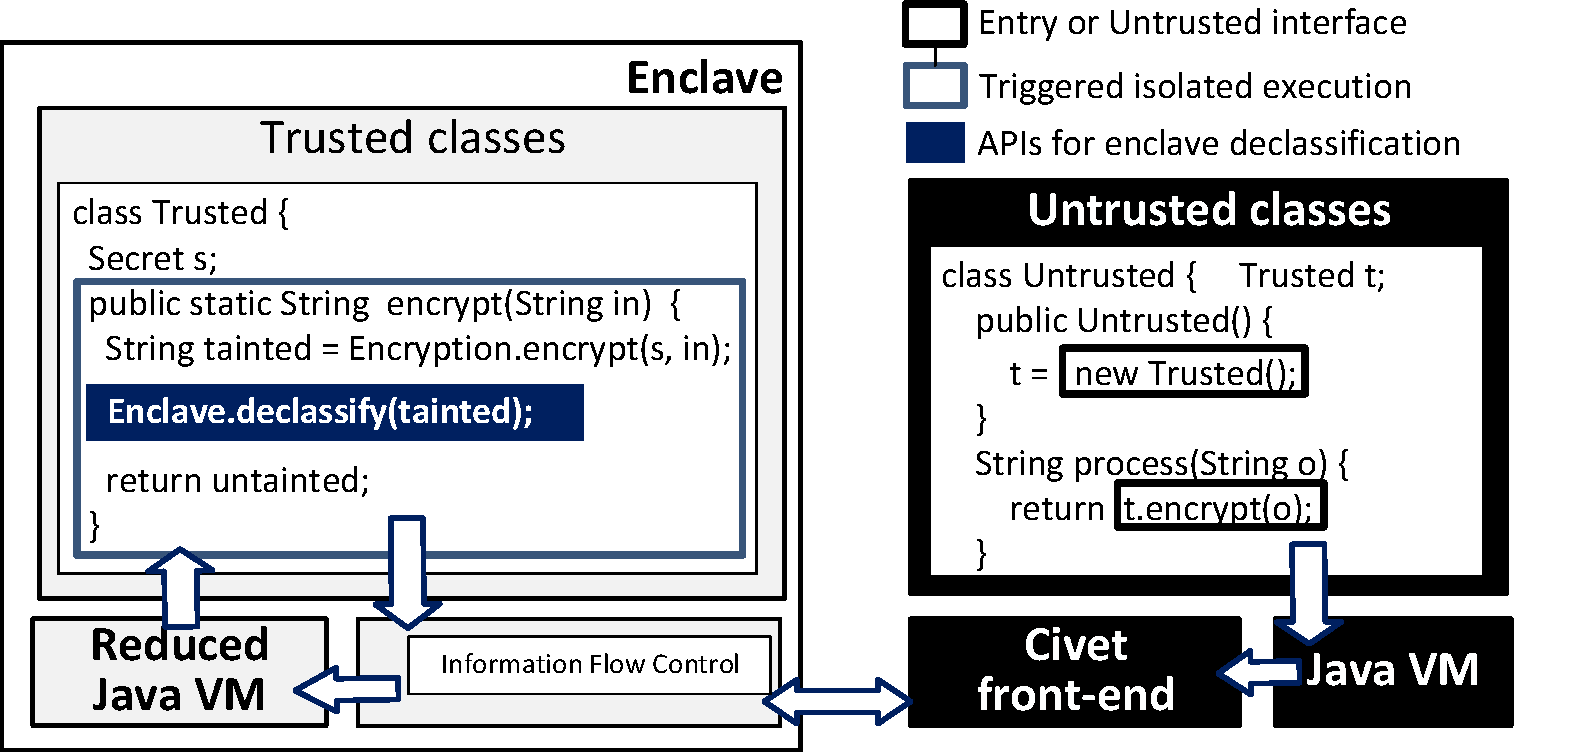
\includegraphics[width=1.0\linewidth]{declassify.pdf}
\footnotesize
\caption{How \sysname{} provides a declassifier API to declassify sensitive  data.
When the untrusted class ({\tt Untrusted}) from Figure ~\ref{fig:synthesis} now calls the {\tt encrypt} method of a trusted class ({\tt Trusted}),
\sysname{} automatically calls the {\tt encrypt} method inside enclave, and pass the {\tt byte[]} input.
Before returning, {\tt Trusted.encrypt} uses {\tt declassify()} to release the cipher generated and tainted  by {\tt cipher.doFinal()}.}
\label{fig:declassify}
\end{figure}

%Because the code running in enclave has access to complete address space, including the trusted as well as untrusted memory regions, it is easy for the trusted code to inadvertently undermine \sgx{} protection by writing secret information in the untrusted region. Further, leaking any information derived from or related to the secret may be used by the untrusted code to guess the value of secret information. For example, even in the presence of memory protection, sandboxing and virtualization, it is possible to recover the secret key used by crypto algorithms~\cite{kocher1996timing,osvik2006cache,weiss2012cache, zhang2012cross}. So, to ascertain the secrecy of the sensitive data, no information derived from the secret should exit enclave in plaintext.

%We use JAVA tool phosphor source and sink to taint provisioned data and control leakage
%\sysname{} leverages extensive research on information flow tracking and control in \java{} to harden the \sgx{} security. 

In the enclave, we implement source-to-sink taint tracking, using the open-source Phosphor library~\cite{phosphor}.
%\fixmedp{check this}
The programmer manually selects the classes containing secret data that take secret input from a remotely-provisioned source.
This taint is propagated to any new variables that result from explicit or implicit flows from a secret object.
The only way to remove taint from an object is to pass the object through a \sysname{} declassifier API,
which returns an untainted copy of the object.

%\fixmedp{Would be nice to have a simple example class with a label and declassifier in a figure, if space and time allow}

\sysname{} enforces the policy that only untained data may be returned from an enclave.
If tainted data is being returned, the system transparently encrypts the data and removes its taint before letting the data leave the enclave.
In the cases where a developer wants to return references to sensitive data, \sysname{} instead returns an opaque reference or, in the case of a literal, encrypts the return value.

%mFor tainted data, the developer may opt to either throw a runtime error, or, by default, to return an encrypted object instead.
%The en

% to taint the secret data when provisioned and propagate the taint to any new data generated as an explicit or implicit result of the secret data. We specify the enclave exit points as targets and enforce the policy that any tainted data must pass through a declassifier, that encrypts the data before egress. We only consider the provisioned data as security sensitive, as the enclave image is only integrity protected.

%Declassifier API: correct usage and scenarios
The \sysname{} framework provides a {\tt declassify(Object)} API that creates an untainted
copy of the object.  In practice, we expect this function to be used in conjunction with tests
on the returned data, or cryptographic functions to protect the data in transit across an untrusted channel.

Continuing our example from Figure~\ref{fig:synthesis}, in Figure~\ref{fig:declassify}, if the {\tt Untrusted} class wants to call the {\tt encrypt} method on the trusted object {\tt t}, \sysname{} front-end transparently passes the argument string {\tt o} to the enclave, and the corresponding {\tt encrypt} method is called in the enclave. The secret {\tt s} is tainted because it was provisioned from remote trusted server as shown in Figure ~\ref{fig:synthesis}. As a result, the call to method {\tt encrypt} of class {\tt Encryptor} taints the encrypted output string {\tt tainted}. If the developer had returned this {\tt tainted} variable, the \sysname{} information flow tracking would re-encrypt the ciphertext, and thus make the return value useless for the {\tt Untrusted} class. However, as the developer wants to return the ciphertext as is, she can declassify the {\tt tainted} string by passing it through the declassifier API to get an untainted version of the same object. Such untainted objects can be released from the enclave without further encryption.

%to let the application developer explicitly indicate that the argument object does not contain any secret information, and is safe to leave the enclave as is. For instance, if the enclave code encrypts a blob of data using the tainted secret provisioned key, the information flow will taint the encrypted data. However, because the encrypted data is safe to exit enclave if a perfectly secure encryption algorithm is used, the developer can explicitly mark the encrypted data as declassified. We note that the developers need to be extra careful while declassifying objects to inadvertently leaking secret information.

%Dealing with confidential code
%In order to protect the confidentiality of sensitive code,
%\sysname{} also allows classes themselves to be tainted.
%\sysname{} enforces a policy that any data returned from sensitive code is tainted, and the developer needs to explicitly declassify tainted output data to mitigate
%concerns around reverse-engineering the code based on brute-force probing of its outputs.
%Of course, the binary code itself is also not allowed to be copied out of the enclave.

% expose it to the untrusted world.
%The {\em code confidentiality} property of \sysname{} loads and executes encrypted classes from remote hosts to protect secret algorithm. We consider this provisioned code as equally security sensitive as provisioned data. ~

%\begin{table*}[t!b!]
\centering
  \begin{tabular}{p{0.05in} >{\raggedright\arraybackslash}p{2.05in} >{\raggedright\arraybackslash}p{4.4in}}
  \toprule
  \multicolumn{2}{l}{\it Security guarantees or features} & {\it The modeling approach applied by \sysname{}} \\
  \midrule
  \midrule
  \multicolumn{3}{l}{\bf Natively provided by the \sgx{} hardware (including the SDK):} \\
  \midrule
  & Isolating security-sensitive components &
  Asking developers to identify multi-level sensitivity, by marking the {\em entry classes}. Complete separation between isolated and untrusted classes.
  \\
  \midrule
  & Secure entry / exit of enclaves &
  Exporting public methods of isolated classes. Arguments are type-checked.
  \\
  \midrule
  & Integrity of the execution environment & 
  Packaging all supporting classes into a signed JAR.
  \\
  \midrule
  & Attestation \& secure provisioning & 
  Providing class {\tt Enclave}, to create secure channels and exchange attestation.
  \\
  \midrule
  \midrule
  \multicolumn{3}{l}{\bf Improvement from combining of \java{} language and the \sgx{} hardware protection:} \\
  \midrule
  & Memory safety \& control flow integrity &
  Naturally provided by \java{} language.
  \\
  \midrule
  & Reducing the enclave TCB &
  Automated partitioning based on class dependencies.
  \\
  \midrule
  & Preventing information flow leakage &
  Tracking information flow in trusted classes, only allow releasing the information if not tainted or declassified by developers.
  \\
  \midrule
  & Code confidentiality & Dynamically loading provisioned classes.
  \\
  \end{tabular}
  
\footnotesize
\caption{
The approaches applied by \sysname{} to model the security guarantees and features of the \sgx{} hardware, and to enhance the security by combining language and hardware protections.
}
\label{tab:features}
\end{table*}


%\input{Design of \jvm{} for \sgx{}}
%\section{The \thelibos{} Architecture}


The \libos{} of \graphene{}, or 
\thelibos{},
is a single library to be loaded beneath a Linux application,
as a compatible layer between
Linux \linuxapis{} and \thehostabi{}.
The purpose of \thelibos{} is to reuse an unmodified Linux application
upon an incompatible host OS or hardware.
%to support compatible OS features.
%for exporting compatible features.
An unmodified Linux application is built with the assumption of running on a Linux kernel or equivalent.
A Linux kernel
has exported a set of idiosyncratic features and characteristics,
or {\bf personality},
which an unmodified Linux application depends on.
%In order to reuse an unmodified Linux application
%on an incompatible host,
\thelibos{} takes the role of reproducing the Linux personality,
and is equivalent to a guest Linux kernel
over various host options.
%using \thehostabi{} exported by the host OS and PAL.
%The purpose of \thelibos{}
%is to resue an unmodified Linux application,
%by combining with a PAL and a host OS to behave as an equivalence of a Linux kernel. 
%%which is developed upon the assumption of running on a Linux kernel or equivalent.
%The main purpose of \thelibos{} is to reproduce
%the idiosyncratic features and behaviors of Linux,
%or the {\bf Linux personality},
%to resurrect Linux applications upon incompatible
%host OSes or hardware.
\graphene{} develops \thelibos{} as an ELF dynamic library (i.e., \code{\tt libLinux.so}),
loadable and linkable by a PAL.
%to be loaded on a host by the corresponding PAL.
%at the beginning of a \picoproc{}.


A key component of \thelibos{}
is a Linux system call table, which redirects \linuxapis{} from a Linux application to functions in \thelibos{}.
%a key Linux kernel component applications. 
%that \thelibos{} implements is the Linux system call table.
%For Linux and similar OSes,
A system call table is a primary entry point of a Linux kernel.
Each entry of the system call table
points to the kernel implementation of a Linux API related with a \linuxapi{} number (e.g., \code{NR\_open}).
%and triggers in-kernel operations for servicing requests from applications.
%and defines the interaction between applications and kernel.
\graphene{} moves the Linux system call table into \thelibos{},
and implements a number of \linuxapi{} handlers in the user space.
%The system call table in \thelibos{} contains a number of \linuxapi{} handlers,
Each \linuxapi{} handler emulates
individual \linuxapi{} that \graphene{} supports;
\graphene{} develops each handler
based on either a known specification, % known by the Linux application developers,
mostly described by a Linux manpage~\cite{linux-man-syscall},
or bug-for-bug behaviors
observed in a real Linux kernel.
For example, \syscall{rt\_sigaction} is partially documented
in the corresponding Linux manpage, and \thelibos{} implements the \linuxapi{} by mimicking the Linux kernel.
\graphene{} grows the functionality of \thelibos{}
primarily by extending the guest-level Linux system call table
with more complete \linuxapi{} implementation.

%Otherwise, for a few \linuxapis{} whose behaviors
%are not clearly defined by the Linux manpages,
%such as \syscall{rt\_sigaction},
%the \linuxapi{} handlers mimic the bug-for-bug behaviors of an actual Linux kernel.
%A continuing goal in \graphene{} is
%to extend \thelibos{} with more complete \linuxapi{} handlers.


%grow the functionality of \thelibos{},
%by extending the system call table with more complete handlers.




%The development of \linuxapi{} handlers in \thelibos{}
%is equivalent to implementing the specifications described in the Linux man pages~\cite{linux-man-syscall},
%including the valid inputs to each \linuxapi{},
%as well as the expected outcome.


%\paragraph{Implementing Linux Personality.} 
%\fixmedp{Revisit the logical flow of these paragraphs}
\Thelibos{} currently implements \graphenesyscallnum{} \linuxapis{},
and demonstrates 
the sufficiency of running applications ranging from servers to command-line applications.
For reference,
a relatively recent Linux kernel contains more than three hundred \linuxapis{}, including a long tail of infrequently-used \linuxapis{}.
%upon \thehostabi{}. % to interact with the host.
%Among the whole Linux \linuxapi{} table,
%A Linux kernel exports a long tail of infrequently-used \linuxapis{}.
%For reference, the Linux \linuxversion{} kernel exports \linuxsyscallnum{} \linuxapis{}.
A study of the Linux \linuxapi{} usage~\cite{tsai16apistudy}
indicates that only forty \linuxapis{} are indispensable to every applications available in the Ubuntu official repositories.
%The study also shows that
In the meantime, more than a hundred \linuxapis{} are used by only a single application,
or no application at all.
The development of \thelibos{} begins with
implementing twelve basic \linuxapis{} needed for running a ``hello world'' application,
such as \syscall{read}, \syscall{write}, and \syscall{open},
and then gradually grows the count of \linuxapis{}.
%for each new application introduced to run on \graphene{}.
As the count of \linuxapis{} continues to grow,
each time \thelibos{} is tested against a new application, the number of \linuxapis{} that need to be added
has dropped.
%Based on the types of applications priorized in \graphene{}, including servers, command-line programs, and language runtimes, some \linuxapis{} to be more important %for reusing the applications
%than the others. % \linuxapis{}.
According to the usage of each \linuxapi{} in applications,
developers can prioritize the popular \linuxapis{}, over other \linuxapis{} that are either unpopular among applications, or only used by administrative tools such as \code{reboot} or \code{ifconfig}.
\thelibos{} demonstrates that
\thehostabi{} is sufficient for implementing
a significant subset of the Linux \linuxapis{} to run
a representative sample of applications.


%The current \thelibos{} implementation
%includes a set of high-valued Linux \linuxapis{} for the types of applications
%that \graphene{} has targeted,
%including servers, command-line programs, and runtimes.
%The remaning \linuxapis{} may require extending \thehostabi{} with more privileged abstractions,
%including administrative operations
%and host-specific features.
%\thelibos{} demonstrates that \thehostabi{} is sufficient
%for exporting the host abstractions, to support a representative sample of Linux applications.

%such as memory sharing, scheduler configuration, and NUMA (non-uniform memory architecture) support.


%Linux exports a very long tail of infrequently-used \linuxapis{}.
%applications.




%An analysis indicates roughly 100 additional calls that can be implemented
%with the existing \pal{} ABI and coordination framework, less than 10 administrative calls that will not make sense to expose to 
%an application, such as loading a kernel module or rebooting the system, and roughly 54 that will require 
%\pal{} extensions to meaningfully implement, such as controlling scheduling,
%NUMA placement, I/O privilege, and shared memory.
%In the last category of system calls, the degree to which actual host details should be exported versus emulated is debatable.

%We believe represent the most commonly used system calls.
%When an application requests a call or argument that {\tt libLinux.so} does not implement,
%the picoprocess exits with a distinct error message. 
%Each time we have tested \graphene{} with a new application, the number of extra system calls
%required has dropped---most recently we only added 4 calls
%(namely, epoll\_create, epoll\_wait, semget and semop)
%to support the Apache web server.
%Thus, we believe \graphene{} implements a representative sample of Linux calls.

%such as {\tt sched\_setparam}, which manipulates scheduler-specific
%parameters or 
%{\tt uselib}, which has been abandoned 
%in {\tt glibc} version 2 in favor of a user-space dynamic linker.
%We do not plan to implement administrative interfaces, such as {\tt reboot}.
%The growth in the set of supported system calls has been driven by 
%the requirements of new applications we use to exercise \graphene{}, and has been 
%slowing considerably over time.



\subsection{\Linuxapi{} redirection}


\thelibos{} transparently intercepts \linuxapis{} in a Linux application. In a Linux kernel, a \linuxapi{} interrupt handler is assigned
to trigger the kernel operations,
whenever the application executes
a ``\assembly{syscall}'' or ``\assembly{int \$80}'' instruction.
The handler
performs a context switch from the application to kernel,
and redirects \linuxapi{} arguments to the kernel routine which services the requested \linuxapi{}.
%based on a kernel convention agreed by applications and Linux kernels.
\thelibos{} intercepts the \linuxapis{}
from an unmodified Linux executable or library, and redirects
to the system call table implemented inside \thelibos{}.
%intercepts the \linuxapis{}
%in an executable or library binary, and redirect the \linuxapis{}
%to the \linuxapi{} handlers inside \thelibos{}.
%\thelibos{} implements the callback functions for a subset of the Linux \linuxapis{}.
%For reference, Linux kernel \linuxversion{}
%has defined \linuxsyscallnum{} \linuxapis{} in total.


In normal cases,
\thelibos{} can redirect \linuxapis{} from an unmodified Linux application
using a modified C library (\libc{}).
%from an unmodified Linux application.
Most Linux executables and libraries avoid invoking \linuxapis{} directly,
but use \libc{} functions as wrappers to \linuxapis{}.
%which internally execute ``\code{syscall}'' or ``\code{int \$80}'' instructions.
%an executable or library in Linux and similar OSes invokes \linuxapis{} through \libc{},
%instead of directly containing the \code{syscall} instructions.
%The \libc{}
%contains a large set of \linuxapi{} wrappers,
%which encapsulate direct \linuxapis{} to the kernel as functions.
For example, the \libc{} function \funcname{read} is a wrapper to the \syscall{read} \linuxapi{},
which internally executes
the \assembly{syscall} instruction.
% that bares the same name and definition.
By defualt, \thelibos{} uses a modified
{\bf GNU C library (\glibc{})}~\cite{glibc},
since \glibc{} is compatible against most Linux applications released by Ubuntu. % are compatible against \glibc{}.
%which is compatible against most of the Linux applications released for Ubuntu.
%Other \libc{} variants, ,
%which are either fully or partially compatible with \glibc{},
%can be also modified to redirect \linuxapis{} to \thelibos{}.
%are alternatives upon \thelibos{} as long as they are modified for .
\graphene{} can also use other \libc{} variants,
such as \projname{uClibc}~\cite{uclibc} and \projname{musl}~\cite{musl},
if the application requires less \libc{} functionality.
%\graphene{} demonstrates that 
%are also demonstrated
%to be acceptable alternatives,
%with slight modification for \linuxapi{} redirection.




\graphene{} restricts the modification in \glibc{}
to up to \gipclines{} lines of code.
The C source code in \glibc{} consistently uses a platform-independent macro,
%referenced a single macro called
\funcname{INLINE\_SYSCALL},
to invoke \linuxapis{} to the kernel.
%when it needs to invoke a \linuxapi{}.
\funcname{INLINE\_SYSCALL} contains a piece of assembly code
that copies \linuxapi{} number and arguments to registers,
and then uses \assembly{syscall} to enter a Linux kernel.
\graphene{} modifies \funcname{INLINE\_SYSCALL}
to redirect a \linuxapi{} to
an entry point of \thelibos{} called \funcname{syscalldb}.
\funcname{syscalldb} saves the current register state, similar to a context switch,
and then
calls the \linuxapi{} handler
indicated by the \linuxapi{} number.
%, to trigger operations inside \thelibos{}.
For assembly code in \glibc{},
\graphene{} replaces each \code{syscall} instruction with
a dynamic call to
\funcname{syscalldb}, given the address of \funcname{syscalldb} is dynamically determined.
Figure~\ref{fig:libos:syscall-redirection} summarizes the mechanism of \linuxapi{} redirection.
%to \thelibos{}.


\begin{figure}[t!]
\centering
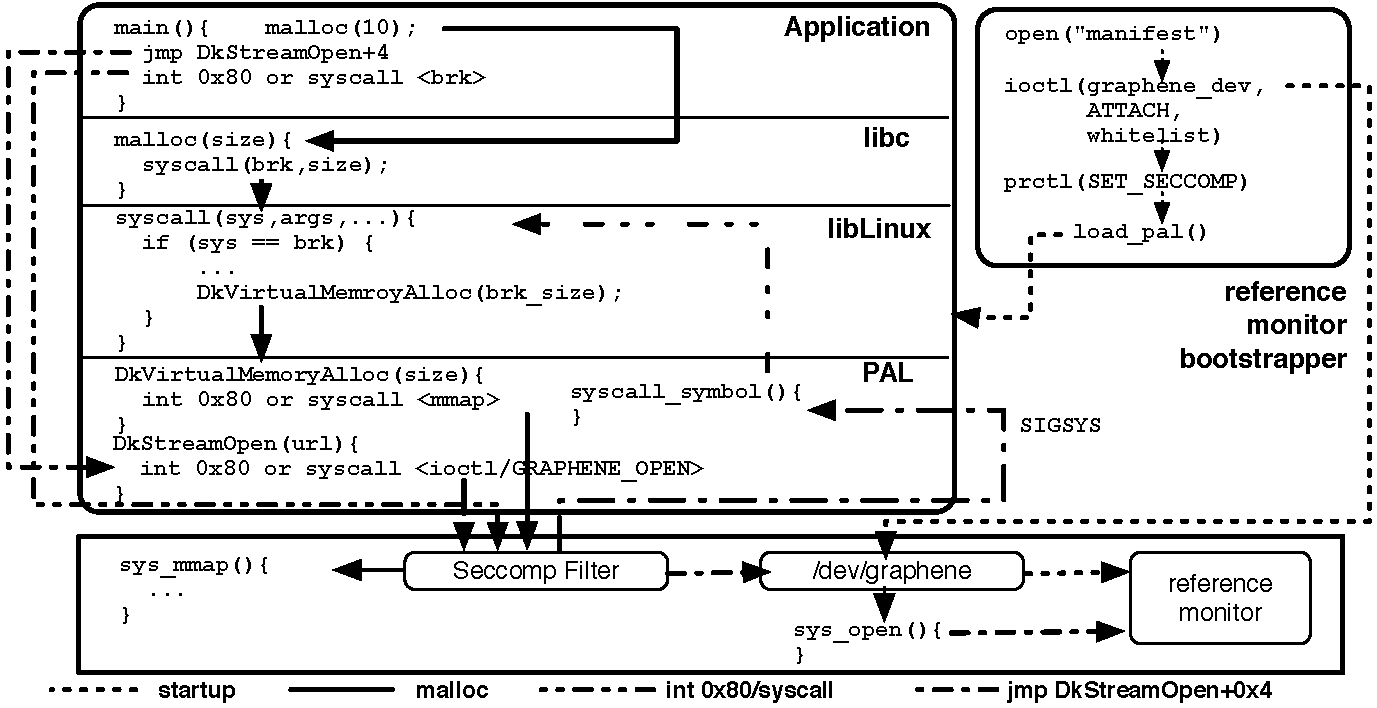
\includegraphics[width=\linewidth]{syscall-redirection.pdf}
\footnotesize
\caption{System call redirection for \thelibos{}.
In the normal case (first line of {\tt main}), {\tt malloc} is invoked causing the invocation of {\tt brk} ({\tt libLinux}) and {\tt mmap} in the \pal{}. In the second line, the application jumps to an address in \pal{}, which is permissible.
Files are accessed through {\tt ioctl} to {\tt /dev/graphene} and checked by reference monitor.
The third line invokes {\tt brk} with an {\tt int} instruction, which is redirected to the {\tt libLinux} function.}
\label{fig:libos:syscall-redirection}
\end{figure}


\graphene{} modifies several \glibc{} libraries with individual purposes,
%When using \graphene{}, an application must be deployed with the modified \libc{} libraries,
including \code{ld.so}, \code{libc.so}, \libpthread{}, and \libdl{}.
\Glibc{} partitions its code into separate libraries to reduce the binary sizes
loaded by each application.
%Despite that \glibc{} has partitioned its code into separate libraries,
\graphene{} only modifies the libraries which contains direct \linuxapis{} (i.e., \assembly{syscall} instructions).
%not every libraries of \glibc{} need to be modified for \linuxapi{} redirection.
%Only \code{libc.so}, \libpthread{}, and \libdl{} have included \code{syscall} instructions,
%and thus have to be modified for \graphene{}.
Other \libc{} libraries, such as \code{libm.so},
never directly invoke \linuxapis{} and only rely on 
existing \libc{} functions;
therefore, \graphene{} leaves \code{libm.so} and other similar \libc{} libraries unmodified.



\paragraph{Hard-coded \linuxapis{}.}
A static binary, or a platform-dependent application, may contain hard-coded \assembly{syscall} instructions
that cannot be redirected by a modified \libc{}.
Some application developers choose to statically link an executable against \libc{},
as a static binary with hard-coded \linuxapis{}. %\code{syscall} instructions.
Other application developers may program an application---usually a language runtime (e.g., go runtime) or system software (e.g., \projname{busybox})---with assembly code that directly invokes
platform-depenedent,
rare \linuxapis{} that are not wrapped by \libc{} functions.
%one of the \linuxapi{} wrappers in \libc{}, or \funcname{syscall}.
%As a result, a ELF binary may contain hard-coded \assembly{syscall} instructions.
%Either way leads to hard-coding \code{syscall} instructions in the ELF binaries.
Because modified \glibc{} does not redirect hard-coded \linuxapis{},
the \linuxapis{}
trigger context-switching into the host kernel,
causing security and compatibility issues as
exposing unauthorized, or unsynchronized host resources and states to the application.


As a solution,
\thelibos{} depends on host-level \linuxapi{} restriction to redirect hard-coded \linuxapis{}.
%to prevent \linuxapis{} from anywhere other than a PAL.
A direct \linuxapi{} traps into the host kernel,
unless the host has virtualized the interrupt handler to the \libos{}.
\graphene{} depends on each host to
detect unauthorized \linuxapis{} either from a wrong code location or with an unexpected \linuxapi{} number.
On Linux or a similar OS, the PAL can install a \linuxapi{} filter,
such as SECCOMP filter~\cite{seccomp}.
On some architecture, there are architectural limitation;
for example, SGX forbids \linuxapis{} inside an enclave and triggers an exception for an in-enclave \linuxapi{}.
%\code{syscall} instructions
%(e.g., SGX restriction).
%The details of the \linuxapi{} restriction mechanisms are discussed in
%\fixme{update labels}
%Section~\ref{sec:linux:syscall} and Section~\ref{sec:sgx:syscall}.
\thehostabi{} specifies that the host captures unauthorizes \linuxapis{}
and redirects to an exception handler (set up by \palcall{ExceptionSetHandler}).
%If a binary makes an illegal \linuxapi{},
%the host-level \linuxapi{} restriction will trigger an \code{ILLEGAL} exception
%at \thehostabi{},
%and thus the \linuxapi{} is redirected by an exception handler
%assigned by \thelibos{}.
The exception handler 
retrieves the \linuxapi{} number and arguments
from the saved context,
runs the \linuxapi{} handler,
and eventually pushes the return value back to the saved context. %\code{RAX} register.


Redirecting \linuxapis{} based on exceptions
can be expensive,
due to the overhead of context-switching between the host and guest.
Whenever an application invokes a direct \linuxapi{},
it traps into the host kernel, and then returns to the \libos{} to handle the \linuxapi{}.
Therefore, the process of redirecting a \linuxapi{} includes at least two times of context-switching, which can take up to microseconds.
To bypass the overhead,
\thelibos{} can 
rewrite the binary at run-time to redirect the hard-coded \linuxapis{};
%use {\bf binary translation} to modify the hard-coded \code{syscall} instructions;
\thelibos{} can
either scan-and-rewrites the whole binary at loading time,
or rewrites a single \assembly{SYSCALL} instruction in the exception handler.
%binary translation
%can be triggered when a host-level exception is raised
%for an illegal \linuxapi{},
%to optimize consecutive \linuxapi{} invocation at the same location.
%\thelibos{} can also perform a full scan in application binaries
%to spot and modify hard-code \code{syscall} instructions.
\graphene{} leaves the implementation of binary rewriting
as future work.



%\section{Automatic Partitioning of JAVA Applications}
\label{sec:partitioning}
\sysname{} reduces the TCB of a security critical 
application by automatically partitioning the 
application into trusted and untrusted parts. It is not 
easy for a novice developer to find the right 
partitioning boundary. As a result, the developer may 
include classes, which are not necessary for operation, 
in the trusted part. These extra classes may expose new 
attack vectors, reducing the security of the enclave. 
\sysname{} provides an enclave image utility to help 
the developer partition the code with minimum effort. 
The developer only needs to identify the classes that 
represent the secure objects.

The enclave image utility calculates the transitive 
closure of dependencies of the secure object classes.
The tool traverses all the imported classes by secure 
classes and marks them as secure too. The tool keeps 
traversing the newly added secure classes until there 
is no new class to be marked secure. It not only 
follows the user-defined classes but also the system 
classes to create a list of all the secure classes.

The utility then replaces the references of secure classes in the untrusted part with proxy stubs to make a remote method call instead of direct method invocation. The tool uses Phosphor information  flow tracking library to instrument the secure classes so that the information flow can be tracked at runtime as explained in Section ~\ref{sec:info-leak}. The output of the tool is an instrumented secure classes JAR and another JAR containing untrusted code with proxy stubs.

The enclave image tool then packages the Graphene LibOS, JVM, JNI, and the instrumented trusted JAR together, and generates the enclave object by cryptographically signing the package using its private key and \fixmebj{XX} algorithm. The untrusted JAR and the enclave object are deployed together in the cloud machine with \sgx{} capability. 

Thus, the automatic partition tool reduces the attack vectors exposed in the enclave, and removes the burden of the developer to create the partition boundary by finding the entry/exit points. This enforces a strict smallest possible TCB for the secure application.

%\papersection{Security isolation}
\label{sec:linux:security}

\issuedone{1.1.d}{Describe the security isolation story for Linux hosts}
\graphene{} separates OS features from security isolation.
This section explains the Linux host design for isolating mutually untrusting applications, with a reduced attack surface for protecting Linux kernels.
The discussion starts with the security guarantees and threat model, followed by the technical details of security isolation on a Linux host.



\papersubsection{Goals and threat model}

The security isolation model of \graphene{} ensures that mutually-untrusting applications cannot interfere with each other.
A goal of \graphene{} is to provide security isolation with comparable strength as
running applications in separate VMs.
When running two unrelated applications on the same machine,
the security requirement
of the OS involves not only blocking unauthorized access under normal circumstance,
but also preventing an application
from maliciously exploiting OS vulnerabilities to attack the other application.
Because a modern OS, such as Linux or \win{}, contains a rich of features and APIs,
it is difficult to eliminate OS vulnerabilities
or even just to verify whether an OS contains any vulnerabilities. 
A Linux container~\cite{lxc}
does provide a separate OS view for each application,
but still relies on the correctness of the whole Linux kernel to enforce security isolation.
On the other hand, a VM or a \libos{}
isolates the whole OS kernel or a part of the kernel in an unprivileged guest space
for each application.
The security isolation model prevents
any vulnerabilities inside the VM or the \libos{} from compromising the host kernel and other applications.



\graphene{} enforces security isolation %between applications
by separating 
backward-compatible OS features from security mechanisms.
A Linux kernel exports a wide range of system calls,
either as a legacy of previous kernels or as new programmability features. % of newer kernels.
By implementing OS features in a \libos{},
\graphene{} reduces the attack surface of a Linux kernel
to a small amount of system call corner cases.
%to implement \thehostabi{}.
%If a machine only runs applications in \graphene{},
%a Linux developer can try to carve out a minimal Linux kernel, containing only features needed by the Linux PAL.
A reduced attack surface
eliminates majority of execution paths inside a Linux kernel in which a malicious application can explore for vulnerabilities.
The complexity of Linux features and APIs exported by a \libos{} is unrelated with the attack surface of the host kernel,
unless the \libos{} asks for additional \hostapis{}.
A Linux developer can even carve out a minimal Linux kernel with only the features needed by the Linux PAL,
similar to shrinking a Linux kernel to a microkernel.
Otherwise, \graphene{} depends on the host security mechanisms to restrict a \libos{} from accessing unauthorized system calls and resources upon an unmodified Linux kernel.





The Linux PAL installs a {\bf system call filter} and a {\bf reference monitor}
for restricting the system calls, files, RPC streams, and network addresses
accessed by a \picoproc{}.
The Linux PAL requires \hostsyscallnum{} system calls in total
for implementing both required and optional \hostapis{}.
A system call filter, such as the Linux \seccomp{} filter~\cite{seccomp},
can restrict the system call access of an application
to only a small subset of all the system calls, with additional constraints on the parameters and optional flags permitted for each system call.
%The system call filter
%forbids an application from invoking any system calls
%that will interfere other \picoproc{} or increase the risk of exploitation in the host kernel.
A reference monitor further examines the arguments of permitted system calls to restrict the host resources accessed by an application, based on security policies configured in a manifest file~\cite{hunt07rethink}.
The system call filter and the reference monitor
significantly limit the ability of an untrusted \graphene{} \picoproc{} to interfere with the rest of the system,
preventing the risk of exposing any unknown vulnerabilities
on a kernel path never exercised by the system call footprint of \graphene{}.



\graphene{} contributes a multi-process security model 
based on a {\bf sandbox},
or a set of mutually-trusting \picoprocs{} running inside an isolated container.
The reference monitor permits picoprocesses within the same sandbox
to communicate over RPC streams,
allowing the \libos{} to share and coordinate any states
to create an unified OS view.
If two \picoprocs{} belong to different sandboxes,
the reference monitor will block any attempt of connecting RPC streams
between the \picoprocs{}
The access control over RPC streams
enforces an all-or-nothing security isolation model:
either two \picoprocs{} are in the same sandbox and share all the \libos{} states; or they are separated in two sandboxes and share nothing.
Even though the \libos{} instance can span its state across multiple \picoprocs{},
a host kernel needs not to examine the accesses to shared \libos{} states, but still enforces security isolation between sandboxes.




Files and network addresses
are the only host resources allowed to be shared across sandboxes,
using well-studied, explicit rules.
For sharing files, the reference monitor restricts the file access of a \picoproc{}
within a few host file or directories,
creating a restricted view of the local file system
(close to Plan 9's unionized file system views~\cite{pike90plan9}).
The file rules
in a manifest are similar to the policies of a {\bf AppArmor profile}~\cite{apparmor};
for each permitted file or directory,
a developer specifies the URI prefix and the permitted access type, either as read-only or readable-writable. %, within the target file or directory.
For sharing network addresses,
the reference monitor restricts a \picoproc{} from connecting through a local address or connecting to a remote address,
using {\bf iptables-like firewall rules}~\cite{iptablesman}.
Each network rule in a manifest
specifies the local or remote IP address and port range that a \picoproc{} is permitted to bind or connect a network socket.
The rules in a manifest file
specify a minimal list of files and network addresses that a \picoproc{} needs to access, and are largely based on existing security policies (e.g., AppArmor profiles, firewall rules).





\paragraph{Threat model (details).}
When running on a normal Linux host (without \sgx{} or other security hardware), \graphene{} assumes a trusted host kernel and reference monitor.
All the components inside the kernel space, including the \code{gipc} kernel module for bulk IPC, and the reference monitor,
are fully trusted by the other parts of the host kernel and the \graphene{} \picoprocs{}.
%which mediates all system calls with effects outside of a picoprocess's address space,
%such as file {\tt open} or network socket {\tt bind} or {\tt connect}.
On the other hand,
the host Linux kernel does not trust the \picoproc{}, including the Linux PAL, a \thelibos{} instance, \glibc{}, and the application.
The system call filter and reference monitor
initialized before an application starts running
defend the whole host kernel from malicious system calls invoked by a \picoproc{}.



All the components running within a \picoproc{}, including the Linux PAL, the \libos{} (\thelibos{}), \glibc{} libraries, and the application,
mutually trust each other. %, because all these components
%execute in the same guest address space.
Without internal sandboxing, the Linux PAL or \thelibos{}
cannot protect its internal states or control flows from an application.
Although some scenarios might require protecting the PAL or \thelibos{}
from the application,
\graphene{} only restricts the adversary
within a \picoproc{};
in other word, an adversary
only compromises the \libos{} in the same \picoproc{},
but can never interfere the host kernel 
or other unrelated \picoprocs{}.



For a multi-process application,
\graphene{} assumes that the \picoprocs{} 
%launched by the same application instance
running inside the same sandbox
trust each other and that all untrusted code run in sandboxed \picoprocs{}.
\graphene{} assumes the adversary can run arbitrary code inside
one or multiple \picoprocs within a sandbox.
The adversary can exploit any vulnerabilities in the \libos{}
or IPC protocol,
to propagate the attack to other \picoprocs{}.
\graphene{} ensures that
the adversary cannot interfere with any victim \picoprocs{}
in a separate sandbox.
A sandbox strictly isolates the coordination of \thelibos{} instances;
%if the only shared kernel abstractions are byte streams and files, 
the reference monitor ensures
that there is no writable intersection between sandboxes, so that
the adversary cannot interfere with any victim \picoprocs{}.


%%% The only processes allowed to run as standard kernel processes (non-\graphene{}) 
%%% are the reference monitor and
%%% system administration utilities that need more kernel interfaces than the \pal{} ABI provides.
%%% Ensuring that a collaborating picoprocess correctly implements
%%% some function (such as receiving a signal),
%%% as well as preventing exploitation of vulnerabilities in picoprocesses
%%% are beyond the scope of this work.

\graphene{} reduces the attack surface of the host Linux kernel, but does not change the trusted computing base; however, reducing the effective system call table size of a \picoproc{} does facilitate adoption of a smaller host kernel.
This thesis leaves the creation of a smaller host kernel for future work.

\papersubsection{System call restriction}
\label{sec:linux:security:syscall-restriction}


\graphene{} reduces the host ABI to \palcallnum{} calls
and the Linux system call footprint to \hostsyscallnum{} system calls.
To reduce the effective attack surface to a Linux host,
the Linux host restricts a \picoproc{} from accessing any system calls that are not part of the ordinary footprint of a Linux PAL.
The system call restriction on Linux focuses on blocking most of the system calls
that interferes with other processes.
The remaining permitted system calls with external effects are checked by 
the reference monitor (see Section~\ref{sec:linux:security:ref-monitor}).
 
%% dp: Meh
%%% Any picoprocess implementation 
%%% must restrict access to the host system call table,
%%% generally by blocking system calls in the host kernel~\cite{porter11drawbridge}
%%% or using {\tt ptrace}~\cite{xax}.


%The \pal{} is a host-provided library which implements \palcalls{} generic kernel ABIs,
%implemented using 
%These native system calls include {\tt ioctl} with 5 opcodes exclusively used by \graphene{} kernel extensions.

%This section describes how we adapt recent Linux sandboxing techniques 
%to \graphene{}.


%all allowed system calls with potentially external effects.

%%% For instance, an attempt to open a file will be checked by the reference monitor
%%% to see if the file is included in the sandbox definition, specified in the manifest
%%% with required permissions.
%%% Once the file handle is open, the \pal{} is then allowed to issue an {\tt mmap} or {\tt read}
%%% on the handle, as this operation can only affect the picoprocess address space
%%% or  file, which was already checked.

%Because the \pal{} is in the same address space as the application code, it is not
%trusted to enforce any security policies, and our threat model assumes that
%the \pal{} can be compromised by the adversary.
%Thus, the host kernel 
%only permits system calls that appear in the \pal{}'s source code and, through the reference monitor, further inspects calls that can have external effects.

%\begin{figure}[t!]
%\centering
%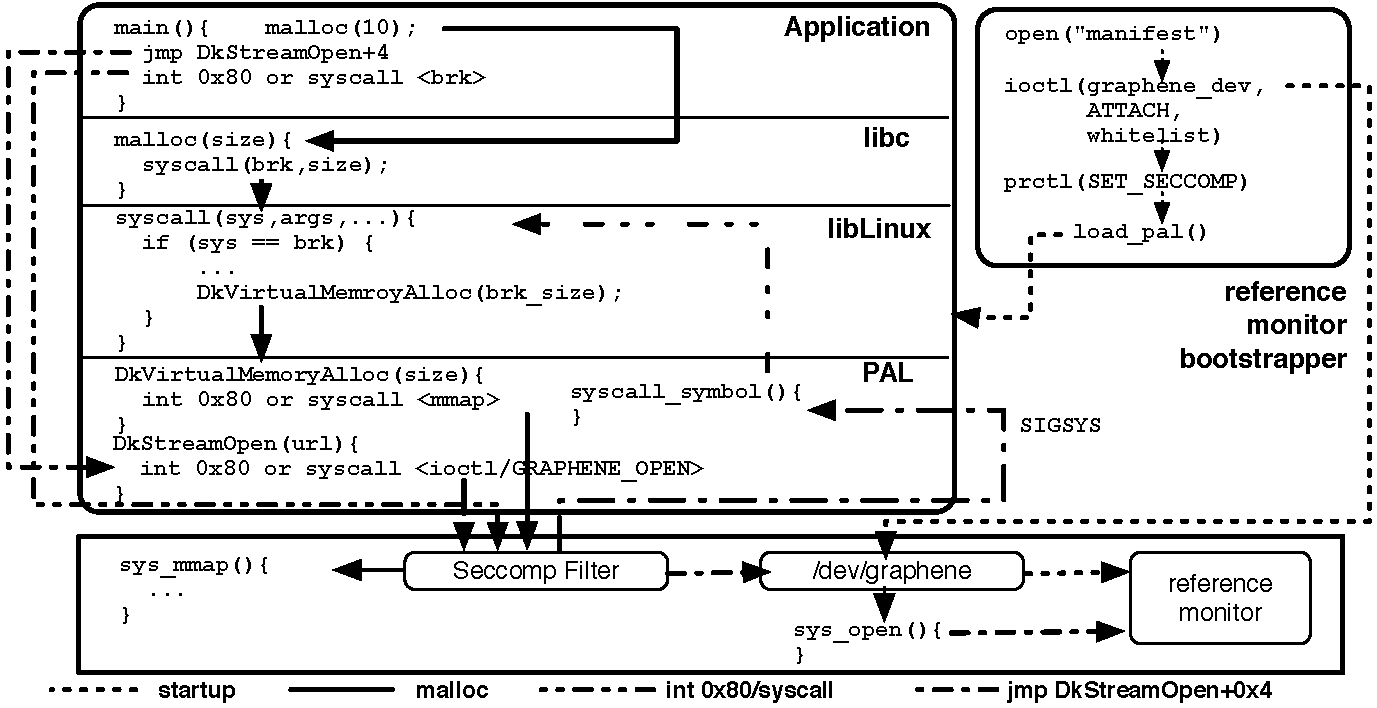
\includegraphics[width=\linewidth]{syscall-restriction.pdf}
%\footnotesize
%\caption[System call restriction approach in sysname{}]
%{System call restriction approach. The reference monitor loads policies into the LSM at startup.  A \graphene{} application requests OS services in three different ways. 
%In the normal case (first line of {\tt main}), {\tt malloc} is invoked causing the invocation of {\tt brk} ({\tt libLinux}) and {\tt mmap} in the \pal{}. In the second line, the application jumps to an address in \pal{}, which is permissible.
%Files are accessed through {\tt ioctl} to {\tt /dev/graphene} and checked by reference monitor.
%The third line invokes {\tt brk} with an {\tt int} instruction, which is redirected to the {\tt libLinux} function.}
%\label{fig:graphene:syscall-restriction}
%\end{figure}



\issuedone{1.3.d}{Extend the discussion of \seccomp{} filter}
\graphene{} restricts the host system calls 
using a \seccomp{} %(SECure COMPuting)
filter~\cite{seccomp}, a feature introduced in Linux 2.6.12.
% a recent Linux system call filtering mechanism, called 
A \seccomp{} filter allows a Linux process to install an immutable Berkeley Packet Filter (BPF) program
that specifies allowed system calls, as well as specifies
the consequence of invoking certain system calls, such as creating a \code{ptrace} event or raising a \code{SIGSYS} signal.
The BPF grammar is rich enough to filter scalar argument values,
such as only permitting specific opcodes for \syscall{ioctl},
as well as filter certain register values, such as blocking system calls from program counters (i.e., \code{RIP} register values) outside of the Linux PAL.
%This feature is particularly salient in the case of {\tt ioctl},
%where the \pal{} uses 5 out of over 400 opcodes for our bulk IPC module and sandbox creation;
%our BPF rules will block any other {\tt ioctl} opcode.
The current \seccomp{} filter installed by the Linux PAL contains \seccomplines{} lines of straightforward BPF macros.  %Experiments show that adding more precise argument checks has no significant impact on system call latency.
Once a \seccomp{} filter is installed in a process,
the filter intermediates
every system calls from the process and its future children, and guarantees the processes can never bypass the restriction.
The Linux PAL uses \code{SIGSYS} signals to capture rejected system calls,
and can either terminate the whole application or
redirect the system call to \thelibos{}.
The consecutive steps of system call redirection are described in Section~\ref{sec:libos:syscall-redirection}.



Developing a \seccomp{} filter presents several technical challenges.
First, a filter must restrict consecutive \picoprocs{}
to install a new filter the reverts the system call restriction.
%A \seccomp{} filter is installed using the \syscall{prctl} system call, so
Blocking the \syscall{prctl} system call in a \seccomp{} filter will prevent further installation of \seccomp{} filters.
Second, the BPF grammar can only filter certain values or ranges of a register.
The filter needs to
ensure that only the Linux PAL can invoke system calls;
however,
for satisfying the dynamic loading behavior of \thehostabi{},
the Linux PAL
is built as a shared library loaded at an address randomized by the Linux ASLR (Address Space Layout Randomization) feature.
If a filter only permits a specific range of program counters,
a child \picoproc{}
will load the Linux PAL at another randomized address,
and the inherited filter will restrict the child \picoproc{} to invoke any system calls.
The Linux PAL introduces a small, initial loader
loaded at a fixed address
within each \picoproc{} and permitted to invoke system calls.
Finally, a \seccomp{} filter
cannot check a string argument, such as a file path for \syscall{open} or a network address for \syscall{bind}.
Checking a string argument requires
involves reading user memory of unknown sizes and string comparison, and the BPF grammar only allows checking an argument arithmetically.
Filtering permitted file paths and network addresses
must rely on a trusted reference monitor (see Section~\ref{sec:linux:security:ref-monitor}).
%In order to avoid the overhead of trapping to the reference monitor on 
%every use of {\tt open}, {\tt stat}, {\tt bind} or {\tt connect} system calls, we instead 
%force picoprocess to only use {\tt ioctl} system call to \graphene{} special device ({\tt /dev/graphene}) as alternative interface these system calls. Direct access to these system calls are banned by seccomp filter.
%extend AppArmor~\cite{apparmor} 
%to enforce file system isolation in the kernel.



The \seccomp{} filter blocks  unauthorized system calls
from anywhere inside a \picoproc{}.
Even if none of the application binaries contains any \assembly{syscall} or \assembly{int \$80} instruction,
a piece of malicious application code can always bypass the Linux PAL
to invoke unauthorized system calls.
The application code can simply
jump to a \assembly{syscall} instruction inside the Linux PAL,
or corrupt a returned address on the current stack to launch a ROP (return-oriented programming) attack.
Even if the Linux PAL is hidden or isolated from the application,
an adversary can always leverage a gadget, a byte sequence that resembles the target instruction, within an executable or a library.
Therefore, the \seccomp{} enforces both program-counter-based 
and argument-based restrictions
to block unauthorized system calls from both the Linux PAL and the rest of \picoproc{}.


%In order to reduce the impact of bugs in the reference monitor,
%the reference monitor itself runs with a \seccomp{} filter, blocking unexpected system calls.


\paragraph{Security implications.}
Using an existing system call restriction mechanism like \seccomp{},
\graphene{} limits the ability of an untrusted application to attack a Linux kernel.
Ideally, since \thelibos{} only requires \thehostabi{},
\graphene{} can adopt a modified Linux kernel
that only exports \palcallnum{} \hostapis{} to each \picoproc{}.
%However, as a usability feature, \graphene{} runs \graphene{} on an unmodified Linux kernel using a Linux PAL to translate among host interfaces.
The \seccomp{} filter instead isolates a \picoproc{} on an unmodified Linux kernel,
with a reduced attack surface 
comparable to only exporting \thehostabi{}.
%The filter only permits \hostsyscallnum{} system calls with specific flags and opcodes
%required by the Linux PAL.
According to the principle of least privilege,
each component or layer in a system should only be granted access to a minimal amount of resources or abstractions
required for performing the expected tasks.
The \seccomp{} filter only permits
a minimal amount of system calls with specific flags and opcodes
required by the Linux PAL,
so an untrusted application
can only trigger
a limited amount of execution paths inside the host Linux kernel.
\graphene{} limits
the ability of an untrusted application to explore
known and unknown vulnerabilities
on any kernel execution paths for servicing one of the blocked system calls.



Although a regular Linux process can also leverage a \seccomp{} filter,
\graphene{} makes a major contribution
to reduce the system call footprint of any large-scale application
to a fixed, small system call profile.
Analysis %of applications and libraries
%in the official Ubuntu repositories
shows that the system call  footprint of a large-scale application such as Apache or MySQL can contain more than 100 system calls.
Since \thelibos{} has absorbed the Linux system call table,
running Apache, MySQL, or any other application in \graphene{} leads to at most \hostsyscallnum{} host system calls.
As a system
running a wide range of applications
can exposes a different partial view of the system call table to each application,
\graphene{}
has a static system call profile for all applications,
allowing OS developers to focus
on testing or analyzing a small portion of execution paths and corner cases
of a Linux kernel.
\citet{sun15unpredictability}
proposes sandboxing an uncertain, potentially-malicious application
in \graphene{}
with an unpredictable \thelibos{} implementation.







\paragraph{Static binaries.}
Besides security purposes,
a \seccomp{} filter provides a compatibility feature
for redirecting hard-coded system calls
in a statically-linked application binary.
\graphene{} leverages the \seccomp{} filter to redirect these leaked system calls
back to \thelibos{}. 
The filter contains BPF rules to check if the program counters
invoking the system calls
are parts of the Linux PAL.
The filter blocks system call invoked outside of the Linux PAL
and delivers a \code{SIGSYS} signal
to the PAL signal handler for redirecting the system calls to \thelibos{}.



\papersubsection{Reference monitor}
\label{sec:linux:security:ref-monitor}

The reference monitor on a Linux host
checks the arguments of host system calls for referencing any sharable host resources.
A host system call like \syscall{open}, \syscall{connect}, or \syscall{bind}
specifies a file system path or a network address
for opening a file or network stream and cannot be filtered by a \seccomp{} filter.
The host kernel trusts the reference monitor
to only permit
a list of sharable resources in a \picoproc{},
based on
rules in a manifest file.
Once the reference monitor has permitted the creation of a file or network stream,
consecutive operations on the stream
such as reading or writing data can be trusted
as long as being mediated by one of the permitted system calls.


\begin{figure}
\centering
\begin{lstlisting}
loader.exec = file:/usr/sbin/apache2        # allow loading executable 
loader.preload_libs = file:/graphene/libLinux.so    # loading libLinux
fs.allow_ro.libc = file:/graphene/libc/     # loading modified libc
fs.allow_ro.mods = file:/usr/lib/apache2/modules/   # loading modules
fs.allow_ro.cond = file:/etc/apache2/       # reading configuration
fs.allow_rw.logs = file:/var/log/apache2/   # writing to logs
fs.allow_ro.http_docs = file:/var/www/      # reading website files
net.allow_bind.httpd = 0.0.0.0:80           # binding to local port 80
net.allow_conn.any = 0.0.0.0:1-65535        # allow any connection
\end{lstlisting}
\caption{A example of a manifest file, containing security rules for the reference monitor to permit accessing sharable resources. The manifest file is for running a Apache http server (without php and other language engines).}
\label{fig:linux:manifest-example}
\end{figure}


The reference monitor enforces simple, white-listing rules
based on security mechanisms
already familiarized by users and developers.
Figure~\ref{fig:linux:manifest-example} shows an example of resource access rules
in a manifest.
First, a manifest lists
the URI prefixes of permitted files or directories
of an application,
similar to an AppArmor profile.
The executable (\code{loader.exec}) and the preloaded \libos{} binaries (\code{loader.preload\_libs})
are permitted for read-only access by default.
The reference monitor
simply compares file URIs against each permitted URI prefix
and checks the access types;
unlike many existing security mechanisms in Linux and similar OSes, such as permission bits, Access Control Lists (ACLs), and SELinux labels,
the reference monitor does not retrieve
security policies from file metadata, but obtains the manifest from an out-of-band channel.


Manifest-based security
simplifies the inspection, authentication, and population
of security policies.
An Android application is deployed with a similar manifest,
listing the accessed files and other resources,
which users approve when installing the application.
Developers can authenticate a security policy by signing the content of a manifest.
Moreover, to run an application, a user can choose among multiple manifest files
with different levels of security privileges.



Network rules in a manifest are similar to {\bf iptables firewall rules} for defending a server or a desktop machine.
A network rule specifies a local or remote address
that the application is permitted to bind or connect a network stream.
A local or remote address
can be an IPv4 or IPv6 address (possible to specify an ``any'' address, i.e., \code{0.0.0.0} or \code{[::1]}), combined with a specific port number or range.
When an application creates a network stream,
the reference monitor checks whether the local and remote addresses
match one of the network rules.







%is implemented using {\tt ioctl} system call to a special device {\tt /dev/graphene}.
%A picoprocess is restricted by seccomp filter~\cite{seccomp} to use any {\tt open} or socket {\tt connect} and {\tt bind} system calls.
%It must use the \graphene{} special device to open or create streams,
%so the file paths or network addresses can be checked against the sandbox rules.
%The kernel module as the driver of the \graphene{} special device can coexist with any LSM such as \emph{AppArmor} or \emph{SELinux}.

The reference monitor on a Linux host
is implemented as a Linux Security Module (LSM) extended from the existing AppArmor module.
AppArmor is the default LSM of most Linux distributions,
and a Linux kernel disallows multiple LSMs (e.g., AppArmor, SELinux) to be effective simultaneously.
\graphene{} instruments
a few security hooks of the AppArmor, to add checks for file system paths
and network addresses.
The security checks of the reference monitor are stackable with other host security mechanisms.
For example, if a manifest lists a root-privileged file and the \graphene{} application runs in a unprivileged process,
existing security checks in a Linux kernel
still blocks the file access even though the reference monitor permits the access.
The drawback of the implementation
is that \graphene{} must run on a modified Linux kernel.
Linux kernels do not support loading LSM as a dynamic kernel module.
\graphene{} only replaces
the AppArmor LSM in a Linux kernel; the rest of the Linux kernel remains unchanged.


A trusted security loader initializes the reference monitor
when launching an application in \graphene{}.
When a user launches an application in \graphene{} from the command line,
the first \picoproc{} begins in a new sandbox.
The security loader
reads the manifest file given by the user,
and submits the sandbox rules to the reference monitor.
The reference monitor exports a miscellaneous device called \code{/dev/graphene}
for the security loader to submit sandbox rules using the \syscall{ioctl} system call.
Once the reference monitor
starts a \picoproc{} in a sandbox, neither the first \picoproc{} nor any consecutive \picoprocs{} spawned in the sandbox can ever escape the sandbox or drop the restrictions on certain resources.


\paragraph{Alternative approaches.}
Other approaches can implement the reference monitor without modifying a Linux kernel, with a trade-off of performance or development simplicity.
An approach is to implement the reference monitor as a trusted process receiving \code{ptrace} events from \graphene{} \picoprocs{}.
Using the \syscall{ptrace} system call, this reference monitor can retrieve user memory from the monitored \picoprocs{},
and block the system calls which request for unpermitted resources.
Unfortunately, intercepting every system calls with \code{ptrace} events introduces significant overhead to \hostapis{};
thus, this approach is not ideal for isolating \graphene{} applications on a Linux host.


Another approach is to translate the resource rules in a manifest file
to AppArmor or iptables rules.
As explained in previous paragraph, the file and network rules in a manifest file are similar to the file lists in an AppArmor profile and the firewall rules enforced by iptables.
Instead of implementing a \graphene{}-specific reference monitor,
\graphene{} can convert a manifest file, either statically or dynamically,
to security rules recognized by AppArmor and iptables.
This approach requires no modification
in a Linux kernel, and can benefit from
existing optimizations of AppArmor and iptable. %these security mechanisms.
\graphene{} leaves the integration with AppArmor and iptables for future work.




\paragraph{Dynamic process-specific isolation.}
A child \picoproc{} may either inherit its parent's sandbox, 
or start in a new sandbox,
by either specifying a flag to \palcall{ProcessCreate} or calling the sandboxing \hostapi{}, \palcall{SandboxSetPolicy}.
A new sandbox may obtain a subset of the original file system view,
but can never request access to new regions of the 
host file system. 
%The restrictive policy enforced on the child will be written in a new manifest file generated by the parent, and the policy will be checked by the reference monitor.
If a child \picoproc{} voluntarily moves itself to a new sandbox
using \palcall{SandboxSetPolicy},
the Linux PAL issue another \syscall{ioctl} call to \code{/dev/graphene}
to dynamically detach
the \picoproc{}
from the parent's sandbox and update sandbox rules. The reference monitor
closes existing RPC streams and prevents RPC stream creation 
across sandboxes.
%among picoprocesses
%that are not in the same sandbox.
%and restricts external connections to remote URIs according to firewall rules in the manifest.
When a process detaches from a sandbox,
the reference monitor effectively splits the original sandbox
by closing any RPC streams that could bridge the two sandboxes.


\begin{comment}
We hasten to note that program counter filtering
is only provided for backwards compatibility, not security.
An attacker can compromise the \pal{}, so system policies are enforced
externally by the reference monitor.


Dynamically redirecting system calls to {\tt libLinux} is 
less efficient than dynamically linking against
the \graphene{} libc or statically compiling {\tt libLinux} into the application.
The overhead of dynamic redirection comes from 
transferring control to the kernel, then back to 
the \pal{}, and then to {\tt libLinux}.
We leave exploration of more efficient alternatives for future work,
such as redirecting the hardware system call table to {\tt libLinux}
on a host system like Dune~\cite{belay12dune},
or dynamically rewriting parts of the static binary~\cite{hunt99detours}.
\end{comment}

%\paragraph{Example.}
%Figure~\ref{fig:graphene:syscall-restriction} illustrates three possible situations. 
%%% An unmodified Linux application is dynamically linked against the 
%%% \graphene{} {\tt libc}, 
%%% which then dynamically links its system calls from {\tt libLinux},
%%% which in turn links in the host kernel ABI from the \pal{}.
%%% The application requests OS functionality in three ways.
%An unmodified application first invokes the {\tt libc} function {\tt malloc}, which issues 
%a {\tt brk} system call to {\tt libLinux}, which requests memory 
%from the host via a {\tt Dk\-Virtual\-Memory\-Alloc} \pal{} call,
%which ultimately issues an {\tt mmap} host system call.
%The {\tt mmap} host system call is allowed by seccomp because it only 
%affects the picoprocess's address space.
%The second line of the application jumps to the \pal{} instruction that issues
%an {\tt open} system call.
%From a security perspective, this is permissible,
%as it is isomorphic to \pal{} functionality.
%In practice, this could cause
%corruption of {\tt libLinux} or application data structures,
%but the only harm is to the application itself. 
%Because this system call involves the file system, the reference monitor LSM first checks if the file to be opened is included in the sandbox definition (manifest) before allowing  the {\tt open} system call in the kernel.  
%Finally, the application uses inline assembly to issue a {\tt brk} system call;
%%in an attempt to obtain I/O port privilege; 
%because this system call was not issued by the \pal{},
%seccomp will redirect this call back to the \pal{},
%which then calls the {\tt libLinux} implementation.


Sandbox creation in \graphene{} can provide
more options than virtualization, to reflect the security policy of applications at any timing,
in the granularity of picoprocess. 
A picoprocess can voluntarily detach itself from the current sandbox, dropping its privileges,
after finishing security-sensitive operations.
If a picoprocess decides one of its children is not trustworthy, it may also start the child under a restricted manifest,
or promptly shut down RPC streams to stop sharing OS states.
The picoprocess that moves to a separate sandbox will have a restrictive view of the filesystem, and no coordination with the previous sandboxes.
Section~\ref{sec:eval:graphene} describes an experiment that improves security isolation of Apache http server without sacrificing functionality.



%We add a \pal{} call which
%permits a picoprocess to request that it be moved into a new sandbox.
%This call, as well as file system path checks, are implemented
%as extensions to the  AppArmor LSM~\cite{apparmor}.
%%We modify \sandboxmodlines{} lines in the
%%to implement this call,
%The new sandbox call closes any open stream handles that cross sandbox boundaries;
%mediate path lookups;
%and create a new broadcast stream for multi-process
% coordination (\S\ref{sec:graphene:namespaces:blocks}).
%%The reference monitor also interposes on this call so that it can 
%%mediate future stream creation.

%To securely apply seccomp filtering we leveraged the fact that all
%\graphene{} processes have the same parent and also the new
%{\tt NO\_NEW\_PRIVS} bit introduced for Linux processes starting kernel
%version 3.5. This bit can be set by any process, is inherited across
%{\tt fork}, {\tt clone}, and {\tt execve}, and cannot be unset by
%children processes. Thus, we set the {\tt NO\_NEW\_PRIVS} bit in the initial
%\graphene{} process and apply seccomp filters allowing only system calls
%with corresponding functions in the \pal{}. As a result all \graphene{}
%processes will inherit the filters and cannot relax or bypass it.



%which reduces the kernel
%system call API surface to user-level processes. This mechanism allows
%a process to specify a whitelist filter for system calls, which is
%implemented as a Berkeley Packet Filter (BPF) program. The invocation
%of a disallowed system call causes the application to throw a {\tt SIGSYS}
%signal, which can be caught by a registered handler provided by the
%application. In \graphene{} we registered this handler at the \pal{}.


%\graphene{} applications rely on an OS loaded as a library to request
%system services. As most of traditional applications, \graphene{}
%processes do not normally issue system calls directly: they invoke
%wrapper functions from a \graphene{}-compliant version of libc, which
%allows for portability, security (parameters are limited and checked)
%and easiness of programming. However, while standard libc functions
%directly invoke the kernel system call themselves, our modified
%version of libc wrappers invoke functions from another library which
%represents the OS, libLinux (Figure \ref{fig:graphene:syscall-restriction}). A
%\graphene{} application can access all necessary system functionality
%through libLinux, which invokes corresponding system call functions at
%the \pal{}, also loaded as a library with a
%\graphene{} process. The \pal{} is the layer responsible for directly
%invoking system calls at the kernel. As discussed in \S\ref{sec:graphene:impl} the \pal{} provides \graphene{} applications with a
%subset of the kernel system call interface.\graphene{} applications rely
%on an OS loaded as a library to request system services.
%
%Even though we expect most of \graphene{} applications to leverage libc
%wrappers, we need to address applications that need to invoke system
%calls directly. Applications might need to bypass a library such as
%libc because some needed wrappers are not provided (there are no
%wrappers in libc for module and NUMA related system calls), or the
%wrapper does not meet the programmer’s needs. \graphene{} applications
%that need to perform direct invocation of system calls run unmodified
%as long as the system calls invoked are provided by the libos{l{}. We
%do not consider this a security violation; even though the application
%would be risking not functioning according to the libosaradigm for
%bypassing the \pal{}, all potential damage would be confined in the
%misbehaving application itself.  However, we do not allow the direct
%invocation of a system call that does not have a corresponding
%function in the libosnd \pal{}. In Figure \ref{fig:graphene:syscall-restriction}
%we illustrate these three situations. We have a \graphene{} application
%loaded with three libraries: a \graphene{}-compliant libc, libLinux
%representing the library OS with functions for a selected number of
%system calls, and the \pal{} which actually invokes host kernel system
%calls. The illustrated application requests three different types of
%OS functionality. It first invokes a function from libc, then it
%directly invokes a system call whose functionality is provided by the
%\pal{}, and third it attempts to directly invoke a system call not
%present in the \pal{}, which is not allowed by \graphene{}.

%We enforce system call restriction by leveraging seccomp Linux system
%call filtering mechanism~\cite{seccomp}, which reduces the kernel
%system call API surface to user-level processes. This mechanism allows
%a process to specify a whitelist filter for system calls, which is
%implemented as a Berkeley Packet Filter (BPF) program. The invocation
%of a disallowed system call causes the application to throw a {\tt SIGSYS}
%signal, which can be caught by a registered handler provided by the
%application. In \graphene{} we registered this handler at the \pal{}.
%
%To securely apply seccomp filtering we leveraged the fact that all
%\graphene{} processes have the same parent and also the new
%{\tt NO\_NEW\_PRIVS} bit introduced for Linux processes starting kernel
%version 3.5. This bit can be set by any process, is inherited across
%{\tt fork}, {\tt clone}, and {\tt execve}, and cannot be unset by
%children processes. Thus, we set the {\tt NO\_NEW\_PRIVS} bit in the initial
%\graphene{} process and apply seccomp filters allowing only system calls
%with corresponding functions in the \pal{}. As a result all \graphene{}
%processes will inherit the filters and cannot relax or bypass it.


%\begin{figure}
%\begin{centering}
%\includegraphics[width=2.0in\textwidth]{figures/syscall_restriction.png}
%\footnotesize
%\caption{System call restriction approach. \graphene{} application requesting OS services. The {\tt printf} function is handled by a wrapper function at our modified version of libc., which invoked a corresponding syscall function at libLinux, the library OS.This function invokes a system call function at the \pal{}, which actually invokes kernel system calls. The application also directly invokes two system calls and the last invocation is prohibited.
%\label{fig:syscall_restriction}
%\end{centering}
%\end{figure}

%\end{comment}

%\papersection{Seamless Provisioning of Secure Objects and Classes}
\label{sec:provisioning}

%\section{Framework Implementation}
\label{sec:implementation}

In this section we describe the design of \sysname{}.
\sysname{} adds language support in \java{} virtual machines to
create and execute partitioned applications in enclaves.

\subsection{Partitioned \java{} Execution}

To executed partitioned applications,
\sysname{} creates two worlds of \java{} execution,
one in an enclave and one outside the enclave,
to execute code at different security levels.
Each world contains an individual \java{} vM.
We allow only classes that are part of a signed enclave images to
be executed inside the enclave,
and all the other classes of the application
must run outside the enclave and access the secured classes through
an interface exported by the enclave.

Using \java{} language to implement enclaves
has the benefit of minimizing the development or porting cost.
Consider partitioning a native application for enclaves.
There are two primary sources of development or porting cost:
Separating the security-sensitive code from all the remaining code,
and designing the interface between the two.
%\java{} classes have huge advantage on fulfilling both goals
%with minimal works, for two reasons:
\java{} classes are well modularized and are natural granularity for partitioning.
Public methods can be exported as
enclave interfaces, with proper type-checking of arguments.

%\sysname{} allows \java{} applications
%to easily model enclave support as part of the language,
%without the awareness of the native interface to architecture.
%To reflect this concept, we have implemented two key principles in the language support:
%\begin{compactenum}
\sysname{} models each enclave as an object,
both inside and outside the enclave.
The object is used to access enclave information and features,
such as retrieving security attestation.
Instantiating and interfacing with the isolated classes
in enclaves is transparent to the untrusted part of application,
except the first instantiation.

%For the untrusted side of an application, both the enclave itself and
%the classes isolated in the enclaves
%are encapsulated as black boxes, to which the application
%can request for isolated execution seamlessly.
%These objects can be passed as parameters to other methods,
%or even overrode to extend their functionalities.

\begin{figure}[t!]
\vspace{-0.1in}
\centering
\includegraphics[width=3in]{civet-structure.pdf}
\vspace{-10pt}
\caption{\sysname{} framework overview. \sysname{} creates two worlds for an partitioned \java{} application, each with an individual JVM. The JVM in the enclave is ported using Graphene library OS. Untrusted classes can invoke methods of trusted classes through proxy objects, which will transparently access the enclave interface, through serialization and deserialization over an ring buffer accessed by both untrusted JVM and trust JVM. }
\label{fig:overview}
\end{figure}

\paragraph{Framework overview.} Figure ~\ref{fig:overview} shows the design and 
components of ~\sysname{} infrastructure.
All supporting classes to be isolated in the enclave
are packed into a JAR package --- an enclave image ---
and signed using a key given by the developers.
The untrusted side of the application initializes the enclave
using the enclave image JAR,
and starts to instantiate objects inside the enclave.
For each objects in the enclave, \sysname{} create a {\em proxy object} outside the enclave,
to access the interface exported from the enclave.
%and to represent the isolated objects to the rest of world.

The JVM running inside the enclave is a \jvmname{} VM
ported with the libOS-based programming model, using Graphene library OS.
Proxying isolated objects are handled through JNI in the untrusted JVM,
to access the low-level enclave interfaces.
To invocation of methods on the proxy objects are communicated
through a {\em ring buffer} outside the enclave memory,
accessible by both the enclave and the untrusted application.
The object ID, name of the invoking method, and all parameters are
serialized into binary forms and passed through the ring buffer.
In the enclave, one or more worker threads, initialized by the trusted JVM,
will poll the ring buffer,
accept the invocation requests,
de-serialize the parameters, invoke the method,
and return the result through the ring buffer.

%\begin{figure}[t!]
%\footnotesize
%\noindent
%\begin{minipage}[t]{.38\linewidth}
%\begin{lstlisting}[title=Isolated class,frame=none]
%class Secured {
%  Object run(
%    String args[]
%  ) {
%    ...
%  }
%}
%\end{lstlisting}
%\end{minipage}\hfill
%\begin{minipage}[t]{.54\linewidth}
%\begin{lstlisting}[title=Untrusted class,frame=none]
%class Untrusted {
%  static void main(
%    String[] args) {
%    Enclave e =
%      new Enclave(
%        "enclave.jar");
%    Secured o =
%      e.createInstance(
%        Secured.class);
%    Object r =
%      o.run(args);
%  }
%}
%\end{lstlisting}
%\end{minipage}
%\vspace{-10pt}
%\caption{Example code for using \sysname{} to interact with enclaves. Untrusted classes can use class {\tt Enclave} to create an enclave for a signed image JAR, and instantiate isolated object in the enclave. Invocation of methods of isolated objects will be proxied and forwarded into the enclave.}
%\label{fig:enclave-example}
%\end{figure}

Figure~\ref{fig:enclave-example} shows a code snippet that exercises such a framework.
The instance of class {\tt Enclave} represents the enclave created with
the given image JAR,
and is used to instantiated other isolated objects in the enclave.
Once isolated objects are instantiated,
\sysname{} also creates proxy objects outside the enclave.
All proxy objects belong to subclasses of the original classes,
so they can be casted to the superclasses
and passed around the untrusted application as arguments to other methods.

\paragraph{Limitations.}
Due to the limitations of \java{} class proxying,
untrusted classes cannot transparently invoke static methods
of isolated classes,
due to the ambiguity of which classes shall be accessed.
Also, enclave cannot execute any classes
that are not part of the enclave image JAR.
If untrusted classes passed a object
as the argument to an method of isolated classes,
and the class of the passed object is not part of the enclave image,
the framework will throw a ``Class Not Found'' exception.

\paragraph{Security Implications.}
The primary security implication of such a language support is to
improve {\em usability} of the security hardware.
By providing wrappers for security features and interfaces of an enclave,
developers can easily adopt enclaves into their programming models,
or override existing classes to leverage the hardware.
Because interaction with enclaves are mostly transparent
except the instantiation of first isolated objects,
developers need not to extensively modify existing code,
or constantly be aware of enclave interaction.
Yet all instantiated isolated objects will stay inside the enclave,
regardless of any further method invocation,
until the information flow filtering allows releasing the results.

Modeling the enclave support in language is also an improvement
for security policy specification.
Without language support, developers must constantly
keep partitioning in mind,
tracking whether the current location in code
will become part of the enclave,
because copying memory out of the enclave amy
violate the enclave's security policy.
In \sysname{}, developers use only minimal lines of code to
express the subjects that need to be put into the enclave,
and the framework will automatically isolate the subjects and any
of their products.  

%\sysname{} provides an encalve image utility that 
%takes a JAVA application JAR and a list of secure 
%classes as input, calculates transitive closure on 
%dependencies of those secure classes including system 
%classes, and outputs a JAR containing the trusted 
%secure JAVA classes and another JAR containing the 
%untrusted JAVA classes.
%The classes in the untrusted JAR are modified to use 
%proxy class replacements of the trusted classes.
%The utility also instruments the trusted JAVA classes 
%for information flow tracking.
%\sysname{} builds and cryptographically signs the 
%enclave to contain the Graphene LibOS, the trusted 
%JVM, JNI, information flow tracking library, and the 
%instrumented JAVA classes.

%At the runtime, the untrusted classes use 
%\sysname{} API to create and execute an enclave. 
%The \sgx{} hardware verifies the integrity of the 
%enclave code, and then starts the Graphene LibOS in 
%the enclave. Graphene loads the trusted JVM and JNI 
%in the enclave memory, and JVM runs the trusted JAVA 
%classes. The proxy objects and method calls are 
%passed between the enclave and untrusted world using 
%ring buffers. This communication channel is monitored 
%by the information filter to prevent any secure data 
%or other data derived from the secure data from 
%leaking to the untrusted world. The secret data and 
%code is provisioned in the enclave from the remote 
%servers after remote attestation using the 
%provisioning API of \sysname{}.

\subsection{Partitioning and Generating Images}

To initialize an enclave, the \sysname{} framework
loads an enclave image JAR containing all the supporting classes needed
for executing the isolated part of application.
The enclave image is a collection of all related classes in the developer's
environment as a snapshot, offered to the enclave
to recreate the stable, deterministic environment where the
developers have tested the application.
All loaded classes are part of the enclave's TCB,
so they must be signed by developers and verified by the infrastructure
during the runtime, to guarantee the integrity.

To minimize the effort for developers to package the supporting classes,
\sysname{} provides a building tool
to generate enclave image JARs,
%by collecting all required, supporting classes
from the developer's class paths.
The building tool
starts with one or more root classes given by the developer.
The root classes are the bottom line of enclave isolation,
and specify the boundary of partitioning.
The public methods of the root classes automatically
become part of the enclave interface.


Figure~\ref{fig:builder} shows the work flow of \sysname{}'s building tool.
The building tool takes an manifest file from the developers,
which specifies the class paths for the applications,
the root classes, and other attributes such as the signing key.
The tool recursively traces all dependency of the root classes,
until the supporting classes eventually converge.
Then, the supporting classes will be processed through
instrumentation and augmentation:
instrumentation adds information flow tracking in the classes,
and the augmentation adds an empty, dummy constructor to each class,
so their proxy objects create be instantiated.
After all previous steps, the tool packs all the collected classes,
signs them with the developer's key, and keep the public key
inside the image JAR. 

Automated partitioning in the \sysname{} building tool
covers most of the corner cases of dependency tracking.
There are exceptions such as
classes dynamically loaded using {\tt ClassLoader}s,
or subclasses that are not dependency of any class in the enclave.
%but developers intend to pass as a generalization of parameter types,
For these exceptions,
developers can specify additional classes to include in the enclave image.

\paragraph{Security Implications.}
By automating application partitioning,
\sysname{} can minimize the enclave TCB, more than
manual partitioning by developers.
Minimizing the TCB essentially reduce the attack factors in the enclave,
because any unused code can be effectively trimmed,
and any vulnerabilities in the trimmed code are eliminated.
As future work, \sysname{} can further reduce code by methods,
to even minimize the enclave TCB.

%\subsection{Providing Enclave Guarantees.}

\subsection{Enclave Infrastructure}

Beside initializing enclaves and partitioning \java{} applications,
\sysname{} also provides classes for access enclave infrastructure features.
Accessing enclave infrastructure features through classes
is both developer-friendly and platform-independent.

\paragraph{Wrappers to Architecture Features.}
\intel{} \sgx{} provides hardware-generated attestation
to prove the integrity of enclave,
and hardware-generated sealing keys
to encrypt data for permanent storage.
Accessing these features can be hard for \java{} classes,
because of the use of architecture-dependent instructions,
and cryptographical operations in both sides that request attestation.

\sysname{} provides methods like {\tt generateAttestation}
and {\tt verifyAttestation} in class {\tt Enclave}
to allow \java{} classes to conveniently access these features.
Attestation is especially needed for the enclave to open
a secured channel for communication with a remote, trusted service.
Once both sides of the communication have attested each other,
and guarantee the channel is securely encrypted,
the channel will be declassified from the information flow filtering,
and exempted from blocking for avoiding information leakage.

\paragraph{Secure Provisioning.}
Secure provisioning is a common step taken after remote attestation.
Most applications isolated in enclaves
needs to communicate with a remote, trusted service
to acquire certain security-sensitive resources.
The resources being provisioned are often encryption keys,
or sensitive information that needs to be processed.

\sysname{} provides classes called {\tt EnclaveProvServer}
and {\tt EnclaveProvClient}
to allow developers of enclaves to quickly build up
enclave provisioning services.
The server and client classes will transparently exchange attestation,
and create a secured channel.
Both the server and client can ship \java{} objects
to the other side,
while serialization, de-serialization and proper type-checking
will happen transparently.

\paragraph{Information Flow Filtering.}
Although the execution environment inside an enclave is isolated
from the system stacks and other applications,
it can still be vulnerable to information flow leakage,
if the execution is buggy.
\sysname{} effectively blocks information leakage
by applying information flow tracking and filtering, transparently
to the developers.

\sysname{} uses {\em Phosphor}~\cite{bell2014phosphor}
as the instrumentation framework for
tracking explicit and implicit information flow in isolated \java{} classes.
Explicit information flow is affected by direct assignment
and operations of objects.
Implicit information flow is affected by control flow that is determined by
branch conditions and method invocation.

By default, all classes in enclaves must be traced.
\sysname{} assumes
developers can easily make mistakes if
information flow tracking is an optional features.
To prevent human mistakes compromising the security of an enclave,
\sysname{} do not ask developers to annotate the classes
for tagging the objects,
but instead applies a whitelist-based policy:
\sysname{} will determine the tag of objects instatiated from a class,
based on a conservative default policy,
unless developers annotate the class as {\em not} security sensitive.

Once an object is tagged, the object contains secret that should not be
flown outside of the enclave.
\sysname{} blocks any possible information leakage on this object,
through two channels.
The first is the return values of enclave interface.
When the invocation to an enclave method from the untrusted application
is completed,
the trusted JVM will serialize the return value and
send it to the ring buffer.
The information flow filtering happens at the serialization:
if the to-be-serialized object is tainted by information flow,
either implicit or explicit,
the object will not be serialized and an ``Access Denied''
exception will be thrown.
The second channel of leaking information will be through
JNI calling system calls
to send data to files, pipes or sockets.
Because all system calls are intercepted by
Graphene library OS in the enclave,
the libOS can encrypted all outbound streams using a default enclave key.

\paragraph{Default Tagging Policy.}
Because \sysname{} only expect developers to make minimal modification
to the applications,
it will be excessive if it requires developers to
annotate every object that needs to be flown out of the enclave legally.
Fortunately, not all objects have to be tagged as secret since the beginning.
We design a conservative, default tagging policy,
which can skip tagging certain objects
if we are {\em absolutely} sure they contain no secret.
For instance, input arguments passed from the untrusted applications are
exempted from tagging.
Because the enclave image is visible outside the enclave,
methods and constants that come from the enclave image
will not contain any secret,
thus can be skipped for tagging.
Mostly, objects that are initially tagged are
objects that are generated in the enclave (e.g., a random number),
or objects that are provisioned from remote services.

\paragraph{Declassification.}
If the developers must send an object outside the enclave
regardless of the tag of the object,
the object has to be explicitly declassified.
A method {\tt release} in class {\tt Enclave} can declassify the tag
on an object.
Declassification is useful in many scenarios,
such as when developers use a provisioned key to encrypt a secret.
The information flow tracking will certainly tag the generated ciphertext
due to the information flow in the encryption algorithm.
However, because the encryption algorithm obfuscates the secret in the ciphertext,
the developers can explicitly declassify the object
to send it to network or permanent storage.

%Design Architecture

%\begin{figure}[t!]
%\centerline{\includegraphics[width=\linewidth]{civet_flow.pdf}}
%\caption{Cevit Architecture and control flow.}
%\label{fig:architecture}
%\end{figure}

%\sysname{} leverages JAVA, a managed language 
%runtime, to help thwart the attacks discussed in 
%section~\ref{sec:background}. The modularity of JAVA 
%allows automatic partitioning of applications to 
%reduce the number of classes added to the Trusted 
%Computing Base. The type-safety property enforced by 
%JAVA runtime avoids exploitation of memory-safety 
%vulnerabilities in the application . JAVA framework 
%also eases the information flow tracking to prevent 
%information leakage due to buggy code. Moreover, 
%\sysname{} uses JAVA runtime to seamlessly 
%provision secure objects and classes in the enclave.




%\subsection{Automatic Partitioning of JAVA Applications}
%\subsection{Preventing Information Leakage}
%\subsection{Seamless Provisioning of Secure Objects and Classes}

\section{Implementation Details}
\label{sec:implementation}

In this section, we discuss in detail about how the framework of \sysname{}
is implemented. 

\paragraph{The \graphene{} \libos{} ported to \sgx{}}
Similar to Drawbridge~\cite{porter11drawbridge}
in Haven~\cite{baumann14haven},
\graphene{}~\cite{tsai14graphene} maps a larger number of Linux system APIs
to a narrow, portable host interface.
Library OSes like Drawbridge and Haven unlock the platform limitations of \sgx{} and
allows many applications to be ported to enclave painlessly.
%The untrusted interface of \graphene{} \libos{} after porting to \sgx{}
%is mostly identical to the original host interface,
%therefore \graphene{} has a finite  bound on interface for the enclave.

%\graphene{} uses checksums to verify the integrity of applications.
%The checksums are collected by a compile-time Signer tool of \graphene{}.
%The Signer tool ensures the integrity of the file checksums
%by including them as part of the enclave's measurement.
%Even if the same \libos{} is used
%to run the applications,
%different binaries in the enclaves yield different measurements. 
%Such a design decouples the problem of distributing 
%and guaranteeing code integrity for each application, as the enclave integrity is based on the integrity of the application --- not just the libOS.
 
\sysname{} makes minor modifications to \graphene{} to allow
the enclave to run
in the same process as the the untrusted \jvm{}.
The trusted and untrusted VM share a ring buffer (as shown in Figure~\ref{fig:runtime} for communication during control transfer,
but the ring buffer itself is not trusted. The \sysname{} framework encrypts tainted security-sensitive data before passing the data on the ring buffer.
 
\paragraph{Control transfer at enclave entry}

\sysname{} transparently transfers the control from the untrusted classes to trusted classes --- triggering enclave entry in the process ---
by intercepting the trusted classes's method or constructor invocation by untrusted classes.
\sysname{} intercepts classes in two ways:
(a) For an entry class that has finite entry points,
\sysname{} creates a wrapper class that redirects all constructors and static methods.
(b) For other trusted classes, \sysname{} adds the redirection calls only when a reference is returned by the enclave. %\fixmebj{Is this correct?}
%(b) For other trusted classes, the interception is installed when a reference of 
%object is returned to the untrusted classes.
On future access of the object in the enclave, a proxy object is created to trigger the interception, using CGLib.

When the control transfers between the trusted and untrusted classes,
the arguments and return values of the methods
are stored in the ring buffer.
\sysname{} relies on serialization and deserialization to safely transfer object in and out of the enclave.
When \sysname{} deserializes an object, the \jvm{} perform type-checking sanitize the input. % the members.

%After \sysname{} transfers the arguments, the \jvm{} thread that
%invoke the intercepted  method does not directly enter the enclave.
%On the other hand, several enclave threads that are pre-created during the enclave creation that are block-waiting on the ring buffer.
%One of the enclave threads consumes the queued job, invokes the method,
%and returns to block-waiting for more new requests.
%No variable on the stack has to be persistent for the enclave threads,
%and only instances of the trusted classes are persisted across enclave entry and exit.

%Moreover, upon enclave entry and exit, the objects that can be safely transferred in or out of the enclave must be serialized / deserialized.
%However, not all classes implement the interface {\tt Serializable},
%especially when the classes contain internal states that cannot be simply interpreted.
%But, \sysname{} assumes that the types of all arguments and return objects must be {\tt Serializable}. 

\paragraph{Limitations}
As we leverage dependency tracking for automated partition, there are few corner cases that the Shredder cannot gracefully handle.
Because CGLib creates subclasses of objects when intercepting them,
it requires the intercepted object to be never finalized.
If a trusted class is also a final class, developers have to manually modify the class definition. Even though final attribute prevents further extension of the class, we argue that the application developer who is building the enclave can safely remove the final attribute as the \sysname{} signs the enclave jar.

 We also do not let trusted classes make method or constructor invocation of the untrusted classes, as the untrusted classes may be able to influence and interfere with the execution of trusted classes. Moreover, we only consider the provisioned code and data as security-sensitive. Even though this limits the usage scenarios, we argue that for any right usage of \sgx{} hardware, these limitations are not disruptive.

%\input{Implementation Details}
%% ASPLOS
%\input{cloud}
%\input{Case Studies}
\section{Case Studies}
\label{sec:case-study}

In order to evaluate the utility of \sysname{}, we partitioned
several example \java{} applications, which we use in our evaluation.


\paragraph{Session Encryption in SSH Client/Server.}
%Code that handles security sensitive data
In order to show the ability of \sysname{} to protect a 
confidential data and avoid leaking that data,
%A \java{} program with a secret that is either generated during runtime
%or provisioned from trusted remote enclaves,
%can be partitioned and secured by \sysname{} to prevent leaking the secret.
%We demonstrate this use case
%using 
we partitioned a \java{}-based SSH client and server~\citep{apache-sshd}.
In this case, the protected secret is the session key.
%For an SSH connection, one primary secret that needs to be secured
%is the session key used for encrypting and decrypting the data
%between the two communicating parties.
For both the SSH client and server, we create
a control class in the enclave that includes 
the key generator, encryption engine objects, secret key
and the {\em BouncyCastle}~\citep{bouncycastle} cryptography library.
The rest of the application is outside of the enclave.
%from the rest of the application.
%\fixmedp{surprising the private key isn't also in the enclave}

We use information flow tracking to ensure that the only data
leaving the enclave is ciphertext output from the encryption algorithm,
or plaintext returned from the decryption algorithm.
This involves adding lines to the end of both algorithms, and does assume that
the encryption and decryption functions are implemented correctly.
Attempts to copy the session key directly into an output buffer at any other point in the code
will result in encryption of the buffer before leaving the enclave.

{\tt org.apache.sshd.common.FactoryManager} is identified as the entry class for Shredder, because this class returns all the objects required for the SSH Protocol.
Shredder generates the enclave image that includes the secret key classes, random generator, key generator, engine for diffie-hellman key-exchange, and encryption-decryption engine. Both the client as well as the server are partitioned to be run using \sysname{}. The client and server first mutually attests each other, exchange the key, and then setup the secure session. We use these SSH client and server for transferring files using SFTP. For simplicity, we run both client and the server on the same host, but in different enclaves. 
%We measure the bandwidth of file transfer as discussed in \S\ref{sec:eval:perf}

%\fixmedp{I took some liberty here: We have to be able to receive data too, right?  Also, I would be more careful with the use of ``guarantee'' in general}

%% The information flow filtering guarantees that no part of the session key
%% can leak from the enclave despite any vulnerabilities 
%% in the crypto library or the control class.
%% The only data that can be released from the enclave
%% is the cipher text of the inputs from the SSH client and server,
%% encrypted with the session key, after declassification.
%% We only had to add only one line of code to declassify the cipher text using the {\tt Enclave.declassify(ciphertext)} API. Thus, in addition to only identifying classes with sensitive information, the developers have to just add one statement per declassifying location in the enclave classes.

\paragraph{Secret Hadoop Algorithm.}
%Code that contains a secret algorithm
\sysname{} not only protects confidential data, but also protects confidential code.
For instance, if a company has developed an analysis tool that gives them a essential competitive advantage,
they must either run their own data center or trust a cloud provider not to leak their tool 
to any competitors.
%, such 
%as trade secret, that developers intend to protect from insecure system stack.

To demonstrate this use case, we modify a Hadoop sort algorithm~\citep{hadoop-sort},
so that the implementation of its Partitioner, Mapper, Combiner, Sorter and Reducer
are isolated from the rest of the Hadoop infrastructure. 
The algorithm sorts values from a key-value store, in which
the input keys and values are encrypted.
The output of the sorting algorithm is a sorted, encrypted key value store.
%based on original values a key-value store, in which
%both input keys and values are encrypted.

The Hadoop framework schedules proxy Partitioners, Mappers, Combiners, Sorters, and Reducers,
and then creates enclaves for these classes.
Once a baseline \sysname{} enclave is created, encrypted class files
are downloaded from a trusted server using our remote attestation tools,
and then decrypted, loaded, and measured for integrity. 
%We evaluate the Job completion time for our sort algorithm in \S\ref{sec:eval:perf}.
%, requests for the real classes to be provisioned from a trusted server, loads, and executes the provisioned classes.

The information flow control at the enclave border protects against
accidental output of a plaintext key-value pair from the encrypted store,
as well as protects the class code file itself.
Similarly, intermediate state from the code cannot be inadvertently returned by a function to the untrusted Hadoop framework,
although we do allow encrypted outputs to be passed from a Mapper to a Combiner or Reducer.
The contents of any code cannot be leaked outside enclave by copying the code into an output object, as the tainted object is automatically encrypted before leaving enclave. %\fixmedp{does this just happen naturally?},
Also, in conjunction with the trusted remote server, we rate-limit instantiations of the code to mitigate the risk of
brute-force mapping of its outputs or reverse-engineering the code.


%% any output of the isolated classes ---
%% even if it is just an intermediate state ---
%% is encrypted before leaving the enclave.
%% \sysname{} not only protects the implementation of the algorithm,
%% but any output of the algorithm that may potentially help attackers
%% reverse-engineer the implementation. The {\em confidential code} property of ~\sysname{} is not limited to Hadoop, but can also be leveraged by standard \java{} applications.

\paragraph{Secure Data Manager Web-app.}
%JAVA Web-start Application
\sysname{} can also secure {\em Java Network Launch Protocol} (JNLP) applets and web-start apps, effectively 
extending trust from a remote trusted server to a client enclave using any web-app 
plugged into a supported browser. This allows the developers to offload some of the 
computation on secret data to the client machine from the trusted server.
%\java{} applications in the form of
%can also be secured by \sysname{}. 

For instance, in a large medical hospital with a centralized repository of patient data,
the doctors may want to access any patient data from any terminal using a web browser.
A web developer can design an applet such as Secure Data 
Manager(SDM)~\citep{sdm-applet} to store the secret patient data on a client machine, 
and display this information securely using Intel Protected Audio and Video Path 
(PAVP) technology~\citep{intel-pavp}.
However, to protect the sensitive patient information from untrusted system stack, the 
developer can use \sysname{} to isolate the classes that represent the secure data 
in an enclave. The developer just has to identify such classes representing the secret 
data and display methods, and the \sysname{} seamlessly creates enclave for 
managing secret data.
% or perform computations on secret data isolated in an enclave.
%We demonstrate this use case using a 
%\fixmedp{what is the practial use case?  Like, what is the data actually used for?}
The trusted data manager class authenticates the doctor and loads the provisioned data 
from the remote trusted server. The Intel PAVP enabled displays can then take the input from the display methods of the trusted data manager class.

For simplicity, we only partition and run the SDM applet from a browser without the support for Intel PAVP display devices. We identify four classes --- {\tt SafetyBox}, 
{\tt AuthenticationInfo}, {\tt LoginEntry}, and {\tt Type} --- as entry class to the Shredder and generate a web-start app image containing the enclave image. The web-app loads normally, and when it tries to access any of the above four classes, \sysname{} seamlessly creates an enclave for those objects. 
%We measure the latency of I/O from the SDM in \S\ref{sec:eval:perf}.


%\fixmedp{This last example is pretty content free.  Can you give me an example of a web app that would use this, and flesh out the story a bit?}

\chapter{Evaluation}
\label{chap:eval}
%\subsection{Other Related Works}

\section{Summary}
\label{sec:graphene:summary}

The \graphene{} design is centered around
building a para-virtualized layer, which can reuse the OS components for reproducing Linux system interfaces.
%instead of building arbitrary compatibility layers for reproducing the system interface.
%constantly porting the significant  of the existing system interface.
%In \graphene{}, 
\graphene{} defines a host ABI, as a new boundary between the OS and user space.
The host ABI is simple enough to port (containing \palcalls{} functions),
and exports sufficient functionality for virtualizing a primary part of the system API components.
A library OS is built upon the host ABI,
and implements \graphenesyscalls{} Linux system calls to reuse unmodified Linux applications.
\graphene{} decouples the development for a compatibility layer,
from host-specific challenges to building OS features, and isolating applications from other malicious tenants.



%\sysname{} extends library OS designs 
%to include multi-process APIs required by common applications, such as a shell or 
%web server.
%\sysname{} demonstrates efficient, selective
%coordination of shared state across multiple library OS 
%instances---maintaining host independence.
%%simplifying security sandboxing of otherwise unwieldy OS features.
%Applications on \sysname{} enjoy both 
%strong security isolation with acceptable performance and low memory overheads.
%% from unrelated programs 
%%and seamless shared namespaces 
%%among a group of coordinating guests.
%%% Although this paper focuses on distributed coordination
%%% to facilitate the efficiency benefits,
%%% expect our experiences with distributed coordination 
%%% may also be particularly relevant to highly scalable OS designs, 
%%% which avoid the bottlenecks of shared OS data structures~\cite{baumann09barrelfish, song11eurosys}.
%%Graphene's overheads are acceptable and the memory 
%%footprint is substantially lower than a VM.



%% , which could benefit from the reduced memory footprint
%% in a cloud 

%% by introducing a novel design for  coordination APIs. 
%% to a new OS (Linux),
%% new classes of applications,
%% and introduces a
%% %an alternative design point for storage virtualization.
%% Our results further demonstrate the feasibility of the library OS model.
%% % generally,
%% Applications on Graphene enjoy both 
%% strong security isolation from unrelated programs 
%% and seamless shared namespaces 
%% among a group of coordinating guests.
%% Although we explore this concept in a library OS,
%% we expect the namespace coordination framework 
%% could also be adapted to limit the attack surface area between
%% processes in a traditional OS.
%% We expect these experiences with distributed coordination 
%% may also be particularly relevant to highly scalable OS designs, 
%% which avoid the bottlenecks of shared OS data structures~\cite{baumann09barrelfish}.
%and specifically of content-addressable storage as the primary virtual storage abstraction.
%%% This work opens up a number of interesting questions for future work, 
%%% including studying opportunities for low-level storage optimization within the CAS server,
%%% making CAS the root file system,
%%% eliminating storage management in the host kernel, and 
%%% investigating the impact of frequent migration among devices.

\begin{comment}
Enabling legacy applications in a restricted environment,
such as \picoprocs{} or enclaves,
requires extra effort for mitigating the limitations of platforms,
in order to support typical OS personalities.
\graphene{}, as described in this chapter, extends the existing \libos{} designs
from isolating single-process or unshared abstractions
to include multi-process APIs required by many UNIX applications,
such as servers or shell scripts.
The challenge that \graphene{} primarily overcomes
is the requirement for coordinating shared states across multiple \picoprocs{},
to provides a collaborative, unified OS view.
Essentially, \graphene{} implements all shared, multi-process abstractions
and OS states
based on coordination over host-provided, pipe-like RPC streams.
The RPC-based, distributed OS implementation enables multi-process support in \graphene{}, with minimal extension to the host interface,
and a sweet-spot for enforcing inter-application security isolation,
by simply sandboxing the RPC streams.
Such a model largely reduces the complexity of
enforcing security isolation
on idiosyncratic multi-process abstractions
and shared states.
Because the corporative nature of \picoprocs{} in \graphene{},
an application can even dynamically impose sandboxing on one of its processes,
to reflect per-process, variable security policies.
\end{comment}

\begin{comment}
In principle, we attempt to use \graphene{} to justify the platform independence
of the \libos{} design,
without sacrificing its qualitative benefits,
such as isolating mutually-untrusting applications
and a narrow attack surface to kernels.
\graphene{} implements a considerable number of common Linux system calls,
to support popular, modern applications
such as Apache web server, GNU Make, OpenJDK \java{} VM and the Python runtime.
\graphene{} translates the high-level system APIs used by applications
to a host ABI
inherited and extended from a previous Windows-compatible \libos{}~\cite{porter11drawbridge}.
In addition, we port the \pal{} (Platform Adaption Layer) of \graphene{}
to various platforms,
including FreeBSD, OSX, Windows, and even a more restricted environment, the \intel{} \sgx{} enclaves.
In particular, \graphene{} being ported to \intel{} \sgx{}
(\graphenesgx{})
can isolate applications --- either single-process or multi-process
--- on a host where neither the operating system nor the hardware (except the CPU package)
is trusted by the applications. 
Overall, \graphene{} shows that,
by simply porting the reasonably sized host ABI
to a new platform,
a whole large spectrum of legacy applications tested on the previous platforms
can be activated all together.
\end{comment}


\makeatletter
\def\input@path{{}}
\makeatother
\graphicspath{{}}

\chapter{Evaluation}
\label{chap:eval}
\chapter{Compatibility Measurement}
\label{chap:metric}


\makeatletter
\def\input@path{{metric/}}
\makeatother
\graphicspath{{metric/figures/}}


\declarecommand{\projecturl}{\url{http://oscar.cs.stonybrook.edu/api-compat-study}}
\declarecommand{\compatmetric}{weighted completeness}
\declarecommand{\Compatmetric}{Weighted completeness}
\declarecommand{\CompatMetric}{Weighted Completeness}
\declarecommand{\usagemetric}{API importance}
\declarecommand{\Usagemetric}{API importance}
\declarecommand{\UsageMetric}{API Importance}
\declarecommand{\unwusagemetric}{unweighted API importance}
\declarecommand{\Unwusagemetric}{Unweighted API importance}
\declarecommand{\UnwusageMetric}{Unweighted API Importance}
%\declarecommand{\byinst}{{\tt by-inst}}
%\declarecommand{\byvote}{{\tt by-vote}}
\declarecommand{\osversion}{Ubuntu Linux 15.04}
\declarecommand{\osdist}{Ubuntu/Debian Linux}
\declarecommand{\osarch}{x86-64}
\declarecommand{\kernelversion}{3.19}
\declarecommand{\osinstaller}{{\tt APT}}
\declarecommand{\packagenum}{30,976}
\declarecommand{\binarynum}{66,275}
\declarecommand{\execnum}{34,376}
\declarecommand{\librarynum}{31,899}
\declarecommand{\syscallnum}{320}
\declarecommand{\popsamples}{2,935,744}
%% dp: The weird typesetting for libc seems excessive
\declarecommand{\libc}{libc}
\declarecommand{\Libc}{Libc}
\declarecommand{\libpthread}{libpthread}
\declarecommand{\glibc}{GNU libc}


%\section{Introduction}
%\label{sec:dcache:introduction}

Operating System kernels commonly cache file system data and metadata in 
a virtual file system (VFS) layer, which abstracts low-level file systems into a common API, 
such as POSIX.  
This caching layer has become a ubiquitous optimization
to hide access latency for 
persistent storage technologies, such as a local disk.
%whether a local disk or a network appliance, 
%have substantially higher access latencies than RAM,
%this caching layer 
%% SOSP Space - kind of quacking on
%% Caching
%% the file system directory hierarchy is particularly important because 
%% low-level file systems often spread this information across 
%% multiple disk sectors.
%% If an application wanted to open a single file on a system without a directory cache, 
%% most low-level file systems would issue numerous disk reads to locate the file and check the permissions
%% on the file and its parent directories;
%% a directory cache can commonly avoid these reads.
The directory cache is not exclusively a performance optimization; it also simplifies 
the implementation of {\tt mount}-ing multiple file systems, 
consistent file handle behavior,
and advanced security 
models, such as SELinux~\citep{selinux}.



%\fixmedp{Be charitable to developers, make our strong claims positively (we are really smarties) rather than calling them dummies}


%% Many observation shows that, in most systems, operations to storage are often
%% dominated by hierarchical structure traversal,
%% and fetching metadata of objects.\fixmetsai{references here}~\citep{duchamp94nfs}
%% In many file systems, traversal and metadata fetching
%% create random access patterns,
%% which are slower than sequential access patterns
%% on many storage media, e.g. magnetic disks.

% dp: I think this is getting down in the weeds.  We need to make the case for the work 
%     more strongly and generally first
%% Directory entry cache, a.k.a \dcache{},
%% is an important optimization in Linux kernels
%% to reduce storage operations for traversal and metadata fetching.
%% The design of \dcache{} is comparable to \vnode{} in BSD and \dnlc{} in Solaris.
%% \dcache{}, as well as \vnode{} and \dnlc{},
%% can be explained as a file system layer that
%% responds to requests on a cache hit,
%% but passes requests down to lower-leveled file systems on a cache miss~\citep{zadok06, skinner93}.

%\fixmedp{F1: Maybe thread together an argument about why no one would have tried a one-hop lookup before?}


%\marginpar{\scriptsize \textcolor{blue}{ Michael, I think the high-order bits are mostly right on Fig~\ref{fig:dcache:lookup-frac},
%but these number may change a bit as we refine the measurement}}

\begin{figure}[t]
\scriptsize
\centering
\includegraphics[width=5in]{dcache/plots/syscall-percentage.pdf} \\
\caption[Fraction of execution time on path-based system calls.]
{Fraction of execution time in several common utilities spent
executing path-based system calls with a warm cache, as measured with ftrace.}
\label{fig:dcache:lookup-frac}
%\vspace{-10pt}
\end{figure}

%\fixmedp{Please check these \% against time.  I think git diff is too high.  git status seems ok.}

Directory caches are essential for good application performance.
%Unix was designed such that ``(almost) everything is a file'',
%thus even accesses to in-memory file systems, device files, FIFOs and domain sockets
%first pass through the directory cache.
%In other words, 
Many common system calls must operate on file paths,
which require a directory cache lookup.
For instance, between 10--20\% of all system calls in the iBench system call traces do a path lookup~\citep{filenotafile}. 
Figure~\ref{fig:dcache:lookup-frac} lists the fraction of total execution time
%, as well as system time, 
several common command-line applications spend executing path-based system calls
(more details on these applications and the test machine in \S\ref{sec:dcache:eval}).
We note that these system calls include work other than path lookup,
and that these numbers include some instrumentation overhead;
% are coarse measurements that include  and work than path lookup;
%, and includes some time 
%for synchronous I/O (e.g., during {\tt rename}) as well as non-path tasks (e.g., creating 
%a file handle as part of {\tt open});
nonetheless, in all cases except {\tt rm},
the system call times and counts are dominated by
{\tt stat} and {\tt open}, for which 
%can be serviced from cache and for which 
path lookup is a significant component of execution time.
For these applications, path-based system calls account for 6--54\% of total execution time.
%and 25--77\% of system time.  
This implies that
lowering path lookup latency is
 one of the  biggest 
opportunities for a kernel to improve these applications' execution time.




\begin{figure}[t!]
\centering
\includegraphics[width=6in]{dcache/plots/latency-by-version.pdf}
\footnotesize
\caption[Lantecy of {\tt stat} system call over years.]
{Latency of {\tt stat} system call with a long path {\tt XXX/YYY/ZZZ/AAA/BBB/CCC/DDD/FFF} on Linux over four years (lower is better), as well as the churn within the directory cache code (all insertions in {\tt dcache.c}, {\tt dcache.h}, {\tt namei.c}, {\tt namei.h} and {\tt namespace.c}). 
%Our optimizations significantly improve performance that has otherwise plateaued, despite significant ongoing developer effort.  
Our optimized \linuxver{} kernel 
further reduces {\tt stat} system call latency by \statspeedup{}\%.}
%\vspace{-15pt}
\label{fig:dcache:by-version}
\end{figure}


%\fixmedp{Add more evidence of lookup importance here: For instance, fraction of lookup time in file-related syscalls, or total lookup time in applications bound on file lookup latency.  }
Unfortunately, even directory cache hits are costly---0.3--1.1 \us{} for a {\tt stat} on our test Linux system, compared to only .04 $\mu$s for a {\tt getppid} and 0.3 \us{} for a 4 KB {\tt pread}. 
%\fixmetsai{Don, check this, I think read will be a better example, getppid is too trivial.}
This issue is taken particularly seriously in the Linux kernel community, which has 
made substantial revisions and increasingly elaborate optimizations to reduce the hit cost
of its directory cache, such as removing locks from the read path or replacing lock ordering with deadlock avoidance in a retry loop~\citep{corbet09jls,dcache-rcu}.
Figure~\ref{fig:dcache:by-version} plots directory cache hit latency against  lines of directory cache code changed 
over several versions of Linux, using a path-to-inode lookup \microbench{} on the test system described
in \S~\ref{sec:dcache:eval}.
These efforts have improved hit latency by 47\% from 2011 to 2013, but have plateaued
for the last three years.
%\fixmedp{if time, filter irrelevant changes from code deltas}
%at the cost of substantial developer effort.
%This latency appears to have plateaued 

The root of the problem is that the POSIX path permission semantics
seemingly require work that is linear in the number of path components,
and severely limit the kernel developer's implementation options.
%The root of this problem is that current directory cache
%designs reflect a straightforward implementation of the POSIX specification,
%which would seemingly require work that is linear in the number of path components.
For instance, in order to open file {\tt /\fnone{}/\fntwo{}/\fnthree{}} 
%for reading, 
one must have search permission
to parent directories {\tt /}, {\tt /\fnone{}}, and {\tt /\fnone{}/\fntwo{}},
as well as permission to access file {\tt \fnthree{}}.
The Linux implementation %of this specification is straightforward, 
simply walks the directory
tree top-down to check permissions.  
Unfortunately, when the critical path is dominated by 
walking a pointer-based data structure, 
including memory barriers on some architectures for multi-core consistency, 
modern CPUs end up stalling on hard-to-prefetch loads.
Moreover, because so many Linux features are built around this behavior, such as Linux Security Modules (LSMs)~\citep{wright+lsm},
namespaces, and mount aliases, it is not clear that any data-structural enhancements
are possible without breaking backward-compatibility with other Linux kernel features.
A priori, it is not obvious that a faster lookup algorithm, such as a single hash table lookup, 
can meet these API specifications and kernel-internal requirements; to our knowledge,
no one has tried previously.

%This paper proposes a decomposition of the directory cache, which allows
%most lookup operations to execute with a single hash table lookup (\S\ref{sec:dcache:dcache}),
%as well as optimizations to reduce the miss rate based on information that is {\em already in the cache}, but not used effectively (\S\ref{sec:dcache:readdir}).
%Our design maintains compatibility (\S\ref{sec:dcache:generalize}) through 
%several essential insights, including 
%how to separate the indexing of paths from checking parent permissions,
%and how to effectively and safely memoize the results of access control checks.


%% This paper proposes several new ways to organize a directory cache, which can yield 
%% substantial performance improvements over the current state of the art.
%% %This paper demonstrates that, despite this developer effort, there is still a substantial 
%% %missed opportunity hiding behind historical, intuitive, but not fundamental design choices.
%% Most of the Linux directory cache design reflects a straightforward implementation of the POSIX 
%% specification. %, with a division of labor that is suitable for mainstream file systems.

%This paper presents an alternative directory cache organization, which 
%improves performance by separating logical tasks, such as separating path indexing from permission checking; yet the design is sufficient to retain compatibility with POSIX.
%In the case of path lookup, 
%this paper demonstrates how 
%a per-component tree walk can be replaced with a single hash table lookup (\S\ref{sec:dcache:dcache}).
% without violating POSIX compliance.

%Our optimizations improve the performance of frequent lookup operations, but 
%introduce several costs, described in \S\ref{sec:dcache:dcache} and measured in \S\ref{sec:dcache:eval},
%which  we believe are acceptable and a net improvement for applications.
%First, these optimizations slow down infrequent modifications to the directory hierarchy, such as {\tt rename}, {\tt chmod},
% and {\tt chown} of a directory. 
%However, these slower operations
%account for less than .01\% of the system calls in the iBench traces~\citep{filenotafile}.
%Second,  the memory overheads of the dcache are increased.
%%(45\% per \dentry{}, as well as some  in our prototype).
%%(\fixmedp{XX MB} in our tests).  
%Third, lookup has a 
%probability of error from signature collisions that can be adjusted to be negligible
%%($2^{-141}$ in our configuration), 
%and within acceptable thresholds widely used by data deduplication systems~\citep{Debnath:2010:CSU:1855840.1855856, Srinivasan:2012:ILI:2208461.2208485, Quinlan:2002:VNA:645371.651321, Zhu:2008:ADB:1364813.1364831}.
%%, as well as how to remove
%%all memory barriers from the lookup path (\S\ref{sec:dcache:update}).
%In the micro-benchmark of Figure~\ref{fig:dcache:by-version}, our directory cache 
%optimizations improve lookup latency by 
%%revisions improve latency of accessing a long path
%%by 
%\statspeedup{}\% over unmodified Linux.
%%Our design addresses other missed
%%opportunities, such as identifying new opportunities to reduce the miss rate
%%through caching directory completeness.
%%\fixmedp{Do we want to highlight LoC?  3K is more than anything in the graph} \fixmetsai{Probably just mention in the evaluation. It's a metric that we should provide, but it's not awfully interesting.}
%%The total lines of code changed are fewer than 3,000 out of \fixmedp{XX}.
%%\fixmedp{Can we get 
%%, yet changes fewer than 3,000 lines of code.

%% SOSP cut - kind of long-winded
\begin{comment}
This paper rethinks current Linux directory cache design choices in light of the following goals:
\begin{compactitem}
\item {\bf Minimize the cost of a cache hit.} (\S\ref{sec:dcache:dcache}).
This means maximizing the benefit of temporal locality for frequent operations,
while pushing extra work of consistency maintenance onto less frequent, already-expensive operations.
%such as handling cache miss or updating massive metadata,
%in order to improve very frequent operations.
\item {\bf Maintain legacy compatibility.} (\S\ref{sec:dcache:generalize}).  Unix path semantics are complex, required by applications, file systems, and security modules, frustrating otherwise straightforward optimizations.  However tempting it may be to redesign path behavior to facilitate caching, path operations must exhibit the same behavior, with lower latency.
\item {\bf Never miss the same request twice in quick succession.} (\S\ref{sec:dcache:readdir}).  A number of less-frequent operations, such as reading a directory or secure temporary file creation, always miss in the cache {\em even if enough information is in cache to satisfy the operation.}  
%Of course, infrequent accesses should still be subject to a cache replacement policy, such as LRU.
\end{compactitem}
%Although directory caches must implement more complex semantics than a hardware memory cache,
%these principles should seem familiar to the reader with a basic architecture background.
%sadly, the Linux directory cache design violates all three.
\end{comment}

%This paper introduces several techniques to improve the performance of a directory cache,
%This paper explains several practical directory cache optimizations,
This paper demonstrates that these techniques improve performance for applications that use the directory cache heavily,
and the harm is minimal to applications that do not benefit.
%and that the worst case \microbench{} is only 12\% slower within \fixmedp{XX}\% of unmodified Linux.
%Each optimization we describe improves performance in isolation, and all can be combined.
%These optimizations change very few lines of code, and are backward-compatible with 
%legacy applications.  
%These changes are encapsulated in the VFS---individual file systems do not have to change their code.
%This paper describes a  prototype of these improvements implemented in Linux \linuxver{}.
%\S~\ref{sec:dcache:background} explains that the directory cache structure of Mac OS X, FreeBSD, and Solaris 
%are sufficiently similar that these principles should generalize.
%we compare and contrast Linux's directory cache
%with Mac OS X, FreeBSD, and Solaris in \S\ref{sec:dcache:background}, and explain inline how each
%optimization could be generalized to these other OS kernels.





%% \item {\bf Modularization and stackability}:
%% Any changes or optimizations must be implemented as modules inside Linux's VFS,
%% and can be stacked on top of the original design or any future optimizations. 
%% \item {\bf Backward compatibility}:
%% Any changes or optimizations must maintain least requirement of modifying any
%% file systems.
%% \item {\bf Generalization to other OSes}: Any changes or optimizations must be portable to other OSes with reasonable effort and change of design.




%% \dcache{} is proven to be effective on improving storage performance.
%% Experiments shows that,
%% in a Linux 3.x kernel, a \dcache{} with a xxx\% hit rate can speed up
%% metadata lookup and fetching time by xxx times.
%% \fixmetsai{experiment result, Linux version, and fs specs here}
%% However, we observed that Linux maintainers have made
%% constant and non-trivial efforts to improve \dcache{} in the Linux kernel.
%% We studied all \dcache{}-related source files in the Linux kernel Git repository,
%% and discovered that maintainers have committed
%% on average xxx revisions per source files.

%% We tested metadata lookup time on primary \dcache{}-related revisions.
%% Most changes on \dcache{} system only create xxx\%-xxx\% speed-up
%% than their predecessor.
%% \fixmetsai{result and graph here}.
%% Moreover, improvement to \dcache{} is still work-in-progress
%% for Linux maintainers.
%% \fixmetsai{reference to threads for latest dcache discussions}. 
%% All the evidences show that,
%% despite of significant reduction of storage operations,
%% efficiency of \dcache{} system internally still remains as a concern.

%% We argue that the design of \dcache{} needs to be carefully re-examined,
%% to fundamentally identify any missed opportunities that
%% improve value of \dcache{}.
%% At a high level, most optimization works for \dcache{} are focused on
%% improving ``how to cache'',
%% but we want to also lay eyes on ``what to cache'',
%% to ensure any valuable information returned from file systems
%% be captured by \dcache{} system.

%The contributions of this paper are as follows:
%\begin{compactitem}
%\item A performance analysis of the costs of path lookup and the opportunities
%to improve cache hit latency.
%\item A directory cache design that improves path lookup latency with a combination of techniques, including:
%  \begin{compactitem}
%  \item Indexing the directory cache by full path, reducing average-case lookup from linear to constant in the number of path components.
%  \item A Prefix Check Cache (PCC) that separates permission checking from path caching.  The PCC memoizes permission checks, and is compatible with LSMs~\citep{wright+lsm}.
%  \item Reducing the cost of checking for hash bucket collisions with path signatures.
%  \end{compactitem}
%\item Identifying opportunities to leverage metadata the kernel already has to reduce miss rates, such as tracking whether a directory is completely in cache.
%\item Carefully addressing numerous, subtle edge cases that would frustrate rote application of these techniques, such as integration with symbolic links and Linux namespaces.
%\item A thorough evaluation of these optimizations.  For instance, our optimizations improve throughput
%of the Dovecot IMAP server by up to \dovecotspeedup\% and latency of 
%updatedb by up to \updatedbspeedup{}\%.
%%git version control system by up to 25\%.
%
%\end{compactitem}

\section{API compatibility metrics}
\label{sec:metric:definitions}

We started this study from a research perspective, in search of a better way to evaluate
the completeness of system prototypes with a Unix compatibility layer.
In general, compatibility is treated as a binary property
(e.g., bug-for-bug compatibility), which loses 
important information when evaluating a prototype that is almost certainly incomplete.
Papers often appeal to noisy indicators that the prototype probably covers all important use cases,
such as the number of total supported system or library calls, as well as the variety
of supported applications.


These metrics are easy to quantify, but problematic.
Simply put, not all APIs are equally important: some are indispensable (e.g., \syscall{read} and \syscall{write}),
whereas others are very rarely used (e.g., \syscall{preadv} and \syscall{delete\_module}).
A simple count of system calls is easily skewed by 
system calls that are variations on a theme (e.g., \syscall{setuid}, \syscall{seteuid}, and \syscall{setresuid}).
Moreover, some system calls, such as \syscall{ioctl},
export widely varying operations---some used by 
by {\em all} applications and many that are essentially never used (\S\ref{sec:study:opcodes}).
%We use the term {\em vectored system call} for calls, such as {\tt ioctl},
%which essentially export a nested system call table, selected by an opcode argument.
%by {\em any} applications in Ubuntu 
Thus, a system with ``partial support'' for \syscall{ioctl}
is just as likely to support all or none of the Linux applications distributed with Ubuntu.



%This paper considers system APIs (``APIs'') broadly:
%this includes system calls, as well as any other means by which OS kernel functionality is
%requested, such as a pseudo-file system ({\tt /proc}).
%This paper also considers
%libraries like libc, which are typically responsible for exporting an API, like POSIX,
%as well as the primary way application developers interact with the OS kernel.
%For applications, system libraries are also system APIs. Modern applications rarely use the kernel interfaces like system calls directly, but instead call library APIs as wrapper or translation layer of kernel interfaces. 
%For Linux platforms, \libc{}, or {\em Standard Library C}, is the most ubiquitously used system libraries, providing a large fraction of
%general-purpose APIs commonly used by every application.


%%%  for the rest of the paper) as channels upon which
%%% applications request system functionalities,
%%% based on the contract between users and OS developers.
%%% The basic form of APIs on UNIX platforms is the system call,
%%% but others exist.
%%% For example, other APIs can be used through accessing system pseudo files or devices,
%%% such as {\tt /proc} files,
%%% or even communicating with administrative services using specific protocols (not covered in this paper).
%%% Although a API can contain multiple channels ---
%%% for instance, {\tt stat} system call provides several file attributes, or a pseudo file can be either read or written ---
%%% we group the usage data by system call numbers, vectored system call operation codes, and file paths,
%%% as the basic granularities of our analysis.  



%and easy to miss important cases in single system calls with a wide variety of options, such as {\tt ioctl}.

One of the ways to understand the importance of a given interface
is to measure its impact on end-users.  
In other words, if a given interface were not supported, how many users would notice its absence?
Or, if a prototype added a given interface, how many more users would be able to use the system?
%% probably don't need this note to Bianca
%\note{Drop footnote here.}
%\footnote{This assumes that the prototype is well-supported by the developers, and the maintainers have reasonable
%  installation instructions, are responsive to bug reports, etc.  The issues around maturity and support
%  of research prototypes are orthogonal to the question of which APIs need to be present
%  in a proof-of-concept system.}
To answer these questions, we must consider both the 
difference in API usage
among applications,
and the popularity of applications among end-users.
We measure the former by analyzing application binaries,
and determine the latter from installation statistics collected
by Debian and Ubuntu~\citep{ubuntu-popularity,debian-popularity}.
An {\bf installation} is a single system installation, and can 
be a physical machine, a virtual machine, a partition in a multi-boot system,
or a chroot environment created by {\tt debootstrap}.
Our data is drawn from over 2.9 million installations
(2,745,304 Ubuntu and 187,795 Debian).
%\fixmedp{Add a summary about how big this data set is (i.e., millions of systems)}
%Although difficult to measure directly, we approximate this based on package installation statistics~\citep{ubuntu-popularity}.


%%% This paper borrows the notion of installations from the package installation statistics.
%%% An {\em installation} represents a set of software installed in a standalone environment
%%% using the provided Ubuntu or Debian package installer.
%%% An installation does not necessarily represent a physical machine;
%%% it can be a partition in a multi-boot system,
%%% a virtual machine,
%%% or even a subsystem installed by 

We introduce two new metrics: one for each API, and one for a whole system.
For each API, we measure how disruptive its absence
would be to applications and end users---a metric we call {\bf  \usagemetric{}}.
For a system, we compute a weighted percentage we call {\bf \compatmetric{}}. 
For simplicity, we define a {\bf system} as a set of implemented or translated APIs,
and assume an 
application will work on a target system if the application's API footprint is implemented on the system.
These metrics can be applied to all system APIs,
or a subset of APIs,
such as system calls 
or standard library functions.
%pseudo-file system interfaces ({\tt /proc}),
%device interfaces ({\tt /dev}), or standard library functions.
%These metrics , and is fully generalizable to other families of OS distributions.



This paper focuses on \osdist{}, as it is a well-managed Linux distribution with a wide array of 
supported software, which also collects
package installation statistics.
The default package installer on \osdist{} is \osinstaller{}.
A {\bf package} is the smallest granularity of installation, typically
matching a common library or application.
A package may include
multiple executables, libraries, and configuration files.
Packages also track dependencies, such as a package containing 
Python scripts depending on the Python interpreter.
%Note that a package may install multiple executables,
%but the granularity of a package
%typically matches a single application or a set of 
%common, supporting libraries.
%one or more application binaries, but installation statistics are only collected
%at package granularity.
\osdist{} installation statistics are collected at package granularity
and collect several types of statistics.
This study is based on
data of how many
Ubuntu or Debian installations
installed a given target package.
%Other installation statistics are ignored,
%because they do not provide complete information about users' actual choices of packages.}
%\byinst{} shows how many systems installed the package,
%and \byvote{} shows how many systems regularly use the package.
%We calculate our measurements based on both data, depending on
%whether one is interested in supporting
%{\it all} packages installed on a system, or prioritizing {\it important} packages.

%%% For a system, a package is the smallest unit of installation.
%%% %by the package installer.
%%% Each package is a set of files that will be placed into the
%%% file systems. %when the package is installed.
%%% Note that a package does not always include standalone executables.
%%% Other files that can be found in a package
%%% includes scripts, shared libraries, configuration files,
%%% or even kernel extensions (modules).
%%% For those packages that do not include executables,
%%% our study tracks their dependencies. %of those packages.
%%% For example, a package containing Python scripts will depend on
%%% the Python package.
%%% We mark both packages as compatible if Python itself is supported.



For each binary in a package---either as a standalone executable or shared 
library---we use static analysis to identify all possible APIs the binary could call,
or the {\bf API footprint}.
The APIs can be called from the binaries directly,
or indirectly through calling functions exported by other shared libraries.
A package's API footprint is the union of the API 
footprints of each of its standalone executables.
We weight the API footprint of each package by its installation frequency
to approximate the overall importance of each API.
%Based on installation statistics of the package, we approximate the transitive importance of the system calls in each binary's footprint.
Although our initial focus was on evaluating research,
our resulting metric and data analysis provide insights for
the larger community, such as trends in API usage.



% Bug-for-bug compatibility beyond our scope; techniques largely orthogonal to this study; we assume that, once a given system call (say write) is supported and works for a reasonable sample of applications, handling edge cases should be straightforward engineering.  That said, for system calls 

%%% Put current metric discussion here

%% Then a subsection on approach and assumptions



\begin{comment}
API compatibility is one of most important system properties, for maintaining the availability of the whole system and decoupling the development of the OS and every applications.
For an OS of the size of Linux or Microsoft Windows, millions of softwares and subsystems are implemented on top of the platform,
counting on the API contracted to provide its services.
If a system engineer decides to change the API,
an inevitable risk is to sweep and update every existing applications accordingly, which are designed and maintained by countless third parties in the world.

Then, why would a system engineer try to change the API of an OS?
The answer is related with the procedure of developing an OS.
When an OS prototype is built, developers have to rely on experiences and instincts to make educated guess about what to be the ideal API of the system.
As time goes by, the OS gains a larger user base, and receives feedbacks about how the API should really be designed.
As soon as a developer realizes that refining the API can effectively improve either efficiency, robustness, security or user-friendliness of the system,
the risk of losing compatibility {\em slightly} can be totally worthy.

Unfortunately, the reality is that system engineers are frighten by the cost of refining the API for being unable to know how compatibility can be effected.
Since there is no data set about the actual usage of the API among applications, they must assume any application developers can potentially depend on the API.
It often takes a very long time, says 6 years \fixmetsai{LSB took 6 years, reference?}, to confirm, announce, communicate or simply wait until the API is officially deprecated.

We argue that knowing the API usage is the first step of understanding and evaluating compatibility.
Instead of using a realistic metric, system engineers often express the affects on API compatibility by numbers of interfaces that are implemented or modified.
Evaluation by counting the interfaces is extremely inaccurate, because every part of the API have different importance among applications.
Some interfaces are simply more frequently used and thus more important than others; for example, the consequence of changing system call {\tt open}, which is used ubiquitously,  is not the same as changing others like {\tt msgget}.
\end{comment}


\begin{comment}
%Bhushan: - Begin here -
Knowing the values of system interfaces among users is the prerequisite of evaluating platform compatibility.
When OS developers test their systems, a common approach is to prepare numerous test cases that exercise individual system interfaces.
It is often a natural thing to do for OS developers to maintain a list of supported system interfaces,
for either development purpose or advertisement.
However, because system interfaces have different values for users, they cannot be equal while evaluating platform compatibility of the OS.
A frequently used system interface should be considered more important for compatibility than a rarely used one.
\end{comment}

\subsection{\Usagemetric{}}

System developers can benefit from an importance metric for APIs,
which can in turn guide optimization efforts, deprecation decisions,
and porting efforts.  
Reflecting the fact that users install and use different software packages,
%Because users install different software on different systems, 
we define
\usagemetric{} as the probability that
an API will be indispensable to 
 at least one application on a randomly selected 
installation.
We want a metric that decreases
as one identifies and removes instances
of a deprecated API,
and a metric that will remain high for an indispensable API, 
even if only one ubiquitous application uses the API.



%, the  of that API will decrease.
%Similarly, an \usagemetric{} near 100 percent indicates an API is indispensable,
%at least for one ubiquitous application.
%The unsupported API with the highest \usagemetric{} creates an upper bound on 
%the system's overall  \compatmetric{}.
%For instance, if a system is missing an API with an \usagemetric{} of 20\%,
%the \compatmetric{} will never be higher than 80\% (but could be significantly lower).


%%% Given a complete list of installed applications in an OS installation,
%%% by examining the API footprint of every application,
%%% we can easily determine whether removing an API is disruptive for such an installation.
%%% %The result is a binary property: whether the API is important to
%%% %the installation or not.
%%% However, it is hard to predict what applications an installation will include.
%%% Thus, we define the metric for API usage as the probability
%%% that that target API
%%% is indispensable for an random installation.

%\vspace{0.1in}
%{\noindent
%\fbox{\begin{minipage}{\linewidth}
%\setlength{\parindent}{-0.1in}
%\setlength{\leftskip}{0.1in}
%\setlength{\rightskip}{0.1in}
% Definition: {\bf \UsageMetric{}.} \\
%For a given API, the probability that an installation includes
%at least one application requiring the given API.
%at least one broken application
%(whose API footprint covers the target API),
%if the target API was removed.
%\end{minipage}}}
%\vspace{0.1in}

\noindent Intuitively, if an API is used by no packages or installations,
the \usagemetric{} will be {\em zero}, causing no negative effects if removed.
We assume all packages installed in an OS installation are indispensable.
As long as an API is used by at least one package,
the API is considered {\it important} for the installation.
Appendix \ref{sec:defs:usagemetric} includes a formal definition of \usagemetric{}.
 
%% Besides the metric, the popularity of system interfaces can be important development hints as well.
%% Knowing the most and least valuable system interfaces of an OS,
%% the developers can make better decision on prioritizing the maintenance or retirement of the interfaces.
%% More influences of system interface popularity are discussed in \fixmetsai{later section?}.

%We define the popularity of a system interface by the probability that an installation become unsupported if the interface is removed.
%In other word, the popularity indicates the {\em cost} or {\em penalty} of deprecating an interface.

\begin{comment}
\paragraph{Formal Definition.}
A given system installation ($\mathtt{Inst}$)
is a set of packages installed ($\{\mathtt{pkg}_1, \mathtt{pkg}_2, ..., \mathtt{pkg}_k \in \mathtt{Pkg}_\mathtt{all}\}$).
For each package $\mathtt{pkg}$ in the \osdist{} repository,
our framework generates the API footprint as 
${\mathtt{Footprint}}_\mathtt{pkg} = \{\mathtt{api}_1, \mathtt{api}_2, ..., \mathtt{api}_k \in \mathtt{API}_\mathtt{all}\}$.  
For an API supported by the OS, we calculate the \usagemetric{} as the product 
of probabilities that an installed package will require this API.
This is calculated as follows:
\begin{align*}
&\mathtt{Dependent}_\mathtt{api} = \{\mathtt{pkg}|\mathtt{api} \in \mathtt{Footprint}_\mathtt{pkg}\} \\
&\mathtt{Importance}(\mathtt{api}) = Pr\{\mathtt{Dependent}_\mathtt{api} \bigcap \mathtt{Inst} \neq \emptyset\} \\
&= 1 - Pr\{\forall \mathtt{pkg} \in \mathtt{Dependent}_\mathtt{api}, \mathtt{pkg} \notin \mathtt{Inst}\} \\
&= 1 - \prod_{\mathtt{pkg} \in \mathtt{Dependent}_\mathtt{api}} Pr\{\mathtt{pkg} \notin \mathtt{Inst}\} \\
&= 1 - \prod_{\mathtt{pkg} \in \mathtt{Dependent}_\mathtt{api}} (1 - \frac{\text{installation of $\mathtt{pkg}$}}{\text{total installation}})
\end{align*}
\end{comment}


\subsection{\Compatmetric{}}

We also measure compatibility at the granularity of an OS,
which we call \compatmetric{}.
\Compatmetric{} is the fraction of applications that are likely to work,
weighted by the likelihood that these applications will be installed on a system.
%\fixmedp{check this synopsis}
% function of the APIs supported, weighted by the popularity 
%of the applications that require these APIs.

The goal of \compatmetric{} is to measure the degree to which a
new OS prototype or translation layer is compatible with a baseline OS.
In this study, the baseline OS is \osdist{}.



%%  as a function of the API footprint of each potentially-installed
%% application, weighted by the popularity of each application.
%% We introduce the metric , which we define in terms of an OS installation (i.e.,
%% the libraries and applications) and a target API implementation, which may provide a subset
%% of the original system's APIs.


%% An accurate metric for API compatibility must take into account at least two factors:
%% \begin{compactenum}
%% \item For each interface in the API, what are the applications that rely on it and could be affected if the interface is removed? ({\em application footprint})
%% \item For each application, how many installations of the system in the world has included it? ({\em application popularity})
%% \end{compactenum}


%% \fixmedp{Term for each call, vs system overall: API Importance and Effective Coverage?}

%% To accurately evaluate compatibility, we design a metric that is quantifiable, \fixmetsai{one more word here}, and easy to interpret.

\begin{comment}
We defined {\bf platform compatibility} as "{\em the probability of porting any installation of an OS distribution onto the target OS without any effort}".
The definition of an {\em installation} is a combination of application setup on a standalone OS instance.
An Installation can exist on physical machines,
or any machines of generalized sense such as a virtual machines, containers or subsystems.
In our model, installations represent customers of the OS, who are considered equal when providing any services.
\end{comment}

%\vspace{0.1in}
%\fixmetsai{Find a good name for our metric} 
%{\noindent
%\fbox{\begin{minipage}{\linewidth}
%\setlength{\parindent}{-0.1in}
%\setlength{\leftskip}{0.1in}
%\setlength{\rightskip}{0.1in}
%Definition: {\bf \CompatMetric{}.} \\
%For a target system, the fraction of applications supported,
%weighted by the popularity of these applications.
%For any installation, the expected fraction of installed applications that can work on the target OS.
%\fixmedp{shouldn't the weight go in the definition?}
%\Compatmetric{} is the total size of all supported applications,
%weighted by the popularity of each application.
%\end{minipage}}}
%\vspace{0.1in}

%\noindent In terms of porting effort, we are primarily interested in avoiding code changes, 
%such as {\tt \#ifdef LINUX}; although we leave this notion somewhat vague.
%We consider recompilation, relinking, or other mechanical processes acceptable.

%% Our analysis framework scans through all available packages in the \osdist{} repository and generates system interface footprint data for individual package.
%% The footprint data is based on static analysis,
%% and it lists all potentially used system interfaces regardless of the applications' runtime coverage. 
%% To build the metric, we also import the package popularity statistics from the official \osdist{} reports~\citep{ubuntu-popularity, debian-popularity}.

The methodology for measuring the \compatmetric{} of a target system's API subset is summarized as follows:
\begin{compactenum}
\item Start with a list of supported APIs of the target system, either identified from the system's source, or as provided by the developers of the system.
\item Based on the API footprints of packages, the framework generates a list of supported and unsupported packages.
\item The framework then considers the dependencies of packages. If a supported package depends on an unsupported package, both packages are marked as unsupported.
\item Finally, the framework weighs the list of supported packages based on package installation statistics.
As with \usagemetric{}, we measure the effected package that is most installed;
\compatmetric{} instead calculates the expected fraction of packages in a typical installation that will work on the target system.
%Specifically, each package's weight is based on 
%and the framework calculates the expected fraction of packages from a typical installation that will work on the target system.
\end{compactenum}
%\fixmedp{``typical installation'' raised some hackles.  Can we either use a different term, or talk more about this concept?}

\begin{comment}
\paragraph{Formal Definition.}
Suppose an OS supports a set of APIs ($\mathtt{API}_\mathtt{Supported}$),
% = \{i_1, i_2, ..., i_n\}$
which is a subset of the APIs of the original system ($\mathtt{API}_\mathtt{all}$).
In this study, $\mathtt{API}_\mathtt{all}$ is the sum of Linux APIs, including
the system call table, sysctl, proc, and so forth.
%(total APIs are $\Sigma = \{i_1, i_2, ..., i_m\}, m \geq n$).
A list of supported packages ($\mathtt{Pkg}_\mathtt{Supported}$) can be generated by checking whether the API footprint is
a subset of the target system's supported APIs ($\mathtt{API}_\mathtt{Supported}$):
\begin{align*}
\mathtt{Pkg}_\mathtt{Supported} = \{\mathtt{pkg} | \mathtt{Footprint}_\mathtt{pkg} \subseteq \mathtt{API}_\mathtt{Supported}\}
\end{align*}
\end{comment}


\vspace{10pt}
We note that this model of a typical installation is useful in reducing the metric to a single number,
but also does not capture the distribution of installations.
This limitation is the result of the available package installation statistics,
which do not include correlations among installed packages.
%Using package installation statistics has the important limitation that 
%which package installations are correlated.
This limitation requires us to 
assume that package installations are independent,
except when \osinstaller{} identifies a dependency.
For example, if packages {\em foo} and {\em bar} are both reported as being installed once,
we cannot tell if they were on the same installation, or if two different installations.
If foo and bar both use an obscure system API, we assume that two installations would be affected if the obscure API were removed.
If foo depends on bar, we assume the installations overlap. % overlapping installations are on the same system.
%We note that packages do include installation dependences, which could be used in future work to reduce this over-approximation.
%\fixmedp{Check my edit: I was confused by the old wording}
Appendix \ref{sec:defs:compatmetric} formally defines \compatmetric{}.



%% In our experiment, we assume installation of any packages to be {\em independent events}.
%% This is a strong assumption that can affect the precision of the metric.
%%  We introduce the assumption for the following reasons:
 
%%  \begin{compactenum}
%%  \item The official \osdist{} package popularity reports contain no relative popularity between packages. Neither is the raw data of individual installation published. 
%%  \item Most of the packages depend on others due to library dependency. Our analysis combines the popularity among libraries into the statistics of executables, and only counts executables for evaluation. 
%%  \end{compactenum}
 
%% As a limitation, we do not consider the case where executables may have relative popularity due to users' preference. For example, Apache-PHP-Mysql is a combination installed on many machines that provide web services.
%% In our experiment, we assume installation of each package is irrelevant with others.

\begin{comment}
Formally, \compatmetric{} is the expected fraction of packages on a given system($\mathtt{Inst}$)
having an API footprint within the target 
system's supported APIs.
%We approximate the expected value as follows:
%Based on the list of supported packages, we can calculate the probability of an installation $\zeta = \{p^{\zeta}_1, p^{\zeta}_1, ..., p^{\zeta}_q\}$ to be fully compatible as follows:
By assuming independence of package installation, we can calculate the probability of supporting an installation as follows:
\begin{align*}
&\mathtt{Weighted Compliance}(\mathtt{API}_\mathtt{Supported}) =\\
&E(\frac{|\mathtt{Pkg}_\mathtt{Supported} \bigcap \mathtt{Inst}|}{|\mathtt{Inst}|}) \sim \frac{E(|\mathtt{Pkg}_\mathtt{Supported} \bigcap \mathtt{Inst}|)}{E(|\mathtt{Inst}|)} \\
&\sim \frac{\sum_{\mathtt{pkg} \in \mathtt{Pkg}_\mathtt{Supported}} (\frac{\text{installation of $\mathtt{pkg}$}}{\text{total installation}})}{\sum_{\mathtt{pkg} \in \mathtt{Pkg}_\mathtt{all\hspace{0.21in}}} (\frac{\text{installation of $\mathtt{pkg}$}}{\text{total installation}})} \\
&\text{where E}(\mathtt{x})\text{ is the Expectation of }\mathtt{x}\text{ occurring.}
\end{align*}
\end{comment}

%% dp:Meh
%\subsection{Justifying the Practicability of the Metric}

\section{Data collection}
\label{sec:metric:collection}

We use static binary analysis to identify the system call footprint of a binary.  This approach has the advantages
of not requiring source code or test cases.  Dynamic system call logging using a tool like {\tt strace} is simpler,
but can miss input-dependent behavior.  A limitation of our static analysis is that we must assume the disassembled binary
matches the expected instruction stream at runtime.  In other words, we assume that the binary isn't deliberately obfuscating
itself, such as by jumping into the middle of an instruction (from the perspective of the disassembler).
%In practice, such obfuscation is generally done only by malware, and our results are not concerned with system security.
To mitigate this, we spot check that static analysis returns as superset of {\tt strace} results.

We note that, in our experience, things like the system call number or even operation codes are fairly straightforward
to identify from a binary.  These tend to be fixed scalars in the binary, whereas other arguments, such as the contents of a write buffer,
are input at runtime.
We assume that binaries can issue system calls directly with inline system call instructions, or can call system calls through a library, such as \libc{}.
Our static analysis identifies system call instructions and constructs a whole-program call graph.

\begin{figure}[t!]
\centering
\includegraphics[width=3.2in]{executable-type.pdf}\includegraphics[width=2.4in]{elf-binary-type.pdf}
\vspace{-0.5in}
\footnotesize
\caption{Percentage of ELF binaries and applications written in interpreted languages among all executables in the \osdist{} repository, categorized by interpreters. ELF binaries include static binaries, shared libraries and dynamically-linked executables. Interpreters are detected by {\em shebangs} of the files. Higher is more important.}
\label{fig:syspop:executable-type}
\end{figure}

Our study focuses primarily on ELF binaries, which account for the largest fraction of Linux applications
%which account for the plurality of Linux applications
(Figure~\ref{fig:syspop:executable-type}).
For interpreted languages, such as Python or shell scripts,
we assume that the system call footprint of the interpreter and major supporting libraries over-approximates the expected system call footprint of the applications.
Libraries that are dynamically loaded, such as application modules or
language native interface (e.g.,JNI, Perl XS) are not considered in our study. 
%\fixmedp{Does the analysis handle JNI, Perl XS, or other wrappers for native libraries?  I 
%could imagine the answer being yes if a .so is shipped, but possibly no 
%if it is somehow inlined}

%\fixmedp{Maybe move this up and merge with discussion above}

%% Similarly, there is a distinction between installation and regular use.  Ideally, one might filter applications
%% that were installed but never used, or have a second variant of \usagemetric{} that is weighted by frequency of use.
%% %Although we leave this for future work
%% However, we hasten to note that some infrequently-used applications are nonetheless important to users,
%% and frequency-independent metrics are still important.
%Similarly, there is a distinction between installation and regular use.
%Figure~\ref{fig:package-popularity} shows the trend of package installation statistics for the 500 most commonly installed packages.
%The \byinst{} data may {\it over-approximate} the \usagemetric{} of a package,
%whereas the \byvote{} may {\it under-approximate} important, but infrequently used packages.
%We err on the side of over-approximating \usagemetric{}, using \byinst{}
%weighting where not otherwise specified,
%although we present measurements based on both when appropriate.
%instead under-approximating is a safer strategy to quarantee the compatibility requirements to be fully deliverable.
%In this paper, we present measurements based on both \byinst{} and \byvote{} statisitcs to draw more observations.

%\begin{figure}[t!]
%\vspace{-0.1in}
%\center{
%\includegraphics[width=3.6in]{figures/package-popularity.pdf}
%}
%\footnotesize
%\vspace{-10pt}
%\caption{Package installation statisitics in \osdist{}, for 500 most installed packages managed by the repository. \byinst{} shows installations of packages. \byvote{} shows regularly used packages voted by installations. Higher is more popular.\fixmebj{Change the scale.}}
%\label{fig:package-popularity}
%\end{figure}


\section{Implementation Details}
\label{sec:syspop:framework}

This section provides additional implementation details of our analysis framework. % for mining the API footprint for ELF executables and libraries.

%Analyzing the footprint of an applications requires interpretation of its behavior. As discussed in section~\ref{sec:measure:analysis}, we choose to build our framework by using {\bf static analysis} technique instead of dynamic analysis. The reason is that static analysis can trace potential executions of the applications, regardless of the runtime coverage of the code.

Our analysis is based on disassembling binaries inside each application package, using the standard {\tt objdump} tool.
This approach eliminates the need for source or recompilation, and can handle closed-source binaries.
We implement a simple call-graph analysis to detect system calls reachable from the binary entry point ({\tt e\_entry} in ELF headers). 
%\fixmedp{You do actually parse the elf header for e\_entry, right?}
%In our study, we only count executables during measuring both \usagemetric{} and \compatmetric{}.
We search all binaries, including libraries, for system call instructions ({\tt int \$0x80}, {\tt syscall} or {\tt sysenter}) or calling the {\tt syscall} API of \libc{}.
We find that the majority of binaries --- either shared libraries or executables --- do not directly choose system calls, but 
rather use the GNU C library APIs.
Among 66,275 studied binaries, only 7,259 executables and 2,752 shared libraries issue system calls.

% system calls. Therefore, analyzing the libraries that an executable depends on is necessary for retrieving a complete set of API footprint.


%, to predict its runtime behaviors.
%The framework requires no scanning of the source code, or recompiling of the applications with additional debug symbols.
%Consider the size and complexity of Ubuntu repositories,
%static analysis of ELF binaries is certainly easier to automate, and is able to analyze the applications that are close-sourced.

%To trace the footprint of applications, it require {\em Call-Graph Analysis} to rip off potential control flows that can eventually lead to usage of system API.
%Challenges of analyzing call-graph is a known issues for researchers in many area such as security, robustness, etc.

Our call-graph analysis allows us to only select system calls that are actually used by the application, not all the system calls that appear in \libc{}.
Our analysis takes the following steps:
\begin{compactitem}
\item For a target executable or a library, generate a call graph of internal function usage.
\item For each library function that the executable relies on, identify the code in the library that is reachable from each entry point called by the executable.
%trace coverage of code in the binary, and generate the minimal subset of the library's footprint that the function could actually link to.
\item For each library function that calls another library call, recursively trace the call graph and aggregate the results. 
\end{compactitem}
\vspace{10pt}

Precisely determining all possible call-graphs from static analysis is challenging.
Unlike other tools built on 
call-graphs, such as control flow integrity (CFI), our framework can tolerate the error caused by over-approximating the analysis results.
For instance, 
programs sometimes make function call based on a function pointer passed as an argument by the caller of the function. 
Because the calling target is dynamic, it is difficult to determine at the  call site.
Rather, we track sites where the function pointers are assigned to a register, such as using the {\tt lea} instruction with an address
relative to the current program counter.
%Instead of precisely tracking calling target at the {\tt call} instruction, 
%A function pointer is mostly assigned by {\tt lea} instruction to generate a relative address to the current program counter. 
This is an over-approximation because, rather than trace the data flow, we assuming that a function pointer assigned to a local variable will be called.
This analysis could be more precise if it included a data flow component. 
%\fixmedp{As an aside, this level of data flow analysis shouldn't be that hard, right?  Not  that it matters, except for the thesis/journal version.}

We also hard-code for a few common and problematic patterns.
For instance, we generally assume that the registers that pass a system call number to a system call,
or an opcode to a vectored system call, are not the result of arithmetic in the same function.
We spot checked this assumption, but did not do the data flow analysis to detect this case.

%must trace the register values such as {\tt RAX/EAX} for system call number or {\tt RBX/EBX} for parameter to vectored system calls. 

%Based on {\em Case-by-case study}, we assume no arithmetic but direct assignment of integers is possible when the program is issuing a system call. 

%If our analysis cannot precisely determine whether an API is used, we 
%err on the side of assuming an API is used.

%In the case of a run

%allow slightly enlarge the traced footprint of application, to gain simplicity for complex call-graph analysis corner cases. 
%For the specific run-time scenario of the application that can hard to interpret, we do a {\bf Case-by-Case study} to find out strategy of analyze the footprint practicably.

%  that call-graph analysis is complex for generating the accurate control flow of the run time. Fortunately, unlike other studies that relies on 

%In our study, we specifically call it {\bf Over-approximation}. 


%The following is a few example of using {\bf Over-approximation} and {\bf Case-by-Case study} to simplify call-graph analysis:
%\begin{compactenum}
%\item 
%\item 
%\end{compactenum}

Finally, the last mile of the analysis is to recursively aggregate footprint data. We insert all raw data into a {\tt Postgresql} database, and 
use recursive SQL queries to generate the results. 
To scan through all \packagenum{} packages in the repository, collect the data, and generate the results takes roughly three days.

   




\chapter{Evaluation}
\label{chap:eval}

\subsection{Limitations}
\label{sec:metric:limitations}

%\fixmedp{Make sure we explain these:  the fact that the new metrics cannot distinguish between APIs that are critical to a small population, in that their functionality cannot be provided any other way, because they are new APIs not yet widely adopted, or because they are old APIs that are no longer used or were never used.}

\paragraph{Popularity Contest Dataset.}
The analysis in this paper is limited
by the \osdist{}'s package installer, \osinstaller{},
and their package installation statistics.
Because most packages in \osdist{} are open-source,
our observations on Linux API usage may have a bias toward open-source development patterns.
Commercial applications that are purchased and distributed
through other means are not included in this survey data,
although data from other sources could, in principle, be incorporated
into the analysis if additional data were available.
%the analysis can only be conducted manually,
%thus making it really hard to collect large amounts of samples.

We assume that the package installation statistics provided by \osdist{} are representative.
%The \osdist{} repository hosts \packagenum{} packages that contain application executables and libaries. 
The popularity contest dataset is reasonably large (\popsamples{} installations),
but reporting is opt-in.
Moreover,
%\fixmedp{check this para}
%The popularity contest dataset does not correlate 
%package installations, only shows how often each package is installed.
%Thus, we assume the installation of every package
%as an independent event, unless \osinstaller{} identifies the dependency otherwise.
the data does not show how often these packages
are actually used, only how often they are installed.
Finally, this data set does not include sufficient historical data
to compare changes to the API usage over time.


%% Another limitation of using
%% the package installation statistics
%% is that the statistics only show
%% the installation count of each package,
%% but no details about which packages each installation contains or
%% relative preferences among packages.
%% Therefore, our study must 




%% dp: This is covered elsehwere
%The usage statistics collected in this paper generate
%convincing observations and measurements for Linux-compatible platforms,
%due to the large-scale analysis of software packages in the \osdist{} repository.
%Although our analysis does not require source code,
%our resulting dataset is mostly focused on open-source applications.
%Only very few applications in the \osdist{} repositories are close-source,
%such as the Nvidia driver utilities.
%Our analysis only requires application binaries, and our resulting dataset covers 
%both open-source and closed-source applications. \fixmedp{Right?  Double check that do include some closed binaries}
%Because we focus on \osdist{} applications, and most are open-source (xx\% \fixmetsai{Need to find this number, it's not hard.}),
%the data may be biased toward open-source applications. 
%As a result, our observations on Linux API usage are largely biased toward open-source applications.
%Because the repositories for close-source applications
%are more scattered
%(even though they can be downloaded by \osinstaller{} if manually configured),
%it is hard to collect large amount samples about them.

%% Our study is focused on applications managed by \osinstaller{},
%% which are mostly open-source
%% (even though our approach requires no source code for analysis).

\paragraph{Static Analysis.}
Because our study only analyzes pre-compiled binaries, some compile-time customizations may be missed.
Applications that are already ported using macro like {\tt \#ifdef LINUX} will be considered dependent to Linux-specific APIs,
even though the application can be re-compiled for other systems.
Our static analysis tool only identifies 
whether an API is potentially used,
not how frequently the API is used during the execution.
Thus, it is not sufficient to draw inferences about performance.

%This study is only sufficient to draw conclusions or insight about compatibility, not about any impact on performance.
%The static analysis on application binaries only tells
%Also the package installation statistics provide no information
%about how often a package is used.
%This study cannot provide evidence for whether any APIs may dominate
%execution time.


%\note{Move this here}
We assume that, once a given API (e.g., {\tt write}) is supported and works for a reasonable sample of applications,
handling missed edge cases should be straightforward engineering that is unlikely to invalidate the experimental results of the project.
That said, in cases where an input can yield significantly different behavior, e.g.,
the path given to {\tt open},
we measure the \usagemetric{} of these arguments.
Verifying bug-for-bug compatibility generally requires techniques largely orthogonal to the ones used in this study,
and thus this is beyond the scope of this work.

We do not do inter-procedural data-flow analysis.  As a result,
we were unable to identify system call numbers for 2,454 call sites (4\% of the
relevant call sites)
across all binaries in the repository.  As a result,
some system call usage values may be underestimated, and may go up 
with a more sophisticated static analysis.


%% The package installation statistics provided by \osdist{}
%% show only information about how often packages are ``installed'',
%% not how often packages are ``used''.
%% Our study is based on an over-approximation of the actual package usage:
%% installed packages in any installation contain
%% at least the packages actually used.


\paragraph{Metrics.}
The proposed metrics are intended to be simple numbers for easy comparison.
But this coarseness loses some nuance. 
For instance, our metrics cannot distinguish between
APIs that are critical to a small population, such as those that offer 
functionality that cannot be provided any other way, 
versus APIs that are rarely used because the software is unimportant.
Similarly, these metrics alone cannot differentiate a new API 
that is not yet widely adopted from an old API with declining usage.


%% Although studying historical data may provide more insight about
%% how developer or user behaviors change, our approach requires more historical data to make any conclusions.
%% The installation statistics contain no version information,
%% so it is insufficient to determine the adoption time of any application changes.
%% For packages, \osinstaller{} only keeps the latest version of each package in each maintained snapshot.
%% The only way to backtrace all historical versions of a package
%% is to pull from a version-control repository maintained by the package developers, which may not always exist.

\section{Linux Systems and Emulation Layers}

This section uses \compatmetric{} to evaluate systems or emulation layers with partial Linux compatibility.
We also evaluate several \libc{} variants for their degree of completeness against the APIs exported by \glibc{} 2.21.

\subsection{\CompatMetric{} of Linux Systems}

\begin{table}[t]
\centering
\small
\begin{tabular}{m{0.8in}>{\centering}m{1in}>{\raggedright\arraybackslash\footnotesize}m{3.2in}>{\raggedleft\arraybackslash}m{0.8in}}
\toprule
Systems & \# & Suggested APIs to add & W.Comp. \\
\midrule
\addlinespace
UML \kernelversion{} & 284 & {\tt name\_to\_handle\_at}, {\tt iopl}, {\tt ioperm}, {\tt perf\_event\_open} & 93.1\% \\
\addlinespace
\hline
\addlinespace
L4Linux 4.3 & 286 & {\tt quotactl}, {\tt migrate\_pages}, {\tt kexec\_load} & 99.3\% \\
\addlinespace
\hline
\addlinespace
FreeBSD-emu 10.2 & 225 & {\tt inotify}*, {\tt splice}, {\tt umount2}, {\tt timerfd}* & 62.3\% \\
\addlinespace
\hline
\addlinespace
Graphene  & 143 & {\tt sched\_setscheduler}, {\tt sched\_setparam} & 0.42\% \\
Graphene\textsuperscript{\P} & 145 & {\tt statfs}, {\tt utimes}, {\tt getxattr}, {\tt fallocate}, {\tt eventfd2} & 21.1\% \\
\end{tabular}
\caption{\Compatmetric{} of several Linux systems or emulation layers. For each system, we manually identify the number of supported system calls (``\#''), and calculate the \compatmetric{} (``W.Comp.'') . Based on \usagemetric{}, we suggest the most important APIs to add.
(*: system call family.
\P: Graphene after adding two more system calls.) }
\label{tab:linux-compat}
\end{table}

To evaluate the \compatmetric{} of Linux systems or emulation layers,
the prerequisite is to identify the supported APIs of the target systems.
Due to the complexity of Linux APIs and system implementation,
it is hard to automate the process of identification.
However, OS developers are mostly able to maintain such a list based on the internal knowledge. 

We evaluate the \compatmetric{} of four Linux-compatible systems or emulation layers:
User-Mode-Linux~\citep{user-mode-linux}, L4Linux~\citep{hartig97mu}, FreeBSD emulation layer~\citep{freebsd-emu}, and Graphene library OS~\citep{tsai14graphene}.
For each system, we explore techniques
to help identifying the supported system calls,
based on how the system is built.
For example, User-Mode-Linux and L4Linux
are built by modifying the Linux source code,
or adding a new architecture to Linux.
These systems will define architecture-specific system call tables,
and reimplement {\tt sys\_*} functions in the Linux source
that are originally aliases to {\tt sys\_ni\_syscall}
(a function that returns {\tt -ENOSYS}). 
Other systems, like FreeBSD and Graphene,
are built from scratch,
and often maintain their own system call table structures,
where unsupported systems calls
are redirected to dummy callbacks.

%Because the evaluation is simply a proof-of-the-concept,
%we count only system calls,
%omitting other APIs such as vectored system calls and pseudo-files. 

Table~\ref{tab:linux-compat} shows \compatmetric{},
considering only system calls.
The results also identify the most important system calls
that the developers should consider adding. 
User-Mode-Linux and L4Linux both have a \compatmetric{} over 90\%,
with more than 280 system calls implemented.
FreeBSD's  \compatmetric{} is  62.3\% because it is missing some less
important system calls
such as {\tt inotify\_init} and {\tt timerfd\_create}.
Graphene's \compatmetric{} is only 0.42\%.
We observe that the primary culprit is 
scheduling control; by adding two scheduling system calls,
Graphene's \compatmetric{} would be 21.1\%.

\subsection{\CompatMetric{} of \Libc{}}

\begin{table}[t]
\center{
\setlength{\tabcolsep}{1pt}
\small
\begin{tabular}{m{0.7in}>{\centering}m{0.4in}>{\raggedright\arraybackslash\footnotesize}m{1.1in}>{\raggedleft\arraybackslash}m{0.45in}>{\raggedleft\arraybackslash}m{0.55in}}
\toprule
\Libc{} variants & \# & Unsupported (samples) & {\footnotesize W.Comp.} & {\footnotesize W.Comp.} {\scriptsize (normalized)} \\
\midrule
\addlinespace
eglibc 2.19 & 2198 & None & 100\% & 100\% \\
\addlinespace
\hline
\addlinespace
uClibc 0.9.33 & 1867 & {\tt \_\_uflow}, {\tt \_\_overflow}  & 1.1\% & 41.9\% \\
\addlinespace
\hline
\addlinespace
musl 1.1.14 & 1890 & {\tt secure\_getenv}, {\tt random\_r} & 1.1\% & 43.2\% \\
\addlinespace
\hline
\addlinespace
dietlibc 0.33 & 962 & {\tt memalign}, {\tt stpcpy}, {\tt \_\_cxa\_finalize}  & 0\% & 0\% \\
\end{tabular}
}
\caption{\Compatmetric{} of \libc{} variants. For each variant, we calculate \compatmetric{} based on symbols directly retrieved from the binaries,
and the symbols after reversing variant-specific replacement (e.g.,{\tt printf} becomes {\tt \_\_printf\_chk}).}
\label{tab:libc-compat}
\end{table}

This study also uses \compatmetric{} to evaluate the compatibility of several \libc{} variants --- eglibc~\citep{eglibc}, uClibc~\citep{uclibc}, musl~\citep{musl} and dietlibc~\citep{dietlibc} --- against \glibc{},
listed in Table~\ref{tab:libc-compat}.
We observe that, if simply matching exported API symbols, only eglibc is directly compatible to \glibc{}.
Both uClibc and musl have a low \compatmetric{}, because \glibc{}'s headers replace a number of APIs with safer variants at compile time, using macros.
For example, \glibc{} replaces {\tt printf} with {\tt \_\_printf\_chk}, which performs an additional check for stack overflow.
%Because these new APIs often have the same interface as the old ones,
%we assume other \libc{} variants can easily
%reverse the API replacement during symbol resolution.
After normalizing for this compile-time API replacement, both uClibc and musl are at over 40\% \compatmetric{}.
In contrast, dietlibc is still not compatible with most binaries linked against \glibc{} --- if no other approach is taken to improve its compatibility.
The reason of low \compatmetric{} is that dietlibc does not implement many ubiquitously used \glibc{} APIs such as {\tt memalign} (used by 8887 packages) and {\tt \_\_cxa\_finalize} (used by 7443 packages).

\section{Summary}
\label{sec:graphene:summary}

The \graphene{} design is centered around
building a para-virtualized layer, which can reuse the OS components for reproducing Linux system interfaces.
%instead of building arbitrary compatibility layers for reproducing the system interface.
%constantly porting the significant  of the existing system interface.
%In \graphene{}, 
\graphene{} defines a host ABI, as a new boundary between the OS and user space.
The host ABI is simple enough to port (containing \palcalls{} functions),
and exports sufficient functionality for virtualizing a primary part of the system API components.
A library OS is built upon the host ABI,
and implements \graphenesyscalls{} Linux system calls to reuse unmodified Linux applications.
\graphene{} decouples the development for a compatibility layer,
from host-specific challenges to building OS features, and isolating applications from other malicious tenants.



%\sysname{} extends library OS designs 
%to include multi-process APIs required by common applications, such as a shell or 
%web server.
%\sysname{} demonstrates efficient, selective
%coordination of shared state across multiple library OS 
%instances---maintaining host independence.
%%simplifying security sandboxing of otherwise unwieldy OS features.
%Applications on \sysname{} enjoy both 
%strong security isolation with acceptable performance and low memory overheads.
%% from unrelated programs 
%%and seamless shared namespaces 
%%among a group of coordinating guests.
%%% Although this paper focuses on distributed coordination
%%% to facilitate the efficiency benefits,
%%% expect our experiences with distributed coordination 
%%% may also be particularly relevant to highly scalable OS designs, 
%%% which avoid the bottlenecks of shared OS data structures~\cite{baumann09barrelfish, song11eurosys}.
%%Graphene's overheads are acceptable and the memory 
%%footprint is substantially lower than a VM.



%% , which could benefit from the reduced memory footprint
%% in a cloud 

%% by introducing a novel design for  coordination APIs. 
%% to a new OS (Linux),
%% new classes of applications,
%% and introduces a
%% %an alternative design point for storage virtualization.
%% Our results further demonstrate the feasibility of the library OS model.
%% % generally,
%% Applications on Graphene enjoy both 
%% strong security isolation from unrelated programs 
%% and seamless shared namespaces 
%% among a group of coordinating guests.
%% Although we explore this concept in a library OS,
%% we expect the namespace coordination framework 
%% could also be adapted to limit the attack surface area between
%% processes in a traditional OS.
%% We expect these experiences with distributed coordination 
%% may also be particularly relevant to highly scalable OS designs, 
%% which avoid the bottlenecks of shared OS data structures~\cite{baumann09barrelfish}.
%and specifically of content-addressable storage as the primary virtual storage abstraction.
%%% This work opens up a number of interesting questions for future work, 
%%% including studying opportunities for low-level storage optimization within the CAS server,
%%% making CAS the root file system,
%%% eliminating storage management in the host kernel, and 
%%% investigating the impact of frequent migration among devices.

\begin{comment}
Enabling legacy applications in a restricted environment,
such as \picoprocs{} or enclaves,
requires extra effort for mitigating the limitations of platforms,
in order to support typical OS personalities.
\graphene{}, as described in this chapter, extends the existing \libos{} designs
from isolating single-process or unshared abstractions
to include multi-process APIs required by many UNIX applications,
such as servers or shell scripts.
The challenge that \graphene{} primarily overcomes
is the requirement for coordinating shared states across multiple \picoprocs{},
to provides a collaborative, unified OS view.
Essentially, \graphene{} implements all shared, multi-process abstractions
and OS states
based on coordination over host-provided, pipe-like RPC streams.
The RPC-based, distributed OS implementation enables multi-process support in \graphene{}, with minimal extension to the host interface,
and a sweet-spot for enforcing inter-application security isolation,
by simply sandboxing the RPC streams.
Such a model largely reduces the complexity of
enforcing security isolation
on idiosyncratic multi-process abstractions
and shared states.
Because the corporative nature of \picoprocs{} in \graphene{},
an application can even dynamically impose sandboxing on one of its processes,
to reflect per-process, variable security policies.
\end{comment}

\begin{comment}
In principle, we attempt to use \graphene{} to justify the platform independence
of the \libos{} design,
without sacrificing its qualitative benefits,
such as isolating mutually-untrusting applications
and a narrow attack surface to kernels.
\graphene{} implements a considerable number of common Linux system calls,
to support popular, modern applications
such as Apache web server, GNU Make, OpenJDK \java{} VM and the Python runtime.
\graphene{} translates the high-level system APIs used by applications
to a host ABI
inherited and extended from a previous Windows-compatible \libos{}~\cite{porter11drawbridge}.
In addition, we port the \pal{} (Platform Adaption Layer) of \graphene{}
to various platforms,
including FreeBSD, OSX, Windows, and even a more restricted environment, the \intel{} \sgx{} enclaves.
In particular, \graphene{} being ported to \intel{} \sgx{}
(\graphenesgx{})
can isolate applications --- either single-process or multi-process
--- on a host where neither the operating system nor the hardware (except the CPU package)
is trusted by the applications. 
Overall, \graphene{} shows that,
by simply porting the reasonably sized host ABI
to a new platform,
a whole large spectrum of legacy applications tested on the previous platforms
can be activated all together.
\end{comment}


\makeatletter
\def\input@path{{}}
\makeatother
\graphicspath{{}}

\chapter{A Study of System APIs}
\label{chap:study}


\makeatletter
\def\input@path{{study/}}
\makeatother
\graphicspath{{study/figures/}}


%\section{Introduction}
%\label{sec:dcache:introduction}

Operating System kernels commonly cache file system data and metadata in 
a virtual file system (VFS) layer, which abstracts low-level file systems into a common API, 
such as POSIX.  
This caching layer has become a ubiquitous optimization
to hide access latency for 
persistent storage technologies, such as a local disk.
%whether a local disk or a network appliance, 
%have substantially higher access latencies than RAM,
%this caching layer 
%% SOSP Space - kind of quacking on
%% Caching
%% the file system directory hierarchy is particularly important because 
%% low-level file systems often spread this information across 
%% multiple disk sectors.
%% If an application wanted to open a single file on a system without a directory cache, 
%% most low-level file systems would issue numerous disk reads to locate the file and check the permissions
%% on the file and its parent directories;
%% a directory cache can commonly avoid these reads.
The directory cache is not exclusively a performance optimization; it also simplifies 
the implementation of {\tt mount}-ing multiple file systems, 
consistent file handle behavior,
and advanced security 
models, such as SELinux~\citep{selinux}.



%\fixmedp{Be charitable to developers, make our strong claims positively (we are really smarties) rather than calling them dummies}


%% Many observation shows that, in most systems, operations to storage are often
%% dominated by hierarchical structure traversal,
%% and fetching metadata of objects.\fixmetsai{references here}~\citep{duchamp94nfs}
%% In many file systems, traversal and metadata fetching
%% create random access patterns,
%% which are slower than sequential access patterns
%% on many storage media, e.g. magnetic disks.

% dp: I think this is getting down in the weeds.  We need to make the case for the work 
%     more strongly and generally first
%% Directory entry cache, a.k.a \dcache{},
%% is an important optimization in Linux kernels
%% to reduce storage operations for traversal and metadata fetching.
%% The design of \dcache{} is comparable to \vnode{} in BSD and \dnlc{} in Solaris.
%% \dcache{}, as well as \vnode{} and \dnlc{},
%% can be explained as a file system layer that
%% responds to requests on a cache hit,
%% but passes requests down to lower-leveled file systems on a cache miss~\citep{zadok06, skinner93}.

%\fixmedp{F1: Maybe thread together an argument about why no one would have tried a one-hop lookup before?}


%\marginpar{\scriptsize \textcolor{blue}{ Michael, I think the high-order bits are mostly right on Fig~\ref{fig:dcache:lookup-frac},
%but these number may change a bit as we refine the measurement}}

\begin{figure}[t]
\scriptsize
\centering
\includegraphics[width=5in]{dcache/plots/syscall-percentage.pdf} \\
\caption[Fraction of execution time on path-based system calls.]
{Fraction of execution time in several common utilities spent
executing path-based system calls with a warm cache, as measured with ftrace.}
\label{fig:dcache:lookup-frac}
%\vspace{-10pt}
\end{figure}

%\fixmedp{Please check these \% against time.  I think git diff is too high.  git status seems ok.}

Directory caches are essential for good application performance.
%Unix was designed such that ``(almost) everything is a file'',
%thus even accesses to in-memory file systems, device files, FIFOs and domain sockets
%first pass through the directory cache.
%In other words, 
Many common system calls must operate on file paths,
which require a directory cache lookup.
For instance, between 10--20\% of all system calls in the iBench system call traces do a path lookup~\citep{filenotafile}. 
Figure~\ref{fig:dcache:lookup-frac} lists the fraction of total execution time
%, as well as system time, 
several common command-line applications spend executing path-based system calls
(more details on these applications and the test machine in \S\ref{sec:dcache:eval}).
We note that these system calls include work other than path lookup,
and that these numbers include some instrumentation overhead;
% are coarse measurements that include  and work than path lookup;
%, and includes some time 
%for synchronous I/O (e.g., during {\tt rename}) as well as non-path tasks (e.g., creating 
%a file handle as part of {\tt open});
nonetheless, in all cases except {\tt rm},
the system call times and counts are dominated by
{\tt stat} and {\tt open}, for which 
%can be serviced from cache and for which 
path lookup is a significant component of execution time.
For these applications, path-based system calls account for 6--54\% of total execution time.
%and 25--77\% of system time.  
This implies that
lowering path lookup latency is
 one of the  biggest 
opportunities for a kernel to improve these applications' execution time.




\begin{figure}[t!]
\centering
\includegraphics[width=6in]{dcache/plots/latency-by-version.pdf}
\footnotesize
\caption[Lantecy of {\tt stat} system call over years.]
{Latency of {\tt stat} system call with a long path {\tt XXX/YYY/ZZZ/AAA/BBB/CCC/DDD/FFF} on Linux over four years (lower is better), as well as the churn within the directory cache code (all insertions in {\tt dcache.c}, {\tt dcache.h}, {\tt namei.c}, {\tt namei.h} and {\tt namespace.c}). 
%Our optimizations significantly improve performance that has otherwise plateaued, despite significant ongoing developer effort.  
Our optimized \linuxver{} kernel 
further reduces {\tt stat} system call latency by \statspeedup{}\%.}
%\vspace{-15pt}
\label{fig:dcache:by-version}
\end{figure}


%\fixmedp{Add more evidence of lookup importance here: For instance, fraction of lookup time in file-related syscalls, or total lookup time in applications bound on file lookup latency.  }
Unfortunately, even directory cache hits are costly---0.3--1.1 \us{} for a {\tt stat} on our test Linux system, compared to only .04 $\mu$s for a {\tt getppid} and 0.3 \us{} for a 4 KB {\tt pread}. 
%\fixmetsai{Don, check this, I think read will be a better example, getppid is too trivial.}
This issue is taken particularly seriously in the Linux kernel community, which has 
made substantial revisions and increasingly elaborate optimizations to reduce the hit cost
of its directory cache, such as removing locks from the read path or replacing lock ordering with deadlock avoidance in a retry loop~\citep{corbet09jls,dcache-rcu}.
Figure~\ref{fig:dcache:by-version} plots directory cache hit latency against  lines of directory cache code changed 
over several versions of Linux, using a path-to-inode lookup \microbench{} on the test system described
in \S~\ref{sec:dcache:eval}.
These efforts have improved hit latency by 47\% from 2011 to 2013, but have plateaued
for the last three years.
%\fixmedp{if time, filter irrelevant changes from code deltas}
%at the cost of substantial developer effort.
%This latency appears to have plateaued 

The root of the problem is that the POSIX path permission semantics
seemingly require work that is linear in the number of path components,
and severely limit the kernel developer's implementation options.
%The root of this problem is that current directory cache
%designs reflect a straightforward implementation of the POSIX specification,
%which would seemingly require work that is linear in the number of path components.
For instance, in order to open file {\tt /\fnone{}/\fntwo{}/\fnthree{}} 
%for reading, 
one must have search permission
to parent directories {\tt /}, {\tt /\fnone{}}, and {\tt /\fnone{}/\fntwo{}},
as well as permission to access file {\tt \fnthree{}}.
The Linux implementation %of this specification is straightforward, 
simply walks the directory
tree top-down to check permissions.  
Unfortunately, when the critical path is dominated by 
walking a pointer-based data structure, 
including memory barriers on some architectures for multi-core consistency, 
modern CPUs end up stalling on hard-to-prefetch loads.
Moreover, because so many Linux features are built around this behavior, such as Linux Security Modules (LSMs)~\citep{wright+lsm},
namespaces, and mount aliases, it is not clear that any data-structural enhancements
are possible without breaking backward-compatibility with other Linux kernel features.
A priori, it is not obvious that a faster lookup algorithm, such as a single hash table lookup, 
can meet these API specifications and kernel-internal requirements; to our knowledge,
no one has tried previously.

%This paper proposes a decomposition of the directory cache, which allows
%most lookup operations to execute with a single hash table lookup (\S\ref{sec:dcache:dcache}),
%as well as optimizations to reduce the miss rate based on information that is {\em already in the cache}, but not used effectively (\S\ref{sec:dcache:readdir}).
%Our design maintains compatibility (\S\ref{sec:dcache:generalize}) through 
%several essential insights, including 
%how to separate the indexing of paths from checking parent permissions,
%and how to effectively and safely memoize the results of access control checks.


%% This paper proposes several new ways to organize a directory cache, which can yield 
%% substantial performance improvements over the current state of the art.
%% %This paper demonstrates that, despite this developer effort, there is still a substantial 
%% %missed opportunity hiding behind historical, intuitive, but not fundamental design choices.
%% Most of the Linux directory cache design reflects a straightforward implementation of the POSIX 
%% specification. %, with a division of labor that is suitable for mainstream file systems.

%This paper presents an alternative directory cache organization, which 
%improves performance by separating logical tasks, such as separating path indexing from permission checking; yet the design is sufficient to retain compatibility with POSIX.
%In the case of path lookup, 
%this paper demonstrates how 
%a per-component tree walk can be replaced with a single hash table lookup (\S\ref{sec:dcache:dcache}).
% without violating POSIX compliance.

%Our optimizations improve the performance of frequent lookup operations, but 
%introduce several costs, described in \S\ref{sec:dcache:dcache} and measured in \S\ref{sec:dcache:eval},
%which  we believe are acceptable and a net improvement for applications.
%First, these optimizations slow down infrequent modifications to the directory hierarchy, such as {\tt rename}, {\tt chmod},
% and {\tt chown} of a directory. 
%However, these slower operations
%account for less than .01\% of the system calls in the iBench traces~\citep{filenotafile}.
%Second,  the memory overheads of the dcache are increased.
%%(45\% per \dentry{}, as well as some  in our prototype).
%%(\fixmedp{XX MB} in our tests).  
%Third, lookup has a 
%probability of error from signature collisions that can be adjusted to be negligible
%%($2^{-141}$ in our configuration), 
%and within acceptable thresholds widely used by data deduplication systems~\citep{Debnath:2010:CSU:1855840.1855856, Srinivasan:2012:ILI:2208461.2208485, Quinlan:2002:VNA:645371.651321, Zhu:2008:ADB:1364813.1364831}.
%%, as well as how to remove
%%all memory barriers from the lookup path (\S\ref{sec:dcache:update}).
%In the micro-benchmark of Figure~\ref{fig:dcache:by-version}, our directory cache 
%optimizations improve lookup latency by 
%%revisions improve latency of accessing a long path
%%by 
%\statspeedup{}\% over unmodified Linux.
%%Our design addresses other missed
%%opportunities, such as identifying new opportunities to reduce the miss rate
%%through caching directory completeness.
%%\fixmedp{Do we want to highlight LoC?  3K is more than anything in the graph} \fixmetsai{Probably just mention in the evaluation. It's a metric that we should provide, but it's not awfully interesting.}
%%The total lines of code changed are fewer than 3,000 out of \fixmedp{XX}.
%%\fixmedp{Can we get 
%%, yet changes fewer than 3,000 lines of code.

%% SOSP cut - kind of long-winded
\begin{comment}
This paper rethinks current Linux directory cache design choices in light of the following goals:
\begin{compactitem}
\item {\bf Minimize the cost of a cache hit.} (\S\ref{sec:dcache:dcache}).
This means maximizing the benefit of temporal locality for frequent operations,
while pushing extra work of consistency maintenance onto less frequent, already-expensive operations.
%such as handling cache miss or updating massive metadata,
%in order to improve very frequent operations.
\item {\bf Maintain legacy compatibility.} (\S\ref{sec:dcache:generalize}).  Unix path semantics are complex, required by applications, file systems, and security modules, frustrating otherwise straightforward optimizations.  However tempting it may be to redesign path behavior to facilitate caching, path operations must exhibit the same behavior, with lower latency.
\item {\bf Never miss the same request twice in quick succession.} (\S\ref{sec:dcache:readdir}).  A number of less-frequent operations, such as reading a directory or secure temporary file creation, always miss in the cache {\em even if enough information is in cache to satisfy the operation.}  
%Of course, infrequent accesses should still be subject to a cache replacement policy, such as LRU.
\end{compactitem}
%Although directory caches must implement more complex semantics than a hardware memory cache,
%these principles should seem familiar to the reader with a basic architecture background.
%sadly, the Linux directory cache design violates all three.
\end{comment}

%This paper introduces several techniques to improve the performance of a directory cache,
%This paper explains several practical directory cache optimizations,
This paper demonstrates that these techniques improve performance for applications that use the directory cache heavily,
and the harm is minimal to applications that do not benefit.
%and that the worst case \microbench{} is only 12\% slower within \fixmedp{XX}\% of unmodified Linux.
%Each optimization we describe improves performance in isolation, and all can be combined.
%These optimizations change very few lines of code, and are backward-compatible with 
%legacy applications.  
%These changes are encapsulated in the VFS---individual file systems do not have to change their code.
%This paper describes a  prototype of these improvements implemented in Linux \linuxver{}.
%\S~\ref{sec:dcache:background} explains that the directory cache structure of Mac OS X, FreeBSD, and Solaris 
%are sufficiently similar that these principles should generalize.
%we compare and contrast Linux's directory cache
%with Mac OS X, FreeBSD, and Solaris in \S\ref{sec:dcache:background}, and explain inline how each
%optimization could be generalized to these other OS kernels.





%% \item {\bf Modularization and stackability}:
%% Any changes or optimizations must be implemented as modules inside Linux's VFS,
%% and can be stacked on top of the original design or any future optimizations. 
%% \item {\bf Backward compatibility}:
%% Any changes or optimizations must maintain least requirement of modifying any
%% file systems.
%% \item {\bf Generalization to other OSes}: Any changes or optimizations must be portable to other OSes with reasonable effort and change of design.




%% \dcache{} is proven to be effective on improving storage performance.
%% Experiments shows that,
%% in a Linux 3.x kernel, a \dcache{} with a xxx\% hit rate can speed up
%% metadata lookup and fetching time by xxx times.
%% \fixmetsai{experiment result, Linux version, and fs specs here}
%% However, we observed that Linux maintainers have made
%% constant and non-trivial efforts to improve \dcache{} in the Linux kernel.
%% We studied all \dcache{}-related source files in the Linux kernel Git repository,
%% and discovered that maintainers have committed
%% on average xxx revisions per source files.

%% We tested metadata lookup time on primary \dcache{}-related revisions.
%% Most changes on \dcache{} system only create xxx\%-xxx\% speed-up
%% than their predecessor.
%% \fixmetsai{result and graph here}.
%% Moreover, improvement to \dcache{} is still work-in-progress
%% for Linux maintainers.
%% \fixmetsai{reference to threads for latest dcache discussions}. 
%% All the evidences show that,
%% despite of significant reduction of storage operations,
%% efficiency of \dcache{} system internally still remains as a concern.

%% We argue that the design of \dcache{} needs to be carefully re-examined,
%% to fundamentally identify any missed opportunities that
%% improve value of \dcache{}.
%% At a high level, most optimization works for \dcache{} are focused on
%% improving ``how to cache'',
%% but we want to also lay eyes on ``what to cache'',
%% to ensure any valuable information returned from file systems
%% be captured by \dcache{} system.

%The contributions of this paper are as follows:
%\begin{compactitem}
%\item A performance analysis of the costs of path lookup and the opportunities
%to improve cache hit latency.
%\item A directory cache design that improves path lookup latency with a combination of techniques, including:
%  \begin{compactitem}
%  \item Indexing the directory cache by full path, reducing average-case lookup from linear to constant in the number of path components.
%  \item A Prefix Check Cache (PCC) that separates permission checking from path caching.  The PCC memoizes permission checks, and is compatible with LSMs~\citep{wright+lsm}.
%  \item Reducing the cost of checking for hash bucket collisions with path signatures.
%  \end{compactitem}
%\item Identifying opportunities to leverage metadata the kernel already has to reduce miss rates, such as tracking whether a directory is completely in cache.
%\item Carefully addressing numerous, subtle edge cases that would frustrate rote application of these techniques, such as integration with symbolic links and Linux namespaces.
%\item A thorough evaluation of these optimizations.  For instance, our optimizations improve throughput
%of the Dovecot IMAP server by up to \dovecotspeedup\% and latency of 
%updatedb by up to \updatedbspeedup{}\%.
%%git version control system by up to 25\%.
%
%\end{compactitem}

\section{Linux API Study}
\label{sec:syspop:study}

%\note{about 3 pages, include graphs}
%\note{try to break the page here so the whole observation can start on a new page}

%This section presents measurements of API usage,
%as well as several trends in how APIs are used. Of particular note is that
%the OS interface required by essentially all applications is 
%%the total OS interface that essentially all applications require is
%substantially larger than the roughly 300 Linux system calls---the required interface
%also includes several vectored system call operations, such as {\tt ioctl}, and special filesystem interfaces like {\tt /sys} and {\tt /proc}.
%We also note that a number of system calls and other APIs are so rarely used that they can be deprecated with little disruption or effort.
%
%This section first examines the use of system calls in Linux applications.
%Section~\ref{sec:observation:hello} analyzes the most efficient path to add system calls
%to a prototype, outlining a path from the minimal footprint for ``hello world'', 
%up through the most demanding application (qemu), maximizing the number
%of supported applications at each step.
%Section~\ref{sec:observation:vector} analyzes the importance of operations
%under vectored system calls, such as {\tt ioctl}.
%Section~\ref{sec:observation:pseudo} evaluates the \usagemetric{} of 
%pseudo-files, such as those under {\tt /proc}.
%Finally, Section~\ref{sec:observation:libc}
%examines current usage patterns for \libc{}.
%Throughout the section, we identify several points at which APIs could be gainfully
%restricted, removed, or refactored,
%as well as identifying points where unexpected APIs can be essential to performance or
%functionality.
%We highlight key insights and recommendations in boxes.

%% \rev{Explain the structure.}{In the following subsections,
%% we will discuss our findings on the API usage of different interface types,
%% followed by %boxed take-aways our quick tips (in double-framed boxes)
%% the lessons or insights in boxes.} 
%% \fixmedp{If a reviewer asked for a structure, I expect they want to know something like:
%% We first present system calls, then ioctls,
%% then pseudo file systems, etc.  In other words, what is the organizing principle for 
%% the following sub-sections?  Not that we discuss and then have a box} 

%\subsection{\usagemetric{} of Linux System Calls}
\subsection{System calls}
\label{sec:syspop:study:syscall}

%We begin by looking at the \usagemetric{} of each system call, 
%ordered by total application installations and regularly used applications 
%in order to answer the following questions:
%\begin{compactitem}
%\item Which system calls are the most important to support when implementing a new system,
%or have high costs to replace, if desired?
%%1) do we definitely need to support any of the surveyed systems?
%%2) are used by at least one frequently used application on the surveyed systems?
%\item Which system calls are very rarely used and candidates for deprecation?
%\item Which system calls are not supported by the OS, but still attempted by applications?
%\end{compactitem}
%\vspace{10pt}

There are \syscallnum{} system calls defined in \osarch{} Linux \kernelversion{} (as listed in {\tt unistd.h}). 
Figure~\ref{fig:syscall-popularity-trend} shows the 
distribution of system calls by importance.
The Figure is ordered by most important (at 100\%) to least important (around 0\%)---similar
to inverted CDF.
The figure highlights several points of interest on this line.

%The trends \byinst{} are useful to answer questions about supporting complete installations, 
%while the trends \byvote{} are useful to answer questions about supporting most popular 
%applications on most of the systems.
Over two-thirds ({\em 224 of \syscallnum{}}) 
of system calls on Linux are indispensable:
required by 
at least one application on every installation.
%only a little 
%over one-thirds ({\em 121 of \syscallnum{}}) of system calls are required 
%by at least one regularly used application (\byvote{}).
%\fixmedp{Would be nice to have more to say here, like filling out weighted compliance and the number of packages}
Among the rest, 33 system calls are important on more than ten percent of the installations.
44 system calls have very low \usagemetric{}:
less than ten percent of the installations include at least one application
that uses these system calls.
%Moreover, less than 10\% of the systems require 43 system calls.
%and 58 system calls are regularly used on less than 10\% of the systems (\byvote{}).
%For instance, {\tt timer\_delete}, {\tt timer\_create} and {\tt timer\_settime} are used by 
%at least one application on all the systems, however, the applications using these 
%system calls are regularly used only on 17\% of the systems. 
%Another system call 
%{\tt tkill} used by {\tt strace} installed ubiquitously on all systems 
%is used regularly only on 3\% of the systems. So, even if the installation statistics imply that 
%{\tt tkill} needs to be supported to support at least one of the machines,
%only 3\% of those machines regularly use that system call.

Our study also shows the contributors
to an API's importance. %\usagemetric{}.
For instance, Table~\ref{tab:syspop:wrapped} lists system calls that are
only called by one or two particular libraries
(e.g., \libc{}).
These system calls are wrapped by library APIs,
so applications depend on them only because the libraries do.
To eliminate the usage of these system calls,
developers only have to pay minimum efforts to re-implement the wrappers in libraries.

\begin{figure}[t]
\centering
\includegraphics[width=\textwidth]{syscall-popularity-all-by-inst.pdf}
\caption[N-most important system calls in Linux.]
{The trend of \usagemetric{} as N-most important system calls among total \syscallnum{} system calls of \osversion{} with Linux kernel \kernelversion{}. .
Higher is more important; 100\% indicates all installations include software that make the system call.}
\label{fig:syscall-popularity-trend}
\end{figure}

%\callout{It is easy to support regularly used parts of an installation than complete installations of the surveyed systems.} 

Among the 44 system calls with a \usagemetric{} above zero but less than ten percent,
some are cases where a more popular alternative is available.
%developers appear more motivated by 
%portability than security.
%, the bottom 20 non-zero are listed in Table~\ref{tab:syscall-popularity-bottom}, along with the packages that use these interfaces.
%%11 of the bottom 20 system calls are Linux-specific.
%%This shows that portability to other Unix variants
%%has a significant effect on adoption.
%%bP: These conclusions cannot be made with weighted importance.
For instance, Linux supports both POSIX and System V message queues.
The five APIs for POSIX message queues have a lower
\usagemetric{} than System V message queues.
We believe this is attributable to System V message queues %provide a better designed interface, they
being more portable to other UNIX systems.
%they are not adopted by most popular applications.}
Similarly, we observed that {\tt epoll\_wait} (100\%) has a higher \usagemetric{} than {\tt epoll\_pwait} (3\%),
even though {\tt epoll\_pwait} is commonly considered more robust
for the same purpose---waiting on file descriptor events.
Table~\ref{tab:dominated} lists
system calls used by only one or two packages---generally special-purpose utilities,
such as {\tt kexec\_load}, which is used by {\tt kexec-tools}).
%,These system calls are mostly used by special-purpose utilities (e.g., 
%and generally address  because their semantics are not friendly enough.

\begin{table}[t!b!]
  \centering
  \small
  \begin{tabular}{>{\footnotesize\raggedright\arraybackslash}p{1.45in} >{\raggedleft\arraybackslash}p{0.25in}>{\raggedright\arraybackslash}p{1.15in}}
\toprule
{\bf System Calls} & {\bf Imp.} & {\bf Packages}\\
\midrule
{\tt clock\_settime}, {\tt iopl}, {\tt ioperm},  {\tt signalfd4}  & 100\% & libc \\
{\tt mbind}             & 36.0\% & libnuma, libopenblasp \\
{\tt addkey}            & 27.2\% & libkeyutils \\
{\tt keyctl}            & 27.2\% & pam\_keyutil, libkeyutils \\
{\tt requestkey}        & 14.4\% & libkeyutils \\
{\tt preadv}, {\tt pwritev}   & 11.7\% & libc \\
    \end{tabular}%
   \caption{System calls which are only directly used by particular libraries, and their \usagemetric{} (``Imp.''). Only system calls with \usagemetric{} larger than ten percent are shown.
These system calls are wrapped by library APIs,
thus they are easy to deprecate by modifying the libraries.  
}
  \label{tab:wrapped}%
\end{table}%

\begin{table}[t!b!]
\centering
\small
\begin{tabular}{>{\palign[\footnotesize]{l}}p{2.9in} >{\palign{r}}p{1.1in}>{\palign{l}}p{2in}}
\toprule
{\bf System Calls} & {\bf \UsageMetric{}} & {\bf Used Packages}\\
\midrule
{\tt seccomp}, {\tt sched\_setattr}, {\tt sched\_getattr}  & 1\% & coop-computing-tools \\
\hline
{\tt kexec\_load} & 1\% & kexec-tools \\
\hline
{\tt clock\_adjtime} & 4\% & systemd \\
\hline
{\tt renameat2} & 4\% & systemd, coop-computing-tools \\
\hline
{\tt mq\_timedsend}, {\tt mq\_getsetattr} & 1\% & qemu-user \\
\hline
{\tt io\_getevent} & 1\% & ioping, zfs-fuse \\
\hline
{\tt getcpu} & 4\% & valgrind, rt-tests \\
\hline
\end{tabular}%
\caption[System call usage dominated by particular package(s)]
{System calls with usage dominated by particular package(s), and their \usagemetric{}. This table excludes system calls that are officially retired.}
\label{tab:dominated}%
\end{table}%


In some cases, system calls are effectively offloaded to a file in {\tt /proc} or {\tt /sys}.
For instance, some of the information that was formerly available via 
{\tt query\_module} can be obtained from {\tt /proc/modules}, {\tt /proc/kallsyms} 
and the files under the directory {\tt /sys/module}. Similarly, the information that can be obtained from the {\tt sysfs} system call
is now available in {\tt /proc/filesystems}.

%We found five  API that have very low 
%compared to the System V message queue API.

We also found five system calls {\tt uselib}, {\tt nfsservctl}, {\tt afs\_syscall}, {\tt vserver} and {\tt security} system calls that are officially retired, but still have a low, but non-zero, \usagemetric{}. 
For instance {\tt nfsservctl} is removed from Linux kernel 3.1 but
still has \usagemetric{} of seven percent,  %\fixmedp{Do we have some examples of apps that use it?}
because it is tried by NFS utilities such as {\tt exportfs}.
These utilities still attempt the old calls for backward-compatibility with older kernels.
%Application maintainers of packages using these retired system calls need to be notified to port their applications to support latest kernel.


%\callout{System developers can use our framework to actively notify relevant package maintainers while retiring system calls.} 
%\callout{Among 43 least-used system calls, some are replaceable
%by alternatives with higher \usagemetric{};
%5 are officially retired but still tried by few applications.
%System developers could use this data to identify relevant applications,
%accelerating replacement of these system calls.}




\begin{table}[t!b!]
\centering
\small
\begin{tabular}{>{\palign[\footnotesize]{l}}p{.5\textwidth} >{\palign{l}}p{.45\textwidth}}
\toprule
\textbf{Unused System Calls} & \textbf{Reason for Disuse}\\
\midrule
{\footnotesize
{\tt set\_thread\_area}, {\tt tuxcall}, {\tt create\_module}, and 7 more. } & Officially retired.\\
\hline
{\tt sysfs} & replaced by {\tt /proc/filesystems}.\\
\hline
{\tt rt\_tgsigqueueinfo}, {\tt get\_robust\_list} & Unused by applications.\\
\hline
{\tt remap\_file\_pages} & No non-sequential ordered mapping; repeated calls to mmap preferred.\\
\hline
{\tt mq\_notify} & Unused: Asynchronous message delivery.\\
\hline
{\tt lookup\_dcookie} & Unused: for profiling.\\
\hline
{\tt restart\_syscall} & Transparent to applications.\\
\hline
{\tt move\_pages} & Unused: for NUMA usage. \\
\hline
\end{tabular}%
\caption{Unused system calls and explanation for disuse.}
\label{tab:syspop:unused}%
\end{table}%



%On the other end of the spectrum, 

In total, 18 of \syscallnum{} system calls in Linux \kernelversion{} are not used by any application in the \osdist{} repository. We list these system calls in Table~\ref{tab:syspop:unused}.
In addition to the issues discussed above,
Ten of these system calls do not have an entry point, but are still defined in the Linux headers.
%\fixmedp{Why are they in the count then?  do you mean 320 defined system call numbers}
%Similarly, we analyze the 21 system calls with 0 \usagemetric{} as shown in 
%Table~\ref{tab:unused}. 
%{\tt sysfs} is replaced by alternate interface {\tt /proc/file\linebreak[0]systems}.
%%On the other hand, even though {\tt remap\_file\_pages} system call was added to map pages of a file into memory in a non-sequential order since Linux version 2.6 (in 2003), no application is actually using it. This indicates that either no application is mapping pages in non-sequential order or applications are repeatedly using the more popular generic system call like {\tt mmap}.
%Similarly, {\tt mq\_notify} system call for receiving asynchronous notification about new messages in message queue is not used, because \usagemetric{} of message queue interfaces is less than 5\% in the first place and applications using message queue do not use asynchronous communication.
Five of the unused system calls such as {\tt rt\_tgsig\linebreak[0]queueinfo}, {\tt get\_robust\_list}, {\tt remap\_\linebreak[0]file\_pages}, {\tt mq\_notify}, {\tt lookup\_dcookie} provide an interface that is not used by the applications. These system calls can be potential candidates for deprecation.
However, even though {\tt restart\_\linebreak[0]syscall} is not used by any application, it is internally used by the kernel. % transparent to userspace.
%Finally, 4 NUMA related system calls are not used 
%\rev{rewrite}{because none of our samples is written to be NUMA-aware}.
%\fixmetsai{Check if libnuma uses these system calls.}

%\callout{In addition to ten already retired system calls, we found seven other candidate system calls for deprecation or in need of more exposure to developers.}

\begin{comment}
\begin{table}[t]
\center{
\footnotesize
\begin{tabular}{m{0.45\linewidth}m{0.45\linewidth}}
\hline
Syscalls & Packages\\
\hline
process\_vm\_writev & coop-computing-tools, care, proot, stress-ng \\
vserver & util-vserver\\
syncfs & ceph-test, ploop, ruby-passenger, ceph\\
io\_getevents & ioping, zfs-fuse\\
uselib & mupdf, mupdf-tools\\
afs\_syscall & openafs-fileserver, openafs-kpasswd, openafs-krb5, openafs-client, openafs-dbserver\\
kexec\_load & kexec-tools\\
mq\_getsetattr, mq\_timedsend & qemu-user, qemu-user-static\\
vmsplice & criu, qemu-user-static, fio, stress-ng, qemu-user\\
timer\_gettime & ben, galax-extra, libocamlnet-ocaml-bin, ocsigenserver, galax, approx, qemu-user-static, galaxd, matita, cduce, qemu-user, turnserver, stress-ng\\
timerfd\_gettime & ben, approx, libocamlnet-ocaml-bin, ocsigenserver, openclonk, matita, galax, galaxd, qemu-user-static, galax-extra, cduce, qemu-user\\
eventfd & blktap-utils, julia, nodejs\\
semtimedop & tgt, dahdi, gtk-gnutella, prayer, libopenni-sensor-primesense0, libopenni-sensor-pointclouds0\\
timer\_getoverrun & emacs24-lucid, emacs24, qemu-user-static, qemu-user, emacs24-nox, rt-tests, reconserver, miredo\\
mq\_timedreceive & qemu-user-static, nilfs-tools, xjadeo, rt-tests, qemu-user\\
acct & watchdog, acct, qemu-user-static, qemu-user, scm, atop\\
fanotify\_init, fanotify\_mark & fatrace, fnotifystat, health-check, clamav-daemon\\
open\_by\_handle\_at & qemu-system-mips, qemu-system-misc, qemu-system-sparc, qemu-system-ppc, qemu-system-arm, qemu-system-x86\\
\hline
\end{tabular}
}
\footnotesize
\caption{20 system calls with the lowest \usagemetric{} among 297 used system calls in \osversion{} with Linux Kernel \kernelversion{}, except the ones with \usagemetric{} lower than 0.01\% (considered negligible).}
\label{tab:syscall-popularity-bottom}
\end{table}
\end{comment}

\begin{comment}
There are 43 system calls with low non-zero \usagemetric{} of less than 10\%.
%, the bottom 20 non-zero are listed in Table~\ref{tab:syscall-popularity-bottom}, along with the packages that use these interfaces.
%%11 of the bottom 20 system calls are Linux-specific.
%%This shows that portability to other Unix variants
%%has a significant effect on adoption.
%%bP: These conclusions cannot be made with weighted importance.
We found 5 POSIX message queue API that have very low 
\usagemetric{} compared to the System V message queue API because 
even if POSIX message queues provide a better designed interface, they are less 
widely available. We also found 5 system calls {\tt uselib}, {\tt nfsservctl}, {\tt afs\_syscall}, {\tt vserver} and {\tt security} system calls that are officially retired, and have non-zero albeit negligible \usagemetric{}. 
For instance {\tt nfsservctl} is removed from Linux kernel 3.1 but
still has \usagemetric{} of 7\%. Application maintainers of packages using these retired system calls need to be notified to port their applications to support latest kernel.
Also, we observed that {\tt epoll\_wait} (100\%) has more \usagemetric{} than {\tt epoll\_pwait} (3\%)
even though {\tt epoll\_pwait} is safer to use to wait for a file descriptor to become available.
In some cases, system calls are effectively offloaded to a file in {\tt /proc} or {\tt /sys}.
For instance, some of the information that was formerly available via 
{\tt query\_module} can be obtained from {\tt /proc/modules}, {\tt /proc/kallsyms} 
and the files under the directory {\tt /sys/module}. Also same information obtained from {\tt sysfs} is
also available from {\tt /proc/filesystems}.

\callout{System developers can use our framework to actively notify relevant package maintainers while retiring system calls.} 
\end{comment}

%%% \begin{figure}[H]
%%% \center{
%%% \includegraphics[height=1.1in]{figures/syscall-popularity-top-1.pdf}
%%% \hspace{-0.3in}
%%% \includegraphics[height=1.1in]{figures/syscall-popularity-top-2.pdf}
%%% }

%%% \begin{minipage}[t]{\linewidth}
%%% \scriptsize
%%% \vspace{-0.1in}
%%% \setlength{\parindent}{-0.2in}
%%% \setlength{\leftskip}{0.2in}
%%% {\bf * Top-1:} \hspace{0.1in}(195 system calls) \hspace{0.1in}\usagemetric{} = 1.0000\\
%%% {\tiny\tt
%%% read,write,open,close,stat,polllseek,mmap,brk,rt\_sigprocmask,ioctl,access,pipe,select,shmget,nanosleep,socket,clone,vfork,kill,
%%% etc.
%%% }

%%% \vspace{0.1in}
%%% {\bf * Top-2:} \hspace{0.1in}(8 system calls) \hspace{0.1in}\usagemetric{} = 0.9999\\
%%% {\tiny\tt
%%% reboot,timer\_create,iopl,getitimer,accept4,
%%% etc.
%%% }
%%% \end{minipage}
%%% \footnotesize
%%% \caption{20 groups of system calls with the highest \usagemetric{} among 279 used system calls in \osversion{} (Linux Kernel \kernelversion{})}
%%% \label{fig:syscall-popularity-top}
%%% \end{figure}

%\begin{figure}[H]
%\center{
%\includegraphics[height=1.15in]{figures/syscall-popularity-bottom.pdf}
%}
%\footnotesize
%\caption{20 system calls with the lowest \usagemetric{} among 279 used system calls in \osversion{} (Linux Kernel \kernelversion{}), except the ones with \usagemetric{} lower than 0.0001 (considered negligible).\fixmedp{Convert to table}}
%\label{fig:syscall-popularity-bottom}
%\end{figure}

%\subsection{From ``Hello World'' to Qemu}
%\label{sec:observation:hello}

Figure~\ref{fig:syscall-compatibility} shows the optimal path of adding system calls to a prototype system,
using a simple, greedy strategy of implementing the N-most important APIs, which in turns
maximizes \compatmetric{}.
In other words, the leftmost points on the graph are the most important APIs,
but the y coordinate only increases once enough system calls
are supported that a simple program, such as ``hello world'' can execute. %\fixmedp{Right?}
Similar to a CDF, this line
continues up to 100\% of Ubuntu applications.  The graph highlights several 
points of interest in this curve.

Essentially, one cannot run even the most simple programs without at least 40 system calls.
After this, the number of additional applications one can support by adding another system call increases
steadily until an inflection point at 125 system calls, or supporting extended attributes on files,
where \compatmetric{} jumps to 25\%.
To support roughly half of \osdist{} applications, one must have 145 system calls, and
the curve plateaus around 202 system calls.  
On the most extreme end, qemu's MIPS emulator (on an \osarch{} host) requires 270 system calls~\citep{Bellard05}.
A \compatmetric{} of 100\% implies that
%all Linux system calls
all Linux applications ever used
are supported by the prototype.

\begin{figure}[t]
\centering
\includegraphics[width=.8\textwidth]{syscall-compatibility.pdf}
\caption{Accumulated \compatmetric{} when N top-ranked system calls are implemented in the OS. Higher is more compliant.}
\label{fig:syscall-compatibility}
\end{figure}

\begin{table}[t]
\center{
\begin{tabular}{c>{\footnotesize\raggedright\arraybackslash}m{.5\textwidth}>{\raggedleft}m{.15\textwidth}>{\raggedleft\arraybackslash}m{.15\textwidth}}
\toprule
Stage & {\normalsize Sample System Calls} & \# syscalls & {\footnotesize \CompatMetric{}} \\
\addlinespace
\midrule
I &
{\tt mmap}, {\tt vfork}, {\tt exit}, {\tt read},
{\tt gettid}, {\tt fcntl}, {\tt getcwd}
{\tt sched\_yield}, {\tt kill}, {\tt dup2}
& 40 & 1.12 \% \\
\midrule
II &
{\tt mremap}, {\tt ioctl}, {\tt access}, {\tt socket},
{\tt poll}, {\tt recvmsg}, {\tt dup},
{\tt unlink}, {\tt wait4}, {\tt select}, {\tt chdir}, {\tt pipe}
& +41 (81) & 10.68 \% \\
\midrule
III &
{\tt sigaltstack}, {\tt shutdown}, {\tt symlink},
{\tt alarm}, {\tt listen}, {\tt pread64}, {\tt getxattr}, 
{\tt shmget}, {\tt epoll\_wait},
{\tt chroot}
& +64 (145) & 50.09 \% \\
\midrule
IV &
{\tt flock}, {\tt semget}, {\tt ppoll},
{\tt mount}, {\tt brk}, {\tt pause},
{\tt clock\_gettime}, {\tt getpgid}, {\tt settimeofday},
{\tt capset}
& +57 (202) & 90.61 \% \\
\midrule
V & {\normalsize All remaining} & +70 (272) & 100 \% \\
\bottomrule
\end{tabular}
}
\footnotesize
\caption[Proposed steps of Linux system call implemetation prioritzed by importance]
{Five stages of implementing system calls based on the \usagemetric{} ranking. For each stage, a set of system calls is listed, with the work needed to accomplish (\# of system calls) and the \compatmetric{} that can be reached.}
\label{table:syscall-stage}
\end{table}

Table~\ref{table:syscall-stage} breaks down the recommended development phases by rough categories of required system calls.
We do not provide a complete ordered list here in the interest of brevity, but this list is available as part of our dataset, 
at \projecturl{}.

A goal of \compatmetric{} is to help guide the process of developing new system prototypes.
Section~\ref{sec:observation:syscall} showed that 224 out of \syscallnum{} system calls on \osdist{} have 100\% \usagemetric{}.
In other words, if one of these 224 calls is missing, at least one application on a typical system will not work.
\Compatmetric{}, however, is more forgiving, as
it tries to capture the fraction of a typical installation that could work.
Only 
40 system calls are needed to have \compatmetric{} more than 1\%.
%However, to achieve non-zero \compatmetric{} to \osdist{}, it does not require a system to support all 226 system calls;
%only 
%% The reason of such a gap is that \usagemetric{} is
%% a metric more sensitive to the API usage of individual applications:
%% as long as at least one application in every installation uses
%% a specific API, its \usagemetric{} will be 100\%.
%% \compatmetric{} is a metric made relatively relaxed:
%% this metric evaluates the expected fraction of any installation that can be supported,
%% to provide meaningful measurements

%\callout{It takes the most effort to support first and last 10\%
%of any installation (0--10\% and 90--100\% \compatmetric{}).
%The gain in functionality is precipitous when adding the 81st--202nd system calls.}

For simplicity, Table~\ref{table:syscall-stage}
only includes system calls, % \compatmetric{} based on system ,
but one can construct a similar path including other APIs, % the metric also considers other APIs,
such as vectored system calls, pseudo-files and library APIs.
For example, developers need not implement every operation of
{\tt ioctl}, {\tt fcntl} and {\tt prctl}
during the early stage of developing a system prototype.
%\fixmedp{Would it make sense to do this after the ioctls and files are covered, and include important ioctls and files?  Also, check my rewrite}

%\fixmedp{This callout is not really justified by the text  I took the point to be that the right 132 and 202 system calls are ``sweet spots'' on the path to maturity.}

\subsection{Vectored System Calls}
\label{sec:syspop:study:vector}

%\fixmedp{I think RD is right: can we give more landscape of what the long tail of vectored calls are for?  Why do they exist?}

Some system calls, such as {\tt ioctl}, {\tt fcntl},
and {\tt prctl}, essentially export a secondary system call table, 
using the first argument as an operation code.
These {\it vectored} system calls significantly expand the system API, 
dramatically increasing the effort to realize full API compatibility.
%and essentially make it harder to implement a compatibility layer.
It is also difficult to enforce robust security policies on these interfaces,
as the arguments to each operation are highly variable.
%\fixmedp{Can we comment on what, say SELinux or AppArmor actually do with ioctl?}


The main expansion is from {\tt ioctl}.
Linux defines 635 operation codes, and 
Linux kernel modules and drivers can define additional operations.
In the case of {\tt ioctl}, we obverse that there are 52 operations with the 100\% \usagemetric{} (Figure~\ref{fig:syspop:opcode-popularity}),
each of which are as important as the 226 most important system calls.
Of these 52 operations,  47 are frequently used operations for TTY console (e.g., {\tt TCGETS}) or generic operations on IO devices (e.g., {\tt FIONREAD}).

%A narrow vectored system call like {\tt fcntl} has eighteen operations in , and {\tt prctl} has 44 operations so far.
%A wider vectored system call like 
%which are further 



On the narrow end, {\tt fcntl} and {\tt prctl} have 18 and 44 operations, respectively, in Linux kernel \kernelversion{}.
Unlike {\tt ioctl}, {\tt fcntl} and {\tt prctl} are not extensible by modules or drivers,
and their operations tend to have higher \usagemetric{} (Figure~\ref{fig:syspop:opcode-popularity}).
For {\tt fcntl}, eleven out of eighteen {\tt fcntl} operations in Linux \kernelversion{} have \usagemetric{} at around 100\%.
For {\tt prctl}, only nine out of 44 operations have \usagemetric{} around 100\%,
and only eighteen has \usagemetric{} larger than 20\%.
%Because of the more equally important operations, {\tt fcntl} is a less urgent target for reformation, while {\tt prctl} has plenty of unused or infrequently used read-only operations that can be moved to pseudo-file system interfaces like {\tt /proc}.


Thus, developers of a new system prototype should support these 47 most important {\tt ioctl}
operations, about half of the {\tt fcntl} opcodes, and only 9--20 {\tt prcntl} operations.


%% Although the 47-most important ioctl operations have 100\% \usagemetric{},
%% promoting any of these operations to system calls is not beneficial.
%% Vectored system calls with limited amounts of operation codes
%% are almost equally easy to secure and maintain
%% as normal system calls.
%% However the disruptiveness of removing these operations codes
%% is unbearable for applications. 

%% However, knowing the most important operations for vectored system calls,
%% developers of new system prototypes can choose to
%% implement only part of these vectored system calls to obtain significant improvement on \compatmetric{}.
%% %For instance, Graphene library OS~\citep{tsai14graphene} only implements {\tt FIONREAD} of {\tt ioctl} to satisfy the most common usage in applications. 

%\callout{In building a prototype system, a relatively small set of operations
%in vectored system calls are essential.}
%Highly important operations in vectored system calls
%can be implemented first, to achieve better \compatmetric{}
%with partial support of these system calls.}}

%These operations are candidates for promotion to standalone system calls,
%for better usability, more attention for their security, and ease of filtering.  

%\callout{The most ubiquitous vector operations should be upgraded to system calls.}


Compared to system calls, 
{\tt ioctl} has a much longer tail of infrequently used operations.
Out of 635 {\tt ioctl} operation codes defined by modules or drivers hosted in Linux kernel \kernelversion{},
only 188 have \usagemetric{} more than one percent,
and for only 280 we can find usage of the operations in at least one application binary.
Those unused operations are good targets for deprecation, in the interest
of reducing the system attack surface.
%since leaving them around causes the OS open to attacks if any vulnerabilities exist in these APIs.
%\fixmetsai{What can we find out in this long tail?}

%\callout{{\tt ioctl} system call has a very long tail of unused operations, which may create system security risks.}

\begin{figure}[t]
\centering
\includegraphics[width=.48\textwidth]{ioctl-popularity-by-inst.pdf}
\includegraphics[width=.25\textwidth]{fcntl-popularity-by-inst.pdf}
\includegraphics[width=.25\textwidth]{prctl-popularity-by-inst.pdf}
\caption{Ranking of \usagemetric{} among {ioctl}, {\tt fcntl} and {\tt prctl} opcodes.  Higher is more important; 100\% indicates all installations include software that request the operations.}
\label{fig:syspop:opcode-popularity}
\end{figure}


%\fixmedp{If time, it would be nice to investigate these zero cases and make sure no one really uses them}

%\begin{figure}[t]
%\center{
%\includegraphics[width=0.95\linewidth]{figures/fcntl-popularity.pdf}
%}
%\footnotesize
%\caption{Ranking of \usagemetric{} among {\tt fcntl} commands.}
%\label{fig:fcntl-popularity}
%\end{figure}

%\begin{figure}[t]
%\center{
%\includegraphics[width=0.95\linewidth]{figures/prctl-popularity.pdf}
%}
%\footnotesize
%\caption{Ranking of \usagemetric{} among {\tt prctl} codes.}
%\label{fig:prctl-popularity}
%\end{figure}

\subsection{Pseudo-Files and Devices}
\label{sec:syspop:study:pseudo}

In addition to the main system call table, Linux exports many additional APIs through 
pseudo-file systems, such as {\tt /proc}, {\tt /dev}, and {\tt /sys}.
These are called pseudo-file systems because they are not backed by disk, but
rather export the contents of kernel data structures to an application or administrator
as if they were stored in a file.
These pseudo-file systems are a convenient location to export tuning parameters, statistics, 
and other subsystem-specific or device-specific APIs.
Although many of these pseudo-files are used on the command line or in scripts by an administrator,
a few are routinely used by applications.
% interfaces are often the last resort of APIs, for accommodation of the most exotic interfaces. 
In order to fully understand usage patterns of the Linux kernel, pseudo-files must also be considered.

We apply static analysis to find cases where the binary is hard-coded to use a pseudo-file.
Our analysis cannot capture cases where a path to one of these file systems is passed as 
an input to the application, such as {\tt dd if=/dev/zero}.
However, when a pseudo-file is widely-used as a replacement for a system call,
these paths tend to be hard-coded in the binary as a string or string pattern.
%most instances of these file systems as system call replacements have hard-coded paths or patterns 
%in the binary.  
A common pattern we observed was {\tt sprintf(``/proc/\%d/cmdline'', pid)}; our analysis captured these patterns as well.
We also do not differentiate types of access in this study, such as separating read
versus write of a pseudo-file; rather we only consider whether the file is accessed or not.
Thus, our analysis is limited to strings stored in the binary, but we believe this captures
an important usage pattern.  %is a reasonable sample.


%% Note that matching hard-coded paths in binaries does not differentiate
%% the type of access on the files or devices.
%% The possible access on a pseudo file includes reading or writing data, retrieving file attributes, waiting on file descriptor events,
%% or performing directory operations.
%% Our study treat all access to one particular pseudo-file or device
%% as using the same API.

\begin{figure}[t]
\centering
\includegraphics[width=5.5in]{syspop/figures/dev-proc-popularity-by-inst.pdf}
\caption{\usagemetric{} distribution over files under {\tt /dev} and {\tt /proc}.  Higher is more important; 100\% indicates all installations include software that accesses the file. }
\label{fig:syspop:dev-proc-popularity}
\end{figure}

Figure~\ref{fig:syspop:dev-proc-popularity} shows the \usagemetric{} of common pseudo-files under {\tt/dev} and {\tt /proc}.  
These files are ordered from highest \usagemetric{}; the long tail
of files used rarely or directly by administrators is omitted.

%There are two striking facets of this data.
Some files %under {\tt /proc} and {\tt /dev}
are essential,
such as {\tt /dev/null} and {\tt /proc\-/\-cpuinfo}.
These files are widely used in %are hard to deprecate because the usage of
%these APIs exists in not only 
binaries and scripts.
%\fixmedp{Can we comment on how many apps or libraries include a hard-coded string or pattern?}
Among 12,039 binaries that use a hard-coded path,
3,324 access {\tt /dev/null} and 439 access {\tt /proc/cpuinfo}.
However, it is plausible to provide the same functionality in
simpler ways.
For instance, {\tt /proc/cpuinfo} provides a formatted wrapper for
the {\tt cpuinfo} instruction, which one could export
directly to userspace using virtualization hardware, similar to Dune~\citep{belay12dune}.
Similarly, {\tt /dev/zero} or {\tt /dev/null} are convenient for use on the command
line, but it is surprising that a significant number of applications
issue {\tt read} or {\tt write} system calls, rather than simply zeroing a buffer
or skipping the {\tt write}
(e.g., {\tt grub-install}).
%\fixmedp{Can we offer concrete examples of apps that do this?}
Thus, in implementing a Linux compatibility layer, a small number of pseudo-files
are essential, and perhaps others could be eliminated with modest application changes.


%% provide more security-aware alternatives
%% to these APIs, so security-sensitive applications
%% can remove the usage to reduce their attack surfaces.}
%% %These system calls can be either repromoted to system call interfaces,
%% %or directly served inside system libraries using a library OS approach,
%% %to avoid increasing API footprint.
%% For example, \libc{} can encapsulate {\tt /dev/null} and serve it in the user space.
%% %without the usage of real system calls.
%% {\tt /proc/cpuinfo} can be stored as a static information in user's memory,
%% or retrieved from CPU using the {\tt CPUINFO} instruction.

APIs as pseudo-files or pseudo-devices also have a large subset
of infrequently used or unused APIs.
%Second, pseudo-file systems contain a large collection of APIs that are infrequently used,
Many of them
are designed to support one specific application or user.
%only serve certain special purposes for few applications or end-users
For example, {\tt /dev/kvm} is only intended for {\tt qemu} to
communicate with the kernel portion of the KVM hypervisor.
Similarly {\tt /proc/kallsyms} is used primarily to export debugging information to kernel developers.

Because so many files in {\tt /proc} are accessed from the command line
or by only a single application, it is hard to conclude that any should be deprecated.
Nonetheless, these files represent large and complex APIs that create an important attack surface to defend.
As noted in other studies, the permission on {\tt /proc} tend to be
set liberally enough to leak a  significant amount of information~\citep{memento}.
%\fixmedp{Can we comment on how many of these are really accessible from regular applications/ how used in SELinux/AppArmor}
For files used by a single application, an abstraction like a fine-grained capability~\citep{shapiro99eros}
might better capture this need.  
%\fixmedp{I think kvm actually does use some sort of capability already. Please check.}
For files used primarily by the administrator,
carefully setting directory permissions should be sufficient.
%, but with careful consideration of using any security-enhanced Linux variant.



%% Although cleaning up the unused APIs is beneficial for the cleanness of the system design,
%% because pseudo-files and pseudo-devices are often considered
%% the last resort of APIs,
%% developers may choose not to deprecate them.
%% %there is no reason to deprecate them or delegate them to other interfaces
%% %if OS maintainers still consider the APIs useful.
%% %For example, {\tt /proc/kallsyms}
%% %only has \usagemetric{} less then ten percent,
%% %but it is
%% %a necessary API for Linux kernel development.
%% Instead of deprecating unused API,
%% we can apply more secure mechanisms, such as AppArmor or SELinux,
%% to restrict the access to particular applications.}
%% %to prevent them from becoming system vulnerabilities. 

%\callout{A few pseudo-files are essential and must be implemented
%by any Linux-emulator.  Most serve a specific purpose, and might benefit
%from stricter enforcement of the principle of least privilege.}

%For pseudo-files and devices that are ubiquitously important, system developers should provide more secure alternatives
%if possible. Infrequently used APIs that are important for particular applicatins need to be further secured.}}

%First, the \usagemetric{} of these file under {\tt /proc} is very bimodal.
%There are over 1,000 files that are not directly used by any application; we expect that most of these
%are interfaces for an administrator to adjust kernel behavior.

%Second, there are 148 files with an \usagemetric{} score above 90\%---almost as many as there are system calls with a similar \usagemetric{} score.

%\fixme{Remove the discussion about performance impact for now. Will resurrect it after I confirm it is true.}
%In some cases, libraries or applications can tolerate a missing {\tt /proc} file
%by falling back to default values or alternate interfaces.
%For instance, {\tt gcc} will try to read {\tt /proc/cpuinfo} to guide its selection of optimizations and {\tt /proc/meminfo} to avoid
%swapping; if this file is not available, 
%{\tt gcc} will use default values.
%Our static analysis does not detect these cases.
%Nonetheless, in building a Linux-compatibility system, whether these pseudo-files are accurately 
%emulated can have a first-order impact on performance.
%In our experience building the Graphene library OS~\citep{tsai14graphene}, {\tt gcc}
%performance \fixmedp{data nugget here}.

%developers interested in emulating Linux or similar systems should carefully evaluate their emulation of {\tt /proc}.

In the case of the {\tt /dev} file system, the most commonly used files are pseudo-devices, such as accessing
the virtual terminal ({\tt /dev/tty}, {\tt /dev/console}, and {\tt /dev/pts}), or other functionality 
such as the random number generator ({\tt /dev/urandom}).
Even among pseudo-devices, features such as accessing one's standard in and out, or a process's TTY
via the {\tt /dev/} interface are not heavily used.

Intuitively, one would not expect many device paths to be hard-coded, and most direct interactions 
with a device would be done using administrative tools.
For instance, we see that some applications do hard-code paths like {\tt /dev/hda} (commonly used for an IDE hard drive),
yet an increasing number of systems have a root hard drive using SATA, which would consequently be named {\tt /dev/sda}.
Thus, although applications may use paths like {\tt /dev/hda} as a default device path, modern systems are sufficiently varied
that these generally need to be searched at runtime.

%\begin{figure}[t]
%\centering
%\includegraphics[width=0.9\linewidth]{figures/sys-popularity.pdf}
%\caption{\usagemetric{} distribution over the set of files under {\tt /%sys}.  Higher is more heavily used; 1 indicates all systems include %software that accesses the file. }
%\label{fig:sys-popularity}
%\end{figure}

%In the case of {\tt /sys} (Figure~\ref{fig:sys-popularity}), 
%we again note that there are 63 paths with a \usagemetric{} value above 90\%,
%and a total of 97 above 20\%.  Several of these export CPU or power management features,
%or user-accessed buses, like USB.  Unlike {\tt /dev}, several of these hard-coded files 
%are also actual (expected) devices, such as PCMCIA devices.

%Table~\fixmedp{XX} lists the {\tt /proc} files with a \usagemetric{} score of one.  
%\fixmedp{What else to say about this?  Might be more interesting to know how ubiquitously used these are}

\subsection{\Libc{} functions}
\label{sec:syspop:study:libc}

In addition to studying kernel interfaces, we also analyze the \usagemetric{} of APIs
defined in core system libraries, such as \libc{}.
Most programmers don't directly use the APIs exported by the kernel,
but instead program to more user-friendly APIs in \libc{} and other libraries.
%The \libc{} implementation contains lots of wrappers,
%or more user-friendly API variants of system calls and others.
For instance, \glibc{}~\citep{glibc} exports APIs for using locks and condition variables, which internally 
use the subtle {\tt futex} system call~\citep{franke02futex}.

%Figure~\ref{fig:syspop:libc-popularity} 
Our result shows that among %shows the \usagemetric{} of 
the global function symbols exported by 
\libc{} --- 1,274 in total % API among all packages. 
%Here we define \libc{} API as functions that are exported as global function symbols in \libc{}.
%The definition yields a total of 1,274  APIs,
%Among these APIs,
--- 42.8\% have a \usagemetric{} of 100\%,
50.6\% have a \usagemetric{} of less than 50\%,
and 39.7\% have a \usagemetric{} of less than one percent, including some that are not used at all.
In other words, about 40\% of the APIs inside \libc{}
are either not used or only used by few applications.
This result implies that most processes are loading a significant amount of 
unnecessary code into their address space.
By splitting \libc{} into several sub-libraries, based on \usagemetric{}
and common linking patterns, systems could realize a non-trivial space savings.

%\fixmedp{Can we assert that important and unimportant APIs are interleaved
%  on the same pages, so lazy loading doesn't help?}
There are several reasons to avoid loading extra code into an application.
First, there are code reuse attacks, such as return-oriented programming (ROP)~\citep{return-oriented},
that rely on the ability to find particular code snippets, called gadgets.
Littering a process with extra gadgets offers needless assistance to an attacker.
Similarly, when important and unimportant APIs are on the same page,
memory is wasted.  
Finally, the space overhead of large, unused jump tables is significant.
In \glibc{} 2.21, {\tt libc-2.21.so} essentially has 1274 relocation entries, occupying 30,576 bytes of virtual memory. 
%\fixmedp{true?: Because important and unimportant APIs are interleaved, all of these pages typically demand-allocated, even for applications that only use the most popular entries.}
By sorting the relocation table according to API usage,
most \libc{} instances could load only first few pages of relocation tables, and leave the remaining relocation entries for lazy loading.

We analyzed the space savings of a 
\glibc{} 2.21 which removed any APIs with \usagemetric{} lower than 90\%.
In total, \libc{} would retain 889 APIs
and the size would be reduced to 63\% of its original size.
%to \libc\_minor (in total  will stay in \libc{}).
%The size of \libc{} is reduced to 
The probability an application would need a missing function and load it from another library is less than 9.3\%(equivalent to 90.7\% \compatmetric{} for the stripped \libc{}).
%and the probability of any application loading \libc\_minor is smaller than 9.3\% 
Further decomposition is also possible, 
such as placing APIs
that are commonly accessed by the same application into the same sub-library.

%% Knowing the usage of \libc{} APIs, developers can decompose
%% a large \libc{} binary into smaller libraries.
%% Breaking down the size of \libc{} binary effectively reduces
%% the security threats in \libc{},
%% such as the risk of ROP (Return-Oriented Programming) attack.
%% The simplest way of decomposing \libc{} is
%% to move all APIs with lower \usagemetric{}
%% to another library \libc\_minor.


%It could reduce effective memory footprint to deprecate the functions that are never used, 
%or move rarely-used APIs into a separate library. % additional libraries so they do not have to be loaded or installed all the time.

%% \rev{Transition}{Another minor benefit of decomposing \libc{}
%% or just re-ordering \libc{} APIs
%% is to optimize the resource usage needed for dynamic loading of these APIs.}
%% %Other usage of this statistics is to provide them to compilers as a hint to optimize the dynamic loading.
%% Dynamic libraries like \libc{} are relocated during loading time
%% of user processes,
%% and the virtual memory used for storing relocation tables for
%% all libraries loaded in all user processes can be a non-trivial memory footprint because they are unable to share physical pages.
%% In \glibc{} 2.21, {\tt libc-2.21.so} essentially has 1274 relocation entries, occupying 30,576 bytes of virtual memory. 
%% By sorting the relocation table according to API usage,
%% Most \libc{} can load only first few pages of relocation tables, and leave the remaining relocation entries for lazy loading.

%\callout{Decomposing or re-ordering library API can lower memory costs
%in typical application processes.}
%API usage statistics are hints for compilers to optimize memory footprint of dynamic loading by sorting relocation tables by \usagemetric

%\begin{figure}[t]
%\centering
%\includegraphics[width=3.6in]{syspop/figures/libc-popularity.pdf}
%\caption[\Usagemetric{} distribution of GNU Library C functions]
%{\usagemetric{} distribution over the set of GNU Library C. Higher is more important; 100\% indicates all installations include software that use the \libc{} API. }
%\label{fig:libc-popularity}
%\end{figure}

%%%We observe that majority (xx \%) of the executables in the \osdist{} repository are ELF binaries (Figure~\ref{fig:executable-type}).
%%%The other executables rely on interpreters like shell, perl, python, etc. We focus our study
%%%only on the ELF binaries which also include the interpreters for other scripts. However, we do
%%%not use the scripts popularity and their footprint while calculating the metric for system call popularity.
%%%Overall, in order to get a compatibility score with Linux for any given OS, we calculate popularity of 4 different
%%%interfaces that the applications use.

\paragraph{Effects of standard libraries on \usagemetric{}.} \Libc{} and the dynamic linker ({\tt ld.so}) 
also contribute to the system call footprint of every dynamically-linked executable.
This has a marked effect on the \usagemetric{} of some system calls.
The APIs used to initialize a program  are listed in Table~\ref{table:libc-init-call}.
In several cases, such as {\tt set\_tid\_address}, however, \libc{} or \libpthread{} may be the only binaries using these interfaces directly,
indicating that changes to some important system interfaces would only require changes in one or two low-level libraries.

%\callout{GNU Library C and the dynamic linker can have a first-order effect on the \usagemetric{} of some system calls.}

%%% \begin{compactenum}
%%% \item Users and developers are often unaware of the footprint caused inside initialization and finalization of \libc{}. For library APIs, users at least have basic sense about what the footprint may look like.
%%% \item It requires only minimal effort to maintain compatibility between GNU Library C and kernel, because the development is actually closely coupled. 
%%% \end{compactenum}
 

%%% These APIs are also the fundamental API footprint of a {\tt Hello World} program.
%%% The developers of GNU C library made the choice of relying on certain APIs, making them one of the most important in the system. 

%%% For example, in our study, the usage in \libc{} has increased the \usagemetric{} of system call {\tt set\_tid\_address} by 0.75, suggesting that deprecating the system call will takes only little effort but changing {\em libc} itself.    

\begin{table}[t]
\centering
\small
\begin{tabular}{>{\footnotesize\raggedright\arraybackslash}m{.6\textwidth}>{\raggedright\arraybackslash}m{.3\textwidth}}
\hline
\addlinespace
System Calls & Libraries \\
\addlinespace
\hline
{\tt access}, {\tt arch\_prctl}, {\tt mprotect} & ld.so \\
\hline
{\tt clone}, {\tt execve}, {\tt getuid}, {\tt gettid},
{\tt kill}, {\tt getrlimit}, {\tt setresuid} & libc \\
\hline
{\tt close}, {\tt exit}, {\tt exit\_group}, {\tt getcwd},
{\tt getdents}, {\tt getpid}, {\tt lseek}, {\tt lstat},
{\tt mmap}, {\tt munmap}, {\tt madvise}, {\tt mprotect},
{\tt mremap}, {\tt newfsstat}, {\tt read} &
libc, ld.so \\
\hline
{\tt rt\_sigreturn}, {\tt set\_robust\_list}, {\tt set\_tid\_address} &
libpthread \\
\hline
{\tt rt\_sigprocmask} &
librt \\
\hline
{\tt futex} &
libc, ld.so, libpthread \\
\hline
\end{tabular}
\footnotesize
\caption{Ubiquitous system call usage caused by initialization or finalization of \libc{} family.}
\label{table:libc-init-call}
\end{table}

\papersection{Security isolation}
\label{sec:linux:security}

\issuedone{1.1.d}{Describe the security isolation story for Linux hosts}
\graphene{} separates OS features from security isolation.
This section explains the Linux host design for isolating mutually untrusting applications, with a reduced attack surface for protecting Linux kernels.
The discussion starts with the security guarantees and threat model, followed by the technical details of security isolation on a Linux host.



\papersubsection{Goals and threat model}

The security isolation model of \graphene{} ensures that mutually-untrusting applications cannot interfere with each other.
A goal of \graphene{} is to provide security isolation with comparable strength as
running applications in separate VMs.
When running two unrelated applications on the same machine,
the security requirement
of the OS involves not only blocking unauthorized access under normal circumstance,
but also preventing an application
from maliciously exploiting OS vulnerabilities to attack the other application.
Because a modern OS, such as Linux or \win{}, contains a rich of features and APIs,
it is difficult to eliminate OS vulnerabilities
or even just to verify whether an OS contains any vulnerabilities. 
A Linux container~\cite{lxc}
does provide a separate OS view for each application,
but still relies on the correctness of the whole Linux kernel to enforce security isolation.
On the other hand, a VM or a \libos{}
isolates the whole OS kernel or a part of the kernel in an unprivileged guest space
for each application.
The security isolation model prevents
any vulnerabilities inside the VM or the \libos{} from compromising the host kernel and other applications.



\graphene{} enforces security isolation %between applications
by separating 
backward-compatible OS features from security mechanisms.
A Linux kernel exports a wide range of system calls,
either as a legacy of previous kernels or as new programmability features. % of newer kernels.
By implementing OS features in a \libos{},
\graphene{} reduces the attack surface of a Linux kernel
to a small amount of system call corner cases.
%to implement \thehostabi{}.
%If a machine only runs applications in \graphene{},
%a Linux developer can try to carve out a minimal Linux kernel, containing only features needed by the Linux PAL.
A reduced attack surface
eliminates majority of execution paths inside a Linux kernel in which a malicious application can explore for vulnerabilities.
The complexity of Linux features and APIs exported by a \libos{} is unrelated with the attack surface of the host kernel,
unless the \libos{} asks for additional \hostapis{}.
A Linux developer can even carve out a minimal Linux kernel with only the features needed by the Linux PAL,
similar to shrinking a Linux kernel to a microkernel.
Otherwise, \graphene{} depends on the host security mechanisms to restrict a \libos{} from accessing unauthorized system calls and resources upon an unmodified Linux kernel.





The Linux PAL installs a {\bf system call filter} and a {\bf reference monitor}
for restricting the system calls, files, RPC streams, and network addresses
accessed by a \picoproc{}.
The Linux PAL requires \hostsyscallnum{} system calls in total
for implementing both required and optional \hostapis{}.
A system call filter, such as the Linux \seccomp{} filter~\cite{seccomp},
can restrict the system call access of an application
to only a small subset of all the system calls, with additional constraints on the parameters and optional flags permitted for each system call.
%The system call filter
%forbids an application from invoking any system calls
%that will interfere other \picoproc{} or increase the risk of exploitation in the host kernel.
A reference monitor further examines the arguments of permitted system calls to restrict the host resources accessed by an application, based on security policies configured in a manifest file~\cite{hunt07rethink}.
The system call filter and the reference monitor
significantly limit the ability of an untrusted \graphene{} \picoproc{} to interfere with the rest of the system,
preventing the risk of exposing any unknown vulnerabilities
on a kernel path never exercised by the system call footprint of \graphene{}.



\graphene{} contributes a multi-process security model 
based on a {\bf sandbox},
or a set of mutually-trusting \picoprocs{} running inside an isolated container.
The reference monitor permits picoprocesses within the same sandbox
to communicate over RPC streams,
allowing the \libos{} to share and coordinate any states
to create an unified OS view.
If two \picoprocs{} belong to different sandboxes,
the reference monitor will block any attempt of connecting RPC streams
between the \picoprocs{}
The access control over RPC streams
enforces an all-or-nothing security isolation model:
either two \picoprocs{} are in the same sandbox and share all the \libos{} states; or they are separated in two sandboxes and share nothing.
Even though the \libos{} instance can span its state across multiple \picoprocs{},
a host kernel needs not to examine the accesses to shared \libos{} states, but still enforces security isolation between sandboxes.




Files and network addresses
are the only host resources allowed to be shared across sandboxes,
using well-studied, explicit rules.
For sharing files, the reference monitor restricts the file access of a \picoproc{}
within a few host file or directories,
creating a restricted view of the local file system
(close to Plan 9's unionized file system views~\cite{pike90plan9}).
The file rules
in a manifest are similar to the policies of a {\bf AppArmor profile}~\cite{apparmor};
for each permitted file or directory,
a developer specifies the URI prefix and the permitted access type, either as read-only or readable-writable. %, within the target file or directory.
For sharing network addresses,
the reference monitor restricts a \picoproc{} from connecting through a local address or connecting to a remote address,
using {\bf iptables-like firewall rules}~\cite{iptablesman}.
Each network rule in a manifest
specifies the local or remote IP address and port range that a \picoproc{} is permitted to bind or connect a network socket.
The rules in a manifest file
specify a minimal list of files and network addresses that a \picoproc{} needs to access, and are largely based on existing security policies (e.g., AppArmor profiles, firewall rules).





\paragraph{Threat model (details).}
When running on a normal Linux host (without \sgx{} or other security hardware), \graphene{} assumes a trusted host kernel and reference monitor.
All the components inside the kernel space, including the \code{gipc} kernel module for bulk IPC, and the reference monitor,
are fully trusted by the other parts of the host kernel and the \graphene{} \picoprocs{}.
%which mediates all system calls with effects outside of a picoprocess's address space,
%such as file {\tt open} or network socket {\tt bind} or {\tt connect}.
On the other hand,
the host Linux kernel does not trust the \picoproc{}, including the Linux PAL, a \thelibos{} instance, \glibc{}, and the application.
The system call filter and reference monitor
initialized before an application starts running
defend the whole host kernel from malicious system calls invoked by a \picoproc{}.



All the components running within a \picoproc{}, including the Linux PAL, the \libos{} (\thelibos{}), \glibc{} libraries, and the application,
mutually trust each other. %, because all these components
%execute in the same guest address space.
Without internal sandboxing, the Linux PAL or \thelibos{}
cannot protect its internal states or control flows from an application.
Although some scenarios might require protecting the PAL or \thelibos{}
from the application,
\graphene{} only restricts the adversary
within a \picoproc{};
in other word, an adversary
only compromises the \libos{} in the same \picoproc{},
but can never interfere the host kernel 
or other unrelated \picoprocs{}.



For a multi-process application,
\graphene{} assumes that the \picoprocs{} 
%launched by the same application instance
running inside the same sandbox
trust each other and that all untrusted code run in sandboxed \picoprocs{}.
\graphene{} assumes the adversary can run arbitrary code inside
one or multiple \picoprocs within a sandbox.
The adversary can exploit any vulnerabilities in the \libos{}
or IPC protocol,
to propagate the attack to other \picoprocs{}.
\graphene{} ensures that
the adversary cannot interfere with any victim \picoprocs{}
in a separate sandbox.
A sandbox strictly isolates the coordination of \thelibos{} instances;
%if the only shared kernel abstractions are byte streams and files, 
the reference monitor ensures
that there is no writable intersection between sandboxes, so that
the adversary cannot interfere with any victim \picoprocs{}.


%%% The only processes allowed to run as standard kernel processes (non-\graphene{}) 
%%% are the reference monitor and
%%% system administration utilities that need more kernel interfaces than the \pal{} ABI provides.
%%% Ensuring that a collaborating picoprocess correctly implements
%%% some function (such as receiving a signal),
%%% as well as preventing exploitation of vulnerabilities in picoprocesses
%%% are beyond the scope of this work.

\graphene{} reduces the attack surface of the host Linux kernel, but does not change the trusted computing base; however, reducing the effective system call table size of a \picoproc{} does facilitate adoption of a smaller host kernel.
This thesis leaves the creation of a smaller host kernel for future work.

\papersubsection{System call restriction}
\label{sec:linux:security:syscall-restriction}


\graphene{} reduces the host ABI to \palcallnum{} calls
and the Linux system call footprint to \hostsyscallnum{} system calls.
To reduce the effective attack surface to a Linux host,
the Linux host restricts a \picoproc{} from accessing any system calls that are not part of the ordinary footprint of a Linux PAL.
The system call restriction on Linux focuses on blocking most of the system calls
that interferes with other processes.
The remaining permitted system calls with external effects are checked by 
the reference monitor (see Section~\ref{sec:linux:security:ref-monitor}).
 
%% dp: Meh
%%% Any picoprocess implementation 
%%% must restrict access to the host system call table,
%%% generally by blocking system calls in the host kernel~\cite{porter11drawbridge}
%%% or using {\tt ptrace}~\cite{xax}.


%The \pal{} is a host-provided library which implements \palcalls{} generic kernel ABIs,
%implemented using 
%These native system calls include {\tt ioctl} with 5 opcodes exclusively used by \graphene{} kernel extensions.

%This section describes how we adapt recent Linux sandboxing techniques 
%to \graphene{}.


%all allowed system calls with potentially external effects.

%%% For instance, an attempt to open a file will be checked by the reference monitor
%%% to see if the file is included in the sandbox definition, specified in the manifest
%%% with required permissions.
%%% Once the file handle is open, the \pal{} is then allowed to issue an {\tt mmap} or {\tt read}
%%% on the handle, as this operation can only affect the picoprocess address space
%%% or  file, which was already checked.

%Because the \pal{} is in the same address space as the application code, it is not
%trusted to enforce any security policies, and our threat model assumes that
%the \pal{} can be compromised by the adversary.
%Thus, the host kernel 
%only permits system calls that appear in the \pal{}'s source code and, through the reference monitor, further inspects calls that can have external effects.

%\begin{figure}[t!]
%\centering
%\includegraphics[width=\linewidth]{syscall-restriction.pdf}
%\footnotesize
%\caption[System call restriction approach in sysname{}]
%{System call restriction approach. The reference monitor loads policies into the LSM at startup.  A \graphene{} application requests OS services in three different ways. 
%In the normal case (first line of {\tt main}), {\tt malloc} is invoked causing the invocation of {\tt brk} ({\tt libLinux}) and {\tt mmap} in the \pal{}. In the second line, the application jumps to an address in \pal{}, which is permissible.
%Files are accessed through {\tt ioctl} to {\tt /dev/graphene} and checked by reference monitor.
%The third line invokes {\tt brk} with an {\tt int} instruction, which is redirected to the {\tt libLinux} function.}
%\label{fig:graphene:syscall-restriction}
%\end{figure}



\issuedone{1.3.d}{Extend the discussion of \seccomp{} filter}
\graphene{} restricts the host system calls 
using a \seccomp{} %(SECure COMPuting)
filter~\cite{seccomp}, a feature introduced in Linux 2.6.12.
% a recent Linux system call filtering mechanism, called 
A \seccomp{} filter allows a Linux process to install an immutable Berkeley Packet Filter (BPF) program
that specifies allowed system calls, as well as specifies
the consequence of invoking certain system calls, such as creating a \code{ptrace} event or raising a \code{SIGSYS} signal.
The BPF grammar is rich enough to filter scalar argument values,
such as only permitting specific opcodes for \syscall{ioctl},
as well as filter certain register values, such as blocking system calls from program counters (i.e., \code{RIP} register values) outside of the Linux PAL.
%This feature is particularly salient in the case of {\tt ioctl},
%where the \pal{} uses 5 out of over 400 opcodes for our bulk IPC module and sandbox creation;
%our BPF rules will block any other {\tt ioctl} opcode.
The current \seccomp{} filter installed by the Linux PAL contains \seccomplines{} lines of straightforward BPF macros.  %Experiments show that adding more precise argument checks has no significant impact on system call latency.
Once a \seccomp{} filter is installed in a process,
the filter intermediates
every system calls from the process and its future children, and guarantees the processes can never bypass the restriction.
The Linux PAL uses \code{SIGSYS} signals to capture rejected system calls,
and can either terminate the whole application or
redirect the system call to \thelibos{}.
The consecutive steps of system call redirection are described in Section~\ref{sec:libos:syscall-redirection}.



Developing a \seccomp{} filter presents several technical challenges.
First, a filter must restrict consecutive \picoprocs{}
to install a new filter the reverts the system call restriction.
%A \seccomp{} filter is installed using the \syscall{prctl} system call, so
Blocking the \syscall{prctl} system call in a \seccomp{} filter will prevent further installation of \seccomp{} filters.
Second, the BPF grammar can only filter certain values or ranges of a register.
The filter needs to
ensure that only the Linux PAL can invoke system calls;
however,
for satisfying the dynamic loading behavior of \thehostabi{},
the Linux PAL
is built as a shared library loaded at an address randomized by the Linux ASLR (Address Space Layout Randomization) feature.
If a filter only permits a specific range of program counters,
a child \picoproc{}
will load the Linux PAL at another randomized address,
and the inherited filter will restrict the child \picoproc{} to invoke any system calls.
The Linux PAL introduces a small, initial loader
loaded at a fixed address
within each \picoproc{} and permitted to invoke system calls.
Finally, a \seccomp{} filter
cannot check a string argument, such as a file path for \syscall{open} or a network address for \syscall{bind}.
Checking a string argument requires
involves reading user memory of unknown sizes and string comparison, and the BPF grammar only allows checking an argument arithmetically.
Filtering permitted file paths and network addresses
must rely on a trusted reference monitor (see Section~\ref{sec:linux:security:ref-monitor}).
%In order to avoid the overhead of trapping to the reference monitor on 
%every use of {\tt open}, {\tt stat}, {\tt bind} or {\tt connect} system calls, we instead 
%force picoprocess to only use {\tt ioctl} system call to \graphene{} special device ({\tt /dev/graphene}) as alternative interface these system calls. Direct access to these system calls are banned by seccomp filter.
%extend AppArmor~\cite{apparmor} 
%to enforce file system isolation in the kernel.



The \seccomp{} filter blocks  unauthorized system calls
from anywhere inside a \picoproc{}.
Even if none of the application binaries contains any \assembly{syscall} or \assembly{int \$80} instruction,
a piece of malicious application code can always bypass the Linux PAL
to invoke unauthorized system calls.
The application code can simply
jump to a \assembly{syscall} instruction inside the Linux PAL,
or corrupt a returned address on the current stack to launch a ROP (return-oriented programming) attack.
Even if the Linux PAL is hidden or isolated from the application,
an adversary can always leverage a gadget, a byte sequence that resembles the target instruction, within an executable or a library.
Therefore, the \seccomp{} enforces both program-counter-based 
and argument-based restrictions
to block unauthorized system calls from both the Linux PAL and the rest of \picoproc{}.


%In order to reduce the impact of bugs in the reference monitor,
%the reference monitor itself runs with a \seccomp{} filter, blocking unexpected system calls.


\paragraph{Security implications.}
Using an existing system call restriction mechanism like \seccomp{},
\graphene{} limits the ability of an untrusted application to attack a Linux kernel.
Ideally, since \thelibos{} only requires \thehostabi{},
\graphene{} can adopt a modified Linux kernel
that only exports \palcallnum{} \hostapis{} to each \picoproc{}.
%However, as a usability feature, \graphene{} runs \graphene{} on an unmodified Linux kernel using a Linux PAL to translate among host interfaces.
The \seccomp{} filter instead isolates a \picoproc{} on an unmodified Linux kernel,
with a reduced attack surface 
comparable to only exporting \thehostabi{}.
%The filter only permits \hostsyscallnum{} system calls with specific flags and opcodes
%required by the Linux PAL.
According to the principle of least privilege,
each component or layer in a system should only be granted access to a minimal amount of resources or abstractions
required for performing the expected tasks.
The \seccomp{} filter only permits
a minimal amount of system calls with specific flags and opcodes
required by the Linux PAL,
so an untrusted application
can only trigger
a limited amount of execution paths inside the host Linux kernel.
\graphene{} limits
the ability of an untrusted application to explore
known and unknown vulnerabilities
on any kernel execution paths for servicing one of the blocked system calls.



Although a regular Linux process can also leverage a \seccomp{} filter,
\graphene{} makes a major contribution
to reduce the system call footprint of any large-scale application
to a fixed, small system call profile.
Analysis %of applications and libraries
%in the official Ubuntu repositories
shows that the system call  footprint of a large-scale application such as Apache or MySQL can contain more than 100 system calls.
Since \thelibos{} has absorbed the Linux system call table,
running Apache, MySQL, or any other application in \graphene{} leads to at most \hostsyscallnum{} host system calls.
As a system
running a wide range of applications
can exposes a different partial view of the system call table to each application,
\graphene{}
has a static system call profile for all applications,
allowing OS developers to focus
on testing or analyzing a small portion of execution paths and corner cases
of a Linux kernel.
\citet{sun15unpredictability}
proposes sandboxing an uncertain, potentially-malicious application
in \graphene{}
with an unpredictable \thelibos{} implementation.







\paragraph{Static binaries.}
Besides security purposes,
a \seccomp{} filter provides a compatibility feature
for redirecting hard-coded system calls
in a statically-linked application binary.
\graphene{} leverages the \seccomp{} filter to redirect these leaked system calls
back to \thelibos{}. 
The filter contains BPF rules to check if the program counters
invoking the system calls
are parts of the Linux PAL.
The filter blocks system call invoked outside of the Linux PAL
and delivers a \code{SIGSYS} signal
to the PAL signal handler for redirecting the system calls to \thelibos{}.



\papersubsection{Reference monitor}
\label{sec:linux:security:ref-monitor}

The reference monitor on a Linux host
checks the arguments of host system calls for referencing any sharable host resources.
A host system call like \syscall{open}, \syscall{connect}, or \syscall{bind}
specifies a file system path or a network address
for opening a file or network stream and cannot be filtered by a \seccomp{} filter.
The host kernel trusts the reference monitor
to only permit
a list of sharable resources in a \picoproc{},
based on
rules in a manifest file.
Once the reference monitor has permitted the creation of a file or network stream,
consecutive operations on the stream
such as reading or writing data can be trusted
as long as being mediated by one of the permitted system calls.


\begin{figure}
\centering
\begin{lstlisting}
loader.exec = file:/usr/sbin/apache2        # allow loading executable 
loader.preload_libs = file:/graphene/libLinux.so    # loading libLinux
fs.allow_ro.libc = file:/graphene/libc/     # loading modified libc
fs.allow_ro.mods = file:/usr/lib/apache2/modules/   # loading modules
fs.allow_ro.cond = file:/etc/apache2/       # reading configuration
fs.allow_rw.logs = file:/var/log/apache2/   # writing to logs
fs.allow_ro.http_docs = file:/var/www/      # reading website files
net.allow_bind.httpd = 0.0.0.0:80           # binding to local port 80
net.allow_conn.any = 0.0.0.0:1-65535        # allow any connection
\end{lstlisting}
\caption{A example of a manifest file, containing security rules for the reference monitor to permit accessing sharable resources. The manifest file is for running a Apache http server (without php and other language engines).}
\label{fig:linux:manifest-example}
\end{figure}


The reference monitor enforces simple, white-listing rules
based on security mechanisms
already familiarized by users and developers.
Figure~\ref{fig:linux:manifest-example} shows an example of resource access rules
in a manifest.
First, a manifest lists
the URI prefixes of permitted files or directories
of an application,
similar to an AppArmor profile.
The executable (\code{loader.exec}) and the preloaded \libos{} binaries (\code{loader.preload\_libs})
are permitted for read-only access by default.
The reference monitor
simply compares file URIs against each permitted URI prefix
and checks the access types;
unlike many existing security mechanisms in Linux and similar OSes, such as permission bits, Access Control Lists (ACLs), and SELinux labels,
the reference monitor does not retrieve
security policies from file metadata, but obtains the manifest from an out-of-band channel.


Manifest-based security
simplifies the inspection, authentication, and population
of security policies.
An Android application is deployed with a similar manifest,
listing the accessed files and other resources,
which users approve when installing the application.
Developers can authenticate a security policy by signing the content of a manifest.
Moreover, to run an application, a user can choose among multiple manifest files
with different levels of security privileges.



Network rules in a manifest are similar to {\bf iptables firewall rules} for defending a server or a desktop machine.
A network rule specifies a local or remote address
that the application is permitted to bind or connect a network stream.
A local or remote address
can be an IPv4 or IPv6 address (possible to specify an ``any'' address, i.e., \code{0.0.0.0} or \code{[::1]}), combined with a specific port number or range.
When an application creates a network stream,
the reference monitor checks whether the local and remote addresses
match one of the network rules.







%is implemented using {\tt ioctl} system call to a special device {\tt /dev/graphene}.
%A picoprocess is restricted by seccomp filter~\cite{seccomp} to use any {\tt open} or socket {\tt connect} and {\tt bind} system calls.
%It must use the \graphene{} special device to open or create streams,
%so the file paths or network addresses can be checked against the sandbox rules.
%The kernel module as the driver of the \graphene{} special device can coexist with any LSM such as \emph{AppArmor} or \emph{SELinux}.

The reference monitor on a Linux host
is implemented as a Linux Security Module (LSM) extended from the existing AppArmor module.
AppArmor is the default LSM of most Linux distributions,
and a Linux kernel disallows multiple LSMs (e.g., AppArmor, SELinux) to be effective simultaneously.
\graphene{} instruments
a few security hooks of the AppArmor, to add checks for file system paths
and network addresses.
The security checks of the reference monitor are stackable with other host security mechanisms.
For example, if a manifest lists a root-privileged file and the \graphene{} application runs in a unprivileged process,
existing security checks in a Linux kernel
still blocks the file access even though the reference monitor permits the access.
The drawback of the implementation
is that \graphene{} must run on a modified Linux kernel.
Linux kernels do not support loading LSM as a dynamic kernel module.
\graphene{} only replaces
the AppArmor LSM in a Linux kernel; the rest of the Linux kernel remains unchanged.


A trusted security loader initializes the reference monitor
when launching an application in \graphene{}.
When a user launches an application in \graphene{} from the command line,
the first \picoproc{} begins in a new sandbox.
The security loader
reads the manifest file given by the user,
and submits the sandbox rules to the reference monitor.
The reference monitor exports a miscellaneous device called \code{/dev/graphene}
for the security loader to submit sandbox rules using the \syscall{ioctl} system call.
Once the reference monitor
starts a \picoproc{} in a sandbox, neither the first \picoproc{} nor any consecutive \picoprocs{} spawned in the sandbox can ever escape the sandbox or drop the restrictions on certain resources.


\paragraph{Alternative approaches.}
Other approaches can implement the reference monitor without modifying a Linux kernel, with a trade-off of performance or development simplicity.
An approach is to implement the reference monitor as a trusted process receiving \code{ptrace} events from \graphene{} \picoprocs{}.
Using the \syscall{ptrace} system call, this reference monitor can retrieve user memory from the monitored \picoprocs{},
and block the system calls which request for unpermitted resources.
Unfortunately, intercepting every system calls with \code{ptrace} events introduces significant overhead to \hostapis{};
thus, this approach is not ideal for isolating \graphene{} applications on a Linux host.


Another approach is to translate the resource rules in a manifest file
to AppArmor or iptables rules.
As explained in previous paragraph, the file and network rules in a manifest file are similar to the file lists in an AppArmor profile and the firewall rules enforced by iptables.
Instead of implementing a \graphene{}-specific reference monitor,
\graphene{} can convert a manifest file, either statically or dynamically,
to security rules recognized by AppArmor and iptables.
This approach requires no modification
in a Linux kernel, and can benefit from
existing optimizations of AppArmor and iptable. %these security mechanisms.
\graphene{} leaves the integration with AppArmor and iptables for future work.




\paragraph{Dynamic process-specific isolation.}
A child \picoproc{} may either inherit its parent's sandbox, 
or start in a new sandbox,
by either specifying a flag to \palcall{ProcessCreate} or calling the sandboxing \hostapi{}, \palcall{SandboxSetPolicy}.
A new sandbox may obtain a subset of the original file system view,
but can never request access to new regions of the 
host file system. 
%The restrictive policy enforced on the child will be written in a new manifest file generated by the parent, and the policy will be checked by the reference monitor.
If a child \picoproc{} voluntarily moves itself to a new sandbox
using \palcall{SandboxSetPolicy},
the Linux PAL issue another \syscall{ioctl} call to \code{/dev/graphene}
to dynamically detach
the \picoproc{}
from the parent's sandbox and update sandbox rules. The reference monitor
closes existing RPC streams and prevents RPC stream creation 
across sandboxes.
%among picoprocesses
%that are not in the same sandbox.
%and restricts external connections to remote URIs according to firewall rules in the manifest.
When a process detaches from a sandbox,
the reference monitor effectively splits the original sandbox
by closing any RPC streams that could bridge the two sandboxes.


\begin{comment}
We hasten to note that program counter filtering
is only provided for backwards compatibility, not security.
An attacker can compromise the \pal{}, so system policies are enforced
externally by the reference monitor.


Dynamically redirecting system calls to {\tt libLinux} is 
less efficient than dynamically linking against
the \graphene{} libc or statically compiling {\tt libLinux} into the application.
The overhead of dynamic redirection comes from 
transferring control to the kernel, then back to 
the \pal{}, and then to {\tt libLinux}.
We leave exploration of more efficient alternatives for future work,
such as redirecting the hardware system call table to {\tt libLinux}
on a host system like Dune~\cite{belay12dune},
or dynamically rewriting parts of the static binary~\cite{hunt99detours}.
\end{comment}

%\paragraph{Example.}
%Figure~\ref{fig:graphene:syscall-restriction} illustrates three possible situations. 
%%% An unmodified Linux application is dynamically linked against the 
%%% \graphene{} {\tt libc}, 
%%% which then dynamically links its system calls from {\tt libLinux},
%%% which in turn links in the host kernel ABI from the \pal{}.
%%% The application requests OS functionality in three ways.
%An unmodified application first invokes the {\tt libc} function {\tt malloc}, which issues 
%a {\tt brk} system call to {\tt libLinux}, which requests memory 
%from the host via a {\tt Dk\-Virtual\-Memory\-Alloc} \pal{} call,
%which ultimately issues an {\tt mmap} host system call.
%The {\tt mmap} host system call is allowed by seccomp because it only 
%affects the picoprocess's address space.
%The second line of the application jumps to the \pal{} instruction that issues
%an {\tt open} system call.
%From a security perspective, this is permissible,
%as it is isomorphic to \pal{} functionality.
%In practice, this could cause
%corruption of {\tt libLinux} or application data structures,
%but the only harm is to the application itself. 
%Because this system call involves the file system, the reference monitor LSM first checks if the file to be opened is included in the sandbox definition (manifest) before allowing  the {\tt open} system call in the kernel.  
%Finally, the application uses inline assembly to issue a {\tt brk} system call;
%%in an attempt to obtain I/O port privilege; 
%because this system call was not issued by the \pal{},
%seccomp will redirect this call back to the \pal{},
%which then calls the {\tt libLinux} implementation.


Sandbox creation in \graphene{} can provide
more options than virtualization, to reflect the security policy of applications at any timing,
in the granularity of picoprocess. 
A picoprocess can voluntarily detach itself from the current sandbox, dropping its privileges,
after finishing security-sensitive operations.
If a picoprocess decides one of its children is not trustworthy, it may also start the child under a restricted manifest,
or promptly shut down RPC streams to stop sharing OS states.
The picoprocess that moves to a separate sandbox will have a restrictive view of the filesystem, and no coordination with the previous sandboxes.
Section~\ref{sec:eval:graphene} describes an experiment that improves security isolation of Apache http server without sacrificing functionality.



%We add a \pal{} call which
%permits a picoprocess to request that it be moved into a new sandbox.
%This call, as well as file system path checks, are implemented
%as extensions to the  AppArmor LSM~\cite{apparmor}.
%%We modify \sandboxmodlines{} lines in the
%%to implement this call,
%The new sandbox call closes any open stream handles that cross sandbox boundaries;
%mediate path lookups;
%and create a new broadcast stream for multi-process
% coordination (\S\ref{sec:graphene:namespaces:blocks}).
%%The reference monitor also interposes on this call so that it can 
%%mediate future stream creation.

%To securely apply seccomp filtering we leveraged the fact that all
%\graphene{} processes have the same parent and also the new
%{\tt NO\_NEW\_PRIVS} bit introduced for Linux processes starting kernel
%version 3.5. This bit can be set by any process, is inherited across
%{\tt fork}, {\tt clone}, and {\tt execve}, and cannot be unset by
%children processes. Thus, we set the {\tt NO\_NEW\_PRIVS} bit in the initial
%\graphene{} process and apply seccomp filters allowing only system calls
%with corresponding functions in the \pal{}. As a result all \graphene{}
%processes will inherit the filters and cannot relax or bypass it.



%which reduces the kernel
%system call API surface to user-level processes. This mechanism allows
%a process to specify a whitelist filter for system calls, which is
%implemented as a Berkeley Packet Filter (BPF) program. The invocation
%of a disallowed system call causes the application to throw a {\tt SIGSYS}
%signal, which can be caught by a registered handler provided by the
%application. In \graphene{} we registered this handler at the \pal{}.


%\graphene{} applications rely on an OS loaded as a library to request
%system services. As most of traditional applications, \graphene{}
%processes do not normally issue system calls directly: they invoke
%wrapper functions from a \graphene{}-compliant version of libc, which
%allows for portability, security (parameters are limited and checked)
%and easiness of programming. However, while standard libc functions
%directly invoke the kernel system call themselves, our modified
%version of libc wrappers invoke functions from another library which
%represents the OS, libLinux (Figure \ref{fig:graphene:syscall-restriction}). A
%\graphene{} application can access all necessary system functionality
%through libLinux, which invokes corresponding system call functions at
%the \pal{}, also loaded as a library with a
%\graphene{} process. The \pal{} is the layer responsible for directly
%invoking system calls at the kernel. As discussed in \S\ref{sec:graphene:impl} the \pal{} provides \graphene{} applications with a
%subset of the kernel system call interface.\graphene{} applications rely
%on an OS loaded as a library to request system services.
%
%Even though we expect most of \graphene{} applications to leverage libc
%wrappers, we need to address applications that need to invoke system
%calls directly. Applications might need to bypass a library such as
%libc because some needed wrappers are not provided (there are no
%wrappers in libc for module and NUMA related system calls), or the
%wrapper does not meet the programmer’s needs. \graphene{} applications
%that need to perform direct invocation of system calls run unmodified
%as long as the system calls invoked are provided by the libos{l{}. We
%do not consider this a security violation; even though the application
%would be risking not functioning according to the libosaradigm for
%bypassing the \pal{}, all potential damage would be confined in the
%misbehaving application itself.  However, we do not allow the direct
%invocation of a system call that does not have a corresponding
%function in the libosnd \pal{}. In Figure \ref{fig:graphene:syscall-restriction}
%we illustrate these three situations. We have a \graphene{} application
%loaded with three libraries: a \graphene{}-compliant libc, libLinux
%representing the library OS with functions for a selected number of
%system calls, and the \pal{} which actually invokes host kernel system
%calls. The illustrated application requests three different types of
%OS functionality. It first invokes a function from libc, then it
%directly invokes a system call whose functionality is provided by the
%\pal{}, and third it attempts to directly invoke a system call not
%present in the \pal{}, which is not allowed by \graphene{}.

%We enforce system call restriction by leveraging seccomp Linux system
%call filtering mechanism~\cite{seccomp}, which reduces the kernel
%system call API surface to user-level processes. This mechanism allows
%a process to specify a whitelist filter for system calls, which is
%implemented as a Berkeley Packet Filter (BPF) program. The invocation
%of a disallowed system call causes the application to throw a {\tt SIGSYS}
%signal, which can be caught by a registered handler provided by the
%application. In \graphene{} we registered this handler at the \pal{}.
%
%To securely apply seccomp filtering we leveraged the fact that all
%\graphene{} processes have the same parent and also the new
%{\tt NO\_NEW\_PRIVS} bit introduced for Linux processes starting kernel
%version 3.5. This bit can be set by any process, is inherited across
%{\tt fork}, {\tt clone}, and {\tt execve}, and cannot be unset by
%children processes. Thus, we set the {\tt NO\_NEW\_PRIVS} bit in the initial
%\graphene{} process and apply seccomp filters allowing only system calls
%with corresponding functions in the \pal{}. As a result all \graphene{}
%processes will inherit the filters and cannot relax or bypass it.


%\begin{figure}
%\begin{centering}
%\includegraphics[width=2.0in\textwidth]{figures/syscall_restriction.png}
%\footnotesize
%\caption{System call restriction approach. \graphene{} application requesting OS services. The {\tt printf} function is handled by a wrapper function at our modified version of libc., which invoked a corresponding syscall function at libLinux, the library OS.This function invokes a system call function at the \pal{}, which actually invokes kernel system calls. The application also directly invokes two system calls and the last invocation is prohibited.
%\label{fig:syscall_restriction}
%\end{centering}
%\end{figure}

%\end{comment}

%\section{Implications for System Developers}
\label{sec:analysis}

The statistics in Section~\ref{sec:observation} can inform decisions of application developers, library developers,
and kernel developers.  Similarly, the ability to easily generate a comprehensive data set of API footprints
has several practical uses.

% to make well informed decisions that may affect the efficiency, security and compatibility of the system.

%As a side-effect of our study, we generate a system call profile for every 
%application binary i.e., we determine what are the possible system calls 
%made by a given application either directly to the kernel or via a 
%dynamically linked library. 

One practical benefit of this study is the ability to automatically identify a system call profile of
every application distributed with \osdist{}. In fact, we observed that the total 31,433 applications 
have 11,680 different system call footprint and 9,133 out of these applications have a unique system call footprint.
We note that these numbers may vary with dynamic analyses, but the fact that one third of all Debian/Ubuntu applications
have a unique system call footprint is interesting.

System call footprints have been explored previously for identifying malware or software compromises~\citep{policy-extraction}. %\fixmedp{Is this a correct interpretation?}
%This approach has been explored previously in the literature
Linux has recently added seccomp, a Berkeley Packet Filter-based system call filtering framework~\citep{seccomp};
generation of seccomp policies can be easily automated using our framework,
reducing the system's attack surface in the event of an application compromise.

%\callout{We can automatically create system call filters for applications to reduce security risks.}

%%% this has been ond 
%%% Kernel rootkits enter the system by exploiting some vulnerability in the
%%% application and elevating the privilege to modify the system behavior.
%%% The set of system calls or kernel interfaces 
%%% used by an application constitute the bare minimum kernel attack surface 
%%% that needs to be exposed to vulnerabilities in that particular application.
%%% However, unless the access of kernel interface is limited to only this minimal set,
%%% all the linux interfaces are exposed to the vulnerabilities in the application.
%%% Linux kernel v3.5 added the BPF based seccomp support for system call filtering to limit which
%%% syscalls can be called by a process/application. 
%%% As a side-effect of our study, we generate a system call profile for every 
%%% application binary i.e., we determine what are the possible system calls 
%%% made by a given application either directly to the kernel or via a 
%%% dynamically linked library.
%%% We can easily automate the conversion of this system call profile generated
%%% by our analysis for each application to seccomp filter rules.
%%% These seccomp rules can reduce the attack surface available to vulnerability exploits in the application,
%%% improving the overall security of the system.

%\fixmedp{From here down is a little repetitive.  It is ok, but I think this has been covered elsewhere, or could be merged up into the appropriate section}
These tools can also help OS developers evaluate when it is safe to remove a deprecated interface,
or when interfaces appear to be irrelevant to most users (e.g., {\tt remap\_file\_ pages}).
In the case of an irrelevant interface, this may either indicate something is a candidate for deprecation (e.g., {\tt lookup\_dcookie}),
or that a useful or important feature (e.g., {\tt faccessat}) is not getting sufficient traction.
Linux developers currently wait as long as 
six years to retire an interface, allowing ample time for application and library developers to change.
% let the applications and libraries to change the use of deprecated ABI before it is completely dropped. 
Our dataset and methodology can allow more proactive outreach and more rapid system evolution.
%The reason for this long wait is that the kernel developers have no way of knowing if there is any application in the wild
%still using the interface to be deprecated. Using our system, the kernel developers can be proactive and
%notify the maintainers of only those applications that are affected by the change. 

%%% Apart from helping new OS developers to maintain compliance to Linux ABI based on the metric discussed in section \S\ref{sec:measure},
%%% our popularity distribution can also help kernel developers to choose the interfaces to be deprecated.
%%% More the number of interfaces to kernel, bigger is the available attack surface. Thus, it is desirable to
%%% remove some of the less popular interfaces to reduce the attack surface. Moreover, maintaining each
%interface incurs additional effort for kernel developers. 

%% dp:  meh
%%% Apart from just removing the
%%% interfaces no longer used by any application, the kernel developers can also move the less popular system calls
%%% to optional ioctl calls provided by dynamically loaded kernel modules. In fact, the kernel developers can
%%% just notify particular libraries to handle the missing syscall by registering for seccomp upcall so that
%%% the libraies can load the required kernel module at runtime if needed.
%%% Moreover, this syscall popularity
%%% distribution can provide the application and library developers a good approximation of the possible candidates for
%%% deprecation so that they can avoid refactoring the code by avoiding use of least popular interfaces especially 
%%% if there is another popular alternative is available.

The \libc{} function call popularity can similarly help library developers to remove function calls that
are not used (222 functions). 
Moreover, the function call importance distribution can also help reduce the library's memory footprint by
organizing the in-memory layout by importance.
%Unimportant functions will never be demand-paged in on many systems.
% 2MB is a little underwhelming
%%% Although \libc{}'s text segment is only about 2MB, this could be a non-trivial improvement for 
%%% embedded devices, and potentially reduce the need for 
%%% loading the code for only most popular functions in memory. While the reduction in memory footprint is small
%%% it is still substantial for embedded devices. For instance, the total \libc{} text section is only about 2MB.

% dp: I also think this is  a reach
\begin{comment}
The x86 processor fetches instructions at the order of cacheline size and usually have an prefetch hardware
that learns sequential or step-based access patterns of memory and prefetch those instructions or data before
it is actually needed. The performance of an application can be highly optimized if there are very low number of
cache misses and if the prefetch hardware can always fetch the right data or instruction.
The compilers know about the details of target architecture and can organize the code to optimize the code
for the target architecture. Using the \libc{} function call popularity, the compilers can place the most frequently used code
together causing less cacheline misses. The least popular part of the library will be demand loaded in memory only if it is accessed.
In fact, this approach can help reduce the working memory set of the application without even any need for special case handling.
For instance, 46\% of all the function call constitute the top 90\% of the most popular function calls. 
\end{comment}

%Commands to get the numbers for this calculation.
% grep -n -e '0\.09' libc-popularity.csv | head -n 1 | cut -d ":" -f 1
% wc -l libc-popularity.csv



%Popularity of system calls can help kernel developers decide on which system calls can be easily deprecated.


%1. Which syscalls/function calls to deprecate?
%	- Help application developers to choose popular system calls as they have lower risk of being deprecated. Application developers do not have to refactor the code if they can avoid the
%	  potential candidates for deprecation.

%2. Help compiler tools to load only most popular system calls in memory during linking so that the memory footprint will be reduced and caching can be used much more efficiently
%	- Kernel compilers can also organize the code such that all the code for popular system calls is placed together so that it will cause least number of cache line misses and be easy to prefetch.

%3. Automatically generate sandbox profiles and reduce the attack surface of OS/library/application

%4. Case study the most used and unused syscalls and find the reason behind them.
%	If the answer is because \libc{} decided to do so, find out if a syscall is used by \libc{} but not by any application, we need to figure out why?

%5. Make popular vector calls/fs access as syscalls and make less popular ones as optional ioctls.

%%=======Inferences=======
%1. syncfs is less prefered over sync by developers.
%2. security which is undefined is used by librsbac.so.1.0.0 but everyone now uses librsbac.so.1 instead which doesnt use security
%3. numa based syscalls have very low popularity - get\_mempolicy, set\_mempolicy, numactl, sched\_getaffinity, sched\_setaffinity, move\_pages, migrate\_pages.
%4. Recently added syscalls like finit_module, kcmp have lower popularity.
%5. Pople use setresuid and getresuid more often than confusing and distribution dependent setuid/setreuid thanks to setuid demystified paper.




% Unused System Calls & Possible reason for not using
% get\_kernel\_syms & Removed in 2.6
% getpmsg, putpmsg, tuxcall & Unimplemented
% io\_getevents, restart\_syscall, rt\_tgsigqueueinfo, kcmp, finit\_module & No \libc{} wrapper for this system call
% lookup\_dcookie & special-purpose system call only used by oprofile profiler
% epoll\_ctl\_old, epoll\_wait\_old & Replaced by epoll\_ctl and epoll\_wait
% semtimedop & Timeout option for semop which is by itself not popular(0.162)
% migrate\_pages, move\_pages & Applicaitons are not NUMA-aware
% recvmmsg, sendmmsg & Linux specific. Other generic syscalls like recvmsg(0.968) and sendmsg(0.808) are prefered.
% clock\_adjtime & Added in 2.6.39 to support Precision Time Protocol. Other system call adjtimex(0.021) is prefered
% process\_vm\_readv, process\_vm\_writev & Nonstandard Linux extensions. No atomicity guarantee.




%%%% Unused system calls %%%%

% get_kernel_syms Removed in 2.6
% getpmsg The getpmsg() function shall be equivalent to getmsg(), except that it provides finer control over the priority of the messages received. - Unimplemented
% putpmsg The putpmsg() function is equivalent to putmsg(), except that the process can send messages in different priority bands. - Unimplemented
% tuxcall Unimplemented
% lookup_dcookie added in 2.6 - return a directory entry's path <=====
% epoll_ctl_old - old
% epoll_wait_old - old
% restart_syscall added in 2.6 - a helper function that restarts a system call <=====
% migrate_pages added in 2.6.16 - move all pages in a process to another set of nodes<===== 
% move_pages added in 2.6.18 - move individual pages of a process to another node <=====
% rt_tgsigqueueinfo added in 2.6.31 - send a signal plus data to a process or thread. These system calls are not intended for direct application use; they are provided to allow the implementation of sigqueue(3) and pthread_sigqueue(3). <=====
% recvmmsg added in 2.6.33  -  receive multiple messages on a socket <=====
% clock_adjtime - add in 2.6.39 - \libc{} doesnt offer the syscall <=====
% sendmmsg added in 3.0 - send multiple messages on a socket <=====


%%%% Least popular syscall (<1%) in ascending order of popularity%%%%

% process_vm_writev - added in 3.2 These system calls are nonstandard Linux extensions. The data transfers performed by process_vm_readv() and process_vm_writev() are not guaranteed to be atomic in any way. These system calls were designed to permit fast message passing by allowing messages to be exchanged with a single copy operation (rather than the double copy that would be required when using, for example, shared memory or pipes). <===== 

% finit_module added in 3.8
% kcmp added in 3.5 - compare  two  processes  to determine if they share a kernel resource
% process_vm_readv - read process_vm_writev details. <=====
% security - Unimplemented system calls  
% getcpu - 2.6.19  determine CPU and NUMA node on which the calling thread is running
% syncfs - 2.6.39 synchronizes just the file system containing file referred to by the open file descriptor fd
% sysfs - 1.2 get file system type information
% get_mempolicy - 2.6.6 retrieve NUMA memory policy for a process
% mq_notify - 2.6.6
% get_thread_area
% set_thread_area
% get_robust_list
% set_mempolicy
% remap_file_pages
% semtimedop
% vserver
% timerfd_gettime
% mbind
% io_getevents
% timer_getoverrun
% uselib
% afs_syscall
% io_destroy
% _sysctl
% query_module
% create_module
% kexec_load
% fanotify_init
% fanotify_mark
% timerfd_settime
% name_to_handle_at
% open_by_handle_at
% timerfd_create
% modify_ldt
% prlimit64
% mq_getsetattr
% tee
% mq_timedsend
% vmsplice
% perf_event_open
% mq_open
% mq_timedreceive
% mq_unlink
% io_cancel
% sched_rr_get_interval
% io_setup
% acct
% io_submit
% rt_sigqueueinfo
% clock_nanosleep
% epoll_pwait
% preadv
% pwritev
% nfsservctl
% ustat
% request_key
% rt_sigpending
% add_key
% getdents64
% timer_gettime
% setfsgid
% setfsuid
% keyctl
% capget
% waitid
% msgrcv
% msgsnd



%%%% Most popular syscall (>90%) in decending order of popularity%%%%

% vfork
% exit_group
% exit
% close
% stat
% fstat
% lseek
% mmap
% munmap
% gettid
% rt_sigprocmask
% write
% open
% read
% writev
% getrlimit
% getuid
% sched_yield
% getcwd
% getdents
% futex
% clock_getres
% getpid
% getgid
% fcntl
% tgkill
% clone
% lstat
% dup2
% newfstatat
% openat
% execve
% kill
% setpgid
% setresuid
% setresgid
% sched_setscheduler
% pread64
% sched_setparam
% ioctl
% madvise
% mprotect
% rt_sigreturn
% rt_sigaction
% set_tid_address
% set_robust_list
% 


\section{Summary}
\label{sec:graphene:summary}

The \graphene{} design is centered around
building a para-virtualized layer, which can reuse the OS components for reproducing Linux system interfaces.
%instead of building arbitrary compatibility layers for reproducing the system interface.
%constantly porting the significant  of the existing system interface.
%In \graphene{}, 
\graphene{} defines a host ABI, as a new boundary between the OS and user space.
The host ABI is simple enough to port (containing \palcalls{} functions),
and exports sufficient functionality for virtualizing a primary part of the system API components.
A library OS is built upon the host ABI,
and implements \graphenesyscalls{} Linux system calls to reuse unmodified Linux applications.
\graphene{} decouples the development for a compatibility layer,
from host-specific challenges to building OS features, and isolating applications from other malicious tenants.



%\sysname{} extends library OS designs 
%to include multi-process APIs required by common applications, such as a shell or 
%web server.
%\sysname{} demonstrates efficient, selective
%coordination of shared state across multiple library OS 
%instances---maintaining host independence.
%%simplifying security sandboxing of otherwise unwieldy OS features.
%Applications on \sysname{} enjoy both 
%strong security isolation with acceptable performance and low memory overheads.
%% from unrelated programs 
%%and seamless shared namespaces 
%%among a group of coordinating guests.
%%% Although this paper focuses on distributed coordination
%%% to facilitate the efficiency benefits,
%%% expect our experiences with distributed coordination 
%%% may also be particularly relevant to highly scalable OS designs, 
%%% which avoid the bottlenecks of shared OS data structures~\cite{baumann09barrelfish, song11eurosys}.
%%Graphene's overheads are acceptable and the memory 
%%footprint is substantially lower than a VM.



%% , which could benefit from the reduced memory footprint
%% in a cloud 

%% by introducing a novel design for  coordination APIs. 
%% to a new OS (Linux),
%% new classes of applications,
%% and introduces a
%% %an alternative design point for storage virtualization.
%% Our results further demonstrate the feasibility of the library OS model.
%% % generally,
%% Applications on Graphene enjoy both 
%% strong security isolation from unrelated programs 
%% and seamless shared namespaces 
%% among a group of coordinating guests.
%% Although we explore this concept in a library OS,
%% we expect the namespace coordination framework 
%% could also be adapted to limit the attack surface area between
%% processes in a traditional OS.
%% We expect these experiences with distributed coordination 
%% may also be particularly relevant to highly scalable OS designs, 
%% which avoid the bottlenecks of shared OS data structures~\cite{baumann09barrelfish}.
%and specifically of content-addressable storage as the primary virtual storage abstraction.
%%% This work opens up a number of interesting questions for future work, 
%%% including studying opportunities for low-level storage optimization within the CAS server,
%%% making CAS the root file system,
%%% eliminating storage management in the host kernel, and 
%%% investigating the impact of frequent migration among devices.

\begin{comment}
Enabling legacy applications in a restricted environment,
such as \picoprocs{} or enclaves,
requires extra effort for mitigating the limitations of platforms,
in order to support typical OS personalities.
\graphene{}, as described in this chapter, extends the existing \libos{} designs
from isolating single-process or unshared abstractions
to include multi-process APIs required by many UNIX applications,
such as servers or shell scripts.
The challenge that \graphene{} primarily overcomes
is the requirement for coordinating shared states across multiple \picoprocs{},
to provides a collaborative, unified OS view.
Essentially, \graphene{} implements all shared, multi-process abstractions
and OS states
based on coordination over host-provided, pipe-like RPC streams.
The RPC-based, distributed OS implementation enables multi-process support in \graphene{}, with minimal extension to the host interface,
and a sweet-spot for enforcing inter-application security isolation,
by simply sandboxing the RPC streams.
Such a model largely reduces the complexity of
enforcing security isolation
on idiosyncratic multi-process abstractions
and shared states.
Because the corporative nature of \picoprocs{} in \graphene{},
an application can even dynamically impose sandboxing on one of its processes,
to reflect per-process, variable security policies.
\end{comment}

\begin{comment}
In principle, we attempt to use \graphene{} to justify the platform independence
of the \libos{} design,
without sacrificing its qualitative benefits,
such as isolating mutually-untrusting applications
and a narrow attack surface to kernels.
\graphene{} implements a considerable number of common Linux system calls,
to support popular, modern applications
such as Apache web server, GNU Make, OpenJDK \java{} VM and the Python runtime.
\graphene{} translates the high-level system APIs used by applications
to a host ABI
inherited and extended from a previous Windows-compatible \libos{}~\cite{porter11drawbridge}.
In addition, we port the \pal{} (Platform Adaption Layer) of \graphene{}
to various platforms,
including FreeBSD, OSX, Windows, and even a more restricted environment, the \intel{} \sgx{} enclaves.
In particular, \graphene{} being ported to \intel{} \sgx{}
(\graphenesgx{})
can isolate applications --- either single-process or multi-process
--- on a host where neither the operating system nor the hardware (except the CPU package)
is trusted by the applications. 
Overall, \graphene{} shows that,
by simply porting the reasonably sized host ABI
to a new platform,
a whole large spectrum of legacy applications tested on the previous platforms
can be activated all together.
\end{comment}



\makeatletter
\def\input@path{{}}
\makeatother
\graphicspath{{}}

%\chapter{Proposed Works}
\label{chap:proposal}

The thesis describes our previous contributions
to reusing legacy applications in the \graphene{} \libos{} and Linux kernels,
in consideration of security isolation and efficiency.
{\bf The completed works of the thesis are listed as follows:}
%This thesis proposes the challenges, solutions and principles,
%to mitigate limitations from innovative system designs on enabling the execution of legacy applications.
%The following list describes the contributions of the thesis,
%from a technical view:

\vspace{\baselineskip}
\begin{compactitem}

\item A Linux-compatible \libos{} called \term{\graphene{}}~\citep{tsai14graphene},
which runs legacy Linux, multi-process applications on a platform-independent host ABI.
The system delivers a distributed POSIX implementation
over simple RPC streams,
and a security isolation model to sandbox applications,
on both trusted and untrusted hosts (using \sgx{} enclaves).
We optimize
the inter-process coordination latency in \graphene{},
using a simple bulk-copy API on the host, and determining the optimal placement of OS state.
%The platforms where \graphene{} has been ported
%include Linux, FreeBSD, OSX,
%Windows and \sgx{} enclaves (also called \term{\graphenesgx{}}).
%\graphene{} extends the security isolation on single-process applications,
%to processes that share UNIX multi-process abstractions,
%such as forking, signaling, sharing file descriptors, \sysvipc{}, etc.
%The shared states across multiple processes of an application
%is coordinated by the distributed implementation of OS states in \graphene{},
%over the host-provided RPC streams.
%Besides an optional host abstraction ---
%bulk IPC for optimizing copy-on-write forking ---
%all multi-process abstractions are
%implemented and coordinated completely over PRC streams,
%a feature generally provided by most platforms.
%\graphene{} further supports multi-process applications in \sgx{} enclaves,
%using attestation over RPC streams
%for secure process creation.
%and isolate each \picoproc{} in individual enclave.
%When Graphene isolates multiple processes in enclaves,
%the RPC streams can be trusted using \sgx{}'s attestation feature,
%instead of relying on sandboxing by the host.
(\S\ref{chap:graphene})

\item A prototype framework called \term{Civet},
with uses guided partitioning to split the sensitive part of an legacy \java{} application into \sgx{} enclaves.
The framework overcomes several limitations of \sgx{} to allow loading \java{} classes,
including using \graphene{} to bootstrap %and secure
\java{} VM in enclaves,
interfaces for accessing in-enclave objects, % from untrusted partitions,
and exporting enclave feature APIs.
%By allow implementation of enclave in \java{},
\civet{} applies language-specific protections, % to the isolated execution,
such as information flow tracking to filter enclave output.
%that combines the isolated execution of \sgx{} and
%\java{} language protections,
%for partitioning legacy \java{} applications.
%\civet{} includes
%a tool that automates code compartmentalization,
%generating an enclave with minimal supporting \java{} classes;
%a runtime framework that loads signed classes into an enclave,
%with language protection such as information flow control at the enclave boundary;
%and \java{} APIs to seamless access the \sgx{} features such
%as attestation and secure provisioning.
%The use cases of \civet{} includes
%isolating session keys and supporting cryptography library for a SSH connection,
%%in which the  used for encrypting the connection
%%is partitioned and isolated from the rest of the application, %in the enclave,
%%protecting the generated session key while still
%%using it for encryption and decryption.
%protecting Hadoop workloads that run proprietary algorithms,
%and a web application deployed over HTTP.
\term{This work is still in progress.}
(\S\ref{chap:civet})

\item We suggest measurements for quantitatively evaluating the importances of system APIs in legacy applications,
and the completeness of legacy support in a system prototype.
The measurements are applied in a study of 
\term{Linux API usage and compatibility}~\citep{tsai16apistudy},
to draw several insights for system development.
%to provide the information missing in
%the decision-making process of system developers.
%The study uses
%a approach to measure platform compatibility as the relative completeness of prototype systems.
%Rather than considering compatibility a binary property % (``will something break?''),
%%yet for prototypes, which are necessarily in-progress,
%we use a fractional metric
%%(``how many programs will not break?'')
%which is better suited to measuring the progress of a prototype.
%Based on the study,
%we provides a range of insights into current API usage patterns.
%For instance, we identify an efficient path to implementing a new Linux compatibility layer, maximizing the additional applications per system call.
%We also identify
%that usage of many APIs is similarly distributed:
%some are widely used, and there is a sharp drop with a very long tail
%of rarely or never-used APIs.
(\S\ref{chap:syspop})

\item We design a fast path in the Linux \term{file system directory cache}
to improve the hit latency of path lookup~\citep{tsai15dcache}.
The design decouples path searching and other operations,
by caching the results of prefix checking and file attributes in kernel data structures.
%This heavily engineered OS component
%optimizes looking up paths in file systems,
%yet the searching in the directory cache is closely interleaved
%with permission checks against security models,
%and file system features such as resolving symbolic links.
%%The cause is
%%interleaving the operation of looking up cached path components
%%with implementation of specifications,
%%including permission checks against distinct security models,
%%file attribute retrieval,
%%and resolving symbolic links.
%We optimize the lookup hit latency by decoupling cache searching
%from other operations.
%%from checking permissions and attributes,
%%when the searched path is already cached (cache hit).
%%Using the locality,
%We cache the result of permission checks on path prefixes in a data structure
%called prefix check cache,
%which will be invalidated when permission changes.
%%The optimization assume hit latency is far more critical for applications
%%than renaming or permission update latency.
%The hit latency of {\tt stat} system calls on a long path
%can be optimized to up to 27\%,
%improving the execution time
%for Dovecot IMAP server by up to 12\%
%and GIT version control system by up to 25\%.
The optimization is generalized to support most Linux file system features
(e.g., pseudo-files, renaming, symbolic links, security modules).
(\S\ref{chap:dcache})


\end{compactitem}


\vspace{\baselineskip}
\noindent
For the fulfillment of this thesis, we proposed several research and engineering
targets, and a concrete schedule for the completion of the proposed works. {\bf The proposed works and schedule are listed as follows:}


%\section{Proposed Schedule}
%
%The following list describes the goals and expected timelines,
%for the fulfillment of doctoral dissertation:
%


%\item \underline{\bf Publication goals:}
%
%\begin{compactenum}[A.]
%
%\item \label{enum:asplos17}
%{\bf August 15th:}\\
%\asplos{} 2017.
%Topic: Combining Hardware and Language Protections for Partitioned Applications
%
%\item \label{enum:tocs-graphene}
%{\bf Late-September:}\\
%\tocs{}.
%Topic: Cooperation and Security Isolation of Library OSes for Multi-Process Applications (Journal version). 
%
%\item \label{enum:eurosys17}
%{\bf October 21st:}\\
%\eurosys{} 2017.
%Topic: Splitting Multi-Process Applications in Multi-Enclave Library OSes
%
%\item\label{enum:sosp17}
%{\bf Mid-April:}\\
%\sosp{} 2017.
%Topic: Realizing Security Models on Secure Platforms
%
%
%\end{compactenum}


\begin{itemize}

\item \underline{\bf Schedule for Fall 2016 Semester:}

\begin{compactitem}

\item {\bf September:}\\
{\bf Collect and apply the feedbacks from the committee.}
A updated thesis proposal shall be submitted to the committee at the end of September,
including the new issues and topics
suggested by the committee.
For each suggested topics from the committee,
present
related studies, literatures, challenges and preliminary solutions.
%Simultaneously, prepare for publication goal~\ref{enum:tocs-graphene}.
\vspace{0.5\baselineskip}

\item {\bf October:}\\
{\bf Complete and improve the result of partitioning \java{} applications (\S\ref{sec:future:partitioning}).}
Complete the \civet{} framework
and support the partitioning of all the proposed use cases (SSH clients, Hadoop algorithm, and secure data manager).
Design a more efficient class Shredder, by removing unused methods from all supporting classes.
Reduce the binary size loaded into the enclave, including the \java{} VM, the \graphene{} \libos{}, libc, and JNI libraries. 
%Deliver reasonable and significant improvement on
%partitioning
%\java{} applications an
%reducing the TCB in \graphene{} \libos{} (as described in \S\ref{sec:future:partitioning}).
%Simultaneously, prepare for publication goal~\ref{enum:eurosys17}.
\vspace{0.5\baselineskip}

\item {\bf November:}\\
{\bf Implement missing features in the \graphene{} \libos{} (\S\ref{sec:future:independence}).}
%Explore more generalization of the legacy support and platform independence in \graphene{} \libos{} (as described in \S\ref{sec:future:independence}).
%Design the platform-independent host abstractions
%for implementing the missing \libos{} features (Table~\ref{tab:future:abi}).
%Deliver and experiment a total port of \graphene{} \libos{} on OSX, Windows, Barrelfish and L4.
Implement scheduling system calls, and hardware support features such as hugepages and NUMA control. Introducing file system drivers, for mounting and coordinating
Networked File System (NFS) and Ext4 file system. Improve and evaluate the completeness of \graphene{} using the measurement and approach described in \S\ref{chap:syspop}.
\vspace{0.5\baselineskip}

\item {\bf December:}\\
{\bf Porting the \graphene{} host ABI to Windows, OSX, Barrelfish and L4 (\S\ref{sec:future:independence}).}
Complete and evaluate the partial implementation of the \graphene{} host ABI on Windows and OSX.
For the Windows port of \graphene{}, remove the dependency on toolchains (i.e., {\tt CygWin}).
Implementing the host ABI on Barrelfish, with porting the \graphene{} \libos{} to x86 (32-bit) and ARM architecture.
Implementing the host ABI using the L4 \microkernel{}.
\vspace{0.5\baselineskip}


\end{compactitem}

\item \underline{\bf Schedule for Spring 2017 Semester:}

\begin{compactitem}

\item {\bf January:}\\
{\bf Explore the solutions for implementing security models in \graphene{} (\S\ref{sec:future:security}).}
Present use cases
for demonstrating the practicality of emulating security models in \liboses{}.
Based on the proposed designs, analyze the potential threats in the emulation models.
Deliver preliminary result of emulating security models in \graphene{}
(in both \picoprocs{} and enclaves).
Demonstrate proof-of-concepts for the implementation and prevention of vulnerabilities.
Consider research contributions and determine a publication plan.
\vspace{0.5\baselineskip}

\item {\bf February:}\\
{\bf Complete the thesis draft.}
The completed draft must include the updated content since the thesis proposal.
Describe new finding, achievements and research contributions.
The first draft will be iterated with the adviser
and polished.
The completed draft must be submitted to the Committee by the end of February,
for collecting feedbacks.
\vspace{0.5\baselineskip}

\item {\bf March:}
{\bf Collect feedbacks from the Committee and prepare for the thesis defense.}
%Collect and apply feedbacks based on the suggestions
%of the committee.
%Continue polishing the dissertation draft
%and prepare for the dissertation defense.

\item {\bf Mid-April:}
{\bf Doctoral dissertation defense and submit the thesis.}

\end{compactitem}

\end{itemize}

%In our previous works, we explore several models of enabling
%whole or part of legacy applications
%in different system designs and platforms
%(i.e., \liboses{}, \sgx{} enclaves, optimized directory cache).
%%reusing or resurrecting the development efforts in legacy code
%%that occur in diverse scenarios.
%%The cases studied include
%%partitioned systems such as library OSes,
%%conventional components in legacy OSes such as file system directory cache in Linux,
%%and partitioning a legacy \java{} application for isolated execution.
%For future works and the fulfillment of the thesis,
%we will explore
%opportunities in generalizing the current works to more use cases,
%and mitigating the principal weaknesses.

%improving the solutions in more generalized models,
%and reducing the weaknesses we observe in these solutions.
%that occur in diverse scenarios.
%For instance, \graphene{} and \gsgx{} both utilize a highly compatible library OS,
%but isolate applications with drastically different assumptions.
%In addition, \gsgx{} and \civet{} relies on two distinct strategies to maximize the usability
%--- \gsgx{} secures an application as it is, whereas \civet{} benefits from language techniques.
%As future works, we will focus on improving \graphene{}, \graphenesgx{} and \civet{},
%to build more generalized models, and minimize the weakness we have observed in these solutions.


In the following sections, we will discuss the motivations and observations
driving the proposed works.
Potential, reasonable solutions or strategies
to complete the proposed works
will be described in length, with the discussion of the related issues and principles.


\section{Generalizing Platform Independence}
\label{sec:future:independence}

Existing \liboses{} support legacy applications
by implementing the OS abstractions and personalities,
%that the applications depend on,
using the interfaces provided on the host platforms.
The responsibility of \liboses{} % in the process
is essentially translating the abstractions or APIs to the host interfaces and conventions.
In addition,
to provide \term{platform independence},
\liboses{} rely on the definition of host ABI to be
generic enough for the underlying platforms~\citep{porter11drawbridge, baumann13bascule, baumann14haven, tsai14graphene}
--- assuming that porting the host ABI to new platforms
will be reasonably easy.
%the semantics and assumptions of the ABI are supposed to be
%reasonably feasible for implementation
%on most host platforms.
The abstractions in the host ABI
include the commonly shared features of most platforms,
such as file systems, networks, memory mappings, etc,
with the semantics defined as translatable as possible.
%For instance, most platforms provide the abstractions and features
%of a hierarchical file system,
%with operations for opening,
%accessing and querying the files,
%using similar interfaces.
%Whether the host ABI can be ported to most platforms
%and provide host features for high-level APIs that the \liboses{} cannot internally implement,
%is the key to generalizing the platform independence.
The key to the platform independence is the portability of the host ABI,
as well as its completeness to support \liboses{} for implementing all high-level system APIs.



%Platform independence in library OSes are demonstrated by the complexity of legacy applications being supported,
%on top of various host platforms.
%The rationale behind the argument of such a proof-of-the-concept is that
%a complex application will exercise a wide range of system features and conventions,
%that mostly overlap with the common footprints of other applications.
%For instance, Drawbridge~\cite{porter11drawbridge} is tested with
%popular Windows applications such as Internet Explorer and Microsoft Powerpoint.
%To demonstrate the platform independence of the host ABI,
%\graphene{} is ported to many platform such as FreeBSD, Windows, OSX and \intel{} \sgx{} enclaves,
%and most applications can be supported on all these platforms
%transparently.

The narrowness of host interfaces causes limitations for \liboses{} to implementing OS personalities.
In existing \liboses{},
the host ABI is mostly defined for supporting \liboses{} with single OS personality:
%The primary reason is that the definition of host interfaces
%is mostly biased by the specifications that developers choose to implement,
%and the applications preferred for testing.
For instance, in \drawbridge{}~\citep{porter11drawbridge}, the host ABI
is defined to support a \libos{} with Windows personality.
%, which is adopted by many other library OSes,
%is defined for a library OS of Windows personality.
In \graphene{}, we implement Linux personality over the \drawbridge{} host ABI,
and observe a few necessary, but missing host abstractions,
due to the difference between the platforms.
A similar process is taken by another \libos{}, Bascule, that inherits the \drawbridge{} host ABI.
For instance, Linux applications heavily rely on exception handling,
but the relative host interface to set up handlers
is missing in \drawbridge{}, and added in both Bascule and \graphene{} afterward.

In this thesis we focus on implement Linux personality:
\graphene{} supports \syscalls{} Linux system calls,
selected by what we considered to be the most commonly used.
However, according to our study of Linux system API usage in a large, representative application sample,
for any Linux installations,
there are only 0.4\% of the installed applications whose system API footprint
are completely supported by \graphene{}.
Moreover, the study suggests that completeness of \graphene{} can be largely boosted (from 0.4\% to 21\%)
by adding two scheduling system calls,
{\tt sched\_setscheduler} and {\tt sched\_setparam}.
In future, we will guide the implementation of system APIs
using the measurements derived from our study.


\begin{table}[t]
\footnotesize
\centering
\begin{tabular}{>{\bf}p{1.2in}>{\raggedright\arraybackslash}p{2.4in}>{\raggedright\arraybackslash}p{2.4in}}
\toprule
{\bf Host ABI Function} & {\bf Functions in the \libos{}} & {\bf Description} \\
\midrule
Scheduler policies & {\tt sched\_setscheduler}, {\tt sched\_setparam}, {\tt sched\_setaffinity} & Specifying scheduler policies such as priority level or CPU affinity in the manifests.\\
\midrule
Huge pages & {\tt MAP\_HUGETLB} flags for {\tt mmap} & Specifying virtual memory to be backed by huge pages. \\
\midrule
Memory sharing & {\tt shmget}, {\tt shmat}, {\tt shmdt} & Sharing memory using RPC. \\
\midrule
Raw sockets & {\tt socket} with {\tt SOCK\_RAW}  & Sending RAW packets (e.g., DHCP clients) \\
\midrule
NUMA & {\tt set\_mempolicy}, {\tt migrate\_page} & Accessing host NUMA features. \\
\bottomrule
\end{tabular}
\caption[List of host ABI functions to be added in \graphene{} as future works]
{List of host ABI functions that are missing in \graphene{} host ABI.
We expect supporting these functions in the future,
by either extending the host interfaces or configuration in manifest files.}
\label{tab:future:abi}
\end{table}


The Linux system calls that are not implemented in \graphene{}
% besides the one we anticipate to be supported in the near future,
can be primarily categorized into two types.
One type is the APIs
to specify policies for scheduling host resources;
and the other is to provide functionality of host hardware features.
Examples for the former type are the scheduling system calls mentioned earlier.
% such as {\tt sched\_setscheduler}.
The latter type includes
various {\tt ioctl} operations,
and \term{NUMA-related APIs} like {\tt migrate\_pages}.
These abstractions are impossible to implement in \liboses{}
without extension to the host ABI.
To complete these system calls,
we will design \term{new host interface} to expose these host abstractions
to applications,
or rely on \term{manifest file}
to specify the scheduling policy of hardware resource.
%The advance the completeness of \graphene{},
%we will design host ABI to by
%either providing an platform-independent interface
%for \picoprocs{},
%or allowing users to specify the resource multiplexing policy in the manifests.
Table~\ref{tab:future:abi} lists the first-order host abstractions
that need be provided in the \graphene{} host ABI.


\begin{table}[t]
\footnotesize
\centering
\begin{tabular}{>{\bf}p{1.2in}>{\raggedright\arraybackslash}p{0.8in}>{\raggedright\arraybackslash}p{1.6in}>{\raggedright\arraybackslash}p{2.2in}}
\toprule
{\bf Feature} & {\bf Platform} & {\bf Limitations} & {\bf Proposed strategy} \\
\midrule
Memory mappings & Windows & No fine-grained deallocation or protection & Redesign ABI functions for platform independence \\
\midrule
Thread-local storage & Windows, OSX & FS or GS register is not available & Overwrite TLS allocation in libc, or binary translation \\
\midrule
Position-dependent binaries & Windows, \sgx{} & Memory addresses are occupied or restricted & Reserve virtual memory before \picoprocs{} start \\
\midrule
Special instructions & \sgx{} & {\tt CPUID} and {\tt RDTSC} are forbidden & Exception handling or binary translation \\
\bottomrule
\end{tabular}
\caption[List of platform limitations affecting host ABI porting]
{List of limitations on host features that affects porting the host ABI to the target platforms,
and the coping strategies.}
\label{tab:future:abi-limit}
\end{table}

%Besides the feasibility of implementing OS personalities,
We also have to demonstrate the neutrality and portability of the host ABI,
to justify that \graphene{} is independent to most host platforms.
However, the assumptions made in our host ABI definitions
can be violated on specific host platforms
due to the platform limitations and characteristics.
For instance, although not defined explicitly in the host ABI,
a Linux \picoprocs{} requires the host platforms
to reserve part of the address space (often near {\tt 0x4000000}), for loading position-dependent binaries.
% that are not compiled as position independent.
Such a requirement is a challenge to the platforms
in which the virtual memory of a process is partially preoccupied by the host,
or restricted to a specific range.
We observe the phenomenon in two of the ported platforms:
in Windows, user stacks and PCBs (process control blocks) can overlap with the demanded address;
in \sgx{} enclaves, the range of mappable memory is
restricted to a preset region.
%processes are only allowed to access a limited range of virtual memory.
Table~\ref{tab:future:abi-limit}
lists the platform limitations that affects the implementation of host ABI,
and the proposed strategies to remove the limitations.
% for the reinforcement of platform independence.


Essentially,
justifying the platform independence of \graphene{} will
require porting its host ABI to more diverse platforms,
especially ones that do not rely on a monolithic kernel with abundant APIs.
One opportunity is to port \graphene{} to a \term{\microkernel{}}
(e.g., L4~\citep{l4family, klein09sel4}) or a \term{hypervisor} (e.g., Qemu, Xen).
Instead of relying on host features (e.g., Seccomp filter)
to restrict the attack surface of \picoprocs{},
\graphene{} ported to a \microkernel{} or hypervisor will minimize both the attack surface and the shared TCB of the host.
The functionality of \graphene{} on L4 will be similar as
L4Linux~\citep{hartig97mu},
but at a lower cost because \graphene{} does not port the whole Linux kernel to user space.
On the other hande,
a \microkernel{} or hypervisor
may provide a reduced paravirtual APIs,
without the full host abstractions required by the host ABI.
A few host abstractions that may be missing
are file access, network sockets and other single-process, multiplexed resources.
Implementing the host ABI on these platforms will requires
extension of the host paravirtual APIs, or reduction of the \graphene{} host ABI
--- for example, running an in-process file system, or a NFS (networked file system) client in \picoprocs{}.



%Porting \picoprocs{} to \microkernel{} will allow running legacy applications
%in a host with restricted resource,
%at a smaller cost than porting a whole kernel to user space

%Another platform that is worth to port \graphene{} is 
\term{Barrelfish}~\citep{baumann09barrelfish, zellweger14barrelfishdc} is a \microkernel{}-style
research OS designed for multi-core, heterogeneous environment.
Barrelfish runs applications with OS implementation tied to each heterogeneous core,
to decouple OS coordination from
architectural characteristics such as instruction sets, cache coherence, and memory hierarchies.
Not unlike \graphene{} using a
distributed, collaborative OS implementation,
Barrelfish duplicates the OS functionality
(``OS nodes'')
with independent, unshared state on each core.
Inter-core message-passing is used among OS nodes and applications
to coordinate OS state and services.
Porting \graphene{} to Barrelfish can enable the legacy support on the platform,
and extend the host architectures for \graphene{}
to include heterogeneous cores.
The implementation of \graphene{} host ABI on Barrelfish
can rely on its tool chain that partially supports the common POSIX APIs
--- including simple file IO, network sockets,
and user-space RPC.
To allow \graphene{} to run in a environment with heterogeneous ISAs,
\graphene{} will have to be ported to different architectures,
such as x86 and ARM.


We observe that many platforms provide \term{POSIX-compliant APIs},
which is the closest to a platform-independent specification.
Besides a few limitations on the \graphene{} host ABI,
such as TLS support and loading position-dependent binaries (both discussed in Table~\ref{tab:future:abi-limit}),
most of the \pal{} calls can be smoothly ported to POSIX.
A POSIX port will allow \graphene{} to be easily migrated to any POSIX-compliant platforms,
with little development effort to deal with
the rest of host ABI.





%and uses asynchronous message passing across heterogeneous cores pinned to applications.
%The distributed POSIX implementation of \graphene{}
%will be an advantage when porting it to Barrelfish.
%%In addition, the OSX and Windows ports of \graphene{} are still in-progress.
%Overall, when generalizing the host ABI implementation to more platforms,
%we observe that a large portion of \graphene{} \pal{}
%can be reused for another platform.
%In particular, a wide range of platforms adopt the POSIX specifications.
%By translating the \graphene{} host ABI to standard POSIX APIs,
%the platform independence of \graphene{} can be guaranteed on
%every POSIX-compliant hosts.



\section{Partitioning Legacy Applications}
\label{sec:future:partitioning}


%Although \graphene{}, \gsgx{} and \civet{} can fundamentally reduce the TCB required for an application,
%we observe missed opportunities in these solutions to further minimize the risk.
%In \graphene{}, the \libos{} of untrused applications are evicted from the TCB,
%but the host kernel must still be trusted. The system call restriction enforced by Seccomp filters is helpful, but it is hard to reason that the vulnerabilities are eliminated in the kernel.
%For a system that requires stronger enforcement, the \graphene{} PAL can be ported to a bare-metal or a \microkernel{} such as L4~\citep{l4family}.
%
%In \gsgx{} and \civet{}, we observe more opportunities of reducing TCB with engineering efforts.
%For instance, \gsgx{}, the size of \libos{} and supporting libraries
%can be as large as tens to hundreds of megabytes.
%The supporting classes partitioned by the \civet{} design-time tool
%may contain more than thousands of \java{} classes.
%All these code and data are not always necessary, and can be shredded more carefully or in finer granularity.


In our ongoing work,
we explore a system design called \term{\civet{}} to automatically partition legacy \java{} applications into \sgx{} enclaves.
%to isolate a minimal, security-sensitive component
%in \intel{} \sgx{} enclaves.
%We have a prototype framework to show the proof-of-the-concept.
As a proof-of-concept,
we build a framework prototype that demonstrates the partitioning of
three representative use cases described in \S\ref{sec:civet:cases}.
For future works,
the implementation can be extended to handle more scenarios.


In particular, a primary challenge in \civet{} is
to improve the effectiveness of the partitioning
--- in other word, pursuing the minimality of the isolated, security-sensitive components.
%Another aspect of partitioning is
%the effort needed for the developers
%to identify the boundary of partitioning.
\civet{} uses a \emph{Shredder} that identifies the minimal supporting classes required
for the isolated execution,
to generate a clean, self-contained partitions
with the smallest TCB, and less resource for loading and compiling classes in enclaves.
%The fewer classes the Shredder partitions,
%the smaller code size and TCB the created enclaves have.
%Observing the effectiveness of the current Shredder,
We evaluate the effectiveness of the current Shredder design:
based on the dependency analysis from the entry classes identified by the developers,
even for a minimal ``Hello World'' enclave,
%after shredding the unused classes based on the dependency analysis from a few developer-identified interface classes,
%effectively
the Shredder generate a partition with
\~{}3,000 classes, \~{}23,000 methods,
and \~{}388,000 lines of code in total.% \fixme{Collect the actual number}.
%are still left in the partition,
%even if the component to isolate
%is simply a ``Hello World''.
Compared with the overloaded TCB of the unstripped \java{} runtime classes
(from {\tt rt.jar}),
the shredded code effectively reduces xx\% of the enclave code.
The remaining classes generated by the Shredder
includes the dependency of OpenJDK \java{} VM and the \civet{} framework,
as well as the super classes
with overridden methods that are never used.
%The resulting TCB includes
%methods used by the 
%\java{} VM class loader and the \civet{} framework;
%overridden super-class methods;
%and others that are part of a supporting classes
%but never used.
In future, we can further reduce the size of supporting classes,
by partitioning 
at the granularity of methods,
to shred all unused code in the isolated classes.


Another important aspect of partitioning is
the effort for developers
to identify the scope of partitioning,
based on the understanding of the execution.
\civet{} requires developers to provide two simple hints
for guiding the partitioning:
(1) the classes used as the enclave interfaces,
and (2) dynamically-loaded classes.
From the developers' perspective,
however,
the loaded classes are not necessarily exposed to the developers.
Due to the encapsulation and run-time loading
of \java{},
the actual loaded classes during execution
may be obfuscated to the application developers of \java{}.
%identifying these classes are not necessarily straightforward,
%as we found in our use cases.
%For example, some applications do not have the obvious interfaces
%to interact with the sensitive components,
%or, in the worst case, are not well modularized (e.g., all methods are in one main class).
%On the other hand,
A common example is the loading of \java{} cryptography APIs:
\java{} provides a generic interface
to loads encryption or other cryptographic engines
based on hard-coded or input strings that describe the algorithm options.
%\fixme{Describe details of this example.}
%sometimes the \java{} VM loads classes based on some inputs from the users or developers,
%such as loading cryptography APIs based on hard-coded or inputed strings
%which describe the algorithms and options.
%Even if developers who conduct the partitioning know the algorithms that will be used,
%it is hard to identify the actual classes that will be loaded
%unless the developers have knowledge about the internals of cryptography APIs.
To precisely analyze the loading classes
in a \java{} application,
\civet{} can rely on a training phase for detecting dynamically-triggered class loading,
or conducting sophisticated date-flow analysis
to retrieve the class names from the source or the byte-code.


An alternative approach for partitioning applications will be to determine the minimal partition ``bottom-up'',
starting from the execution or data that needs to be protected.
Instead of using a Shredder to remove unused classes,
the partitioning can instead rely on a \term{Collector} that 
starts with minimal isolated classes,
and gradually includes more byte-code into the enclave.
The Collector will
incorporate the classes
that access any protected methods or objects,
until it ultimately determines a clean,
minimal partition as self-contained and with the narrowest interface.

Besides the effectiveness for partitioning applications,
we also observe opportunities in reducing the TCB of infrastructure,
including the OpenJDK \java{} VM and its libraries,
JNI libraries,
non-\java{} code of the \civet{} framework,
and the underlying \libc{} and \graphene{} \libos{}.
In current work, we reduce the unused code on a best-efforts basis.
In future, we seek more
systematic approach
to fundamentally shrink the size of enclave code.

%the \civet{} framework, the OpenJDK \java{} VM,
%and the underlying \graphene{} \libos{},
%to further reduce the TCB.
%The unused library functions, \java{} VM features, JNI code, and system calls in \graphene{}
%can all technically be removed with manageable efforts.


\section{Emulating Legacy Security Models in Applications}
\label{sec:future:security}

%In \graphene{} or many others like VM or container-based solutions,
%applications are protected with a trust model of all-or-nothing.
%In other word, each process or component of an application can only be fully trusted or not trusted at all.
%The key reason of such a restriction is that the applied isolation cannot reflect the complexity of privilege model in the application.
%In reality, multiple principles can co-exist in an application.
%For instance, a web server that serves requests from clients identified as different clearance
%will need to maintain the correspondent confidentiality levels.
%The web server may perform operations that are more sensitive (e.g., retrieve a secret key)
%or more vulnerable (e.g., execute privilege-escalating scripts).
%For components in the same process, we have seen examples, such as the heart-bleed bug~\citep{heartbleed} in OpenSSL, in which sensitive components are intruded by more functional components.

In \liboses{}, security isolation is enforced on mutually untrusting applications,
to disallow OS-level interaction,
or sharing any OS and application state.
Such a model is fail-safe, but inflexible.
On the other hand, many legacy applications are already
configured with security policies,
based on existing security models adopted in commodity operating systems.
For instance, in UNIX systems, applications or processes
can be assigned with \term{credential IDs} or \term{POSIX capabilities},
to specify the privilege of accessing abstractions or resources.
In Linux, more sophisticated, fine-grained security models
such as \term{AppArmor}~\citep{apparmor} and \term{SELinux}~\citep{selinux}
can further specify the objects (i.e., \emph{``what can I access?''})
and the actions (i.e., \emph{``how can I access it?''}) of access control.
Specifically, SELinux can enforce a \term{multi-level security} model, or \term{DAC (Discretionary Access Control)},
to control the propagation of information contamination.
Both AppArmor and SELinux require configuration efforts,
and generally, the developers are responsible for
providing the profiles
that reflect the appropriate policies.
In addition,
Linux supports isolation of various \term{namespaces},
such as PID, mount points, and \sysvipc{} keys, 
to allow applications to isolate a part of the OS views in selected processes.
The isolation of namespaces is often used in the concept known as \term{containers}.
Overall, the usage of these models consists in
part of the existing development effort,
and defines the least privileges each subject requires
to fulfill its tasks, more or less.


Security models can be critical for application:
a security model can enforce policies that not only restraint unrelated applications,
but also ensure the safe behaviors of cooperating components.
In \liboses{}, applications need a model that,
when a \picoproc{} creates or interacts with others,
one can choose to put only partial trust in another.
For instance,
an Apache web server with privilege-escalating PHP scripts (e.g., suPHP)
can isolate the scope of
the script execution
with restricted policies.
When running in \graphene{},
the \picoprocs{} will coordinate OS states such as process ID namespaces or signaling,
but restrict access for specific OS abstractions. 


%due to the much larger attack surface in the PHP engine.
%However, A \picoproc{} that runs the web server
%still needs to maintains minimal coordination with the \picoproc{} running the PHP engine,
%such as connection through pipes,
%or sharing the process ID namespace for signaling.


At the center of these problems is the fact that existing \liboses{} including \graphene{}
cannot reflect \term{non-binary},
precisely-defined policies in applications.
The design of \picoprocs{} disallows any management of credentials and access control inside \liboses{},
because OS states and data structures are always
vulnerable to in-process attackers. % inside the same \picoproc{}.
In \graphene{}, every process is granted with the local \emph{root} permissions
--- allowed to access any OS resources and abstractions
in its sandbox.
Alternatively, we present a new opportunity in \graphene{},
to allow \emph{expelling} a \picoproc{} from its current sandbox (\S\ref{sec:graphene:security});
however, once a \picoproc{} is detached from a sandbox,
it is forbidden by the reference monitor to coordinate with other \picoprocs{}
by all means.


\begin{table}[t]
\footnotesize
\centering
\begin{tabular}{>{\bf}p{1.2in}>{\raggedright\arraybackslash}p{2.4in}>{\raggedright\arraybackslash}p{2.4in}}
\toprule
{\bf Security Model} & {\bf In-application example} & {\bf Proposed strategy} \\
\midrule
UID-based & Process calls {\tt seteuid()} system call for escalating or dropping privilege & Mapping UIDs/GIDs to sandboxes \\
\midrule
Namespaces & Clone child process with isolated namespaces & Isolating RPC streams and IPC helper threads for different namespaces \\
\midrule
AppArmor & Specify white-list of allowed files and network address for an application & Translating AppArmor profiles to sandbox rules \\
%\midrule
%Multi-level security &  &  \\
\bottomrule
\end{tabular}
\caption[List of security models to be added in \graphene{} as future works]
{List of security models that are missing in \graphene{}.
We expect emulating in-application policies based on different security models in the future, and propose possible strategies for emulation.}
%\fixme{Propose strategy for MLS}
\label{tab:future:security}
\end{table}

%A partitioned system that sandboxes mutually untrusting applications
%must restrict any interaction or coordination between the sandboxes.
%Take \graphene{} for instance;
%the related \picoprocs{} (created from the same application)
%in a sandbox will trust each other
%and be permitted to coordinate freely over the host RPC streams.
%On the contrary, two unrelated \picoprocs{} from separate sandboxes will be completely detached,
%with the \graphene{} reference monitor enforcing a strict,
%all-or-nothing access control on RPC streams.
%The rationale behind this design is to enforce simple but strong isolation from the host,
%instead of relying on permission checks that are fragile and subtle
%in a complex operating system.


An alternative for \picoprocs{} to enforce non-binary security
is to use the host interface
for specifying capabilities and permissions,
and rely on centralized entities---often the kernels----to mediate all 
access control.
The design is similar to the method adopted in the building blocks of \term{HiStar}~\citep{zeldovich+histar}.
In HiStar, processes are assigned with labels, which will taint the components or resources that the processes ever interact with or access,
based on the \term{information flow control} of the kernel.
Applying this model to \graphene{} will require
massive changes to the design;
all multi-process abstractions coordinated over RPC will have to be mediated by the kernel, with inevitable extension to the host interface.
Another limitation is the prerequisite of
trusting the host kernel,
which may be impractical on some platforms such as \sgx{} enclaves.

%In general, to enforce security isolation between sandboxes,
%\graphene{} must assume
%unrelated applications will never share any resources or states,
%unless completely mediated by the host.
%In other word, if two mutually untrusting applications
%will ever share a resource or state,
%\graphene{} must place the \picoprocs{} of both applications in a sandbox
%and allow any coordination among them.
%No partial isolation can be enforced in \graphene{}.
%The all-or-nothing security isolation will
%cause violation to the \emph{least privilege principle}
%if the involved parties
%require more fine-grained access control.
%In fact, partial isolation is required by many applications,
%when one process untrusts another because of the security vulnerabilities,
%still have to interact in a limited, controlled way.
%For instance,
%a web server (e.g.,Apache) may prefer to be completely detach from a PHP engine (e.g.,FastCGI-PHP),
%due to the much larger attack surface in the PHP engine.
%However, A \picoproc{} that runs the web server
%still needs to maintains minimal coordination with the \picoproc{} running the PHP engine,
%such as connection through pipes,
%or sharing the process ID namespace for signaling.
%In a sense, \graphene{} does provide dynamic sandboxing
%for \picoprocs{} that have dropped privileges,
%but the sandboxed \picoproc{} will be completely detached from the others,
%and appear to them as being destroyed.

The key to enforcing abstraction-specific policies in \liboses{}
is the placement of abstraction states
in \picoprocs{}.
In \graphene{}, each \picoproc{} can receive a state replica
from the owners of abstractions,
while the security policies are completely ignored.
However, based on the policies,
a \picoproc{} shall be permitted or rejected for
replicating the abstraction state according to whether the process is allowed to share the abstraction.
If we ensure all abstraction states to be placed in the permitted \picoprocs{},
\liboses{} can approve RPC messaging for coordination,
by either permission checks
or access control by the host.

For instance,
%A plausible model to allow partial security isolation among \picoprocs{}
%is to enforce \term{namespace} access control.
%The mechanism is similar to the namespace in UNIX system:
when a process clones a child with namespace isolation
(e.g., using {\tt CLONE\_NEWPID} flag),
the \libos{} can set up iptables-like firewall rules---a host feature
already provided by the reference monitor of \graphene{} (\S\ref{sec:graphene:security})---on the coordinating RPC streams
to restrict the access of namespace state.
The assignment of the rules on the host must happen
prior to the process creation.
%the kernel data structures related with the namespaces will be strictly separated.
%In \graphene{}, similar policies can be enforced
%by setting up firewall rules on the host RPC streams.
%Assuming a \picoproc{} strictly uses different RPC streams to coordinate different namespaces or abstractions,
%host policies can be assigned to allow another untrusted
%\picoproc{} accessing specific RPC streams.
The \libos{} will have to isolate the RPC streams and the responding IPC helper threads that manage separate namespaces.
%A even more fail-safe approach will be to assign 
%\term{BPF (Berkeley Packet Filter)} rules to filter RPC streams on the host,
%by comparing the sources or specific fields of RPC messages.

%firewall rules to filter the contents of RPC streams,
%to prevent \picoprocs{} to make mistakes on separating RPC streams.
%The \picoprocs{} can submit \term{BPF-style} (Berkeley Packet Filter) firewall rules to the reference monitors, to filter the fields in RPC messages.
%Either approaches are platform-independent, and the former one requires no changes to the current host ABI.


%Another model of non-binary security isolation
%is to enforce \term{multi-level security} (MLS) among \picoprocs{},
%so applications can be protected
%with the ``no read up, no write down'' rule.
%This model is similar to security isolation model of HiStar~\citep{zeldovich+histar}.
%The \liboses{} will enforce DAC-type (Discretionary Access Control) policies,
%by labeling \picoprocs{} based on the level of secrecy or integrity.
%Among the \picoprocs{}, \term{information flow} can be implied to
%determine whether a \picoproc{} is allowed to send or receive RPC messages
%on the host streams connected with other \picoprocs{}.
%The directional access control on host RPC streams is
%a reasonable extension to the host ABI.




We propose strategies for emulating different security models in \liboses{}  (discussed in table~\ref{tab:future:security}).
\term{Credential IDs}, such as user IDs or group IDs,
are commonly used to specify the owner of objects in operating systems,
primarily for
isolating users that share the same  host.
In other use cases, however, credentials can matter even in a single application
--- when a process uses system calls like {\tt seteuid()} and {\tt setegid()}
to temporarily change its privileges for accessing resources.
We can emulate credential IDs by mapping the credentials to host sandboxes.
When a process changes its credential,
the host can migrate the \picoproc{} from a sandbox to another,
as long as the migration
does not compromise either of them.
Another common security model used in Linux, \term{AppArmor}, 
allows developers to specify a profile for an application,
to white-list
all the files, network addresses, and other resources
permitted in the application.
In fact, the policies specified in AppArmor are conceptually similar
to sandboxing in \graphene{}.
We can simply emulate AppArmor model in \graphene{} by translating the AppArmor profiles into sandbox rules.
%\fixme{Rethink about MLS and SELinux}

Speaking at the high level,
emulating security models in a platform-independent way
is fundamentally a research problem. 
From the perspective of developers and users,
they choose security models---among the available options of their preferred systems---based on what they see suitable for
the applications.
The secure platforms (e.g., \liboses{}, \microkernel{}, \sgx{} enclaves), on the other hand,
determine the architectures and mechanisms for
enforcing certain security principles.
As a future direction,
decoupling security models (\emph{``what to secure?''}) and secure platforms (\emph{``how to secure?''})
will provide more options
for developers and users to define their desired policies.




%\section{Seamless Transition of Partitioned Systems}




%\section{Future Directions}

%
%\paragraph{Security Isolation for Multi-Principle Applications.}

%
%\paragraph{Seamless Transition of Security Isolation.}
%Each existing solution of security isolation can protect applications
%under specific security principles and assumptions.
%For instance, \graphene{} or other \picoproc{}-based solutions isolate mutually untrusting applications on a trusted host,
%whereas enclaves protect more sensitive applications on an untrusted host.
%No existing solutions can support all security principles and assumptions.
%Moreover, many solutions provide a container-like environment in which the operating system views are completely isolated.
%These limitations cause different solutions to be mutually exclusive,
%and users are held responsible for making the decisions of choosing the solution
%--- simply put, to explicitly run {\tt pal} or {\tt pal-sgx} to load applications in \graphene{} or \gsgx{}. 
%The penalties of the security solution such as performance overhead or incompatibility
%will make users to be reluctant
%to choose one solution to run all related applications,
%if given the choice.
%
%%Security isolation for applications mostly requires users to run applications in a container-like environment, consciously and explicitly.
%%Simply put, a user must always launch an application in \graphene{} or \gsgx{} by executing their loaders, {\tt pal} or {\tt pal-sgx}.
%%In practice, however, users often have insufficient knowledge of the requirement of applications
%%to decide whether to enforce stronger security isolation.
%%The common result of the problem is that isolation solutions becomes mutually exclusive for an operating system to choose.
%
%While operating systems have sufficient information to determine the security principles of an application,
%the existing solutions of security isolation
%are not designed to seamlessly transit into one another.
%We can use \graphene{}, \gsgx{} and Linux as an example of transition between solutions.
%%We observe that \graphene{} and \gsgx{} provide compatible Linux personality,
%%so that applications can run seamlessly in these environments.
%The Linux personality of \graphene{} and \gsgx{}
%make it feasible to dynamically migrate applications from Linux to a \picoproc{}
%%For instance, operating systems can determine how to isolate an application based on its origin
%that is signed by the developers to always run in an enclave,
%can demand a regular process to be migrated into another enclave
%if the the process is requesting any interaction
%--- a requirement that can be verified by the enclave, without trusting the Linux host.
%%while a suspicious, downloaded application will run in a \picoproc{}.
%%If a regular application interacts with the sensitive one, the latter's \libos{} can demand the former to be migrated into an enclave.
%%In contrast, if a application becomes tainted by a suspicious application,
%%operating system can migrate the application to a \picoproc{}.
%Similar technique can be applied to drop the privilege of a regular application to a \picoproc{}
%if tainted by a low-security applications already isolated in another \picoproc{}.
%
%
%\paragraph{Minimizing TCB.}




%\chapter{Future Directions}
\label{chap:future}



In our previous works, we explore several models of enabling
whole or part of legacy applications
in different system designs and platforms
(i.e., \liboses{}, \sgx{} enclaves, optimized directory cache).
%reusing or resurrecting the development efforts in legacy code
%that occur in diverse scenarios.
%The cases studied include
%partitioned systems such as library OSes,
%conventional components in legacy OSes such as file system directory cache in Linux,
%and partitioning a legacy \java{} application for isolated execution.
For future works and the fulfillment of the thesis,
we will explore
opportunities in generalizing the current works to more use cases,
and mitigating the principal weaknesses.

%improving the solutions in more generalized models,
%and reducing the weaknesses we observe in these solutions.
%that occur in diverse scenarios.
%For instance, \graphene{} and \gsgx{} both utilize a highly compatible library OS,
%but isolate applications with drastically different assumptions.
%In addition, \gsgx{} and \civet{} relies on two distinct strategies to maximize the usability
%--- \gsgx{} secures an application as it is, whereas \civet{} benefits from language techniques.
%As future works, we will focus on improving \graphene{}, \graphenesgx{} and \civet{},
%to build more generalized models, and minimize the weakness we have observed in these solutions.



\section{Generalizing Platform Independence}
\label{sec:future:independence}

Existing \liboses{} support legacy applications
by implementing the OS abstractions and personalities,
%that the applications depend on,
using the interfaces provided on the host platforms.
The responsibility of \liboses{} % in the process
is essentially translating the abstractions or APIs to the host interfaces and conventions.
In addition,
to provide \term{platform independence},
\liboses{} rely on the definition of host ABI to be
generic enough for the underlying platforms~\citep{porter11drawbridge, baumann13bascule, baumann14haven, tsai14graphene}
--- assuming that porting the host ABI to new platforms
will be reasonably easy.
%the semantics and assumptions of the ABI are supposed to be
%reasonably feasible for implementation
%on most host platforms.
The abstractions in the host ABI
include the commonly shared features of most platforms,
such as file systems, networks, memory mappings, etc,
with the semantics defined as translatable as possible.
%For instance, most platforms provide the abstractions and features
%of a hierarchical file system,
%with operations for opening,
%accessing and querying the files,
%using similar interfaces.
%Whether the host ABI can be ported to most platforms
%and provide host features for high-level APIs that the \liboses{} cannot internally implement,
%is the key to generalizing the platform independence.
The key to the platform independence is the portability of the host ABI,
as well as its completeness to support \liboses{} for implementing all high-level system APIs.



%Platform independence in library OSes are demonstrated by the complexity of legacy applications being supported,
%on top of various host platforms.
%The rationale behind the argument of such a proof-of-the-concept is that
%a complex application will exercise a wide range of system features and conventions,
%that mostly overlap with the common footprints of other applications.
%For instance, Drawbridge~\cite{porter11drawbridge} is tested with
%popular Windows applications such as Internet Explorer and Microsoft Powerpoint.
%To demonstrate the platform independence of the host ABI,
%\graphene{} is ported to many platform such as FreeBSD, Windows, OSX and \intel{} \sgx{} enclaves,
%and most applications can be supported on all these platforms
%transparently.

The narrowness of host interfaces causes limitations for \liboses{} to implementing OS personalities.
In existing \liboses{},
the host ABI is mostly defined for supporting \liboses{} with single OS personality:
%The primary reason is that the definition of host interfaces
%is mostly biased by the specifications that developers choose to implement,
%and the applications preferred for testing.
For instance, in \drawbridge{}~\citep{porter11drawbridge}, the host ABI
is defined to support a \libos{} with Windows personality.
%, which is adopted by many other library OSes,
%is defined for a library OS of Windows personality.
In \graphene{}, we implement Linux personality over the \drawbridge{} host ABI,
and observe a few necessary, but missing host abstractions,
due to the difference between the platforms.
A similar process is taken by another \libos{}, Bascule, that inherits the \drawbridge{} host ABI.
For instance, Linux applications heavily rely on exception handling,
but the relative host interface to set up handlers
is missing in \drawbridge{}, and added in both Bascule and \graphene{} afterward.

In this thesis we focus on implement Linux personality:
\graphene{} supports \syscalls{} Linux system calls,
selected by what we considered to be the most commonly used.
However, according to our study of Linux system API usage in a large, representative application sample,
for any Linux installations,
there are only 0.4\% of the installed applications whose system API footprint
are completely supported by \graphene{}.
Moreover, the study suggests that completeness of \graphene{} can be largely boosted (from 0.4\% to 21\%)
by adding two scheduling system calls,
{\tt sched\_setscheduler} and {\tt sched\_setparam}.
In future, we will guide the implementation of system APIs
using the measurements derived from our study.


\begin{table}[t]
\footnotesize
\centering
\begin{tabular}{>{\bf}p{1.2in}>{\raggedright\arraybackslash}p{2.4in}>{\raggedright\arraybackslash}p{2.4in}}
\toprule
{\bf Host ABI Function} & {\bf Functions in the \libos{}} & {\bf Description} \\
\midrule
Scheduler policies & {\tt sched\_setscheduler}, {\tt sched\_setparam}, {\tt sched\_setaffinity} & Specifying scheduler policies such as priority level or CPU affinity in the manifests.\\
\midrule
Huge pages & {\tt MAP\_HUGETLB} flags for {\tt mmap} & Specifying virtual memory to be backed by huge pages. \\
\midrule
Memory sharing & {\tt shmget}, {\tt shmat}, {\tt shmdt} & Sharing memory using RPC. \\
\midrule
Raw sockets & {\tt socket} with {\tt SOCK\_RAW}  & Sending RAW packets (e.g., DHCP clients) \\
\midrule
NUMA & {\tt set\_mempolicy}, {\tt migrate\_page} & Accessing host NUMA features. \\
\bottomrule
\end{tabular}
\caption[List of host ABI functions to be added in \graphene{} as future works]
{List of host ABI functions that are missing in \graphene{} host ABI.
We expect supporting these functions in the future,
by either extending the host interfaces or configuration in manifest files.}
\label{tab:future:abi}
\end{table}


The Linux system calls that are not implemented in \graphene{}
% besides the one we anticipate to be supported in the near future,
can be primarily categorized into two types.
One type is the APIs
to specify policies for scheduling host resources;
and the other is to provide functionality of host hardware features.
Examples for the former type are the scheduling system calls mentioned earlier.
% such as {\tt sched\_setscheduler}.
The latter type includes
various {\tt ioctl} operations,
and \term{NUMA-related APIs} like {\tt migrate\_pages}.
These abstractions are impossible to implement in \liboses{}
without extension to the host ABI.
To complete these system calls,
we will design \term{new host interface} to expose these host abstractions
to applications,
or rely on \term{manifest file}
to specify the scheduling policy of hardware resource.
%The advance the completeness of \graphene{},
%we will design host ABI to by
%either providing an platform-independent interface
%for \picoprocs{},
%or allowing users to specify the resource multiplexing policy in the manifests.
Table~\ref{tab:future:abi} lists the first-order host abstractions
that need be provided in the \graphene{} host ABI.


\begin{table}[t]
\footnotesize
\centering
\begin{tabular}{>{\bf}p{1.2in}>{\raggedright\arraybackslash}p{0.8in}>{\raggedright\arraybackslash}p{1.6in}>{\raggedright\arraybackslash}p{2.2in}}
\toprule
{\bf Feature} & {\bf Platform} & {\bf Limitations} & {\bf Proposed strategy} \\
\midrule
Memory mappings & Windows & No fine-grained deallocation or protection & Redesign ABI functions for platform independence \\
\midrule
Thread-local storage & Windows, OSX & FS or GS register is not available & Overwrite TLS allocation in libc, or binary translation \\
\midrule
Position-dependent binaries & Windows, \sgx{} & Memory addresses are occupied or restricted & Reserve virtual memory before \picoprocs{} start \\
\midrule
Special instructions & \sgx{} & {\tt CPUID} and {\tt RDTSC} are forbidden & Exception handling or binary translation \\
\bottomrule
\end{tabular}
\caption[List of platform limitations affecting host ABI porting]
{List of limitations on host features that affects porting the host ABI to the target platforms,
and the coping strategies.}
\label{tab:future:abi-limit}
\end{table}

%Besides the feasibility of implementing OS personalities,
We also have to demonstrate the neutrality and portability of the host ABI,
to justify that \graphene{} is independent to most host platforms.
However, the assumptions made in our host ABI definitions
can be violated on specific host platforms
due to the platform limitations and characteristics.
For instance, although not defined explicitly in the host ABI,
a Linux \picoprocs{} requires the host platforms
to reserve part of the address space (often near {\tt 0x4000000}), for loading position-dependent binaries.
% that are not compiled as position independent.
Such a requirement is a challenge to the platforms
in which the virtual memory of a process is partially preoccupied by the host,
or restricted to a specific range.
We observe the phenomenon in two of the ported platforms:
in Windows, user stacks and PCBs (process control blocks) can overlap with the demanded address;
in \sgx{} enclaves, the range of mappable memory is
restricted to a preset region.
%processes are only allowed to access a limited range of virtual memory.
Table~\ref{tab:future:abi-limit}
lists the platform limitations that affects the implementation of host ABI,
and the proposed strategies to remove the limitations.
% for the reinforcement of platform independence.


Essentially,
justifying the platform independence of \graphene{} will
require porting its host ABI to more diverse platforms,
especially ones that do not rely on a monolithic kernel with abundant APIs.
One opportunity is to port \graphene{} to a \term{\microkernel{}}
(e.g., L4~\citep{l4family, klein09sel4}) or a \term{hypervisor} (e.g., Qemu, Xen).
Instead of relying on host features (e.g., Seccomp filter)
to restrict the attack surface of \picoprocs{},
\graphene{} ported to a \microkernel{} or hypervisor will minimize both the attack surface and the shared TCB of the host.
The functionality of \graphene{} on L4 will be similar as
L4Linux~\citep{hartig97mu},
but at a lower cost because \graphene{} does not port the whole Linux kernel to user space.
On the other hande,
a \microkernel{} or hypervisor
may provide a reduced paravirtual APIs,
without the full host abstractions required by the host ABI.
A few host abstractions that may be missing
are file access, network sockets and other single-process, multiplexed resources.
Implementing the host ABI on these platforms will requires
extension of the host paravirtual APIs, or reduction of the \graphene{} host ABI
--- for example, running an in-process file system, or a NFS (networked file system) client in \picoprocs{}.



%Porting \picoprocs{} to \microkernel{} will allow running legacy applications
%in a host with restricted resource,
%at a smaller cost than porting a whole kernel to user space

%Another platform that is worth to port \graphene{} is 
\term{Barrelfish}~\citep{baumann09barrelfish, zellweger14barrelfishdc} is a \microkernel{}-style
research OS designed for multi-core, heterogeneous environment.
Barrelfish runs applications with OS implementation tied to each heterogeneous core,
to decouple OS coordination from
architectural characteristics such as instruction sets, cache coherence, and memory hierarchies.
Not unlike \graphene{} using a
distributed, collaborative OS implementation,
Barrelfish duplicates the OS functionality
(``OS nodes'')
with independent, unshared state on each core.
Inter-core message-passing is used among OS nodes and applications
to coordinate OS state and services.
Porting \graphene{} to Barrelfish can enable the legacy support on the platform,
and extend the host architectures for \graphene{}
to include heterogeneous cores.
The implementation of \graphene{} host ABI on Barrelfish
can rely on its tool chain that partially supports the common POSIX APIs
--- including simple file IO, network sockets,
and user-space RPC.
To allow \graphene{} to run in a environment with heterogeneous ISAs,
\graphene{} will have to be ported to different architectures,
such as x86 and ARM.


We observe that many platforms provide \term{POSIX-compliant APIs},
which is the closest to a platform-independent specification.
Besides a few limitations on the \graphene{} host ABI,
such as TLS support and loading position-dependent binaries (both discussed in Table~\ref{tab:future:abi-limit}),
most of the \pal{} calls can be smoothly ported to POSIX.
A POSIX port will allow \graphene{} to be easily migrated to any POSIX-compliant platforms,
with little development effort to deal with
the rest of host ABI.





%and uses asynchronous message passing across heterogeneous cores pinned to applications.
%The distributed POSIX implementation of \graphene{}
%will be an advantage when porting it to Barrelfish.
%%In addition, the OSX and Windows ports of \graphene{} are still in-progress.
%Overall, when generalizing the host ABI implementation to more platforms,
%we observe that a large portion of \graphene{} \pal{}
%can be reused for another platform.
%In particular, a wide range of platforms adopt the POSIX specifications.
%By translating the \graphene{} host ABI to standard POSIX APIs,
%the platform independence of \graphene{} can be guaranteed on
%every POSIX-compliant hosts.



\section{Partitioning Legacy Applications}
\label{sec:future:partitioning}


%Although \graphene{}, \gsgx{} and \civet{} can fundamentally reduce the TCB required for an application,
%we observe missed opportunities in these solutions to further minimize the risk.
%In \graphene{}, the \libos{} of untrused applications are evicted from the TCB,
%but the host kernel must still be trusted. The system call restriction enforced by Seccomp filters is helpful, but it is hard to reason that the vulnerabilities are eliminated in the kernel.
%For a system that requires stronger enforcement, the \graphene{} PAL can be ported to a bare-metal or a \microkernel{} such as L4~\citep{l4family}.
%
%In \gsgx{} and \civet{}, we observe more opportunities of reducing TCB with engineering efforts.
%For instance, \gsgx{}, the size of \libos{} and supporting libraries
%can be as large as tens to hundreds of megabytes.
%The supporting classes partitioned by the \civet{} design-time tool
%may contain more than thousands of \java{} classes.
%All these code and data are not always necessary, and can be shredded more carefully or in finer granularity.


In our ongoing work,
we explore a system design called \term{\civet{}} to automatically partition legacy \java{} applications into \sgx{} enclaves.
%to isolate a minimal, security-sensitive component
%in \intel{} \sgx{} enclaves.
%We have a prototype framework to show the proof-of-the-concept.
As a proof-of-concept,
we build a framework prototype that demonstrates the partitioning of
three representative use cases described in \S\ref{sec:civet:cases}.
For future works,
the implementation can be extended to handle more scenarios.


In particular, a primary challenge in \civet{} is
to improve the effectiveness of the partitioning
--- in other word, pursuing the minimality of the isolated, security-sensitive components.
%Another aspect of partitioning is
%the effort needed for the developers
%to identify the boundary of partitioning.
\civet{} uses a \emph{Shredder} that identifies the minimal supporting classes required
for the isolated execution,
to generate a clean, self-contained partitions
with the smallest TCB, and less resource for loading and compiling classes in enclaves.
%The fewer classes the Shredder partitions,
%the smaller code size and TCB the created enclaves have.
%Observing the effectiveness of the current Shredder,
We evaluate the effectiveness of the current Shredder design:
based on the dependency analysis from the entry classes identified by the developers,
even for a minimal ``Hello World'' enclave,
%after shredding the unused classes based on the dependency analysis from a few developer-identified interface classes,
%effectively
the Shredder generate a partition with
xxx classes, xxx methods,
and xxx lines of code in total \fixme{Collect the actual number}.
%are still left in the partition,
%even if the component to isolate
%is simply a ``Hello World''.
Compared with the overloaded TCB of the unstripped \java{} runtime classes
(from {\tt rt.jar}),
the shredded code effectively reduces xx\% of the enclave code.
The remaining classes generated by the Shredder
includes the dependency of OpenJDK \java{} VM and the \civet{} framework,
as well as the super classes
with overridden methods that are never used.
%The resulting TCB includes
%methods used by the 
%\java{} VM class loader and the \civet{} framework;
%overridden super-class methods;
%and others that are part of a supporting classes
%but never used.
In future, we can further reduce the size of supporting classes,
by partitioning 
at the granularity of methods,
to shred all unused code in the isolated classes.


Another important aspect of partitioning is
the effort for developers
to identify the scope of partitioning,
based on the understanding of the execution.
\civet{} requires developers to provide two simple hints
for guiding the partitioning:
(1) the classes used as the enclave interfaces,
and (2) dynamically-loaded classes.
From the developers' perspective,
however,
the loaded classes are not necessarily exposed to the developers.
Due to the encapsulation and run-time loading
of \java{},
the actual loaded classes during execution
may be obfuscated to the application developers of \java{}.
%identifying these classes are not necessarily straightforward,
%as we found in our use cases.
%For example, some applications do not have the obvious interfaces
%to interact with the sensitive components,
%or, in the worst case, are not well modularized (e.g., all methods are in one main class).
%On the other hand,
A common example is the loading of \java{} cryptography APIs:
\java{} provides a generic interface
to loads encryption or other cryptographic engines
based on hard-coded or input strings that describe the algorithm options.
\fixme{Describe details of this example.}
%sometimes the \java{} VM loads classes based on some inputs from the users or developers,
%such as loading cryptography APIs based on hard-coded or inputed strings
%which describe the algorithms and options.
%Even if developers who conduct the partitioning know the algorithms that will be used,
%it is hard to identify the actual classes that will be loaded
%unless the developers have knowledge about the internals of cryptography APIs.
To precisely analyze the loading classes
in a \java{} application,
\civet{} can rely on a training phase for detecting dynamically-triggered class loading,
or conducting sophisticated date-flow analysis
to retrieve the class names from the source or the byte-code.


An alternative approach for partitioning applications will be to determine the minimal partition ``bottom-up'',
starting from the execution or data that needs to be protected.
Instead of using a Shredder to remove unused classes,
the partitioning can instead rely on a \term{Collector} that 
starts with minimal isolated classes,
and gradually includes more byte-code into the enclave.
The Collector will
incorporate the classes
that access any protected methods or objects,
until it ultimately determines a clean,
minimal partition as self-contained and with the narrowest interface.

Besides the effectiveness for partitioning applications,
we also observe opportunities in reducing the TCB of infrastructure,
including the OpenJDK \java{} VM and its libraries,
JNI libraries,
non-\java{} code of the \civet{} framework,
and the underlying \libc{} and \graphene{} \libos{}.
In current work, we reduce the unused code on a best-efforts basis.
In future, we seek more
systematic approach
to fundamentally shrink the size of enclave code.

%the \civet{} framework, the OpenJDK \java{} VM,
%and the underlying \graphene{} \libos{},
%to further reduce the TCB.
%The unused library functions, \java{} VM features, JNI code, and system calls in \graphene{}
%can all technically be removed with manageable efforts.


\section{Emulating Legacy Security Models in Applications}
\label{sec:future:security}

%In \graphene{} or many others like VM or container-based solutions,
%applications are protected with a trust model of all-or-nothing.
%In other word, each process or component of an application can only be fully trusted or not trusted at all.
%The key reason of such a restriction is that the applied isolation cannot reflect the complexity of privilege model in the application.
%In reality, multiple principles can co-exist in an application.
%For instance, a web server that serves requests from clients identified as different clearance
%will need to maintain the correspondent confidentiality levels.
%The web server may perform operations that are more sensitive (e.g., retrieve a secret key)
%or more vulnerable (e.g., execute privilege-escalating scripts).
%For components in the same process, we have seen examples, such as the heart-bleed bug~\citep{heartbleed} in OpenSSL, in which sensitive components are intruded by more functional components.

In \liboses{}, security isolation is enforced on mutually untrusting applications,
to disallow OS-level interaction,
or sharing any OS and application state.
Such a model is fail-safe, but inflexible.
On the other hand, many legacy applications are already
configured with security policies,
based on existing security models adopted in commodity operating systems.
For instance, in UNIX systems, applications or processes
can be assigned with \term{credential IDs} or \term{POSIX capabilities},
to specify the privilege of accessing abstractions or resources.
In Linux, more sophisticated, fine-grained security models
such as \term{AppArmor}~\citep{apparmor} and \term{SELinux}~\citep{selinux}
can further specify the objects (i.e., \emph{``what can I access?''})
and the actions (i.e., \emph{``how can I access it?''}) of access control.
Specifically, SELinux can enforce a \term{multi-level security} model, or \term{DAC (Discretionary Access Control)},
to control the propagation of information contamination.
Both AppArmor and SELinux require configuration efforts,
and generally, the developers are responsible for
providing the profiles
that reflect the appropriate policies.
In addition,
Linux supports isolation of various \term{namespaces},
such as PID, mount points, and \sysvipc{} keys, 
to allow applications to isolate a part of the OS views in selected processes.
The isolation of namespaces is often used in the concept known as \term{containers}.
Overall, the usage of these models consists in
part of the existing development effort,
and defines the least privileges each subject requires
to fulfill its tasks, more or less.


Security models can be critical for application:
a security model can enforce policies that not only restraint unrelated applications,
but also ensure the safe behaviors of cooperating components.
In \liboses{}, applications need a model that,
when a \picoproc{} creates or interacts with others,
one can choose to put only partial trust in another.
For instance,
an Apache web server with privilege-escalating PHP scripts (e.g., suPHP)
can isolate the scope of
the script execution
with restricted policies.
When running in \graphene{},
the \picoprocs{} will coordinate OS states such as process ID namespaces or signaling,
but restrict access for specific OS abstractions. 


%due to the much larger attack surface in the PHP engine.
%However, A \picoproc{} that runs the web server
%still needs to maintains minimal coordination with the \picoproc{} running the PHP engine,
%such as connection through pipes,
%or sharing the process ID namespace for signaling.


At the center of these problems is the fact that existing \liboses{} including \graphene{}
cannot reflect \term{non-binary},
precisely-defined policies in applications.
The design of \picoprocs{} disallows any management of credentials and access control inside \liboses{},
because OS states and data structures are always
vulnerable to in-process attackers. % inside the same \picoproc{}.
In \graphene{}, every process is granted with the local \emph{root} permissions
--- allowed to access any OS resources and abstractions
in its sandbox.
Alternatively, we present a new opportunity in \graphene{},
to allow \emph{expelling} a \picoproc{} from its current sandbox (\S\ref{sec:graphene:security});
however, once a \picoproc{} is detached from a sandbox,
it is forbidden by the reference monitor to coordinate with other \picoprocs{}
by all means.


\begin{table}[t]
\footnotesize
\centering
\begin{tabular}{>{\bf}p{1.2in}>{\raggedright\arraybackslash}p{2.4in}>{\raggedright\arraybackslash}p{2.4in}}
\toprule
{\bf Security Model} & {\bf In-application example} & {\bf Proposed strategy} \\
\midrule
UID-based & Process calls {\tt seteuid()} system call for escalating or dropping privilege & Mapping UIDs/GIDs to sandboxes \\
\midrule
Namespaces & Clone child process with isolated namespaces & Isolating RPC streams and IPC helper threads for different namespaces \\
\midrule
AppArmor & Specify white-list of allowed files and network address for an application & Translating AppArmor profiles to sandbox rules \\
\midrule
Multi-level security &  &  \\
\bottomrule
\end{tabular}
\caption[List of security models to be added in \graphene{} as future works]
{List of security models that are missing in \graphene{}.
We expect emulating in-application policies based on different security models in the future, and propose possible strategies for emulation.
\fixme{Propose strategy for MLS}}
\label{tab:future:security}
\end{table}

%A partitioned system that sandboxes mutually untrusting applications
%must restrict any interaction or coordination between the sandboxes.
%Take \graphene{} for instance;
%the related \picoprocs{} (created from the same application)
%in a sandbox will trust each other
%and be permitted to coordinate freely over the host RPC streams.
%On the contrary, two unrelated \picoprocs{} from separate sandboxes will be completely detached,
%with the \graphene{} reference monitor enforcing a strict,
%all-or-nothing access control on RPC streams.
%The rationale behind this design is to enforce simple but strong isolation from the host,
%instead of relying on permission checks that are fragile and subtle
%in a complex operating system.


An alternative for \picoprocs{} to enforce non-binary security
is to use the host interface
for specifying capabilities and permissions,
and rely on centralized entities---often the kernels----to mediate all 
access control.
The design is similar to the method adopted in the building blocks of \term{HiStar}~\citep{zeldovich+histar}.
In HiStar, processes are assigned with labels, which will taint the components or resources that the processes ever interact with or access,
based on the \term{information flow control} of the kernel.
Applying this model to \graphene{} will require
massive changes to the design;
all multi-process abstractions coordinated over RPC will have to be mediated by the kernel, with inevitable extension to the host interface.
Another limitation is the prerequisite of
trusting the host kernel,
which may be impractical on some platforms such as \sgx{} enclaves.

%In general, to enforce security isolation between sandboxes,
%\graphene{} must assume
%unrelated applications will never share any resources or states,
%unless completely mediated by the host.
%In other word, if two mutually untrusting applications
%will ever share a resource or state,
%\graphene{} must place the \picoprocs{} of both applications in a sandbox
%and allow any coordination among them.
%No partial isolation can be enforced in \graphene{}.
%The all-or-nothing security isolation will
%cause violation to the \emph{least privilege principle}
%if the involved parties
%require more fine-grained access control.
%In fact, partial isolation is required by many applications,
%when one process untrusts another because of the security vulnerabilities,
%still have to interact in a limited, controlled way.
%For instance,
%a web server (e.g.,Apache) may prefer to be completely detach from a PHP engine (e.g.,FastCGI-PHP),
%due to the much larger attack surface in the PHP engine.
%However, A \picoproc{} that runs the web server
%still needs to maintains minimal coordination with the \picoproc{} running the PHP engine,
%such as connection through pipes,
%or sharing the process ID namespace for signaling.
%In a sense, \graphene{} does provide dynamic sandboxing
%for \picoprocs{} that have dropped privileges,
%but the sandboxed \picoproc{} will be completely detached from the others,
%and appear to them as being destroyed.

The key to enforcing abstraction-specific policies in \liboses{}
is the placement of abstraction states
in \picoprocs{}.
In \graphene{}, each \picoproc{} can receive a state replica
from the owners of abstractions,
while the security policies are completely ignored.
However, based on the policies,
a \picoproc{} shall be permitted or rejected for
replicating the abstraction state according to whether the process is allowed to share the abstraction.
If we ensure all abstraction states to be placed in the permitted \picoprocs{},
\liboses{} can approve RPC messaging for coordination,
by either permission checks
or access control by the host.

For instance,
%A plausible model to allow partial security isolation among \picoprocs{}
%is to enforce \term{namespace} access control.
%The mechanism is similar to the namespace in UNIX system:
when a process clones a child with namespace isolation
(e.g., using {\tt CLONE\_NEWPID} flag),
the \libos{} can set up iptables-like firewall rules---a host feature
already provided by the reference monitor of \graphene{} (\S\ref{sec:graphene:security})---on the coordinating RPC streams
to restrict the access of namespace state.
The assignment of the rules on the host must happen
prior to the process creation.
%the kernel data structures related with the namespaces will be strictly separated.
%In \graphene{}, similar policies can be enforced
%by setting up firewall rules on the host RPC streams.
%Assuming a \picoproc{} strictly uses different RPC streams to coordinate different namespaces or abstractions,
%host policies can be assigned to allow another untrusted
%\picoproc{} accessing specific RPC streams.
The \libos{} will have to isolate the RPC streams and the responding IPC helper threads that manage separate namespaces.
%A even more fail-safe approach will be to assign 
%\term{BPF (Berkeley Packet Filter)} rules to filter RPC streams on the host,
%by comparing the sources or specific fields of RPC messages.

%firewall rules to filter the contents of RPC streams,
%to prevent \picoprocs{} to make mistakes on separating RPC streams.
%The \picoprocs{} can submit \term{BPF-style} (Berkeley Packet Filter) firewall rules to the reference monitors, to filter the fields in RPC messages.
%Either approaches are platform-independent, and the former one requires no changes to the current host ABI.


%Another model of non-binary security isolation
%is to enforce \term{multi-level security} (MLS) among \picoprocs{},
%so applications can be protected
%with the ``no read up, no write down'' rule.
%This model is similar to security isolation model of HiStar~\citep{zeldovich+histar}.
%The \liboses{} will enforce DAC-type (Discretionary Access Control) policies,
%by labeling \picoprocs{} based on the level of secrecy or integrity.
%Among the \picoprocs{}, \term{information flow} can be implied to
%determine whether a \picoproc{} is allowed to send or receive RPC messages
%on the host streams connected with other \picoprocs{}.
%The directional access control on host RPC streams is
%a reasonable extension to the host ABI.




We propose strategies for emulating different security models in \liboses{}  (discussed in table~\ref{tab:future:security}).
\term{Credential IDs}, such as user IDs or group IDs,
are commonly used to specify the owner of objects in operating systems,
primarily for
isolating users that share the same  host.
In other use cases, however, credentials can matter even in a single application
--- when a process uses system calls like {\tt seteuid()} and {\tt setegid()}
to temporarily change its privileges for accessing resources.
We can emulate credential IDs by mapping the credentials to host sandboxes.
When a process changes its credential,
the host can migrate the \picoproc{} from a sandbox to another,
as long as the migration
does not compromise either of them.
Another common security model used in Linux, \term{AppArmor}, 
allows developers to specify a profile for an application,
to white-list
all the files, network addresses, and other resources
permitted in the application.
In fact, the policies specified in AppArmor are conceptually similar
to sandboxing in \graphene{}.
We can simply emulate AppArmor model in \graphene{} by translating the AppArmor profiles into sandbox rules.
\fixme{Rethink about MLS and SELinux}

Speaking at the high level,
emulating security models in a platform-independent way
is fundamentally a research problem. 
From the perspective of developers and users,
they choose security models---among the available options of their preferred systems---based on what they see suitable for
the applications.
The secure platforms (e.g., \liboses{}, \microkernel{}, \sgx{} enclaves), on the other hand,
determine the architectures and mechanisms for
enforcing certain security principles.
As a future direction,
decoupling security models (\emph{``what to secure?''}) and secure platforms (\emph{``how to secure?''})
will provide more options
for developers and users to define their desired policies.




%\section{Seamless Transition of Partitioned Systems}




%\section{Future Directions}

%
%\paragraph{Security Isolation for Multi-Principle Applications.}

%
%\paragraph{Seamless Transition of Security Isolation.}
%Each existing solution of security isolation can protect applications
%under specific security principles and assumptions.
%For instance, \graphene{} or other \picoproc{}-based solutions isolate mutually untrusting applications on a trusted host,
%whereas enclaves protect more sensitive applications on an untrusted host.
%No existing solutions can support all security principles and assumptions.
%Moreover, many solutions provide a container-like environment in which the operating system views are completely isolated.
%These limitations cause different solutions to be mutually exclusive,
%and users are held responsible for making the decisions of choosing the solution
%--- simply put, to explicitly run {\tt pal} or {\tt pal-sgx} to load applications in \graphene{} or \gsgx{}. 
%The penalties of the security solution such as performance overhead or incompatibility
%will make users to be reluctant
%to choose one solution to run all related applications,
%if given the choice.
%
%%Security isolation for applications mostly requires users to run applications in a container-like environment, consciously and explicitly.
%%Simply put, a user must always launch an application in \graphene{} or \gsgx{} by executing their loaders, {\tt pal} or {\tt pal-sgx}.
%%In practice, however, users often have insufficient knowledge of the requirement of applications
%%to decide whether to enforce stronger security isolation.
%%The common result of the problem is that isolation solutions becomes mutually exclusive for an operating system to choose.
%
%While operating systems have sufficient information to determine the security principles of an application,
%the existing solutions of security isolation
%are not designed to seamlessly transit into one another.
%We can use \graphene{}, \gsgx{} and Linux as an example of transition between solutions.
%%We observe that \graphene{} and \gsgx{} provide compatible Linux personality,
%%so that applications can run seamlessly in these environments.
%The Linux personality of \graphene{} and \gsgx{}
%make it feasible to dynamically migrate applications from Linux to a \picoproc{}
%%For instance, operating systems can determine how to isolate an application based on its origin
%that is signed by the developers to always run in an enclave,
%can demand a regular process to be migrated into another enclave
%if the the process is requesting any interaction
%--- a requirement that can be verified by the enclave, without trusting the Linux host.
%%while a suspicious, downloaded application will run in a \picoproc{}.
%%If a regular application interacts with the sensitive one, the latter's \libos{} can demand the former to be migrated into an enclave.
%%In contrast, if a application becomes tainted by a suspicious application,
%%operating system can migrate the application to a \picoproc{}.
%Similar technique can be applied to drop the privilege of a regular application to a \picoproc{}
%if tainted by a low-security applications already isolated in another \picoproc{}.
%
%
%\paragraph{Minimizing TCB.}

\paperchapter{Related Work}
\label{chap:related}

\makeatletter
\def\input@path{{related/}}
\makeatother
\graphicspath{{related/figures/}}

%\section{Introduction}
%\label{sec:dcache:introduction}

Operating System kernels commonly cache file system data and metadata in 
a virtual file system (VFS) layer, which abstracts low-level file systems into a common API, 
such as POSIX.  
This caching layer has become a ubiquitous optimization
to hide access latency for 
persistent storage technologies, such as a local disk.
%whether a local disk or a network appliance, 
%have substantially higher access latencies than RAM,
%this caching layer 
%% SOSP Space - kind of quacking on
%% Caching
%% the file system directory hierarchy is particularly important because 
%% low-level file systems often spread this information across 
%% multiple disk sectors.
%% If an application wanted to open a single file on a system without a directory cache, 
%% most low-level file systems would issue numerous disk reads to locate the file and check the permissions
%% on the file and its parent directories;
%% a directory cache can commonly avoid these reads.
The directory cache is not exclusively a performance optimization; it also simplifies 
the implementation of {\tt mount}-ing multiple file systems, 
consistent file handle behavior,
and advanced security 
models, such as SELinux~\citep{selinux}.



%\fixmedp{Be charitable to developers, make our strong claims positively (we are really smarties) rather than calling them dummies}


%% Many observation shows that, in most systems, operations to storage are often
%% dominated by hierarchical structure traversal,
%% and fetching metadata of objects.\fixmetsai{references here}~\citep{duchamp94nfs}
%% In many file systems, traversal and metadata fetching
%% create random access patterns,
%% which are slower than sequential access patterns
%% on many storage media, e.g. magnetic disks.

% dp: I think this is getting down in the weeds.  We need to make the case for the work 
%     more strongly and generally first
%% Directory entry cache, a.k.a \dcache{},
%% is an important optimization in Linux kernels
%% to reduce storage operations for traversal and metadata fetching.
%% The design of \dcache{} is comparable to \vnode{} in BSD and \dnlc{} in Solaris.
%% \dcache{}, as well as \vnode{} and \dnlc{},
%% can be explained as a file system layer that
%% responds to requests on a cache hit,
%% but passes requests down to lower-leveled file systems on a cache miss~\citep{zadok06, skinner93}.

%\fixmedp{F1: Maybe thread together an argument about why no one would have tried a one-hop lookup before?}


%\marginpar{\scriptsize \textcolor{blue}{ Michael, I think the high-order bits are mostly right on Fig~\ref{fig:dcache:lookup-frac},
%but these number may change a bit as we refine the measurement}}

\begin{figure}[t]
\scriptsize
\centering
\includegraphics[width=5in]{dcache/plots/syscall-percentage.pdf} \\
\caption[Fraction of execution time on path-based system calls.]
{Fraction of execution time in several common utilities spent
executing path-based system calls with a warm cache, as measured with ftrace.}
\label{fig:dcache:lookup-frac}
%\vspace{-10pt}
\end{figure}

%\fixmedp{Please check these \% against time.  I think git diff is too high.  git status seems ok.}

Directory caches are essential for good application performance.
%Unix was designed such that ``(almost) everything is a file'',
%thus even accesses to in-memory file systems, device files, FIFOs and domain sockets
%first pass through the directory cache.
%In other words, 
Many common system calls must operate on file paths,
which require a directory cache lookup.
For instance, between 10--20\% of all system calls in the iBench system call traces do a path lookup~\citep{filenotafile}. 
Figure~\ref{fig:dcache:lookup-frac} lists the fraction of total execution time
%, as well as system time, 
several common command-line applications spend executing path-based system calls
(more details on these applications and the test machine in \S\ref{sec:dcache:eval}).
We note that these system calls include work other than path lookup,
and that these numbers include some instrumentation overhead;
% are coarse measurements that include  and work than path lookup;
%, and includes some time 
%for synchronous I/O (e.g., during {\tt rename}) as well as non-path tasks (e.g., creating 
%a file handle as part of {\tt open});
nonetheless, in all cases except {\tt rm},
the system call times and counts are dominated by
{\tt stat} and {\tt open}, for which 
%can be serviced from cache and for which 
path lookup is a significant component of execution time.
For these applications, path-based system calls account for 6--54\% of total execution time.
%and 25--77\% of system time.  
This implies that
lowering path lookup latency is
 one of the  biggest 
opportunities for a kernel to improve these applications' execution time.




\begin{figure}[t!]
\centering
\includegraphics[width=6in]{dcache/plots/latency-by-version.pdf}
\footnotesize
\caption[Lantecy of {\tt stat} system call over years.]
{Latency of {\tt stat} system call with a long path {\tt XXX/YYY/ZZZ/AAA/BBB/CCC/DDD/FFF} on Linux over four years (lower is better), as well as the churn within the directory cache code (all insertions in {\tt dcache.c}, {\tt dcache.h}, {\tt namei.c}, {\tt namei.h} and {\tt namespace.c}). 
%Our optimizations significantly improve performance that has otherwise plateaued, despite significant ongoing developer effort.  
Our optimized \linuxver{} kernel 
further reduces {\tt stat} system call latency by \statspeedup{}\%.}
%\vspace{-15pt}
\label{fig:dcache:by-version}
\end{figure}


%\fixmedp{Add more evidence of lookup importance here: For instance, fraction of lookup time in file-related syscalls, or total lookup time in applications bound on file lookup latency.  }
Unfortunately, even directory cache hits are costly---0.3--1.1 \us{} for a {\tt stat} on our test Linux system, compared to only .04 $\mu$s for a {\tt getppid} and 0.3 \us{} for a 4 KB {\tt pread}. 
%\fixmetsai{Don, check this, I think read will be a better example, getppid is too trivial.}
This issue is taken particularly seriously in the Linux kernel community, which has 
made substantial revisions and increasingly elaborate optimizations to reduce the hit cost
of its directory cache, such as removing locks from the read path or replacing lock ordering with deadlock avoidance in a retry loop~\citep{corbet09jls,dcache-rcu}.
Figure~\ref{fig:dcache:by-version} plots directory cache hit latency against  lines of directory cache code changed 
over several versions of Linux, using a path-to-inode lookup \microbench{} on the test system described
in \S~\ref{sec:dcache:eval}.
These efforts have improved hit latency by 47\% from 2011 to 2013, but have plateaued
for the last three years.
%\fixmedp{if time, filter irrelevant changes from code deltas}
%at the cost of substantial developer effort.
%This latency appears to have plateaued 

The root of the problem is that the POSIX path permission semantics
seemingly require work that is linear in the number of path components,
and severely limit the kernel developer's implementation options.
%The root of this problem is that current directory cache
%designs reflect a straightforward implementation of the POSIX specification,
%which would seemingly require work that is linear in the number of path components.
For instance, in order to open file {\tt /\fnone{}/\fntwo{}/\fnthree{}} 
%for reading, 
one must have search permission
to parent directories {\tt /}, {\tt /\fnone{}}, and {\tt /\fnone{}/\fntwo{}},
as well as permission to access file {\tt \fnthree{}}.
The Linux implementation %of this specification is straightforward, 
simply walks the directory
tree top-down to check permissions.  
Unfortunately, when the critical path is dominated by 
walking a pointer-based data structure, 
including memory barriers on some architectures for multi-core consistency, 
modern CPUs end up stalling on hard-to-prefetch loads.
Moreover, because so many Linux features are built around this behavior, such as Linux Security Modules (LSMs)~\citep{wright+lsm},
namespaces, and mount aliases, it is not clear that any data-structural enhancements
are possible without breaking backward-compatibility with other Linux kernel features.
A priori, it is not obvious that a faster lookup algorithm, such as a single hash table lookup, 
can meet these API specifications and kernel-internal requirements; to our knowledge,
no one has tried previously.

%This paper proposes a decomposition of the directory cache, which allows
%most lookup operations to execute with a single hash table lookup (\S\ref{sec:dcache:dcache}),
%as well as optimizations to reduce the miss rate based on information that is {\em already in the cache}, but not used effectively (\S\ref{sec:dcache:readdir}).
%Our design maintains compatibility (\S\ref{sec:dcache:generalize}) through 
%several essential insights, including 
%how to separate the indexing of paths from checking parent permissions,
%and how to effectively and safely memoize the results of access control checks.


%% This paper proposes several new ways to organize a directory cache, which can yield 
%% substantial performance improvements over the current state of the art.
%% %This paper demonstrates that, despite this developer effort, there is still a substantial 
%% %missed opportunity hiding behind historical, intuitive, but not fundamental design choices.
%% Most of the Linux directory cache design reflects a straightforward implementation of the POSIX 
%% specification. %, with a division of labor that is suitable for mainstream file systems.

%This paper presents an alternative directory cache organization, which 
%improves performance by separating logical tasks, such as separating path indexing from permission checking; yet the design is sufficient to retain compatibility with POSIX.
%In the case of path lookup, 
%this paper demonstrates how 
%a per-component tree walk can be replaced with a single hash table lookup (\S\ref{sec:dcache:dcache}).
% without violating POSIX compliance.

%Our optimizations improve the performance of frequent lookup operations, but 
%introduce several costs, described in \S\ref{sec:dcache:dcache} and measured in \S\ref{sec:dcache:eval},
%which  we believe are acceptable and a net improvement for applications.
%First, these optimizations slow down infrequent modifications to the directory hierarchy, such as {\tt rename}, {\tt chmod},
% and {\tt chown} of a directory. 
%However, these slower operations
%account for less than .01\% of the system calls in the iBench traces~\citep{filenotafile}.
%Second,  the memory overheads of the dcache are increased.
%%(45\% per \dentry{}, as well as some  in our prototype).
%%(\fixmedp{XX MB} in our tests).  
%Third, lookup has a 
%probability of error from signature collisions that can be adjusted to be negligible
%%($2^{-141}$ in our configuration), 
%and within acceptable thresholds widely used by data deduplication systems~\citep{Debnath:2010:CSU:1855840.1855856, Srinivasan:2012:ILI:2208461.2208485, Quinlan:2002:VNA:645371.651321, Zhu:2008:ADB:1364813.1364831}.
%%, as well as how to remove
%%all memory barriers from the lookup path (\S\ref{sec:dcache:update}).
%In the micro-benchmark of Figure~\ref{fig:dcache:by-version}, our directory cache 
%optimizations improve lookup latency by 
%%revisions improve latency of accessing a long path
%%by 
%\statspeedup{}\% over unmodified Linux.
%%Our design addresses other missed
%%opportunities, such as identifying new opportunities to reduce the miss rate
%%through caching directory completeness.
%%\fixmedp{Do we want to highlight LoC?  3K is more than anything in the graph} \fixmetsai{Probably just mention in the evaluation. It's a metric that we should provide, but it's not awfully interesting.}
%%The total lines of code changed are fewer than 3,000 out of \fixmedp{XX}.
%%\fixmedp{Can we get 
%%, yet changes fewer than 3,000 lines of code.

%% SOSP cut - kind of long-winded
\begin{comment}
This paper rethinks current Linux directory cache design choices in light of the following goals:
\begin{compactitem}
\item {\bf Minimize the cost of a cache hit.} (\S\ref{sec:dcache:dcache}).
This means maximizing the benefit of temporal locality for frequent operations,
while pushing extra work of consistency maintenance onto less frequent, already-expensive operations.
%such as handling cache miss or updating massive metadata,
%in order to improve very frequent operations.
\item {\bf Maintain legacy compatibility.} (\S\ref{sec:dcache:generalize}).  Unix path semantics are complex, required by applications, file systems, and security modules, frustrating otherwise straightforward optimizations.  However tempting it may be to redesign path behavior to facilitate caching, path operations must exhibit the same behavior, with lower latency.
\item {\bf Never miss the same request twice in quick succession.} (\S\ref{sec:dcache:readdir}).  A number of less-frequent operations, such as reading a directory or secure temporary file creation, always miss in the cache {\em even if enough information is in cache to satisfy the operation.}  
%Of course, infrequent accesses should still be subject to a cache replacement policy, such as LRU.
\end{compactitem}
%Although directory caches must implement more complex semantics than a hardware memory cache,
%these principles should seem familiar to the reader with a basic architecture background.
%sadly, the Linux directory cache design violates all three.
\end{comment}

%This paper introduces several techniques to improve the performance of a directory cache,
%This paper explains several practical directory cache optimizations,
This paper demonstrates that these techniques improve performance for applications that use the directory cache heavily,
and the harm is minimal to applications that do not benefit.
%and that the worst case \microbench{} is only 12\% slower within \fixmedp{XX}\% of unmodified Linux.
%Each optimization we describe improves performance in isolation, and all can be combined.
%These optimizations change very few lines of code, and are backward-compatible with 
%legacy applications.  
%These changes are encapsulated in the VFS---individual file systems do not have to change their code.
%This paper describes a  prototype of these improvements implemented in Linux \linuxver{}.
%\S~\ref{sec:dcache:background} explains that the directory cache structure of Mac OS X, FreeBSD, and Solaris 
%are sufficiently similar that these principles should generalize.
%we compare and contrast Linux's directory cache
%with Mac OS X, FreeBSD, and Solaris in \S\ref{sec:dcache:background}, and explain inline how each
%optimization could be generalized to these other OS kernels.





%% \item {\bf Modularization and stackability}:
%% Any changes or optimizations must be implemented as modules inside Linux's VFS,
%% and can be stacked on top of the original design or any future optimizations. 
%% \item {\bf Backward compatibility}:
%% Any changes or optimizations must maintain least requirement of modifying any
%% file systems.
%% \item {\bf Generalization to other OSes}: Any changes or optimizations must be portable to other OSes with reasonable effort and change of design.




%% \dcache{} is proven to be effective on improving storage performance.
%% Experiments shows that,
%% in a Linux 3.x kernel, a \dcache{} with a xxx\% hit rate can speed up
%% metadata lookup and fetching time by xxx times.
%% \fixmetsai{experiment result, Linux version, and fs specs here}
%% However, we observed that Linux maintainers have made
%% constant and non-trivial efforts to improve \dcache{} in the Linux kernel.
%% We studied all \dcache{}-related source files in the Linux kernel Git repository,
%% and discovered that maintainers have committed
%% on average xxx revisions per source files.

%% We tested metadata lookup time on primary \dcache{}-related revisions.
%% Most changes on \dcache{} system only create xxx\%-xxx\% speed-up
%% than their predecessor.
%% \fixmetsai{result and graph here}.
%% Moreover, improvement to \dcache{} is still work-in-progress
%% for Linux maintainers.
%% \fixmetsai{reference to threads for latest dcache discussions}. 
%% All the evidences show that,
%% despite of significant reduction of storage operations,
%% efficiency of \dcache{} system internally still remains as a concern.

%% We argue that the design of \dcache{} needs to be carefully re-examined,
%% to fundamentally identify any missed opportunities that
%% improve value of \dcache{}.
%% At a high level, most optimization works for \dcache{} are focused on
%% improving ``how to cache'',
%% but we want to also lay eyes on ``what to cache'',
%% to ensure any valuable information returned from file systems
%% be captured by \dcache{} system.

%The contributions of this paper are as follows:
%\begin{compactitem}
%\item A performance analysis of the costs of path lookup and the opportunities
%to improve cache hit latency.
%\item A directory cache design that improves path lookup latency with a combination of techniques, including:
%  \begin{compactitem}
%  \item Indexing the directory cache by full path, reducing average-case lookup from linear to constant in the number of path components.
%  \item A Prefix Check Cache (PCC) that separates permission checking from path caching.  The PCC memoizes permission checks, and is compatible with LSMs~\citep{wright+lsm}.
%  \item Reducing the cost of checking for hash bucket collisions with path signatures.
%  \end{compactitem}
%\item Identifying opportunities to leverage metadata the kernel already has to reduce miss rates, such as tracking whether a directory is completely in cache.
%\item Carefully addressing numerous, subtle edge cases that would frustrate rote application of these techniques, such as integration with symbolic links and Linux namespaces.
%\item A thorough evaluation of these optimizations.  For instance, our optimizations improve throughput
%of the Dovecot IMAP server by up to \dovecotspeedup\% and latency of 
%updatedb by up to \updatedbspeedup{}\%.
%%git version control system by up to 25\%.
%
%\end{compactitem}

\papersection{The \libos{}}
\label{sec:overview:libos}

This section gives the overview of \graphene{}, a library OS for reusing unmodified Linux applications
on \thehostabi{}.
%Existing library OSes have established reuse of single-process applications~\cite{porter11drawbridge}.
%The library OSes map a target system API, such as the Linux system calls, to abstractions in \thehostabi{}. %The reduction of host interfaces provides portability to various platforms that can translate the interfaces to host APIs or abstractions,
%and a narrower attack surface that developers can more likely reason about.
% and supporting data structures as library functions---mapping
%high-level APIs onto
%a few paravirtual interfaces to the host kernel.
%Recent library OSes improve efficiency over full guest OSes by eliminating duplicated features
%between the guest and host kernel,
%such as the CPU scheduler, or
%eliminating guest-level multiplexing code, as the library OS supports only one application;
%even compiling out unnecessary guest kernel APIs~\cite{unikernels}.
A \libos{} is comparable to a partial, guest OS running in a virtual machine.
However, compared with an actual virtual machine, the \libos{} design of \graphene{} and previous work~\cite{porter11drawbridge,unikernels} eliminates duplicated features between the guest to the host kernel, such as the CPU scheduler or file system drivers, and thus reduces the memory footprint.
%Library OSes have also been proven useful for reusing applications on new hardware platforms, such as \sgx{} enclaves~\cite{baumann14haven}.
%% dp: This sentence seems a little premature
%In recent works, library OSes provide rich OS features for isolated contexts while the host OSes are untrusted

%% Library OSes reduce the memory requirements of running a self-contained,
%% isolated application process
%% %guest \daniela{I would replaced guest by "isolated process or group of processes (a \libos{} instance)''}
%% by orders of magnitude
%% In a cloud computing environment,
%% increasing the number of applications per server has enormous
%% economic benefits.
%% Even on a desktop or portable system, \libos{}es can reduce the overheads
%% of sandboxing untrusted code and running applications
%% designed for another OS.

%Because library OSes execute within a VM \daniela{this phrase does not read good to me because (i) it might imply the picoprocesses need hypervisor support, as misunderstood by reviewer 1 and (ii) you already emphasized the drawbacks of leveraging a VM} or lightweight process ({\em picoprocess}~\cite{xax}),
%library OSes execute with

%% dp: Daniela, great suggestion!  We need to make this situation seem more
%%     like the sky will fall without our help
A principal drawback for prior library OSes is the inability to support multi-process applications. Many existing applications, such as network servers (e.g., Apache) and shell scripts (e.g., GNU makefiles), create multiple processes for performance scalability, fault isolation, and programmer convenience.
%These applications would benefit from the efficiency and security benefits
%of a library OS.
For the efficiency benefits of library OSes to be widely applicable,
especially for unmodified Unix applications,
library OSes must provide commonly-used multi-process abstractions, such as \syscall{fork}, signals, System V IPC message queues and semaphores, sharing file descriptors, and exit notification.
Without sharing memory across processes, the library OS instances must coordinate shared OS states to support multi-process abstractions.
%To support multi-process abstractions, library OSes often have to rely on sharing OS states,
%backed by the hosts' memory sharing features.
For example, \drawbridge{}~\cite{porter11drawbridge} cannot simulate process forking because copy-on-write memory sharing is not a universal OS feature.


\begin{figure}[t!]
\centering
\includegraphics[width=24em]{concept.pdf}
\caption{Multi-process support model of \graphene{} \libos{}. For each process of an application, a \libos{} instance will serve system calls and keep local OS states. States of multi-process abstractions are shared by coordinating over host-provided RPC streams, creating an illusion of running in single OS for the application.}
%\vspace{-.1in}
\label{fig:graphene:concept}
\end{figure}

%{\bf \graphene{}} is a Linux-compatible library OS to run legacy, unmodified Linux applications. 
In \graphene{}, multiple library OS instances collaboratively implement
Linux abstractions, but present single, shared OS view to the application.
\graphene{} instances coordinate states
using message passing over RPC streams.
With a distributed POSIX implementation,
%placement of shared state and messaging complexity are first-order performance concerns.
%%We chose to shift implementation complexity into the library OS
%%in order to uphold simple enforcement of security isolation in the host.
%By coordinating shared states across library OS instances, 
\graphene{} can create an illusion of running in a single OS for multiple processes in an application.

%Previous library OS designs ensured security isolation of independent applications,
%comparable to a VM, by keeping a relatively narrow host ABI.
%We selected the \graphene{}
%design because it strikes a unique balance between
%and robust, flexible security enforcement.
%The \graphene{} design ensures security isolation of
%mutually distrusting, multi-process
%applications on the same host system.
%Essential to this goal is
%minimally expanding the host ABI to support multi-processing,
%as well as leveraging RPCs as a natural point to mediate inter-\picoproc{} communication.
%RPC coordination among \graphene{} instances can be dynamically disconnected, facilitating novel sandboxing
%techniques.  For instance, we develop an Apache web server extension that, upon logging in a given user,
%places the worker process's \libos{} in a sandbox with access to only that user's data.
%We expect more nuanced degrees of trust are possible in future work.

%\graphene{}'s design gives the user and system administrator a high degree of flexibility
%in isolating arbitrary groups of unmodified application processes,
%while upholding the efficiency and host compatibility benefits of recent library OSes.

%\fixmedp{After a complete draft is written, coalesce all goals and make sure they are addressed early on.  We are doing some scatter-shot motivation}


\chapter{Hosting with Intel SGX}
\label{chap:sgx}

\makeatletter
\def\input@path{{sgx/}}
\makeatother
\graphicspath{{sgx/figures/}}


%\section{Introduction}
%\label{sec:dcache:introduction}

Operating System kernels commonly cache file system data and metadata in 
a virtual file system (VFS) layer, which abstracts low-level file systems into a common API, 
such as POSIX.  
This caching layer has become a ubiquitous optimization
to hide access latency for 
persistent storage technologies, such as a local disk.
%whether a local disk or a network appliance, 
%have substantially higher access latencies than RAM,
%this caching layer 
%% SOSP Space - kind of quacking on
%% Caching
%% the file system directory hierarchy is particularly important because 
%% low-level file systems often spread this information across 
%% multiple disk sectors.
%% If an application wanted to open a single file on a system without a directory cache, 
%% most low-level file systems would issue numerous disk reads to locate the file and check the permissions
%% on the file and its parent directories;
%% a directory cache can commonly avoid these reads.
The directory cache is not exclusively a performance optimization; it also simplifies 
the implementation of {\tt mount}-ing multiple file systems, 
consistent file handle behavior,
and advanced security 
models, such as SELinux~\citep{selinux}.



%\fixmedp{Be charitable to developers, make our strong claims positively (we are really smarties) rather than calling them dummies}


%% Many observation shows that, in most systems, operations to storage are often
%% dominated by hierarchical structure traversal,
%% and fetching metadata of objects.\fixmetsai{references here}~\citep{duchamp94nfs}
%% In many file systems, traversal and metadata fetching
%% create random access patterns,
%% which are slower than sequential access patterns
%% on many storage media, e.g. magnetic disks.

% dp: I think this is getting down in the weeds.  We need to make the case for the work 
%     more strongly and generally first
%% Directory entry cache, a.k.a \dcache{},
%% is an important optimization in Linux kernels
%% to reduce storage operations for traversal and metadata fetching.
%% The design of \dcache{} is comparable to \vnode{} in BSD and \dnlc{} in Solaris.
%% \dcache{}, as well as \vnode{} and \dnlc{},
%% can be explained as a file system layer that
%% responds to requests on a cache hit,
%% but passes requests down to lower-leveled file systems on a cache miss~\citep{zadok06, skinner93}.

%\fixmedp{F1: Maybe thread together an argument about why no one would have tried a one-hop lookup before?}


%\marginpar{\scriptsize \textcolor{blue}{ Michael, I think the high-order bits are mostly right on Fig~\ref{fig:dcache:lookup-frac},
%but these number may change a bit as we refine the measurement}}

\begin{figure}[t]
\scriptsize
\centering
\includegraphics[width=5in]{dcache/plots/syscall-percentage.pdf} \\
\caption[Fraction of execution time on path-based system calls.]
{Fraction of execution time in several common utilities spent
executing path-based system calls with a warm cache, as measured with ftrace.}
\label{fig:dcache:lookup-frac}
%\vspace{-10pt}
\end{figure}

%\fixmedp{Please check these \% against time.  I think git diff is too high.  git status seems ok.}

Directory caches are essential for good application performance.
%Unix was designed such that ``(almost) everything is a file'',
%thus even accesses to in-memory file systems, device files, FIFOs and domain sockets
%first pass through the directory cache.
%In other words, 
Many common system calls must operate on file paths,
which require a directory cache lookup.
For instance, between 10--20\% of all system calls in the iBench system call traces do a path lookup~\citep{filenotafile}. 
Figure~\ref{fig:dcache:lookup-frac} lists the fraction of total execution time
%, as well as system time, 
several common command-line applications spend executing path-based system calls
(more details on these applications and the test machine in \S\ref{sec:dcache:eval}).
We note that these system calls include work other than path lookup,
and that these numbers include some instrumentation overhead;
% are coarse measurements that include  and work than path lookup;
%, and includes some time 
%for synchronous I/O (e.g., during {\tt rename}) as well as non-path tasks (e.g., creating 
%a file handle as part of {\tt open});
nonetheless, in all cases except {\tt rm},
the system call times and counts are dominated by
{\tt stat} and {\tt open}, for which 
%can be serviced from cache and for which 
path lookup is a significant component of execution time.
For these applications, path-based system calls account for 6--54\% of total execution time.
%and 25--77\% of system time.  
This implies that
lowering path lookup latency is
 one of the  biggest 
opportunities for a kernel to improve these applications' execution time.




\begin{figure}[t!]
\centering
\includegraphics[width=6in]{dcache/plots/latency-by-version.pdf}
\footnotesize
\caption[Lantecy of {\tt stat} system call over years.]
{Latency of {\tt stat} system call with a long path {\tt XXX/YYY/ZZZ/AAA/BBB/CCC/DDD/FFF} on Linux over four years (lower is better), as well as the churn within the directory cache code (all insertions in {\tt dcache.c}, {\tt dcache.h}, {\tt namei.c}, {\tt namei.h} and {\tt namespace.c}). 
%Our optimizations significantly improve performance that has otherwise plateaued, despite significant ongoing developer effort.  
Our optimized \linuxver{} kernel 
further reduces {\tt stat} system call latency by \statspeedup{}\%.}
%\vspace{-15pt}
\label{fig:dcache:by-version}
\end{figure}


%\fixmedp{Add more evidence of lookup importance here: For instance, fraction of lookup time in file-related syscalls, or total lookup time in applications bound on file lookup latency.  }
Unfortunately, even directory cache hits are costly---0.3--1.1 \us{} for a {\tt stat} on our test Linux system, compared to only .04 $\mu$s for a {\tt getppid} and 0.3 \us{} for a 4 KB {\tt pread}. 
%\fixmetsai{Don, check this, I think read will be a better example, getppid is too trivial.}
This issue is taken particularly seriously in the Linux kernel community, which has 
made substantial revisions and increasingly elaborate optimizations to reduce the hit cost
of its directory cache, such as removing locks from the read path or replacing lock ordering with deadlock avoidance in a retry loop~\citep{corbet09jls,dcache-rcu}.
Figure~\ref{fig:dcache:by-version} plots directory cache hit latency against  lines of directory cache code changed 
over several versions of Linux, using a path-to-inode lookup \microbench{} on the test system described
in \S~\ref{sec:dcache:eval}.
These efforts have improved hit latency by 47\% from 2011 to 2013, but have plateaued
for the last three years.
%\fixmedp{if time, filter irrelevant changes from code deltas}
%at the cost of substantial developer effort.
%This latency appears to have plateaued 

The root of the problem is that the POSIX path permission semantics
seemingly require work that is linear in the number of path components,
and severely limit the kernel developer's implementation options.
%The root of this problem is that current directory cache
%designs reflect a straightforward implementation of the POSIX specification,
%which would seemingly require work that is linear in the number of path components.
For instance, in order to open file {\tt /\fnone{}/\fntwo{}/\fnthree{}} 
%for reading, 
one must have search permission
to parent directories {\tt /}, {\tt /\fnone{}}, and {\tt /\fnone{}/\fntwo{}},
as well as permission to access file {\tt \fnthree{}}.
The Linux implementation %of this specification is straightforward, 
simply walks the directory
tree top-down to check permissions.  
Unfortunately, when the critical path is dominated by 
walking a pointer-based data structure, 
including memory barriers on some architectures for multi-core consistency, 
modern CPUs end up stalling on hard-to-prefetch loads.
Moreover, because so many Linux features are built around this behavior, such as Linux Security Modules (LSMs)~\citep{wright+lsm},
namespaces, and mount aliases, it is not clear that any data-structural enhancements
are possible without breaking backward-compatibility with other Linux kernel features.
A priori, it is not obvious that a faster lookup algorithm, such as a single hash table lookup, 
can meet these API specifications and kernel-internal requirements; to our knowledge,
no one has tried previously.

%This paper proposes a decomposition of the directory cache, which allows
%most lookup operations to execute with a single hash table lookup (\S\ref{sec:dcache:dcache}),
%as well as optimizations to reduce the miss rate based on information that is {\em already in the cache}, but not used effectively (\S\ref{sec:dcache:readdir}).
%Our design maintains compatibility (\S\ref{sec:dcache:generalize}) through 
%several essential insights, including 
%how to separate the indexing of paths from checking parent permissions,
%and how to effectively and safely memoize the results of access control checks.


%% This paper proposes several new ways to organize a directory cache, which can yield 
%% substantial performance improvements over the current state of the art.
%% %This paper demonstrates that, despite this developer effort, there is still a substantial 
%% %missed opportunity hiding behind historical, intuitive, but not fundamental design choices.
%% Most of the Linux directory cache design reflects a straightforward implementation of the POSIX 
%% specification. %, with a division of labor that is suitable for mainstream file systems.

%This paper presents an alternative directory cache organization, which 
%improves performance by separating logical tasks, such as separating path indexing from permission checking; yet the design is sufficient to retain compatibility with POSIX.
%In the case of path lookup, 
%this paper demonstrates how 
%a per-component tree walk can be replaced with a single hash table lookup (\S\ref{sec:dcache:dcache}).
% without violating POSIX compliance.

%Our optimizations improve the performance of frequent lookup operations, but 
%introduce several costs, described in \S\ref{sec:dcache:dcache} and measured in \S\ref{sec:dcache:eval},
%which  we believe are acceptable and a net improvement for applications.
%First, these optimizations slow down infrequent modifications to the directory hierarchy, such as {\tt rename}, {\tt chmod},
% and {\tt chown} of a directory. 
%However, these slower operations
%account for less than .01\% of the system calls in the iBench traces~\citep{filenotafile}.
%Second,  the memory overheads of the dcache are increased.
%%(45\% per \dentry{}, as well as some  in our prototype).
%%(\fixmedp{XX MB} in our tests).  
%Third, lookup has a 
%probability of error from signature collisions that can be adjusted to be negligible
%%($2^{-141}$ in our configuration), 
%and within acceptable thresholds widely used by data deduplication systems~\citep{Debnath:2010:CSU:1855840.1855856, Srinivasan:2012:ILI:2208461.2208485, Quinlan:2002:VNA:645371.651321, Zhu:2008:ADB:1364813.1364831}.
%%, as well as how to remove
%%all memory barriers from the lookup path (\S\ref{sec:dcache:update}).
%In the micro-benchmark of Figure~\ref{fig:dcache:by-version}, our directory cache 
%optimizations improve lookup latency by 
%%revisions improve latency of accessing a long path
%%by 
%\statspeedup{}\% over unmodified Linux.
%%Our design addresses other missed
%%opportunities, such as identifying new opportunities to reduce the miss rate
%%through caching directory completeness.
%%\fixmedp{Do we want to highlight LoC?  3K is more than anything in the graph} \fixmetsai{Probably just mention in the evaluation. It's a metric that we should provide, but it's not awfully interesting.}
%%The total lines of code changed are fewer than 3,000 out of \fixmedp{XX}.
%%\fixmedp{Can we get 
%%, yet changes fewer than 3,000 lines of code.

%% SOSP cut - kind of long-winded
\begin{comment}
This paper rethinks current Linux directory cache design choices in light of the following goals:
\begin{compactitem}
\item {\bf Minimize the cost of a cache hit.} (\S\ref{sec:dcache:dcache}).
This means maximizing the benefit of temporal locality for frequent operations,
while pushing extra work of consistency maintenance onto less frequent, already-expensive operations.
%such as handling cache miss or updating massive metadata,
%in order to improve very frequent operations.
\item {\bf Maintain legacy compatibility.} (\S\ref{sec:dcache:generalize}).  Unix path semantics are complex, required by applications, file systems, and security modules, frustrating otherwise straightforward optimizations.  However tempting it may be to redesign path behavior to facilitate caching, path operations must exhibit the same behavior, with lower latency.
\item {\bf Never miss the same request twice in quick succession.} (\S\ref{sec:dcache:readdir}).  A number of less-frequent operations, such as reading a directory or secure temporary file creation, always miss in the cache {\em even if enough information is in cache to satisfy the operation.}  
%Of course, infrequent accesses should still be subject to a cache replacement policy, such as LRU.
\end{compactitem}
%Although directory caches must implement more complex semantics than a hardware memory cache,
%these principles should seem familiar to the reader with a basic architecture background.
%sadly, the Linux directory cache design violates all three.
\end{comment}

%This paper introduces several techniques to improve the performance of a directory cache,
%This paper explains several practical directory cache optimizations,
This paper demonstrates that these techniques improve performance for applications that use the directory cache heavily,
and the harm is minimal to applications that do not benefit.
%and that the worst case \microbench{} is only 12\% slower within \fixmedp{XX}\% of unmodified Linux.
%Each optimization we describe improves performance in isolation, and all can be combined.
%These optimizations change very few lines of code, and are backward-compatible with 
%legacy applications.  
%These changes are encapsulated in the VFS---individual file systems do not have to change their code.
%This paper describes a  prototype of these improvements implemented in Linux \linuxver{}.
%\S~\ref{sec:dcache:background} explains that the directory cache structure of Mac OS X, FreeBSD, and Solaris 
%are sufficiently similar that these principles should generalize.
%we compare and contrast Linux's directory cache
%with Mac OS X, FreeBSD, and Solaris in \S\ref{sec:dcache:background}, and explain inline how each
%optimization could be generalized to these other OS kernels.





%% \item {\bf Modularization and stackability}:
%% Any changes or optimizations must be implemented as modules inside Linux's VFS,
%% and can be stacked on top of the original design or any future optimizations. 
%% \item {\bf Backward compatibility}:
%% Any changes or optimizations must maintain least requirement of modifying any
%% file systems.
%% \item {\bf Generalization to other OSes}: Any changes or optimizations must be portable to other OSes with reasonable effort and change of design.




%% \dcache{} is proven to be effective on improving storage performance.
%% Experiments shows that,
%% in a Linux 3.x kernel, a \dcache{} with a xxx\% hit rate can speed up
%% metadata lookup and fetching time by xxx times.
%% \fixmetsai{experiment result, Linux version, and fs specs here}
%% However, we observed that Linux maintainers have made
%% constant and non-trivial efforts to improve \dcache{} in the Linux kernel.
%% We studied all \dcache{}-related source files in the Linux kernel Git repository,
%% and discovered that maintainers have committed
%% on average xxx revisions per source files.

%% We tested metadata lookup time on primary \dcache{}-related revisions.
%% Most changes on \dcache{} system only create xxx\%-xxx\% speed-up
%% than their predecessor.
%% \fixmetsai{result and graph here}.
%% Moreover, improvement to \dcache{} is still work-in-progress
%% for Linux maintainers.
%% \fixmetsai{reference to threads for latest dcache discussions}. 
%% All the evidences show that,
%% despite of significant reduction of storage operations,
%% efficiency of \dcache{} system internally still remains as a concern.

%% We argue that the design of \dcache{} needs to be carefully re-examined,
%% to fundamentally identify any missed opportunities that
%% improve value of \dcache{}.
%% At a high level, most optimization works for \dcache{} are focused on
%% improving ``how to cache'',
%% but we want to also lay eyes on ``what to cache'',
%% to ensure any valuable information returned from file systems
%% be captured by \dcache{} system.

%The contributions of this paper are as follows:
%\begin{compactitem}
%\item A performance analysis of the costs of path lookup and the opportunities
%to improve cache hit latency.
%\item A directory cache design that improves path lookup latency with a combination of techniques, including:
%  \begin{compactitem}
%  \item Indexing the directory cache by full path, reducing average-case lookup from linear to constant in the number of path components.
%  \item A Prefix Check Cache (PCC) that separates permission checking from path caching.  The PCC memoizes permission checks, and is compatible with LSMs~\citep{wright+lsm}.
%  \item Reducing the cost of checking for hash bucket collisions with path signatures.
%  \end{compactitem}
%\item Identifying opportunities to leverage metadata the kernel already has to reduce miss rates, such as tracking whether a directory is completely in cache.
%\item Carefully addressing numerous, subtle edge cases that would frustrate rote application of these techniques, such as integration with symbolic links and Linux namespaces.
%\item A thorough evaluation of these optimizations.  For instance, our optimizations improve throughput
%of the Dovecot IMAP server by up to \dovecotspeedup\% and latency of 
%updatedb by up to \updatedbspeedup{}\%.
%%git version control system by up to 25\%.
%
%\end{compactitem}

%\section{Background}
\label{sec:background}

This section summarizes \sgx{},
and current design points for running or porting applications on \sgx{}.
%and the legacy frameworks of porting 
%including \haven{}~\cite{baumann14haven}, \scone{}~\cite{osdi16scone}, and Panoply~\cite{shinde17panoply}. 


\subsection{Software Guard Extensions (SGX)}
\label{sec:background:sgx}

%\begin{figure}[t!]
%\centering
%\includegraphics[width=\linewidth]{figures/libosvssdk.pdf}
%\footnotesize
%\vspace{-0.3in}
%\caption{
%Comparison between libOS-based model (e.g., \haven{} and \graphenesgx{})
%and SDK-based (SDK for \sgx{}) model for migrating applications in enclaves.
%Green (light) boxes are trusted components and red (dark) boxes are untrusted.
%The libOS-based model often yields a larger TCB in the enclave,
%while the SDK-based model requires developers to be responsible of
%securing the enclave on the untrusted interface.
%}
%\label{fig:libosvssdk}
%\end{figure}

The primary SGX abstraction is an \emph{enclave}: an isolated execution environment within the virtual address space of a process.
The code and data in enclave memory do not leave the CPU
package unencrypted; when memory contents are read back into cache,
the CPU decrypts the contents, and checks the integrity of cache lines and the virtual-to-physical mapping.
SGX also cryptographically measures the integrity of enclaves at start-up, and 
provide attestation to remote systems or other enclaves.
%Remote entities can identify the owners of enclaves by distinguishing the cryptographic measurements
%generated with different signing keys.

%%% \sgx{} is a new feature on the 6th-genaration \intel{} CPUs.
%%% it contains a set of new x86/64 instructions, to initiate, destroy, and attest isolated execution environments (i.e., enclaves) in the address space of applications.
%%% When \sgx{} loads an application in an enclave,
%%% the code and data of the application will remain encrypted in the main memory,
%%% forbidding any mean to eavesdrop the application secrets.
%is a set of new x86/x64 instructions introduced
%to the latest \intel{} CPUs,
%to bootstrap an isolated execution environment
%inside applications' virtual memory address space.
%\sgx{} creates a memory region
%(generally referred as {\bf enclave}), storing both the code and data of the isolated execution,
%which stays encrypted in DRAMs and only the CPU is capable of encryption and decryption.
%The CPU derives the encryption key
%from the cryptographic measurement of the initial state of enclave memory,
%to allow remote entities to verify the soundness of execution and establish the trust
%needed for provisioning sensitive data.

\sgx{} enables a threat model where one only trusts the \intel{} CPUs and the 
code running in the enclave(s).
%whereas the rest of application, system software, off-CPU-package hardware devices and providers are untrusted. 
\sgx{} protects applications from three different types of attacks on the same host, which are summarized in Figure~\ref{fig:sgx-threats}: untrusted application code inside the same process but outside the enclave; operating systems, hypervisors, and other system software;
%\fixme{added Mona's suggestion}
other applications on the same host; and off-chip hardware.
A SGX enclave can also trust a remote service or enclave, and be trusted after inter-platform attestation~\cite{sgx-attestation}.




%%% \begin{compactenum}

%%% \item {\bf Inside process memory:}
%%% \sgx{} partitions the application process into two privilege levels, as the trusted part (in enclaves) which can access the whole process memory, and the untrusted part (outside enclaves) forbidden to access enclave memory.
%%% %the privileged part (in the  enclave region) can access all process memory,
%%% %while the unprivileged part (outside the enclave region) is limited to access only data that are not isolated by \sgx{}.

%%% \item {\bf From hosting OSes or hypervisors:}
%%% \sgx{} assumes that OSes and hypervisors can be compromised by either exploiting system vulnerabilities
%%% or malicious system software installed by administrators.
%%% Both types of compromise are legitimate threats to modern OSes, due to complexity of modern OSes and usage of public facilities like clouds.

%%% %Operating systems or hypervisors
%%% %that are either compromised by rootkits
%%% %or deliberately modified by the host providers.
%%% %An attacking host can access the raw data in DRAMs, or remap the
%%% %physical pages to other contexts.

%%% \item {\bf Physically from the hardware:}
%%% One type of attacks that cannot be defended by software-based solutions~\cite{flicker, criswell2014virtualghost}
%%% is from the attackers who have physical access to the hosts.
%%% \sgx{} can resist attacks on the host hardware
%%% including hacking peripheral devices like ethernet cards and connectors~\cite{hudson15thunderstrike}, tapping into buses, or eavesdroping DRAM data using Cold-boot attack~\cite{halderman09coldboot}.


%%% \end{compactenum}


%%% \sgx{} protects an application against unpredictable threats from both local and remote hosts.
%%% \sgx{} establishes a trusted path
%%% from one enclave to another,
%%% providing end-to-end protection to both enclaves to
%%% exchange data with confidentiality and integrity.
%%% %, processing the data and returning the computation results with end-to-end protection.
%%% We can further divide up the protection using \sgx{} into three elements:
%The use cases of \sgx{} mostly involve the process that an enclave
%retrieves a signed attestation from the processor,
%to exchange provisioning of critical information from remote servers.
%The purpose of such process is equivalent to
%expanding the trusted execution
%from remote servers
%to untrusted hosts,
%to harness resources such as CPU cycles and DRAMs.

%%% \begin{compactenum}

%%% \item {\bf Isolated execution:}
%%% \sgx{} guarantees the execution initiated in an enclave
%%% to be isolated from any part of the system except the enclave itself.
%%% %any part of the system except the enclave itself can access the execution state. 
%%% Achieved by the secrecy of encryption keys in \intel{} CPUs.

%%% \item {\bf Attestation of integrity:}
%%% Remote entities with a \sgx{}-enabled CPU can verify the integrity of an enclave, using the \intel{} Attestation Services (ISV)~\cite{isv}.
%%% %for its integrity of running the exact code that it is given.
%%% Achieved by the uniqueness of CPU keys to sign the cryptographic measurement of enclaves.

%%% \item {\bf Authentication:}
%%% Remote entities can identify the owners of enclaves by distinguishing the cryptographic measurements generated with different signing keys.


%%% %explicitly launched for processing the specific tasks, regardless of the identicality of execution.
%%% %That is, two mutually distrusting users can launch the same execution in  separate enclaves, yet be able to distinguish by the measurements as MACs (Message Authentication Code) signed by the users' private keys.

%%% \end{compactenum}


%One must note that \sgx{} only promises the integrity of application binaries
%initially loaded in enclaves.
%The gap between integrity of binaries and complete security has to be filled
%by ones who develop and approve the applications.
%More specifically, the clients are responsible of
%testing whether the applications contain any vulnerabilities
%that lead to information leak.
%To minimize the risk of leaving any flaws in the applications unintentionally,
%developers often tend to cut down the trusted computing base (TCB)
%of the applications. With smaller TCB, clients who launched the enclaves
%can more easily reason about the thoroughness of securing the execution.

%To achieve smaller TCB, the software development kit of \sgx{}
%intends to encourage developers to partition the applications and
%keep only security sensitive components in the enclaves.
%Such an intention is exactly contradicted by the trust model of \haven{},
%which must trust the loaded application as a whole.
%Except for the cases in which the whole applications must be secured,
%\haven{} actually downgrades the trustworthiness of enclaves.
%Figure~\ref{fig:libosvssdk} shows the comparison of the two models.


%%% By synthesizing and streamlining these three elements (i.e., isolation, attestation and authentication),
%%% \sgx{} provides a promising build block to securing applications
%%% from unpreditable security threats.

%developing applications
%that are resistant to unpreditable, unavoidable threats.
%Users expect \sgx{} to build up a wall for protecting the sensitive data, even against a catastrophic scenario like a complete takeover of the infrastructure.  

%\fixmedp{Explain how to read the figures in the captions. What do colors and shading mean?}
%
%\fixme{Disabled the whole discussion about SDK. dp: ok with me, but probably drop from figure} 
\begin{comment}
\subsection{The legacy framework (The \sdk{})}

{\bf Intel's \sgx{} SDK} (software development kit) for Linux~\cite{intel-sgx-sdk} is the official framework
for programming \sgx{} execution within Linux applications.
\sdk{} includes the components of two phases:
a {\bf compile-time utility} to generate a valid executable for running inside enclave,
and a {\bf run-time framework} to trigger the hardware-enforced isolated execution.
The two-phased design is based on the assumption that compilation of applications
is controlled by trusted, security experts,
to retain the trustworthiness of isolation model when running on untrusted OSes.


The work flow of \sgx{} programming using \sdk{} is as follows:
\begin{compactenum}
\item At the build-time (on trusted hosts), developers create a self-contained, static executable as the initial code and data after enclave creation.
We refer the executable as an ``enclave image''.
The enclave image is statically links with the enclave infrastructure, which provides enclave APIs (e.g., retrieving attestation) and a extremely small set of POSIX functions (e.g., {\tt memset()}).
After linking, the compile-time utility signs the executable and inserts the enclave signature structure
({\tt SIGSTRUCT}) in the application code.
\item At the execution-time (on untrusted hosts), the enclave image is taken by the framework. The user-space driver then requests enclave creation with the kernel driver, through {\tt ioctl()} to a pseudo-device {\tt /dev/isgx}.
The kernel driver creates and initializes an enclave using the authenticated signature structure,
and a token exchanged from an architectural enclave, {\tt AESMD}, for ensuring the validity of enclave. 
\end{compactenum}





%During the compile time,
%the developers create a self-contained, static binary, as the initial image of an run-time enclave (an ``enclave image'').
%\sdk{} provides the infrastructural libraries (libsgx) for static linking, which contain enclave APIs and few POSIX functions.
%A signing tool of \sdk{} will generates a valid enclave signature
%derived from the enclave image.
%Both the static linking and signing must happen on a trusted, development machine.


%After generating the enclave image, developers then ship it with the rest of application,
%to untrusted hosts (\sgx{}-enabled)
%where the \sdk{} run-time framework is installed.
%The run-time framework provides both kernel and user-space drivers,
%to interface \sgx{} hardware using the new x86 instructions (e.g., {\tt ECREATE}, {\tt EADD}, {\tt EENTER}).
%The framework also includes an architectural enclave (AESM), for validating the enclave attributes (and generating a run-time token),
%and a kernel EPC (enclave page cache) driver that manages paging for all running enclaves.



% includes both compile-time and run-time components:
%for the compile time, the SDK provides all the infrastructure libraries,
%which the applications statically link with,
%and a signing tool that generates the enclave signatures for hardware validation.
%The run-time framework then takes the signed enclave binaries,
%and uses the kernel and user-space drivers to initiate the isolated execution in enclaves.



\sdk{} centers the whole programming model based on the concept of partitioning an application,
and isolating only minimum application code in enclaves.
The partitioning minimizes the risk of compromising the enclaves,
due to smaller trusted computing base (TCB) and less opportunity of omitting security glitches.
With this model,
developers are expected
to identify the part of an application that performs the sensitive operations,
and define an validated interface to
the sensitive part and rest of the application.
\sdk{} encourages partitioning by reducing the difficulty of defining and accessing the interface---a language tool automatically generates the interface code with extra argument-sanitizing code.
The generated interface code essentially filters input and output of the enclave,
and prevents randomly copying memory across the enclave boundary, leaking or corrupting internal data.


%The Intel SDK has its limitations. The infrastructure of the SDK provides APIs in enclaves for accessing SGX features (e.g., attestation), as well as a small set of POSIX APIs
%(\roughly{}10 functions, such as {\tt printf} and {\tt memset}).


Despite that \sdk{} attempts to alleviate the difficulty of partitioning for SGX,
porting a piece of application code that is sophisticated and interactive to the rest of application
is still a significant cost to pay.
In general, developers want to find a reasonable granularity of partitioning---a ``sweet spot'' that partitions the application code neither too small nor too large, 
to nicely balance between frequency of enclave exits and risk of introducing incompatible code.
For an application written in C/C++, partitioning is cumbersome especially if the application is poorly modularized.


Unfortunately, the limited POSIX support in the \sdk{} infrastructure really strikes
the opportunity of fine-grained partitioning.
The lack of POSIX APIs in the infrastructure is fundamental, due to the restriction
on OS interaction from the enclaves.
The missing APIs encapsulates system calls, which can expose the enclave to some risky OS interaction model, such as {\bf Iago Attacks}~\cite{checkoway13iago}.

%In conclusion, this work targets on completing the API support, either at POSIX level or system calls,
%while retaining the isolation model.
%The platform can assist developers to refocus on partitioning applications for minimizing the risks.

\end{comment}

\subsection{SGX Software Design Space}

This subsection summarizes the principal design choices facing any 
framework for running applications on SGX.  We explain the decisions in
recent systems for SGX applications, and the trade-offs in this space.

\begin{figure}[t!]
\centering
\includegraphics[width=.5\linewidth]{sgx.pdf}
\caption{The threat model of \sgx{}. \sgx{} protects applications
from three types of attacks:
in-process attacks from outside of the enclave,
attacks from OS or hypervisor, and attacks from off-chip hardware.}
% Red (dark) boxes are untrusted components and green (light) boxes are trusted.}
%For each enclave, \sgx{} establishes the chain of trust from the \intel{} CPU.
%Enclaves across physical machines or even infrastructures can remotely attest the integrity of execution, using the signatures generated and signed by the CPU.
%Green (light) boxes and arrows represent the trusted components and operations, and red (dark) boxes and arrows represent the otherwise.
\label{fig:sgx-threats}
\end{figure}

\paragraph{How much functionality to pull into the enclave?}
At one extreme, a library OS like Haven~\cite{baumann14haven} pulls most
of the application-supporting code of the OS into the enclave.
On the other extreme, thin ``shim'' layers, like SCONE~\cite{osdi16scone} and Panoply~\cite{shinde17panoply} 
wrap an API layer such as the system call table.
Pulling more code into the enclave increases the size of the TCB,
but can reduce the size and complexity of the interface, and attack surface, 
between the enclave
and the untrusted OS.

The impact of this choice on performance
largely depends on two issues. First, entering or exiting the enclave 
is expensive; if the division of labor reduces enclave border crossings, 
it will improve performance.
The second is the size of the Enclave Page Cache (EPC),
limited to 128MB on version 1 of SGX.
If a large supporting framework tips the application's working set size
past this mark, the enclave will incur expensive swapping.


\paragraph{Shielding complexity.}
SGX hardware can isolate an application from an untrusted OS, but 
SGX alone can't protect an application that  requires
functionality from the OS.  {\em Iago attacks}~\cite{checkoway13iago}
are semantic attacks from the untrusted OS against the application, where an unchecked system call return 
value or effect compromises the application.
Iago attacks can be subtle and hard to comprehensively detect, at least with the current
POSIX or Linux system call table interfaces.

Thus, any SGX framework must provide some {\em shielding} support, to 
validate or reject inputs from the untrusted OS.  
The complexity of shielding is directly related to the interface complexity:
inasmuch as a library OS or shim can reduce the size or complexity of the 
enclave API, 
the risks of a successful Iago attack are reduced.

\paragraph{Application code complexity.}
Common example applications for SGX in the literature 
amount to a simple network service running a TLS
library in the enclave, putting minimal demands on a shim layer. 
Even modestly complex applications, such as the R runtime and a simple
analytics package, require dozens of system calls providing wide-ranging functionality, 
including \syscall{fork} and \syscall{execve}.
For these applications, the options for the user or developer become: 
(1) modifying the application to require less of the runtime; (2) opening and shielding more 
interfaces to the untrusted OS; (3) pulling more functionality into a shim or a library OS.
The goal of this paper is to provide an efficient baseline, based on (3),
so that users can quickly run applications on SGX, and developers can 
explore (1) or (2) at their leisure.

\paragraph{Application partitioning.} An application can have multiple
enclaves, or put less important functionality outside of the enclave.
For instance, a web server can keep cryptographic keys in an enclave,
but still allow client requests to be serviced outside of the enclave.
Similarly, a privilege-separated or multi-principal application might create a separate enclave for
each privilege level.

This level of analysis is application-specific, and beyond the focus of this paper.
%which is on running unmodified applications in enclaves.
However, partitioning a complex application into multiple enclaves
can be good for security. In support of this goal,
\graphenesgx{} can run smaller pieces of code, such as a library, in an enclave, as well as
coordinate shared state across enclaves.

%* Partitioned vs. unpartitioned app?

%** Right choice depends a lot on whether the app has multiple principals or security concerns.

\begin{comment}
\fixmedp{Did a first cut at 2.2; needs to integrate the figure (or drop it).  I didn't know what to write for 2.3 yet.  I left the old text below for now (if there is anything you really want to save), but it needs to go away}

\subsection{Open Challenges}

\fixmedp{Here, I would give a taste of some of the issues we solve and why they are hard, like dynamic loading (and maybe fork or IPC).  Keep it short, a few paragraphs.}
\end{comment}

%\begin{figure}[t!]
%\centering
%\includegraphics[width=\linewidth]{figures/sdkvslibos.pdf}
%\caption{Comparison of the code integrity model among different \sgx{} frameworks, including the \sdk{}, \haven{} and \scone{}.}
%%Green (light) boxes and arrows represent the trusted components
%%and operations, and red (dark) boxes and arrows represent the otherwise.
%%Patterned blocks represent the code and data included in the initial measurements of the enclaves.}
%\label{fig:sdkvslibos}
%\end{figure}


\begin{comment}
\subsection{\sgx{} shielding systems}
\label{sec:background:shielding-systems}




The current \sgx{} shielding systems, such as \haven{}~\cite{baumann14haven}, \scone{}~\cite{osdi16scone}, and Panoply~\cite{shinde17panoply}, enforce end-to-end isolation to
legacy applications without partitioning.
A \sgx{} shielding system preserves the trusted computing base (TCB)
of an application, and further increases it with a shielding layer to defend against the untrusted OSes.
By avoiding application partitioning,
%model of quarantining an unmodified, COTS application in an \sgx{} enclave.
a shielding system minimizes the effort of reprogramming the applications for \sgx{} execution, often with recompilation or packaging the binaries in an encrypted enclave.
%to merely recompiling or packaging the application code before signing it off for enclave execution.
%These \libos{}es internalize OS features into the enclave, to maintain a fixed-size,
%narrow interface to the untrusted host OSes.
%Porting applications using a \sgx{} \libos{} is vastly different from the programming model of \sdk{}---no programming effort is needed when porting with a \sgx{} \libos{}, and applications are isolated without partitioning.
In the following paragraphs, we compare the current shielding systems with the \graphenesgx{} approach.

\haven{}~\cite{baumann14haven} uses a \libos{} called \drawbridge{} in each enclave
to shield a single-process \emph{Windows} application from the untrusted host OS.
\haven{} absorbs the implementation of system APIs (i.e., Win32 APIs) from the host OS,
%\haven{} uses \drawbridge{}~\cite{porter11drawbridge} as the backbone of its enclave infrastructure, 
and exports a narrow enclave interface on which untrusted inputs are carefully filtered to defend against the Iago-type attacks.
Adding a \libos{} to each enclave causes a bloat of TCB---for \haven{}, the size of a \libos{} binary and shielding layer is \roughly{}200MB.
\haven{} has to establish the trust and integrity in all these binaries loaded into an enclave. Except that the shielding layer is a part of the enclave since its creation, \haven{} enforces the integrity of both the \libos{} and the isolated application,
by storing all binaries on an encrypted virtual disk and relying a remote, trusted server to provision the key for decryption.
\haven{} builds a trusted path from a remote server to local cloud machines,
to securely bootstrap application execution inside the enclaves.
%Other minor comparison between \haven{} and this work: the development and evaluation of \haven{}, at publication, is based on a simulated architecture.
%On the contrast, \graphenesgx{} is a released open-source platform, tested by many developers from institutes and corporations. \fixme{maybe bring up TCB?}



\scone{}~\cite{osdi16scone} isolates Linux micro-services in enclaves as a container-like environment.
After a brief attempt of building a \libos{} like \haven{},
\scone{} chooses a different approach of shielding the system API usage in applications, by designing shielding strategies based on each API.
\scone{} stacks the application on top of file-system and network shielding libraries, and extends a standard library C (musl~\cite{musl}) to securely exit the enclave for system calls.
Within the \sgx{}-aware Libc, \scone{} carefully filters the inputs from the host system calls, as the defend against known Iago attacks.
For instance, \scone{} ensures that pointers given to and returned by a host system call will point to addresses outside the enclave,
to prevent the host OS to manipulate pointers and cause memory corruption in the enclave.
\scone{} also authenticates or encrypts file or network streams
based on configurations given by the developers.


%The \libos{} implementation in \scone{} is based on musl~\cite{musl} and LKL (Linux kernel library)~\cite{lkl}.
%The design of a SCONE enclave (or Secure Container) has similarity
%with a basic block of \graphenesgx{}:
%they both validate input files based on cryptographic methods, and are fully configurable at a per-file basis.
%However, \graphenesgx{} supports a more complete set of Linux system APIs.
%The APIs that \graphenesgx{} especially contributes over \scone{} are the Linux multi-process APIs, including copy-on-write {\tt fork()}, {\tt exec()}, signals, and system V IPC (message queues and semaphores).

Panoply~\cite{shinde17panoply} further reduces the TCB of a shielding system over the SCONE approach, by excluding both a \libos{} and \libc{} from enclaves.
Instead, Panoply uses a shim layer shielding a portion of the POSIX API. The shim layer yields about 20 KLoC as its TCB (trusted computing base), which is much smaller than libc and/or a library OS.
% in other shielding systems.
As Panoply delegates the libc functions outside the enclave, its shim library defends the supported POSIX API,
including 91 {\em safe} functions and 163 {\em wild (unsafe)} functions.
Panoply also supports multi-process API including \fork{}, \exec{}, signaling, and sharing untrusted memory with inline encryption.
Compared to \graphenesgx{}, Panoply has made some different design decisions in supporting multi-process API,
including supporting fork by copying memory on-demand with statically determining memory access,
and using secured messaging for inter-process negotiating instead of coordinating over an encrypted RPC stream.




\subsection{Comparison and security implications}

\fixme{need to drop the SDK discussion, revisit the security claims, and discuss Iago attacks in details.}

Figure~\ref{fig:sdkvslibos} shows the comparison between \haven{}, \scone{}, Panoply, and \graphenesgx{}.
%The \sdk{} model uses a static MAC of the enclave code and data, given to the \sgx{} driver for bootstrapping the isolated execution.
The \haven{} model only initiates enclaves with the OS shield layer,
which unpacks the enclave binaries from a virtual disk---decrypted using a provisioned key.  
The \scone{} model extends the \sdk{} model---it statically links the application binaries with the shielding library, creating a static enclave image verifiable by its MAC. The \sdk{} and \scone{} model retain more flexibility in deploying and integrating \sgx{} enclaves by focusing on the code integrity rather than encryption.

The key concerns that affects users choosing among these solutions are {\bf trusted computing base (TCB) size} and {\bf attack surface}.
However, since all these solutions are based on different design decisions, assumption and requirements, the comparison of TCB size and attack surface is often imprecise and inconclusive.

\paragraph{TCB size.}
Most studies measure the TCB size of a system by the total LoC (lines of code) written for all the trusted components, or the size (in bytes) of all the trusted binaries.
The comparison of TCB size is only meaningful when two systems have comparable system features,
and are order-of-magnitude different in term of LoC or binary size.
For instance, the comparison of TCB size between \haven{} and \scone{} is never an apples-to-apples comparison.
The implemented system features and personalities
in these two systems are fundamentally different, and \haven{} supports a much larger fraction of Windows features than the fraction of Linux features supported by \scone{}.

We argue that the only occasion that the reduction of TCB size
can be convincingly demonstrated is when a design has partitioned a system into isolated components,
or removed unreachable execution paths.
For instance, the \sdk{} promotes application partitioning for \sgx{};
it requires additional partitioning effort but is effective for confining the TCB size.
By statically linking the application binaries
with the shielding layers and standard C library, \scone{} offers more opportunities in stripping the Libc and shield code of unused APIs, and thus reducing its TCB size.



\paragraph{Attack surface.}

Most studies estimate the severity of having an attack surface by the size of interface to the trusted and untrusted components.
The experience of \scone{} provides an important insight for estimating attack surface: the narrowness of interface is not proportional to the difficulty of defending against incoming attacks.
An interface overloaded with too many features or semantics can become a major source of vulnerabilities.

%\subsection{The \graphene{} Library OS}
%
%\graphene{}~\cite{tsai14graphene} introduces a \libos{} design that supports
%both single-process and multi-process Linux applications,
%but retains a narrow host interface (43 functions) as a vantage point for enforcing security isolation.
%The main contribution of \graphene{} is an distributed implementation of the POSIX namespace coordination,
%to support Linux multi-process abstractions across \libos{} instances.
%All the multi-process abstractions in \graphene{} is implemented using simple pipe-like RPC streams,
%without relying on any host memory sharing support.
%Based on this design, \graphene{} can easily isolate mutually untrusting applications,
%by blocking the RPC streams between unrelated applications.
%
%
%
%The design decisions made by \graphene{} are important keys to the \graphenesgx{} framework.
%First, the host interface contains mostly internal abstractions, and three external ones including files, network connections, and RPC streams.
%The simplicity of the host interface facilitates shielding the \libos{}
%from risky OS interaction.
%Moreover, \graphene{} implements multi-process abstractions across instances without memory sharing.
%\graphenesgx{} can rely on the distributed POSIX implementation
%to support multi-process applications across multiple enclaves, by coordination over validated RPC streams.


\end{comment}




\chapter{System Overview}
\label{chap:overview}

\makeatletter
\def\input@path{{overview/}}
\makeatother
\graphicspath{{overview/figures/}}

\input{intro}
\input{host}
\input{libos}
\input{arch}
\input{summary}

\makeatletter
\def\input@path{{}}
\makeatother
\graphicspath{{}}
%\paragraph{Linux Personality.}

%\paragraph{Memory and Binary Loading.}

%\paragraph{Exception handling.}

%\paragraph{Attestation.}

%\paragraph{Framework Support.}


\subsection{Shielding Multi-Process Abstractions}
\label{sec:multiproc}

Many Linux applications use multi-process abstractions,
which are implemented using copy-on-write fork and in-kernel
IPC abstractions.
In SGX, the host OS is untrusted, and enclaves cannot share protected memory.
Fortunately, \graphene{} implements multi-process support
including {\tt fork}, {\tt execve}, signals, and a subset of System V IPC,
using message passing instead of shared memory.
%The {\it zero-sharing} nature of \graphene{} makes it possible
Thus, \graphenesgx{} implements multi-process abstractions in enclaves
without major library OS changes.
This subsection explains how
%we will describe how \graphenesgx{} securely creates
\graphenesgx{} protects
 multi-processing abstractions from an untrusted OS.


%% \fixme{need to polish this subsection}

%% Upon existing platforms using \sgx{}, there is no
%% multi-process abstractions of any kinds that has been supported so far,
%% either in \haven{} or other systems.
%% The main challenge against
%% implementing multi-process abstractions in enclaves
%% is to share enclave pages,
%% for either Linux-style copy-on-write {\tt fork}'ing or
%% sharing abstraction states.
%% Fortunately,


%processes in new enclaves,
%%for supporting
%        {\tt fork}, {\tt execve},
%and inter-process communication
%(namespace coordination, signals, System V IPC, etc)
%with process isolation.

%\subsubsection{Forking into new enclaves}
%\label{sec:multiproc:fork}

\begin{figure}[t!]
\centering
\includegraphics[width=\linewidth]{fork.pdf}
\caption{Process creation in \graphenesgx{}.
Numbers show the order of operations.
When a process forks, \graphenesgx{} creates a new, clean enclave
%calls {\tt execve} system call
on the untrusted host.
%to create a clean enclave with the same \libos{} image.
Then the two enclaves %build up the mutual trust by
exchange an encryption key, validates the CPU-generated attestation of each other,
and migrates the parent process snapshot.}
\label{fig:fork}
\end{figure}

\begin{comment}
To secure process creation across enclaves,
\graphenesgx{} is capable of building up the trust to newly launched enclaves,
through cooperation with an untrusted host.
Once a clean and trusted new enclave is launched,
The parent process will send a snapshot to the new one,
to create a clone of itself.
Snapshotting and migrating process states
is a feature robustly implemented and heavily used in \graphene{} \libos{},
of which we simply inherit the design.
\end{comment}

Process creation in \graphenesgx{} is illustrated in Figure~\ref{fig:fork}.
When a process in \graphenesgx{} forks into a new enclave,
the parent and child will be running the same manifest and binaries,
and will have the same measurements.
%\fixme{rewrite this part. check this. dp: check my rewrite}
Similar to the process creation in Graphene, the parent and child enclaves are connected with a pipe-like RPC stream, through the untrusted PAL.
As part of initialization, the parent and child will exchange a session key over the unsecured RPC stream, using Diffie-Hellman.
The parent and child use the CPU to generate attestation reports, 
which include a 
512-bit field in the report to store 
a hash of the session key
and a unique enclave ID.
The parent and child exchange these reports to authenticate each other.
Unlike remote attestation, local attestation does not require 
use of Intel's authentication service (IAS).
% then exchange attestation reports \fixmedp{right?} generated by the CPU (unlike remote attestation, local attestation does not require Intel-owned services to verify the CPU).
% which will prove that the attested enclave is the one and only one that agrees on the key.
% sensitive data from being divulged to an attacker during \syscall{fork}.
%For example, to prevent a man-in-the-middle attack, between the parent and child,
%we use
%a 512-bit field
%in the CPU-signed attestation to store a hash of the session key
%and a unique enclave ID, which will prove that the attested enclave is the one and only one that agrees on the key.
%generated and signed by \sgx{}.
%Once the child enclave is launched, as part of initialization,
%the parent and child will exchange attestation generated by the CPU,
%exchange a signed session key using Diffie-Hellman, and then 
%establish a TLS connection over an inter-enclave RPC stream.
% after creating a signed session key using a key exchange algorithm like Diffie-Hellman.
%then use a session key to generate an encrypted connection.
%\fixmedp{I still don't understand the following text; let's discuss}
%What the Intel CPU provides here is the confidential CPU secret that the inter-enclave attestation is based on. The attestation establishes a trusted path within enclave groups to exchange library OS state.
%\fixmedp{IF time, clarify what HW provides here or how it works}
Once the parent and child have authenticated each other, the parent establishes a TLS connection over the RPC stream using the session key.
The parent can then send a snapshot of itself over
the TLS-secured RPC stream, and the snapshot is resumed in the child process, making it a clone of its parent.
This mutual attestation and encryption strategy
% between the parent and child
prevents a man-in-the-middle attack between the parent and child.
%To build up the trust, the two processes will open an encrypted channel
%using a session key,
%and exchange attestation generated by the processor.
%Once both sides have confirmed the integrity of the other,
%the parent process is safe to send its snapshot, encrypted, to the child
%through the said channel.
%The child process will resume the snapshot in its own enclave,
%making it a clone of its parent.


%The fork design in \graphenesgx{} provides several security measures.
%First, mutual attestation and encryption between the parent and child
%prevent sensitive data from being divulged to an attacker during {\tt fork()}.
%To prevent a man-in-the-middle attack, between parent and child,
%we use
%a 512-bit field
%in the attestation structure generated and signed by \sgx{}.
%We use this field to store a SHA-256 hash of the session key,
%and a unique enclave ID,
%\fixmedp{also a piece of intuition missing here; let's discuss}
%to prove that the attested enclave is the one and only one that agrees on the key.

%% Forking in \graphenesgx{} mainly defends against 3 types of attacks
%% from the untrusted host:

%% \begin{compactenum}

%% \item The host pretends to be the child enclave, to expose the process snapshot
%% sent from the parent.

%% \item The host pretends to be the parent enclave, to compromise the
%% child process using a malicious process snapshot.

%% \item The untrusted host becomes a man-in-the-middle, which bounces
%% encrypted messages between the child and parent enclaves, with session keys
%% negotiated with both sides.

%% \end{compactenum}

%% As described earlier, attacks 1 and 2 are prevented by mutual attestation
%% between the parent and the child,
%% and encrypting the channel for sending the snapshot.
%% The attestation signed by the processor proves that both entities communicating
%% are valid \graphenesgx{} enclaves,
%% and encrypting the channel prevents the snapshot being eavesdropped or
%% counterfeited by the host.

%% To defend against attack 3 (the man-in-the-middle attack), we take advantage of
%% a user-customized 512-bit field
%% in the attestation structure generated and signed by \sgx{}.
%% This field is filled with a SHA-256 hash value of the agreed session key,
%% and the current enclave ID,
%% to prove that the attested enclave is the one who agrees on the key.

Once a parent enclave forks a child, by default, the child is fully trusted.
To create a less trusted child, the parent would need to sanitize its snapshot,
similar in spirit to the close-on-exec flag for file handles.
%to maintain its own security,
%because the migrated snapshot discloses all information in the parent.
%Unless the binary run in the parent enclave ensures
%that no secrets is stored in the enclave memory at the time of snapshotting,
%the parent enclave cannot simply drop the trust against the child.
For example, a pre-forked Apache web server may want to keep worker
processes isolated from the master %\fixmedp{Right nomenclature}, %that responds to HTTP requests isolated,
to limit a potential compromise of a worker process. %avoid being compromised by one attacked worker.
\graphenesgx{} inherits a limited API from \graphene{}, 
for applications to 
isolate themselves from untrusted child processes,
%\graphenesgx{} inherits this dynamic process isolation feature.
but developers are responsible for purging confidential information
before isolation.

\paragraph{Supporting \syscall{execve}.}

Unlike \syscall{fork}, \syscall{execve} 
starts a process with a specific executable, often different from the caller.
When a thread calls \syscall{execve} in \graphenesgx{},
the \libos{} migrates the thread to a new process,
with file handles being inherited.
%with clean process states except opened files cloned from the parent.
Although the child does not inherit a snapshot from its parent,
it can still compromise the parent 
by exploiting potential vulnerabilities in handling RPC, 
which are not internally shielded.
In other words, \graphenesgx{} is not designed to share library OS-internal
with untrusted children.
Thus, \graphenesgx{} restricts \syscall{execve} to only launch trusted executables, which are
specified in the manifest.


%  main challenge to supporting \exec{} is to
%ensure only trusted binaries can be created as child processes.
%loaded into new enclaves as child processes.
%The trust between parent and child must be mutual,
%or applications won't be secure.
%unless the two enclaves are strictly isolated.
%To secure \exec{},
%\graphenesgx{} stores the enclave measurements of executable binaries that can be trusted as children processes
%inside the manifest file.
%To identify binaries that can be trusted (either as parents or children)
%during process creation,
%\graphenesgx{} requires each binary ported for an application,
%to be shipped with a list of binaries that can be \exec{}'d,
%and those that can be callers of \exec{} to the said binary.
%Each binary in the list is identified by its measurement, which is mutually attested
%between the parent and the child during process creation.
%This list must be signed by a private key provided by the client,
%while the public key must be included in the enclave measurement of the binary.


\paragraph{Inter-process communication.}
\label{sec:multiproc:ipc}

After process creation, parent and child processes will cooperate
through shared abstractions,
such as signals or System V message queues, via RPC messages.
While messages are being exchanged between enclaves,
they are encrypted, ensuring that these abstraction are protected
from the OS.

%For \libos{}, OS states for these shared abstractions must be shared
%though inter-process coordination, for mainly two purposes.
%First, for each abstraction, \libos{} needs to maintain the state
%in one of its instances.
%Second, \libos{} must maintain the namespace states to identify and locate the
%abstraction states.
%\graphene{} implements a wide range of multi-process abstractions and namespaces,
%by coordinating OS state over RPC streams, rather than using shared memory. 

%% dp: this point already made above
%Because SGX does not allow enclaves to share trusted memory,
%the fact that the original Graphene design did not require shared memory
%made porting to SGX considerably easier.

% (pipes).
%Such a design is perfect for porting multi-process applications to enclaves.

%Thus, by coordinating OS state via 
%Thus, the benefit of coordinating OS state via message passing 
%is that 
%the enclaves need no will not share any memory to
%coordinate abstraction states,
%simplifying the support and security of library OS.
%and the RPC streams can be secured by the enclaves instead of the host.
%By encrypting the RPC streams among related processes,
%inter-process communication is easily protected from the untrusted OSes.
%In \graphene{}, security isolation among multi-process abstractions,
%regardless of their semantics,
%are enforced by isolating the RPC streams used for coordination.
%Unfortunately, \graphenesgx{} cannot trust the host to faithfully isolate
%the RPC streams.
%Each enclave launched for an application must secure inter-process coordination
%spontaneously, by only communicating to enclaves that it has attested
%and exchanged secret keys with.
%Because inter-process coordination is completely transparent
%to the applications,
%all information sent over RPC streams must be encrypted,
%because \libos{} cannot determine whether the information may contain any secret.






\section{Summary}
\label{sec:graphene:summary}

The \graphene{} design is centered around
building a para-virtualized layer, which can reuse the OS components for reproducing Linux system interfaces.
%instead of building arbitrary compatibility layers for reproducing the system interface.
%constantly porting the significant  of the existing system interface.
%In \graphene{}, 
\graphene{} defines a host ABI, as a new boundary between the OS and user space.
The host ABI is simple enough to port (containing \palcalls{} functions),
and exports sufficient functionality for virtualizing a primary part of the system API components.
A library OS is built upon the host ABI,
and implements \graphenesyscalls{} Linux system calls to reuse unmodified Linux applications.
\graphene{} decouples the development for a compatibility layer,
from host-specific challenges to building OS features, and isolating applications from other malicious tenants.



%\sysname{} extends library OS designs 
%to include multi-process APIs required by common applications, such as a shell or 
%web server.
%\sysname{} demonstrates efficient, selective
%coordination of shared state across multiple library OS 
%instances---maintaining host independence.
%%simplifying security sandboxing of otherwise unwieldy OS features.
%Applications on \sysname{} enjoy both 
%strong security isolation with acceptable performance and low memory overheads.
%% from unrelated programs 
%%and seamless shared namespaces 
%%among a group of coordinating guests.
%%% Although this paper focuses on distributed coordination
%%% to facilitate the efficiency benefits,
%%% expect our experiences with distributed coordination 
%%% may also be particularly relevant to highly scalable OS designs, 
%%% which avoid the bottlenecks of shared OS data structures~\cite{baumann09barrelfish, song11eurosys}.
%%Graphene's overheads are acceptable and the memory 
%%footprint is substantially lower than a VM.



%% , which could benefit from the reduced memory footprint
%% in a cloud 

%% by introducing a novel design for  coordination APIs. 
%% to a new OS (Linux),
%% new classes of applications,
%% and introduces a
%% %an alternative design point for storage virtualization.
%% Our results further demonstrate the feasibility of the library OS model.
%% % generally,
%% Applications on Graphene enjoy both 
%% strong security isolation from unrelated programs 
%% and seamless shared namespaces 
%% among a group of coordinating guests.
%% Although we explore this concept in a library OS,
%% we expect the namespace coordination framework 
%% could also be adapted to limit the attack surface area between
%% processes in a traditional OS.
%% We expect these experiences with distributed coordination 
%% may also be particularly relevant to highly scalable OS designs, 
%% which avoid the bottlenecks of shared OS data structures~\cite{baumann09barrelfish}.
%and specifically of content-addressable storage as the primary virtual storage abstraction.
%%% This work opens up a number of interesting questions for future work, 
%%% including studying opportunities for low-level storage optimization within the CAS server,
%%% making CAS the root file system,
%%% eliminating storage management in the host kernel, and 
%%% investigating the impact of frequent migration among devices.

\begin{comment}
Enabling legacy applications in a restricted environment,
such as \picoprocs{} or enclaves,
requires extra effort for mitigating the limitations of platforms,
in order to support typical OS personalities.
\graphene{}, as described in this chapter, extends the existing \libos{} designs
from isolating single-process or unshared abstractions
to include multi-process APIs required by many UNIX applications,
such as servers or shell scripts.
The challenge that \graphene{} primarily overcomes
is the requirement for coordinating shared states across multiple \picoprocs{},
to provides a collaborative, unified OS view.
Essentially, \graphene{} implements all shared, multi-process abstractions
and OS states
based on coordination over host-provided, pipe-like RPC streams.
The RPC-based, distributed OS implementation enables multi-process support in \graphene{}, with minimal extension to the host interface,
and a sweet-spot for enforcing inter-application security isolation,
by simply sandboxing the RPC streams.
Such a model largely reduces the complexity of
enforcing security isolation
on idiosyncratic multi-process abstractions
and shared states.
Because the corporative nature of \picoprocs{} in \graphene{},
an application can even dynamically impose sandboxing on one of its processes,
to reflect per-process, variable security policies.
\end{comment}

\begin{comment}
In principle, we attempt to use \graphene{} to justify the platform independence
of the \libos{} design,
without sacrificing its qualitative benefits,
such as isolating mutually-untrusting applications
and a narrow attack surface to kernels.
\graphene{} implements a considerable number of common Linux system calls,
to support popular, modern applications
such as Apache web server, GNU Make, OpenJDK \java{} VM and the Python runtime.
\graphene{} translates the high-level system APIs used by applications
to a host ABI
inherited and extended from a previous Windows-compatible \libos{}~\cite{porter11drawbridge}.
In addition, we port the \pal{} (Platform Adaption Layer) of \graphene{}
to various platforms,
including FreeBSD, OSX, Windows, and even a more restricted environment, the \intel{} \sgx{} enclaves.
In particular, \graphene{} being ported to \intel{} \sgx{}
(\graphenesgx{})
can isolate applications --- either single-process or multi-process
--- on a host where neither the operating system nor the hardware (except the CPU package)
is trusted by the applications. 
Overall, \graphene{} shows that,
by simply porting the reasonably sized host ABI
to a new platform,
a whole large spectrum of legacy applications tested on the previous platforms
can be activated all together.
\end{comment}


\makeatletter
\def\input@path{{}}
\makeatother
\graphicspath{{}}
\papersection{System API studies}

%\fixmedp{I am not sure about this paragraph.  I probably need to discuss in person} \fixmebj{any better?}

\paragraph{API usage study.}
Concurrent with our work, Atlidakis et al.~\citep{atlidakis16posix} conducted a similar 
study of POSIX.
A particular focus of the POSIX study is measuring fragmentation across different POSIX-compliant OSes
(Android, \osx{}, and Ubuntu), as well as identifying points where higher-level frameworks
are driving this fragmentation, such as the lack of a ubiquitous abstraction for graphics.
Both studies identify long tails of unused or lightly-used functionality in OS APIs.
The POSIX study factors in dynamic tracing, which can yield performance insights;
our study uses installation metrics, which can yield insights about the impact of incompatibilities end-users.
Our paper contributes complimentary insights, such as a metric and incremental path for 
completeness of an emulation layer, as well as analysis of the importance of less commonly-analyzed 
APIs, such as pseudo-files under {\tt /proc}.

%% \fixmetsai{My crack on discussing this work.}
%% Atlidakis, et. al use a related technique of static analysis,
%% to trace POSIX API linkage in multiple OSes such as Android, \osx{} and Ubuntu.
%% The study also uses dynamic analysis, as to intercept applications' runtime API usage using a library called {\tt libtrack},
%% to trace dynamic invocation of POSIX abstractions in 45 popular Android applications.
%% While our work is focused on
%% studying more universal, modern Linux API importance to end users on a large scale,
%% their study targets on elaborating the dependency on POSIX APIs
%% in applications,
%% and more importantly,
%% the performance implications of POSIX APIS to application in the runtime.

A number of previous studies have investigated how other portions of the Operating System
interact, often at large scale.
Kadav and Swift~\citep{understand-drivers} studied the effective API the Linux kernel exports 
to device drivers, as well as device driver interaction with Linux---complementary to our study
of how applications interact with the kernel or core libraries.
Palix et al.\ study faults in all subsystems of the Linux kernel and identify the 
most fault-prone subsystems~\citep{linux-faults}.
They find architecture-specific subsystems have highest fault rate, followed by file systems.
Harter et al.~\citep{file-not-file} studied
 the interaction of a set of Mac \osx{} applications with the file system APIs---identifying a number
of surprising I/O patterns.
%Other systems have studied specialized set of software that 
%interact with specific components of Linux kernel.
%%For instance, Harter et.al. study only I/O behavior of iBench applications on Mac to conclude that each of these applications form a mini-filesystem amongst themselves and their interactions with the
%filesystem kernel component are different than other standard applications~\citep{file-not-file}.
%Another study of device drivers classifies drivers into 5 different classes after analyzing the interacion of the drivers with the kernel, devices, and buses~\citep{understand-drivers}.
%SymDrive identifies busgs in device drivers in the kernel by studying I/O changes after the driver patches~\citep{symdrive}. \fixmedp{Is this really related?  I was thinking of a different swift paper}
Our approach is complementary to these studies, with a focus on overall API 
usage across an entire Linux distribution.

%% Our study however is more general as 
%% we focus on all the applications in the Debian/Ubuntu repositories
%% and the applications' use of different kernel interfaces including the 
%% standard system calls, vectored system calls and other interfaces such as
%% /proc, /sys and /dev.


\paragraph{Application statistics.}
A number of previous studies have drawn inferences about user and developer behavior
using Debian and Ubuntu package metadata and popularity contest statistics.
Debian packages have been analyzed to study the evolution 
of the software itself~\citep{macro-study, life-death, mining-over-time}, 
to measure the popularity of application programming 
languages~\citep{upgrade-libre}, to analyze dependencies between the packages~\citep{package-dependency}, 
to identify trends in package sizes~\citep{pigs-to-stripes}, 
the number of developers involved in developing and maintaining a package~\citep{toy-story},
%\fixmedp{right?}\fixmebj{yeah}, 
and estimating the cost of development~\citep{measuring-woody}.
Jain et al.\ used popularity contest survey data to 
prioritize the implementation effort for new system security policies~\citep{jain14setuid}. % \fixmebj{nice one :)}.
This study is unique in using this information to infer the relative importance of 
of system APIs to end users, based on frequency of application installation.

%%% Although our study is unique in its focus on footprint of interaction
%%% between the applications and the kernel interfaces, a body of similar application studies
%%% exist that analyze different questions than the ones discussed in this paper. 

%%% On the other hand, we analyze the Debian and Ubuntu package repositories to 
%%% study the kernel interface footprints of the applications
%%% and the minimal set of interfaces necessary to support those applications.

%\fixmedp{How do these studies quantify compatibility?}
A number of previous projects develop techniques or tools to identify software incompatibilities, with 
the goal of avoiding subtle errors during integration of software components.
The Linux Standard Base (LSB)~\citep{linux-standard-base} 
predicts whether an application can run on a given distribution based on the 
symbols imported by the application from system libraries.
%exported symbols and libraries provided by that distribution.
%examines
%applications to get the binary symbols and libraries used by those applications.
%LSB goal is
%Several previous studies have examined compatibility of different software library implementations~\citep{linux-standard-base}
Other researchers have studied application compatibility 
across different versions of same library,
creating rules for library developers
to maintain the compatibility across versions~\citep{shared-library}.
Previous projects have also developed tools to verify backward compatibility of libraries, based on checking for any changes in library variable 
type definitions and function signatures~\citep{backward-compatibility}.
%that can cause backward binary compatibility problems
Another variation of compatibility looks at integrating independently-developed components of a larger software project; 
solutions examine various attributes of the components' source code, such as recursive functions and strong coupling of different classes~\citep{component-compatibility}.
In these studies, compatibility is a binary property, reflecting a focus on correctness. Moreover, these studies are focused on the interface between the application and the libraries or distribution ecosystem.
In contrast, this paper proposes a metric for relative completeness of a prototype system. % with a focus on the compatibility between the applications or libraries and the kernel ABIs.




%%% Research has been done on the compatibility of components during software development~\citep{component-compatibility}.
%%% There are verifiers for compatibility
%%% between software components such as binaries and libraries based on
%%% broad spectrum of compatibility problems~\citep{backward-compatibility}.
%%% Other studies focus on compatibility of application binaries with the different 
%%% versions of libraries~\citep{shared-library} and with libraries provided in different 
%%% distribution environments~\citep{linux-standard-base}.
%%% However, we study the kernel-userspace ABI compatibility between the application binaries
%%% and systems that support linux ABI.

%\fixmedp{I'm not sure what the theme of this paragraph is.  Everything is listed here, but it is pretty terse.
%I like to frame each paragraph as ``what is known'', ``how it has been used'', and ``what is new here'' (and maybe why important)}
%\fixmebj{This paragraph is about all the related work that does any sort of system call profiling for applications and what do they do with it.}


\paragraph{Static analysis.}
Identifying the system call footprint of an application is useful for a number of reasons;
our work contributes data from studying trends in system API usage in a large set of application software.
The system call footprint of an application can be extracted by static or dynamic analysis.
The trade-off is that dynamic analysis is easier to implement quickly, but the results are input-dependent.
Binary static analysis, as this paper uses, 
can be thwarted by obfuscated binaries,
which can confuse the disassembler~\citep{zhang13cfi}.
%is also subject to the limitations of the disassembler to deal with
Static binary analysis has been used to automatically generate application-specific sandboxing 
policies~\citep{policy-extraction}.
Dynamic analysis has been used to compare system call sequences of two applications
as an indicator of potential intellectual property theft~\citep{software-theft},
to identify opportunities to batch system calls~\citep{multi-call},
to model power consumption on mobile devices~\citep{power-modelling},
and to repackage applications to run on different systems~\citep{cde}.
These projects answer very different questions than ours, but could, in principle, benefit
from the resulting data set.

%Many previous works have used static as well as dynamic analysis of applications to determine the system calls that they use.
%While dynamic analysis is the easiest to get a system call trace of the applications, it is very difficult to guarantee that all branches in the code
%are exercised. On the other hand while static analysis can cover the complete binary, we share the same assumption as other static analysis solutions that the application is not obfuscated.
%Researches have used static analysis to identify system call footprints of applications to automatically generate application-specific sandboxing policies
%% Others have also used dynamic analysis to determine and compare system call sequences within applications to detect software threat assuming that common system call sequences may imply
%% common or stolen code~\citep{software-theft}.
%% \fixmedp{I don't get this one---a little more detail please?}\fixmebj{how about now?}
%% Another work reduces the number of kernel boundary crossings by replacing group of system calls, that are identified by dynamically profiling applications, with a single system call~\citep{multi-call}.
%% %and optimize the performance by clustering multiple related system calls~\citep{multi-call}\fixmedp{or this one?}.
%% Runtime system call tracing of applications has also been used to model 
%% fine-grained power consumption for Smartphones~\citep{power-modelling}.
%% CDE~\citep{cde} use system call information of x86 Linux 
%% programs to package them differently to run on other x86 Linux machines.
%% All these research works can benefit from our study and can be applied to large number of applications in the Ubuntu repository.
%% Moreover, our study answers a different question of what fraction of these packages
%% can be compatible to a Linux ABI based system.

 




\makeatletter
\def\input@path{{}}
\makeatother
\graphicspath{{}}
\chapter{Conclusion}


\newpage
\begin{appendices}
\chapter{Formal Definitions}
\label{chap:defs}

%\fixmedp{The formal definition of importance in section 2.1 is hard to follow, in part because of the naming. The names of variables (Dependentapi, inst) don't make clear the types of the variables (a package, set of packages, set of API, instance, set of instance) etc. It would be helpful to reconsider the terminology to make the variable types more clear.
%In the equations in 2.2, explaining what E means would be helpful, as it is not obvious from the context. Also, should Weighted Compliance be a function of the instance in addition to the API?
%}

\section{\UsageMetric{}}
\label{sec:defs:usagemetric}

%\vspace{0.1in}
%{\noindent
%\fbox{\begin{minipage}{\linewidth}
%\setlength{\parindent}{-0.1in}
%\setlength{\leftskip}{0.1in}
%\setlength{\rightskip}{0.1in}
% Definition: {\bf \UsageMetric{}.} \\
%For a given API, the probability that an installation includes
%at least one application requiring the given API.
%at least one broken application
%(whose API footprint covers the target API),
%if the target API was removed.
%\end{minipage}}}
%\vspace{0.1in}

A system installation ($\mathtt{inst}$)
is a set of packages installed ($\{\mathtt{pkg}_1, \mathtt{pkg}_2, ..., \mathtt{pkg}_k \in \mathtt{Pkg}_\mathtt{all}\}$).
For each package ($\mathtt{pkg}$)  that can be installed by the installer,
we analyze every executable included in the package 
($\mathtt{pkg} = \{\mathtt{exe}_1, \mathtt{exe}_2, ..., \mathtt{exe}_j\}$), and
generate the API footprint of the package as:
\begin{align*}
{\mathtt{Footprint}}_{\mathtt{pkg}} = \{\mathtt{api} \in {\mathtt{API}}_{\mathtt{all}} \mid \text{\parbox{2.3in}{$\exists \mathtt{exe} \in \mathtt{pkg}$,
$\mathtt{exe}$ has usage of $\mathtt{api}$}}\}
\end{align*}

\noindent
The \usagemetric{} is calculated as the probability
that any installation includes
at least one package that uses an API;
i.e.,
the API belongs to the footprint of at least one package.
Using \osdist{}'s package installation statistics, one can calculate the
probability that a specific package is installed as:
\begin{align*}
Pr\{\mathtt{pkg} \in \mathtt{Inst}\} = \frac{\text{\# of installations including $\mathtt{pkg}$}}{\text{total \# of installations}}
\end{align*}

\noindent
Assuming the packages that use an API are  
$\mathtt{Dependents}_\mathtt{api} = \{\mathtt{pkg}|\mathtt{api} \in \mathtt{Footprint}_\mathtt{pkg}\}$.
\Usagemetric{} is the probability that at least one package
from $\mathtt{Dependents}_\mathtt{api}$ is installed on a random installation, which is calculated as follows:
\begin{align*}
&\mathtt{Importance}(\mathtt{api}) = Pr\{\mathtt{Dependent}_\mathtt{api} \bigcap \mathtt{Inst} \neq \emptyset\} \\
&= 1 - Pr\{\forall \mathtt{pkg} \in \mathtt{Dependent}_\mathtt{api}, \mathtt{pkg} \notin \mathtt{Inst}\} \\
&= 1 - \prod_{\mathtt{pkg} \in \mathtt{Dependent}_\mathtt{api}} Pr\{\mathtt{pkg} \notin \mathtt{Inst}\} \\
&= 1 - \prod_{\mathtt{pkg} \in \mathtt{Dependent}_\mathtt{api}} (1 - \frac{\text{\# of installations including $\mathtt{pkg}$}}{\text{total \# of installations}})
\end{align*}

\section{\CompatMetric{}}
\label{sec:defs:compatmetric}

%% An accurate metric for API compatibility must take into account at least two factors:
%% \begin{compactenum}
%% \item For each interface in the API, what are the applications that rely on it and could be affected if the interface is removed? ({\em application footprint})
%% \item For each application, how many installations of the system in the world has included it? ({\em application popularity})
%% \end{compactenum}


%% \fixmedp{Term for each call, vs system overall: API Importance and Effective Coverage?}

%% To accurately evaluate compatibility, we design a metric that is quantifiable, \fixmetsai{one more word here}, and easy to interpret.

\begin{comment}
We defined {\bf platform compatibility} as "{\em the probability of porting any installation of an OS distribution onto the target OS without any effort}".
The definition of an {\em installation} is a combination of application setup on a standalone OS instance.
An Installation can exist on physical machines,
or any machines of generalized sense such as a virtual machines, containers or subsystems.
In our model, installations represent customers of the OS, who are considered equal when providing any services.
\end{comment}

%\vspace{0.1in}
%\fixmetsai{Find a good name for our metric} 
%{\noindent
%\fbox{\begin{minipage}{\linewidth}
%\setlength{\parindent}{-0.1in}
%\setlength{\leftskip}{0.1in}
%\setlength{\rightskip}{0.1in}
%Definition: {\bf \CompatMetric{}.} \\
%For a target system, the fraction of applications supported,
%weighted by the popularity of these applications.
%\end{minipage}}}
%\vspace{0.1in}

\Compatmetric{} is used to evaluate the relative compatibility on a system that
supports a set of APIs ($\mathtt{API}_\mathtt{Supported}$).
For a package on the system, we define it as supported if 
if every API that the package uses is in the supported API set.
In other words, a package is supported if it is a member of the following set:
\begin{align*}
\mathtt{Pkg}_\mathtt{Supported} = \{\mathtt{pkg} | \mathtt{Footprint}_\mathtt{pkg} \subseteq \mathtt{API}_\mathtt{Supported}\}
\end{align*}

\noindent
Using \compatmetric{}, one can estimate the fraction of packages in an installation that end-users can expect a target system to support.
For any installation
that is an arbitrary subset of available packages
($\mathtt{Inst} = \{\mathtt{pkg}_1, \mathtt{pkg}_2, ..., \mathtt{pkg}_k\} \subseteq \mathtt{Pkg}_\mathtt{all}$),
\compatmetric{} is the expected value of
the fraction in any installation ($\mathtt{Inst}$)
that overlaps with the supported packages ($\mathtt{Pkg}_\mathtt{Supported}$):
\begin{align*}
\mathtt{Weighted Completeness}(\mathtt{API}_\mathtt{Supported}) =
E(\frac{|\mathtt{Pkg}_\mathtt{Supported} \bigcap \mathtt{Inst}|}{|\mathtt{Inst}|}) 
\end{align*}
where $E(\mathtt{X})$ is the expected value of $\mathtt{X}$.

Because we do not know which packages are installed together,
except in the presence of explicit dependencies,
%Lacking of the distribution data of each package, we approximate the value of \compatmetric{}
%by ignoring {\em higher order} estimators
%of the expectation, assuming events of installing each package to be independent.
we assume package installation events are independent.
Thus, the approximated value of \compatmetric{} is:
\begin{align*}
\frac{E(|\mathtt{Pkg}_\mathtt{Supported} \bigcap \mathtt{Inst}|)}{E(|\mathtt{Inst}|)}
\sim \dfrac{\sum_{\mathtt{pkg} \in \mathtt{Pkg}_\mathtt{Supported}} (\dfrac{\text{\# of installations including $\mathtt{pkg}$}}{\text{total \# of installations}})}{\sum_{\mathtt{pkg} \in \mathtt{Pkg}_\mathtt{all\hspace{0.21in}}} (\dfrac{\text{\# of installations including $\mathtt{pkg}$}}{\text{total \# of installations}})}
\end{align*}

\end{appendices}

\newpage
\phantomsection
\addcontentsline{toc}{chapter}{References}
\renewcommand{\bibname}{\centerline{\normalsize\bf{References}}}
\bibliographystyle{plainnat}
\bibliography{bibliography}



\end{document}
